\documentclass[11pt,a4paper,twoside,final]{report}
%
\usepackage[utf8]{inputenc}
\usepackage[ngerman]{babel}
\usepackage[T1]{fontenc}
\usepackage{graphicx}           %Graphiken einbinden
%\usepackage[normalsize]{subfigure}
\usepackage{fancyhdr}           %Kopf-und Fusszeilen
\usepackage{theorem}
\usepackage{amsmath}
\usepackage{amssymb}
\usepackage{bibgerm}
\usepackage{parskip}
\usepackage{longtable}
\usepackage{helvet}
\usepackage[right]{eurosym}
\usepackage{pdflscape}
\usepackage[compact]{titlesec}
\usepackage{pgfplots}
\usepackage{subcaption}
\pgfplotsset{compat=1.3}

\usepackage{tikz}
\usetikzlibrary{positioning}
\usetikzlibrary{calc}
\usetikzlibrary{shapes.geometric}
\usetikzlibrary{shapes.arrows}
\usetikzlibrary{decorations}
\usetikzlibrary{decorations.pathmorphing}
\usetikzlibrary{decorations.text}
\usetikzlibrary{decorations.markings}
\usetikzlibrary{backgrounds}
\usetikzlibrary{intersections}

\usepackage[a4paper,
			textwidth = 16.5cm,
			textheight = 25cm,
			inner = 2.5cm]{geometry}
		
		
\usepackage[pdftex,
			colorlinks,
			linkcolor = black,
			citecolor = black]{hyperref}
%
%--------------------------------------------------------------------
%
%Kopf- und Fu�zeile
%
\pagestyle{fancyplain}
 \renewcommand{\chaptermark}[1]{\markboth{#1}{}}
 \renewcommand{\sectionmark}[1]{\markright{\thesection\ #1}}
 \lhead[\fancyplain{}{\sl\thepage}]{\fancyplain{}{\sl\rightmark}}
 \rhead[\fancyplain{}{\sl\leftmark}]{\fancyplain{}{\sl\thepage}}
 \lfoot{}
 \cfoot{}
 \rfoot{}
%--------------------------------------------------------------------
%
%Definition der Abschnitts�berschriften
%
\titleformat{\chapter}[hang]{\normalfont\large\bfseries}{Aufgabe \thechapter}{6pt}{\large}{}
\renewcommand{\thesection}{\alph{section}}
\titleformat{\section}[runin]{\normalfont}{\thesection )}{6pt}{}
%
%--------------------------------------------------------------------
%
%Kommandos f�r die Titelseitendaten
%
\newcommand{\VersuchNummer}[1]{\newcommand{\VNummer}{#1}}
\newcommand{\VersuchName}[1]{\newcommand{\VName}{#1}}
\newcommand{\Name}[1]{\newcommand{\SName}{#1}}
\newcommand{\Studiensemester}[1]{\newcommand{\SSemester}{#1}}
\newcommand{\VersuchDatum}[1]{\newcommand{\VDatum}{#1}}
\newcommand{\Mitarbeiter}[1]{\newcommand{\VMitarbeiter}{#1}}
%
%--------------------------------------------------------------------
%
%Titelseite
%
%Daten zum Versuchsprotokoll f�r das Praktikum Elektrische Antriebe
%
%Eingegeben werden:
%
% - Die Nummer und Name des Versuchs:
%     1 Asynchronmaschine
%     2 Gleichstrommaschine
%     3 B�rstenloser Gleichstrommotor
%     4 Schrittmotor
%
\VersuchNummer{2}
\VersuchName{Gleichstrommaschine}
%
%------
%
% - Name des Bearbeiters
%
\Name{Johannes Nill}
%
%------
%
% - Studiensemester des Bearbeiters
\Studiensemester{8}
%
%------
%
% - Datum der Versuchsdurchf�hrung
%
\VersuchDatum{11.07.2018}
%
%------
%
% - Namen der Mitarbeiter in der Gruppe
%
\Mitarbeiter{Sven Lux, Thanh Tam Tran}
%
\renewcommand\maketitle{
\begin{titlepage}

\thispagestyle{empty}
%
\begin{tabular}[t]{lp{0.25\textwidth}r}
%

\includegraphics[width = 0.25\textwidth]{./Bilder/Logo_HSRT_TEC_RGB.png}
%
&&
\includegraphics[width = 0.4\textwidth]{./Bilder/Logo_HSRT_Schwarz.jpg}
%
\end{tabular}
%

\renewcommand{\baselinestretch}{1.2}

\sf\large\textbf{Hochschule Reutlingen}\\
\sf\large\textbf{Fakult�t Technik}\\

\vspace{7cm}

{\sf\Huge\textbf{Praktikum Elektrische Antriebe}}\\
%
\vspace{0.5cm}

{\sf\huge{Versuchsprotokoll zu  Versuch~\VNummer:}}\\
{\sf\huge{\VName}}

\vspace{4.5cm}

\renewcommand{\arraystretch}{2}
\begin{tabular}{|p{0.33\textwidth}p{0.33\textwidth}p{0.33\textwidth}|}
%
\hline
\multicolumn{2}{|p{0.66\textwidth}|}{Name:~\SName}				&Studiensemester:~\SSemester		\\
\hline
Datum:~\VDatum			      &\multicolumn{2}{|l|}{Testat:}		\\
\hline
\multicolumn{3}{|l|}{Mitarbeiter:~\VMitarbeiter}\\
\hline
%
\end{tabular}
\renewcommand{\arraystretch}{1}

\renewcommand{\baselinestretch}{1}
%

\vfill
%


\includegraphics[width = \textwidth]{./Bilder/Silhouette_HSRT_045K.jpg}
%
\newpage
\ 
\thispagestyle{empty}
%
\end{titlepage}}
%
%--------------------------------------------------------------------
%
\begin{document}
%
%\maketitle
\setcounter{page}{1}

%\chapter{}\label{ch:aufg1}
\begin{figure}
	\centering
	\chapter{}\label{ch:aufg1}
\begin{figure}
	\centering
	\chapter{}\label{ch:aufg1}
\begin{figure}
	\centering
	\input{./Bilder/aufgabe1.tex}
\end{figure}

\begin{figure}
	\centering
	\input{./Bilder/aufgabe5b.tex}
\end{figure}

\begin{figure}
	\centering
	\input{./Bilder/aufgabe5c_5.tex}
\end{figure}

\begin{figure}
	\centering
	\input{./Bilder/aufgabe5c_35.tex}
\end{figure}

\begin{figure}
	\centering
	\input{./Bilder/aufgabe5c_150.tex}
\end{figure}
\end{figure}

\begin{figure}
	\centering
	% This file was created by matlab2tikz.
%
%The latest updates can be retrieved from
%  http://www.mathworks.com/matlabcentral/fileexchange/22022-matlab2tikz-matlab2tikz
%where you can also make suggestions and rate matlab2tikz.
%
\definecolor{mycolor1}{rgb}{0.00000,0.44700,0.74100}%
%
\begin{tikzpicture}

\begin{axis}[%
width=4.521in,
height=3.566in,
at={(0.758in,0.481in)},
scale only axis,
xmin=0,
xmax=25,
xtick={   0,  2.5,    5,  7.5,   10, 12.5,   15, 17.5,   20, 22.5,   25},
xlabel style={font=\color{white!15!black}},
xlabel={2.5ms / div},
ymin=-800,
ymax=800,
ytick={-800, -600, -400, -200,    0,  200,  400,  600,  800},
ylabel style={font=\color{white!15!black}},
ylabel={200mA / div},
axis background/.style={fill=white},
axis x line*=bottom,
axis y line*=left,
xmajorgrids,
ymajorgrids,
legend style={legend cell align=left, align=left, draw=white!15!black}
]
\addplot [color=mycolor1]
  table[row sep=crcr]{%
0.0100000000000005	-16\\
0.0200000000000001	-16\\
0.0300000000000005	-16\\
0.0400000000000001	-16\\
0.0500000000000006	-16\\
0.0600000000000002	-16\\
0.0700000000000006	-16\\
0.0800000000000002	-16\\
0.0900000000000007	-16\\
0.1	-16\\
0.11	-16\\
0.12	-16\\
0.13	-16\\
0.14	-16\\
0.15	-16\\
0.16	-16\\
0.17	-8\\
0.18	-8\\
0.19	-8\\
0.200000000000001	-16\\
0.21	-8\\
0.220000000000001	-16\\
0.23	-16\\
0.240000000000001	-16\\
0.25	-16\\
0.260000000000001	-16\\
0.27	-16\\
0.28	-16\\
0.29	-16\\
0.3	-16\\
0.31	-8\\
0.32	-8\\
0.33	-16\\
0.34	-8\\
0.35	-8\\
0.36	-8\\
0.370000000000001	-8\\
0.38	-16\\
0.390000000000001	-16\\
0.4	-16\\
0.410000000000001	-16\\
0.42	-16\\
0.430000000000001	-16\\
0.44	-16\\
0.45	-16\\
0.46	-16\\
0.47	-16\\
0.48	-16\\
0.49	-16\\
0.5	-16\\
0.51	-16\\
0.52	-16\\
0.53	-8\\
0.540000000000001	-8\\
0.55	-16\\
0.560000000000001	-16\\
0.57	-16\\
0.580000000000001	-16\\
0.59	-16\\
0.600000000000001	-16\\
0.61	-16\\
0.62	-16\\
0.63	-16\\
0.64	-16\\
0.65	-16\\
0.66	-16\\
0.67	-16\\
0.68	-16\\
0.690000000000001	-16\\
0.7	-16\\
0.710000000000001	-16\\
0.72	-16\\
0.730000000000001	-16\\
0.74	-16\\
0.750000000000001	-16\\
0.76	-16\\
0.77	-16\\
0.78	-16\\
0.79	-16\\
0.8	-16\\
0.81	-16\\
0.82	-16\\
0.83	-16\\
0.840000000000001	-16\\
0.85	-16\\
0.860000000000001	-16\\
0.87	-16\\
0.880000000000001	-16\\
0.89	-16\\
0.900000000000001	-24\\
0.91	-16\\
0.920000000000001	-16\\
0.93	-16\\
0.94	-16\\
0.95	-16\\
0.96	-16\\
0.97	-16\\
0.98	-16\\
0.99	-16\\
1	-16\\
1.01	-24\\
1.02	-24\\
1.03	-24\\
1.04	-24\\
1.05	-16\\
1.06	-24\\
1.07	-16\\
1.08	-16\\
1.09	-16\\
1.1	-24\\
1.11	-16\\
1.12	-24\\
1.13	-16\\
1.14	-16\\
1.15	-16\\
1.16	-16\\
1.17	-16\\
1.18	-16\\
1.19	-16\\
1.2	-16\\
1.21	-16\\
1.22	-8\\
1.23	-16\\
1.24	-16\\
1.25	-16\\
1.26	-16\\
1.27	-16\\
1.28	-16\\
1.29	-16\\
1.3	-16\\
1.31	-16\\
1.32	-8\\
1.33	-8\\
1.34	-16\\
1.35	-16\\
1.36	-16\\
1.37	-16\\
1.38	-16\\
1.39	-16\\
1.4	-16\\
1.41	-8\\
1.42	-16\\
1.43	-8\\
1.44	-8\\
1.45	-16\\
1.46	-8\\
1.47	-8\\
1.48	-8\\
1.49	-8\\
1.5	-8\\
1.51	-8\\
1.52	-8\\
1.53	-8\\
1.54	-16\\
1.55	-8\\
1.56	-16\\
1.57	-16\\
1.58	-16\\
1.59	-8\\
1.6	-16\\
1.61	-16\\
1.62	-16\\
1.63	-8\\
1.64	-16\\
1.65	-16\\
1.66	-16\\
1.67	-16\\
1.68	-16\\
1.69	-16\\
1.7	-16\\
1.71	-16\\
1.72	-16\\
1.73	-16\\
1.74	-16\\
1.75	-16\\
1.76	-16\\
1.77	-16\\
1.78	-16\\
1.79	-16\\
1.8	-16\\
1.81	-16\\
1.82	-8\\
1.83	-16\\
1.84	-16\\
1.85	-8\\
1.86	-16\\
1.87	-8\\
1.88	-16\\
1.89	-8\\
1.9	-8\\
1.91	-16\\
1.92	-8\\
1.93	-16\\
1.94	-16\\
1.95	-16\\
1.96	-16\\
1.97	-16\\
1.98	-8\\
1.99	-16\\
2	-8\\
2.01	-16\\
2.02	-8\\
2.03	-16\\
2.04	-16\\
2.05	-16\\
2.06	-16\\
2.07	-16\\
2.08	-8\\
2.09	-8\\
2.1	-16\\
2.11	-8\\
2.12	-8\\
2.13	-16\\
2.14	-16\\
2.15	-16\\
2.16	-8\\
2.17	-16\\
2.18	-16\\
2.19	-16\\
2.2	-16\\
2.21	-16\\
2.22	-16\\
2.23	-16\\
2.24	-16\\
2.25	-16\\
2.26	-16\\
2.27	-16\\
2.28	-16\\
2.29	-16\\
2.3	-16\\
2.31	-8\\
2.32	-16\\
2.33	-8\\
2.34	-16\\
2.35	-16\\
2.36	-8\\
2.37	-8\\
2.38	-8\\
2.39	-16\\
2.4	-16\\
2.41	-16\\
2.42	-8\\
2.43	-8\\
2.44	-8\\
2.45	-8\\
2.46	-16\\
2.47	-16\\
2.48	-16\\
2.49	-16\\
2.5	-16\\
2.51	-16\\
2.52	-8\\
2.53	-16\\
2.54	-8\\
2.55	-8\\
2.56	-8\\
2.57	-16\\
2.58	-8\\
2.59	-8\\
2.6	-16\\
2.61	-16\\
2.62	-16\\
2.63	-16\\
2.64	-16\\
2.65	-16\\
2.66	-16\\
2.67	-8\\
2.68	-16\\
2.69	-16\\
2.7	-16\\
2.71	-16\\
2.72	-16\\
2.73	-16\\
2.74	-16\\
2.75	-16\\
2.76	-8\\
2.77	-16\\
2.78	-8\\
2.79	-8\\
2.8	-16\\
2.81	-16\\
2.82	-16\\
2.83	-16\\
2.84	-8\\
2.85	-16\\
2.86	-16\\
2.87	-16\\
2.88	-16\\
2.89	-16\\
2.9	-16\\
2.91	-16\\
2.92	-8\\
2.93	-16\\
2.94	-16\\
2.95	-16\\
2.96	-16\\
2.97	-16\\
2.98	-24\\
2.99	-16\\
3	-16\\
3.01	-16\\
3.02	-16\\
3.03	-16\\
3.04	-16\\
3.05	-16\\
3.06	-16\\
3.07	-8\\
3.08	-8\\
3.09	-8\\
3.1	-16\\
3.11	-8\\
3.12	-8\\
3.13	-16\\
3.14	-8\\
3.15	-16\\
3.16	-8\\
3.17	-8\\
3.18	-8\\
3.19	-8\\
3.2	-8\\
3.21	-8\\
3.22	-8\\
3.23	-16\\
3.24	-8\\
3.25	-16\\
3.26	-16\\
3.27	-16\\
3.28	-16\\
3.29	-16\\
3.3	-16\\
3.31	-16\\
3.32	-8\\
3.33	-16\\
3.34	-16\\
3.35	-16\\
3.36	-16\\
3.37	-16\\
3.38	-8\\
3.39	-16\\
3.4	-16\\
3.41	-16\\
3.42	-8\\
3.43	-8\\
3.44	-16\\
3.45	-8\\
3.46	-8\\
3.47	-16\\
3.48	-16\\
3.49	-16\\
3.5	-16\\
3.51	-16\\
3.52	-16\\
3.53	-16\\
3.54	-16\\
3.55	-16\\
3.56	-16\\
3.57	-16\\
3.58	-8\\
3.59	-8\\
3.6	-16\\
3.61	-16\\
3.62	-16\\
3.63	-16\\
3.64	-16\\
3.65	-16\\
3.66	-16\\
3.67	-16\\
3.68	-16\\
3.69	-16\\
3.7	-16\\
3.71	-8\\
3.72	-8\\
3.73	-8\\
3.74	-16\\
3.75	-16\\
3.76	-16\\
3.77	-16\\
3.78	-16\\
3.79	-16\\
3.8	-16\\
3.81	-16\\
3.82	-16\\
3.83	-16\\
3.84	-16\\
3.85	-16\\
3.86	-16\\
3.87	-16\\
3.88	-16\\
3.89	-16\\
3.9	-16\\
3.91	-16\\
3.92	-16\\
3.93	-16\\
3.94	-16\\
3.95	-16\\
3.96	-8\\
3.97	-16\\
3.98	-8\\
3.99	-16\\
4	-16\\
4.01	-16\\
4.02	-16\\
4.03	-8\\
4.04	-16\\
4.05	-16\\
4.06	-16\\
4.07	-16\\
4.08	-16\\
4.09	-8\\
4.1	-8\\
4.11	-16\\
4.12	-16\\
4.13	-16\\
4.14	-16\\
4.15	-16\\
4.16	-16\\
4.17	-16\\
4.18	-16\\
4.19	-16\\
4.2	-16\\
4.21	-16\\
4.22	-24\\
4.23	-16\\
4.24	-16\\
4.25	-16\\
4.26	-16\\
4.27	-16\\
4.28	-24\\
4.29	-16\\
4.3	-16\\
4.31	-16\\
4.32	-16\\
4.33	-16\\
4.34	-16\\
4.35	-16\\
4.36	-16\\
4.37	-16\\
4.38	-24\\
4.39	-24\\
4.4	-24\\
4.41	-16\\
4.42	-16\\
4.43	-16\\
4.44	-24\\
4.45	-24\\
4.46	-24\\
4.47	-24\\
4.48	-24\\
4.49	-24\\
4.5	-16\\
4.51	-24\\
4.52	-24\\
4.53	-24\\
4.54	-24\\
4.55	-16\\
4.56	-16\\
4.57	-16\\
4.58	-16\\
4.59	-16\\
4.6	-16\\
4.61	-16\\
4.62	-16\\
4.63	-16\\
4.64	-16\\
4.65	-16\\
4.66	-8\\
4.67	-8\\
4.68	-8\\
4.69	-8\\
4.7	-8\\
4.71	0\\
4.72	0\\
4.73	0\\
4.74	8\\
4.75	8\\
4.76	8\\
4.77	8\\
4.78	8\\
4.79	16\\
4.8	16\\
4.81	16\\
4.82	16\\
4.83	16\\
4.84	16\\
4.85	24\\
4.86	24\\
4.87	24\\
4.88	24\\
4.89	24\\
4.9	24\\
4.91	24\\
4.92	24\\
4.93	24\\
4.94	32\\
4.95	32\\
4.96	32\\
4.97	32\\
4.98	40\\
4.99	32\\
5	32\\
5.01	40\\
5.02	40\\
5.03	40\\
5.04	40\\
5.05	40\\
5.06	48\\
5.07	48\\
5.08	48\\
5.09	48\\
5.1	48\\
5.11	48\\
5.12	56\\
5.13	56\\
5.14	48\\
5.15	56\\
5.16	56\\
5.17	56\\
5.18	64\\
5.19	64\\
5.2	64\\
5.21	64\\
5.22	64\\
5.23	64\\
5.24	64\\
5.25	64\\
5.26	64\\
5.27	64\\
5.28	64\\
5.29	72\\
5.3	72\\
5.31	72\\
5.32	72\\
5.33	72\\
5.34	72\\
5.35	72\\
5.36	72\\
5.37	72\\
5.38	80\\
5.39	80\\
5.4	80\\
5.41	72\\
5.42	72\\
5.43	80\\
5.44	80\\
5.45	80\\
5.46	80\\
5.47	88\\
5.48	88\\
5.49	88\\
5.5	96\\
5.51	88\\
5.52	96\\
5.53	96\\
5.54	96\\
5.55	96\\
5.56	96\\
5.57	96\\
5.58	104\\
5.59	104\\
5.6	104\\
5.61	104\\
5.62	104\\
5.63	104\\
5.64	104\\
5.65	112\\
5.66	112\\
5.67	112\\
5.68	112\\
5.69	112\\
5.7	112\\
5.71	112\\
5.72	120\\
5.73	120\\
5.74	120\\
5.75	112\\
5.76	120\\
5.77	120\\
5.78	120\\
5.79	120\\
5.8	128\\
5.81	128\\
5.82	128\\
5.83	128\\
5.84	136\\
5.85	128\\
5.86	128\\
5.87	128\\
5.88	136\\
5.89	136\\
5.9	136\\
5.91	136\\
5.92	128\\
5.93	136\\
5.94	136\\
5.95	136\\
5.96	136\\
5.97	136\\
5.98	144\\
5.99	144\\
6	144\\
6.01	144\\
6.02	144\\
6.03	144\\
6.04	144\\
6.05	152\\
6.06	152\\
6.07	152\\
6.08	152\\
6.09	152\\
6.1	160\\
6.11	152\\
6.12	160\\
6.13	160\\
6.14	160\\
6.15	160\\
6.16	160\\
6.17	168\\
6.18	168\\
6.19	168\\
6.2	168\\
6.21	168\\
6.22	168\\
6.23	168\\
6.24	168\\
6.25	168\\
6.26	168\\
6.27	176\\
6.28	176\\
6.29	176\\
6.3	176\\
6.31	176\\
6.32	176\\
6.33	176\\
6.34	184\\
6.35	176\\
6.36	176\\
6.37	184\\
6.38	184\\
6.39	184\\
6.4	184\\
6.41	184\\
6.42	184\\
6.43	184\\
6.44	184\\
6.45	184\\
6.46	184\\
6.47	184\\
6.48	184\\
6.49	192\\
6.5	192\\
6.51	192\\
6.52	200\\
6.53	192\\
6.54	192\\
6.55	200\\
6.56	200\\
6.57	200\\
6.58	200\\
6.59	200\\
6.6	200\\
6.61	200\\
6.62	200\\
6.63	208\\
6.64	208\\
6.65	208\\
6.66	200\\
6.67	208\\
6.68	208\\
6.69	208\\
6.7	208\\
6.71	208\\
6.72	208\\
6.73	208\\
6.74	208\\
6.75	216\\
6.76	208\\
6.77	208\\
6.78	208\\
6.79	208\\
6.8	208\\
6.81	216\\
6.82	208\\
6.83	216\\
6.84	216\\
6.85	224\\
6.86	224\\
6.87	224\\
6.88	224\\
6.89	224\\
6.9	224\\
6.91	224\\
6.92	224\\
6.93	224\\
6.94	232\\
6.95	232\\
6.96	224\\
6.97	232\\
6.98	232\\
6.99	232\\
7	232\\
7.01	240\\
7.02	240\\
7.03	240\\
7.04	240\\
7.05	240\\
7.06	240\\
7.07	240\\
7.08	248\\
7.09	240\\
7.1	240\\
7.11	248\\
7.12	240\\
7.13	240\\
7.14	248\\
7.15	248\\
7.16	248\\
7.17	248\\
7.18	248\\
7.19	248\\
7.2	248\\
7.21	248\\
7.22	248\\
7.23	248\\
7.24	248\\
7.25	256\\
7.26	256\\
7.27	256\\
7.28	256\\
7.29	256\\
7.3	256\\
7.31	256\\
7.32	256\\
7.33	256\\
7.34	256\\
7.35	256\\
7.36	256\\
7.37	256\\
7.38	256\\
7.39	256\\
7.4	256\\
7.41	256\\
7.42	256\\
7.43	256\\
7.44	256\\
7.45	264\\
7.46	264\\
7.47	264\\
7.48	264\\
7.49	264\\
7.5	264\\
7.51	264\\
7.52	264\\
7.53	264\\
7.54	264\\
7.55	272\\
7.56	272\\
7.57	272\\
7.58	272\\
7.59	272\\
7.6	264\\
7.61	272\\
7.62	272\\
7.63	272\\
7.64	272\\
7.65	272\\
7.66	272\\
7.67	280\\
7.68	280\\
7.69	280\\
7.7	272\\
7.71	280\\
7.72	280\\
7.73	280\\
7.74	280\\
7.75	280\\
7.76	288\\
7.77	288\\
7.78	280\\
7.79	288\\
7.8	288\\
7.81	288\\
7.82	288\\
7.83	288\\
7.84	296\\
7.85	296\\
7.86	296\\
7.87	296\\
7.88	288\\
7.89	296\\
7.9	296\\
7.91	296\\
7.92	296\\
7.93	296\\
7.94	296\\
7.95	296\\
7.96	304\\
7.97	296\\
7.98	304\\
7.99	304\\
8	304\\
8.01	304\\
8.02	304\\
8.03	304\\
8.04	304\\
8.05	304\\
8.06	304\\
8.07	304\\
8.08	312\\
8.09	304\\
8.1	304\\
8.11	304\\
8.12	312\\
8.13	312\\
8.14	304\\
8.15	312\\
8.16	312\\
8.17	312\\
8.18	312\\
8.19	312\\
8.2	312\\
8.21	312\\
8.22	312\\
8.23	312\\
8.24	312\\
8.25	312\\
8.26	312\\
8.27	312\\
8.28	312\\
8.29	312\\
8.3	312\\
8.31	320\\
8.32	320\\
8.33	320\\
8.34	328\\
8.35	328\\
8.36	328\\
8.37	328\\
8.38	328\\
8.39	328\\
8.4	328\\
8.41	328\\
8.42	328\\
8.43	328\\
8.44	328\\
8.45	336\\
8.46	328\\
8.47	328\\
8.48	328\\
8.49	328\\
8.5	328\\
8.51	328\\
8.52	328\\
8.53	328\\
8.54	336\\
8.55	336\\
8.56	336\\
8.57	336\\
8.58	336\\
8.59	336\\
8.6	336\\
8.61	336\\
8.62	336\\
8.63	336\\
8.64	336\\
8.65	336\\
8.66	336\\
8.67	344\\
8.68	344\\
8.69	344\\
8.7	344\\
8.71	352\\
8.72	344\\
8.73	344\\
8.74	344\\
8.75	344\\
8.76	352\\
8.77	352\\
8.78	344\\
8.79	352\\
8.8	352\\
8.81	352\\
8.82	352\\
8.83	352\\
8.84	352\\
8.85	352\\
8.86	360\\
8.87	352\\
8.88	360\\
8.89	360\\
8.9	352\\
8.91	360\\
8.92	360\\
8.93	360\\
8.94	360\\
8.95	360\\
8.96	360\\
8.97	360\\
8.98	368\\
8.99	360\\
9	360\\
9.01	360\\
9.02	360\\
9.03	360\\
9.04	360\\
9.05	360\\
9.06	360\\
9.07	360\\
9.08	360\\
9.09	368\\
9.1	368\\
9.11	368\\
9.12	368\\
9.13	368\\
9.14	368\\
9.15	368\\
9.16	368\\
9.17	368\\
9.18	368\\
9.19	368\\
9.2	368\\
9.21	368\\
9.22	368\\
9.23	368\\
9.24	368\\
9.25	368\\
9.26	368\\
9.27	376\\
9.28	376\\
9.29	368\\
9.3	376\\
9.31	376\\
9.32	376\\
9.33	376\\
9.34	376\\
9.35	376\\
9.36	384\\
9.37	384\\
9.38	376\\
9.39	384\\
9.4	384\\
9.41	384\\
9.42	384\\
9.43	376\\
9.44	376\\
9.45	384\\
9.46	376\\
9.47	376\\
9.48	384\\
9.49	384\\
9.5	376\\
9.51	376\\
9.52	384\\
9.53	384\\
9.54	384\\
9.55	384\\
9.56	384\\
9.57	384\\
9.58	384\\
9.59	384\\
9.6	384\\
9.61	384\\
9.62	392\\
9.63	392\\
9.64	392\\
9.65	384\\
9.66	392\\
9.67	392\\
9.68	392\\
9.69	392\\
9.7	392\\
9.71	392\\
9.72	400\\
9.73	400\\
9.74	392\\
9.75	400\\
9.76	392\\
9.77	392\\
9.78	392\\
9.79	392\\
9.8	392\\
9.81	392\\
9.82	400\\
9.83	400\\
9.84	400\\
9.85	400\\
9.86	400\\
9.87	400\\
9.88	400\\
9.89	408\\
9.9	408\\
9.91	408\\
9.92	408\\
9.93	408\\
9.94	408\\
9.95	408\\
9.96	408\\
9.97	408\\
9.98	408\\
9.99	408\\
10	408\\
10.01	408\\
10.02	408\\
10.03	408\\
10.04	408\\
10.05	408\\
10.06	408\\
10.07	408\\
10.08	408\\
10.09	408\\
10.1	408\\
10.11	408\\
10.12	416\\
10.13	408\\
10.14	416\\
10.15	408\\
10.16	416\\
10.17	416\\
10.18	416\\
10.19	408\\
10.2	408\\
10.21	408\\
10.22	416\\
10.23	408\\
10.24	416\\
10.25	408\\
10.26	416\\
10.27	416\\
10.28	416\\
10.29	416\\
10.3	416\\
10.31	416\\
10.32	416\\
10.33	416\\
10.34	416\\
10.35	416\\
10.36	416\\
10.37	416\\
10.38	416\\
10.39	416\\
10.4	416\\
10.41	416\\
10.42	416\\
10.43	416\\
10.44	416\\
10.45	424\\
10.46	416\\
10.47	416\\
10.48	416\\
10.49	424\\
10.5	424\\
10.51	424\\
10.52	424\\
10.53	424\\
10.54	424\\
10.55	424\\
10.56	416\\
10.57	424\\
10.58	432\\
10.59	432\\
10.6	432\\
10.61	432\\
10.62	432\\
10.63	432\\
10.64	440\\
10.65	432\\
10.66	432\\
10.67	432\\
10.68	440\\
10.69	432\\
10.7	440\\
10.71	432\\
10.72	432\\
10.73	432\\
10.74	440\\
10.75	440\\
10.76	432\\
10.77	432\\
10.78	440\\
10.79	440\\
10.8	432\\
10.81	440\\
10.82	440\\
10.83	440\\
10.84	440\\
10.85	440\\
10.86	440\\
10.87	440\\
10.88	440\\
10.89	440\\
10.9	440\\
10.91	440\\
10.92	440\\
10.93	440\\
10.94	440\\
10.95	440\\
10.96	440\\
10.97	440\\
10.98	440\\
10.99	440\\
11	440\\
11.01	448\\
11.02	448\\
11.03	440\\
11.04	448\\
11.05	448\\
11.06	440\\
11.07	448\\
11.08	448\\
11.09	448\\
11.1	440\\
11.11	440\\
11.12	448\\
11.13	448\\
11.14	440\\
11.15	448\\
11.16	448\\
11.17	456\\
11.18	448\\
11.19	448\\
11.2	440\\
11.21	448\\
11.22	448\\
11.23	448\\
11.24	440\\
11.25	448\\
11.26	440\\
11.27	440\\
11.28	448\\
11.29	448\\
11.3	448\\
11.31	448\\
11.32	448\\
11.33	456\\
11.34	448\\
11.35	456\\
11.36	456\\
11.37	456\\
11.38	456\\
11.39	456\\
11.4	456\\
11.41	456\\
11.42	448\\
11.43	456\\
11.44	456\\
11.45	456\\
11.46	456\\
11.47	456\\
11.48	456\\
11.49	456\\
11.5	456\\
11.51	464\\
11.52	464\\
11.53	464\\
11.54	464\\
11.55	464\\
11.56	464\\
11.57	464\\
11.58	464\\
11.59	464\\
11.6	464\\
11.61	464\\
11.62	464\\
11.63	464\\
11.64	464\\
11.65	472\\
11.66	472\\
11.67	464\\
11.68	472\\
11.69	472\\
11.7	464\\
11.71	464\\
11.72	464\\
11.73	464\\
11.74	472\\
11.75	464\\
11.76	464\\
11.77	464\\
11.78	464\\
11.79	464\\
11.8	472\\
11.81	464\\
11.82	472\\
11.83	464\\
11.84	464\\
11.85	472\\
11.86	464\\
11.87	464\\
11.88	464\\
11.89	472\\
11.9	464\\
11.91	472\\
11.92	472\\
11.93	472\\
11.94	464\\
11.95	472\\
11.96	472\\
11.97	472\\
11.98	472\\
11.99	472\\
12	480\\
12.01	480\\
12.02	480\\
12.03	472\\
12.04	480\\
12.05	472\\
12.06	472\\
12.07	472\\
12.08	480\\
12.09	480\\
12.1	480\\
12.11	480\\
12.12	472\\
12.13	480\\
12.14	472\\
12.15	472\\
12.16	480\\
12.17	472\\
12.18	472\\
12.19	472\\
12.2	472\\
12.21	472\\
12.22	472\\
12.23	472\\
12.24	472\\
12.25	472\\
12.26	480\\
12.27	472\\
12.28	472\\
12.29	472\\
12.3	472\\
12.31	472\\
12.32	480\\
12.33	472\\
12.34	480\\
12.35	480\\
12.36	480\\
12.37	480\\
12.38	480\\
12.39	480\\
12.4	480\\
12.41	480\\
12.42	480\\
12.43	480\\
12.44	480\\
12.45	480\\
12.46	480\\
12.47	480\\
12.48	480\\
12.49	480\\
12.5	480\\
12.51	488\\
12.52	488\\
12.53	480\\
12.54	488\\
12.55	488\\
12.56	488\\
12.57	488\\
12.58	488\\
12.59	488\\
12.6	488\\
12.61	488\\
12.62	488\\
12.63	488\\
12.64	496\\
12.65	488\\
12.66	488\\
12.67	496\\
12.68	496\\
12.69	496\\
12.7	496\\
12.71	496\\
12.72	488\\
12.73	496\\
12.74	488\\
12.75	496\\
12.76	496\\
12.77	488\\
12.78	496\\
12.79	496\\
12.8	488\\
12.81	488\\
12.82	496\\
12.83	488\\
12.84	488\\
12.85	496\\
12.86	488\\
12.87	496\\
12.88	488\\
12.89	488\\
12.9	488\\
12.91	488\\
12.92	488\\
12.93	488\\
12.94	488\\
12.95	488\\
12.96	488\\
12.97	488\\
12.98	496\\
12.99	496\\
13	496\\
13.01	496\\
13.02	496\\
13.03	496\\
13.04	496\\
13.05	496\\
13.06	496\\
13.07	496\\
13.08	496\\
13.09	496\\
13.1	496\\
13.11	496\\
13.12	496\\
13.13	496\\
13.14	496\\
13.15	496\\
13.16	496\\
13.17	496\\
13.18	496\\
13.19	496\\
13.2	496\\
13.21	496\\
13.22	496\\
13.23	496\\
13.24	496\\
13.25	496\\
13.26	504\\
13.27	504\\
13.28	496\\
13.29	496\\
13.3	496\\
13.31	496\\
13.32	496\\
13.33	496\\
13.34	496\\
13.35	504\\
13.36	496\\
13.37	496\\
13.38	496\\
13.39	504\\
13.4	496\\
13.41	496\\
13.42	504\\
13.43	504\\
13.44	496\\
13.45	504\\
13.46	504\\
13.47	504\\
13.48	504\\
13.49	504\\
13.5	504\\
13.51	504\\
13.52	504\\
13.53	504\\
13.54	504\\
13.55	512\\
13.56	504\\
13.57	504\\
13.58	512\\
13.59	512\\
13.6	512\\
13.61	504\\
13.62	504\\
13.63	512\\
13.64	512\\
13.65	512\\
13.66	512\\
13.67	512\\
13.68	512\\
13.69	512\\
13.7	512\\
13.71	512\\
13.72	512\\
13.73	512\\
13.74	512\\
13.75	512\\
13.76	512\\
13.77	512\\
13.78	512\\
13.79	504\\
13.8	512\\
13.81	504\\
13.82	504\\
13.83	504\\
13.84	504\\
13.85	504\\
13.86	504\\
13.87	504\\
13.88	504\\
13.89	504\\
13.9	504\\
13.91	504\\
13.92	504\\
13.93	504\\
13.94	512\\
13.95	512\\
13.96	512\\
13.97	512\\
13.98	512\\
13.99	512\\
14	504\\
14.01	504\\
14.02	512\\
14.03	504\\
14.04	504\\
14.05	512\\
14.06	504\\
14.07	512\\
14.08	504\\
14.09	512\\
14.1	512\\
14.11	512\\
14.12	512\\
14.13	512\\
14.14	512\\
14.15	512\\
14.16	512\\
14.17	504\\
14.18	512\\
14.19	512\\
14.2	512\\
14.21	512\\
14.22	512\\
14.23	512\\
14.24	512\\
14.25	512\\
14.26	520\\
14.27	520\\
14.28	520\\
14.29	520\\
14.3	520\\
14.31	520\\
14.32	520\\
14.33	520\\
14.34	520\\
14.35	520\\
14.36	520\\
14.37	512\\
14.38	520\\
14.39	520\\
14.4	520\\
14.41	520\\
14.42	520\\
14.43	520\\
14.44	520\\
14.45	520\\
14.46	520\\
14.47	520\\
14.48	520\\
14.49	520\\
14.5	520\\
14.51	520\\
14.52	520\\
14.53	520\\
14.54	520\\
14.55	528\\
14.56	528\\
14.57	528\\
14.58	528\\
14.59	528\\
14.6	528\\
14.61	528\\
14.62	528\\
14.63	528\\
14.64	528\\
14.65	528\\
14.66	528\\
14.67	520\\
14.68	528\\
14.69	520\\
14.7	520\\
14.71	520\\
14.72	528\\
14.73	528\\
14.74	528\\
14.75	528\\
14.76	528\\
14.77	528\\
14.78	528\\
14.79	528\\
14.8	520\\
14.81	528\\
14.82	528\\
14.83	520\\
14.84	520\\
14.85	520\\
14.86	520\\
14.87	520\\
14.88	520\\
14.89	520\\
14.9	520\\
14.91	520\\
14.92	520\\
14.93	520\\
14.94	520\\
14.95	520\\
14.96	528\\
14.97	520\\
14.98	520\\
14.99	520\\
15	520\\
15.01	520\\
15.02	520\\
15.03	520\\
15.04	520\\
15.05	520\\
15.06	520\\
15.07	520\\
15.08	520\\
15.09	520\\
15.1	528\\
15.11	528\\
15.12	528\\
15.13	528\\
15.14	528\\
15.15	528\\
15.16	528\\
15.17	528\\
15.18	528\\
15.19	528\\
15.2	528\\
15.21	520\\
15.22	528\\
15.23	528\\
15.24	528\\
15.25	528\\
15.26	528\\
15.27	528\\
15.28	528\\
15.29	528\\
15.3	528\\
15.31	528\\
15.32	528\\
15.33	528\\
15.34	528\\
15.35	528\\
15.36	528\\
15.37	528\\
15.38	528\\
15.39	528\\
15.4	528\\
15.41	528\\
15.42	528\\
15.43	528\\
15.44	536\\
15.45	528\\
15.46	528\\
15.47	528\\
15.48	528\\
15.49	528\\
15.5	536\\
15.51	528\\
15.52	528\\
15.53	528\\
15.54	528\\
15.55	528\\
15.56	528\\
15.57	528\\
15.58	528\\
15.59	528\\
15.6	528\\
15.61	536\\
15.62	536\\
15.63	536\\
15.64	536\\
15.65	528\\
15.66	536\\
15.67	536\\
15.68	536\\
15.69	536\\
15.7	536\\
15.71	536\\
15.72	544\\
15.73	536\\
15.74	536\\
15.75	536\\
15.76	536\\
15.77	536\\
15.78	536\\
15.79	536\\
15.8	536\\
15.81	536\\
15.82	536\\
15.83	536\\
15.84	536\\
15.85	528\\
15.86	536\\
15.87	536\\
15.88	536\\
15.89	528\\
15.9	536\\
15.91	528\\
15.92	536\\
15.93	536\\
15.94	536\\
15.95	536\\
15.96	536\\
15.97	536\\
15.98	536\\
15.99	536\\
16	536\\
16.01	536\\
16.02	536\\
16.03	536\\
16.04	536\\
16.05	536\\
16.06	536\\
16.07	536\\
16.08	536\\
16.09	536\\
16.1	536\\
16.11	536\\
16.12	536\\
16.13	536\\
16.14	528\\
16.15	536\\
16.16	536\\
16.17	536\\
16.18	536\\
16.19	536\\
16.2	536\\
16.21	536\\
16.22	536\\
16.23	536\\
16.24	536\\
16.25	536\\
16.26	536\\
16.27	528\\
16.28	536\\
16.29	536\\
16.3	528\\
16.31	528\\
16.32	536\\
16.33	528\\
16.34	528\\
16.35	536\\
16.36	536\\
16.37	536\\
16.38	536\\
16.39	528\\
16.4	536\\
16.41	536\\
16.42	536\\
16.43	536\\
16.44	536\\
16.45	536\\
16.46	536\\
16.47	528\\
16.48	536\\
16.49	536\\
16.5	536\\
16.51	536\\
16.52	536\\
16.53	536\\
16.54	536\\
16.55	536\\
16.56	536\\
16.57	536\\
16.58	536\\
16.59	536\\
16.6	544\\
16.61	536\\
16.62	544\\
16.63	544\\
16.64	544\\
16.65	536\\
16.66	544\\
16.67	544\\
16.68	544\\
16.69	544\\
16.7	544\\
16.71	544\\
16.72	544\\
16.73	544\\
16.74	544\\
16.75	544\\
16.76	544\\
16.77	544\\
16.78	544\\
16.79	544\\
16.8	544\\
16.81	544\\
16.82	544\\
16.83	536\\
16.84	544\\
16.85	544\\
16.86	544\\
16.87	536\\
16.88	536\\
16.89	536\\
16.9	536\\
16.91	536\\
16.92	536\\
16.93	536\\
16.94	544\\
16.95	536\\
16.96	536\\
16.97	544\\
16.98	544\\
16.99	536\\
17	536\\
17.01	544\\
17.02	536\\
17.03	536\\
17.04	544\\
17.05	536\\
17.06	544\\
17.07	544\\
17.08	536\\
17.09	536\\
17.1	544\\
17.11	544\\
17.12	544\\
17.13	536\\
17.14	544\\
17.15	544\\
17.16	544\\
17.17	544\\
17.18	536\\
17.19	536\\
17.2	536\\
17.21	536\\
17.22	544\\
17.23	536\\
17.24	536\\
17.25	536\\
17.26	544\\
17.27	544\\
17.28	544\\
17.29	536\\
17.3	544\\
17.31	544\\
17.32	544\\
17.33	544\\
17.34	544\\
17.35	544\\
17.36	544\\
17.37	544\\
17.38	544\\
17.39	544\\
17.4	544\\
17.41	544\\
17.42	544\\
17.43	544\\
17.44	544\\
17.45	536\\
17.46	544\\
17.47	544\\
17.48	544\\
17.49	544\\
17.5	544\\
17.51	544\\
17.52	544\\
17.53	536\\
17.54	544\\
17.55	544\\
17.56	544\\
17.57	544\\
17.58	544\\
17.59	544\\
17.6	544\\
17.61	544\\
17.62	544\\
17.63	544\\
17.64	544\\
17.65	544\\
17.66	544\\
17.67	544\\
17.68	544\\
17.69	552\\
17.7	544\\
17.71	544\\
17.72	552\\
17.73	552\\
17.74	552\\
17.75	552\\
17.76	552\\
17.77	552\\
17.78	552\\
17.79	552\\
17.8	552\\
17.81	552\\
17.82	552\\
17.83	552\\
17.84	552\\
17.85	544\\
17.86	552\\
17.87	552\\
17.88	544\\
17.89	544\\
17.9	544\\
17.91	552\\
17.92	544\\
17.93	544\\
17.94	552\\
17.95	552\\
17.96	552\\
17.97	552\\
17.98	552\\
17.99	552\\
18	544\\
18.01	544\\
18.02	552\\
18.03	552\\
18.04	552\\
18.05	552\\
18.06	552\\
18.07	552\\
18.08	552\\
18.09	552\\
18.1	552\\
18.11	552\\
18.12	552\\
18.13	552\\
18.14	552\\
18.15	552\\
18.16	552\\
18.17	552\\
18.18	552\\
18.19	552\\
18.2	560\\
18.21	552\\
18.22	560\\
18.23	552\\
18.24	552\\
18.25	552\\
18.26	552\\
18.27	552\\
18.28	560\\
18.29	560\\
18.3	552\\
18.31	552\\
18.32	552\\
18.33	552\\
18.34	552\\
18.35	552\\
18.36	552\\
18.37	552\\
18.38	552\\
18.39	552\\
18.4	552\\
18.41	552\\
18.42	552\\
18.43	552\\
18.44	552\\
18.45	552\\
18.46	552\\
18.47	552\\
18.48	552\\
18.49	552\\
18.5	544\\
18.51	544\\
18.52	544\\
18.53	552\\
18.54	552\\
18.55	552\\
18.56	552\\
18.57	552\\
18.58	552\\
18.59	552\\
18.6	552\\
18.61	552\\
18.62	552\\
18.63	552\\
18.64	552\\
18.65	560\\
18.66	552\\
18.67	552\\
18.68	552\\
18.69	552\\
18.7	560\\
18.71	560\\
18.72	560\\
18.73	552\\
18.74	552\\
18.75	560\\
18.76	552\\
18.77	552\\
18.78	560\\
18.79	552\\
18.8	560\\
18.81	560\\
18.82	552\\
18.83	552\\
18.84	560\\
18.85	560\\
18.86	560\\
18.87	560\\
18.88	552\\
18.89	552\\
18.9	552\\
18.91	552\\
18.92	560\\
18.93	552\\
18.94	552\\
18.95	552\\
18.96	560\\
18.97	560\\
18.98	552\\
18.99	560\\
19	552\\
19.01	560\\
19.02	552\\
19.03	560\\
19.04	560\\
19.05	560\\
19.06	560\\
19.07	560\\
19.08	560\\
19.09	560\\
19.1	552\\
19.11	552\\
19.12	552\\
19.13	560\\
19.14	560\\
19.15	552\\
19.16	552\\
19.17	552\\
19.18	560\\
19.19	560\\
19.2	560\\
19.21	560\\
19.22	560\\
19.23	560\\
19.24	560\\
19.25	560\\
19.26	560\\
19.27	560\\
19.28	552\\
19.29	560\\
19.3	560\\
19.31	552\\
19.32	552\\
19.33	552\\
19.34	560\\
19.35	552\\
19.36	560\\
19.37	560\\
19.38	560\\
19.39	560\\
19.4	560\\
19.41	560\\
19.42	560\\
19.43	560\\
19.44	560\\
19.45	560\\
19.46	560\\
19.47	560\\
19.48	552\\
19.49	560\\
19.5	560\\
19.51	560\\
19.52	560\\
19.53	552\\
19.54	560\\
19.55	560\\
19.56	560\\
19.57	552\\
19.58	560\\
19.59	552\\
19.6	552\\
19.61	552\\
19.62	552\\
19.63	560\\
19.64	552\\
19.65	560\\
19.66	560\\
19.67	560\\
19.68	560\\
19.69	560\\
19.7	560\\
19.71	560\\
19.72	560\\
19.73	560\\
19.74	560\\
19.75	560\\
19.76	560\\
19.77	560\\
19.78	560\\
19.79	560\\
19.8	560\\
19.81	560\\
19.82	560\\
19.83	560\\
19.84	560\\
19.85	560\\
19.86	560\\
19.87	560\\
19.88	560\\
19.89	560\\
19.9	560\\
19.91	560\\
19.92	552\\
19.93	552\\
19.94	552\\
19.95	560\\
19.96	552\\
19.97	552\\
19.98	552\\
19.99	552\\
20	552\\
20.01	552\\
20.02	552\\
20.03	552\\
20.04	560\\
20.05	552\\
20.06	552\\
20.07	560\\
20.08	560\\
20.09	552\\
20.1	560\\
20.11	552\\
20.12	552\\
20.13	552\\
20.14	560\\
20.15	552\\
20.16	560\\
20.17	560\\
20.18	560\\
20.19	560\\
20.2	560\\
20.21	560\\
20.22	560\\
20.23	560\\
20.24	560\\
20.25	560\\
20.26	560\\
20.27	560\\
20.28	560\\
20.29	560\\
20.3	560\\
20.31	560\\
20.32	560\\
20.33	560\\
20.34	560\\
20.35	560\\
20.36	560\\
20.37	560\\
20.38	560\\
20.39	560\\
20.4	560\\
20.41	560\\
20.42	560\\
20.43	560\\
20.44	560\\
20.45	560\\
20.46	560\\
20.47	560\\
20.48	560\\
20.49	560\\
20.5	560\\
20.51	560\\
20.52	560\\
20.53	560\\
20.54	560\\
20.55	560\\
20.56	560\\
20.57	560\\
20.58	560\\
20.59	560\\
20.6	568\\
20.61	560\\
20.62	560\\
20.63	560\\
20.64	568\\
20.65	560\\
20.66	560\\
20.67	568\\
20.68	560\\
20.69	568\\
20.7	560\\
20.71	560\\
20.72	568\\
20.73	568\\
20.74	568\\
20.75	560\\
20.76	560\\
20.77	568\\
20.78	568\\
20.79	560\\
20.8	560\\
20.81	560\\
20.82	568\\
20.83	568\\
20.84	568\\
20.85	568\\
20.86	568\\
20.87	560\\
20.88	560\\
20.89	568\\
20.9	568\\
20.91	560\\
20.92	560\\
20.93	560\\
20.94	560\\
20.95	560\\
20.96	560\\
20.97	560\\
20.98	560\\
20.99	560\\
21	560\\
21.01	568\\
21.02	560\\
21.03	568\\
21.04	560\\
21.05	560\\
21.06	560\\
21.07	568\\
21.08	560\\
21.09	560\\
21.1	560\\
21.11	560\\
21.12	560\\
21.13	560\\
21.14	568\\
21.15	560\\
21.16	560\\
21.17	560\\
21.18	560\\
21.19	560\\
21.2	560\\
21.21	560\\
21.22	560\\
21.23	560\\
21.24	560\\
21.25	560\\
21.26	568\\
21.27	560\\
21.28	560\\
21.29	560\\
21.3	560\\
21.31	560\\
21.32	560\\
21.33	560\\
21.34	568\\
21.35	560\\
21.36	560\\
21.37	560\\
21.38	560\\
21.39	560\\
21.4	560\\
21.41	560\\
21.42	560\\
21.43	560\\
21.44	560\\
21.45	560\\
21.46	560\\
21.47	560\\
21.48	560\\
21.49	560\\
21.5	568\\
21.51	560\\
21.52	560\\
21.53	568\\
21.54	568\\
21.55	568\\
21.56	568\\
21.57	568\\
21.58	568\\
21.59	560\\
21.6	560\\
21.61	560\\
21.62	568\\
21.63	560\\
21.64	560\\
21.65	560\\
21.66	560\\
21.67	560\\
21.68	568\\
21.69	560\\
21.7	560\\
21.71	568\\
21.72	568\\
21.73	568\\
21.74	568\\
21.75	568\\
21.76	568\\
21.77	568\\
21.78	568\\
21.79	568\\
21.8	568\\
21.81	568\\
21.82	568\\
21.83	568\\
21.84	568\\
21.85	560\\
21.86	560\\
21.87	560\\
21.88	560\\
21.89	560\\
21.9	568\\
21.91	560\\
21.92	560\\
21.93	560\\
21.94	560\\
21.95	560\\
21.96	560\\
21.97	560\\
21.98	560\\
21.99	560\\
22	560\\
22.01	560\\
22.02	560\\
22.03	560\\
22.04	560\\
22.05	560\\
22.06	560\\
22.07	560\\
22.08	560\\
22.09	560\\
22.1	560\\
22.11	560\\
22.12	560\\
22.13	560\\
22.14	560\\
22.15	560\\
22.16	560\\
22.17	560\\
22.18	560\\
22.19	560\\
22.2	560\\
22.21	560\\
22.22	568\\
22.23	560\\
22.24	560\\
22.25	568\\
22.26	560\\
22.27	560\\
22.28	560\\
22.29	568\\
22.3	560\\
22.31	560\\
22.32	568\\
22.33	568\\
22.34	568\\
22.35	568\\
22.36	568\\
22.37	568\\
22.38	568\\
22.39	560\\
22.4	560\\
22.41	560\\
22.42	560\\
22.43	560\\
22.44	568\\
22.45	568\\
22.46	568\\
22.47	560\\
22.48	568\\
22.49	560\\
22.5	560\\
22.51	560\\
22.52	560\\
22.53	568\\
22.54	560\\
22.55	568\\
22.56	560\\
22.57	568\\
22.58	568\\
22.59	568\\
22.6	560\\
22.61	568\\
22.62	568\\
22.63	568\\
22.64	568\\
22.65	568\\
22.66	568\\
22.67	560\\
22.68	560\\
22.69	560\\
22.7	568\\
22.71	568\\
22.72	568\\
22.73	568\\
22.74	568\\
22.75	568\\
22.76	568\\
22.77	568\\
22.78	568\\
22.79	568\\
22.8	568\\
22.81	568\\
22.82	568\\
22.83	568\\
22.84	568\\
22.85	568\\
22.86	568\\
22.87	560\\
22.88	560\\
22.89	560\\
22.9	560\\
22.91	560\\
22.92	560\\
22.93	560\\
22.94	560\\
22.95	560\\
22.96	560\\
22.97	560\\
22.98	560\\
22.99	560\\
23	560\\
23.01	560\\
23.02	560\\
23.03	560\\
23.04	560\\
23.05	560\\
23.06	560\\
23.07	568\\
23.08	568\\
23.09	568\\
23.1	560\\
23.11	568\\
23.12	560\\
23.13	568\\
23.14	560\\
23.15	560\\
23.16	568\\
23.17	560\\
23.18	568\\
23.19	560\\
23.2	568\\
23.21	568\\
23.22	560\\
23.23	568\\
23.24	568\\
23.25	568\\
23.26	560\\
23.27	560\\
23.28	568\\
23.29	568\\
23.3	568\\
23.31	568\\
23.32	568\\
23.33	568\\
23.34	560\\
23.35	560\\
23.36	560\\
23.37	568\\
23.38	568\\
23.39	560\\
23.4	568\\
23.41	568\\
23.42	560\\
23.43	568\\
23.44	568\\
23.45	560\\
23.46	568\\
23.47	560\\
23.48	560\\
23.49	560\\
23.5	560\\
23.51	560\\
23.52	560\\
23.53	560\\
23.54	560\\
23.55	560\\
23.56	568\\
23.57	568\\
23.58	560\\
23.59	560\\
23.6	560\\
23.61	568\\
23.62	560\\
23.63	560\\
23.64	560\\
23.65	560\\
23.66	560\\
23.67	560\\
23.68	560\\
23.69	560\\
23.7	560\\
23.71	560\\
23.72	560\\
23.73	568\\
23.74	560\\
23.75	560\\
23.76	568\\
23.77	568\\
23.78	568\\
23.79	568\\
23.8	560\\
23.81	568\\
23.82	560\\
23.83	560\\
23.84	560\\
23.85	568\\
23.86	568\\
23.87	560\\
23.88	568\\
23.89	560\\
23.9	568\\
23.91	560\\
23.92	560\\
23.93	560\\
23.94	560\\
23.95	560\\
23.96	560\\
23.97	560\\
23.98	560\\
23.99	560\\
24	560\\
24.01	560\\
24.02	560\\
24.03	560\\
24.04	568\\
24.05	560\\
24.06	568\\
24.07	560\\
24.08	568\\
24.09	568\\
24.1	568\\
24.11	568\\
24.12	568\\
24.13	568\\
24.14	568\\
24.15	568\\
24.16	568\\
24.17	568\\
24.18	568\\
24.19	568\\
24.2	568\\
24.21	568\\
24.22	568\\
24.23	568\\
24.24	568\\
24.25	568\\
24.26	568\\
24.27	568\\
24.28	568\\
24.29	568\\
24.3	568\\
24.31	568\\
24.32	568\\
24.33	560\\
24.34	568\\
24.35	568\\
24.36	568\\
24.37	568\\
24.38	560\\
24.39	568\\
24.4	568\\
24.41	560\\
24.42	568\\
24.43	568\\
24.44	568\\
24.45	568\\
24.46	568\\
24.47	568\\
24.48	568\\
24.49	568\\
24.5	568\\
24.51	568\\
24.52	568\\
24.53	568\\
24.54	568\\
24.55	568\\
24.56	568\\
24.57	568\\
24.58	568\\
24.59	568\\
24.6	568\\
24.61	576\\
24.62	568\\
24.63	568\\
24.64	568\\
24.65	568\\
24.66	568\\
24.67	568\\
24.68	576\\
24.69	568\\
24.7	568\\
24.71	568\\
24.72	568\\
24.73	568\\
24.74	568\\
24.75	568\\
24.76	568\\
24.77	568\\
24.78	568\\
24.79	568\\
24.8	568\\
24.81	568\\
};
\addlegendentry{I1}

\end{axis}
\end{tikzpicture}%
\end{figure}

\begin{figure}
	\centering
	% This file was created by matlab2tikz.
%
%The latest updates can be retrieved from
%  http://www.mathworks.com/matlabcentral/fileexchange/22022-matlab2tikz-matlab2tikz
%where you can also make suggestions and rate matlab2tikz.
%
\definecolor{mycolor1}{rgb}{0.00000,0.44700,0.74100}%
\definecolor{mycolor2}{rgb}{0.85000,0.32500,0.09800}%
%
\begin{tikzpicture}

\begin{axis}[%
width=4.521in,
height=3.566in,
at={(0.758in,0.481in)},
scale only axis,
xmin=0,
xmax=25,
xtick={   0,  2.5,    5,  7.5,   10, 12.5,   15, 17.5,   20, 22.5,   25},
xlabel style={font=\color{white!15!black}},
xlabel={2.5ms / div},
ymin=-800,
ymax=800,
ytick={-800, -600, -400, -200,    0,  200,  400,  600,  800},
ylabel style={font=\color{white!15!black}},
ylabel={200mA / div},
axis background/.style={fill=white},
xmajorgrids,
ymajorgrids,
legend style={legend cell align=left, align=left, draw=white!15!black},
major grid style={dashed}
]
\addplot [color=mycolor1]
  table[row sep=crcr]{%
0	-200\\
0.00999999999999959	-192\\
0.0200000000000001	-192\\
0.0300000000000001	-192\\
0.0399999999999997	-192\\
0.0499999999999997	-192\\
0.0599999999999997	-192\\
0.0699999999999998	-184\\
0.0799999999999998	-184\\
0.0899999999999998	-184\\
0.0999999999999998	-184\\
0.11	-184\\
0.12	-176\\
0.13	-176\\
0.14	-176\\
0.15	-176\\
0.16	-176\\
0.17	-168\\
0.18	-168\\
0.19	-176\\
0.2	-168\\
0.21	-168\\
0.22	-168\\
0.23	-160\\
0.24	-160\\
0.25	-160\\
0.26	-160\\
0.27	-160\\
0.28	-160\\
0.29	-160\\
0.3	-160\\
0.31	-160\\
0.32	-152\\
0.33	-152\\
0.34	-152\\
0.35	-152\\
0.36	-152\\
0.37	-144\\
0.38	-144\\
0.39	-144\\
0.4	-144\\
0.41	-144\\
0.42	-144\\
0.43	-144\\
0.44	-136\\
0.45	-144\\
0.46	-136\\
0.47	-136\\
0.48	-128\\
0.49	-128\\
0.5	-128\\
0.51	-128\\
0.52	-120\\
0.53	-120\\
0.54	-120\\
0.55	-120\\
0.56	-112\\
0.57	-112\\
0.58	-112\\
0.59	-112\\
0.6	-112\\
0.61	-112\\
0.62	-104\\
0.63	-104\\
0.64	-104\\
0.65	-104\\
0.66	-104\\
0.67	-104\\
0.68	-96\\
0.69	-104\\
0.7	-96\\
0.71	-96\\
0.72	-96\\
0.73	-88\\
0.74	-96\\
0.75	-88\\
0.76	-88\\
0.77	-88\\
0.78	-88\\
0.79	-88\\
0.8	-88\\
0.81	-80\\
0.82	-80\\
0.83	-80\\
0.84	-80\\
0.85	-80\\
0.86	-80\\
0.87	-72\\
0.88	-72\\
0.89	-72\\
0.9	-64\\
0.91	-64\\
0.92	-72\\
0.93	-64\\
0.94	-64\\
0.95	-64\\
0.96	-64\\
0.97	-64\\
0.98	-56\\
0.99	-56\\
1	-56\\
1.01	-56\\
1.02	-56\\
1.03	-56\\
1.04	-56\\
1.05	-56\\
1.06	-56\\
1.07	-56\\
1.08	-48\\
1.09	-48\\
1.1	-48\\
1.11	-48\\
1.12	-48\\
1.13	-48\\
1.14	-40\\
1.15	-48\\
1.16	-40\\
1.17	-48\\
1.18	-40\\
1.19	-40\\
1.2	-40\\
1.21	-32\\
1.22	-32\\
1.23	-40\\
1.24	-32\\
1.25	-32\\
1.26	-32\\
1.27	-32\\
1.28	-24\\
1.29	-24\\
1.3	-24\\
1.31	-24\\
1.32	-24\\
1.33	-16\\
1.34	-16\\
1.35	-16\\
1.36	-16\\
1.37	-16\\
1.38	-16\\
1.39	-16\\
1.4	-8\\
1.41	-8\\
1.42	-8\\
1.43	-8\\
1.44	-8\\
1.45	-8\\
1.46	-8\\
1.47	-8\\
1.48	-8\\
1.49	-8\\
1.5	0\\
1.51	0\\
1.52	0\\
1.53	0\\
1.54	0\\
1.55	0\\
1.56	8\\
1.57	0\\
1.58	8\\
1.59	8\\
1.6	8\\
1.61	8\\
1.62	16\\
1.63	8\\
1.64	16\\
1.65	16\\
1.66	16\\
1.67	16\\
1.68	16\\
1.69	16\\
1.7	16\\
1.71	16\\
1.72	24\\
1.73	24\\
1.74	24\\
1.75	24\\
1.76	24\\
1.77	16\\
1.78	16\\
1.79	24\\
1.8	24\\
1.81	24\\
1.82	24\\
1.83	32\\
1.84	24\\
1.85	32\\
1.86	32\\
1.87	32\\
1.88	32\\
1.89	40\\
1.9	40\\
1.91	32\\
1.92	40\\
1.93	40\\
1.94	40\\
1.95	40\\
1.96	40\\
1.97	40\\
1.98	40\\
1.99	48\\
2	48\\
2.01	48\\
2.02	48\\
2.03	48\\
2.04	48\\
2.05	48\\
2.06	56\\
2.07	56\\
2.08	64\\
2.09	56\\
2.1	64\\
2.11	56\\
2.12	64\\
2.13	64\\
2.14	64\\
2.15	64\\
2.16	56\\
2.17	56\\
2.18	64\\
2.19	64\\
2.2	72\\
2.21	72\\
2.22	72\\
2.23	72\\
2.24	72\\
2.25	72\\
2.26	72\\
2.27	72\\
2.28	80\\
2.29	80\\
2.3	80\\
2.31	80\\
2.32	80\\
2.33	80\\
2.34	80\\
2.35	80\\
2.36	80\\
2.37	80\\
2.38	80\\
2.39	80\\
2.4	80\\
2.41	88\\
2.42	88\\
2.43	88\\
2.44	88\\
2.45	96\\
2.46	96\\
2.47	96\\
2.48	96\\
2.49	96\\
2.5	96\\
2.51	96\\
2.52	96\\
2.53	96\\
2.54	96\\
2.55	96\\
2.56	96\\
2.57	104\\
2.58	96\\
2.59	104\\
2.6	104\\
2.61	104\\
2.62	112\\
2.63	104\\
2.64	104\\
2.65	112\\
2.66	104\\
2.67	112\\
2.68	112\\
2.69	112\\
2.7	120\\
2.71	120\\
2.72	120\\
2.73	120\\
2.74	120\\
2.75	120\\
2.76	120\\
2.77	120\\
2.78	120\\
2.79	120\\
2.8	120\\
2.81	128\\
2.82	128\\
2.83	128\\
2.84	128\\
2.85	128\\
2.86	128\\
2.87	128\\
2.88	128\\
2.89	128\\
2.9	136\\
2.91	128\\
2.92	128\\
2.93	136\\
2.94	128\\
2.95	136\\
2.96	136\\
2.97	136\\
2.98	136\\
2.99	136\\
3	144\\
3.01	144\\
3.02	144\\
3.03	144\\
3.04	144\\
3.05	144\\
3.06	144\\
3.07	144\\
3.08	144\\
3.09	152\\
3.1	144\\
3.11	152\\
3.12	152\\
3.13	144\\
3.14	152\\
3.15	144\\
3.16	152\\
3.17	144\\
3.18	152\\
3.19	152\\
3.2	152\\
3.21	152\\
3.22	152\\
3.23	152\\
3.24	152\\
3.25	160\\
3.26	160\\
3.27	160\\
3.28	160\\
3.29	160\\
3.3	168\\
3.31	168\\
3.32	168\\
3.33	168\\
3.34	168\\
3.35	168\\
3.36	168\\
3.37	168\\
3.38	168\\
3.39	176\\
3.4	176\\
3.41	176\\
3.42	168\\
3.43	176\\
3.44	176\\
3.45	176\\
3.46	176\\
3.47	176\\
3.48	184\\
3.49	176\\
3.5	176\\
3.51	184\\
3.52	184\\
3.53	184\\
3.54	184\\
3.55	184\\
3.56	184\\
3.57	184\\
3.58	192\\
3.59	184\\
3.6	184\\
3.61	184\\
3.62	184\\
3.63	184\\
3.64	184\\
3.65	192\\
3.66	192\\
3.67	192\\
3.68	200\\
3.69	192\\
3.7	200\\
3.71	192\\
3.72	192\\
3.73	200\\
3.74	200\\
3.75	200\\
3.76	200\\
3.77	208\\
3.78	200\\
3.79	208\\
3.8	208\\
3.81	200\\
3.82	200\\
3.83	200\\
3.84	200\\
3.85	200\\
3.86	200\\
3.87	208\\
3.88	208\\
3.89	208\\
3.9	208\\
3.91	216\\
3.92	216\\
3.93	216\\
3.94	216\\
3.95	216\\
3.96	216\\
3.97	216\\
3.98	216\\
3.99	216\\
4	216\\
4.01	224\\
4.02	216\\
4.03	224\\
4.04	224\\
4.05	224\\
4.06	216\\
4.07	224\\
4.08	224\\
4.09	224\\
4.1	216\\
4.11	224\\
4.12	224\\
4.13	224\\
4.14	216\\
4.15	216\\
4.16	224\\
4.17	216\\
4.18	224\\
4.19	224\\
4.2	224\\
4.21	224\\
4.22	224\\
4.23	224\\
4.24	224\\
4.25	224\\
4.26	224\\
4.27	224\\
4.28	224\\
4.29	224\\
4.3	232\\
4.31	232\\
4.32	232\\
4.33	232\\
4.34	232\\
4.35	240\\
4.36	240\\
4.37	240\\
4.38	240\\
4.39	240\\
4.4	240\\
4.41	240\\
4.42	240\\
4.43	240\\
4.44	240\\
4.45	240\\
4.46	240\\
4.47	248\\
4.48	248\\
4.49	240\\
4.5	248\\
4.51	240\\
4.52	248\\
4.53	248\\
4.54	248\\
4.55	248\\
4.56	248\\
4.57	256\\
4.58	248\\
4.59	256\\
4.6	256\\
4.61	256\\
4.62	256\\
4.63	248\\
4.64	256\\
4.65	240\\
4.66	232\\
4.67	232\\
4.68	232\\
4.69	232\\
4.7	232\\
4.71	232\\
4.72	224\\
4.73	224\\
4.74	216\\
4.75	216\\
4.76	216\\
4.77	216\\
4.78	208\\
4.79	208\\
4.8	208\\
4.81	208\\
4.82	200\\
4.83	200\\
4.84	200\\
4.85	192\\
4.86	192\\
4.87	184\\
4.88	184\\
4.89	184\\
4.9	184\\
4.91	184\\
4.92	184\\
4.93	184\\
4.94	176\\
4.95	176\\
4.96	176\\
4.97	168\\
4.98	168\\
4.99	168\\
5	168\\
5.01	168\\
5.02	168\\
5.03	160\\
5.04	160\\
5.05	160\\
5.06	160\\
5.07	160\\
5.08	152\\
5.09	152\\
5.1	152\\
5.11	152\\
5.12	152\\
5.13	144\\
5.14	144\\
5.15	144\\
5.16	144\\
5.17	136\\
5.18	136\\
5.19	144\\
5.2	136\\
5.21	136\\
5.22	128\\
5.23	128\\
5.24	128\\
5.25	128\\
5.26	128\\
5.27	128\\
5.28	120\\
5.29	120\\
5.3	120\\
5.31	120\\
5.32	112\\
5.33	112\\
5.34	112\\
5.35	112\\
5.36	104\\
5.37	104\\
5.38	104\\
5.39	96\\
5.4	104\\
5.41	96\\
5.42	96\\
5.43	96\\
5.44	96\\
5.45	96\\
5.46	88\\
5.47	96\\
5.48	88\\
5.49	88\\
5.5	88\\
5.51	88\\
5.52	88\\
5.53	80\\
5.54	80\\
5.55	88\\
5.56	80\\
5.57	80\\
5.58	80\\
5.59	72\\
5.6	72\\
5.61	72\\
5.62	72\\
5.63	64\\
5.64	64\\
5.65	72\\
5.66	64\\
5.67	64\\
5.68	64\\
5.69	64\\
5.7	56\\
5.71	56\\
5.72	56\\
5.73	56\\
5.74	56\\
5.75	56\\
5.76	48\\
5.77	48\\
5.78	48\\
5.79	48\\
5.8	48\\
5.81	40\\
5.82	40\\
5.83	40\\
5.84	40\\
5.85	40\\
5.86	32\\
5.87	32\\
5.88	32\\
5.89	32\\
5.9	24\\
5.91	24\\
5.92	24\\
5.93	24\\
5.94	24\\
5.95	24\\
5.96	16\\
5.97	16\\
5.98	16\\
5.99	16\\
6	16\\
6.01	16\\
6.02	8\\
6.03	8\\
6.04	8\\
6.05	8\\
6.06	0\\
6.07	8\\
6.08	8\\
6.09	8\\
6.1	0\\
6.11	0\\
6.12	0\\
6.13	0\\
6.14	0\\
6.15	0\\
6.16	0\\
6.17	-8\\
6.18	0\\
6.19	-8\\
6.2	-8\\
6.21	-16\\
6.22	-16\\
6.23	-16\\
6.24	-16\\
6.25	-16\\
6.26	-16\\
6.27	-16\\
6.28	-16\\
6.29	-16\\
6.3	-16\\
6.31	-24\\
6.32	-24\\
6.33	-24\\
6.34	-32\\
6.35	-24\\
6.36	-24\\
6.37	-24\\
6.38	-32\\
6.39	-32\\
6.4	-32\\
6.41	-32\\
6.42	-32\\
6.43	-32\\
6.44	-40\\
6.45	-40\\
6.46	-40\\
6.47	-40\\
6.48	-40\\
6.49	-40\\
6.5	-48\\
6.51	-48\\
6.52	-48\\
6.53	-48\\
6.54	-48\\
6.55	-48\\
6.56	-56\\
6.57	-48\\
6.58	-56\\
6.59	-56\\
6.6	-56\\
6.61	-56\\
6.62	-56\\
6.63	-56\\
6.64	-56\\
6.65	-56\\
6.66	-56\\
6.67	-56\\
6.68	-64\\
6.69	-64\\
6.7	-64\\
6.71	-64\\
6.72	-64\\
6.73	-64\\
6.74	-64\\
6.75	-64\\
6.76	-64\\
6.77	-72\\
6.78	-72\\
6.79	-72\\
6.8	-72\\
6.81	-72\\
6.82	-80\\
6.83	-72\\
6.84	-72\\
6.85	-80\\
6.86	-80\\
6.87	-80\\
6.88	-88\\
6.89	-80\\
6.9	-80\\
6.91	-88\\
6.92	-88\\
6.93	-88\\
6.94	-80\\
6.95	-88\\
6.96	-88\\
6.97	-88\\
6.98	-96\\
6.99	-88\\
7	-88\\
7.01	-96\\
7.02	-96\\
7.03	-96\\
7.04	-96\\
7.05	-96\\
7.06	-96\\
7.07	-104\\
7.08	-104\\
7.09	-104\\
7.1	-104\\
7.11	-104\\
7.12	-104\\
7.13	-112\\
7.14	-104\\
7.15	-112\\
7.16	-120\\
7.17	-120\\
7.18	-120\\
7.19	-112\\
7.2	-112\\
7.21	-120\\
7.22	-120\\
7.23	-120\\
7.24	-120\\
7.25	-120\\
7.26	-128\\
7.27	-128\\
7.28	-128\\
7.29	-128\\
7.3	-136\\
7.31	-128\\
7.32	-136\\
7.33	-128\\
7.34	-136\\
7.35	-136\\
7.36	-128\\
7.37	-136\\
7.38	-136\\
7.39	-136\\
7.4	-136\\
7.41	-136\\
7.42	-136\\
7.43	-136\\
7.44	-136\\
7.45	-136\\
7.46	-136\\
7.47	-136\\
7.48	-144\\
7.49	-136\\
7.5	-144\\
7.51	-144\\
7.52	-144\\
7.53	-144\\
7.54	-144\\
7.55	-144\\
7.56	-144\\
7.57	-136\\
7.58	-144\\
7.59	-144\\
7.6	-144\\
7.61	-144\\
7.62	-144\\
7.63	-144\\
7.64	-144\\
7.65	-152\\
7.66	-152\\
7.67	-152\\
7.68	-152\\
7.69	-152\\
7.7	-152\\
7.71	-152\\
7.72	-152\\
7.73	-152\\
7.74	-160\\
7.75	-160\\
7.76	-152\\
7.77	-160\\
7.78	-160\\
7.79	-160\\
7.8	-160\\
7.81	-160\\
7.82	-160\\
7.83	-160\\
7.84	-160\\
7.85	-160\\
7.86	-160\\
7.87	-160\\
7.88	-160\\
7.89	-160\\
7.9	-160\\
7.91	-168\\
7.92	-168\\
7.93	-168\\
7.94	-176\\
7.95	-168\\
7.96	-176\\
7.97	-176\\
7.98	-176\\
7.99	-176\\
8	-176\\
8.01	-176\\
8.02	-176\\
8.03	-176\\
8.04	-184\\
8.05	-184\\
8.06	-184\\
8.07	-184\\
8.08	-184\\
8.09	-184\\
8.1	-184\\
8.11	-184\\
8.12	-184\\
8.13	-184\\
8.14	-184\\
8.15	-184\\
8.16	-184\\
8.17	-184\\
8.18	-192\\
8.19	-192\\
8.2	-184\\
8.21	-184\\
8.22	-192\\
8.23	-192\\
8.24	-192\\
8.25	-192\\
8.26	-192\\
8.27	-192\\
8.28	-192\\
8.29	-192\\
8.3	-192\\
8.31	-192\\
8.32	-192\\
8.33	-200\\
8.34	-200\\
8.35	-192\\
8.36	-200\\
8.37	-200\\
8.38	-200\\
8.39	-200\\
8.4	-200\\
8.41	-200\\
8.42	-200\\
8.43	-200\\
8.44	-200\\
8.45	-200\\
8.46	-200\\
8.47	-200\\
8.48	-208\\
8.49	-200\\
8.5	-208\\
8.51	-200\\
8.52	-208\\
8.53	-208\\
8.54	-208\\
8.55	-208\\
8.56	-208\\
8.57	-216\\
8.58	-208\\
8.59	-208\\
8.6	-208\\
8.61	-216\\
8.62	-216\\
8.63	-216\\
8.64	-216\\
8.65	-216\\
8.66	-224\\
8.67	-216\\
8.68	-216\\
8.69	-224\\
8.7	-224\\
8.71	-216\\
8.72	-224\\
8.73	-216\\
8.74	-216\\
8.75	-216\\
8.76	-224\\
8.77	-224\\
8.78	-224\\
8.79	-224\\
8.8	-224\\
8.81	-224\\
8.82	-232\\
8.83	-224\\
8.84	-232\\
8.85	-232\\
8.86	-232\\
8.87	-232\\
8.88	-232\\
8.89	-232\\
8.9	-232\\
8.91	-232\\
8.92	-224\\
8.93	-232\\
8.94	-240\\
8.95	-240\\
8.96	-232\\
8.97	-232\\
8.98	-240\\
8.99	-232\\
9	-232\\
9.01	-232\\
9.02	-240\\
9.03	-240\\
9.04	-240\\
9.05	-240\\
9.06	-240\\
9.07	-240\\
9.08	-240\\
9.09	-240\\
9.1	-232\\
9.11	-240\\
9.12	-240\\
9.13	-240\\
9.14	-240\\
9.15	-240\\
9.16	-240\\
9.17	-240\\
9.18	-240\\
9.19	-240\\
9.2	-240\\
9.21	-240\\
9.22	-240\\
9.23	-240\\
9.24	-240\\
9.25	-240\\
9.26	-240\\
9.27	-240\\
9.28	-240\\
9.29	-248\\
9.3	-248\\
9.31	-248\\
9.32	-248\\
9.33	-248\\
9.34	-248\\
9.35	-248\\
9.36	-248\\
9.37	-248\\
9.38	-248\\
9.39	-248\\
9.4	-248\\
9.41	-248\\
9.42	-248\\
9.43	-256\\
9.44	-248\\
9.45	-256\\
9.46	-256\\
9.47	-256\\
9.48	-256\\
9.49	-256\\
9.5	-256\\
9.51	-256\\
9.52	-256\\
9.53	-256\\
9.54	-264\\
9.55	-256\\
9.56	-256\\
9.57	-256\\
9.58	-264\\
9.59	-256\\
9.6	-256\\
9.61	-264\\
9.62	-264\\
9.63	-264\\
9.64	-256\\
9.65	-256\\
9.66	-256\\
9.67	-256\\
9.68	-256\\
9.69	-248\\
9.7	-248\\
9.71	-248\\
9.72	-248\\
9.73	-248\\
9.74	-248\\
9.75	-240\\
9.76	-240\\
9.77	-240\\
9.78	-240\\
9.79	-232\\
9.8	-232\\
9.81	-232\\
9.82	-232\\
9.83	-224\\
9.84	-224\\
9.85	-224\\
9.86	-224\\
9.87	-224\\
9.88	-216\\
9.89	-216\\
9.9	-216\\
9.91	-208\\
9.92	-208\\
9.93	-208\\
9.94	-208\\
9.95	-200\\
9.96	-200\\
9.97	-200\\
9.98	-200\\
9.99	-200\\
10	-192\\
10.01	-192\\
10.02	-192\\
10.03	-192\\
10.04	-192\\
10.05	-184\\
10.06	-184\\
10.07	-184\\
10.08	-184\\
10.09	-184\\
10.1	-176\\
10.11	-176\\
10.12	-184\\
10.13	-176\\
10.14	-176\\
10.15	-176\\
10.16	-168\\
10.17	-168\\
10.18	-168\\
10.19	-168\\
10.2	-168\\
10.21	-168\\
10.22	-160\\
10.23	-160\\
10.24	-160\\
10.25	-152\\
10.26	-160\\
10.27	-152\\
10.28	-152\\
10.29	-152\\
10.3	-152\\
10.31	-144\\
10.32	-144\\
10.33	-144\\
10.34	-144\\
10.35	-144\\
10.36	-144\\
10.37	-144\\
10.38	-136\\
10.39	-136\\
10.4	-136\\
10.41	-136\\
10.42	-136\\
10.43	-136\\
10.44	-136\\
10.45	-128\\
10.46	-128\\
10.47	-128\\
10.48	-128\\
10.49	-128\\
10.5	-128\\
10.51	-128\\
10.52	-120\\
10.53	-120\\
10.54	-128\\
10.55	-120\\
10.56	-120\\
10.57	-112\\
10.58	-120\\
10.59	-112\\
10.6	-112\\
10.61	-120\\
10.62	-112\\
10.63	-112\\
10.64	-104\\
10.65	-104\\
10.66	-104\\
10.67	-104\\
10.68	-104\\
10.69	-96\\
10.7	-96\\
10.71	-96\\
10.72	-96\\
10.73	-88\\
10.74	-88\\
10.75	-88\\
10.76	-88\\
10.77	-88\\
10.78	-88\\
10.79	-88\\
10.8	-88\\
10.81	-80\\
10.82	-80\\
10.83	-80\\
10.84	-80\\
10.85	-80\\
10.86	-72\\
10.87	-80\\
10.88	-72\\
10.89	-72\\
10.9	-72\\
10.91	-72\\
10.92	-72\\
10.93	-72\\
10.94	-72\\
10.95	-64\\
10.96	-64\\
10.97	-64\\
10.98	-64\\
10.99	-64\\
11	-56\\
11.01	-56\\
11.02	-56\\
11.03	-56\\
11.04	-64\\
11.05	-64\\
11.06	-56\\
11.07	-56\\
11.08	-56\\
11.09	-48\\
11.1	-48\\
11.11	-48\\
11.12	-48\\
11.13	-48\\
11.14	-48\\
11.15	-40\\
11.16	-48\\
11.17	-48\\
11.18	-40\\
11.19	-40\\
11.2	-40\\
11.21	-40\\
11.22	-32\\
11.23	-40\\
11.24	-32\\
11.25	-32\\
11.26	-32\\
11.27	-32\\
11.28	-32\\
11.29	-32\\
11.3	-24\\
11.31	-24\\
11.32	-24\\
11.33	-24\\
11.34	-24\\
11.35	-24\\
11.36	-16\\
11.37	-16\\
11.38	-16\\
11.39	-16\\
11.4	-16\\
11.41	-16\\
11.42	-8\\
11.43	-8\\
11.44	-8\\
11.45	0\\
11.46	0\\
11.47	-8\\
11.48	0\\
11.49	0\\
11.5	0\\
11.51	0\\
11.52	8\\
11.53	0\\
11.54	0\\
11.55	8\\
11.56	8\\
11.57	8\\
11.58	8\\
11.59	8\\
11.6	8\\
11.61	16\\
11.62	8\\
11.63	16\\
11.64	16\\
11.65	16\\
11.66	16\\
11.67	16\\
11.68	16\\
11.69	16\\
11.7	16\\
11.71	16\\
11.72	24\\
11.73	24\\
11.74	24\\
11.75	24\\
11.76	24\\
11.77	24\\
11.78	32\\
11.79	32\\
11.8	32\\
11.81	32\\
11.82	32\\
11.83	32\\
11.84	32\\
11.85	32\\
11.86	40\\
11.87	40\\
11.88	40\\
11.89	40\\
11.9	40\\
11.91	40\\
11.92	40\\
11.93	48\\
11.94	40\\
11.95	48\\
11.96	48\\
11.97	48\\
11.98	48\\
11.99	48\\
12	48\\
12.01	56\\
12.02	56\\
12.03	56\\
12.04	56\\
12.05	56\\
12.06	64\\
12.07	64\\
12.08	64\\
12.09	64\\
12.1	64\\
12.11	64\\
12.12	72\\
12.13	64\\
12.14	72\\
12.15	72\\
12.16	64\\
12.17	64\\
12.18	72\\
12.19	80\\
12.2	80\\
12.21	80\\
12.22	80\\
12.23	80\\
12.24	80\\
12.25	80\\
12.26	80\\
12.27	88\\
12.28	80\\
12.29	80\\
12.3	80\\
12.31	80\\
12.32	88\\
12.33	88\\
12.34	88\\
12.35	88\\
12.36	88\\
12.37	88\\
12.38	96\\
12.39	96\\
12.4	96\\
12.41	96\\
12.42	96\\
12.43	96\\
12.44	96\\
12.45	104\\
12.46	96\\
12.47	104\\
12.48	104\\
12.49	104\\
12.5	104\\
12.51	104\\
12.52	112\\
12.53	104\\
12.54	104\\
12.55	104\\
12.56	112\\
12.57	104\\
12.58	112\\
12.59	112\\
12.6	112\\
12.61	112\\
12.62	112\\
12.63	112\\
12.64	112\\
12.65	112\\
12.66	120\\
12.67	120\\
12.68	120\\
12.69	120\\
12.7	120\\
12.71	120\\
12.72	120\\
12.73	120\\
12.74	120\\
12.75	120\\
12.76	120\\
12.77	120\\
12.78	128\\
12.79	120\\
12.8	128\\
12.81	128\\
12.82	128\\
12.83	136\\
12.84	128\\
12.85	128\\
12.86	128\\
12.87	128\\
12.88	136\\
12.89	136\\
12.9	136\\
12.91	136\\
12.92	136\\
12.93	136\\
12.94	136\\
12.95	136\\
12.96	144\\
12.97	144\\
12.98	144\\
12.99	144\\
13	144\\
13.01	144\\
13.02	144\\
13.03	144\\
13.04	144\\
13.05	144\\
13.06	144\\
13.07	144\\
13.08	152\\
13.09	152\\
13.1	152\\
13.11	152\\
13.12	152\\
13.13	160\\
13.14	160\\
13.15	160\\
13.16	160\\
13.17	160\\
13.18	160\\
13.19	160\\
13.2	160\\
13.21	160\\
13.22	160\\
13.23	160\\
13.24	160\\
13.25	160\\
13.26	160\\
13.27	160\\
13.28	168\\
13.29	168\\
13.3	168\\
13.31	168\\
13.32	168\\
13.33	168\\
13.34	168\\
13.35	168\\
13.36	168\\
13.37	168\\
13.38	176\\
13.39	176\\
13.4	176\\
13.41	176\\
13.42	176\\
13.43	176\\
13.44	176\\
13.45	184\\
13.46	176\\
13.47	176\\
13.48	176\\
13.49	184\\
13.5	184\\
13.51	184\\
13.52	184\\
13.53	184\\
13.54	184\\
13.55	184\\
13.56	184\\
13.57	184\\
13.58	184\\
13.59	192\\
13.6	192\\
13.61	200\\
13.62	192\\
13.63	192\\
13.64	192\\
13.65	200\\
13.66	200\\
13.67	200\\
13.68	200\\
13.69	200\\
13.7	200\\
13.71	200\\
13.72	200\\
13.73	200\\
13.74	208\\
13.75	208\\
13.76	200\\
13.77	208\\
13.78	208\\
13.79	208\\
13.8	208\\
13.81	208\\
13.82	208\\
13.83	208\\
13.84	208\\
13.85	208\\
13.86	208\\
13.87	216\\
13.88	208\\
13.89	216\\
13.9	216\\
13.91	216\\
13.92	216\\
13.93	216\\
13.94	216\\
13.95	216\\
13.96	216\\
13.97	224\\
13.98	224\\
13.99	216\\
14	224\\
14.01	224\\
14.02	224\\
14.03	224\\
14.04	224\\
14.05	224\\
14.06	224\\
14.07	224\\
14.08	224\\
14.09	224\\
14.1	224\\
14.11	224\\
14.12	224\\
14.13	232\\
14.14	232\\
14.15	232\\
14.16	224\\
14.17	224\\
14.18	224\\
14.19	232\\
14.2	232\\
14.21	232\\
14.22	232\\
14.23	232\\
14.24	232\\
14.25	232\\
14.26	232\\
14.27	232\\
14.28	232\\
14.29	232\\
14.3	232\\
14.31	240\\
14.32	232\\
14.33	232\\
14.34	240\\
14.35	240\\
14.36	232\\
14.37	240\\
14.38	240\\
14.39	240\\
14.4	240\\
14.41	240\\
14.42	240\\
14.43	248\\
14.44	248\\
14.45	240\\
14.46	240\\
14.47	248\\
14.48	248\\
14.49	248\\
14.5	248\\
14.51	248\\
14.52	248\\
14.53	248\\
14.54	248\\
14.55	248\\
14.56	248\\
14.57	256\\
14.58	248\\
14.59	248\\
14.6	248\\
14.61	248\\
14.62	256\\
14.63	248\\
14.64	256\\
14.65	240\\
14.66	232\\
14.67	232\\
14.68	232\\
14.69	240\\
14.7	232\\
14.71	224\\
14.72	224\\
14.73	224\\
14.74	216\\
14.75	216\\
14.76	216\\
14.77	208\\
14.78	208\\
14.79	208\\
14.8	208\\
14.81	200\\
14.82	200\\
14.83	200\\
14.84	200\\
14.85	200\\
14.86	192\\
14.87	184\\
14.88	184\\
14.89	184\\
14.9	184\\
14.91	176\\
14.92	184\\
14.93	184\\
14.94	176\\
14.95	176\\
14.96	176\\
14.97	176\\
14.98	168\\
14.99	168\\
15	168\\
15.01	168\\
15.02	168\\
15.03	160\\
15.04	160\\
15.05	152\\
15.06	160\\
15.07	152\\
15.08	144\\
15.09	144\\
15.1	144\\
15.11	144\\
15.12	144\\
15.13	144\\
15.14	144\\
15.15	144\\
15.16	144\\
15.17	144\\
15.18	136\\
15.19	136\\
15.2	136\\
15.21	136\\
15.22	128\\
15.23	128\\
15.24	128\\
15.25	128\\
15.26	128\\
15.27	120\\
15.28	128\\
15.29	120\\
15.3	120\\
15.31	112\\
15.32	120\\
15.33	120\\
15.34	112\\
15.35	112\\
15.36	112\\
15.37	104\\
15.38	104\\
15.39	104\\
15.4	96\\
15.41	96\\
15.42	96\\
15.43	96\\
15.44	96\\
15.45	88\\
15.46	88\\
15.47	88\\
15.48	88\\
15.49	88\\
15.5	80\\
15.51	80\\
15.52	80\\
15.53	80\\
15.54	80\\
15.55	80\\
15.56	80\\
15.57	72\\
15.58	72\\
15.59	72\\
15.6	64\\
15.61	72\\
15.62	64\\
15.63	64\\
15.64	64\\
15.65	64\\
15.66	64\\
15.67	64\\
15.68	56\\
15.69	56\\
15.7	56\\
15.71	48\\
15.72	48\\
15.73	48\\
15.74	48\\
15.75	48\\
15.76	40\\
15.77	48\\
15.78	40\\
15.79	40\\
15.8	40\\
15.81	32\\
15.82	32\\
15.83	32\\
15.84	32\\
15.85	32\\
15.86	24\\
15.87	24\\
15.88	24\\
15.89	24\\
15.9	32\\
15.91	32\\
15.92	24\\
15.93	24\\
15.94	24\\
15.95	24\\
15.96	16\\
15.97	16\\
15.98	16\\
15.99	16\\
16	16\\
16.01	8\\
16.02	8\\
16.03	8\\
16.04	8\\
16.05	8\\
16.06	8\\
16.07	8\\
16.08	0\\
16.09	0\\
16.1	0\\
16.11	8\\
16.12	0\\
16.13	0\\
16.14	0\\
16.15	0\\
16.16	-8\\
16.17	-8\\
16.18	-8\\
16.19	-8\\
16.2	-8\\
16.21	-8\\
16.22	-16\\
16.23	-16\\
16.24	-16\\
16.25	-16\\
16.26	-16\\
16.27	-16\\
16.28	-16\\
16.29	-16\\
16.3	-16\\
16.31	-24\\
16.32	-24\\
16.33	-16\\
16.34	-24\\
16.35	-24\\
16.36	-24\\
16.37	-24\\
16.38	-32\\
16.39	-32\\
16.4	-32\\
16.41	-32\\
16.42	-32\\
16.43	-32\\
16.44	-32\\
16.45	-40\\
16.46	-32\\
16.47	-40\\
16.48	-40\\
16.49	-40\\
16.5	-48\\
16.51	-48\\
16.52	-48\\
16.53	-48\\
16.54	-48\\
16.55	-48\\
16.56	-56\\
16.57	-56\\
16.58	-56\\
16.59	-56\\
16.6	-56\\
16.61	-56\\
16.62	-56\\
16.63	-56\\
16.64	-56\\
16.65	-64\\
16.66	-64\\
16.67	-56\\
16.68	-64\\
16.69	-64\\
16.7	-64\\
16.71	-64\\
16.72	-64\\
16.73	-72\\
16.74	-72\\
16.75	-72\\
16.76	-72\\
16.77	-72\\
16.78	-80\\
16.79	-72\\
16.8	-80\\
16.81	-80\\
16.82	-80\\
16.83	-80\\
16.84	-72\\
16.85	-80\\
16.86	-80\\
16.87	-88\\
16.88	-88\\
16.89	-80\\
16.9	-88\\
16.91	-88\\
16.92	-80\\
16.93	-88\\
16.94	-96\\
16.95	-88\\
16.96	-96\\
16.97	-88\\
16.98	-88\\
16.99	-96\\
17	-96\\
17.01	-96\\
17.02	-104\\
17.03	-96\\
17.04	-96\\
17.05	-96\\
17.06	-104\\
17.07	-104\\
17.08	-104\\
17.09	-104\\
17.1	-104\\
17.11	-104\\
17.12	-112\\
17.13	-112\\
17.14	-104\\
17.15	-112\\
17.16	-120\\
17.17	-120\\
17.18	-112\\
17.19	-112\\
17.2	-112\\
17.21	-112\\
17.22	-120\\
17.23	-120\\
17.24	-120\\
17.25	-112\\
17.26	-112\\
17.27	-120\\
17.28	-120\\
17.29	-120\\
17.3	-128\\
17.31	-128\\
17.32	-120\\
17.33	-128\\
17.34	-128\\
17.35	-128\\
17.36	-128\\
17.37	-136\\
17.38	-136\\
17.39	-136\\
17.4	-136\\
17.41	-136\\
17.42	-136\\
17.43	-136\\
17.44	-136\\
17.45	-136\\
17.46	-144\\
17.47	-144\\
17.48	-136\\
17.49	-144\\
17.5	-144\\
17.51	-144\\
17.52	-144\\
17.53	-144\\
17.54	-144\\
17.55	-144\\
17.56	-144\\
17.57	-144\\
17.58	-144\\
17.59	-144\\
17.6	-152\\
17.61	-144\\
17.62	-152\\
17.63	-152\\
17.64	-152\\
17.65	-152\\
17.66	-152\\
17.67	-152\\
17.68	-152\\
17.69	-152\\
17.7	-152\\
17.71	-152\\
17.72	-160\\
17.73	-152\\
17.74	-152\\
17.75	-152\\
17.76	-152\\
17.77	-152\\
17.78	-152\\
17.79	-152\\
17.8	-152\\
17.81	-152\\
17.82	-160\\
17.83	-160\\
17.84	-160\\
17.85	-160\\
17.86	-160\\
17.87	-160\\
17.88	-160\\
17.89	-160\\
17.9	-160\\
17.91	-168\\
17.92	-160\\
17.93	-168\\
17.94	-168\\
17.95	-168\\
17.96	-168\\
17.97	-168\\
17.98	-168\\
17.99	-168\\
18	-168\\
18.01	-168\\
18.02	-168\\
18.03	-168\\
18.04	-176\\
18.05	-176\\
18.06	-176\\
18.07	-184\\
18.08	-176\\
18.09	-176\\
18.1	-184\\
18.11	-184\\
18.12	-184\\
18.13	-184\\
18.14	-184\\
18.15	-184\\
18.16	-184\\
18.17	-184\\
18.18	-184\\
18.19	-192\\
18.2	-192\\
18.21	-192\\
18.22	-192\\
18.23	-192\\
18.24	-192\\
18.25	-192\\
18.26	-192\\
18.27	-192\\
18.28	-192\\
18.29	-192\\
18.3	-192\\
18.31	-200\\
18.32	-200\\
18.33	-200\\
18.34	-192\\
18.35	-192\\
18.36	-192\\
18.37	-200\\
18.38	-200\\
18.39	-200\\
18.4	-200\\
18.41	-200\\
18.42	-200\\
18.43	-200\\
18.44	-200\\
18.45	-192\\
18.46	-200\\
18.47	-200\\
18.48	-208\\
18.49	-200\\
18.5	-208\\
18.51	-208\\
18.52	-208\\
18.53	-208\\
18.54	-208\\
18.55	-208\\
18.56	-200\\
18.57	-216\\
18.58	-208\\
18.59	-216\\
18.6	-216\\
18.61	-216\\
18.62	-216\\
18.63	-216\\
18.64	-216\\
18.65	-216\\
18.66	-216\\
18.67	-216\\
18.68	-216\\
18.69	-216\\
18.7	-224\\
18.71	-224\\
18.72	-224\\
18.73	-224\\
18.74	-224\\
18.75	-224\\
18.76	-224\\
18.77	-224\\
18.78	-232\\
18.79	-224\\
18.8	-224\\
18.81	-224\\
18.82	-232\\
18.83	-232\\
18.84	-232\\
18.85	-232\\
18.86	-232\\
18.87	-232\\
18.88	-232\\
18.89	-240\\
18.9	-232\\
18.91	-240\\
18.92	-240\\
18.93	-240\\
18.94	-232\\
18.95	-240\\
18.96	-240\\
18.97	-240\\
18.98	-240\\
18.99	-240\\
19	-240\\
19.01	-240\\
19.02	-240\\
19.03	-240\\
19.04	-240\\
19.05	-240\\
19.06	-248\\
19.07	-248\\
19.08	-248\\
19.09	-248\\
19.1	-248\\
19.11	-248\\
19.12	-248\\
19.13	-248\\
19.14	-248\\
19.15	-248\\
19.16	-240\\
19.17	-248\\
19.18	-248\\
19.19	-248\\
19.2	-248\\
19.21	-248\\
19.22	-248\\
19.23	-248\\
19.24	-240\\
19.25	-248\\
19.26	-256\\
19.27	-248\\
19.28	-256\\
19.29	-248\\
19.3	-256\\
19.31	-256\\
19.32	-256\\
19.33	-248\\
19.34	-256\\
19.35	-256\\
19.36	-256\\
19.37	-256\\
19.38	-256\\
19.39	-256\\
19.4	-256\\
19.41	-264\\
19.42	-256\\
19.43	-264\\
19.44	-264\\
19.45	-256\\
19.46	-264\\
19.47	-264\\
19.48	-264\\
19.49	-264\\
19.5	-264\\
19.51	-272\\
19.52	-272\\
19.53	-264\\
19.54	-264\\
19.55	-264\\
19.56	-272\\
19.57	-272\\
19.58	-272\\
19.59	-264\\
19.6	-264\\
19.61	-272\\
19.62	-272\\
19.63	-272\\
19.64	-272\\
19.65	-272\\
19.66	-264\\
19.67	-264\\
19.68	-256\\
19.69	-248\\
19.7	-256\\
19.71	-248\\
19.72	-248\\
19.73	-240\\
19.74	-240\\
19.75	-240\\
19.76	-240\\
19.77	-240\\
19.78	-240\\
19.79	-232\\
19.8	-232\\
19.81	-232\\
19.82	-224\\
19.83	-224\\
19.84	-224\\
19.85	-224\\
19.86	-224\\
19.87	-216\\
19.88	-216\\
19.89	-208\\
19.9	-216\\
19.91	-216\\
19.92	-208\\
19.93	-208\\
19.94	-208\\
19.95	-200\\
19.96	-200\\
19.97	-200\\
19.98	-200\\
19.99	-192\\
20	-192\\
20.01	-192\\
20.02	-192\\
20.03	-192\\
20.04	-192\\
20.05	-192\\
20.06	-184\\
20.07	-184\\
20.08	-184\\
20.09	-176\\
20.1	-176\\
20.11	-176\\
20.12	-176\\
20.13	-176\\
20.14	-168\\
20.15	-168\\
20.16	-168\\
20.17	-168\\
20.18	-168\\
20.19	-168\\
20.2	-160\\
20.21	-168\\
20.22	-168\\
20.23	-160\\
20.24	-160\\
20.25	-160\\
20.26	-160\\
20.27	-152\\
20.28	-160\\
20.29	-152\\
20.3	-152\\
20.31	-152\\
20.32	-152\\
20.33	-152\\
20.34	-152\\
20.35	-144\\
20.36	-144\\
20.37	-144\\
20.38	-144\\
20.39	-144\\
20.4	-144\\
20.41	-144\\
20.42	-144\\
20.43	-136\\
20.44	-136\\
20.45	-136\\
20.46	-136\\
20.47	-128\\
20.48	-136\\
20.49	-136\\
20.5	-136\\
20.51	-128\\
20.52	-128\\
20.53	-128\\
20.54	-128\\
20.55	-128\\
20.56	-120\\
20.57	-120\\
20.58	-112\\
20.59	-112\\
20.6	-112\\
20.61	-112\\
20.62	-112\\
20.63	-112\\
20.64	-104\\
20.65	-104\\
20.66	-104\\
20.67	-104\\
20.68	-104\\
20.69	-104\\
20.7	-104\\
20.71	-96\\
20.72	-96\\
20.73	-96\\
20.74	-96\\
20.75	-96\\
20.76	-96\\
20.77	-88\\
20.78	-88\\
20.79	-96\\
20.8	-88\\
20.81	-88\\
20.82	-80\\
20.83	-80\\
20.84	-80\\
20.85	-80\\
20.86	-80\\
20.87	-80\\
20.88	-80\\
20.89	-72\\
20.9	-64\\
20.91	-72\\
20.92	-72\\
20.93	-72\\
20.94	-64\\
20.95	-64\\
20.96	-64\\
20.97	-64\\
20.98	-64\\
20.99	-56\\
21	-64\\
21.01	-56\\
21.02	-56\\
21.03	-56\\
21.04	-48\\
21.05	-56\\
21.06	-56\\
21.07	-48\\
21.08	-48\\
21.09	-48\\
21.1	-48\\
21.11	-48\\
21.12	-48\\
21.13	-40\\
21.14	-40\\
21.15	-40\\
21.16	-40\\
21.17	-32\\
21.18	-32\\
21.19	-32\\
21.2	-32\\
21.21	-32\\
21.22	-32\\
21.23	-24\\
21.24	-24\\
21.25	-24\\
21.26	-24\\
21.27	-24\\
21.28	-24\\
21.29	-16\\
21.3	-16\\
21.31	-16\\
21.32	-16\\
21.33	-16\\
21.34	-16\\
21.35	-16\\
21.36	-16\\
21.37	-16\\
21.38	-8\\
21.39	-8\\
21.4	-8\\
21.41	-8\\
21.42	-8\\
21.43	-8\\
21.44	-8\\
21.45	-8\\
21.46	0\\
21.47	0\\
21.48	0\\
21.49	0\\
21.5	-8\\
21.51	0\\
21.52	0\\
21.53	8\\
21.54	0\\
21.55	0\\
21.56	8\\
21.57	8\\
21.58	8\\
21.59	8\\
21.6	8\\
21.61	8\\
21.62	8\\
21.63	8\\
21.64	8\\
21.65	8\\
21.66	8\\
21.67	8\\
21.68	16\\
21.69	16\\
21.7	16\\
21.71	16\\
21.72	24\\
21.73	24\\
21.74	24\\
21.75	16\\
21.76	24\\
21.77	24\\
21.78	24\\
21.79	24\\
21.8	24\\
21.81	32\\
21.82	32\\
21.83	32\\
21.84	32\\
21.85	32\\
21.86	32\\
21.87	32\\
21.88	40\\
21.89	40\\
21.9	40\\
21.91	40\\
21.92	40\\
21.93	40\\
21.94	40\\
21.95	48\\
21.96	48\\
21.97	56\\
21.98	48\\
21.99	48\\
22	56\\
22.01	64\\
22.02	56\\
22.03	56\\
22.04	64\\
22.05	64\\
22.06	56\\
22.07	64\\
22.08	64\\
22.09	64\\
22.1	64\\
22.11	64\\
22.12	64\\
22.13	64\\
22.14	64\\
22.15	64\\
22.16	64\\
22.17	56\\
22.18	64\\
22.19	64\\
22.2	72\\
22.21	64\\
22.22	64\\
22.23	72\\
22.24	72\\
22.25	72\\
22.26	72\\
22.27	72\\
22.28	72\\
22.29	72\\
22.3	72\\
22.31	72\\
22.32	72\\
22.33	80\\
22.34	80\\
22.35	80\\
22.36	80\\
22.37	80\\
22.38	88\\
22.39	88\\
22.4	80\\
22.41	88\\
22.42	88\\
22.43	88\\
22.44	88\\
22.45	96\\
22.46	96\\
22.47	88\\
22.48	96\\
22.49	96\\
22.5	96\\
22.51	96\\
22.52	96\\
22.53	96\\
22.54	96\\
22.55	96\\
22.56	104\\
22.57	96\\
22.58	96\\
22.59	104\\
22.6	104\\
22.61	104\\
22.62	104\\
22.63	104\\
22.64	104\\
22.65	104\\
22.66	112\\
22.67	112\\
22.68	112\\
22.69	112\\
22.7	112\\
22.71	112\\
22.72	112\\
22.73	112\\
22.74	120\\
22.75	120\\
22.76	120\\
22.77	120\\
22.78	120\\
22.79	120\\
22.8	128\\
22.81	128\\
22.82	128\\
22.83	128\\
22.84	128\\
22.85	128\\
22.86	128\\
22.87	136\\
22.88	136\\
22.89	136\\
22.9	144\\
22.91	144\\
22.92	144\\
22.93	144\\
22.94	144\\
22.95	144\\
22.96	144\\
22.97	144\\
22.98	144\\
22.99	144\\
23	144\\
23.01	144\\
23.02	152\\
23.03	152\\
23.04	152\\
23.05	152\\
23.06	152\\
23.07	152\\
23.08	152\\
23.09	152\\
23.1	152\\
23.11	160\\
23.12	160\\
23.13	160\\
23.14	160\\
23.15	160\\
23.16	160\\
23.17	160\\
23.18	160\\
23.19	160\\
23.2	160\\
23.21	160\\
23.22	160\\
23.23	160\\
23.24	160\\
23.25	160\\
23.26	160\\
23.27	160\\
23.28	168\\
23.29	168\\
23.3	168\\
23.31	168\\
23.32	168\\
23.33	168\\
23.34	168\\
23.35	168\\
23.36	168\\
23.37	176\\
23.38	168\\
23.39	168\\
23.4	168\\
23.41	176\\
23.42	176\\
23.43	176\\
23.44	176\\
23.45	176\\
23.46	176\\
23.47	176\\
23.48	176\\
23.49	184\\
23.5	184\\
23.51	184\\
23.52	184\\
23.53	184\\
23.54	184\\
23.55	192\\
23.56	184\\
23.57	184\\
23.58	192\\
23.59	184\\
23.6	192\\
23.61	192\\
23.62	192\\
23.63	192\\
23.64	192\\
23.65	200\\
23.66	200\\
23.67	200\\
23.68	200\\
23.69	200\\
23.7	200\\
23.71	200\\
23.72	200\\
23.73	200\\
23.74	200\\
23.75	208\\
23.76	208\\
23.77	208\\
23.78	208\\
23.79	208\\
23.8	200\\
23.81	208\\
23.82	208\\
23.83	208\\
23.84	208\\
23.85	208\\
23.86	208\\
23.87	216\\
23.88	216\\
23.89	208\\
23.9	216\\
23.91	216\\
23.92	216\\
23.93	216\\
23.94	216\\
23.95	216\\
23.96	216\\
23.97	216\\
23.98	216\\
23.99	216\\
24	216\\
24.01	216\\
24.02	216\\
24.03	224\\
24.04	224\\
24.05	224\\
24.06	216\\
24.07	224\\
24.08	224\\
24.09	224\\
24.1	224\\
24.11	224\\
24.12	224\\
24.13	224\\
24.14	224\\
24.15	224\\
24.16	224\\
24.17	224\\
24.18	224\\
24.19	224\\
24.2	224\\
24.21	224\\
24.22	224\\
24.23	232\\
24.24	224\\
24.25	232\\
24.26	232\\
24.27	232\\
24.28	232\\
24.29	232\\
24.3	240\\
24.31	232\\
24.32	240\\
24.33	232\\
24.34	240\\
24.35	240\\
24.36	248\\
24.37	240\\
24.38	240\\
24.39	240\\
24.4	240\\
24.41	248\\
24.42	248\\
24.43	248\\
24.44	256\\
24.45	248\\
24.46	248\\
24.47	256\\
24.48	256\\
24.49	256\\
24.5	256\\
24.51	248\\
24.52	256\\
24.53	256\\
24.54	248\\
24.55	256\\
24.56	256\\
24.57	256\\
24.58	256\\
24.59	256\\
24.6	256\\
24.61	256\\
24.62	256\\
24.63	256\\
24.64	256\\
24.65	240\\
24.66	232\\
24.67	232\\
24.68	240\\
24.69	240\\
24.7	240\\
24.71	232\\
24.72	232\\
24.73	216\\
24.74	224\\
24.75	224\\
24.76	224\\
24.77	224\\
24.78	216\\
24.79	208\\
24.8	208\\
24.81	208\\
};
\addlegendentry{I1}

\addplot [color=mycolor2]
  table[row sep=crcr]{%
0	-136\\
0.00999999999999959	-136\\
0.0200000000000001	-136\\
0.0300000000000001	-136\\
0.0399999999999997	-136\\
0.0499999999999997	-144\\
0.0599999999999997	-144\\
0.0699999999999998	-136\\
0.0799999999999998	-144\\
0.0899999999999998	-144\\
0.0999999999999998	-144\\
0.11	-144\\
0.12	-144\\
0.13	-152\\
0.14	-152\\
0.15	-144\\
0.16	-144\\
0.17	-152\\
0.18	-152\\
0.19	-152\\
0.2	-152\\
0.21	-152\\
0.22	-152\\
0.23	-152\\
0.24	-160\\
0.25	-160\\
0.26	-160\\
0.27	-160\\
0.28	-160\\
0.29	-160\\
0.3	-160\\
0.31	-168\\
0.32	-168\\
0.33	-160\\
0.34	-168\\
0.35	-160\\
0.36	-160\\
0.37	-168\\
0.38	-168\\
0.39	-168\\
0.4	-168\\
0.41	-168\\
0.42	-168\\
0.43	-168\\
0.44	-168\\
0.45	-168\\
0.46	-176\\
0.47	-168\\
0.48	-176\\
0.49	-176\\
0.5	-176\\
0.51	-176\\
0.52	-176\\
0.53	-176\\
0.54	-176\\
0.55	-176\\
0.56	-176\\
0.57	-176\\
0.58	-184\\
0.59	-184\\
0.6	-184\\
0.61	-184\\
0.62	-184\\
0.63	-184\\
0.64	-184\\
0.65	-192\\
0.66	-192\\
0.67	-192\\
0.68	-192\\
0.69	-192\\
0.7	-192\\
0.71	-192\\
0.72	-200\\
0.73	-200\\
0.74	-192\\
0.75	-200\\
0.76	-200\\
0.77	-200\\
0.78	-200\\
0.79	-200\\
0.8	-200\\
0.81	-200\\
0.82	-200\\
0.83	-208\\
0.84	-208\\
0.85	-200\\
0.86	-208\\
0.87	-208\\
0.88	-208\\
0.89	-208\\
0.9	-208\\
0.91	-208\\
0.92	-208\\
0.93	-208\\
0.94	-208\\
0.95	-208\\
0.96	-208\\
0.97	-208\\
0.98	-208\\
0.99	-208\\
1	-216\\
1.01	-208\\
1.02	-216\\
1.03	-216\\
1.04	-216\\
1.05	-216\\
1.06	-224\\
1.07	-224\\
1.08	-224\\
1.09	-224\\
1.1	-224\\
1.11	-224\\
1.12	-224\\
1.13	-224\\
1.14	-232\\
1.15	-232\\
1.16	-232\\
1.17	-232\\
1.18	-232\\
1.19	-232\\
1.2	-232\\
1.21	-232\\
1.22	-232\\
1.23	-232\\
1.24	-240\\
1.25	-240\\
1.26	-240\\
1.27	-240\\
1.28	-240\\
1.29	-240\\
1.3	-232\\
1.31	-240\\
1.32	-240\\
1.33	-240\\
1.34	-240\\
1.35	-240\\
1.36	-232\\
1.37	-240\\
1.38	-240\\
1.39	-240\\
1.4	-240\\
1.41	-240\\
1.42	-240\\
1.43	-240\\
1.44	-240\\
1.45	-248\\
1.46	-240\\
1.47	-240\\
1.48	-240\\
1.49	-248\\
1.5	-248\\
1.51	-248\\
1.52	-248\\
1.53	-240\\
1.54	-248\\
1.55	-248\\
1.56	-248\\
1.57	-248\\
1.58	-248\\
1.59	-248\\
1.6	-248\\
1.61	-248\\
1.62	-248\\
1.63	-256\\
1.64	-240\\
1.65	-248\\
1.66	-256\\
1.67	-256\\
1.68	-248\\
1.69	-256\\
1.7	-256\\
1.71	-256\\
1.72	-256\\
1.73	-256\\
1.74	-256\\
1.75	-256\\
1.76	-256\\
1.77	-264\\
1.78	-264\\
1.79	-264\\
1.8	-264\\
1.81	-264\\
1.82	-264\\
1.83	-264\\
1.84	-264\\
1.85	-264\\
1.86	-272\\
1.87	-264\\
1.88	-264\\
1.89	-264\\
1.9	-264\\
1.91	-264\\
1.92	-272\\
1.93	-272\\
1.94	-272\\
1.95	-272\\
1.96	-272\\
1.97	-272\\
1.98	-280\\
1.99	-272\\
2	-272\\
2.01	-280\\
2.02	-280\\
2.03	-280\\
2.04	-280\\
2.05	-280\\
2.06	-280\\
2.07	-280\\
2.08	-280\\
2.09	-280\\
2.1	-288\\
2.11	-280\\
2.12	-280\\
2.13	-280\\
2.14	-280\\
2.15	-280\\
2.16	-280\\
2.17	-280\\
2.18	-272\\
2.19	-272\\
2.2	-264\\
2.21	-256\\
2.22	-256\\
2.23	-264\\
2.24	-256\\
2.25	-256\\
2.26	-256\\
2.27	-248\\
2.28	-248\\
2.29	-248\\
2.3	-248\\
2.31	-240\\
2.32	-240\\
2.33	-232\\
2.34	-232\\
2.35	-240\\
2.36	-232\\
2.37	-232\\
2.38	-232\\
2.39	-224\\
2.4	-232\\
2.41	-224\\
2.42	-224\\
2.43	-224\\
2.44	-216\\
2.45	-216\\
2.46	-216\\
2.47	-216\\
2.48	-216\\
2.49	-216\\
2.5	-208\\
2.51	-216\\
2.52	-208\\
2.53	-208\\
2.54	-208\\
2.55	-200\\
2.56	-208\\
2.57	-200\\
2.58	-200\\
2.59	-200\\
2.6	-200\\
2.61	-200\\
2.62	-192\\
2.63	-192\\
2.64	-192\\
2.65	-192\\
2.66	-192\\
2.67	-184\\
2.68	-184\\
2.69	-184\\
2.7	-184\\
2.71	-176\\
2.72	-176\\
2.73	-176\\
2.74	-176\\
2.75	-168\\
2.76	-168\\
2.77	-168\\
2.78	-168\\
2.79	-168\\
2.8	-160\\
2.81	-160\\
2.82	-160\\
2.83	-160\\
2.84	-160\\
2.85	-152\\
2.86	-152\\
2.87	-152\\
2.88	-152\\
2.89	-152\\
2.9	-144\\
2.91	-144\\
2.92	-144\\
2.93	-144\\
2.94	-144\\
2.95	-144\\
2.96	-144\\
2.97	-144\\
2.98	-136\\
2.99	-136\\
3	-136\\
3.01	-136\\
3.02	-128\\
3.03	-128\\
3.04	-128\\
3.05	-128\\
3.06	-128\\
3.07	-128\\
3.08	-128\\
3.09	-128\\
3.1	-120\\
3.11	-120\\
3.12	-120\\
3.13	-120\\
3.14	-112\\
3.15	-120\\
3.16	-120\\
3.17	-120\\
3.18	-112\\
3.19	-112\\
3.2	-112\\
3.21	-112\\
3.22	-104\\
3.23	-104\\
3.24	-104\\
3.25	-104\\
3.26	-104\\
3.27	-104\\
3.28	-104\\
3.29	-96\\
3.3	-96\\
3.31	-96\\
3.32	-96\\
3.33	-96\\
3.34	-88\\
3.35	-88\\
3.36	-88\\
3.37	-88\\
3.38	-80\\
3.39	-88\\
3.4	-80\\
3.41	-80\\
3.42	-80\\
3.43	-80\\
3.44	-72\\
3.45	-72\\
3.46	-72\\
3.47	-72\\
3.48	-64\\
3.49	-64\\
3.5	-64\\
3.51	-64\\
3.52	-64\\
3.53	-64\\
3.54	-56\\
3.55	-56\\
3.56	-56\\
3.57	-56\\
3.58	-56\\
3.59	-56\\
3.6	-48\\
3.61	-48\\
3.62	-48\\
3.63	-48\\
3.64	-48\\
3.65	-48\\
3.66	-48\\
3.67	-40\\
3.68	-48\\
3.69	-40\\
3.7	-32\\
3.71	-40\\
3.72	-32\\
3.73	-40\\
3.74	-32\\
3.75	-32\\
3.76	-32\\
3.77	-32\\
3.78	-32\\
3.79	-24\\
3.8	-24\\
3.81	-32\\
3.82	-24\\
3.83	-24\\
3.84	-24\\
3.85	-24\\
3.86	-24\\
3.87	-16\\
3.88	-16\\
3.89	-16\\
3.9	-16\\
3.91	-16\\
3.92	-16\\
3.93	-16\\
3.94	-16\\
3.95	-16\\
3.96	-8\\
3.97	-16\\
3.98	-8\\
3.99	-8\\
4	-8\\
4.01	-8\\
4.02	-8\\
4.03	0\\
4.04	-8\\
4.05	-8\\
4.06	-8\\
4.07	0\\
4.08	0\\
4.09	0\\
4.1	0\\
4.11	0\\
4.12	8\\
4.13	8\\
4.14	8\\
4.15	8\\
4.16	16\\
4.17	16\\
4.18	16\\
4.19	16\\
4.2	16\\
4.21	16\\
4.22	16\\
4.23	24\\
4.24	24\\
4.25	24\\
4.26	24\\
4.27	32\\
4.28	32\\
4.29	32\\
4.3	32\\
4.31	24\\
4.32	32\\
4.33	32\\
4.34	32\\
4.35	40\\
4.36	40\\
4.37	32\\
4.38	40\\
4.39	32\\
4.4	40\\
4.41	40\\
4.42	40\\
4.43	40\\
4.44	48\\
4.45	48\\
4.46	56\\
4.47	48\\
4.48	48\\
4.49	48\\
4.5	48\\
4.51	56\\
4.52	56\\
4.53	56\\
4.54	56\\
4.55	56\\
4.56	56\\
4.57	56\\
4.58	56\\
4.59	64\\
4.6	56\\
4.61	56\\
4.62	64\\
4.63	64\\
4.64	64\\
4.65	56\\
4.66	48\\
4.67	56\\
4.68	64\\
4.69	72\\
4.7	64\\
4.71	64\\
4.72	64\\
4.73	64\\
4.74	72\\
4.75	72\\
4.76	72\\
4.77	72\\
4.78	72\\
4.79	80\\
4.8	80\\
4.81	80\\
4.82	80\\
4.83	80\\
4.84	80\\
4.85	80\\
4.86	80\\
4.87	88\\
4.88	88\\
4.89	88\\
4.9	80\\
4.91	80\\
4.92	88\\
4.93	88\\
4.94	88\\
4.95	88\\
4.96	88\\
4.97	88\\
4.98	88\\
4.99	88\\
5	96\\
5.01	96\\
5.02	104\\
5.03	104\\
5.04	104\\
5.05	104\\
5.06	104\\
5.07	104\\
5.08	104\\
5.09	104\\
5.1	104\\
5.11	104\\
5.12	104\\
5.13	104\\
5.14	112\\
5.15	112\\
5.16	112\\
5.17	112\\
5.18	112\\
5.19	112\\
5.2	112\\
5.21	112\\
5.22	112\\
5.23	112\\
5.24	120\\
5.25	112\\
5.26	112\\
5.27	112\\
5.28	120\\
5.29	120\\
5.3	120\\
5.31	120\\
5.32	120\\
5.33	120\\
5.34	120\\
5.35	120\\
5.36	120\\
5.37	120\\
5.38	120\\
5.39	128\\
5.4	128\\
5.41	128\\
5.42	136\\
5.43	128\\
5.44	136\\
5.45	136\\
5.46	136\\
5.47	136\\
5.48	144\\
5.49	136\\
5.5	136\\
5.51	144\\
5.52	144\\
5.53	144\\
5.54	144\\
5.55	144\\
5.56	144\\
5.57	152\\
5.58	144\\
5.59	152\\
5.6	152\\
5.61	152\\
5.62	152\\
5.63	152\\
5.64	152\\
5.65	152\\
5.66	152\\
5.67	152\\
5.68	152\\
5.69	152\\
5.7	152\\
5.71	160\\
5.72	160\\
5.73	160\\
5.74	160\\
5.75	160\\
5.76	168\\
5.77	160\\
5.78	160\\
5.79	168\\
5.8	168\\
5.81	160\\
5.82	168\\
5.83	168\\
5.84	168\\
5.85	168\\
5.86	168\\
5.87	168\\
5.88	168\\
5.89	168\\
5.9	168\\
5.91	168\\
5.92	176\\
5.93	168\\
5.94	176\\
5.95	176\\
5.96	176\\
5.97	176\\
5.98	176\\
5.99	176\\
6	184\\
6.01	184\\
6.02	184\\
6.03	184\\
6.04	184\\
6.05	184\\
6.06	184\\
6.07	184\\
6.08	184\\
6.09	184\\
6.1	184\\
6.11	184\\
6.12	192\\
6.13	192\\
6.14	192\\
6.15	200\\
6.16	192\\
6.17	200\\
6.18	200\\
6.19	200\\
6.2	200\\
6.21	200\\
6.22	192\\
6.23	200\\
6.24	200\\
6.25	200\\
6.26	200\\
6.27	200\\
6.28	200\\
6.29	200\\
6.3	200\\
6.31	200\\
6.32	200\\
6.33	200\\
6.34	200\\
6.35	200\\
6.36	200\\
6.37	200\\
6.38	208\\
6.39	208\\
6.4	208\\
6.41	208\\
6.42	200\\
6.43	208\\
6.44	200\\
6.45	208\\
6.46	208\\
6.47	208\\
6.48	208\\
6.49	208\\
6.5	208\\
6.51	208\\
6.52	216\\
6.53	208\\
6.54	216\\
6.55	216\\
6.56	216\\
6.57	216\\
6.58	216\\
6.59	224\\
6.6	216\\
6.61	224\\
6.62	224\\
6.63	216\\
6.64	224\\
6.65	216\\
6.66	224\\
6.67	224\\
6.68	224\\
6.69	224\\
6.7	224\\
6.71	224\\
6.72	232\\
6.73	232\\
6.74	232\\
6.75	232\\
6.76	232\\
6.77	232\\
6.78	232\\
6.79	232\\
6.8	232\\
6.81	232\\
6.82	232\\
6.83	232\\
6.84	240\\
6.85	240\\
6.86	240\\
6.87	240\\
6.88	240\\
6.89	240\\
6.9	240\\
6.91	240\\
6.92	240\\
6.93	240\\
6.94	240\\
6.95	240\\
6.96	240\\
6.97	240\\
6.98	248\\
6.99	248\\
7	248\\
7.01	248\\
7.02	240\\
7.03	240\\
7.04	240\\
7.05	240\\
7.06	248\\
7.07	248\\
7.08	248\\
7.09	248\\
7.1	248\\
7.11	248\\
7.12	248\\
7.13	248\\
7.14	248\\
7.15	240\\
7.16	232\\
7.17	224\\
7.18	232\\
7.19	232\\
7.2	232\\
7.21	232\\
7.22	224\\
7.23	224\\
7.24	224\\
7.25	224\\
7.26	216\\
7.27	216\\
7.28	208\\
7.29	216\\
7.3	208\\
7.31	208\\
7.32	208\\
7.33	208\\
7.34	200\\
7.35	200\\
7.36	192\\
7.37	192\\
7.38	192\\
7.39	192\\
7.4	184\\
7.41	184\\
7.42	184\\
7.43	184\\
7.44	184\\
7.45	184\\
7.46	176\\
7.47	184\\
7.48	176\\
7.49	184\\
7.5	176\\
7.51	176\\
7.52	176\\
7.53	168\\
7.54	168\\
7.55	168\\
7.56	168\\
7.57	168\\
7.58	168\\
7.59	168\\
7.6	160\\
7.61	160\\
7.62	160\\
7.63	160\\
7.64	160\\
7.65	152\\
7.66	152\\
7.67	152\\
7.68	152\\
7.69	152\\
7.7	152\\
7.71	144\\
7.72	144\\
7.73	144\\
7.74	136\\
7.75	144\\
7.76	136\\
7.77	136\\
7.78	136\\
7.79	136\\
7.8	136\\
7.81	128\\
7.82	128\\
7.83	128\\
7.84	120\\
7.85	120\\
7.86	120\\
7.87	120\\
7.88	120\\
7.89	120\\
7.9	112\\
7.91	112\\
7.92	112\\
7.93	112\\
7.94	112\\
7.95	104\\
7.96	104\\
7.97	104\\
7.98	104\\
7.99	104\\
8	96\\
8.01	96\\
8.02	96\\
8.03	96\\
8.04	96\\
8.05	88\\
8.06	96\\
8.07	88\\
8.08	88\\
8.09	88\\
8.1	88\\
8.11	80\\
8.12	80\\
8.13	80\\
8.14	80\\
8.15	80\\
8.16	80\\
8.17	72\\
8.18	72\\
8.19	72\\
8.2	72\\
8.21	72\\
8.22	64\\
8.23	56\\
8.24	64\\
8.25	56\\
8.26	56\\
8.27	56\\
8.28	56\\
8.29	56\\
8.3	56\\
8.31	56\\
8.32	48\\
8.33	48\\
8.34	48\\
8.35	48\\
8.36	48\\
8.37	48\\
8.38	40\\
8.39	40\\
8.4	40\\
8.41	40\\
8.42	40\\
8.43	32\\
8.44	40\\
8.45	32\\
8.46	32\\
8.47	32\\
8.48	32\\
8.49	32\\
8.5	32\\
8.51	24\\
8.52	24\\
8.53	24\\
8.54	24\\
8.55	24\\
8.56	24\\
8.57	16\\
8.58	16\\
8.59	16\\
8.6	16\\
8.61	16\\
8.62	16\\
8.63	16\\
8.64	16\\
8.65	8\\
8.66	0\\
8.67	0\\
8.68	0\\
8.69	0\\
8.7	0\\
8.71	-8\\
8.72	0\\
8.73	-8\\
8.74	-8\\
8.75	-8\\
8.76	-8\\
8.77	-16\\
8.78	-8\\
8.79	-8\\
8.8	-8\\
8.81	-8\\
8.82	-16\\
8.83	-16\\
8.84	-16\\
8.85	-16\\
8.86	-24\\
8.87	-24\\
8.88	-24\\
8.89	-24\\
8.9	-24\\
8.91	-24\\
8.92	-24\\
8.93	-24\\
8.94	-24\\
8.95	-32\\
8.96	-32\\
8.97	-32\\
8.98	-40\\
8.99	-40\\
9	-40\\
9.01	-40\\
9.02	-40\\
9.03	-40\\
9.04	-40\\
9.05	-40\\
9.06	-40\\
9.07	-48\\
9.08	-40\\
9.09	-40\\
9.1	-40\\
9.11	-40\\
9.12	-48\\
9.13	-40\\
9.14	-48\\
9.15	-48\\
9.16	-48\\
9.17	-48\\
9.18	-48\\
9.19	-56\\
9.2	-48\\
9.21	-48\\
9.22	-56\\
9.23	-56\\
9.24	-56\\
9.25	-56\\
9.26	-56\\
9.27	-56\\
9.28	-64\\
9.29	-64\\
9.3	-64\\
9.31	-64\\
9.32	-64\\
9.33	-64\\
9.34	-64\\
9.35	-64\\
9.36	-72\\
9.37	-72\\
9.38	-72\\
9.39	-72\\
9.4	-72\\
9.41	-72\\
9.42	-72\\
9.43	-80\\
9.44	-72\\
9.45	-80\\
9.46	-80\\
9.47	-80\\
9.48	-80\\
9.49	-88\\
9.5	-88\\
9.51	-88\\
9.52	-88\\
9.53	-88\\
9.54	-88\\
9.55	-88\\
9.56	-96\\
9.57	-88\\
9.58	-96\\
9.59	-96\\
9.6	-96\\
9.61	-96\\
9.62	-96\\
9.63	-96\\
9.64	-96\\
9.65	-104\\
9.66	-112\\
9.67	-112\\
9.68	-112\\
9.69	-104\\
9.7	-104\\
9.71	-112\\
9.72	-104\\
9.73	-112\\
9.74	-112\\
9.75	-112\\
9.76	-112\\
9.77	-112\\
9.78	-112\\
9.79	-112\\
9.8	-120\\
9.81	-112\\
9.82	-112\\
9.83	-120\\
9.84	-120\\
9.85	-120\\
9.86	-128\\
9.87	-120\\
9.88	-128\\
9.89	-128\\
9.9	-128\\
9.91	-128\\
9.92	-128\\
9.93	-128\\
9.94	-128\\
9.95	-128\\
9.96	-128\\
9.97	-136\\
9.98	-136\\
9.99	-136\\
10	-128\\
10.01	-136\\
10.02	-136\\
10.03	-136\\
10.04	-136\\
10.05	-136\\
10.06	-136\\
10.07	-136\\
10.08	-144\\
10.09	-136\\
10.1	-144\\
10.11	-144\\
10.12	-144\\
10.13	-144\\
10.14	-144\\
10.15	-152\\
10.16	-152\\
10.17	-152\\
10.18	-144\\
10.19	-152\\
10.2	-152\\
10.21	-152\\
10.22	-152\\
10.23	-160\\
10.24	-160\\
10.25	-160\\
10.26	-160\\
10.27	-160\\
10.28	-160\\
10.29	-160\\
10.3	-160\\
10.31	-160\\
10.32	-168\\
10.33	-168\\
10.34	-168\\
10.35	-168\\
10.36	-168\\
10.37	-168\\
10.38	-168\\
10.39	-168\\
10.4	-168\\
10.41	-168\\
10.42	-168\\
10.43	-168\\
10.44	-168\\
10.45	-168\\
10.46	-176\\
10.47	-176\\
10.48	-176\\
10.49	-176\\
10.5	-176\\
10.51	-176\\
10.52	-176\\
10.53	-184\\
10.54	-184\\
10.55	-184\\
10.56	-184\\
10.57	-184\\
10.58	-184\\
10.59	-192\\
10.6	-184\\
10.61	-192\\
10.62	-192\\
10.63	-184\\
10.64	-192\\
10.65	-184\\
10.66	-184\\
10.67	-184\\
10.68	-192\\
10.69	-192\\
10.7	-192\\
10.71	-192\\
10.72	-192\\
10.73	-192\\
10.74	-192\\
10.75	-200\\
10.76	-200\\
10.77	-200\\
10.78	-200\\
10.79	-200\\
10.8	-200\\
10.81	-200\\
10.82	-200\\
10.83	-200\\
10.84	-200\\
10.85	-208\\
10.86	-200\\
10.87	-208\\
10.88	-208\\
10.89	-208\\
10.9	-208\\
10.91	-208\\
10.92	-208\\
10.93	-208\\
10.94	-208\\
10.95	-208\\
10.96	-208\\
10.97	-216\\
10.98	-216\\
10.99	-216\\
11	-216\\
11.01	-216\\
11.02	-216\\
11.03	-224\\
11.04	-224\\
11.05	-216\\
11.06	-224\\
11.07	-216\\
11.08	-224\\
11.09	-224\\
11.1	-224\\
11.11	-224\\
11.12	-224\\
11.13	-224\\
11.14	-224\\
11.15	-224\\
11.16	-232\\
11.17	-232\\
11.18	-232\\
11.19	-232\\
11.2	-232\\
11.21	-232\\
11.22	-240\\
11.23	-232\\
11.24	-232\\
11.25	-240\\
11.26	-240\\
11.27	-232\\
11.28	-232\\
11.29	-240\\
11.3	-240\\
11.31	-232\\
11.32	-240\\
11.33	-232\\
11.34	-240\\
11.35	-240\\
11.36	-240\\
11.37	-240\\
11.38	-240\\
11.39	-240\\
11.4	-240\\
11.41	-240\\
11.42	-240\\
11.43	-240\\
11.44	-240\\
11.45	-240\\
11.46	-240\\
11.47	-240\\
11.48	-256\\
11.49	-248\\
11.5	-248\\
11.51	-248\\
11.52	-248\\
11.53	-248\\
11.54	-256\\
11.55	-248\\
11.56	-256\\
11.57	-256\\
11.58	-256\\
11.59	-256\\
11.6	-256\\
11.61	-256\\
11.62	-256\\
11.63	-256\\
11.64	-256\\
11.65	-256\\
11.66	-256\\
11.67	-256\\
11.68	-256\\
11.69	-256\\
11.7	-256\\
11.71	-256\\
11.72	-256\\
11.73	-256\\
11.74	-264\\
11.75	-264\\
11.76	-264\\
11.77	-264\\
11.78	-264\\
11.79	-264\\
11.8	-264\\
11.81	-264\\
11.82	-264\\
11.83	-272\\
11.84	-272\\
11.85	-272\\
11.86	-272\\
11.87	-272\\
11.88	-272\\
11.89	-272\\
11.9	-272\\
11.91	-272\\
11.92	-272\\
11.93	-264\\
11.94	-272\\
11.95	-272\\
11.96	-272\\
11.97	-280\\
11.98	-280\\
11.99	-280\\
12	-280\\
12.01	-272\\
12.02	-280\\
12.03	-280\\
12.04	-280\\
12.05	-288\\
12.06	-280\\
12.07	-280\\
12.08	-280\\
12.09	-280\\
12.1	-280\\
12.11	-280\\
12.12	-280\\
12.13	-280\\
12.14	-280\\
12.15	-280\\
12.16	-280\\
12.17	-280\\
12.18	-280\\
12.19	-264\\
12.2	-264\\
12.21	-264\\
12.22	-264\\
12.23	-264\\
12.24	-256\\
12.25	-256\\
12.26	-256\\
12.27	-256\\
12.28	-256\\
12.29	-248\\
12.3	-248\\
12.31	-248\\
12.32	-240\\
12.33	-240\\
12.34	-240\\
12.35	-240\\
12.36	-240\\
12.37	-232\\
12.38	-232\\
12.39	-232\\
12.4	-232\\
12.41	-232\\
12.42	-224\\
12.43	-224\\
12.44	-224\\
12.45	-216\\
12.46	-216\\
12.47	-216\\
12.48	-216\\
12.49	-208\\
12.5	-208\\
12.51	-208\\
12.52	-208\\
12.53	-200\\
12.54	-208\\
12.55	-200\\
12.56	-200\\
12.57	-192\\
12.58	-200\\
12.59	-192\\
12.6	-192\\
12.61	-192\\
12.62	-192\\
12.63	-184\\
12.64	-184\\
12.65	-184\\
12.66	-184\\
12.67	-184\\
12.68	-176\\
12.69	-176\\
12.7	-176\\
12.71	-176\\
12.72	-176\\
12.73	-176\\
12.74	-176\\
12.75	-176\\
12.76	-168\\
12.77	-168\\
12.78	-168\\
12.79	-168\\
12.8	-160\\
12.81	-168\\
12.82	-160\\
12.83	-160\\
12.84	-160\\
12.85	-152\\
12.86	-152\\
12.87	-152\\
12.88	-144\\
12.89	-152\\
12.9	-152\\
12.91	-144\\
12.92	-144\\
12.93	-136\\
12.94	-136\\
12.95	-144\\
12.96	-136\\
12.97	-136\\
12.98	-144\\
12.99	-136\\
13	-136\\
13.01	-136\\
13.02	-136\\
13.03	-128\\
13.04	-128\\
13.05	-128\\
13.06	-128\\
13.07	-128\\
13.08	-128\\
13.09	-128\\
13.1	-120\\
13.11	-120\\
13.12	-112\\
13.13	-112\\
13.14	-112\\
13.15	-112\\
13.16	-104\\
13.17	-112\\
13.18	-112\\
13.19	-104\\
13.2	-104\\
13.21	-96\\
13.22	-96\\
13.23	-96\\
13.24	-96\\
13.25	-96\\
13.26	-88\\
13.27	-96\\
13.28	-96\\
13.29	-88\\
13.3	-88\\
13.31	-88\\
13.32	-80\\
13.33	-88\\
13.34	-80\\
13.35	-80\\
13.36	-80\\
13.37	-80\\
13.38	-72\\
13.39	-72\\
13.4	-72\\
13.41	-72\\
13.42	-72\\
13.43	-72\\
13.44	-64\\
13.45	-72\\
13.46	-64\\
13.47	-64\\
13.48	-64\\
13.49	-64\\
13.5	-56\\
13.51	-64\\
13.52	-56\\
13.53	-56\\
13.54	-56\\
13.55	-56\\
13.56	-56\\
13.57	-56\\
13.58	-48\\
13.59	-48\\
13.6	-48\\
13.61	-48\\
13.62	-48\\
13.63	-48\\
13.64	-40\\
13.65	-40\\
13.66	-40\\
13.67	-40\\
13.68	-40\\
13.69	-32\\
13.7	-32\\
13.71	-32\\
13.72	-32\\
13.73	-32\\
13.74	-32\\
13.75	-24\\
13.76	-24\\
13.77	-24\\
13.78	-24\\
13.79	-24\\
13.8	-24\\
13.81	-16\\
13.82	-16\\
13.83	-16\\
13.84	-16\\
13.85	-16\\
13.86	-16\\
13.87	-16\\
13.88	-16\\
13.89	-16\\
13.9	-8\\
13.91	-8\\
13.92	-8\\
13.93	-8\\
13.94	-8\\
13.95	-8\\
13.96	-8\\
13.97	-8\\
13.98	0\\
13.99	-8\\
14	0\\
14.01	0\\
14.02	0\\
14.03	0\\
14.04	0\\
14.05	8\\
14.06	0\\
14.07	8\\
14.08	8\\
14.09	8\\
14.1	8\\
14.11	16\\
14.12	8\\
14.13	16\\
14.14	16\\
14.15	8\\
14.16	16\\
14.17	16\\
14.18	16\\
14.19	24\\
14.2	16\\
14.21	24\\
14.22	24\\
14.23	24\\
14.24	24\\
14.25	32\\
14.26	24\\
14.27	24\\
14.28	32\\
14.29	32\\
14.3	32\\
14.31	32\\
14.32	32\\
14.33	32\\
14.34	40\\
14.35	40\\
14.36	32\\
14.37	40\\
14.38	40\\
14.39	40\\
14.4	40\\
14.41	40\\
14.42	48\\
14.43	48\\
14.44	48\\
14.45	48\\
14.46	56\\
14.47	48\\
14.48	56\\
14.49	56\\
14.5	56\\
14.51	56\\
14.52	56\\
14.53	64\\
14.54	56\\
14.55	56\\
14.56	64\\
14.57	56\\
14.58	64\\
14.59	64\\
14.6	64\\
14.61	64\\
14.62	64\\
14.63	64\\
14.64	64\\
14.65	56\\
14.66	56\\
14.67	56\\
14.68	64\\
14.69	72\\
14.7	72\\
14.71	72\\
14.72	64\\
14.73	64\\
14.74	72\\
14.75	72\\
14.76	72\\
14.77	72\\
14.78	72\\
14.79	72\\
14.8	80\\
14.81	80\\
14.82	80\\
14.83	80\\
14.84	80\\
14.85	80\\
14.86	80\\
14.87	80\\
14.88	80\\
14.89	88\\
14.9	88\\
14.91	80\\
14.92	88\\
14.93	88\\
14.94	88\\
14.95	88\\
14.96	88\\
14.97	88\\
14.98	88\\
14.99	88\\
15	88\\
15.01	88\\
15.02	96\\
15.03	96\\
15.04	96\\
15.05	96\\
15.06	96\\
15.07	96\\
15.08	96\\
15.09	104\\
15.1	104\\
15.11	104\\
15.12	104\\
15.13	96\\
15.14	104\\
15.15	112\\
15.16	112\\
15.17	112\\
15.18	112\\
15.19	112\\
15.2	112\\
15.21	112\\
15.22	120\\
15.23	112\\
15.24	112\\
15.25	120\\
15.26	120\\
15.27	120\\
15.28	120\\
15.29	112\\
15.3	120\\
15.31	120\\
15.32	128\\
15.33	120\\
15.34	128\\
15.35	128\\
15.36	136\\
15.37	136\\
15.38	136\\
15.39	136\\
15.4	136\\
15.41	136\\
15.42	136\\
15.43	136\\
15.44	136\\
15.45	144\\
15.46	136\\
15.47	136\\
15.48	144\\
15.49	144\\
15.5	144\\
15.51	144\\
15.52	152\\
15.53	144\\
15.54	152\\
15.55	152\\
15.56	144\\
15.57	152\\
15.58	152\\
15.59	152\\
15.6	152\\
15.61	152\\
15.62	152\\
15.63	152\\
15.64	160\\
15.65	160\\
15.66	160\\
15.67	160\\
15.68	160\\
15.69	160\\
15.7	160\\
15.71	160\\
15.72	160\\
15.73	160\\
15.74	168\\
15.75	160\\
15.76	160\\
15.77	168\\
15.78	168\\
15.79	168\\
15.8	168\\
15.81	168\\
15.82	168\\
15.83	168\\
15.84	168\\
15.85	168\\
15.86	168\\
15.87	168\\
15.88	176\\
15.89	168\\
15.9	176\\
15.91	176\\
15.92	176\\
15.93	176\\
15.94	176\\
15.95	176\\
15.96	176\\
15.97	176\\
15.98	184\\
15.99	176\\
16	184\\
16.01	184\\
16.02	184\\
16.03	184\\
16.04	184\\
16.05	184\\
16.06	192\\
16.07	184\\
16.08	192\\
16.09	192\\
16.1	184\\
16.11	192\\
16.12	192\\
16.13	184\\
16.14	200\\
16.15	192\\
16.16	192\\
16.17	200\\
16.18	200\\
16.19	200\\
16.2	192\\
16.21	200\\
16.22	200\\
16.23	200\\
16.24	200\\
16.25	200\\
16.26	200\\
16.27	208\\
16.28	200\\
16.29	200\\
16.3	200\\
16.31	208\\
16.32	208\\
16.33	208\\
16.34	208\\
16.35	208\\
16.36	208\\
16.37	208\\
16.38	208\\
16.39	208\\
16.4	216\\
16.41	208\\
16.42	216\\
16.43	216\\
16.44	208\\
16.45	208\\
16.46	208\\
16.47	208\\
16.48	216\\
16.49	208\\
16.5	208\\
16.51	216\\
16.52	208\\
16.53	216\\
16.54	216\\
16.55	216\\
16.56	216\\
16.57	216\\
16.58	216\\
16.59	216\\
16.6	224\\
16.61	224\\
16.62	224\\
16.63	224\\
16.64	216\\
16.65	224\\
16.66	216\\
16.67	224\\
16.68	224\\
16.69	224\\
16.7	224\\
16.71	224\\
16.72	224\\
16.73	224\\
16.74	224\\
16.75	224\\
16.76	224\\
16.77	224\\
16.78	224\\
16.79	224\\
16.8	224\\
16.81	232\\
16.82	224\\
16.83	232\\
16.84	232\\
16.85	232\\
16.86	232\\
16.87	232\\
16.88	232\\
16.89	240\\
16.9	240\\
16.91	240\\
16.92	240\\
16.93	232\\
16.94	232\\
16.95	232\\
16.96	240\\
16.97	240\\
16.98	240\\
16.99	240\\
17	240\\
17.01	240\\
17.02	240\\
17.03	240\\
17.04	248\\
17.05	248\\
17.06	248\\
17.07	248\\
17.08	248\\
17.09	248\\
17.1	248\\
17.11	248\\
17.12	248\\
17.13	256\\
17.14	256\\
17.15	248\\
17.16	240\\
17.17	232\\
17.18	240\\
17.19	240\\
17.2	240\\
17.21	232\\
17.22	224\\
17.23	232\\
17.24	224\\
17.25	224\\
17.26	224\\
17.27	216\\
17.28	224\\
17.29	216\\
17.3	208\\
17.31	208\\
17.32	208\\
17.33	208\\
17.34	200\\
17.35	208\\
17.36	200\\
17.37	200\\
17.38	200\\
17.39	200\\
17.4	200\\
17.41	200\\
17.42	192\\
17.43	192\\
17.44	192\\
17.45	184\\
17.46	184\\
17.47	184\\
17.48	184\\
17.49	176\\
17.5	176\\
17.51	184\\
17.52	176\\
17.53	176\\
17.54	176\\
17.55	168\\
17.56	168\\
17.57	168\\
17.58	168\\
17.59	168\\
17.6	168\\
17.61	160\\
17.62	160\\
17.63	160\\
17.64	160\\
17.65	160\\
17.66	152\\
17.67	152\\
17.68	152\\
17.69	144\\
17.7	144\\
17.71	144\\
17.72	144\\
17.73	144\\
17.74	144\\
17.75	144\\
17.76	144\\
17.77	136\\
17.78	136\\
17.79	136\\
17.8	128\\
17.81	128\\
17.82	128\\
17.83	128\\
17.84	128\\
17.85	128\\
17.86	128\\
17.87	120\\
17.88	120\\
17.89	120\\
17.9	112\\
17.91	112\\
17.92	112\\
17.93	112\\
17.94	112\\
17.95	112\\
17.96	112\\
17.97	112\\
17.98	112\\
17.99	112\\
18	104\\
18.01	104\\
18.02	104\\
18.03	104\\
18.04	96\\
18.05	96\\
18.06	96\\
18.07	96\\
18.08	96\\
18.09	96\\
18.1	96\\
18.11	88\\
18.12	88\\
18.13	88\\
18.14	88\\
18.15	80\\
18.16	80\\
18.17	80\\
18.18	80\\
18.19	80\\
18.2	80\\
18.21	72\\
18.22	72\\
18.23	64\\
18.24	64\\
18.25	64\\
18.26	64\\
18.27	64\\
18.28	64\\
18.29	56\\
18.3	56\\
18.31	64\\
18.32	56\\
18.33	56\\
18.34	56\\
18.35	48\\
18.36	48\\
18.37	48\\
18.38	48\\
18.39	48\\
18.4	48\\
18.41	40\\
18.42	40\\
18.43	40\\
18.44	40\\
18.45	32\\
18.46	40\\
18.47	32\\
18.48	32\\
18.49	32\\
18.5	32\\
18.51	32\\
18.52	32\\
18.53	32\\
18.54	32\\
18.55	32\\
18.56	24\\
18.57	24\\
18.58	24\\
18.59	24\\
18.6	24\\
18.61	24\\
18.62	16\\
18.63	16\\
18.64	16\\
18.65	16\\
18.66	16\\
18.67	16\\
18.68	16\\
18.69	8\\
18.7	8\\
18.71	8\\
18.72	0\\
18.73	0\\
18.74	0\\
18.75	0\\
18.76	0\\
18.77	0\\
18.78	0\\
18.79	-8\\
18.8	0\\
18.81	-8\\
18.82	-8\\
18.83	-8\\
18.84	-8\\
18.85	-8\\
18.86	-8\\
18.87	-8\\
18.88	-8\\
18.89	-8\\
18.9	-16\\
18.91	-16\\
18.92	-16\\
18.93	-16\\
18.94	-24\\
18.95	-24\\
18.96	-24\\
18.97	-24\\
18.98	-32\\
18.99	-24\\
19	-32\\
19.01	-32\\
19.02	-32\\
19.03	-32\\
19.04	-32\\
19.05	-32\\
19.06	-32\\
19.07	-32\\
19.08	-40\\
19.09	-40\\
19.1	-40\\
19.11	-40\\
19.12	-48\\
19.13	-48\\
19.14	-48\\
19.15	-48\\
19.16	-48\\
19.17	-48\\
19.18	-48\\
19.19	-48\\
19.2	-48\\
19.21	-48\\
19.22	-48\\
19.23	-56\\
19.24	-56\\
19.25	-56\\
19.26	-56\\
19.27	-64\\
19.28	-64\\
19.29	-64\\
19.3	-72\\
19.31	-64\\
19.32	-72\\
19.33	-64\\
19.34	-72\\
19.35	-72\\
19.36	-72\\
19.37	-72\\
19.38	-72\\
19.39	-72\\
19.4	-80\\
19.41	-72\\
19.42	-72\\
19.43	-80\\
19.44	-80\\
19.45	-72\\
19.46	-80\\
19.47	-80\\
19.48	-80\\
19.49	-88\\
19.5	-96\\
19.51	-88\\
19.52	-96\\
19.53	-88\\
19.54	-88\\
19.55	-96\\
19.56	-96\\
19.57	-96\\
19.58	-96\\
19.59	-96\\
19.6	-96\\
19.61	-96\\
19.62	-104\\
19.63	-96\\
19.64	-104\\
19.65	-104\\
19.66	-112\\
19.67	-112\\
19.68	-104\\
19.69	-104\\
19.7	-104\\
19.71	-104\\
19.72	-104\\
19.73	-112\\
19.74	-112\\
19.75	-112\\
19.76	-112\\
19.77	-112\\
19.78	-112\\
19.79	-112\\
19.8	-120\\
19.81	-120\\
19.82	-120\\
19.83	-128\\
19.84	-120\\
19.85	-128\\
19.86	-128\\
19.87	-128\\
19.88	-128\\
19.89	-128\\
19.9	-128\\
19.91	-128\\
19.92	-128\\
19.93	-128\\
19.94	-128\\
19.95	-128\\
19.96	-128\\
19.97	-128\\
19.98	-136\\
19.99	-128\\
20	-136\\
20.01	-128\\
20.02	-136\\
20.03	-136\\
20.04	-136\\
20.05	-136\\
20.06	-144\\
20.07	-136\\
20.08	-144\\
20.09	-136\\
20.1	-144\\
20.11	-144\\
20.12	-144\\
20.13	-144\\
20.14	-144\\
20.15	-144\\
20.16	-144\\
20.17	-144\\
20.18	-144\\
20.19	-144\\
20.2	-152\\
20.21	-152\\
20.22	-152\\
20.23	-152\\
20.24	-152\\
20.25	-152\\
20.26	-152\\
20.27	-152\\
20.28	-152\\
20.29	-152\\
20.3	-160\\
20.31	-160\\
20.32	-160\\
20.33	-160\\
20.34	-160\\
20.35	-160\\
20.36	-160\\
20.37	-168\\
20.38	-168\\
20.39	-168\\
20.4	-176\\
20.41	-176\\
20.42	-176\\
20.43	-168\\
20.44	-176\\
20.45	-176\\
20.46	-176\\
20.47	-176\\
20.48	-176\\
20.49	-176\\
20.5	-184\\
20.51	-184\\
20.52	-176\\
20.53	-184\\
20.54	-192\\
20.55	-184\\
20.56	-184\\
20.57	-184\\
20.58	-192\\
20.59	-192\\
20.6	-192\\
20.61	-192\\
20.62	-192\\
20.63	-192\\
20.64	-200\\
20.65	-192\\
20.66	-192\\
20.67	-192\\
20.68	-192\\
20.69	-192\\
20.7	-192\\
20.71	-200\\
20.72	-200\\
20.73	-200\\
20.74	-200\\
20.75	-200\\
20.76	-200\\
20.77	-200\\
20.78	-200\\
20.79	-200\\
20.8	-200\\
20.81	-200\\
20.82	-200\\
20.83	-208\\
20.84	-200\\
20.85	-208\\
20.86	-200\\
20.87	-200\\
20.88	-208\\
20.89	-200\\
20.9	-208\\
20.91	-208\\
20.92	-208\\
20.93	-208\\
20.94	-208\\
20.95	-208\\
20.96	-208\\
20.97	-208\\
20.98	-208\\
20.99	-208\\
21	-208\\
21.01	-208\\
21.02	-208\\
21.03	-208\\
21.04	-208\\
21.05	-216\\
21.06	-216\\
21.07	-216\\
21.08	-216\\
21.09	-216\\
21.1	-224\\
21.11	-224\\
21.12	-216\\
21.13	-224\\
21.14	-216\\
21.15	-224\\
21.16	-224\\
21.17	-224\\
21.18	-224\\
21.19	-224\\
21.2	-224\\
21.21	-232\\
21.22	-232\\
21.23	-232\\
21.24	-224\\
21.25	-224\\
21.26	-232\\
21.27	-232\\
21.28	-232\\
21.29	-232\\
21.3	-224\\
21.31	-232\\
21.32	-232\\
21.33	-232\\
21.34	-232\\
21.35	-232\\
21.36	-232\\
21.37	-232\\
21.38	-232\\
21.39	-232\\
21.4	-232\\
21.41	-232\\
21.42	-240\\
21.43	-240\\
21.44	-240\\
21.45	-240\\
21.46	-240\\
21.47	-240\\
21.48	-240\\
21.49	-240\\
21.5	-248\\
21.51	-248\\
21.52	-248\\
21.53	-240\\
21.54	-248\\
21.55	-256\\
21.56	-248\\
21.57	-240\\
21.58	-248\\
21.59	-248\\
21.6	-248\\
21.61	-256\\
21.62	-256\\
21.63	-256\\
21.64	-256\\
21.65	-256\\
21.66	-256\\
21.67	-256\\
21.68	-256\\
21.69	-256\\
21.7	-256\\
21.71	-256\\
21.72	-264\\
21.73	-264\\
21.74	-264\\
21.75	-264\\
21.76	-264\\
21.77	-264\\
21.78	-264\\
21.79	-264\\
21.8	-264\\
21.81	-264\\
21.82	-264\\
21.83	-264\\
21.84	-264\\
21.85	-264\\
21.86	-272\\
21.87	-272\\
21.88	-264\\
21.89	-272\\
21.9	-264\\
21.91	-272\\
21.92	-272\\
21.93	-272\\
21.94	-272\\
21.95	-272\\
21.96	-272\\
21.97	-272\\
21.98	-272\\
21.99	-272\\
22	-272\\
22.01	-272\\
22.02	-272\\
22.03	-280\\
22.04	-272\\
22.05	-272\\
22.06	-280\\
22.07	-280\\
22.08	-280\\
22.09	-280\\
22.1	-280\\
22.11	-288\\
22.12	-280\\
22.13	-280\\
22.14	-280\\
22.15	-280\\
22.16	-288\\
22.17	-280\\
22.18	-272\\
22.19	-264\\
22.2	-264\\
22.21	-256\\
22.22	-264\\
22.23	-256\\
22.24	-256\\
22.25	-256\\
22.26	-248\\
22.27	-248\\
22.28	-240\\
22.29	-248\\
22.3	-240\\
22.31	-240\\
22.32	-240\\
22.33	-232\\
22.34	-232\\
22.35	-232\\
22.36	-232\\
22.37	-232\\
22.38	-232\\
22.39	-224\\
22.4	-224\\
22.41	-224\\
22.42	-224\\
22.43	-224\\
22.44	-216\\
22.45	-216\\
22.46	-216\\
22.47	-216\\
22.48	-216\\
22.49	-208\\
22.5	-208\\
22.51	-208\\
22.52	-208\\
22.53	-208\\
22.54	-200\\
22.55	-200\\
22.56	-200\\
22.57	-200\\
22.58	-200\\
22.59	-192\\
22.6	-192\\
22.61	-192\\
22.62	-184\\
22.63	-192\\
22.64	-184\\
22.65	-192\\
22.66	-176\\
22.67	-176\\
22.68	-176\\
22.69	-176\\
22.7	-176\\
22.71	-176\\
22.72	-176\\
22.73	-176\\
22.74	-168\\
22.75	-168\\
22.76	-168\\
22.77	-168\\
22.78	-168\\
22.79	-168\\
22.8	-160\\
22.81	-160\\
22.82	-160\\
22.83	-152\\
22.84	-152\\
22.85	-152\\
22.86	-144\\
22.87	-152\\
22.88	-144\\
22.89	-144\\
22.9	-144\\
22.91	-144\\
22.92	-144\\
22.93	-136\\
22.94	-136\\
22.95	-144\\
22.96	-136\\
22.97	-136\\
22.98	-136\\
22.99	-128\\
23	-128\\
23.01	-128\\
23.02	-128\\
23.03	-128\\
23.04	-128\\
23.05	-128\\
23.06	-120\\
23.07	-128\\
23.08	-120\\
23.09	-120\\
23.1	-120\\
23.11	-112\\
23.12	-112\\
23.13	-112\\
23.14	-112\\
23.15	-112\\
23.16	-104\\
23.17	-104\\
23.18	-104\\
23.19	-104\\
23.2	-104\\
23.21	-104\\
23.22	-96\\
23.23	-96\\
23.24	-96\\
23.25	-96\\
23.26	-96\\
23.27	-96\\
23.28	-96\\
23.29	-88\\
23.3	-88\\
23.31	-88\\
23.32	-88\\
23.33	-88\\
23.34	-88\\
23.35	-80\\
23.36	-80\\
23.37	-80\\
23.38	-80\\
23.39	-72\\
23.4	-72\\
23.41	-72\\
23.42	-64\\
23.43	-72\\
23.44	-64\\
23.45	-64\\
23.46	-64\\
23.47	-64\\
23.48	-64\\
23.49	-64\\
23.5	-64\\
23.51	-56\\
23.52	-64\\
23.53	-56\\
23.54	-56\\
23.55	-56\\
23.56	-56\\
23.57	-48\\
23.58	-48\\
23.59	-48\\
23.6	-48\\
23.61	-48\\
23.62	-48\\
23.63	-40\\
23.64	-40\\
23.65	-40\\
23.66	-40\\
23.67	-40\\
23.68	-32\\
23.69	-32\\
23.7	-32\\
23.71	-32\\
23.72	-32\\
23.73	-24\\
23.74	-32\\
23.75	-24\\
23.76	-32\\
23.77	-24\\
23.78	-32\\
23.79	-24\\
23.8	-24\\
23.81	-24\\
23.82	-16\\
23.83	-16\\
23.84	-16\\
23.85	-16\\
23.86	-16\\
23.87	-16\\
23.88	-16\\
23.89	-16\\
23.9	-8\\
23.91	-8\\
23.92	-8\\
23.93	-8\\
23.94	-8\\
23.95	0\\
23.96	0\\
23.97	0\\
23.98	0\\
23.99	0\\
24	0\\
24.01	8\\
24.02	8\\
24.03	8\\
24.04	8\\
24.05	16\\
24.06	16\\
24.07	16\\
24.08	16\\
24.09	16\\
24.1	16\\
24.11	8\\
24.12	16\\
24.13	16\\
24.14	16\\
24.15	16\\
24.16	16\\
24.17	24\\
24.18	16\\
24.19	24\\
24.2	24\\
24.21	24\\
24.22	24\\
24.23	24\\
24.24	24\\
24.25	32\\
24.26	32\\
24.27	24\\
24.28	24\\
24.29	32\\
24.3	32\\
24.31	32\\
24.32	32\\
24.33	32\\
24.34	32\\
24.35	32\\
24.36	32\\
24.37	32\\
24.38	32\\
24.39	32\\
24.4	32\\
24.41	40\\
24.42	40\\
24.43	40\\
24.44	48\\
24.45	48\\
24.46	48\\
24.47	48\\
24.48	48\\
24.49	48\\
24.5	56\\
24.51	48\\
24.52	48\\
24.53	48\\
24.54	48\\
24.55	56\\
24.56	56\\
24.57	56\\
24.58	56\\
24.59	56\\
24.6	64\\
24.61	64\\
24.62	64\\
24.63	64\\
24.64	64\\
24.65	64\\
24.66	56\\
24.67	56\\
24.68	64\\
24.69	64\\
24.7	72\\
24.71	72\\
24.72	72\\
24.73	72\\
24.74	72\\
24.75	72\\
24.76	80\\
24.77	80\\
24.78	80\\
24.79	80\\
24.8	80\\
24.81	80\\
};
\addlegendentry{I2}

\end{axis}
\end{tikzpicture}%
\end{figure}

\begin{figure}
	\centering
	% This file was created by matlab2tikz.
%
%The latest updates can be retrieved from
%  http://www.mathworks.com/matlabcentral/fileexchange/22022-matlab2tikz-matlab2tikz
%where you can also make suggestions and rate matlab2tikz.
%
\definecolor{mycolor1}{rgb}{0.00000,0.44700,0.74100}%
\definecolor{mycolor2}{rgb}{0.85000,0.32500,0.09800}%
%
\begin{tikzpicture}

\begin{axis}[%
width=4.521in,
height=3.566in,
at={(0.758in,0.481in)},
scale only axis,
xmin=0,
xmax=100,
xtick={  0,  10,  20,  30,  40,  50,  60,  70,  80,  90, 100},
xlabel style={font=\color{white!15!black}},
xlabel={10ms / div},
ymin=-800,
ymax=800,
ytick={-800, -600, -400, -200,    0,  200,  400,  600,  800},
ylabel style={font=\color{white!15!black}},
ylabel={200mA / div},
axis background/.style={fill=white},
xmajorgrids,
ymajorgrids,
legend style={legend cell align=left, align=left, draw=white!15!black},
major grid style={dashed}
]
\addplot [color=mycolor1]
  table[row sep=crcr]{%
0.0399999999999984	-168\\
0.0799999999999967	-168\\
0.120000000000002	-168\\
0.16	-168\\
0.199999999999999	-160\\
0.239999999999997	-168\\
0.280000000000002	-168\\
0.320000000000001	-168\\
0.359999999999999	-168\\
0.399999999999998	-168\\
0.440000000000003	-168\\
0.480000000000001	-168\\
0.52	-168\\
0.559999999999998	-176\\
0.599999999999996	-168\\
0.640000000000002	-168\\
0.68	-168\\
0.719999999999998	-176\\
0.759999999999997	-168\\
0.800000000000002	-168\\
0.840000000000001	-168\\
0.879999999999999	-168\\
0.919999999999997	-168\\
0.960000000000003	-168\\
1	-168\\
1.04	-160\\
1.08	-160\\
1.12	-168\\
1.16	-160\\
1.2	-160\\
1.24	-160\\
1.28	-160\\
1.32	-160\\
1.36	-160\\
1.4	-160\\
1.44	-168\\
1.48	-160\\
1.52	-168\\
1.56	-168\\
1.6	-168\\
1.64	-168\\
1.68	-168\\
1.72	-160\\
1.76	-160\\
1.8	-168\\
1.84	-168\\
1.88	-168\\
1.92	-168\\
1.96	-168\\
2	-168\\
2.04	-168\\
2.08	-168\\
2.12	-168\\
2.16	-168\\
2.2	-160\\
2.24	-160\\
2.28	-168\\
2.32	-160\\
2.36	-160\\
2.4	-160\\
2.44	-160\\
2.48	-160\\
2.52	-160\\
2.56	-168\\
2.6	-160\\
2.64	-160\\
2.68	-160\\
2.72	-160\\
2.76	-160\\
2.8	-160\\
2.84	-168\\
2.88	-160\\
2.92	-168\\
2.96	-168\\
3	-168\\
3.04	-168\\
3.08	-168\\
3.12	-168\\
3.16	-168\\
3.2	-168\\
3.24	-168\\
3.28	-168\\
3.32	-168\\
3.36	-168\\
3.4	-168\\
3.44	-168\\
3.48	-168\\
3.52	-176\\
3.56	-176\\
3.6	-176\\
3.64	-168\\
3.68	-176\\
3.72	-176\\
3.76	-168\\
3.8	-176\\
3.84	-176\\
3.88	-176\\
3.92	-176\\
3.96	-176\\
4	-184\\
4.04	-176\\
4.08	-184\\
4.12	-184\\
4.16	-184\\
4.2	-184\\
4.24	-184\\
4.28	-184\\
4.32	-192\\
4.36	-192\\
4.4	-192\\
4.44	-200\\
4.48	-200\\
4.52	-200\\
4.56	-200\\
4.6	-200\\
4.64	-208\\
4.68	-200\\
4.72	-208\\
4.76	-216\\
4.8	-208\\
4.84	-208\\
4.88	-216\\
4.92	-216\\
4.96	-216\\
5	-216\\
5.04	-224\\
5.08	-224\\
5.12	-224\\
5.16	-224\\
5.2	-224\\
5.24	-232\\
5.28	-224\\
5.32	-232\\
5.36	-232\\
5.4	-240\\
5.44	-240\\
5.48	-240\\
5.52	-240\\
5.56	-240\\
5.6	-248\\
5.64	-248\\
5.68	-256\\
5.72	-248\\
5.76	-256\\
5.8	-256\\
5.84	-256\\
5.88	-256\\
5.92	-256\\
5.96	-256\\
6	-264\\
6.04	-264\\
6.08	-264\\
6.12	-264\\
6.16	-264\\
6.2	-264\\
6.24	-264\\
6.28	-272\\
6.32	-280\\
6.36	-288\\
6.4	-280\\
6.44	-280\\
6.48	-280\\
6.52	-288\\
6.56	-288\\
6.6	-288\\
6.64	-296\\
6.68	-296\\
6.72	-296\\
6.76	-296\\
6.8	-296\\
6.84	-304\\
6.88	-304\\
6.92	-304\\
6.96	-304\\
7	-312\\
7.04	-312\\
7.08	-312\\
7.12	-312\\
7.16	-320\\
7.2	-320\\
7.24	-320\\
7.28	-312\\
7.32	-312\\
7.36	-320\\
7.4	-328\\
7.44	-328\\
7.48	-328\\
7.52	-336\\
7.56	-336\\
7.6	-344\\
7.64	-344\\
7.68	-344\\
7.72	-344\\
7.76	-344\\
7.8	-352\\
7.84	-352\\
7.88	-352\\
7.92	-360\\
7.96	-360\\
8	-360\\
8.04	-360\\
8.08	-360\\
8.12	-368\\
8.16	-368\\
8.2	-368\\
8.24	-368\\
8.28	-368\\
8.32	-376\\
8.36	-384\\
8.4	-384\\
8.44	-384\\
8.48	-384\\
8.52	-384\\
8.56	-384\\
8.6	-384\\
8.64	-392\\
8.68	-384\\
8.72	-392\\
8.76	-392\\
8.8	-392\\
8.84	-392\\
8.88	-400\\
8.92	-400\\
8.96	-400\\
9	-408\\
9.04	-408\\
9.08	-408\\
9.12	-408\\
9.16	-416\\
9.2	-416\\
9.24	-416\\
9.28	-424\\
9.32	-424\\
9.36	-424\\
9.4	-456\\
9.44	-424\\
9.48	-432\\
9.52	-432\\
9.56	-432\\
9.6	-432\\
9.64	-432\\
9.68	-432\\
9.72	-432\\
9.76	-432\\
9.8	-432\\
9.84	-432\\
9.88	-440\\
9.92	-440\\
9.96	-440\\
10	-432\\
10.04	-432\\
10.08	-440\\
10.12	-440\\
10.16	-440\\
10.2	-440\\
10.24	-440\\
10.28	-448\\
10.32	-440\\
10.36	-440\\
10.4	-440\\
10.44	-448\\
10.48	-448\\
10.52	-448\\
10.56	-448\\
10.6	-448\\
10.64	-448\\
10.68	-456\\
10.72	-448\\
10.76	-448\\
10.8	-448\\
10.84	-456\\
10.88	-448\\
10.92	-456\\
10.96	-448\\
11	-448\\
11.04	-456\\
11.08	-456\\
11.12	-456\\
11.16	-464\\
11.2	-464\\
11.24	-456\\
11.28	-456\\
11.32	-456\\
11.36	-456\\
11.4	-456\\
11.44	-456\\
11.48	-464\\
11.52	-464\\
11.56	-464\\
11.6	-464\\
11.64	-464\\
11.68	-464\\
11.72	-456\\
11.76	-456\\
11.8	-456\\
11.84	-456\\
11.88	-456\\
11.92	-456\\
11.96	-456\\
12	-456\\
12.04	-456\\
12.08	-456\\
12.12	-456\\
12.16	-464\\
12.2	-464\\
12.24	-456\\
12.28	-464\\
12.32	-464\\
12.36	-464\\
12.4	-464\\
12.44	-464\\
12.48	-464\\
12.52	-464\\
12.56	-464\\
12.6	-464\\
12.64	-464\\
12.68	-464\\
12.72	-464\\
12.76	-464\\
12.8	-464\\
12.84	-464\\
12.88	-464\\
12.92	-464\\
12.96	-464\\
13	-464\\
13.04	-464\\
13.08	-464\\
13.12	-464\\
13.16	-464\\
13.2	-464\\
13.24	-464\\
13.28	-464\\
13.32	-464\\
13.36	-464\\
13.4	-464\\
13.44	-464\\
13.48	-464\\
13.52	-472\\
13.56	-464\\
13.6	-472\\
13.64	-472\\
13.68	-472\\
13.72	-464\\
13.76	-464\\
13.8	-464\\
13.84	-464\\
13.88	-464\\
13.92	-456\\
13.96	-464\\
14	-464\\
14.04	-464\\
14.08	-464\\
14.12	-464\\
14.16	-464\\
14.2	-464\\
14.24	-464\\
14.28	-464\\
14.32	-464\\
14.36	-464\\
14.4	-464\\
14.44	-464\\
14.48	-464\\
14.52	-464\\
14.56	-464\\
14.6	-464\\
14.64	-456\\
14.68	-464\\
14.72	-464\\
14.76	-456\\
14.8	-464\\
14.84	-456\\
14.88	-456\\
14.92	-456\\
14.96	-456\\
15	-456\\
15.04	-464\\
15.08	-456\\
15.12	-456\\
15.16	-456\\
15.2	-448\\
15.24	-448\\
15.28	-448\\
15.32	-448\\
15.36	-448\\
15.4	-448\\
15.44	-448\\
15.48	-448\\
15.52	-440\\
15.56	-440\\
15.6	-440\\
15.64	-440\\
15.68	-440\\
15.72	-440\\
15.76	-432\\
15.8	-432\\
15.84	-432\\
15.88	-432\\
15.92	-432\\
15.96	-440\\
16	-440\\
16.04	-432\\
16.08	-432\\
16.12	-432\\
16.16	-432\\
16.2	-424\\
16.24	-424\\
16.28	-424\\
16.32	-424\\
16.36	-424\\
16.4	-424\\
16.44	-424\\
16.48	-424\\
16.52	-424\\
16.56	-424\\
16.6	-424\\
16.64	-424\\
16.68	-424\\
16.72	-416\\
16.76	-424\\
16.8	-416\\
16.84	-416\\
16.88	-416\\
16.92	-416\\
16.96	-416\\
17	-408\\
17.04	-416\\
17.08	-416\\
17.12	-416\\
17.16	-416\\
17.2	-424\\
17.24	-416\\
17.28	-416\\
17.32	-416\\
17.36	-416\\
17.4	-416\\
17.44	-416\\
17.48	-416\\
17.52	-416\\
17.56	-416\\
17.6	-416\\
17.64	-416\\
17.68	-416\\
17.72	-416\\
17.76	-416\\
17.8	-416\\
17.84	-416\\
17.88	-416\\
17.92	-416\\
17.96	-416\\
18	-424\\
18.04	-416\\
18.08	-424\\
18.12	-424\\
18.16	-424\\
18.2	-432\\
18.24	-424\\
18.28	-424\\
18.32	-424\\
18.36	-424\\
18.4	-432\\
18.44	-432\\
18.48	-432\\
18.52	-432\\
18.56	-432\\
18.6	-432\\
18.64	-440\\
18.68	-440\\
18.72	-440\\
18.76	-432\\
18.8	-440\\
18.84	-440\\
18.88	-432\\
18.92	-440\\
18.96	-440\\
19	-440\\
19.04	-440\\
19.08	-440\\
19.12	-448\\
19.16	-448\\
19.2	-448\\
19.24	-456\\
19.28	-456\\
19.32	-456\\
19.36	-456\\
19.4	-456\\
19.44	-456\\
19.48	-456\\
19.52	-456\\
19.56	-456\\
19.6	-456\\
19.64	-456\\
19.68	-456\\
19.72	-464\\
19.76	-464\\
19.8	-472\\
19.84	-472\\
19.88	-472\\
19.92	-464\\
19.96	-472\\
20	-472\\
20.04	-472\\
20.08	-472\\
20.12	-480\\
20.16	-480\\
20.2	-488\\
20.24	-488\\
20.28	-488\\
20.32	-488\\
20.36	-488\\
20.4	-496\\
20.44	-496\\
20.48	-496\\
20.52	-496\\
20.56	-504\\
20.6	-504\\
20.64	-504\\
20.68	-504\\
20.72	-504\\
20.76	-512\\
20.8	-512\\
20.84	-520\\
20.88	-520\\
20.92	-520\\
20.96	-520\\
21	-528\\
21.04	-528\\
21.08	-528\\
21.12	-536\\
21.16	-536\\
21.2	-536\\
21.24	-544\\
21.28	-536\\
21.32	-544\\
21.36	-544\\
21.4	-544\\
21.44	-544\\
21.48	-544\\
21.52	-544\\
21.56	-552\\
21.6	-552\\
21.64	-552\\
21.68	-552\\
21.72	-560\\
21.76	-560\\
21.8	-560\\
21.84	-568\\
21.88	-568\\
21.92	-560\\
21.96	-568\\
22	-568\\
22.04	-576\\
22.08	-576\\
22.12	-576\\
22.16	-576\\
22.2	-576\\
22.24	-576\\
22.28	-576\\
22.32	-576\\
22.36	-576\\
22.4	-576\\
22.44	-584\\
22.48	-584\\
22.52	-592\\
22.56	-592\\
22.6	-592\\
22.64	-592\\
22.68	-592\\
22.72	-592\\
22.76	-592\\
22.8	-600\\
22.84	-600\\
22.88	-600\\
22.92	-600\\
22.96	-600\\
23	-600\\
23.04	-608\\
23.08	-616\\
23.12	-608\\
23.16	-616\\
23.2	-616\\
23.24	-616\\
23.28	-624\\
23.32	-616\\
23.36	-616\\
23.4	-624\\
23.44	-624\\
23.48	-624\\
23.52	-624\\
23.56	-624\\
23.6	-624\\
23.64	-624\\
23.68	-624\\
23.72	-624\\
23.76	-624\\
23.8	-624\\
23.84	-624\\
23.88	-624\\
23.92	-624\\
23.96	-624\\
24	-632\\
24.04	-640\\
24.08	-632\\
24.12	-640\\
24.16	-640\\
24.2	-632\\
24.24	-632\\
24.28	-632\\
24.32	-640\\
24.36	-632\\
24.4	-632\\
24.44	-640\\
24.48	-632\\
24.52	-640\\
24.56	-632\\
24.6	-640\\
24.64	-640\\
24.68	-640\\
24.72	-640\\
24.76	-640\\
24.8	-640\\
24.84	-640\\
24.88	-640\\
24.92	-640\\
24.96	-640\\
25	-640\\
25.04	-640\\
25.08	-640\\
25.12	-648\\
25.16	-640\\
25.2	-640\\
25.24	-640\\
25.28	-640\\
25.32	-640\\
25.36	-640\\
25.4	-640\\
25.44	-640\\
25.48	-640\\
25.52	-640\\
25.56	-648\\
25.6	-648\\
25.64	-648\\
25.68	-648\\
25.72	-640\\
25.76	-648\\
25.8	-648\\
25.84	-640\\
25.88	-640\\
25.92	-640\\
25.96	-640\\
26	-640\\
26.04	-640\\
26.08	-640\\
26.12	-648\\
26.16	-640\\
26.2	-640\\
26.24	-640\\
26.28	-640\\
26.32	-640\\
26.36	-640\\
26.4	-632\\
26.44	-640\\
26.48	-640\\
26.52	-632\\
26.56	-632\\
26.6	-632\\
26.64	-632\\
26.68	-640\\
26.72	-632\\
26.76	-632\\
26.8	-632\\
26.84	-632\\
26.88	-632\\
26.92	-608\\
26.96	-600\\
27	-584\\
27.04	-576\\
27.08	-560\\
27.12	-552\\
27.16	-536\\
27.2	-528\\
27.24	-520\\
27.28	-512\\
27.32	-496\\
27.36	-488\\
27.4	-480\\
27.44	-464\\
27.48	-464\\
27.52	-448\\
27.56	-440\\
27.6	-432\\
27.64	-416\\
27.68	-408\\
27.72	-392\\
27.76	-392\\
27.8	-384\\
27.84	-368\\
27.88	-368\\
27.92	-360\\
27.96	-344\\
28	-344\\
28.04	-328\\
28.08	-320\\
28.12	-312\\
28.16	-304\\
28.2	-304\\
28.24	-296\\
28.28	-288\\
28.32	-280\\
28.36	-272\\
28.4	-264\\
28.44	-256\\
28.48	-256\\
28.52	-248\\
28.56	-240\\
28.6	-232\\
28.64	-224\\
28.68	-216\\
28.72	-208\\
28.76	-200\\
28.8	-192\\
28.84	-192\\
28.88	-184\\
28.92	-184\\
28.96	-176\\
29	-176\\
29.04	-168\\
29.08	-160\\
29.12	-160\\
29.16	-152\\
29.2	-144\\
29.24	-144\\
29.28	-136\\
29.32	-136\\
29.36	-136\\
29.4	-120\\
29.44	-120\\
29.48	-112\\
29.52	-112\\
29.56	-104\\
29.6	-104\\
29.64	-96\\
29.68	-96\\
29.72	-88\\
29.76	-88\\
29.8	-80\\
29.84	-80\\
29.88	-72\\
29.92	-72\\
29.96	-64\\
30	-64\\
30.04	-56\\
30.08	-56\\
30.12	-56\\
30.16	-40\\
30.2	-40\\
30.24	-40\\
30.28	-32\\
30.32	-32\\
30.36	-24\\
30.4	-24\\
30.44	-16\\
30.48	-16\\
30.52	-8\\
30.56	0\\
30.6	0\\
30.64	0\\
30.68	8\\
30.72	8\\
30.76	16\\
30.8	16\\
30.84	16\\
30.88	16\\
30.92	24\\
30.96	24\\
31	32\\
31.04	32\\
31.08	32\\
31.12	32\\
31.16	40\\
31.2	40\\
31.24	48\\
31.28	56\\
31.32	56\\
31.36	64\\
31.4	64\\
31.44	64\\
31.48	64\\
31.52	72\\
31.56	72\\
31.6	72\\
31.64	80\\
31.68	80\\
31.72	88\\
31.76	96\\
31.8	88\\
31.84	80\\
31.88	88\\
31.92	88\\
31.96	96\\
32	96\\
32.04	104\\
32.08	104\\
32.12	104\\
32.16	104\\
32.2	112\\
32.24	112\\
32.28	112\\
32.32	112\\
32.36	112\\
32.4	120\\
32.44	120\\
32.48	120\\
32.52	120\\
32.56	120\\
32.6	128\\
32.64	120\\
32.68	120\\
32.72	120\\
32.76	120\\
32.8	120\\
32.84	120\\
32.88	120\\
32.92	128\\
32.96	120\\
33	128\\
33.04	128\\
33.08	136\\
33.12	128\\
33.16	128\\
33.2	128\\
33.24	128\\
33.28	128\\
33.32	136\\
33.36	136\\
33.4	136\\
33.44	136\\
33.48	136\\
33.52	144\\
33.56	144\\
33.6	144\\
33.64	136\\
33.68	144\\
33.72	144\\
33.76	136\\
33.8	136\\
33.84	144\\
33.88	136\\
33.92	136\\
33.96	144\\
34	144\\
34.04	144\\
34.08	144\\
34.12	144\\
34.16	144\\
34.2	144\\
34.24	144\\
34.28	144\\
34.32	144\\
34.36	144\\
34.4	144\\
34.44	136\\
34.48	136\\
34.52	144\\
34.56	144\\
34.6	144\\
34.64	144\\
34.68	128\\
34.72	136\\
34.76	136\\
34.8	128\\
34.84	128\\
34.88	136\\
34.92	136\\
34.96	136\\
35	136\\
35.04	136\\
35.08	136\\
35.12	136\\
35.16	136\\
35.2	136\\
35.24	136\\
35.28	136\\
35.32	136\\
35.36	136\\
35.4	136\\
35.44	136\\
35.48	136\\
35.52	136\\
35.56	136\\
35.6	136\\
35.64	136\\
35.68	136\\
35.72	136\\
35.76	136\\
35.8	136\\
35.84	136\\
35.88	136\\
35.92	136\\
35.96	144\\
36	136\\
36.04	136\\
36.08	136\\
36.12	136\\
36.16	136\\
36.2	136\\
36.24	136\\
36.28	136\\
36.32	136\\
36.36	144\\
36.4	144\\
36.44	144\\
36.48	136\\
36.52	144\\
36.56	144\\
36.6	136\\
36.64	136\\
36.68	144\\
36.72	136\\
36.76	136\\
36.8	136\\
36.84	144\\
36.88	136\\
36.92	136\\
36.96	136\\
37	136\\
37.04	136\\
37.08	136\\
37.12	144\\
37.16	144\\
37.2	144\\
37.24	144\\
37.28	136\\
37.32	144\\
37.36	144\\
37.4	144\\
37.44	144\\
37.48	136\\
37.52	136\\
37.56	144\\
37.6	136\\
37.64	144\\
37.68	144\\
37.72	136\\
37.76	144\\
37.8	144\\
37.84	144\\
37.88	144\\
37.92	144\\
37.96	136\\
38	136\\
38.04	136\\
38.08	144\\
38.12	144\\
38.16	144\\
38.2	144\\
38.24	144\\
38.28	144\\
38.32	136\\
38.36	136\\
38.4	136\\
38.44	136\\
38.48	144\\
38.52	144\\
38.56	144\\
38.6	136\\
38.64	144\\
38.68	152\\
38.72	152\\
38.76	144\\
38.8	152\\
38.84	144\\
38.88	144\\
38.92	144\\
38.96	152\\
39	152\\
39.04	152\\
39.08	152\\
39.12	152\\
39.16	152\\
39.2	160\\
39.24	160\\
39.28	160\\
39.32	160\\
39.36	160\\
39.4	160\\
39.44	160\\
39.48	160\\
39.52	160\\
39.56	160\\
39.6	160\\
39.64	160\\
39.68	168\\
39.72	168\\
39.76	168\\
39.8	168\\
39.84	168\\
39.88	168\\
39.92	168\\
39.96	168\\
40	176\\
40.04	168\\
40.08	176\\
40.12	176\\
40.16	176\\
40.2	184\\
40.24	184\\
40.28	184\\
40.32	184\\
40.36	192\\
40.4	192\\
40.44	192\\
40.48	192\\
40.52	200\\
40.56	200\\
40.6	200\\
40.64	208\\
40.68	208\\
40.72	208\\
40.76	208\\
40.8	208\\
40.84	208\\
40.88	216\\
40.92	216\\
40.96	216\\
41	216\\
41.04	224\\
41.08	216\\
41.12	224\\
41.16	224\\
41.2	232\\
41.24	232\\
41.28	232\\
41.32	240\\
41.36	232\\
41.4	232\\
41.44	240\\
41.48	240\\
41.52	240\\
41.56	240\\
41.6	248\\
41.64	248\\
41.68	248\\
41.72	248\\
41.76	248\\
41.8	248\\
41.84	256\\
41.88	256\\
41.92	256\\
41.96	256\\
42	256\\
42.04	256\\
42.08	264\\
42.12	272\\
42.16	272\\
42.2	272\\
42.24	272\\
42.28	280\\
42.32	280\\
42.36	280\\
42.4	280\\
42.44	288\\
42.48	288\\
42.52	288\\
42.56	304\\
42.6	296\\
42.64	296\\
42.68	296\\
42.72	296\\
42.76	304\\
42.8	304\\
42.84	304\\
42.88	304\\
42.92	304\\
42.96	312\\
43	312\\
43.04	312\\
43.08	312\\
43.12	312\\
43.16	320\\
43.2	320\\
43.24	328\\
43.28	328\\
43.32	328\\
43.36	328\\
43.4	328\\
43.44	328\\
43.48	336\\
43.52	336\\
43.56	344\\
43.6	344\\
43.64	344\\
43.68	336\\
43.72	344\\
43.76	344\\
43.8	344\\
43.84	344\\
43.88	344\\
43.92	352\\
43.96	352\\
44	360\\
44.04	360\\
44.08	360\\
44.12	368\\
44.16	368\\
44.2	376\\
44.24	376\\
44.28	376\\
44.32	376\\
44.36	384\\
44.4	360\\
44.44	376\\
44.48	376\\
44.52	376\\
44.56	376\\
44.6	384\\
44.64	376\\
44.68	384\\
44.72	384\\
44.76	384\\
44.8	384\\
44.84	384\\
44.88	392\\
44.92	384\\
44.96	384\\
45	392\\
45.04	392\\
45.08	392\\
45.12	392\\
45.16	392\\
45.2	392\\
45.24	392\\
45.28	392\\
45.32	400\\
45.36	400\\
45.4	400\\
45.44	400\\
45.48	400\\
45.52	400\\
45.56	408\\
45.6	400\\
45.64	408\\
45.68	408\\
45.72	408\\
45.76	408\\
45.8	416\\
45.84	416\\
45.88	416\\
45.92	416\\
45.96	408\\
46	416\\
46.04	416\\
46.08	416\\
46.12	416\\
46.16	416\\
46.2	416\\
46.24	416\\
46.28	416\\
46.32	416\\
46.36	416\\
46.4	416\\
46.44	416\\
46.48	416\\
46.52	408\\
46.56	416\\
46.6	416\\
46.64	416\\
46.68	416\\
46.72	416\\
46.76	416\\
46.8	416\\
46.84	416\\
46.88	424\\
46.92	424\\
46.96	416\\
47	424\\
47.04	424\\
47.08	424\\
47.12	424\\
47.16	424\\
47.2	424\\
47.24	424\\
47.28	432\\
47.32	424\\
47.36	424\\
47.4	424\\
47.44	424\\
47.48	432\\
47.52	424\\
47.56	424\\
47.6	424\\
47.64	432\\
47.68	424\\
47.72	424\\
47.76	432\\
47.8	432\\
47.84	432\\
47.88	432\\
47.92	432\\
47.96	432\\
48	424\\
48.04	424\\
48.08	432\\
48.12	432\\
48.16	432\\
48.2	432\\
48.24	424\\
48.28	424\\
48.32	432\\
48.36	432\\
48.4	432\\
48.44	432\\
48.48	432\\
48.52	432\\
48.56	432\\
48.6	432\\
48.64	432\\
48.68	432\\
48.72	432\\
48.76	440\\
48.8	432\\
48.84	432\\
48.88	432\\
48.92	432\\
48.96	432\\
49	440\\
49.04	432\\
49.08	432\\
49.12	432\\
49.16	432\\
49.2	432\\
49.24	432\\
49.28	432\\
49.32	432\\
49.36	432\\
49.4	432\\
49.44	432\\
49.48	432\\
49.52	424\\
49.56	424\\
49.6	424\\
49.64	424\\
49.68	424\\
49.72	424\\
49.76	424\\
49.8	432\\
49.84	432\\
49.88	432\\
49.92	432\\
49.96	432\\
50	432\\
50.04	432\\
50.08	424\\
50.12	424\\
50.16	424\\
50.2	424\\
50.24	424\\
50.28	424\\
50.32	424\\
50.36	424\\
50.4	424\\
50.44	416\\
50.48	416\\
50.52	416\\
50.56	416\\
50.6	416\\
50.64	416\\
50.68	416\\
50.72	416\\
50.76	408\\
50.8	416\\
50.84	416\\
50.88	408\\
50.92	408\\
50.96	408\\
51	408\\
51.04	408\\
51.08	408\\
51.12	408\\
51.16	408\\
51.2	408\\
51.24	408\\
51.28	400\\
51.32	408\\
51.36	400\\
51.4	408\\
51.44	408\\
51.48	400\\
51.52	400\\
51.56	400\\
51.6	400\\
51.64	400\\
51.68	400\\
51.72	400\\
51.76	400\\
51.8	400\\
51.84	400\\
51.88	392\\
51.92	392\\
51.96	384\\
52	384\\
52.04	384\\
52.08	384\\
52.12	384\\
52.16	384\\
52.2	384\\
52.24	392\\
52.28	384\\
52.32	392\\
52.36	392\\
52.4	392\\
52.44	392\\
52.48	392\\
52.52	392\\
52.56	392\\
52.6	392\\
52.64	384\\
52.68	392\\
52.72	384\\
52.76	392\\
52.8	392\\
52.84	392\\
52.88	392\\
52.92	392\\
52.96	392\\
53	392\\
53.04	384\\
53.08	384\\
53.12	384\\
53.16	392\\
53.2	392\\
53.24	392\\
53.28	392\\
53.32	392\\
53.36	392\\
53.4	392\\
53.44	392\\
53.48	400\\
53.52	392\\
53.56	400\\
53.6	392\\
53.64	392\\
53.68	400\\
53.72	400\\
53.76	400\\
53.8	400\\
53.84	400\\
53.88	408\\
53.92	408\\
53.96	400\\
54	408\\
54.04	408\\
54.08	408\\
54.12	408\\
54.16	408\\
54.2	408\\
54.24	408\\
54.28	408\\
54.32	408\\
54.36	408\\
54.4	416\\
54.44	416\\
54.48	416\\
54.52	424\\
54.56	416\\
54.6	416\\
54.64	416\\
54.68	424\\
54.72	424\\
54.76	424\\
54.8	424\\
54.84	424\\
54.88	424\\
54.92	432\\
54.96	432\\
55	432\\
55.04	432\\
55.08	440\\
55.12	440\\
55.16	440\\
55.2	440\\
55.24	440\\
55.28	440\\
55.32	440\\
55.36	440\\
55.4	440\\
55.44	440\\
55.48	448\\
55.52	448\\
55.56	448\\
55.6	456\\
55.64	464\\
55.68	464\\
55.72	464\\
55.76	464\\
55.8	464\\
55.84	464\\
55.88	464\\
55.92	472\\
55.96	480\\
56	480\\
56.04	480\\
56.08	480\\
56.12	488\\
56.16	480\\
56.2	488\\
56.24	488\\
56.28	488\\
56.32	488\\
56.36	488\\
56.4	488\\
56.44	496\\
56.48	496\\
56.52	496\\
56.56	504\\
56.6	504\\
56.64	504\\
56.68	504\\
56.72	512\\
56.76	512\\
56.8	520\\
56.84	520\\
56.88	520\\
56.92	520\\
56.96	520\\
57	520\\
57.04	520\\
57.08	520\\
57.12	520\\
57.16	520\\
57.2	528\\
57.24	520\\
57.28	528\\
57.32	528\\
57.36	528\\
57.4	536\\
57.44	536\\
57.48	536\\
57.52	536\\
57.56	544\\
57.6	544\\
57.64	544\\
57.68	552\\
57.72	552\\
57.76	552\\
57.8	552\\
57.84	552\\
57.88	552\\
57.92	560\\
57.96	560\\
58	560\\
58.04	560\\
58.08	560\\
58.12	560\\
58.16	560\\
58.2	568\\
58.24	568\\
58.28	568\\
58.32	568\\
58.36	568\\
58.4	568\\
58.44	568\\
58.48	576\\
58.52	568\\
58.56	576\\
58.6	576\\
58.64	576\\
58.68	576\\
58.72	576\\
58.76	576\\
58.8	576\\
58.84	576\\
58.88	576\\
58.92	584\\
58.96	592\\
59	592\\
59.04	592\\
59.08	584\\
59.12	584\\
59.16	592\\
59.2	592\\
59.24	592\\
59.28	592\\
59.32	592\\
59.36	592\\
59.4	600\\
59.44	592\\
59.48	592\\
59.52	592\\
59.56	592\\
59.6	600\\
59.64	600\\
59.68	592\\
59.72	600\\
59.76	600\\
59.8	600\\
59.84	600\\
59.88	600\\
59.92	608\\
59.96	608\\
60	608\\
60.04	600\\
60.08	600\\
60.12	608\\
60.16	600\\
60.2	600\\
60.24	600\\
60.28	608\\
60.32	608\\
60.36	608\\
60.4	608\\
60.44	608\\
60.48	608\\
60.52	608\\
60.56	608\\
60.6	608\\
60.64	608\\
60.68	608\\
60.72	608\\
60.76	608\\
60.8	608\\
60.84	608\\
60.88	608\\
60.92	616\\
60.96	600\\
61	608\\
61.04	608\\
61.08	600\\
61.12	608\\
61.16	600\\
61.2	608\\
61.24	608\\
61.28	600\\
61.32	608\\
61.36	608\\
61.4	608\\
61.44	608\\
61.48	600\\
61.52	608\\
61.56	600\\
61.6	608\\
61.64	600\\
61.68	608\\
61.72	608\\
61.76	608\\
61.8	608\\
61.84	600\\
61.88	568\\
61.92	584\\
61.96	560\\
62	552\\
62.04	536\\
62.08	520\\
62.12	504\\
62.16	496\\
62.2	488\\
62.24	480\\
62.28	464\\
62.32	456\\
62.36	448\\
62.4	440\\
62.44	424\\
62.48	416\\
62.52	408\\
62.56	392\\
62.6	384\\
62.64	376\\
62.68	376\\
62.72	360\\
62.76	352\\
62.8	344\\
62.84	344\\
62.88	336\\
62.92	328\\
62.96	320\\
63	312\\
63.04	296\\
63.08	288\\
63.12	280\\
63.16	272\\
63.2	264\\
63.24	264\\
63.28	256\\
63.32	248\\
63.36	240\\
63.4	240\\
63.44	232\\
63.48	224\\
63.52	224\\
63.56	216\\
63.6	208\\
63.64	200\\
63.68	192\\
63.72	184\\
63.76	176\\
63.8	176\\
63.84	176\\
63.88	160\\
63.92	160\\
63.96	160\\
64	152\\
64.04	152\\
64.08	136\\
64.12	136\\
64.16	128\\
64.2	128\\
64.24	120\\
64.28	120\\
64.32	112\\
64.36	112\\
64.4	104\\
64.44	96\\
64.48	96\\
64.52	88\\
64.56	88\\
64.6	80\\
64.64	72\\
64.68	64\\
64.72	56\\
64.76	56\\
64.8	48\\
64.84	40\\
64.88	40\\
64.92	40\\
64.96	32\\
65	24\\
65.04	24\\
65.08	16\\
65.12	16\\
65.16	8\\
65.2	8\\
65.24	8\\
65.28	8\\
65.32	0\\
65.36	-8\\
65.4	-8\\
65.44	-16\\
65.48	-16\\
65.52	-16\\
65.56	-24\\
65.6	-24\\
65.64	-32\\
65.68	-32\\
65.72	-40\\
65.76	-40\\
65.8	-48\\
65.84	-48\\
65.88	-56\\
65.92	-56\\
65.96	-56\\
66	-64\\
66.04	-64\\
66.08	-72\\
66.12	-72\\
66.16	-64\\
66.2	-72\\
66.24	-80\\
66.28	-80\\
66.32	-80\\
66.36	-88\\
66.4	-96\\
66.44	-96\\
66.48	-96\\
66.52	-96\\
66.56	-96\\
66.6	-96\\
66.64	-104\\
66.68	-104\\
66.72	-112\\
66.76	-112\\
66.8	-120\\
66.84	-120\\
66.88	-128\\
66.92	-128\\
66.96	-136\\
67	-128\\
67.04	-128\\
67.08	-136\\
67.12	-136\\
67.16	-136\\
67.2	-136\\
67.24	-136\\
67.28	-144\\
67.32	-144\\
67.36	-144\\
67.4	-144\\
67.44	-144\\
67.48	-144\\
67.52	-152\\
67.56	-152\\
67.6	-152\\
67.64	-152\\
67.68	-152\\
67.72	-160\\
67.76	-160\\
67.8	-160\\
67.84	-168\\
67.88	-168\\
67.92	-168\\
67.96	-168\\
68	-168\\
68.04	-168\\
68.08	-160\\
68.12	-160\\
68.16	-160\\
68.2	-168\\
68.24	-168\\
68.28	-168\\
68.32	-168\\
68.36	-168\\
68.4	-168\\
68.44	-176\\
68.48	-168\\
68.52	-176\\
68.56	-176\\
68.6	-168\\
68.64	-168\\
68.68	-176\\
68.72	-176\\
68.76	-168\\
68.8	-176\\
68.84	-176\\
68.88	-176\\
68.92	-168\\
68.96	-168\\
69	-176\\
69.04	-176\\
69.08	-176\\
69.12	-176\\
69.16	-176\\
69.2	-168\\
69.24	-168\\
69.28	-176\\
69.32	-176\\
69.36	-176\\
69.4	-176\\
69.44	-168\\
69.48	-168\\
69.52	-176\\
69.56	-176\\
69.6	-176\\
69.64	-176\\
69.68	-176\\
69.72	-168\\
69.76	-168\\
69.8	-176\\
69.84	-176\\
69.88	-176\\
69.92	-176\\
69.96	-168\\
70	-176\\
70.04	-176\\
70.08	-176\\
70.12	-176\\
70.16	-176\\
70.2	-176\\
70.24	-176\\
70.28	-176\\
70.32	-168\\
70.36	-176\\
70.4	-168\\
70.44	-176\\
70.48	-176\\
70.52	-176\\
70.56	-176\\
70.6	-176\\
70.64	-176\\
70.68	-176\\
70.72	-176\\
70.76	-176\\
70.8	-176\\
70.84	-176\\
70.88	-176\\
70.92	-176\\
70.96	-176\\
71	-184\\
71.04	-176\\
71.08	-176\\
71.12	-184\\
71.16	-176\\
71.2	-176\\
71.24	-176\\
71.28	-176\\
71.32	-176\\
71.36	-176\\
71.4	-176\\
71.44	-176\\
71.48	-176\\
71.52	-176\\
71.56	-176\\
71.6	-176\\
71.64	-176\\
71.68	-176\\
71.72	-184\\
71.76	-176\\
71.8	-184\\
71.84	-176\\
71.88	-176\\
71.92	-176\\
71.96	-184\\
72	-176\\
72.04	-184\\
72.08	-184\\
72.12	-176\\
72.16	-176\\
72.2	-176\\
72.24	-176\\
72.28	-176\\
72.32	-168\\
72.36	-176\\
72.4	-168\\
72.44	-176\\
72.48	-176\\
72.52	-176\\
72.56	-176\\
72.6	-176\\
72.64	-176\\
72.68	-176\\
72.72	-176\\
72.76	-176\\
72.8	-176\\
72.84	-176\\
72.88	-168\\
72.92	-168\\
72.96	-176\\
73	-176\\
73.04	-176\\
73.08	-184\\
73.12	-176\\
73.16	-176\\
73.2	-176\\
73.24	-176\\
73.28	-176\\
73.32	-184\\
73.36	-176\\
73.4	-176\\
73.44	-184\\
73.48	-176\\
73.52	-176\\
73.56	-176\\
73.6	-176\\
73.64	-176\\
73.68	-176\\
73.72	-176\\
73.76	-176\\
73.8	-176\\
73.84	-176\\
73.88	-176\\
73.92	-176\\
73.96	-184\\
74	-192\\
74.04	-184\\
74.08	-184\\
74.12	-184\\
74.16	-184\\
74.2	-184\\
74.24	-192\\
74.28	-184\\
74.32	-192\\
74.36	-192\\
74.4	-192\\
74.44	-192\\
74.48	-192\\
74.52	-192\\
74.56	-192\\
74.6	-192\\
74.64	-200\\
74.68	-200\\
74.72	-200\\
74.76	-200\\
74.8	-200\\
74.84	-200\\
74.88	-200\\
74.92	-200\\
74.96	-208\\
75	-216\\
75.04	-216\\
75.08	-216\\
75.12	-208\\
75.16	-208\\
75.2	-216\\
75.24	-216\\
75.28	-216\\
75.32	-216\\
75.36	-216\\
75.4	-224\\
75.44	-224\\
75.48	-224\\
75.52	-232\\
75.56	-224\\
75.6	-232\\
75.64	-232\\
75.68	-240\\
75.72	-232\\
75.76	-240\\
75.8	-240\\
75.84	-240\\
75.88	-240\\
75.92	-248\\
75.96	-248\\
76	-248\\
76.04	-248\\
76.08	-248\\
76.12	-256\\
76.16	-256\\
76.2	-256\\
76.24	-264\\
76.28	-264\\
76.32	-264\\
76.36	-264\\
76.4	-264\\
76.44	-272\\
76.48	-272\\
76.52	-272\\
76.56	-272\\
76.6	-280\\
76.64	-288\\
76.68	-280\\
76.72	-288\\
76.76	-280\\
76.8	-288\\
76.84	-288\\
76.88	-288\\
76.92	-296\\
76.96	-296\\
77	-296\\
77.04	-296\\
77.08	-304\\
77.12	-304\\
77.16	-304\\
77.2	-304\\
77.24	-304\\
77.28	-304\\
77.32	-312\\
77.36	-312\\
77.4	-312\\
77.44	-312\\
77.48	-312\\
77.52	-320\\
77.56	-312\\
77.6	-320\\
77.64	-320\\
77.68	-320\\
77.72	-328\\
77.76	-328\\
77.8	-328\\
77.84	-336\\
77.88	-336\\
77.92	-344\\
77.96	-344\\
78	-344\\
78.04	-344\\
78.08	-344\\
78.12	-344\\
78.16	-352\\
78.2	-352\\
78.24	-360\\
78.28	-360\\
78.32	-360\\
78.36	-368\\
78.4	-368\\
78.44	-368\\
78.48	-368\\
78.52	-368\\
78.56	-376\\
78.6	-376\\
78.64	-376\\
78.68	-376\\
78.72	-376\\
78.76	-384\\
78.8	-384\\
78.84	-376\\
78.88	-384\\
78.92	-392\\
78.96	-392\\
79	-392\\
79.04	-392\\
79.08	-392\\
79.12	-400\\
79.16	-400\\
79.2	-408\\
79.24	-408\\
79.28	-408\\
79.32	-408\\
79.36	-408\\
79.4	-424\\
79.44	-416\\
79.48	-416\\
79.52	-424\\
79.56	-416\\
79.6	-424\\
79.64	-424\\
79.68	-424\\
79.72	-424\\
79.76	-424\\
79.8	-424\\
79.84	-432\\
79.88	-432\\
79.92	-432\\
79.96	-432\\
80	-432\\
80.04	-432\\
80.08	-432\\
80.12	-432\\
80.16	-432\\
80.2	-432\\
80.24	-432\\
80.28	-432\\
80.32	-432\\
80.36	-432\\
80.4	-440\\
80.44	-440\\
80.48	-440\\
80.52	-440\\
80.56	-440\\
80.6	-448\\
80.64	-448\\
80.68	-448\\
80.72	-448\\
80.76	-448\\
80.8	-448\\
80.84	-456\\
80.88	-456\\
80.92	-456\\
80.96	-464\\
81	-464\\
81.04	-456\\
81.08	-456\\
81.12	-448\\
81.16	-456\\
81.2	-456\\
81.24	-456\\
81.28	-464\\
81.32	-464\\
81.36	-464\\
81.4	-456\\
81.44	-464\\
81.48	-464\\
81.52	-464\\
81.56	-464\\
81.6	-464\\
81.64	-464\\
81.68	-464\\
81.72	-464\\
81.76	-472\\
81.8	-464\\
81.84	-464\\
81.88	-464\\
81.92	-464\\
81.96	-464\\
82	-464\\
82.04	-464\\
82.08	-472\\
82.12	-472\\
82.16	-472\\
82.2	-472\\
82.24	-464\\
82.28	-464\\
82.32	-472\\
82.36	-464\\
82.4	-464\\
82.44	-472\\
82.48	-464\\
82.52	-464\\
82.56	-472\\
82.6	-472\\
82.64	-480\\
82.68	-480\\
82.72	-480\\
82.76	-472\\
82.8	-472\\
82.84	-472\\
82.88	-472\\
82.92	-472\\
82.96	-480\\
83	-480\\
83.04	-480\\
83.08	-480\\
83.12	-488\\
83.16	-480\\
83.2	-480\\
83.24	-480\\
83.28	-480\\
83.32	-480\\
83.36	-488\\
83.4	-480\\
83.44	-480\\
83.48	-480\\
83.52	-480\\
83.56	-480\\
83.6	-472\\
83.64	-480\\
83.68	-472\\
83.72	-480\\
83.76	-472\\
83.8	-480\\
83.84	-488\\
83.88	-480\\
83.92	-488\\
83.96	-480\\
84	-480\\
84.04	-480\\
84.08	-488\\
84.12	-480\\
84.16	-480\\
84.2	-488\\
84.24	-480\\
84.28	-480\\
84.32	-488\\
84.36	-488\\
84.4	-480\\
84.44	-488\\
84.48	-488\\
84.52	-488\\
84.56	-488\\
84.6	-480\\
84.64	-480\\
84.68	-480\\
84.72	-480\\
84.76	-480\\
84.8	-488\\
84.84	-480\\
84.88	-488\\
84.92	-488\\
84.96	-488\\
85	-480\\
85.04	-480\\
85.08	-480\\
85.12	-480\\
85.16	-480\\
85.2	-480\\
85.24	-480\\
85.28	-480\\
85.32	-472\\
85.36	-480\\
85.4	-472\\
85.44	-480\\
85.48	-472\\
85.52	-472\\
85.56	-464\\
85.6	-464\\
85.64	-472\\
85.68	-464\\
85.72	-464\\
85.76	-464\\
85.8	-464\\
85.84	-464\\
85.88	-464\\
85.92	-464\\
85.96	-464\\
86	-464\\
86.04	-464\\
86.08	-456\\
86.12	-464\\
86.16	-464\\
86.2	-464\\
86.24	-456\\
86.28	-456\\
86.32	-456\\
86.36	-456\\
86.4	-456\\
86.44	-456\\
86.48	-456\\
86.52	-456\\
86.56	-456\\
86.6	-448\\
86.64	-456\\
86.68	-456\\
86.72	-456\\
86.76	-456\\
86.8	-456\\
86.84	-456\\
86.88	-448\\
86.92	-456\\
86.96	-448\\
87	-448\\
87.04	-456\\
87.08	-456\\
87.12	-456\\
87.16	-456\\
87.2	-456\\
87.24	-448\\
87.28	-456\\
87.32	-456\\
87.36	-456\\
87.4	-448\\
87.44	-456\\
87.48	-448\\
87.52	-448\\
87.56	-448\\
87.6	-456\\
87.64	-448\\
87.68	-448\\
87.72	-456\\
87.76	-456\\
87.8	-456\\
87.84	-456\\
87.88	-456\\
87.92	-456\\
87.96	-456\\
88	-456\\
88.04	-456\\
88.08	-464\\
88.12	-464\\
88.16	-464\\
88.2	-464\\
88.24	-464\\
88.28	-464\\
88.32	-464\\
88.36	-464\\
88.4	-472\\
88.44	-472\\
88.48	-464\\
88.52	-464\\
88.56	-464\\
88.6	-472\\
88.64	-472\\
88.68	-472\\
88.72	-472\\
88.76	-472\\
88.8	-480\\
88.84	-480\\
88.88	-472\\
88.92	-480\\
88.96	-480\\
89	-488\\
89.04	-488\\
89.08	-488\\
89.12	-488\\
89.16	-488\\
89.2	-488\\
89.24	-488\\
89.28	-488\\
89.32	-496\\
89.36	-488\\
89.4	-488\\
89.44	-488\\
89.48	-496\\
89.52	-496\\
89.56	-496\\
89.6	-504\\
89.64	-504\\
89.68	-504\\
89.72	-504\\
89.76	-504\\
89.8	-504\\
89.84	-504\\
89.88	-504\\
89.92	-512\\
89.96	-512\\
90	-512\\
90.04	-520\\
90.08	-520\\
90.12	-520\\
90.16	-520\\
90.2	-520\\
90.24	-520\\
90.28	-520\\
90.32	-520\\
90.36	-528\\
90.4	-528\\
90.44	-528\\
90.48	-536\\
90.52	-536\\
90.56	-536\\
90.6	-536\\
90.64	-544\\
90.68	-544\\
90.72	-552\\
90.76	-544\\
90.8	-544\\
90.84	-552\\
90.88	-552\\
90.92	-552\\
90.96	-560\\
91	-560\\
91.04	-560\\
91.08	-568\\
91.12	-568\\
91.16	-568\\
91.2	-568\\
91.24	-568\\
91.28	-568\\
91.32	-576\\
91.36	-568\\
91.4	-576\\
91.44	-576\\
91.48	-584\\
91.52	-584\\
91.56	-584\\
91.6	-584\\
91.64	-592\\
91.68	-592\\
91.72	-592\\
91.76	-592\\
91.8	-592\\
91.84	-592\\
91.88	-600\\
91.92	-592\\
91.96	-600\\
92	-608\\
92.04	-608\\
92.08	-608\\
92.12	-608\\
92.16	-608\\
92.2	-608\\
92.24	-616\\
92.28	-616\\
92.32	-616\\
92.36	-616\\
92.4	-616\\
92.44	-616\\
92.48	-616\\
92.52	-616\\
92.56	-616\\
92.6	-624\\
92.64	-624\\
92.68	-624\\
92.72	-616\\
92.76	-616\\
92.8	-624\\
92.84	-624\\
92.88	-632\\
92.92	-624\\
92.96	-632\\
93	-632\\
93.04	-640\\
93.08	-632\\
93.12	-632\\
93.16	-632\\
93.2	-632\\
93.24	-632\\
93.28	-640\\
93.32	-640\\
93.36	-640\\
93.4	-640\\
93.44	-640\\
93.48	-648\\
93.52	-640\\
93.56	-640\\
93.6	-648\\
93.64	-640\\
93.68	-640\\
93.72	-640\\
93.76	-640\\
93.8	-640\\
93.84	-640\\
93.88	-640\\
93.92	-648\\
93.96	-648\\
94	-648\\
94.04	-648\\
94.08	-648\\
94.12	-648\\
94.16	-648\\
94.2	-648\\
94.24	-648\\
94.28	-656\\
94.32	-656\\
94.36	-656\\
94.4	-656\\
94.44	-656\\
94.48	-656\\
94.52	-656\\
94.56	-656\\
94.6	-648\\
94.64	-656\\
94.68	-656\\
94.72	-656\\
94.76	-648\\
94.8	-656\\
94.84	-664\\
94.88	-656\\
94.92	-656\\
94.96	-656\\
95	-656\\
95.04	-656\\
95.08	-656\\
95.12	-656\\
95.16	-656\\
95.2	-656\\
95.24	-664\\
95.28	-664\\
95.32	-656\\
95.36	-648\\
95.4	-656\\
95.44	-656\\
95.48	-656\\
95.52	-656\\
95.56	-656\\
95.6	-656\\
95.64	-664\\
95.68	-656\\
95.72	-656\\
95.76	-656\\
95.8	-664\\
95.84	-656\\
95.88	-656\\
95.92	-656\\
95.96	-656\\
96	-656\\
96.04	-648\\
96.08	-656\\
96.12	-648\\
96.16	-656\\
96.2	-648\\
96.24	-656\\
96.28	-648\\
96.32	-648\\
96.36	-648\\
96.4	-648\\
96.44	-648\\
96.48	-648\\
96.52	-648\\
96.56	-648\\
96.6	-648\\
96.64	-648\\
96.68	-648\\
96.72	-648\\
96.76	-640\\
96.8	-640\\
96.84	-648\\
96.88	-656\\
96.92	-616\\
96.96	-608\\
97	-592\\
97.04	-576\\
97.08	-576\\
97.12	-560\\
97.16	-552\\
97.2	-536\\
97.24	-520\\
97.28	-520\\
97.32	-504\\
97.36	-496\\
97.4	-488\\
97.44	-472\\
97.48	-464\\
97.52	-456\\
97.56	-440\\
97.6	-440\\
97.64	-432\\
97.68	-408\\
97.72	-400\\
97.76	-392\\
97.8	-392\\
97.84	-384\\
97.88	-376\\
97.92	-368\\
97.96	-360\\
98	-352\\
98.04	-344\\
98.08	-336\\
98.12	-328\\
98.16	-320\\
98.2	-312\\
98.24	-304\\
98.28	-296\\
98.32	-288\\
98.36	-280\\
98.4	-272\\
98.44	-264\\
98.48	-264\\
98.52	-256\\
98.56	-248\\
98.6	-240\\
98.64	-232\\
98.68	-232\\
98.72	-224\\
98.76	-216\\
98.8	-216\\
98.84	-208\\
98.88	-200\\
98.92	-192\\
98.96	-184\\
99	-176\\
99.04	-176\\
99.08	-168\\
99.12	-160\\
99.16	-160\\
99.2	-152\\
99.24	-144\\
};
\addlegendentry{I1}

\addplot [color=mycolor2]
  table[row sep=crcr]{%
0.0399999999999984	520\\
0.0799999999999967	520\\
0.120000000000002	520\\
0.16	528\\
0.199999999999999	520\\
0.239999999999997	528\\
0.280000000000002	528\\
0.320000000000001	528\\
0.359999999999999	528\\
0.399999999999998	528\\
0.440000000000003	528\\
0.480000000000001	528\\
0.52	528\\
0.559999999999998	528\\
0.599999999999996	528\\
0.640000000000002	536\\
0.68	536\\
0.719999999999998	536\\
0.759999999999997	536\\
0.800000000000002	536\\
0.840000000000001	536\\
0.879999999999999	536\\
0.919999999999997	536\\
0.960000000000003	544\\
1	536\\
1.04	544\\
1.08	544\\
1.12	544\\
1.16	552\\
1.2	552\\
1.24	552\\
1.28	560\\
1.32	560\\
1.36	560\\
1.4	560\\
1.44	560\\
1.48	560\\
1.52	560\\
1.56	568\\
1.6	568\\
1.64	560\\
1.68	568\\
1.72	576\\
1.76	568\\
1.8	576\\
1.84	576\\
1.88	576\\
1.92	576\\
1.96	576\\
2	584\\
2.04	584\\
2.08	584\\
2.12	592\\
2.16	592\\
2.2	592\\
2.24	592\\
2.28	600\\
2.32	600\\
2.36	600\\
2.4	600\\
2.44	600\\
2.48	600\\
2.52	600\\
2.56	600\\
2.6	608\\
2.64	608\\
2.68	608\\
2.72	616\\
2.76	616\\
2.8	616\\
2.84	616\\
2.88	624\\
2.92	624\\
2.96	616\\
3	616\\
3.04	624\\
3.08	624\\
3.12	624\\
3.16	632\\
3.2	632\\
3.24	632\\
3.28	640\\
3.32	640\\
3.36	632\\
3.4	640\\
3.44	640\\
3.48	648\\
3.52	648\\
3.56	648\\
3.6	648\\
3.64	648\\
3.68	648\\
3.72	648\\
3.76	656\\
3.8	656\\
3.84	656\\
3.88	656\\
3.92	656\\
3.96	656\\
4	656\\
4.04	664\\
4.08	664\\
4.12	664\\
4.16	664\\
4.2	664\\
4.24	672\\
4.28	672\\
4.32	672\\
4.36	672\\
4.4	680\\
4.44	672\\
4.48	680\\
4.52	672\\
4.56	672\\
4.6	672\\
4.64	680\\
4.68	672\\
4.72	680\\
4.76	680\\
4.8	680\\
4.84	680\\
4.88	680\\
4.92	680\\
4.96	672\\
5	680\\
5.04	680\\
5.08	680\\
5.12	680\\
5.16	680\\
5.2	688\\
5.24	680\\
5.28	688\\
5.32	688\\
5.36	680\\
5.4	688\\
5.44	688\\
5.48	688\\
5.52	688\\
5.56	688\\
5.6	680\\
5.64	688\\
5.68	688\\
5.72	696\\
5.76	696\\
5.8	688\\
5.84	696\\
5.88	696\\
5.92	696\\
5.96	696\\
6	696\\
6.04	696\\
6.08	688\\
6.12	696\\
6.16	696\\
6.2	696\\
6.24	704\\
6.28	696\\
6.32	696\\
6.36	696\\
6.4	696\\
6.44	696\\
6.48	696\\
6.52	696\\
6.56	696\\
6.6	696\\
6.64	696\\
6.68	696\\
6.72	696\\
6.76	696\\
6.8	696\\
6.84	696\\
6.88	704\\
6.92	696\\
6.96	696\\
7	688\\
7.04	696\\
7.08	696\\
7.12	696\\
7.16	696\\
7.2	688\\
7.24	696\\
7.28	704\\
7.32	696\\
7.36	688\\
7.4	688\\
7.44	696\\
7.48	688\\
7.52	688\\
7.56	696\\
7.6	688\\
7.64	696\\
7.68	688\\
7.72	696\\
7.76	696\\
7.8	696\\
7.84	696\\
7.88	696\\
7.92	696\\
7.96	696\\
8	688\\
8.04	696\\
8.08	696\\
8.12	688\\
8.16	696\\
8.2	688\\
8.24	688\\
8.28	696\\
8.32	696\\
8.36	696\\
8.4	688\\
8.44	688\\
8.48	688\\
8.52	688\\
8.56	688\\
8.6	688\\
8.64	696\\
8.68	688\\
8.72	688\\
8.76	688\\
8.8	680\\
8.84	688\\
8.88	688\\
8.92	688\\
8.96	680\\
9	688\\
9.04	680\\
9.08	688\\
9.12	680\\
9.16	680\\
9.2	680\\
9.24	680\\
9.28	680\\
9.32	680\\
9.36	680\\
9.4	640\\
9.44	648\\
9.48	624\\
9.52	616\\
9.56	608\\
9.6	592\\
9.64	584\\
9.68	568\\
9.72	560\\
9.76	544\\
9.8	536\\
9.84	528\\
9.88	512\\
9.92	504\\
9.96	496\\
10	488\\
10.04	472\\
10.08	464\\
10.12	456\\
10.16	440\\
10.2	432\\
10.24	424\\
10.28	416\\
10.32	400\\
10.36	392\\
10.4	384\\
10.44	376\\
10.48	368\\
10.52	360\\
10.56	352\\
10.6	344\\
10.64	336\\
10.68	328\\
10.72	320\\
10.76	312\\
10.8	304\\
10.84	296\\
10.88	288\\
10.92	288\\
10.96	280\\
11	272\\
11.04	272\\
11.08	264\\
11.12	248\\
11.16	240\\
11.2	232\\
11.24	240\\
11.28	224\\
11.32	224\\
11.36	208\\
11.4	200\\
11.44	200\\
11.48	192\\
11.52	184\\
11.56	176\\
11.6	176\\
11.64	168\\
11.68	160\\
11.72	160\\
11.76	152\\
11.8	152\\
11.84	144\\
11.88	144\\
11.92	136\\
11.96	128\\
12	120\\
12.04	112\\
12.08	112\\
12.12	104\\
12.16	96\\
12.2	96\\
12.24	88\\
12.28	88\\
12.32	80\\
12.36	80\\
12.4	80\\
12.44	72\\
12.48	64\\
12.52	64\\
12.56	48\\
12.6	48\\
12.64	40\\
12.68	32\\
12.72	32\\
12.76	32\\
12.8	32\\
12.84	24\\
12.88	16\\
12.92	16\\
12.96	8\\
13	8\\
13.04	8\\
13.08	0\\
13.12	0\\
13.16	0\\
13.2	-8\\
13.24	-8\\
13.28	-16\\
13.32	-16\\
13.36	-24\\
13.4	-24\\
13.44	-32\\
13.48	-32\\
13.52	-32\\
13.56	-40\\
13.6	-40\\
13.64	-48\\
13.68	-48\\
13.72	-48\\
13.76	-56\\
13.8	-64\\
13.84	-64\\
13.88	-72\\
13.92	-72\\
13.96	-80\\
14	-72\\
14.04	-80\\
14.08	-80\\
14.12	-88\\
14.16	-88\\
14.2	-88\\
14.24	-96\\
14.28	-96\\
14.32	-96\\
14.36	-96\\
14.4	-96\\
14.44	-104\\
14.48	-104\\
14.52	-104\\
14.56	-112\\
14.6	-104\\
14.64	-112\\
14.68	-112\\
14.72	-120\\
14.76	-128\\
14.8	-128\\
14.84	-128\\
14.88	-128\\
14.92	-128\\
14.96	-128\\
15	-128\\
15.04	-136\\
15.08	-128\\
15.12	-136\\
15.16	-136\\
15.2	-144\\
15.24	-144\\
15.28	-144\\
15.32	-144\\
15.36	-144\\
15.4	-144\\
15.44	-144\\
15.48	-144\\
15.52	-144\\
15.56	-144\\
15.6	-144\\
15.64	-144\\
15.68	-152\\
15.72	-152\\
15.76	-144\\
15.8	-144\\
15.84	-144\\
15.88	-144\\
15.92	-144\\
15.96	-152\\
16	-152\\
16.04	-152\\
16.08	-152\\
16.12	-160\\
16.16	-152\\
16.2	-152\\
16.24	-152\\
16.28	-152\\
16.32	-152\\
16.36	-152\\
16.4	-152\\
16.44	-152\\
16.48	-152\\
16.52	-152\\
16.56	-152\\
16.6	-152\\
16.64	-160\\
16.68	-160\\
16.72	-152\\
16.76	-152\\
16.8	-152\\
16.84	-152\\
16.88	-152\\
16.92	-152\\
16.96	-152\\
17	-152\\
17.04	-152\\
17.08	-160\\
17.12	-160\\
17.16	-152\\
17.2	-160\\
17.24	-160\\
17.28	-152\\
17.32	-152\\
17.36	-160\\
17.4	-160\\
17.44	-160\\
17.48	-160\\
17.52	-160\\
17.56	-160\\
17.6	-160\\
17.64	-152\\
17.68	-152\\
17.72	-152\\
17.76	-152\\
17.8	-160\\
17.84	-152\\
17.88	-152\\
17.92	-152\\
17.96	-152\\
18	-152\\
18.04	-152\\
18.08	-152\\
18.12	-152\\
18.16	-152\\
18.2	-152\\
18.24	-152\\
18.28	-152\\
18.32	-160\\
18.36	-152\\
18.4	-152\\
18.44	-152\\
18.48	-160\\
18.52	-152\\
18.56	-160\\
18.6	-152\\
18.64	-152\\
18.68	-152\\
18.72	-152\\
18.76	-160\\
18.8	-160\\
18.84	-152\\
18.88	-152\\
18.92	-152\\
18.96	-152\\
19	-152\\
19.04	-152\\
19.08	-152\\
19.12	-152\\
19.16	-152\\
19.2	-152\\
19.24	-152\\
19.28	-152\\
19.32	-152\\
19.36	-152\\
19.4	-152\\
19.44	-152\\
19.48	-152\\
19.52	-152\\
19.56	-152\\
19.6	-152\\
19.64	-152\\
19.68	-152\\
19.72	-152\\
19.76	-152\\
19.8	-152\\
19.84	-152\\
19.88	-152\\
19.92	-144\\
19.96	-144\\
20	-144\\
20.04	-144\\
20.08	-144\\
20.12	-152\\
20.16	-144\\
20.2	-152\\
20.24	-144\\
20.28	-144\\
20.32	-144\\
20.36	-152\\
20.4	-144\\
20.44	-144\\
20.48	-144\\
20.52	-144\\
20.56	-144\\
20.6	-144\\
20.64	-144\\
20.68	-144\\
20.72	-144\\
20.76	-144\\
20.8	-144\\
20.84	-152\\
20.88	-152\\
20.92	-144\\
20.96	-144\\
21	-144\\
21.04	-144\\
21.08	-144\\
21.12	-152\\
21.16	-144\\
21.2	-152\\
21.24	-152\\
21.28	-144\\
21.32	-144\\
21.36	-144\\
21.4	-144\\
21.44	-144\\
21.48	-152\\
21.52	-144\\
21.56	-152\\
21.6	-152\\
21.64	-152\\
21.68	-152\\
21.72	-152\\
21.76	-152\\
21.8	-152\\
21.84	-160\\
21.88	-160\\
21.92	-152\\
21.96	-160\\
22	-160\\
22.04	-160\\
22.08	-168\\
22.12	-168\\
22.16	-168\\
22.2	-168\\
22.24	-168\\
22.28	-168\\
22.32	-168\\
22.36	-168\\
22.4	-176\\
22.44	-176\\
22.48	-176\\
22.52	-176\\
22.56	-176\\
22.6	-176\\
22.64	-184\\
22.68	-184\\
22.72	-184\\
22.76	-184\\
22.8	-184\\
22.84	-192\\
22.88	-192\\
22.92	-192\\
22.96	-192\\
23	-192\\
23.04	-192\\
23.08	-200\\
23.12	-200\\
23.16	-208\\
23.2	-200\\
23.24	-208\\
23.28	-208\\
23.32	-208\\
23.36	-208\\
23.4	-208\\
23.44	-216\\
23.48	-216\\
23.52	-216\\
23.56	-216\\
23.6	-216\\
23.64	-224\\
23.68	-224\\
23.72	-232\\
23.76	-224\\
23.8	-232\\
23.84	-240\\
23.88	-232\\
23.92	-240\\
23.96	-240\\
24	-240\\
24.04	-248\\
24.08	-256\\
24.12	-256\\
24.16	-256\\
24.2	-256\\
24.24	-256\\
24.28	-256\\
24.32	-264\\
24.36	-264\\
24.4	-264\\
24.44	-272\\
24.48	-272\\
24.52	-272\\
24.56	-272\\
24.6	-272\\
24.64	-272\\
24.68	-272\\
24.72	-280\\
24.76	-280\\
24.8	-280\\
24.84	-280\\
24.88	-280\\
24.92	-288\\
24.96	-296\\
25	-296\\
25.04	-296\\
25.08	-296\\
25.12	-296\\
25.16	-296\\
25.2	-304\\
25.24	-304\\
25.28	-312\\
25.32	-312\\
25.36	-320\\
25.4	-312\\
25.44	-320\\
25.48	-320\\
25.52	-320\\
25.56	-328\\
25.6	-328\\
25.64	-328\\
25.68	-328\\
25.72	-336\\
25.76	-336\\
25.8	-336\\
25.84	-344\\
25.88	-344\\
25.92	-344\\
25.96	-352\\
26	-352\\
26.04	-352\\
26.08	-360\\
26.12	-360\\
26.16	-360\\
26.2	-368\\
26.24	-368\\
26.28	-368\\
26.32	-368\\
26.36	-376\\
26.4	-376\\
26.44	-384\\
26.48	-384\\
26.52	-392\\
26.56	-392\\
26.6	-384\\
26.64	-392\\
26.68	-392\\
26.72	-400\\
26.76	-400\\
26.8	-400\\
26.84	-392\\
26.88	-416\\
26.92	-400\\
26.96	-416\\
27	-416\\
27.04	-416\\
27.08	-416\\
27.12	-416\\
27.16	-408\\
27.2	-424\\
27.24	-416\\
27.28	-424\\
27.32	-424\\
27.36	-432\\
27.4	-432\\
27.44	-432\\
27.48	-432\\
27.52	-432\\
27.56	-440\\
27.6	-432\\
27.64	-440\\
27.68	-440\\
27.72	-432\\
27.76	-432\\
27.8	-440\\
27.84	-440\\
27.88	-448\\
27.92	-448\\
27.96	-448\\
28	-448\\
28.04	-448\\
28.08	-456\\
28.12	-456\\
28.16	-456\\
28.2	-456\\
28.24	-464\\
28.28	-464\\
28.32	-464\\
28.36	-464\\
28.4	-472\\
28.44	-472\\
28.48	-472\\
28.52	-472\\
28.56	-472\\
28.6	-480\\
28.64	-472\\
28.68	-480\\
28.72	-480\\
28.76	-480\\
28.8	-480\\
28.84	-488\\
28.88	-488\\
28.92	-488\\
28.96	-488\\
29	-488\\
29.04	-488\\
29.08	-488\\
29.12	-488\\
29.16	-488\\
29.2	-488\\
29.24	-496\\
29.28	-504\\
29.32	-504\\
29.36	-496\\
29.4	-496\\
29.44	-504\\
29.48	-504\\
29.52	-496\\
29.56	-496\\
29.6	-504\\
29.64	-504\\
29.68	-504\\
29.72	-512\\
29.76	-504\\
29.8	-512\\
29.84	-504\\
29.88	-512\\
29.92	-504\\
29.96	-512\\
30	-512\\
30.04	-512\\
30.08	-512\\
30.12	-512\\
30.16	-512\\
30.2	-512\\
30.24	-520\\
30.28	-520\\
30.32	-520\\
30.36	-520\\
30.4	-528\\
30.44	-520\\
30.48	-528\\
30.52	-528\\
30.56	-520\\
30.6	-528\\
30.64	-520\\
30.68	-520\\
30.72	-528\\
30.76	-520\\
30.8	-528\\
30.84	-528\\
30.88	-528\\
30.92	-528\\
30.96	-536\\
31	-528\\
31.04	-536\\
31.08	-528\\
31.12	-528\\
31.16	-528\\
31.2	-528\\
31.24	-536\\
31.28	-536\\
31.32	-528\\
31.36	-536\\
31.4	-536\\
31.44	-536\\
31.48	-536\\
31.52	-544\\
31.56	-544\\
31.6	-544\\
31.64	-536\\
31.68	-536\\
31.72	-536\\
31.76	-536\\
31.8	-544\\
31.84	-544\\
31.88	-544\\
31.92	-544\\
31.96	-544\\
32	-544\\
32.04	-544\\
32.08	-544\\
32.12	-544\\
32.16	-544\\
32.2	-544\\
32.24	-544\\
32.28	-544\\
32.32	-544\\
32.36	-544\\
32.4	-544\\
32.44	-544\\
32.48	-544\\
32.52	-544\\
32.56	-544\\
32.6	-544\\
32.64	-544\\
32.68	-544\\
32.72	-544\\
32.76	-552\\
32.8	-544\\
32.84	-552\\
32.88	-544\\
32.92	-544\\
32.96	-544\\
33	-544\\
33.04	-552\\
33.08	-544\\
33.12	-544\\
33.16	-544\\
33.2	-544\\
33.24	-544\\
33.28	-544\\
33.32	-544\\
33.36	-544\\
33.4	-544\\
33.44	-544\\
33.48	-544\\
33.52	-544\\
33.56	-544\\
33.6	-544\\
33.64	-544\\
33.68	-544\\
33.72	-552\\
33.76	-544\\
33.8	-544\\
33.84	-544\\
33.88	-544\\
33.92	-544\\
33.96	-544\\
34	-544\\
34.04	-544\\
34.08	-544\\
34.12	-536\\
34.16	-536\\
34.2	-544\\
34.24	-544\\
34.28	-544\\
34.32	-544\\
34.36	-544\\
34.4	-544\\
34.44	-536\\
34.48	-536\\
34.52	-544\\
34.56	-544\\
34.6	-544\\
34.64	-536\\
34.68	-544\\
34.72	-544\\
34.76	-544\\
34.8	-536\\
34.84	-544\\
34.88	-544\\
34.92	-544\\
34.96	-544\\
35	-552\\
35.04	-552\\
35.08	-552\\
35.12	-552\\
35.16	-544\\
35.2	-552\\
35.24	-552\\
35.28	-552\\
35.32	-552\\
35.36	-552\\
35.4	-552\\
35.44	-552\\
35.48	-560\\
35.52	-568\\
35.56	-560\\
35.6	-552\\
35.64	-552\\
35.68	-560\\
35.72	-568\\
35.76	-568\\
35.8	-576\\
35.84	-568\\
35.88	-568\\
35.92	-568\\
35.96	-576\\
36	-568\\
36.04	-576\\
36.08	-576\\
36.12	-576\\
36.16	-576\\
36.2	-576\\
36.24	-584\\
36.28	-576\\
36.32	-576\\
36.36	-576\\
36.4	-584\\
36.44	-576\\
36.48	-584\\
36.52	-584\\
36.56	-584\\
36.6	-584\\
36.64	-584\\
36.68	-584\\
36.72	-592\\
36.76	-592\\
36.8	-600\\
36.84	-592\\
36.88	-600\\
36.92	-600\\
36.96	-600\\
37	-600\\
37.04	-600\\
37.08	-600\\
37.12	-608\\
37.16	-608\\
37.2	-608\\
37.24	-608\\
37.28	-608\\
37.32	-608\\
37.36	-608\\
37.4	-616\\
37.44	-616\\
37.48	-616\\
37.52	-616\\
37.56	-624\\
37.6	-624\\
37.64	-624\\
37.68	-624\\
37.72	-632\\
37.76	-624\\
37.8	-632\\
37.84	-632\\
37.88	-632\\
37.92	-640\\
37.96	-640\\
38	-640\\
38.04	-640\\
38.08	-640\\
38.12	-648\\
38.16	-640\\
38.2	-648\\
38.24	-648\\
38.28	-648\\
38.32	-656\\
38.36	-656\\
38.4	-656\\
38.44	-656\\
38.48	-656\\
38.52	-656\\
38.56	-656\\
38.6	-664\\
38.64	-664\\
38.68	-664\\
38.72	-664\\
38.76	-672\\
38.8	-672\\
38.84	-672\\
38.88	-680\\
38.92	-680\\
38.96	-680\\
39	-672\\
39.04	-680\\
39.08	-680\\
39.12	-680\\
39.16	-680\\
39.2	-680\\
39.24	-680\\
39.28	-688\\
39.32	-688\\
39.36	-688\\
39.4	-688\\
39.44	-696\\
39.48	-696\\
39.52	-696\\
39.56	-696\\
39.6	-696\\
39.64	-696\\
39.68	-696\\
39.72	-704\\
39.76	-704\\
39.8	-704\\
39.84	-704\\
39.88	-704\\
39.92	-704\\
39.96	-704\\
40	-712\\
40.04	-712\\
40.08	-712\\
40.12	-712\\
40.16	-704\\
40.2	-704\\
40.24	-712\\
40.28	-720\\
40.32	-712\\
40.36	-712\\
40.4	-712\\
40.44	-712\\
40.48	-712\\
40.52	-720\\
40.56	-712\\
40.6	-712\\
40.64	-712\\
40.68	-720\\
40.72	-720\\
40.76	-720\\
40.8	-720\\
40.84	-720\\
40.88	-720\\
40.92	-720\\
40.96	-720\\
41	-728\\
41.04	-728\\
41.08	-728\\
41.12	-728\\
41.16	-728\\
41.2	-728\\
41.24	-728\\
41.28	-728\\
41.32	-728\\
41.36	-728\\
41.4	-728\\
41.44	-728\\
41.48	-728\\
41.52	-728\\
41.56	-736\\
41.6	-728\\
41.64	-728\\
41.68	-736\\
41.72	-736\\
41.76	-728\\
41.8	-728\\
41.84	-736\\
41.88	-736\\
41.92	-736\\
41.96	-736\\
42	-736\\
42.04	-728\\
42.08	-736\\
42.12	-728\\
42.16	-736\\
42.2	-736\\
42.24	-736\\
42.28	-736\\
42.32	-728\\
42.36	-736\\
42.4	-736\\
42.44	-736\\
42.48	-736\\
42.52	-736\\
42.56	-736\\
42.6	-736\\
42.64	-736\\
42.68	-736\\
42.72	-728\\
42.76	-728\\
42.8	-736\\
42.84	-736\\
42.88	-736\\
42.92	-736\\
42.96	-736\\
43	-736\\
43.04	-736\\
43.08	-736\\
43.12	-728\\
43.16	-728\\
43.2	-736\\
43.24	-728\\
43.28	-728\\
43.32	-728\\
43.36	-728\\
43.4	-728\\
43.44	-728\\
43.48	-728\\
43.52	-728\\
43.56	-720\\
43.6	-728\\
43.64	-728\\
43.68	-728\\
43.72	-728\\
43.76	-728\\
43.8	-728\\
43.84	-728\\
43.88	-728\\
43.92	-728\\
43.96	-720\\
44	-720\\
44.04	-720\\
44.08	-720\\
44.12	-728\\
44.16	-720\\
44.2	-720\\
44.24	-728\\
44.28	-720\\
44.32	-720\\
44.36	-712\\
44.4	-720\\
44.44	-696\\
44.48	-672\\
44.52	-664\\
44.56	-648\\
44.6	-640\\
44.64	-616\\
44.68	-608\\
44.72	-600\\
44.76	-592\\
44.8	-576\\
44.84	-568\\
44.88	-552\\
44.92	-544\\
44.96	-536\\
45	-520\\
45.04	-512\\
45.08	-504\\
45.12	-496\\
45.16	-480\\
45.2	-472\\
45.24	-464\\
45.28	-456\\
45.32	-456\\
45.36	-440\\
45.4	-432\\
45.44	-424\\
45.48	-416\\
45.52	-400\\
45.56	-400\\
45.6	-384\\
45.64	-376\\
45.68	-368\\
45.72	-360\\
45.76	-352\\
45.8	-344\\
45.84	-336\\
45.88	-328\\
45.92	-328\\
45.96	-312\\
46	-304\\
46.04	-296\\
46.08	-288\\
46.12	-288\\
46.16	-280\\
46.2	-272\\
46.24	-272\\
46.28	-264\\
46.32	-264\\
46.36	-256\\
46.4	-240\\
46.44	-240\\
46.48	-232\\
46.52	-224\\
46.56	-224\\
46.6	-216\\
46.64	-208\\
46.68	-208\\
46.72	-200\\
46.76	-192\\
46.8	-184\\
46.84	-176\\
46.88	-176\\
46.92	-168\\
46.96	-168\\
47	-152\\
47.04	-152\\
47.08	-144\\
47.12	-144\\
47.16	-136\\
47.2	-136\\
47.24	-128\\
47.28	-120\\
47.32	-120\\
47.36	-112\\
47.4	-104\\
47.44	-104\\
47.48	-96\\
47.52	-88\\
47.56	-88\\
47.6	-80\\
47.64	-72\\
47.68	-72\\
47.72	-72\\
47.76	-72\\
47.8	-64\\
47.84	-64\\
47.88	-48\\
47.92	-48\\
47.96	-48\\
48	-40\\
48.04	-40\\
48.08	-32\\
48.12	-40\\
48.16	-32\\
48.2	-32\\
48.24	-24\\
48.28	-24\\
48.32	-16\\
48.36	-16\\
48.4	-8\\
48.44	-8\\
48.48	0\\
48.52	0\\
48.56	0\\
48.6	16\\
48.64	16\\
48.68	24\\
48.72	24\\
48.76	32\\
48.8	32\\
48.84	32\\
48.88	32\\
48.92	40\\
48.96	48\\
49	48\\
49.04	48\\
49.08	48\\
49.12	40\\
49.16	48\\
49.2	48\\
49.24	56\\
49.28	64\\
49.32	64\\
49.36	72\\
49.4	72\\
49.44	72\\
49.48	80\\
49.52	80\\
49.56	88\\
49.6	88\\
49.64	88\\
49.68	88\\
49.72	96\\
49.76	96\\
49.8	104\\
49.84	104\\
49.88	96\\
49.92	96\\
49.96	96\\
50	96\\
50.04	96\\
50.08	104\\
50.12	104\\
50.16	112\\
50.2	112\\
50.24	112\\
50.28	112\\
50.32	112\\
50.36	120\\
50.4	112\\
50.44	120\\
50.48	120\\
50.52	120\\
50.56	120\\
50.6	120\\
50.64	120\\
50.68	120\\
50.72	128\\
50.76	136\\
50.8	136\\
50.84	136\\
50.88	136\\
50.92	128\\
50.96	136\\
51	128\\
51.04	136\\
51.08	136\\
51.12	136\\
51.16	128\\
51.2	136\\
51.24	144\\
51.28	136\\
51.32	136\\
51.36	136\\
51.4	136\\
51.44	136\\
51.48	136\\
51.52	136\\
51.56	136\\
51.6	136\\
51.64	136\\
51.68	136\\
51.72	136\\
51.76	144\\
51.8	144\\
51.84	144\\
51.88	144\\
51.92	144\\
51.96	144\\
52	144\\
52.04	136\\
52.08	136\\
52.12	144\\
52.16	144\\
52.2	144\\
52.24	144\\
52.28	136\\
52.32	144\\
52.36	144\\
52.4	144\\
52.44	144\\
52.48	144\\
52.52	136\\
52.56	136\\
52.6	144\\
52.64	144\\
52.68	144\\
52.72	144\\
52.76	136\\
52.8	136\\
52.84	144\\
52.88	136\\
52.92	136\\
52.96	136\\
53	136\\
53.04	128\\
53.08	128\\
53.12	128\\
53.16	136\\
53.2	136\\
53.24	136\\
53.28	136\\
53.32	128\\
53.36	136\\
53.4	136\\
53.44	136\\
53.48	136\\
53.52	136\\
53.56	136\\
53.6	136\\
53.64	136\\
53.68	136\\
53.72	136\\
53.76	136\\
53.8	128\\
53.84	128\\
53.88	136\\
53.92	136\\
53.96	136\\
54	136\\
54.04	136\\
54.08	136\\
54.12	128\\
54.16	128\\
54.2	136\\
54.24	136\\
54.28	136\\
54.32	136\\
54.36	136\\
54.4	136\\
54.44	136\\
54.48	136\\
54.52	136\\
54.56	136\\
54.6	128\\
54.64	128\\
54.68	128\\
54.72	128\\
54.76	128\\
54.8	128\\
54.84	128\\
54.88	128\\
54.92	128\\
54.96	128\\
55	120\\
55.04	128\\
55.08	128\\
55.12	120\\
55.16	120\\
55.2	120\\
55.24	120\\
55.28	120\\
55.32	120\\
55.36	128\\
55.4	120\\
55.44	128\\
55.48	136\\
55.52	136\\
55.56	128\\
55.6	128\\
55.64	128\\
55.68	128\\
55.72	120\\
55.76	120\\
55.8	128\\
55.84	128\\
55.88	128\\
55.92	128\\
55.96	136\\
56	136\\
56.04	136\\
56.08	128\\
56.12	128\\
56.16	120\\
56.2	128\\
56.24	128\\
56.28	128\\
56.32	120\\
56.36	128\\
56.4	128\\
56.44	128\\
56.48	120\\
56.52	128\\
56.56	128\\
56.6	128\\
56.64	128\\
56.68	136\\
56.72	128\\
56.76	128\\
56.8	128\\
56.84	136\\
56.88	136\\
56.92	136\\
56.96	136\\
57	144\\
57.04	144\\
57.08	136\\
57.12	136\\
57.16	136\\
57.2	136\\
57.24	136\\
57.28	144\\
57.32	144\\
57.36	144\\
57.4	144\\
57.44	144\\
57.48	144\\
57.52	144\\
57.56	152\\
57.6	144\\
57.64	152\\
57.68	152\\
57.72	152\\
57.76	160\\
57.8	160\\
57.84	160\\
57.88	160\\
57.92	160\\
57.96	168\\
58	160\\
58.04	160\\
58.08	160\\
58.12	168\\
58.16	168\\
58.2	168\\
58.24	176\\
58.28	176\\
58.32	176\\
58.36	176\\
58.4	184\\
58.44	184\\
58.48	184\\
58.52	184\\
58.56	184\\
58.6	184\\
58.64	192\\
58.68	192\\
58.72	192\\
58.76	200\\
58.8	200\\
58.84	200\\
58.88	208\\
58.92	208\\
58.96	208\\
59	208\\
59.04	208\\
59.08	208\\
59.12	208\\
59.16	216\\
59.2	216\\
59.24	216\\
59.28	224\\
59.32	224\\
59.36	224\\
59.4	224\\
59.44	232\\
59.48	232\\
59.52	232\\
59.56	232\\
59.6	240\\
59.64	232\\
59.68	240\\
59.72	248\\
59.76	248\\
59.8	248\\
59.84	248\\
59.88	248\\
59.92	256\\
59.96	264\\
60	264\\
60.04	256\\
60.08	264\\
60.12	264\\
60.16	264\\
60.2	272\\
60.24	264\\
60.28	272\\
60.32	272\\
60.36	272\\
60.4	280\\
60.44	280\\
60.48	280\\
60.52	280\\
60.56	288\\
60.6	288\\
60.64	288\\
60.68	288\\
60.72	296\\
60.76	296\\
60.8	296\\
60.84	296\\
60.88	304\\
60.92	304\\
60.96	304\\
61	312\\
61.04	312\\
61.08	312\\
61.12	320\\
61.16	320\\
61.2	328\\
61.24	320\\
61.28	328\\
61.32	328\\
61.36	336\\
61.4	336\\
61.44	336\\
61.48	344\\
61.52	352\\
61.56	352\\
61.6	352\\
61.64	352\\
61.68	352\\
61.72	360\\
61.76	360\\
61.8	360\\
61.84	360\\
61.88	352\\
61.92	376\\
61.96	360\\
62	368\\
62.04	360\\
62.08	360\\
62.12	368\\
62.16	368\\
62.2	368\\
62.24	376\\
62.28	376\\
62.32	376\\
62.36	376\\
62.4	384\\
62.44	384\\
62.48	384\\
62.52	384\\
62.56	384\\
62.6	384\\
62.64	392\\
62.68	400\\
62.72	400\\
62.76	400\\
62.8	400\\
62.84	408\\
62.88	408\\
62.92	408\\
62.96	408\\
63	408\\
63.04	408\\
63.08	416\\
63.12	416\\
63.16	416\\
63.2	416\\
63.24	416\\
63.28	416\\
63.32	416\\
63.36	416\\
63.4	424\\
63.44	432\\
63.48	424\\
63.52	432\\
63.56	432\\
63.6	432\\
63.64	440\\
63.68	432\\
63.72	432\\
63.76	432\\
63.8	440\\
63.84	440\\
63.88	440\\
63.92	440\\
63.96	440\\
64	440\\
64.04	440\\
64.08	448\\
64.12	440\\
64.16	448\\
64.2	448\\
64.24	448\\
64.28	448\\
64.32	456\\
64.36	448\\
64.4	448\\
64.44	456\\
64.48	456\\
64.52	456\\
64.56	456\\
64.6	456\\
64.64	456\\
64.68	456\\
64.72	464\\
64.76	464\\
64.8	464\\
64.84	456\\
64.88	456\\
64.92	456\\
64.96	464\\
65	464\\
65.04	464\\
65.08	464\\
65.12	472\\
65.16	472\\
65.2	472\\
65.24	472\\
65.28	472\\
65.32	472\\
65.36	480\\
65.4	472\\
65.44	480\\
65.48	480\\
65.52	480\\
65.56	480\\
65.6	480\\
65.64	480\\
65.68	480\\
65.72	480\\
65.76	480\\
65.8	488\\
65.84	480\\
65.88	480\\
65.92	480\\
65.96	480\\
66	480\\
66.04	480\\
66.08	488\\
66.12	488\\
66.16	488\\
66.2	488\\
66.24	496\\
66.28	496\\
66.32	496\\
66.36	496\\
66.4	496\\
66.44	496\\
66.48	496\\
66.52	496\\
66.56	496\\
66.6	496\\
66.64	504\\
66.68	504\\
66.72	504\\
66.76	504\\
66.8	496\\
66.84	504\\
66.88	504\\
66.92	504\\
66.96	504\\
67	504\\
67.04	504\\
67.08	496\\
67.12	504\\
67.16	504\\
67.2	504\\
67.24	504\\
67.28	504\\
67.32	504\\
67.36	504\\
67.4	504\\
67.44	504\\
67.48	504\\
67.52	504\\
67.56	504\\
67.6	512\\
67.64	504\\
67.68	512\\
67.72	504\\
67.76	504\\
67.8	496\\
67.84	504\\
67.88	496\\
67.92	504\\
67.96	496\\
68	504\\
68.04	504\\
68.08	496\\
68.12	496\\
68.16	496\\
68.2	496\\
68.24	496\\
68.28	496\\
68.32	504\\
68.36	504\\
68.4	496\\
68.44	496\\
68.48	496\\
68.52	504\\
68.56	504\\
68.6	504\\
68.64	504\\
68.68	504\\
68.72	504\\
68.76	496\\
68.8	504\\
68.84	504\\
68.88	504\\
68.92	504\\
68.96	504\\
69	504\\
69.04	504\\
69.08	504\\
69.12	504\\
69.16	504\\
69.2	504\\
69.24	504\\
69.28	504\\
69.32	504\\
69.36	504\\
69.4	504\\
69.44	496\\
69.48	504\\
69.52	504\\
69.56	512\\
69.6	504\\
69.64	504\\
69.68	504\\
69.72	512\\
69.76	512\\
69.8	504\\
69.84	504\\
69.88	504\\
69.92	504\\
69.96	504\\
70	512\\
70.04	504\\
70.08	504\\
70.12	512\\
70.16	512\\
70.2	512\\
70.24	512\\
70.28	512\\
70.32	512\\
70.36	512\\
70.4	512\\
70.44	520\\
70.48	520\\
70.52	520\\
70.56	520\\
70.6	520\\
70.64	520\\
70.68	520\\
70.72	520\\
70.76	528\\
70.8	528\\
70.84	528\\
70.88	528\\
70.92	528\\
70.96	528\\
71	528\\
71.04	528\\
71.08	528\\
71.12	536\\
71.16	528\\
71.2	536\\
71.24	536\\
71.28	536\\
71.32	536\\
71.36	536\\
71.4	544\\
71.44	544\\
71.48	544\\
71.52	544\\
71.56	544\\
71.6	544\\
71.64	544\\
71.68	544\\
71.72	544\\
71.76	552\\
71.8	552\\
71.84	552\\
71.88	560\\
71.92	560\\
71.96	552\\
72	552\\
72.04	560\\
72.08	560\\
72.12	552\\
72.16	560\\
72.2	560\\
72.24	568\\
72.28	568\\
72.32	568\\
72.36	576\\
72.4	576\\
72.44	584\\
72.48	584\\
72.52	584\\
72.56	584\\
72.6	584\\
72.64	584\\
72.68	584\\
72.72	592\\
72.76	592\\
72.8	592\\
72.84	600\\
72.88	600\\
72.92	592\\
72.96	600\\
73	600\\
73.04	600\\
73.08	600\\
73.12	600\\
73.16	600\\
73.2	608\\
73.24	608\\
73.28	608\\
73.32	608\\
73.36	616\\
73.4	616\\
73.44	616\\
73.48	616\\
73.52	616\\
73.56	624\\
73.6	624\\
73.64	624\\
73.68	632\\
73.72	632\\
73.76	632\\
73.8	632\\
73.84	640\\
73.88	648\\
73.92	640\\
73.96	640\\
74	632\\
74.04	640\\
74.08	648\\
74.12	648\\
74.16	648\\
74.2	648\\
74.24	648\\
74.28	648\\
74.32	656\\
74.36	656\\
74.4	656\\
74.44	656\\
74.48	656\\
74.52	656\\
74.56	656\\
74.6	664\\
74.64	664\\
74.68	664\\
74.72	672\\
74.76	672\\
74.8	664\\
74.84	672\\
74.88	672\\
74.92	672\\
74.96	672\\
75	672\\
75.04	672\\
75.08	680\\
75.12	672\\
75.16	680\\
75.2	680\\
75.24	680\\
75.28	680\\
75.32	680\\
75.36	680\\
75.4	688\\
75.44	688\\
75.48	688\\
75.52	688\\
75.56	696\\
75.6	688\\
75.64	688\\
75.68	688\\
75.72	688\\
75.76	688\\
75.8	688\\
75.84	696\\
75.88	696\\
75.92	696\\
75.96	696\\
76	696\\
76.04	696\\
76.08	696\\
76.12	696\\
76.16	696\\
76.2	704\\
76.24	696\\
76.28	696\\
76.32	696\\
76.36	696\\
76.4	696\\
76.44	696\\
76.48	696\\
76.52	696\\
76.56	696\\
76.6	696\\
76.64	696\\
76.68	696\\
76.72	704\\
76.76	704\\
76.8	696\\
76.84	704\\
76.88	704\\
76.92	704\\
76.96	704\\
77	696\\
77.04	696\\
77.08	696\\
77.12	704\\
77.16	704\\
77.2	696\\
77.24	696\\
77.28	704\\
77.32	696\\
77.36	696\\
77.4	704\\
77.44	704\\
77.48	696\\
77.52	704\\
77.56	704\\
77.6	704\\
77.64	704\\
77.68	712\\
77.72	704\\
77.76	704\\
77.8	712\\
77.84	704\\
77.88	696\\
77.92	696\\
77.96	696\\
78	696\\
78.04	704\\
78.08	704\\
78.12	712\\
78.16	704\\
78.2	704\\
78.24	696\\
78.28	696\\
78.32	704\\
78.36	696\\
78.4	696\\
78.44	696\\
78.48	696\\
78.52	704\\
78.56	704\\
78.6	696\\
78.64	696\\
78.68	704\\
78.72	704\\
78.76	696\\
78.8	704\\
78.84	704\\
78.88	696\\
78.92	696\\
78.96	696\\
79	696\\
79.04	696\\
79.08	688\\
79.12	696\\
79.16	696\\
79.2	696\\
79.24	696\\
79.28	696\\
79.32	688\\
79.36	688\\
79.4	664\\
79.44	656\\
79.48	648\\
79.52	632\\
79.56	616\\
79.6	608\\
79.64	592\\
79.68	576\\
79.72	568\\
79.76	552\\
79.8	544\\
79.84	536\\
79.88	520\\
79.92	512\\
79.96	504\\
80	496\\
80.04	488\\
80.08	480\\
80.12	464\\
80.16	456\\
80.2	440\\
80.24	432\\
80.28	424\\
80.32	416\\
80.36	408\\
80.4	392\\
80.44	376\\
80.48	368\\
80.52	360\\
80.56	360\\
80.6	352\\
80.64	344\\
80.68	336\\
80.72	328\\
80.76	320\\
80.8	320\\
80.84	304\\
80.88	296\\
80.92	288\\
80.96	288\\
81	280\\
81.04	280\\
81.08	272\\
81.12	264\\
81.16	256\\
81.2	248\\
81.24	232\\
81.28	224\\
81.32	224\\
81.36	216\\
81.4	216\\
81.44	208\\
81.48	208\\
81.52	200\\
81.56	192\\
81.6	184\\
81.64	184\\
81.68	176\\
81.72	168\\
81.76	160\\
81.8	160\\
81.84	152\\
81.88	144\\
81.92	144\\
81.96	136\\
82	128\\
82.04	120\\
82.08	120\\
82.12	112\\
82.16	112\\
82.2	104\\
82.24	104\\
82.28	96\\
82.32	96\\
82.36	88\\
82.4	88\\
82.44	80\\
82.48	80\\
82.52	72\\
82.56	56\\
82.6	56\\
82.64	56\\
82.68	48\\
82.72	48\\
82.76	40\\
82.8	40\\
82.84	32\\
82.88	24\\
82.92	24\\
82.96	24\\
83	24\\
83.04	24\\
83.08	8\\
83.12	8\\
83.16	0\\
83.2	-8\\
83.24	-8\\
83.28	-8\\
83.32	-16\\
83.36	-16\\
83.4	-24\\
83.44	-24\\
83.48	-24\\
83.52	-32\\
83.56	-32\\
83.6	-40\\
83.64	-40\\
83.68	-40\\
83.72	-40\\
83.76	-48\\
83.8	-48\\
83.84	-64\\
83.88	-64\\
83.92	-64\\
83.96	-72\\
84	-72\\
84.04	-80\\
84.08	-80\\
84.12	-80\\
84.16	-80\\
84.2	-88\\
84.24	-88\\
84.28	-88\\
84.32	-88\\
84.36	-88\\
84.4	-96\\
84.44	-96\\
84.48	-104\\
84.52	-104\\
84.56	-112\\
84.6	-96\\
84.64	-104\\
84.68	-112\\
84.72	-112\\
84.76	-112\\
84.8	-112\\
84.84	-112\\
84.88	-120\\
84.92	-128\\
84.96	-120\\
85	-120\\
85.04	-128\\
85.08	-128\\
85.12	-128\\
85.16	-128\\
85.2	-128\\
85.24	-128\\
85.28	-128\\
85.32	-128\\
85.36	-136\\
85.4	-128\\
85.44	-136\\
85.48	-136\\
85.52	-136\\
85.56	-144\\
85.6	-144\\
85.64	-144\\
85.68	-136\\
85.72	-144\\
85.76	-144\\
85.8	-152\\
85.84	-152\\
85.88	-152\\
85.92	-152\\
85.96	-152\\
86	-152\\
86.04	-152\\
86.08	-160\\
86.12	-152\\
86.16	-160\\
86.2	-152\\
86.24	-160\\
86.28	-160\\
86.32	-152\\
86.36	-152\\
86.4	-152\\
86.44	-152\\
86.48	-152\\
86.52	-152\\
86.56	-152\\
86.6	-144\\
86.64	-152\\
86.68	-152\\
86.72	-152\\
86.76	-152\\
86.8	-152\\
86.84	-152\\
86.88	-152\\
86.92	-152\\
86.96	-152\\
87	-152\\
87.04	-152\\
87.08	-152\\
87.12	-152\\
87.16	-152\\
87.2	-152\\
87.24	-152\\
87.28	-152\\
87.32	-152\\
87.36	-152\\
87.4	-152\\
87.44	-160\\
87.48	-152\\
87.52	-152\\
87.56	-152\\
87.6	-152\\
87.64	-152\\
87.68	-152\\
87.72	-152\\
87.76	-144\\
87.8	-152\\
87.84	-152\\
87.88	-152\\
87.92	-160\\
87.96	-160\\
88	-152\\
88.04	-152\\
88.08	-152\\
88.12	-152\\
88.16	-152\\
88.2	-152\\
88.24	-152\\
88.28	-152\\
88.32	-152\\
88.36	-152\\
88.4	-152\\
88.44	-152\\
88.48	-152\\
88.52	-152\\
88.56	-160\\
88.6	-152\\
88.64	-152\\
88.68	-160\\
88.72	-152\\
88.76	-152\\
88.8	-152\\
88.84	-152\\
88.88	-152\\
88.92	-160\\
88.96	-160\\
89	-160\\
89.04	-152\\
89.08	-152\\
89.12	-152\\
89.16	-152\\
89.2	-160\\
89.24	-160\\
89.28	-160\\
89.32	-160\\
89.36	-160\\
89.4	-160\\
89.44	-160\\
89.48	-152\\
89.52	-160\\
89.56	-152\\
89.6	-160\\
89.64	-152\\
89.68	-160\\
89.72	-160\\
89.76	-152\\
89.8	-152\\
89.84	-152\\
89.88	-152\\
89.92	-160\\
89.96	-160\\
90	-160\\
90.04	-152\\
90.08	-152\\
90.12	-160\\
90.16	-160\\
90.2	-152\\
90.24	-152\\
90.28	-152\\
90.32	-152\\
90.36	-160\\
90.4	-160\\
90.44	-160\\
90.48	-152\\
90.52	-152\\
90.56	-152\\
90.6	-152\\
90.64	-152\\
90.68	-152\\
90.72	-152\\
90.76	-152\\
90.8	-152\\
90.84	-160\\
90.88	-152\\
90.92	-152\\
90.96	-152\\
91	-160\\
91.04	-152\\
91.08	-152\\
91.12	-152\\
91.16	-160\\
91.2	-160\\
91.24	-152\\
91.28	-160\\
91.32	-152\\
91.36	-152\\
91.4	-160\\
91.44	-160\\
91.48	-160\\
91.52	-160\\
91.56	-160\\
91.6	-160\\
91.64	-160\\
91.68	-160\\
91.72	-160\\
91.76	-160\\
91.8	-160\\
91.84	-168\\
91.88	-168\\
91.92	-168\\
91.96	-176\\
92	-176\\
92.04	-176\\
92.08	-176\\
92.12	-176\\
92.16	-168\\
92.2	-176\\
92.24	-176\\
92.28	-184\\
92.32	-184\\
92.36	-184\\
92.4	-192\\
92.44	-192\\
92.48	-192\\
92.52	-192\\
92.56	-200\\
92.6	-200\\
92.64	-200\\
92.68	-200\\
92.72	-200\\
92.76	-200\\
92.8	-200\\
92.84	-200\\
92.88	-208\\
92.92	-208\\
92.96	-208\\
93	-208\\
93.04	-208\\
93.08	-208\\
93.12	-216\\
93.16	-216\\
93.2	-224\\
93.24	-216\\
93.28	-224\\
93.32	-224\\
93.36	-224\\
93.4	-224\\
93.44	-224\\
93.48	-232\\
93.52	-232\\
93.56	-232\\
93.6	-232\\
93.64	-240\\
93.68	-240\\
93.72	-240\\
93.76	-240\\
93.8	-240\\
93.84	-240\\
93.88	-256\\
93.92	-256\\
93.96	-256\\
94	-264\\
94.04	-256\\
94.08	-256\\
94.12	-264\\
94.16	-264\\
94.2	-264\\
94.24	-264\\
94.28	-272\\
94.32	-272\\
94.36	-280\\
94.4	-280\\
94.44	-280\\
94.48	-280\\
94.52	-280\\
94.56	-280\\
94.6	-280\\
94.64	-288\\
94.68	-288\\
94.72	-288\\
94.76	-296\\
94.8	-296\\
94.84	-304\\
94.88	-304\\
94.92	-304\\
94.96	-304\\
95	-312\\
95.04	-312\\
95.08	-320\\
95.12	-320\\
95.16	-320\\
95.2	-320\\
95.24	-320\\
95.28	-320\\
95.32	-328\\
95.36	-328\\
95.4	-336\\
95.44	-328\\
95.48	-336\\
95.52	-336\\
95.56	-336\\
95.6	-344\\
95.64	-344\\
95.68	-344\\
95.72	-344\\
95.76	-344\\
95.8	-360\\
95.84	-360\\
95.88	-360\\
95.92	-360\\
95.96	-360\\
96	-360\\
96.04	-368\\
96.08	-368\\
96.12	-376\\
96.16	-376\\
96.2	-376\\
96.24	-376\\
96.28	-384\\
96.32	-384\\
96.36	-384\\
96.4	-384\\
96.44	-384\\
96.48	-392\\
96.52	-392\\
96.56	-392\\
96.6	-400\\
96.64	-400\\
96.68	-400\\
96.72	-400\\
96.76	-400\\
96.8	-408\\
96.84	-416\\
96.88	-432\\
96.92	-416\\
96.96	-424\\
97	-416\\
97.04	-416\\
97.08	-416\\
97.12	-424\\
97.16	-424\\
97.2	-424\\
97.24	-432\\
97.28	-432\\
97.32	-432\\
97.36	-440\\
97.4	-440\\
97.44	-440\\
97.48	-448\\
97.52	-448\\
97.56	-448\\
97.6	-448\\
97.64	-456\\
97.68	-448\\
97.72	-448\\
97.76	-448\\
97.8	-448\\
97.84	-456\\
97.88	-456\\
97.92	-456\\
97.96	-456\\
98	-464\\
98.04	-464\\
98.08	-464\\
98.12	-464\\
98.16	-464\\
98.2	-464\\
98.24	-464\\
98.28	-464\\
98.32	-472\\
98.36	-472\\
98.4	-472\\
98.44	-472\\
98.48	-472\\
98.52	-472\\
98.56	-480\\
98.6	-480\\
98.64	-472\\
98.68	-480\\
98.72	-480\\
98.76	-480\\
98.8	-480\\
98.84	-480\\
98.88	-488\\
98.92	-488\\
98.96	-488\\
99	-488\\
99.04	-496\\
99.08	-488\\
99.12	-496\\
99.16	-496\\
99.2	-496\\
99.24	-496\\
};
\addlegendentry{I2}

\end{axis}
\end{tikzpicture}%
\end{figure}

\begin{figure}
	\centering
	% This file was created by matlab2tikz.
%
%The latest updates can be retrieved from
%  http://www.mathworks.com/matlabcentral/fileexchange/22022-matlab2tikz-matlab2tikz
%where you can also make suggestions and rate matlab2tikz.
%
\definecolor{mycolor1}{rgb}{0.00000,0.44700,0.74100}%
\definecolor{mycolor2}{rgb}{0.85000,0.32500,0.09800}%
%
\begin{tikzpicture}

\begin{axis}[%
width=4.521in,
height=3.566in,
at={(0.758in,0.481in)},
scale only axis,
xmin=0,
xmax=250,
xtick={  0,  25,  50,  75, 100, 125, 150, 175, 200, 225, 250},
xlabel style={font=\color{white!15!black}},
xlabel={25ms / div},
ymin=-800,
ymax=800,
ytick={-800, -600, -400, -200,    0,  200,  400,  600,  800},
ylabel style={font=\color{white!15!black}},
ylabel={200mA / div},
axis background/.style={fill=white},
axis x line*=bottom,
axis y line*=left,
xmajorgrids,
ymajorgrids,
legend style={legend cell align=left, align=left, draw=white!15!black}
]
\addplot [color=mycolor1]
  table[row sep=crcr]{%
0	-608\\
0.100000000000003	-608\\
0.200000000000006	-600\\
0.299999999999995	-600\\
0.399999999999998	-600\\
0.5	-600\\
0.600000000000003	-600\\
0.700000000000006	-608\\
0.799999999999995	-600\\
0.899999999999998	-608\\
1	-592\\
1.1	-592\\
1.19999999999999	-600\\
1.3	-600\\
1.4	-592\\
1.5	-600\\
1.6	-600\\
1.69999999999999	-600\\
1.8	-600\\
1.9	-592\\
2	-608\\
2.1	-600\\
2.19999999999999	-600\\
2.3	-600\\
2.4	-600\\
2.5	-600\\
2.6	-600\\
2.69999999999999	-592\\
2.8	-592\\
2.9	-600\\
3	-600\\
3.10000000000001	-608\\
3.19999999999999	-600\\
3.3	-600\\
3.4	-592\\
3.5	-600\\
3.60000000000001	-600\\
3.69999999999999	-600\\
3.8	-600\\
3.9	-608\\
4	-608\\
4.09999999999999	-608\\
4.2	-592\\
4.3	-592\\
4.4	-600\\
4.5	-600\\
4.59999999999999	-592\\
4.7	-608\\
4.8	-600\\
4.9	-608\\
5	-600\\
5.09999999999999	-600\\
5.2	-600\\
5.3	-608\\
5.4	-608\\
5.50000000000001	-608\\
5.59999999999999	-600\\
5.7	-600\\
5.8	-600\\
5.9	-600\\
6.00000000000001	-608\\
6.09999999999999	-600\\
6.2	-600\\
6.3	-592\\
6.4	-600\\
6.50000000000001	-600\\
6.59999999999999	-600\\
6.7	-608\\
6.8	-608\\
6.9	-600\\
6.99999999999999	-600\\
7.1	-600\\
7.2	-600\\
7.3	-600\\
7.4	-600\\
7.49999999999999	-600\\
7.6	-600\\
7.7	-600\\
7.8	-600\\
7.9	-592\\
7.99999999999999	-600\\
8.1	-608\\
8.2	-608\\
8.3	-608\\
8.4	-608\\
8.49999999999999	-608\\
8.6	-600\\
8.7	-600\\
8.8	-600\\
8.90000000000001	-600\\
8.99999999999999	-608\\
9.1	-608\\
9.2	-592\\
9.3	-600\\
9.40000000000001	-608\\
9.49999999999999	-608\\
9.6	-600\\
9.7	-608\\
9.8	-608\\
9.90000000000001	-608\\
9.99999999999999	-600\\
10.1	-600\\
10.2	-600\\
10.3	-600\\
10.4	-600\\
10.5	-600\\
10.6	-608\\
10.7	-600\\
10.8	-608\\
10.9	-600\\
11	-600\\
11.1	-600\\
11.2	-600\\
11.3	-592\\
11.4	-600\\
11.5	-600\\
11.6	-608\\
11.7	-600\\
11.8	-600\\
11.9	-608\\
12	-608\\
12.1	-608\\
12.2	-608\\
12.3	-600\\
12.4	-608\\
12.5	-608\\
12.6	-608\\
12.7	-608\\
12.8	-600\\
12.9	-600\\
13	-600\\
13.1	-592\\
13.2	-592\\
13.3	-592\\
13.4	-600\\
13.5	-592\\
13.6	-600\\
13.7	-600\\
13.8	-592\\
13.9	-592\\
14	-592\\
14.1	-600\\
14.2	-608\\
14.3	-608\\
14.4	-600\\
14.5	-600\\
14.6	-592\\
14.7	-600\\
14.8	-592\\
14.9	-592\\
15	-600\\
15.1	-600\\
15.2	-600\\
15.3	-600\\
15.4	-600\\
15.5	-600\\
15.6	-608\\
15.7	-600\\
15.8	-600\\
15.9	-600\\
16	-592\\
16.1	-592\\
16.2	-600\\
16.3	-600\\
16.4	-600\\
16.5	-608\\
16.6	-600\\
16.7	-592\\
16.8	-600\\
16.9	-600\\
17	-592\\
17.1	-600\\
17.2	-608\\
17.3	-600\\
17.4	-608\\
17.5	-592\\
17.6	-600\\
17.7	-592\\
17.8	-600\\
17.9	-592\\
18	-600\\
18.1	-600\\
18.2	-600\\
18.3	-600\\
18.4	-600\\
18.5	-592\\
18.6	-600\\
18.7	-592\\
18.8	-592\\
18.9	-592\\
19	-592\\
19.1	-600\\
19.2	-592\\
19.3	-592\\
19.4	-600\\
19.5	-600\\
19.6	-592\\
19.7	-592\\
19.8	-592\\
19.9	-592\\
20	-600\\
20.1	-600\\
20.2	-600\\
20.3	-600\\
20.4	-600\\
20.5	-600\\
20.6	-600\\
20.7	-600\\
20.8	-608\\
20.9	-600\\
21	-608\\
21.1	-600\\
21.2	-608\\
21.3	-600\\
21.4	-600\\
21.5	-600\\
21.6	-600\\
21.7	-592\\
21.8	-592\\
21.9	-592\\
22	-592\\
22.1	-592\\
22.2	-600\\
22.3	-592\\
22.4	-592\\
22.5	-600\\
22.6	-600\\
22.7	-600\\
22.8	-600\\
22.9	-592\\
23	-592\\
23.1	-592\\
23.2	-592\\
23.3	-600\\
23.4	-592\\
23.5	-600\\
23.6	-592\\
23.7	-600\\
23.8	-600\\
23.9	-592\\
24	-592\\
24.1	-592\\
24.2	-600\\
24.3	-600\\
24.4	-600\\
24.5	-600\\
24.6	-600\\
24.7	-592\\
24.8	-608\\
24.9	-608\\
25	-592\\
25.1	-592\\
25.2	-584\\
25.3	-584\\
25.4	-584\\
25.5	-576\\
25.6	-576\\
25.7	-568\\
25.8	-568\\
25.9	-560\\
26	-560\\
26.1	-560\\
26.2	-560\\
26.3	-552\\
26.4	-552\\
26.5	-544\\
26.6	-552\\
26.7	-544\\
26.8	-544\\
26.9	-544\\
27	-544\\
27.1	-544\\
27.2	-544\\
27.3	-544\\
27.4	-544\\
27.5	-544\\
27.6	-536\\
27.7	-536\\
27.8	-528\\
27.9	-528\\
28	-536\\
28.1	-528\\
28.2	-528\\
28.3	-528\\
28.4	-528\\
28.5	-528\\
28.6	-520\\
28.7	-520\\
28.8	-520\\
28.9	-520\\
29	-528\\
29.1	-528\\
29.2	-528\\
29.3	-520\\
29.4	-528\\
29.5	-520\\
29.6	-512\\
29.7	-512\\
29.8	-512\\
29.9	-512\\
30	-512\\
30.1	-520\\
30.2	-512\\
30.3	-512\\
30.4	-512\\
30.5	-504\\
30.6	-496\\
30.7	-504\\
30.8	-504\\
30.9	-504\\
31	-496\\
31.1	-496\\
31.2	-496\\
31.3	-496\\
31.4	-496\\
31.5	-488\\
31.6	-496\\
31.7	-496\\
31.8	-496\\
31.9	-488\\
32	-488\\
32.1	-488\\
32.2	-488\\
32.3	-488\\
32.4	-488\\
32.5	-480\\
32.6	-488\\
32.7	-496\\
32.8	-496\\
32.9	-496\\
33	-488\\
33.1	-488\\
33.2	-496\\
33.3	-496\\
33.4	-496\\
33.5	-496\\
33.6	-496\\
33.7	-504\\
33.8	-504\\
33.9	-512\\
34	-512\\
34.1	-512\\
34.2	-520\\
34.3	-520\\
34.4	-520\\
34.5	-520\\
34.6	-512\\
34.7	-520\\
34.8	-528\\
34.9	-528\\
35	-528\\
35.1	-536\\
35.2	-536\\
35.3	-536\\
35.4	-544\\
35.5	-544\\
35.6	-552\\
35.7	-552\\
35.8	-552\\
35.9	-560\\
36	-552\\
36.1	-560\\
36.2	-568\\
36.3	-568\\
36.4	-576\\
36.5	-568\\
36.6	-576\\
36.7	-576\\
36.8	-584\\
36.9	-584\\
37	-592\\
37.1	-592\\
37.2	-592\\
37.3	-600\\
37.4	-608\\
37.5	-600\\
37.6	-608\\
37.7	-608\\
37.8	-616\\
37.9	-608\\
38	-608\\
38.1	-608\\
38.2	-608\\
38.3	-616\\
38.4	-616\\
38.5	-616\\
38.6	-616\\
38.7	-624\\
38.8	-616\\
38.9	-624\\
39	-624\\
39.1	-624\\
39.2	-632\\
39.3	-632\\
39.4	-624\\
39.5	-624\\
39.6	-632\\
39.7	-632\\
39.8	-632\\
39.9	-632\\
40	-632\\
40.1	-632\\
40.2	-632\\
40.3	-640\\
40.4	-640\\
40.5	-632\\
40.6	-640\\
40.7	-640\\
40.8	-640\\
40.9	-640\\
41	-640\\
41.1	-632\\
41.2	-640\\
41.3	-640\\
41.4	-632\\
41.5	-632\\
41.6	-632\\
41.7	-632\\
41.8	-632\\
41.9	-624\\
42	-632\\
42.1	-632\\
42.2	-632\\
42.3	-632\\
42.4	-624\\
42.5	-624\\
42.6	-624\\
42.7	-624\\
42.8	-616\\
42.9	-624\\
43	-616\\
43.1	-624\\
43.2	-616\\
43.3	-616\\
43.4	-616\\
43.5	-616\\
43.6	-624\\
43.7	-624\\
43.8	-616\\
43.9	-624\\
44	-616\\
44.1	-616\\
44.2	-616\\
44.3	-616\\
44.4	-616\\
44.5	-616\\
44.6	-608\\
44.7	-616\\
44.8	-616\\
44.9	-616\\
45	-616\\
45.1	-608\\
45.2	-616\\
45.3	-616\\
45.4	-616\\
45.5	-616\\
45.6	-608\\
45.7	-616\\
45.8	-616\\
45.9	-616\\
46	-616\\
46.1	-616\\
46.2	-608\\
46.3	-616\\
46.4	-616\\
46.5	-616\\
46.6	-616\\
46.7	-616\\
46.8	-616\\
46.9	-608\\
47	-616\\
47.1	-616\\
47.2	-616\\
47.3	-624\\
47.4	-616\\
47.5	-616\\
47.6	-616\\
47.7	-616\\
47.8	-624\\
47.9	-616\\
48	-616\\
48.1	-624\\
48.2	-624\\
48.3	-624\\
48.4	-624\\
48.5	-624\\
48.6	-624\\
48.7	-624\\
48.8	-624\\
48.9	-624\\
49	-624\\
49.1	-624\\
49.2	-624\\
49.3	-624\\
49.4	-624\\
49.5	-624\\
49.6	-624\\
49.7	-624\\
49.8	-624\\
49.9	-624\\
50	-624\\
50.1	-632\\
50.2	-632\\
50.3	-632\\
50.4	-624\\
50.5	-632\\
50.6	-632\\
50.7	-632\\
50.8	-632\\
50.9	-632\\
51	-632\\
51.1	-632\\
51.2	-632\\
51.3	-632\\
51.4	-632\\
51.5	-632\\
51.6	-632\\
51.7	-624\\
51.8	-632\\
51.9	-632\\
52	-624\\
52.1	-632\\
52.2	-632\\
52.3	-632\\
52.4	-632\\
52.5	-632\\
52.6	-632\\
52.7	-632\\
52.8	-624\\
52.9	-632\\
53	-632\\
53.1	-632\\
53.2	-624\\
53.3	-624\\
53.4	-624\\
53.5	-624\\
53.6	-632\\
53.7	-624\\
53.8	-624\\
53.9	-624\\
54	-624\\
54.1	-624\\
54.2	-624\\
54.3	-632\\
54.4	-624\\
54.5	-624\\
54.6	-624\\
54.7	-624\\
54.8	-624\\
54.9	-632\\
55	-624\\
55.1	-624\\
55.2	-624\\
55.3	-624\\
55.4	-624\\
55.5	-624\\
55.6	-624\\
55.7	-624\\
55.8	-624\\
55.9	-624\\
56	-624\\
56.1	-624\\
56.2	-616\\
56.3	-616\\
56.4	-624\\
56.5	-616\\
56.6	-616\\
56.7	-616\\
56.8	-624\\
56.9	-616\\
57	-616\\
57.1	-616\\
57.2	-616\\
57.3	-616\\
57.4	-616\\
57.5	-616\\
57.6	-616\\
57.7	-608\\
57.8	-608\\
57.9	-608\\
58	-616\\
58.1	-608\\
58.2	-616\\
58.3	-608\\
58.4	-616\\
58.5	-608\\
58.6	-616\\
58.7	-608\\
58.8	-608\\
58.9	-616\\
59	-608\\
59.1	-608\\
59.2	-616\\
59.3	-608\\
59.4	-616\\
59.5	-616\\
59.6	-624\\
59.7	-608\\
59.8	-608\\
59.9	-608\\
60	-608\\
60.1	-608\\
60.2	-608\\
60.3	-608\\
60.4	-608\\
60.5	-608\\
60.6	-608\\
60.7	-608\\
60.8	-608\\
60.9	-608\\
61	-608\\
61.1	-608\\
61.2	-608\\
61.3	-608\\
61.4	-608\\
61.5	-608\\
61.6	-608\\
61.7	-608\\
61.8	-608\\
61.9	-608\\
62	-608\\
62.1	-608\\
62.2	-608\\
62.3	-608\\
62.4	-608\\
62.5	-608\\
62.6	-616\\
62.7	-616\\
62.8	-616\\
62.9	-616\\
63	-616\\
63.1	-608\\
63.2	-608\\
63.3	-616\\
63.4	-616\\
63.5	-608\\
63.6	-608\\
63.7	-600\\
63.8	-616\\
63.9	-616\\
64	-616\\
64.1	-608\\
64.2	-608\\
64.3	-608\\
64.4	-608\\
64.5	-608\\
64.6	-608\\
64.7	-608\\
64.8	-608\\
64.9	-608\\
65	-608\\
65.1	-608\\
65.2	-608\\
65.3	-600\\
65.4	-600\\
65.5	-600\\
65.6	-608\\
65.7	-608\\
65.8	-608\\
65.9	-608\\
66	-608\\
66.1	-608\\
66.2	-608\\
66.3	-608\\
66.4	-600\\
66.5	-608\\
66.6	-600\\
66.7	-600\\
66.8	-608\\
66.9	-608\\
67	-600\\
67.1	-600\\
67.2	-608\\
67.3	-600\\
67.4	-600\\
67.5	-600\\
67.6	-600\\
67.7	-608\\
67.8	-608\\
67.9	-600\\
68	-600\\
68.1	-608\\
68.2	-600\\
68.3	-608\\
68.4	-608\\
68.5	-608\\
68.6	-608\\
68.7	-608\\
68.8	-616\\
68.9	-608\\
69	-608\\
69.1	-600\\
69.2	-600\\
69.3	-600\\
69.4	-608\\
69.5	-608\\
69.6	-600\\
69.7	-600\\
69.8	-592\\
69.9	-592\\
70	-600\\
70.1	-592\\
70.2	-608\\
70.3	-600\\
70.4	-608\\
70.5	-608\\
70.6	-608\\
70.7	-608\\
70.8	-608\\
70.9	-600\\
71	-608\\
71.1	-600\\
71.2	-600\\
71.3	-600\\
71.4	-600\\
71.5	-600\\
71.6	-600\\
71.7	-608\\
71.8	-608\\
71.9	-608\\
72	-608\\
72.1	-608\\
72.2	-608\\
72.3	-600\\
72.4	-600\\
72.5	-608\\
72.6	-608\\
72.7	-608\\
72.8	-608\\
72.9	-608\\
73	-608\\
73.1	-600\\
73.2	-600\\
73.3	-600\\
73.4	-600\\
73.5	-600\\
73.6	-600\\
73.7	-600\\
73.8	-608\\
73.9	-600\\
74	-608\\
74.1	-608\\
74.2	-600\\
74.3	-600\\
74.4	-600\\
74.5	-608\\
74.6	-600\\
74.7	-608\\
74.8	-608\\
74.9	-608\\
75	-600\\
75.1	-608\\
75.2	-608\\
75.3	-608\\
75.4	-608\\
75.5	-608\\
75.6	-608\\
75.7	-608\\
75.8	-608\\
75.9	-608\\
76	-600\\
76.1	-600\\
76.2	-608\\
76.3	-592\\
76.4	-592\\
76.5	-592\\
76.6	-600\\
76.7	-600\\
76.8	-600\\
76.9	-600\\
77	-600\\
77.1	-608\\
77.2	-608\\
77.3	-608\\
77.4	-608\\
77.5	-608\\
77.6	-608\\
77.7	-608\\
77.8	-608\\
77.9	-600\\
78	-600\\
78.1	-592\\
78.2	-592\\
78.3	-600\\
78.4	-592\\
78.5	-600\\
78.6	-592\\
78.7	-600\\
78.8	-600\\
78.9	-600\\
79	-600\\
79.1	-600\\
79.2	-608\\
79.3	-592\\
79.4	-600\\
79.5	-600\\
79.6	-600\\
79.7	-600\\
79.8	-592\\
79.9	-592\\
80	-600\\
80.1	-600\\
80.2	-600\\
80.3	-600\\
80.4	-600\\
80.5	-600\\
80.6	-600\\
80.7	-600\\
80.8	-608\\
80.9	-608\\
81	-592\\
81.1	-608\\
81.2	-600\\
81.3	-608\\
81.4	-600\\
81.5	-600\\
81.6	-600\\
81.7	-600\\
81.8	-600\\
81.9	-608\\
82	-600\\
82.1	-600\\
82.2	-600\\
82.3	-600\\
82.4	-600\\
82.5	-600\\
82.6	-592\\
82.7	-600\\
82.8	-600\\
82.9	-600\\
83	-600\\
83.1	-600\\
83.2	-592\\
83.3	-600\\
83.4	-592\\
83.5	-592\\
83.6	-592\\
83.7	-592\\
83.8	-600\\
83.9	-592\\
84	-600\\
84.1	-600\\
84.2	-600\\
84.3	-608\\
84.4	-600\\
84.5	-600\\
84.6	-592\\
84.7	-592\\
84.8	-600\\
84.9	-600\\
85	-592\\
85.1	-600\\
85.2	-592\\
85.3	-592\\
85.4	-600\\
85.5	-592\\
85.6	-600\\
85.7	-592\\
85.8	-600\\
85.9	-600\\
86	-592\\
86.1	-600\\
86.2	-592\\
86.3	-600\\
86.4	-600\\
86.5	-600\\
86.6	-600\\
86.7	-600\\
86.8	-600\\
86.9	-600\\
87	-600\\
87.1	-608\\
87.2	-608\\
87.3	-608\\
87.4	-600\\
87.5	-592\\
87.6	-592\\
87.7	-600\\
87.8	-600\\
87.9	-600\\
88	-600\\
88.1	-592\\
88.2	-600\\
88.3	-592\\
88.4	-608\\
88.5	-600\\
88.6	-600\\
88.7	-592\\
88.8	-600\\
88.9	-600\\
89	-600\\
89.1	-608\\
89.2	-608\\
89.3	-600\\
89.4	-600\\
89.5	-600\\
89.6	-600\\
89.7	-608\\
89.8	-600\\
89.9	-608\\
90	-608\\
90.1	-600\\
90.2	-600\\
90.3	-608\\
90.4	-608\\
90.5	-608\\
90.6	-592\\
90.7	-600\\
90.8	-608\\
90.9	-600\\
91	-600\\
91.1	-600\\
91.2	-600\\
91.3	-608\\
91.4	-608\\
91.5	-608\\
91.6	-600\\
91.7	-608\\
91.8	-600\\
91.9	-608\\
92	-608\\
92.1	-608\\
92.2	-608\\
92.3	-608\\
92.4	-608\\
92.5	-592\\
92.6	-600\\
92.7	-600\\
92.8	-600\\
92.9	-600\\
93	-600\\
93.1	-600\\
93.2	-600\\
93.3	-608\\
93.4	-600\\
93.5	-600\\
93.6	-600\\
93.7	-600\\
93.8	-600\\
93.9	-608\\
94	-592\\
94.1	-592\\
94.2	-600\\
94.3	-600\\
94.4	-600\\
94.5	-600\\
94.6	-592\\
94.7	-600\\
94.8	-600\\
94.9	-592\\
95	-600\\
95.1	-608\\
95.2	-608\\
95.3	-600\\
95.4	-600\\
95.5	-592\\
95.6	-600\\
95.7	-608\\
95.8	-600\\
95.9	-600\\
96	-600\\
96.1	-592\\
96.2	-592\\
96.3	-592\\
96.4	-600\\
96.5	-592\\
96.6	-592\\
96.7	-600\\
96.8	-592\\
96.9	-592\\
97	-600\\
97.1	-600\\
97.2	-600\\
97.3	-592\\
97.4	-600\\
97.5	-600\\
97.6	-600\\
97.7	-592\\
97.8	-592\\
97.9	-592\\
98	-592\\
98.1	-592\\
98.2	-592\\
98.3	-600\\
98.4	-600\\
98.5	-600\\
98.6	-600\\
98.7	-600\\
98.8	-600\\
98.9	-608\\
99	-608\\
99.1	-600\\
99.2	-600\\
99.3	-608\\
99.4	-600\\
99.5	-600\\
99.6	-600\\
99.7	-592\\
99.8	-600\\
99.9	-600\\
100	-600\\
100.1	-600\\
100.2	-600\\
100.3	-600\\
100.4	-600\\
100.5	-608\\
100.6	-600\\
100.7	-600\\
100.8	-600\\
100.9	-592\\
101	-592\\
101.1	-592\\
101.2	-592\\
101.3	-600\\
101.4	-592\\
101.5	-592\\
101.6	-600\\
101.7	-600\\
101.8	-600\\
101.9	-568\\
102	-528\\
102.1	-496\\
102.2	-472\\
102.3	-456\\
102.4	-432\\
102.5	-408\\
102.6	-384\\
102.7	-368\\
102.8	-352\\
102.9	-328\\
103	-312\\
103.1	-296\\
103.2	-288\\
103.3	-264\\
103.4	-248\\
103.5	-240\\
103.6	-224\\
103.7	-216\\
103.8	-192\\
103.9	-184\\
104	-168\\
104.1	-160\\
104.2	-144\\
104.3	-136\\
104.4	-128\\
104.5	-120\\
104.6	-112\\
104.7	-104\\
104.8	-88\\
104.9	-72\\
105	-64\\
105.1	-64\\
105.2	-56\\
105.3	-48\\
105.4	-32\\
105.5	-24\\
105.6	-16\\
105.7	-8\\
105.8	8\\
105.9	8\\
106	8\\
106.1	16\\
106.2	24\\
106.3	24\\
106.4	32\\
106.5	32\\
106.6	40\\
106.7	48\\
106.8	56\\
106.9	64\\
107	64\\
107.1	72\\
107.2	72\\
107.3	80\\
107.4	80\\
107.5	88\\
107.6	88\\
107.7	88\\
107.8	96\\
107.9	88\\
108	88\\
108.1	88\\
108.2	96\\
108.3	96\\
108.4	96\\
108.5	96\\
108.6	104\\
108.7	104\\
108.8	104\\
108.9	96\\
109	96\\
109.1	104\\
109.2	112\\
109.3	104\\
109.4	112\\
109.5	104\\
109.6	112\\
109.7	120\\
109.8	120\\
109.9	112\\
110	120\\
110.1	120\\
110.2	128\\
110.3	120\\
110.4	120\\
110.5	128\\
110.6	120\\
110.7	120\\
110.8	128\\
110.9	128\\
111	120\\
111.1	128\\
111.2	128\\
111.3	128\\
111.4	136\\
111.5	136\\
111.6	136\\
111.7	136\\
111.8	144\\
111.9	136\\
112	136\\
112.1	144\\
112.2	144\\
112.3	144\\
112.4	152\\
112.5	152\\
112.6	152\\
112.7	152\\
112.8	168\\
112.9	160\\
113	160\\
113.1	160\\
113.2	168\\
113.3	168\\
113.4	168\\
113.5	168\\
113.6	168\\
113.7	168\\
113.8	184\\
113.9	184\\
114	176\\
114.1	184\\
114.2	192\\
114.3	200\\
114.4	200\\
114.5	200\\
114.6	208\\
114.7	208\\
114.8	224\\
114.9	216\\
115	224\\
115.1	232\\
115.2	240\\
115.3	240\\
115.4	248\\
115.5	248\\
115.6	248\\
115.7	256\\
115.8	264\\
115.9	256\\
116	272\\
116.1	272\\
116.2	280\\
116.3	280\\
116.4	288\\
116.5	296\\
116.6	304\\
116.7	304\\
116.8	312\\
116.9	312\\
117	312\\
117.1	320\\
117.2	328\\
117.3	328\\
117.4	336\\
117.5	336\\
117.6	336\\
117.7	352\\
117.8	344\\
117.9	344\\
118	360\\
118.1	360\\
118.2	368\\
118.3	376\\
118.4	376\\
118.5	376\\
118.6	384\\
118.7	392\\
118.8	400\\
118.9	400\\
119	400\\
119.1	408\\
119.2	408\\
119.3	416\\
119.4	416\\
119.5	424\\
119.6	424\\
119.7	424\\
119.8	424\\
119.9	440\\
120	448\\
120.1	448\\
120.2	448\\
120.3	456\\
120.4	456\\
120.5	464\\
120.6	464\\
120.7	464\\
120.8	472\\
120.9	472\\
121	472\\
121.1	472\\
121.2	480\\
121.3	480\\
121.4	480\\
121.5	480\\
121.6	488\\
121.7	496\\
121.8	496\\
121.9	488\\
122	496\\
122.1	496\\
122.2	496\\
122.3	496\\
122.4	496\\
122.5	504\\
122.6	504\\
122.7	504\\
122.8	504\\
122.9	504\\
123	512\\
123.1	512\\
123.2	504\\
123.3	512\\
123.4	512\\
123.5	512\\
123.6	512\\
123.7	520\\
123.8	512\\
123.9	520\\
124	520\\
124.1	512\\
124.2	520\\
124.3	520\\
124.4	520\\
124.5	520\\
124.6	520\\
124.7	520\\
124.8	520\\
124.9	528\\
125	520\\
125.1	528\\
125.2	528\\
125.3	528\\
125.4	528\\
125.5	528\\
125.6	528\\
125.7	520\\
125.8	520\\
125.9	520\\
126	528\\
126.1	528\\
126.2	520\\
126.3	520\\
126.4	528\\
126.5	520\\
126.6	528\\
126.7	520\\
126.8	520\\
126.9	528\\
127	520\\
127.1	520\\
127.2	520\\
127.3	528\\
127.4	528\\
127.5	528\\
127.6	528\\
127.7	528\\
127.8	528\\
127.9	520\\
128	528\\
128.1	528\\
128.2	528\\
128.3	528\\
128.4	528\\
128.5	528\\
128.6	520\\
128.7	528\\
128.8	528\\
128.9	528\\
129	528\\
129.1	528\\
129.2	528\\
129.3	528\\
129.4	528\\
129.5	536\\
129.6	536\\
129.7	536\\
129.8	536\\
129.9	536\\
130	536\\
130.1	536\\
130.2	528\\
130.3	536\\
130.4	536\\
130.5	536\\
130.6	544\\
130.7	536\\
130.8	536\\
130.9	544\\
131	536\\
131.1	544\\
131.2	536\\
131.3	544\\
131.4	544\\
131.5	544\\
131.6	544\\
131.7	544\\
131.8	544\\
131.9	544\\
132	552\\
132.1	544\\
132.2	552\\
132.3	544\\
132.4	552\\
132.5	552\\
132.6	552\\
132.7	552\\
132.8	552\\
132.9	552\\
133	552\\
133.1	560\\
133.2	560\\
133.3	560\\
133.4	552\\
133.5	560\\
133.6	560\\
133.7	560\\
133.8	560\\
133.9	560\\
134	560\\
134.1	560\\
134.2	552\\
134.3	552\\
134.4	552\\
134.5	552\\
134.6	552\\
134.7	560\\
134.8	552\\
134.9	560\\
135	552\\
135.1	560\\
135.2	560\\
135.3	560\\
135.4	552\\
135.5	552\\
135.6	552\\
135.7	552\\
135.8	552\\
135.9	552\\
136	560\\
136.1	552\\
136.2	560\\
136.3	560\\
136.4	552\\
136.5	560\\
136.6	552\\
136.7	560\\
136.8	552\\
136.9	552\\
137	560\\
137.1	552\\
137.2	560\\
137.3	552\\
137.4	552\\
137.5	560\\
137.6	560\\
137.7	560\\
137.8	552\\
137.9	552\\
138	552\\
138.1	552\\
138.2	552\\
138.3	552\\
138.4	552\\
138.5	552\\
138.6	552\\
138.7	552\\
138.8	560\\
138.9	552\\
139	544\\
139.1	552\\
139.2	544\\
139.3	552\\
139.4	552\\
139.5	552\\
139.6	560\\
139.7	560\\
139.8	552\\
139.9	552\\
140	552\\
140.1	552\\
140.2	552\\
140.3	560\\
140.4	552\\
140.5	552\\
140.6	552\\
140.7	560\\
140.8	552\\
140.9	552\\
141	552\\
141.1	560\\
141.2	552\\
141.3	552\\
141.4	552\\
141.5	552\\
141.6	560\\
141.7	560\\
141.8	552\\
141.9	552\\
142	560\\
142.1	560\\
142.2	552\\
142.3	552\\
142.4	560\\
142.5	552\\
142.6	552\\
142.7	552\\
142.8	552\\
142.9	560\\
143	552\\
143.1	552\\
143.2	552\\
143.3	560\\
143.4	560\\
143.5	560\\
143.6	560\\
143.7	560\\
143.8	560\\
143.9	552\\
144	560\\
144.1	552\\
144.2	552\\
144.3	560\\
144.4	552\\
144.5	560\\
144.6	560\\
144.7	552\\
144.8	560\\
144.9	560\\
145	560\\
145.1	552\\
145.2	560\\
145.3	560\\
145.4	552\\
145.5	552\\
145.6	560\\
145.7	560\\
145.8	560\\
145.9	552\\
146	552\\
146.1	552\\
146.2	560\\
146.3	560\\
146.4	552\\
146.5	560\\
146.6	560\\
146.7	560\\
146.8	560\\
146.9	552\\
147	560\\
147.1	552\\
147.2	552\\
147.3	552\\
147.4	552\\
147.5	552\\
147.6	560\\
147.7	560\\
147.8	560\\
147.9	568\\
148	560\\
148.1	560\\
148.2	560\\
148.3	560\\
148.4	560\\
148.5	552\\
148.6	560\\
148.7	552\\
148.8	552\\
148.9	552\\
149	552\\
149.1	560\\
149.2	560\\
149.3	560\\
149.4	560\\
149.5	560\\
149.6	560\\
149.7	552\\
149.8	552\\
149.9	560\\
150	560\\
150.1	552\\
150.2	560\\
150.3	560\\
150.4	560\\
150.5	560\\
150.6	560\\
150.7	560\\
150.8	560\\
150.9	560\\
151	552\\
151.1	560\\
151.2	560\\
151.3	560\\
151.4	560\\
151.5	552\\
151.6	560\\
151.7	560\\
151.8	560\\
151.9	552\\
152	560\\
152.1	560\\
152.2	560\\
152.3	560\\
152.4	560\\
152.5	560\\
152.6	560\\
152.7	560\\
152.8	560\\
152.9	560\\
153	560\\
153.1	560\\
153.2	560\\
153.3	552\\
153.4	560\\
153.5	552\\
153.6	552\\
153.7	560\\
153.8	560\\
153.9	560\\
154	560\\
154.1	560\\
154.2	560\\
154.3	560\\
154.4	552\\
154.5	560\\
154.6	560\\
154.7	560\\
154.8	560\\
154.9	552\\
155	552\\
155.1	560\\
155.2	552\\
155.3	552\\
155.4	560\\
155.5	552\\
155.6	552\\
155.7	552\\
155.8	560\\
155.9	560\\
156	560\\
156.1	560\\
156.2	560\\
156.3	560\\
156.4	560\\
156.5	560\\
156.6	560\\
156.7	560\\
156.8	560\\
156.9	560\\
157	560\\
157.1	560\\
157.2	560\\
157.3	560\\
157.4	552\\
157.5	560\\
157.6	560\\
157.7	552\\
157.8	560\\
157.9	560\\
158	552\\
158.1	552\\
158.2	552\\
158.3	560\\
158.4	552\\
158.5	552\\
158.6	552\\
158.7	552\\
158.8	560\\
158.9	560\\
159	560\\
159.1	560\\
159.2	552\\
159.3	552\\
159.4	560\\
159.5	552\\
159.6	552\\
159.7	552\\
159.8	552\\
159.9	552\\
160	552\\
160.1	552\\
160.2	552\\
160.3	552\\
160.4	552\\
160.5	552\\
160.6	560\\
160.7	560\\
160.8	552\\
160.9	552\\
161	560\\
161.1	552\\
161.2	560\\
161.3	552\\
161.4	560\\
161.5	552\\
161.6	552\\
161.7	552\\
161.8	552\\
161.9	560\\
162	552\\
162.1	552\\
162.2	552\\
162.3	552\\
162.4	552\\
162.5	544\\
162.6	552\\
162.7	552\\
162.8	544\\
162.9	552\\
163	552\\
163.1	544\\
163.2	552\\
163.3	544\\
163.4	544\\
163.5	544\\
163.6	544\\
163.7	544\\
163.8	544\\
163.9	552\\
164	552\\
164.1	552\\
164.2	560\\
164.3	552\\
164.4	544\\
164.5	544\\
164.6	544\\
164.7	544\\
164.8	552\\
164.9	552\\
165	552\\
165.1	552\\
165.2	552\\
165.3	552\\
165.4	552\\
165.5	544\\
165.6	544\\
165.7	544\\
165.8	544\\
165.9	552\\
166	544\\
166.1	544\\
166.2	544\\
166.3	544\\
166.4	544\\
166.5	552\\
166.6	544\\
166.7	544\\
166.8	544\\
166.9	552\\
167	552\\
167.1	544\\
167.2	544\\
167.3	544\\
167.4	544\\
167.5	552\\
167.6	544\\
167.7	544\\
167.8	544\\
167.9	544\\
168	544\\
168.1	544\\
168.2	544\\
168.3	544\\
168.4	544\\
168.5	544\\
168.6	544\\
168.7	544\\
168.8	544\\
168.9	536\\
169	544\\
169.1	544\\
169.2	544\\
169.3	544\\
169.4	544\\
169.5	544\\
169.6	544\\
169.7	544\\
169.8	536\\
169.9	536\\
170	544\\
170.1	544\\
170.2	544\\
170.3	544\\
170.4	544\\
170.5	544\\
170.6	544\\
170.7	544\\
170.8	544\\
170.9	544\\
171	544\\
171.1	544\\
171.2	544\\
171.3	544\\
171.4	544\\
171.5	544\\
171.6	544\\
171.7	544\\
171.8	544\\
171.9	544\\
172	544\\
172.1	544\\
172.2	544\\
172.3	544\\
172.4	536\\
172.5	536\\
172.6	536\\
172.7	544\\
172.8	544\\
172.9	544\\
173	544\\
173.1	536\\
173.2	544\\
173.3	536\\
173.4	528\\
173.5	536\\
173.6	544\\
173.7	544\\
173.8	544\\
173.9	536\\
174	536\\
174.1	536\\
174.2	536\\
174.3	536\\
174.4	544\\
174.5	536\\
174.6	536\\
174.7	536\\
174.8	536\\
174.9	528\\
175	536\\
175.1	536\\
175.2	536\\
175.3	528\\
175.4	536\\
175.5	536\\
175.6	544\\
175.7	544\\
175.8	544\\
175.9	544\\
176	544\\
176.1	544\\
176.2	544\\
176.3	536\\
176.4	536\\
176.5	544\\
176.6	536\\
176.7	536\\
176.8	536\\
176.9	536\\
177	536\\
177.1	536\\
177.2	536\\
177.3	536\\
177.4	536\\
177.5	536\\
177.6	536\\
177.7	544\\
177.8	544\\
177.9	544\\
178	536\\
178.1	536\\
178.2	536\\
178.3	536\\
178.4	536\\
178.5	536\\
178.6	536\\
178.7	536\\
178.8	544\\
178.9	544\\
179	536\\
179.1	528\\
179.2	528\\
179.3	520\\
179.4	520\\
179.5	520\\
179.6	512\\
179.7	512\\
179.8	512\\
179.9	512\\
180	504\\
180.1	504\\
180.2	504\\
180.3	512\\
180.4	504\\
180.5	496\\
180.6	496\\
180.7	496\\
180.8	496\\
180.9	496\\
181	496\\
181.1	496\\
181.2	496\\
181.3	496\\
181.4	488\\
181.5	480\\
181.6	480\\
181.7	480\\
181.8	488\\
181.9	480\\
182	480\\
182.1	472\\
182.2	472\\
182.3	472\\
182.4	472\\
182.5	472\\
182.6	472\\
182.7	472\\
182.8	464\\
182.9	464\\
183	464\\
183.1	464\\
183.2	464\\
183.3	464\\
183.4	456\\
183.5	456\\
183.6	464\\
183.7	464\\
183.8	464\\
183.9	456\\
184	456\\
184.1	456\\
184.2	456\\
184.3	448\\
184.4	448\\
184.5	456\\
184.6	448\\
184.7	440\\
184.8	440\\
184.9	440\\
185	440\\
185.1	440\\
185.2	440\\
185.3	432\\
185.4	432\\
185.5	440\\
185.6	432\\
185.7	424\\
185.8	424\\
185.9	416\\
186	424\\
186.1	424\\
186.2	424\\
186.3	432\\
186.4	424\\
186.5	424\\
186.6	432\\
186.7	424\\
186.8	424\\
186.9	432\\
187	432\\
187.1	432\\
187.2	432\\
187.3	432\\
187.4	432\\
187.5	432\\
187.6	432\\
187.7	432\\
187.8	432\\
187.9	440\\
188	440\\
188.1	448\\
188.2	448\\
188.3	456\\
188.4	448\\
188.5	456\\
188.6	464\\
188.7	464\\
188.8	464\\
188.9	464\\
189	472\\
189.1	480\\
189.2	480\\
189.3	488\\
189.4	488\\
189.5	480\\
189.6	488\\
189.7	488\\
189.8	496\\
189.9	504\\
190	512\\
190.1	504\\
190.2	512\\
190.3	512\\
190.4	512\\
190.5	520\\
190.6	520\\
190.7	528\\
190.8	528\\
190.9	528\\
191	536\\
191.1	536\\
191.2	544\\
191.3	552\\
191.4	552\\
191.5	552\\
191.6	552\\
191.7	552\\
191.8	552\\
191.9	560\\
192	560\\
192.1	560\\
192.2	560\\
192.3	560\\
192.4	560\\
192.5	560\\
192.6	568\\
192.7	568\\
192.8	576\\
192.9	576\\
193	576\\
193.1	568\\
193.2	576\\
193.3	576\\
193.4	576\\
193.5	576\\
193.6	584\\
193.7	576\\
193.8	576\\
193.9	576\\
194	584\\
194.1	584\\
194.2	592\\
194.3	584\\
194.4	584\\
194.5	576\\
194.6	584\\
194.7	576\\
194.8	576\\
194.9	584\\
195	584\\
195.1	584\\
195.2	584\\
195.3	584\\
195.4	584\\
195.5	576\\
195.6	584\\
195.7	576\\
195.8	576\\
195.9	584\\
196	576\\
196.1	576\\
196.2	576\\
196.3	568\\
196.4	568\\
196.5	560\\
196.6	568\\
196.7	568\\
196.8	560\\
196.9	560\\
197	560\\
197.1	560\\
197.2	560\\
197.3	560\\
197.4	560\\
197.5	560\\
197.6	560\\
197.7	552\\
197.8	552\\
197.9	560\\
198	560\\
198.1	552\\
198.2	560\\
198.3	560\\
198.4	560\\
198.5	552\\
198.6	560\\
198.7	552\\
198.8	552\\
198.9	552\\
199	552\\
199.1	544\\
199.2	552\\
199.3	544\\
199.4	552\\
199.5	552\\
199.6	552\\
199.7	552\\
199.8	552\\
199.9	552\\
200	544\\
200.1	544\\
200.2	544\\
200.3	552\\
200.4	544\\
200.5	544\\
200.6	552\\
200.7	552\\
200.8	552\\
200.9	552\\
201	552\\
201.1	544\\
201.2	544\\
201.3	544\\
201.4	552\\
201.5	544\\
201.6	552\\
201.7	552\\
201.8	544\\
201.9	544\\
202	552\\
202.1	552\\
202.2	552\\
202.3	552\\
202.4	552\\
202.5	552\\
202.6	544\\
202.7	552\\
202.8	560\\
202.9	552\\
203	552\\
203.1	552\\
203.2	552\\
203.3	560\\
203.4	560\\
203.5	560\\
203.6	560\\
203.7	560\\
203.8	560\\
203.9	560\\
204	560\\
204.1	560\\
204.2	560\\
204.3	560\\
204.4	560\\
204.5	560\\
204.6	560\\
204.7	560\\
204.8	560\\
204.9	560\\
205	560\\
205.1	560\\
205.2	560\\
205.3	560\\
205.4	568\\
205.5	560\\
205.6	560\\
205.7	560\\
205.8	568\\
205.9	568\\
206	568\\
206.1	560\\
206.2	560\\
206.3	568\\
206.4	568\\
206.5	568\\
206.6	568\\
206.7	576\\
206.8	568\\
206.9	560\\
207	568\\
207.1	560\\
207.2	560\\
207.3	568\\
207.4	568\\
207.5	568\\
207.6	568\\
207.7	568\\
207.8	576\\
207.9	568\\
208	568\\
208.1	568\\
208.2	560\\
208.3	560\\
208.4	568\\
208.5	568\\
208.6	560\\
208.7	560\\
208.8	560\\
208.9	560\\
209	560\\
209.1	560\\
209.2	560\\
209.3	560\\
209.4	560\\
209.5	560\\
209.6	560\\
209.7	560\\
209.8	560\\
209.9	552\\
210	552\\
210.1	552\\
210.2	552\\
210.3	552\\
210.4	560\\
210.5	552\\
210.6	560\\
210.7	560\\
210.8	560\\
210.9	560\\
211	560\\
211.1	552\\
211.2	552\\
211.3	552\\
211.4	552\\
211.5	552\\
211.6	544\\
211.7	544\\
211.8	552\\
211.9	552\\
212	552\\
212.1	552\\
212.2	552\\
212.3	552\\
212.4	552\\
212.5	544\\
212.6	544\\
212.7	544\\
212.8	544\\
212.9	552\\
213	544\\
213.1	544\\
213.2	552\\
213.3	552\\
213.4	544\\
213.5	544\\
213.6	544\\
213.7	544\\
213.8	544\\
213.9	552\\
214	544\\
214.1	536\\
214.2	544\\
214.3	544\\
214.4	544\\
214.5	544\\
214.6	544\\
214.7	544\\
214.8	544\\
214.9	544\\
215	552\\
215.1	544\\
215.2	544\\
215.3	544\\
215.4	544\\
215.5	544\\
215.6	544\\
215.7	544\\
215.8	544\\
215.9	544\\
216	544\\
216.1	536\\
216.2	536\\
216.3	544\\
216.4	544\\
216.5	544\\
216.6	544\\
216.7	544\\
216.8	552\\
216.9	544\\
217	544\\
217.1	544\\
217.2	544\\
217.3	544\\
217.4	544\\
217.5	544\\
217.6	544\\
217.7	544\\
217.8	544\\
217.9	544\\
218	544\\
218.1	544\\
218.2	544\\
218.3	544\\
218.4	544\\
218.5	544\\
218.6	544\\
218.7	544\\
218.8	552\\
218.9	544\\
219	544\\
219.1	544\\
219.2	544\\
219.3	544\\
219.4	544\\
219.5	544\\
219.6	536\\
219.7	536\\
219.8	536\\
219.9	544\\
220	544\\
220.1	544\\
220.2	544\\
220.3	536\\
220.4	536\\
220.5	544\\
220.6	536\\
220.7	536\\
220.8	544\\
220.9	544\\
221	536\\
221.1	536\\
221.2	544\\
221.3	544\\
221.4	544\\
221.5	536\\
221.6	536\\
221.7	536\\
221.8	544\\
221.9	544\\
222	544\\
222.1	544\\
222.2	544\\
222.3	544\\
222.4	544\\
222.5	544\\
222.6	544\\
222.7	544\\
222.8	552\\
222.9	552\\
223	544\\
223.1	544\\
223.2	552\\
223.3	544\\
223.4	544\\
223.5	544\\
223.6	544\\
223.7	544\\
223.8	544\\
223.9	544\\
224	544\\
224.1	536\\
224.2	544\\
224.3	536\\
224.4	536\\
224.5	536\\
224.6	536\\
224.7	536\\
224.8	536\\
224.9	536\\
225	536\\
225.1	536\\
225.2	544\\
225.3	536\\
225.4	544\\
225.5	536\\
225.6	544\\
225.7	544\\
225.8	544\\
225.9	544\\
226	544\\
226.1	536\\
226.2	536\\
226.3	544\\
226.4	536\\
226.5	544\\
226.6	536\\
226.7	536\\
226.8	536\\
226.9	536\\
227	536\\
227.1	536\\
227.2	536\\
227.3	544\\
227.4	544\\
227.5	544\\
227.6	544\\
227.7	536\\
227.8	544\\
227.9	544\\
228	544\\
228.1	544\\
228.2	536\\
228.3	536\\
228.4	536\\
228.5	544\\
228.6	544\\
228.7	544\\
228.8	536\\
228.9	544\\
229	536\\
229.1	544\\
229.2	536\\
229.3	544\\
229.4	544\\
229.5	544\\
229.6	544\\
229.7	544\\
229.8	536\\
229.9	544\\
230	544\\
230.1	536\\
230.2	544\\
230.3	536\\
230.4	544\\
230.5	536\\
230.6	536\\
230.7	536\\
230.8	536\\
230.9	544\\
231	536\\
231.1	536\\
231.2	536\\
231.3	536\\
231.4	536\\
231.5	536\\
231.6	536\\
231.7	528\\
231.8	536\\
231.9	536\\
232	536\\
232.1	536\\
232.2	544\\
232.3	536\\
232.4	544\\
232.5	536\\
232.6	536\\
232.7	544\\
232.8	544\\
232.9	544\\
233	544\\
233.1	536\\
233.2	536\\
233.3	536\\
233.4	536\\
233.5	536\\
233.6	536\\
233.7	536\\
233.8	544\\
233.9	544\\
234	536\\
234.1	544\\
234.2	544\\
234.3	544\\
234.4	544\\
234.5	536\\
234.6	536\\
234.7	536\\
234.8	536\\
234.9	536\\
235	544\\
235.1	536\\
235.2	544\\
235.3	536\\
235.4	536\\
235.5	536\\
235.6	536\\
235.7	536\\
235.8	536\\
235.9	536\\
236	536\\
236.1	536\\
236.2	536\\
236.3	536\\
236.4	536\\
236.5	544\\
236.6	544\\
236.7	544\\
236.8	544\\
236.9	544\\
237	536\\
237.1	536\\
237.2	544\\
237.3	536\\
237.4	536\\
237.5	536\\
237.6	536\\
237.7	544\\
237.8	536\\
237.9	536\\
238	536\\
238.1	536\\
238.2	544\\
238.3	536\\
238.4	536\\
238.5	536\\
238.6	536\\
238.7	536\\
238.8	536\\
238.9	544\\
239	544\\
239.1	536\\
239.2	536\\
239.3	536\\
239.4	544\\
239.5	544\\
239.6	536\\
239.7	536\\
239.8	536\\
239.9	544\\
240	544\\
240.1	544\\
240.2	528\\
240.3	536\\
240.4	544\\
240.5	536\\
240.6	536\\
240.7	536\\
240.8	536\\
240.9	536\\
241	536\\
241.1	544\\
241.2	544\\
241.3	536\\
241.4	536\\
241.5	536\\
241.6	536\\
241.7	544\\
241.8	544\\
241.9	536\\
242	528\\
242.1	536\\
242.2	536\\
242.3	536\\
242.4	536\\
242.5	536\\
242.6	536\\
242.7	536\\
242.8	536\\
242.9	536\\
243	536\\
243.1	544\\
243.2	544\\
243.3	536\\
243.4	536\\
243.5	536\\
243.6	536\\
243.7	536\\
243.8	536\\
243.9	536\\
244	536\\
244.1	528\\
244.2	536\\
244.3	536\\
244.4	528\\
244.5	536\\
244.6	528\\
244.7	528\\
244.8	544\\
244.9	536\\
245	536\\
245.1	536\\
245.2	544\\
245.3	536\\
245.4	536\\
245.5	536\\
245.6	536\\
245.7	544\\
245.8	536\\
245.9	536\\
246	544\\
246.1	544\\
246.2	544\\
246.3	544\\
246.4	544\\
246.5	536\\
246.6	536\\
246.7	536\\
246.8	536\\
246.9	536\\
247	536\\
247.1	536\\
247.2	536\\
247.3	536\\
247.4	536\\
247.5	528\\
247.6	536\\
247.7	536\\
247.8	544\\
247.9	544\\
248	536\\
248.1	544\\
};
\addlegendentry{I1}

\addplot [color=mycolor2]
  table[row sep=crcr]{%
0	-696\\
0.100000000000003	-696\\
0.200000000000006	-688\\
0.299999999999995	-688\\
0.399999999999998	-688\\
0.5	-688\\
0.600000000000003	-688\\
0.700000000000006	-680\\
0.799999999999995	-688\\
0.899999999999998	-688\\
1	-688\\
1.1	-696\\
1.19999999999999	-688\\
1.3	-688\\
1.4	-696\\
1.5	-680\\
1.6	-688\\
1.69999999999999	-680\\
1.8	-688\\
1.9	-688\\
2	-680\\
2.1	-688\\
2.19999999999999	-688\\
2.3	-688\\
2.4	-696\\
2.5	-696\\
2.6	-688\\
2.69999999999999	-688\\
2.8	-696\\
2.9	-688\\
3	-680\\
3.10000000000001	-688\\
3.19999999999999	-688\\
3.3	-696\\
3.4	-696\\
3.5	-688\\
3.60000000000001	-688\\
3.69999999999999	-688\\
3.8	-688\\
3.9	-688\\
4	-688\\
4.09999999999999	-696\\
4.2	-696\\
4.3	-688\\
4.4	-696\\
4.5	-688\\
4.59999999999999	-688\\
4.7	-696\\
4.8	-696\\
4.9	-688\\
5	-688\\
5.09999999999999	-688\\
5.2	-688\\
5.3	-688\\
5.4	-688\\
5.50000000000001	-696\\
5.59999999999999	-688\\
5.7	-680\\
5.8	-688\\
5.9	-680\\
6.00000000000001	-680\\
6.09999999999999	-680\\
6.2	-688\\
6.3	-680\\
6.4	-680\\
6.50000000000001	-688\\
6.59999999999999	-688\\
6.7	-688\\
6.8	-688\\
6.9	-680\\
6.99999999999999	-696\\
7.1	-696\\
7.2	-696\\
7.3	-696\\
7.4	-696\\
7.49999999999999	-688\\
7.6	-696\\
7.7	-688\\
7.8	-680\\
7.9	-688\\
7.99999999999999	-680\\
8.1	-672\\
8.2	-680\\
8.3	-688\\
8.4	-680\\
8.49999999999999	-680\\
8.6	-680\\
8.7	-688\\
8.8	-680\\
8.90000000000001	-680\\
8.99999999999999	-688\\
9.1	-688\\
9.2	-680\\
9.3	-688\\
9.40000000000001	-680\\
9.49999999999999	-680\\
9.6	-688\\
9.7	-680\\
9.8	-688\\
9.90000000000001	-680\\
9.99999999999999	-688\\
10.1	-688\\
10.2	-688\\
10.3	-696\\
10.4	-688\\
10.5	-688\\
10.6	-688\\
10.7	-680\\
10.8	-680\\
10.9	-680\\
11	-680\\
11.1	-688\\
11.2	-688\\
11.3	-688\\
11.4	-688\\
11.5	-688\\
11.6	-688\\
11.7	-688\\
11.8	-688\\
11.9	-688\\
12	-688\\
12.1	-688\\
12.2	-680\\
12.3	-688\\
12.4	-688\\
12.5	-688\\
12.6	-688\\
12.7	-696\\
12.8	-696\\
12.9	-688\\
13	-680\\
13.1	-688\\
13.2	-688\\
13.3	-688\\
13.4	-688\\
13.5	-688\\
13.6	-688\\
13.7	-696\\
13.8	-688\\
13.9	-696\\
14	-688\\
14.1	-688\\
14.2	-696\\
14.3	-688\\
14.4	-680\\
14.5	-680\\
14.6	-688\\
14.7	-688\\
14.8	-688\\
14.9	-696\\
15	-688\\
15.1	-696\\
15.2	-696\\
15.3	-696\\
15.4	-688\\
15.5	-688\\
15.6	-696\\
15.7	-680\\
15.8	-680\\
15.9	-688\\
16	-688\\
16.1	-680\\
16.2	-688\\
16.3	-688\\
16.4	-688\\
16.5	-688\\
16.6	-688\\
16.7	-696\\
16.8	-680\\
16.9	-680\\
17	-688\\
17.1	-688\\
17.2	-688\\
17.3	-680\\
17.4	-680\\
17.5	-688\\
17.6	-680\\
17.7	-688\\
17.8	-680\\
17.9	-688\\
18	-680\\
18.1	-680\\
18.2	-688\\
18.3	-688\\
18.4	-688\\
18.5	-688\\
18.6	-688\\
18.7	-688\\
18.8	-688\\
18.9	-688\\
19	-688\\
19.1	-688\\
19.2	-688\\
19.3	-680\\
19.4	-688\\
19.5	-688\\
19.6	-696\\
19.7	-688\\
19.8	-696\\
19.9	-688\\
20	-696\\
20.1	-688\\
20.2	-688\\
20.3	-688\\
20.4	-696\\
20.5	-696\\
20.6	-688\\
20.7	-688\\
20.8	-688\\
20.9	-688\\
21	-688\\
21.1	-688\\
21.2	-680\\
21.3	-688\\
21.4	-688\\
21.5	-688\\
21.6	-688\\
21.7	-688\\
21.8	-680\\
21.9	-688\\
22	-680\\
22.1	-680\\
22.2	-680\\
22.3	-688\\
22.4	-688\\
22.5	-688\\
22.6	-696\\
22.7	-688\\
22.8	-688\\
22.9	-696\\
23	-688\\
23.1	-680\\
23.2	-688\\
23.3	-680\\
23.4	-688\\
23.5	-696\\
23.6	-688\\
23.7	-680\\
23.8	-688\\
23.9	-688\\
24	-688\\
24.1	-688\\
24.2	-688\\
24.3	-688\\
24.4	-688\\
24.5	-688\\
24.6	-696\\
24.7	-696\\
24.8	-688\\
24.9	-664\\
25	-616\\
25.1	-592\\
25.2	-568\\
25.3	-536\\
25.4	-512\\
25.5	-488\\
25.6	-464\\
25.7	-448\\
25.8	-424\\
25.9	-400\\
26	-384\\
26.1	-368\\
26.2	-352\\
26.3	-336\\
26.4	-312\\
26.5	-296\\
26.6	-280\\
26.7	-272\\
26.8	-248\\
26.9	-240\\
27	-232\\
27.1	-216\\
27.2	-200\\
27.3	-192\\
27.4	-176\\
27.5	-160\\
27.6	-160\\
27.7	-152\\
27.8	-136\\
27.9	-120\\
28	-112\\
28.1	-96\\
28.2	-96\\
28.3	-80\\
28.4	-80\\
28.5	-72\\
28.6	-48\\
28.7	-40\\
28.8	-32\\
28.9	-32\\
29	-24\\
29.1	-8\\
29.2	0\\
29.3	0\\
29.4	16\\
29.5	24\\
29.6	32\\
29.7	32\\
29.8	32\\
29.9	40\\
30	40\\
30.1	56\\
30.2	56\\
30.3	56\\
30.4	64\\
30.5	72\\
30.6	72\\
30.7	72\\
30.8	80\\
30.9	80\\
31	88\\
31.1	88\\
31.2	88\\
31.3	88\\
31.4	96\\
31.5	104\\
31.6	96\\
31.7	96\\
31.8	96\\
31.9	104\\
32	104\\
32.1	104\\
32.2	112\\
32.3	112\\
32.4	112\\
32.5	112\\
32.6	120\\
32.7	112\\
32.8	112\\
32.9	120\\
33	112\\
33.1	120\\
33.2	112\\
33.3	120\\
33.4	120\\
33.5	120\\
33.6	120\\
33.7	120\\
33.8	128\\
33.9	128\\
34	128\\
34.1	136\\
34.2	136\\
34.3	136\\
34.4	136\\
34.5	144\\
34.6	136\\
34.7	136\\
34.8	136\\
34.9	144\\
35	144\\
35.1	144\\
35.2	136\\
35.3	144\\
35.4	144\\
35.5	144\\
35.6	152\\
35.7	144\\
35.8	152\\
35.9	152\\
36	152\\
36.1	152\\
36.2	160\\
36.3	160\\
36.4	168\\
36.5	168\\
36.6	176\\
36.7	168\\
36.8	168\\
36.9	168\\
37	176\\
37.1	184\\
37.2	184\\
37.3	184\\
37.4	184\\
37.5	192\\
37.6	200\\
37.7	200\\
37.8	208\\
37.9	200\\
38	208\\
38.1	216\\
38.2	216\\
38.3	224\\
38.4	232\\
38.5	232\\
38.6	240\\
38.7	232\\
38.8	248\\
38.9	248\\
39	256\\
39.1	264\\
39.2	264\\
39.3	272\\
39.4	272\\
39.5	280\\
39.6	280\\
39.7	288\\
39.8	288\\
39.9	296\\
40	296\\
40.1	304\\
40.2	304\\
40.3	312\\
40.4	320\\
40.5	328\\
40.6	328\\
40.7	328\\
40.8	336\\
40.9	344\\
41	352\\
41.1	352\\
41.2	352\\
41.3	360\\
41.4	368\\
41.5	368\\
41.6	376\\
41.7	384\\
41.8	392\\
41.9	392\\
42	400\\
42.1	400\\
42.2	408\\
42.3	416\\
42.4	416\\
42.5	424\\
42.6	424\\
42.7	432\\
42.8	440\\
42.9	440\\
43	448\\
43.1	448\\
43.2	456\\
43.3	456\\
43.4	464\\
43.5	464\\
43.6	464\\
43.7	472\\
43.8	480\\
43.9	480\\
44	480\\
44.1	488\\
44.2	496\\
44.3	496\\
44.4	496\\
44.5	504\\
44.6	504\\
44.7	504\\
44.8	512\\
44.9	520\\
45	520\\
45.1	528\\
45.2	528\\
45.3	528\\
45.4	528\\
45.5	528\\
45.6	536\\
45.7	536\\
45.8	536\\
45.9	544\\
46	544\\
46.1	536\\
46.2	544\\
46.3	544\\
46.4	544\\
46.5	544\\
46.6	552\\
46.7	552\\
46.8	560\\
46.9	552\\
47	560\\
47.1	560\\
47.2	568\\
47.3	568\\
47.4	568\\
47.5	568\\
47.6	568\\
47.7	568\\
47.8	568\\
47.9	568\\
48	576\\
48.1	576\\
48.2	576\\
48.3	576\\
48.4	584\\
48.5	576\\
48.6	584\\
48.7	584\\
48.8	584\\
48.9	584\\
49	584\\
49.1	584\\
49.2	592\\
49.3	584\\
49.4	584\\
49.5	584\\
49.6	584\\
49.7	584\\
49.8	592\\
49.9	584\\
50	592\\
50.1	592\\
50.2	592\\
50.3	592\\
50.4	592\\
50.5	592\\
50.6	592\\
50.7	592\\
50.8	592\\
50.9	592\\
51	592\\
51.1	592\\
51.2	600\\
51.3	600\\
51.4	600\\
51.5	600\\
51.6	600\\
51.7	600\\
51.8	600\\
51.9	600\\
52	600\\
52.1	600\\
52.2	600\\
52.3	600\\
52.4	600\\
52.5	600\\
52.6	600\\
52.7	608\\
52.8	600\\
52.9	608\\
53	600\\
53.1	608\\
53.2	608\\
53.3	608\\
53.4	608\\
53.5	608\\
53.6	608\\
53.7	616\\
53.8	608\\
53.9	608\\
54	616\\
54.1	608\\
54.2	608\\
54.3	616\\
54.4	616\\
54.5	616\\
54.6	616\\
54.7	616\\
54.8	624\\
54.9	624\\
55	624\\
55.1	616\\
55.2	616\\
55.3	616\\
55.4	624\\
55.5	624\\
55.6	624\\
55.7	624\\
55.8	624\\
55.9	624\\
56	624\\
56.1	624\\
56.2	624\\
56.3	624\\
56.4	632\\
56.5	624\\
56.6	624\\
56.7	632\\
56.8	632\\
56.9	632\\
57	640\\
57.1	632\\
57.2	632\\
57.3	632\\
57.4	632\\
57.5	632\\
57.6	640\\
57.7	632\\
57.8	632\\
57.9	632\\
58	640\\
58.1	640\\
58.2	640\\
58.3	640\\
58.4	632\\
58.5	640\\
58.6	640\\
58.7	640\\
58.8	648\\
58.9	648\\
59	648\\
59.1	640\\
59.2	648\\
59.3	640\\
59.4	648\\
59.5	648\\
59.6	640\\
59.7	640\\
59.8	648\\
59.9	648\\
60	648\\
60.1	648\\
60.2	648\\
60.3	648\\
60.4	648\\
60.5	648\\
60.6	648\\
60.7	648\\
60.8	648\\
60.9	648\\
61	648\\
61.1	648\\
61.2	648\\
61.3	648\\
61.4	648\\
61.5	648\\
61.6	648\\
61.7	648\\
61.8	648\\
61.9	648\\
62	648\\
62.1	648\\
62.2	648\\
62.3	648\\
62.4	648\\
62.5	648\\
62.6	648\\
62.7	648\\
62.8	648\\
62.9	648\\
63	648\\
63.1	648\\
63.2	648\\
63.3	648\\
63.4	648\\
63.5	640\\
63.6	648\\
63.7	648\\
63.8	648\\
63.9	648\\
64	648\\
64.1	648\\
64.2	648\\
64.3	648\\
64.4	648\\
64.5	656\\
64.6	656\\
64.7	656\\
64.8	656\\
64.9	656\\
65	656\\
65.1	648\\
65.2	648\\
65.3	656\\
65.4	648\\
65.5	648\\
65.6	648\\
65.7	656\\
65.8	656\\
65.9	648\\
66	648\\
66.1	648\\
66.2	648\\
66.3	648\\
66.4	656\\
66.5	656\\
66.6	656\\
66.7	656\\
66.8	648\\
66.9	648\\
67	648\\
67.1	656\\
67.2	648\\
67.3	656\\
67.4	648\\
67.5	656\\
67.6	648\\
67.7	656\\
67.8	648\\
67.9	656\\
68	656\\
68.1	648\\
68.2	656\\
68.3	656\\
68.4	648\\
68.5	648\\
68.6	656\\
68.7	656\\
68.8	656\\
68.9	656\\
69	656\\
69.1	656\\
69.2	656\\
69.3	656\\
69.4	656\\
69.5	656\\
69.6	656\\
69.7	656\\
69.8	656\\
69.9	648\\
70	656\\
70.1	656\\
70.2	656\\
70.3	656\\
70.4	656\\
70.5	656\\
70.6	656\\
70.7	656\\
70.8	648\\
70.9	656\\
71	656\\
71.1	656\\
71.2	656\\
71.3	656\\
71.4	656\\
71.5	656\\
71.6	656\\
71.7	664\\
71.8	656\\
71.9	656\\
72	648\\
72.1	656\\
72.2	656\\
72.3	656\\
72.4	656\\
72.5	656\\
72.6	656\\
72.7	664\\
72.8	656\\
72.9	656\\
73	656\\
73.1	664\\
73.2	664\\
73.3	664\\
73.4	656\\
73.5	656\\
73.6	656\\
73.7	656\\
73.8	656\\
73.9	648\\
74	656\\
74.1	648\\
74.2	656\\
74.3	656\\
74.4	656\\
74.5	664\\
74.6	656\\
74.7	656\\
74.8	656\\
74.9	656\\
75	656\\
75.1	656\\
75.2	656\\
75.3	656\\
75.4	648\\
75.5	656\\
75.6	656\\
75.7	656\\
75.8	656\\
75.9	656\\
76	648\\
76.1	656\\
76.2	656\\
76.3	656\\
76.4	656\\
76.5	656\\
76.6	656\\
76.7	656\\
76.8	656\\
76.9	664\\
77	656\\
77.1	656\\
77.2	656\\
77.3	656\\
77.4	656\\
77.5	656\\
77.6	648\\
77.7	648\\
77.8	648\\
77.9	648\\
78	656\\
78.1	656\\
78.2	656\\
78.3	656\\
78.4	656\\
78.5	656\\
78.6	656\\
78.7	656\\
78.8	656\\
78.9	656\\
79	656\\
79.1	656\\
79.2	656\\
79.3	656\\
79.4	656\\
79.5	648\\
79.6	656\\
79.7	656\\
79.8	656\\
79.9	656\\
80	664\\
80.1	656\\
80.2	656\\
80.3	656\\
80.4	656\\
80.5	656\\
80.6	656\\
80.7	656\\
80.8	656\\
80.9	648\\
81	648\\
81.1	656\\
81.2	648\\
81.3	656\\
81.4	656\\
81.5	656\\
81.6	656\\
81.7	656\\
81.8	656\\
81.9	656\\
82	656\\
82.1	656\\
82.2	656\\
82.3	656\\
82.4	656\\
82.5	656\\
82.6	656\\
82.7	656\\
82.8	656\\
82.9	656\\
83	656\\
83.1	656\\
83.2	656\\
83.3	648\\
83.4	656\\
83.5	656\\
83.6	656\\
83.7	656\\
83.8	664\\
83.9	656\\
84	656\\
84.1	664\\
84.2	656\\
84.3	664\\
84.4	656\\
84.5	656\\
84.6	656\\
84.7	656\\
84.8	656\\
84.9	656\\
85	656\\
85.1	656\\
85.2	656\\
85.3	648\\
85.4	656\\
85.5	648\\
85.6	656\\
85.7	656\\
85.8	656\\
85.9	656\\
86	656\\
86.1	656\\
86.2	656\\
86.3	656\\
86.4	656\\
86.5	656\\
86.6	656\\
86.7	664\\
86.8	664\\
86.9	656\\
87	656\\
87.1	656\\
87.2	656\\
87.3	656\\
87.4	664\\
87.5	656\\
87.6	656\\
87.7	656\\
87.8	656\\
87.9	648\\
88	656\\
88.1	656\\
88.2	656\\
88.3	656\\
88.4	656\\
88.5	656\\
88.6	664\\
88.7	656\\
88.8	656\\
88.9	656\\
89	664\\
89.1	656\\
89.2	656\\
89.3	656\\
89.4	656\\
89.5	656\\
89.6	656\\
89.7	656\\
89.8	656\\
89.9	656\\
90	656\\
90.1	656\\
90.2	656\\
90.3	656\\
90.4	664\\
90.5	656\\
90.6	664\\
90.7	656\\
90.8	656\\
90.9	664\\
91	656\\
91.1	656\\
91.2	664\\
91.3	664\\
91.4	664\\
91.5	656\\
91.6	656\\
91.7	656\\
91.8	656\\
91.9	664\\
92	656\\
92.1	664\\
92.2	656\\
92.3	656\\
92.4	656\\
92.5	656\\
92.6	656\\
92.7	664\\
92.8	656\\
92.9	656\\
93	656\\
93.1	656\\
93.2	664\\
93.3	664\\
93.4	664\\
93.5	664\\
93.6	664\\
93.7	656\\
93.8	664\\
93.9	664\\
94	656\\
94.1	656\\
94.2	656\\
94.3	648\\
94.4	656\\
94.5	656\\
94.6	656\\
94.7	656\\
94.8	656\\
94.9	656\\
95	656\\
95.1	656\\
95.2	656\\
95.3	656\\
95.4	656\\
95.5	656\\
95.6	664\\
95.7	664\\
95.8	664\\
95.9	664\\
96	664\\
96.1	656\\
96.2	656\\
96.3	656\\
96.4	656\\
96.5	656\\
96.6	648\\
96.7	656\\
96.8	656\\
96.9	664\\
97	656\\
97.1	656\\
97.2	656\\
97.3	656\\
97.4	664\\
97.5	664\\
97.6	656\\
97.7	656\\
97.8	664\\
97.9	656\\
98	656\\
98.1	656\\
98.2	656\\
98.3	656\\
98.4	664\\
98.5	664\\
98.6	656\\
98.7	664\\
98.8	656\\
98.9	648\\
99	656\\
99.1	656\\
99.2	664\\
99.3	656\\
99.4	656\\
99.5	664\\
99.6	656\\
99.7	656\\
99.8	656\\
99.9	656\\
100	656\\
100.1	656\\
100.2	656\\
100.3	656\\
100.4	656\\
100.5	656\\
100.6	656\\
100.7	664\\
100.8	664\\
100.9	664\\
101	656\\
101.1	656\\
101.2	656\\
101.3	656\\
101.4	656\\
101.5	656\\
101.6	656\\
101.7	656\\
101.8	656\\
101.9	648\\
102	648\\
102.1	640\\
102.2	640\\
102.3	632\\
102.4	632\\
102.5	632\\
102.6	632\\
102.7	632\\
102.8	624\\
102.9	624\\
103	624\\
103.1	616\\
103.2	616\\
103.3	616\\
103.4	608\\
103.5	608\\
103.6	600\\
103.7	600\\
103.8	600\\
103.9	600\\
104	600\\
104.1	600\\
104.2	600\\
104.3	592\\
104.4	592\\
104.5	592\\
104.6	584\\
104.7	592\\
104.8	584\\
104.9	592\\
105	592\\
105.1	584\\
105.2	584\\
105.3	584\\
105.4	584\\
105.5	576\\
105.6	576\\
105.7	576\\
105.8	576\\
105.9	576\\
106	568\\
106.1	576\\
106.2	568\\
106.3	568\\
106.4	568\\
106.5	568\\
106.6	568\\
106.7	568\\
106.8	576\\
106.9	568\\
107	568\\
107.1	560\\
107.2	568\\
107.3	568\\
107.4	560\\
107.5	568\\
107.6	560\\
107.7	560\\
107.8	560\\
107.9	552\\
108	560\\
108.1	552\\
108.2	560\\
108.3	552\\
108.4	552\\
108.5	552\\
108.6	552\\
108.7	552\\
108.8	552\\
108.9	552\\
109	544\\
109.1	544\\
109.2	552\\
109.3	552\\
109.4	552\\
109.5	552\\
109.6	552\\
109.7	552\\
109.8	560\\
109.9	552\\
110	552\\
110.1	560\\
110.2	560\\
110.3	560\\
110.4	560\\
110.5	568\\
110.6	568\\
110.7	568\\
110.8	568\\
110.9	568\\
111	584\\
111.1	584\\
111.2	584\\
111.3	584\\
111.4	584\\
111.5	584\\
111.6	592\\
111.7	600\\
111.8	600\\
111.9	600\\
112	600\\
112.1	608\\
112.2	616\\
112.3	608\\
112.4	608\\
112.5	616\\
112.6	616\\
112.7	624\\
112.8	632\\
112.9	624\\
113	632\\
113.1	632\\
113.2	632\\
113.3	632\\
113.4	632\\
113.5	648\\
113.6	648\\
113.7	648\\
113.8	656\\
113.9	656\\
114	656\\
114.1	656\\
114.2	664\\
114.3	672\\
114.4	664\\
114.5	664\\
114.6	664\\
114.7	672\\
114.8	672\\
114.9	672\\
115	672\\
115.1	680\\
115.2	680\\
115.3	680\\
115.4	680\\
115.5	680\\
115.6	680\\
115.7	680\\
115.8	680\\
115.9	680\\
116	680\\
116.1	680\\
116.2	680\\
116.3	680\\
116.4	680\\
116.5	688\\
116.6	688\\
116.7	680\\
116.8	688\\
116.9	680\\
117	680\\
117.1	680\\
117.2	680\\
117.3	688\\
117.4	688\\
117.5	688\\
117.6	688\\
117.7	688\\
117.8	688\\
117.9	680\\
118	680\\
118.1	680\\
118.2	680\\
118.3	672\\
118.4	680\\
118.5	680\\
118.6	680\\
118.7	680\\
118.8	680\\
118.9	680\\
119	672\\
119.1	672\\
119.2	672\\
119.3	680\\
119.4	672\\
119.5	672\\
119.6	672\\
119.7	672\\
119.8	672\\
119.9	672\\
120	672\\
120.1	672\\
120.2	672\\
120.3	664\\
120.4	672\\
120.5	664\\
120.6	664\\
120.7	664\\
120.8	664\\
120.9	672\\
121	664\\
121.1	664\\
121.2	664\\
121.3	664\\
121.4	672\\
121.5	664\\
121.6	664\\
121.7	672\\
121.8	664\\
121.9	664\\
122	664\\
122.1	664\\
122.2	664\\
122.3	664\\
122.4	664\\
122.5	664\\
122.6	672\\
122.7	664\\
122.8	664\\
122.9	672\\
123	672\\
123.1	672\\
123.2	672\\
123.3	664\\
123.4	672\\
123.5	664\\
123.6	672\\
123.7	672\\
123.8	672\\
123.9	672\\
124	672\\
124.1	664\\
124.2	664\\
124.3	672\\
124.4	672\\
124.5	672\\
124.6	672\\
124.7	672\\
124.8	672\\
124.9	680\\
125	672\\
125.1	672\\
125.2	672\\
125.3	680\\
125.4	680\\
125.5	672\\
125.6	672\\
125.7	672\\
125.8	680\\
125.9	680\\
126	672\\
126.1	680\\
126.2	680\\
126.3	680\\
126.4	680\\
126.5	680\\
126.6	680\\
126.7	672\\
126.8	672\\
126.9	672\\
127	680\\
127.1	680\\
127.2	680\\
127.3	680\\
127.4	672\\
127.5	680\\
127.6	680\\
127.7	680\\
127.8	680\\
127.9	680\\
128	688\\
128.1	680\\
128.2	680\\
128.3	688\\
128.4	680\\
128.5	680\\
128.6	680\\
128.7	672\\
128.8	672\\
128.9	672\\
129	680\\
129.1	672\\
129.2	680\\
129.3	680\\
129.4	680\\
129.5	672\\
129.6	680\\
129.7	680\\
129.8	672\\
129.9	672\\
130	680\\
130.1	680\\
130.2	672\\
130.3	680\\
130.4	680\\
130.5	672\\
130.6	680\\
130.7	680\\
130.8	680\\
130.9	680\\
131	672\\
131.1	672\\
131.2	672\\
131.3	672\\
131.4	672\\
131.5	672\\
131.6	672\\
131.7	672\\
131.8	680\\
131.9	672\\
132	672\\
132.1	664\\
132.2	672\\
132.3	664\\
132.4	672\\
132.5	672\\
132.6	664\\
132.7	656\\
132.8	664\\
132.9	672\\
133	664\\
133.1	664\\
133.2	664\\
133.3	664\\
133.4	664\\
133.5	664\\
133.6	664\\
133.7	664\\
133.8	664\\
133.9	664\\
134	664\\
134.1	664\\
134.2	664\\
134.3	672\\
134.4	664\\
134.5	664\\
134.6	656\\
134.7	664\\
134.8	664\\
134.9	664\\
135	664\\
135.1	664\\
135.2	664\\
135.3	656\\
135.4	656\\
135.5	664\\
135.6	664\\
135.7	664\\
135.8	656\\
135.9	656\\
136	656\\
136.1	664\\
136.2	656\\
136.3	664\\
136.4	664\\
136.5	664\\
136.6	656\\
136.7	664\\
136.8	656\\
136.9	656\\
137	664\\
137.1	664\\
137.2	664\\
137.3	664\\
137.4	664\\
137.5	664\\
137.6	656\\
137.7	656\\
137.8	656\\
137.9	664\\
138	664\\
138.1	664\\
138.2	656\\
138.3	664\\
138.4	656\\
138.5	656\\
138.6	672\\
138.7	672\\
138.8	672\\
138.9	664\\
139	656\\
139.1	664\\
139.2	664\\
139.3	664\\
139.4	664\\
139.5	664\\
139.6	664\\
139.7	664\\
139.8	664\\
139.9	664\\
140	664\\
140.1	664\\
140.2	664\\
140.3	664\\
140.4	664\\
140.5	664\\
140.6	664\\
140.7	664\\
140.8	664\\
140.9	664\\
141	664\\
141.1	664\\
141.2	656\\
141.3	656\\
141.4	664\\
141.5	664\\
141.6	664\\
141.7	656\\
141.8	664\\
141.9	664\\
142	664\\
142.1	656\\
142.2	656\\
142.3	656\\
142.4	656\\
142.5	656\\
142.6	656\\
142.7	656\\
142.8	656\\
142.9	664\\
143	656\\
143.1	656\\
143.2	656\\
143.3	656\\
143.4	656\\
143.5	656\\
143.6	656\\
143.7	656\\
143.8	656\\
143.9	656\\
144	656\\
144.1	656\\
144.2	656\\
144.3	656\\
144.4	656\\
144.5	664\\
144.6	664\\
144.7	656\\
144.8	656\\
144.9	656\\
145	656\\
145.1	648\\
145.2	656\\
145.3	656\\
145.4	656\\
145.5	656\\
145.6	656\\
145.7	656\\
145.8	656\\
145.9	648\\
146	656\\
146.1	656\\
146.2	656\\
146.3	656\\
146.4	656\\
146.5	656\\
146.6	656\\
146.7	664\\
146.8	656\\
146.9	656\\
147	656\\
147.1	656\\
147.2	656\\
147.3	656\\
147.4	664\\
147.5	656\\
147.6	656\\
147.7	656\\
147.8	664\\
147.9	656\\
148	656\\
148.1	664\\
148.2	656\\
148.3	656\\
148.4	656\\
148.5	656\\
148.6	656\\
148.7	656\\
148.8	656\\
148.9	656\\
149	656\\
149.1	656\\
149.2	656\\
149.3	656\\
149.4	656\\
149.5	656\\
149.6	656\\
149.7	648\\
149.8	648\\
149.9	656\\
150	656\\
150.1	656\\
150.2	656\\
150.3	656\\
150.4	656\\
150.5	656\\
150.6	664\\
150.7	656\\
150.8	656\\
150.9	656\\
151	656\\
151.1	656\\
151.2	656\\
151.3	656\\
151.4	648\\
151.5	656\\
151.6	656\\
151.7	656\\
151.8	656\\
151.9	656\\
152	656\\
152.1	656\\
152.2	664\\
152.3	656\\
152.4	656\\
152.5	656\\
152.6	656\\
152.7	656\\
152.8	656\\
152.9	656\\
153	664\\
153.1	656\\
153.2	656\\
153.3	656\\
153.4	656\\
153.5	664\\
153.6	656\\
153.7	664\\
153.8	656\\
153.9	656\\
154	656\\
154.1	648\\
154.2	656\\
154.3	656\\
154.4	656\\
154.5	656\\
154.6	656\\
154.7	656\\
154.8	656\\
154.9	656\\
155	656\\
155.1	656\\
155.2	664\\
155.3	664\\
155.4	656\\
155.5	664\\
155.6	656\\
155.7	656\\
155.8	656\\
155.9	656\\
156	656\\
156.1	656\\
156.2	656\\
156.3	656\\
156.4	656\\
156.5	656\\
156.6	656\\
156.7	656\\
156.8	656\\
156.9	664\\
157	656\\
157.1	656\\
157.2	656\\
157.3	656\\
157.4	656\\
157.5	656\\
157.6	656\\
157.7	656\\
157.8	656\\
157.9	656\\
158	656\\
158.1	656\\
158.2	656\\
158.3	656\\
158.4	656\\
158.5	656\\
158.6	656\\
158.7	656\\
158.8	664\\
158.9	656\\
159	656\\
159.1	656\\
159.2	656\\
159.3	656\\
159.4	656\\
159.5	656\\
159.6	656\\
159.7	656\\
159.8	656\\
159.9	656\\
160	664\\
160.1	656\\
160.2	656\\
160.3	656\\
160.4	656\\
160.5	656\\
160.6	656\\
160.7	664\\
160.8	664\\
160.9	656\\
161	656\\
161.1	656\\
161.2	664\\
161.3	656\\
161.4	656\\
161.5	656\\
161.6	648\\
161.7	656\\
161.8	656\\
161.9	656\\
162	656\\
162.1	656\\
162.2	656\\
162.3	656\\
162.4	656\\
162.5	656\\
162.6	648\\
162.7	648\\
162.8	656\\
162.9	648\\
163	656\\
163.1	656\\
163.2	648\\
163.3	656\\
163.4	656\\
163.5	664\\
163.6	656\\
163.7	656\\
163.8	656\\
163.9	656\\
164	656\\
164.1	656\\
164.2	664\\
164.3	664\\
164.4	656\\
164.5	656\\
164.6	656\\
164.7	656\\
164.8	656\\
164.9	648\\
165	656\\
165.1	656\\
165.2	656\\
165.3	656\\
165.4	656\\
165.5	664\\
165.6	656\\
165.7	656\\
165.8	656\\
165.9	656\\
166	656\\
166.1	656\\
166.2	656\\
166.3	656\\
166.4	656\\
166.5	656\\
166.6	656\\
166.7	656\\
166.8	656\\
166.9	648\\
167	648\\
167.1	656\\
167.2	656\\
167.3	656\\
167.4	656\\
167.5	656\\
167.6	656\\
167.7	656\\
167.8	664\\
167.9	656\\
168	656\\
168.1	656\\
168.2	656\\
168.3	648\\
168.4	648\\
168.5	656\\
168.6	648\\
168.7	656\\
168.8	656\\
168.9	648\\
169	648\\
169.1	656\\
169.2	656\\
169.3	656\\
169.4	656\\
169.5	656\\
169.6	656\\
169.7	656\\
169.8	648\\
169.9	656\\
170	648\\
170.1	656\\
170.2	656\\
170.3	656\\
170.4	656\\
170.5	656\\
170.6	656\\
170.7	656\\
170.8	656\\
170.9	656\\
171	656\\
171.1	656\\
171.2	648\\
171.3	656\\
171.4	656\\
171.5	656\\
171.6	648\\
171.7	648\\
171.8	656\\
171.9	656\\
172	656\\
172.1	656\\
172.2	656\\
172.3	656\\
172.4	648\\
172.5	648\\
172.6	656\\
172.7	656\\
172.8	656\\
172.9	656\\
173	656\\
173.1	656\\
173.2	656\\
173.3	656\\
173.4	656\\
173.5	656\\
173.6	656\\
173.7	664\\
173.8	656\\
173.9	656\\
174	656\\
174.1	656\\
174.2	656\\
174.3	656\\
174.4	656\\
174.5	656\\
174.6	656\\
174.7	656\\
174.8	656\\
174.9	656\\
175	656\\
175.1	664\\
175.2	656\\
175.3	656\\
175.4	656\\
175.5	656\\
175.6	656\\
175.7	664\\
175.8	656\\
175.9	656\\
176	656\\
176.1	656\\
176.2	656\\
176.3	656\\
176.4	656\\
176.5	656\\
176.6	656\\
176.7	656\\
176.8	656\\
176.9	664\\
177	656\\
177.1	656\\
177.2	656\\
177.3	656\\
177.4	656\\
177.5	648\\
177.6	656\\
177.7	656\\
177.8	656\\
177.9	656\\
178	656\\
178.1	656\\
178.2	648\\
178.3	648\\
178.4	656\\
178.5	656\\
178.6	664\\
178.7	656\\
178.8	640\\
178.9	608\\
179	584\\
179.1	552\\
179.2	528\\
179.3	496\\
179.4	472\\
179.5	448\\
179.6	432\\
179.7	408\\
179.8	392\\
179.9	360\\
180	352\\
180.1	328\\
180.2	312\\
180.3	288\\
180.4	280\\
180.5	264\\
180.6	248\\
180.7	232\\
180.8	216\\
180.9	200\\
181	192\\
181.1	176\\
181.2	160\\
181.3	152\\
181.4	144\\
181.5	128\\
181.6	112\\
181.7	104\\
181.8	96\\
181.9	96\\
182	80\\
182.1	64\\
182.2	56\\
182.3	48\\
182.4	32\\
182.5	24\\
182.6	24\\
182.7	16\\
182.8	8\\
182.9	-8\\
183	-16\\
183.1	-24\\
183.2	-24\\
183.3	-40\\
183.4	-40\\
183.5	-56\\
183.6	-56\\
183.7	-56\\
183.8	-72\\
183.9	-72\\
184	-80\\
184.1	-80\\
184.2	-88\\
184.3	-88\\
184.4	-96\\
184.5	-96\\
184.6	-96\\
184.7	-104\\
184.8	-112\\
184.9	-112\\
185	-112\\
185.1	-120\\
185.2	-128\\
185.3	-128\\
185.4	-128\\
185.5	-128\\
185.6	-128\\
185.7	-136\\
185.8	-136\\
185.9	-136\\
186	-136\\
186.1	-136\\
186.2	-136\\
186.3	-144\\
186.4	-144\\
186.5	-144\\
186.6	-144\\
186.7	-144\\
186.8	-144\\
186.9	-152\\
187	-152\\
187.1	-152\\
187.2	-152\\
187.3	-152\\
187.4	-160\\
187.5	-152\\
187.6	-152\\
187.7	-152\\
187.8	-160\\
187.9	-160\\
188	-168\\
188.1	-160\\
188.2	-168\\
188.3	-168\\
188.4	-168\\
188.5	-168\\
188.6	-168\\
188.7	-168\\
188.8	-168\\
188.9	-168\\
189	-168\\
189.1	-168\\
189.2	-168\\
189.3	-168\\
189.4	-168\\
189.5	-168\\
189.6	-168\\
189.7	-176\\
189.8	-184\\
189.9	-176\\
190	-184\\
190.1	-176\\
190.2	-184\\
190.3	-184\\
190.4	-192\\
190.5	-184\\
190.6	-192\\
190.7	-192\\
190.8	-200\\
190.9	-200\\
191	-200\\
191.1	-208\\
191.2	-200\\
191.3	-208\\
191.4	-208\\
191.5	-208\\
191.6	-216\\
191.7	-216\\
191.8	-232\\
191.9	-232\\
192	-232\\
192.1	-232\\
192.2	-232\\
192.3	-240\\
192.4	-256\\
192.5	-256\\
192.6	-256\\
192.7	-256\\
192.8	-264\\
192.9	-272\\
193	-272\\
193.1	-280\\
193.2	-288\\
193.3	-288\\
193.4	-288\\
193.5	-288\\
193.6	-296\\
193.7	-304\\
193.8	-312\\
193.9	-312\\
194	-320\\
194.1	-328\\
194.2	-336\\
194.3	-344\\
194.4	-344\\
194.5	-344\\
194.6	-344\\
194.7	-360\\
194.8	-360\\
194.9	-360\\
195	-368\\
195.1	-376\\
195.2	-376\\
195.3	-384\\
195.4	-384\\
195.5	-392\\
195.6	-392\\
195.7	-400\\
195.8	-408\\
195.9	-416\\
196	-424\\
196.1	-424\\
196.2	-424\\
196.3	-440\\
196.4	-440\\
196.5	-448\\
196.6	-456\\
196.7	-456\\
196.8	-464\\
196.9	-464\\
197	-472\\
197.1	-480\\
197.2	-480\\
197.3	-480\\
197.4	-488\\
197.5	-488\\
197.6	-496\\
197.7	-504\\
197.8	-512\\
197.9	-512\\
198	-512\\
198.1	-520\\
198.2	-520\\
198.3	-520\\
198.4	-528\\
198.5	-528\\
198.6	-536\\
198.7	-536\\
198.8	-536\\
198.9	-544\\
199	-552\\
199.1	-552\\
199.2	-544\\
199.3	-552\\
199.4	-552\\
199.5	-560\\
199.6	-568\\
199.7	-560\\
199.8	-560\\
199.9	-568\\
200	-576\\
200.1	-584\\
200.2	-584\\
200.3	-584\\
200.4	-584\\
200.5	-584\\
200.6	-584\\
200.7	-592\\
200.8	-592\\
200.9	-592\\
201	-600\\
201.1	-600\\
201.2	-600\\
201.3	-600\\
201.4	-600\\
201.5	-600\\
201.6	-608\\
201.7	-608\\
201.8	-608\\
201.9	-616\\
202	-616\\
202.1	-616\\
202.2	-616\\
202.3	-616\\
202.4	-616\\
202.5	-616\\
202.6	-616\\
202.7	-616\\
202.8	-616\\
202.9	-616\\
203	-616\\
203.1	-616\\
203.2	-616\\
203.3	-624\\
203.4	-624\\
203.5	-624\\
203.6	-624\\
203.7	-632\\
203.8	-632\\
203.9	-624\\
204	-624\\
204.1	-624\\
204.2	-624\\
204.3	-624\\
204.4	-632\\
204.5	-632\\
204.6	-632\\
204.7	-632\\
204.8	-632\\
204.9	-632\\
205	-632\\
205.1	-632\\
205.2	-632\\
205.3	-632\\
205.4	-640\\
205.5	-640\\
205.6	-632\\
205.7	-640\\
205.8	-640\\
205.9	-640\\
206	-640\\
206.1	-640\\
206.2	-640\\
206.3	-640\\
206.4	-640\\
206.5	-640\\
206.6	-640\\
206.7	-648\\
206.8	-640\\
206.9	-640\\
207	-640\\
207.1	-648\\
207.2	-648\\
207.3	-648\\
207.4	-648\\
207.5	-640\\
207.6	-640\\
207.7	-640\\
207.8	-640\\
207.9	-648\\
208	-648\\
208.1	-648\\
208.2	-648\\
208.3	-648\\
208.4	-648\\
208.5	-648\\
208.6	-648\\
208.7	-648\\
208.8	-648\\
208.9	-648\\
209	-648\\
209.1	-648\\
209.2	-656\\
209.3	-656\\
209.4	-656\\
209.5	-648\\
209.6	-656\\
209.7	-664\\
209.8	-656\\
209.9	-664\\
210	-656\\
210.1	-664\\
210.2	-656\\
210.3	-656\\
210.4	-664\\
210.5	-656\\
210.6	-664\\
210.7	-664\\
210.8	-664\\
210.9	-664\\
211	-672\\
211.1	-664\\
211.2	-664\\
211.3	-672\\
211.4	-672\\
211.5	-664\\
211.6	-664\\
211.7	-664\\
211.8	-672\\
211.9	-664\\
212	-672\\
212.1	-672\\
212.2	-664\\
212.3	-672\\
212.4	-672\\
212.5	-664\\
212.6	-672\\
212.7	-680\\
212.8	-672\\
212.9	-672\\
213	-672\\
213.1	-672\\
213.2	-672\\
213.3	-672\\
213.4	-680\\
213.5	-680\\
213.6	-680\\
213.7	-680\\
213.8	-680\\
213.9	-680\\
214	-680\\
214.1	-680\\
214.2	-680\\
214.3	-680\\
214.4	-680\\
214.5	-680\\
214.6	-680\\
214.7	-672\\
214.8	-680\\
214.9	-680\\
215	-680\\
215.1	-680\\
215.2	-672\\
215.3	-680\\
215.4	-680\\
215.5	-680\\
215.6	-680\\
215.7	-680\\
215.8	-688\\
215.9	-680\\
216	-680\\
216.1	-680\\
216.2	-680\\
216.3	-680\\
216.4	-688\\
216.5	-680\\
216.6	-680\\
216.7	-680\\
216.8	-680\\
216.9	-680\\
217	-680\\
217.1	-680\\
217.2	-680\\
217.3	-680\\
217.4	-680\\
217.5	-680\\
217.6	-672\\
217.7	-672\\
217.8	-672\\
217.9	-672\\
218	-672\\
218.1	-680\\
218.2	-672\\
218.3	-680\\
218.4	-680\\
218.5	-680\\
218.6	-680\\
218.7	-680\\
218.8	-680\\
218.9	-680\\
219	-680\\
219.1	-680\\
219.2	-688\\
219.3	-688\\
219.4	-680\\
219.5	-680\\
219.6	-680\\
219.7	-680\\
219.8	-680\\
219.9	-680\\
220	-680\\
220.1	-680\\
220.2	-680\\
220.3	-680\\
220.4	-680\\
220.5	-688\\
220.6	-680\\
220.7	-680\\
220.8	-680\\
220.9	-680\\
221	-680\\
221.1	-680\\
221.2	-680\\
221.3	-680\\
221.4	-680\\
221.5	-680\\
221.6	-680\\
221.7	-680\\
221.8	-688\\
221.9	-688\\
222	-688\\
222.1	-688\\
222.2	-680\\
222.3	-680\\
222.4	-688\\
222.5	-688\\
222.6	-688\\
222.7	-688\\
222.8	-688\\
222.9	-680\\
223	-680\\
223.1	-688\\
223.2	-680\\
223.3	-680\\
223.4	-680\\
223.5	-680\\
223.6	-680\\
223.7	-688\\
223.8	-688\\
223.9	-688\\
224	-688\\
224.1	-688\\
224.2	-680\\
224.3	-680\\
224.4	-688\\
224.5	-688\\
224.6	-688\\
224.7	-680\\
224.8	-688\\
224.9	-688\\
225	-688\\
225.1	-688\\
225.2	-688\\
225.3	-688\\
225.4	-688\\
225.5	-680\\
225.6	-680\\
225.7	-680\\
225.8	-680\\
225.9	-696\\
226	-688\\
226.1	-680\\
226.2	-680\\
226.3	-688\\
226.4	-680\\
226.5	-680\\
226.6	-696\\
226.7	-688\\
226.8	-688\\
226.9	-680\\
227	-680\\
227.1	-688\\
227.2	-688\\
227.3	-688\\
227.4	-680\\
227.5	-680\\
227.6	-680\\
227.7	-680\\
227.8	-680\\
227.9	-680\\
228	-688\\
228.1	-680\\
228.2	-680\\
228.3	-680\\
228.4	-680\\
228.5	-680\\
228.6	-680\\
228.7	-680\\
228.8	-680\\
228.9	-688\\
229	-680\\
229.1	-688\\
229.2	-688\\
229.3	-680\\
229.4	-680\\
229.5	-688\\
229.6	-688\\
229.7	-688\\
229.8	-688\\
229.9	-688\\
230	-680\\
230.1	-688\\
230.2	-680\\
230.3	-680\\
230.4	-688\\
230.5	-688\\
230.6	-680\\
230.7	-680\\
230.8	-680\\
230.9	-680\\
231	-680\\
231.1	-680\\
231.2	-680\\
231.3	-688\\
231.4	-696\\
231.5	-680\\
231.6	-688\\
231.7	-688\\
231.8	-680\\
231.9	-680\\
232	-680\\
232.1	-688\\
232.2	-688\\
232.3	-688\\
232.4	-680\\
232.5	-680\\
232.6	-680\\
232.7	-680\\
232.8	-688\\
232.9	-688\\
233	-680\\
233.1	-688\\
233.2	-688\\
233.3	-696\\
233.4	-680\\
233.5	-688\\
233.6	-680\\
233.7	-680\\
233.8	-680\\
233.9	-688\\
234	-688\\
234.1	-688\\
234.2	-688\\
234.3	-680\\
234.4	-688\\
234.5	-688\\
234.6	-688\\
234.7	-688\\
234.8	-688\\
234.9	-688\\
235	-688\\
235.1	-696\\
235.2	-688\\
235.3	-696\\
235.4	-696\\
235.5	-696\\
235.6	-696\\
235.7	-688\\
235.8	-688\\
235.9	-688\\
236	-688\\
236.1	-680\\
236.2	-680\\
236.3	-680\\
236.4	-680\\
236.5	-680\\
236.6	-688\\
236.7	-688\\
236.8	-696\\
236.9	-688\\
237	-688\\
237.1	-688\\
237.2	-680\\
237.3	-688\\
237.4	-680\\
237.5	-688\\
237.6	-680\\
237.7	-688\\
237.8	-680\\
237.9	-688\\
238	-688\\
238.1	-680\\
238.2	-688\\
238.3	-688\\
238.4	-680\\
238.5	-688\\
238.6	-688\\
238.7	-688\\
238.8	-680\\
238.9	-680\\
239	-680\\
239.1	-688\\
239.2	-688\\
239.3	-680\\
239.4	-680\\
239.5	-688\\
239.6	-688\\
239.7	-680\\
239.8	-680\\
239.9	-680\\
240	-688\\
240.1	-688\\
240.2	-680\\
240.3	-688\\
240.4	-696\\
240.5	-696\\
240.6	-688\\
240.7	-688\\
240.8	-688\\
240.9	-680\\
241	-688\\
241.1	-688\\
241.2	-688\\
241.3	-688\\
241.4	-680\\
241.5	-680\\
241.6	-680\\
241.7	-680\\
241.8	-688\\
241.9	-680\\
242	-688\\
242.1	-680\\
242.2	-680\\
242.3	-688\\
242.4	-688\\
242.5	-696\\
242.6	-680\\
242.7	-688\\
242.8	-696\\
242.9	-688\\
243	-688\\
243.1	-688\\
243.2	-680\\
243.3	-680\\
243.4	-680\\
243.5	-688\\
243.6	-688\\
243.7	-680\\
243.8	-688\\
243.9	-680\\
244	-680\\
244.1	-688\\
244.2	-680\\
244.3	-680\\
244.4	-688\\
244.5	-688\\
244.6	-680\\
244.7	-688\\
244.8	-688\\
244.9	-680\\
245	-688\\
245.1	-688\\
245.2	-680\\
245.3	-680\\
245.4	-680\\
245.5	-680\\
245.6	-680\\
245.7	-680\\
245.8	-680\\
245.9	-680\\
246	-680\\
246.1	-680\\
246.2	-680\\
246.3	-688\\
246.4	-680\\
246.5	-680\\
246.6	-688\\
246.7	-696\\
246.8	-688\\
246.9	-680\\
247	-680\\
247.1	-680\\
247.2	-688\\
247.3	-688\\
247.4	-696\\
247.5	-688\\
247.6	-696\\
247.7	-696\\
247.8	-688\\
247.9	-688\\
248	-688\\
248.1	-688\\
};
\addlegendentry{I2}

\end{axis}
\end{tikzpicture}%
\end{figure}
\end{figure}

\begin{figure}
	\centering
	% This file was created by matlab2tikz.
%
%The latest updates can be retrieved from
%  http://www.mathworks.com/matlabcentral/fileexchange/22022-matlab2tikz-matlab2tikz
%where you can also make suggestions and rate matlab2tikz.
%
\definecolor{mycolor1}{rgb}{0.00000,0.44700,0.74100}%
%
\begin{tikzpicture}

\begin{axis}[%
width=4.521in,
height=3.566in,
at={(0.758in,0.481in)},
scale only axis,
xmin=0,
xmax=25,
xtick={   0,  2.5,    5,  7.5,   10, 12.5,   15, 17.5,   20, 22.5,   25},
xlabel style={font=\color{white!15!black}},
xlabel={2.5ms / div},
ymin=-800,
ymax=800,
ytick={-800, -600, -400, -200,    0,  200,  400,  600,  800},
ylabel style={font=\color{white!15!black}},
ylabel={200mA / div},
axis background/.style={fill=white},
axis x line*=bottom,
axis y line*=left,
xmajorgrids,
ymajorgrids,
legend style={legend cell align=left, align=left, draw=white!15!black}
]
\addplot [color=mycolor1]
  table[row sep=crcr]{%
0.0100000000000005	-16\\
0.0200000000000001	-16\\
0.0300000000000005	-16\\
0.0400000000000001	-16\\
0.0500000000000006	-16\\
0.0600000000000002	-16\\
0.0700000000000006	-16\\
0.0800000000000002	-16\\
0.0900000000000007	-16\\
0.1	-16\\
0.11	-16\\
0.12	-16\\
0.13	-16\\
0.14	-16\\
0.15	-16\\
0.16	-16\\
0.17	-8\\
0.18	-8\\
0.19	-8\\
0.200000000000001	-16\\
0.21	-8\\
0.220000000000001	-16\\
0.23	-16\\
0.240000000000001	-16\\
0.25	-16\\
0.260000000000001	-16\\
0.27	-16\\
0.28	-16\\
0.29	-16\\
0.3	-16\\
0.31	-8\\
0.32	-8\\
0.33	-16\\
0.34	-8\\
0.35	-8\\
0.36	-8\\
0.370000000000001	-8\\
0.38	-16\\
0.390000000000001	-16\\
0.4	-16\\
0.410000000000001	-16\\
0.42	-16\\
0.430000000000001	-16\\
0.44	-16\\
0.45	-16\\
0.46	-16\\
0.47	-16\\
0.48	-16\\
0.49	-16\\
0.5	-16\\
0.51	-16\\
0.52	-16\\
0.53	-8\\
0.540000000000001	-8\\
0.55	-16\\
0.560000000000001	-16\\
0.57	-16\\
0.580000000000001	-16\\
0.59	-16\\
0.600000000000001	-16\\
0.61	-16\\
0.62	-16\\
0.63	-16\\
0.64	-16\\
0.65	-16\\
0.66	-16\\
0.67	-16\\
0.68	-16\\
0.690000000000001	-16\\
0.7	-16\\
0.710000000000001	-16\\
0.72	-16\\
0.730000000000001	-16\\
0.74	-16\\
0.750000000000001	-16\\
0.76	-16\\
0.77	-16\\
0.78	-16\\
0.79	-16\\
0.8	-16\\
0.81	-16\\
0.82	-16\\
0.83	-16\\
0.840000000000001	-16\\
0.85	-16\\
0.860000000000001	-16\\
0.87	-16\\
0.880000000000001	-16\\
0.89	-16\\
0.900000000000001	-24\\
0.91	-16\\
0.920000000000001	-16\\
0.93	-16\\
0.94	-16\\
0.95	-16\\
0.96	-16\\
0.97	-16\\
0.98	-16\\
0.99	-16\\
1	-16\\
1.01	-24\\
1.02	-24\\
1.03	-24\\
1.04	-24\\
1.05	-16\\
1.06	-24\\
1.07	-16\\
1.08	-16\\
1.09	-16\\
1.1	-24\\
1.11	-16\\
1.12	-24\\
1.13	-16\\
1.14	-16\\
1.15	-16\\
1.16	-16\\
1.17	-16\\
1.18	-16\\
1.19	-16\\
1.2	-16\\
1.21	-16\\
1.22	-8\\
1.23	-16\\
1.24	-16\\
1.25	-16\\
1.26	-16\\
1.27	-16\\
1.28	-16\\
1.29	-16\\
1.3	-16\\
1.31	-16\\
1.32	-8\\
1.33	-8\\
1.34	-16\\
1.35	-16\\
1.36	-16\\
1.37	-16\\
1.38	-16\\
1.39	-16\\
1.4	-16\\
1.41	-8\\
1.42	-16\\
1.43	-8\\
1.44	-8\\
1.45	-16\\
1.46	-8\\
1.47	-8\\
1.48	-8\\
1.49	-8\\
1.5	-8\\
1.51	-8\\
1.52	-8\\
1.53	-8\\
1.54	-16\\
1.55	-8\\
1.56	-16\\
1.57	-16\\
1.58	-16\\
1.59	-8\\
1.6	-16\\
1.61	-16\\
1.62	-16\\
1.63	-8\\
1.64	-16\\
1.65	-16\\
1.66	-16\\
1.67	-16\\
1.68	-16\\
1.69	-16\\
1.7	-16\\
1.71	-16\\
1.72	-16\\
1.73	-16\\
1.74	-16\\
1.75	-16\\
1.76	-16\\
1.77	-16\\
1.78	-16\\
1.79	-16\\
1.8	-16\\
1.81	-16\\
1.82	-8\\
1.83	-16\\
1.84	-16\\
1.85	-8\\
1.86	-16\\
1.87	-8\\
1.88	-16\\
1.89	-8\\
1.9	-8\\
1.91	-16\\
1.92	-8\\
1.93	-16\\
1.94	-16\\
1.95	-16\\
1.96	-16\\
1.97	-16\\
1.98	-8\\
1.99	-16\\
2	-8\\
2.01	-16\\
2.02	-8\\
2.03	-16\\
2.04	-16\\
2.05	-16\\
2.06	-16\\
2.07	-16\\
2.08	-8\\
2.09	-8\\
2.1	-16\\
2.11	-8\\
2.12	-8\\
2.13	-16\\
2.14	-16\\
2.15	-16\\
2.16	-8\\
2.17	-16\\
2.18	-16\\
2.19	-16\\
2.2	-16\\
2.21	-16\\
2.22	-16\\
2.23	-16\\
2.24	-16\\
2.25	-16\\
2.26	-16\\
2.27	-16\\
2.28	-16\\
2.29	-16\\
2.3	-16\\
2.31	-8\\
2.32	-16\\
2.33	-8\\
2.34	-16\\
2.35	-16\\
2.36	-8\\
2.37	-8\\
2.38	-8\\
2.39	-16\\
2.4	-16\\
2.41	-16\\
2.42	-8\\
2.43	-8\\
2.44	-8\\
2.45	-8\\
2.46	-16\\
2.47	-16\\
2.48	-16\\
2.49	-16\\
2.5	-16\\
2.51	-16\\
2.52	-8\\
2.53	-16\\
2.54	-8\\
2.55	-8\\
2.56	-8\\
2.57	-16\\
2.58	-8\\
2.59	-8\\
2.6	-16\\
2.61	-16\\
2.62	-16\\
2.63	-16\\
2.64	-16\\
2.65	-16\\
2.66	-16\\
2.67	-8\\
2.68	-16\\
2.69	-16\\
2.7	-16\\
2.71	-16\\
2.72	-16\\
2.73	-16\\
2.74	-16\\
2.75	-16\\
2.76	-8\\
2.77	-16\\
2.78	-8\\
2.79	-8\\
2.8	-16\\
2.81	-16\\
2.82	-16\\
2.83	-16\\
2.84	-8\\
2.85	-16\\
2.86	-16\\
2.87	-16\\
2.88	-16\\
2.89	-16\\
2.9	-16\\
2.91	-16\\
2.92	-8\\
2.93	-16\\
2.94	-16\\
2.95	-16\\
2.96	-16\\
2.97	-16\\
2.98	-24\\
2.99	-16\\
3	-16\\
3.01	-16\\
3.02	-16\\
3.03	-16\\
3.04	-16\\
3.05	-16\\
3.06	-16\\
3.07	-8\\
3.08	-8\\
3.09	-8\\
3.1	-16\\
3.11	-8\\
3.12	-8\\
3.13	-16\\
3.14	-8\\
3.15	-16\\
3.16	-8\\
3.17	-8\\
3.18	-8\\
3.19	-8\\
3.2	-8\\
3.21	-8\\
3.22	-8\\
3.23	-16\\
3.24	-8\\
3.25	-16\\
3.26	-16\\
3.27	-16\\
3.28	-16\\
3.29	-16\\
3.3	-16\\
3.31	-16\\
3.32	-8\\
3.33	-16\\
3.34	-16\\
3.35	-16\\
3.36	-16\\
3.37	-16\\
3.38	-8\\
3.39	-16\\
3.4	-16\\
3.41	-16\\
3.42	-8\\
3.43	-8\\
3.44	-16\\
3.45	-8\\
3.46	-8\\
3.47	-16\\
3.48	-16\\
3.49	-16\\
3.5	-16\\
3.51	-16\\
3.52	-16\\
3.53	-16\\
3.54	-16\\
3.55	-16\\
3.56	-16\\
3.57	-16\\
3.58	-8\\
3.59	-8\\
3.6	-16\\
3.61	-16\\
3.62	-16\\
3.63	-16\\
3.64	-16\\
3.65	-16\\
3.66	-16\\
3.67	-16\\
3.68	-16\\
3.69	-16\\
3.7	-16\\
3.71	-8\\
3.72	-8\\
3.73	-8\\
3.74	-16\\
3.75	-16\\
3.76	-16\\
3.77	-16\\
3.78	-16\\
3.79	-16\\
3.8	-16\\
3.81	-16\\
3.82	-16\\
3.83	-16\\
3.84	-16\\
3.85	-16\\
3.86	-16\\
3.87	-16\\
3.88	-16\\
3.89	-16\\
3.9	-16\\
3.91	-16\\
3.92	-16\\
3.93	-16\\
3.94	-16\\
3.95	-16\\
3.96	-8\\
3.97	-16\\
3.98	-8\\
3.99	-16\\
4	-16\\
4.01	-16\\
4.02	-16\\
4.03	-8\\
4.04	-16\\
4.05	-16\\
4.06	-16\\
4.07	-16\\
4.08	-16\\
4.09	-8\\
4.1	-8\\
4.11	-16\\
4.12	-16\\
4.13	-16\\
4.14	-16\\
4.15	-16\\
4.16	-16\\
4.17	-16\\
4.18	-16\\
4.19	-16\\
4.2	-16\\
4.21	-16\\
4.22	-24\\
4.23	-16\\
4.24	-16\\
4.25	-16\\
4.26	-16\\
4.27	-16\\
4.28	-24\\
4.29	-16\\
4.3	-16\\
4.31	-16\\
4.32	-16\\
4.33	-16\\
4.34	-16\\
4.35	-16\\
4.36	-16\\
4.37	-16\\
4.38	-24\\
4.39	-24\\
4.4	-24\\
4.41	-16\\
4.42	-16\\
4.43	-16\\
4.44	-24\\
4.45	-24\\
4.46	-24\\
4.47	-24\\
4.48	-24\\
4.49	-24\\
4.5	-16\\
4.51	-24\\
4.52	-24\\
4.53	-24\\
4.54	-24\\
4.55	-16\\
4.56	-16\\
4.57	-16\\
4.58	-16\\
4.59	-16\\
4.6	-16\\
4.61	-16\\
4.62	-16\\
4.63	-16\\
4.64	-16\\
4.65	-16\\
4.66	-8\\
4.67	-8\\
4.68	-8\\
4.69	-8\\
4.7	-8\\
4.71	0\\
4.72	0\\
4.73	0\\
4.74	8\\
4.75	8\\
4.76	8\\
4.77	8\\
4.78	8\\
4.79	16\\
4.8	16\\
4.81	16\\
4.82	16\\
4.83	16\\
4.84	16\\
4.85	24\\
4.86	24\\
4.87	24\\
4.88	24\\
4.89	24\\
4.9	24\\
4.91	24\\
4.92	24\\
4.93	24\\
4.94	32\\
4.95	32\\
4.96	32\\
4.97	32\\
4.98	40\\
4.99	32\\
5	32\\
5.01	40\\
5.02	40\\
5.03	40\\
5.04	40\\
5.05	40\\
5.06	48\\
5.07	48\\
5.08	48\\
5.09	48\\
5.1	48\\
5.11	48\\
5.12	56\\
5.13	56\\
5.14	48\\
5.15	56\\
5.16	56\\
5.17	56\\
5.18	64\\
5.19	64\\
5.2	64\\
5.21	64\\
5.22	64\\
5.23	64\\
5.24	64\\
5.25	64\\
5.26	64\\
5.27	64\\
5.28	64\\
5.29	72\\
5.3	72\\
5.31	72\\
5.32	72\\
5.33	72\\
5.34	72\\
5.35	72\\
5.36	72\\
5.37	72\\
5.38	80\\
5.39	80\\
5.4	80\\
5.41	72\\
5.42	72\\
5.43	80\\
5.44	80\\
5.45	80\\
5.46	80\\
5.47	88\\
5.48	88\\
5.49	88\\
5.5	96\\
5.51	88\\
5.52	96\\
5.53	96\\
5.54	96\\
5.55	96\\
5.56	96\\
5.57	96\\
5.58	104\\
5.59	104\\
5.6	104\\
5.61	104\\
5.62	104\\
5.63	104\\
5.64	104\\
5.65	112\\
5.66	112\\
5.67	112\\
5.68	112\\
5.69	112\\
5.7	112\\
5.71	112\\
5.72	120\\
5.73	120\\
5.74	120\\
5.75	112\\
5.76	120\\
5.77	120\\
5.78	120\\
5.79	120\\
5.8	128\\
5.81	128\\
5.82	128\\
5.83	128\\
5.84	136\\
5.85	128\\
5.86	128\\
5.87	128\\
5.88	136\\
5.89	136\\
5.9	136\\
5.91	136\\
5.92	128\\
5.93	136\\
5.94	136\\
5.95	136\\
5.96	136\\
5.97	136\\
5.98	144\\
5.99	144\\
6	144\\
6.01	144\\
6.02	144\\
6.03	144\\
6.04	144\\
6.05	152\\
6.06	152\\
6.07	152\\
6.08	152\\
6.09	152\\
6.1	160\\
6.11	152\\
6.12	160\\
6.13	160\\
6.14	160\\
6.15	160\\
6.16	160\\
6.17	168\\
6.18	168\\
6.19	168\\
6.2	168\\
6.21	168\\
6.22	168\\
6.23	168\\
6.24	168\\
6.25	168\\
6.26	168\\
6.27	176\\
6.28	176\\
6.29	176\\
6.3	176\\
6.31	176\\
6.32	176\\
6.33	176\\
6.34	184\\
6.35	176\\
6.36	176\\
6.37	184\\
6.38	184\\
6.39	184\\
6.4	184\\
6.41	184\\
6.42	184\\
6.43	184\\
6.44	184\\
6.45	184\\
6.46	184\\
6.47	184\\
6.48	184\\
6.49	192\\
6.5	192\\
6.51	192\\
6.52	200\\
6.53	192\\
6.54	192\\
6.55	200\\
6.56	200\\
6.57	200\\
6.58	200\\
6.59	200\\
6.6	200\\
6.61	200\\
6.62	200\\
6.63	208\\
6.64	208\\
6.65	208\\
6.66	200\\
6.67	208\\
6.68	208\\
6.69	208\\
6.7	208\\
6.71	208\\
6.72	208\\
6.73	208\\
6.74	208\\
6.75	216\\
6.76	208\\
6.77	208\\
6.78	208\\
6.79	208\\
6.8	208\\
6.81	216\\
6.82	208\\
6.83	216\\
6.84	216\\
6.85	224\\
6.86	224\\
6.87	224\\
6.88	224\\
6.89	224\\
6.9	224\\
6.91	224\\
6.92	224\\
6.93	224\\
6.94	232\\
6.95	232\\
6.96	224\\
6.97	232\\
6.98	232\\
6.99	232\\
7	232\\
7.01	240\\
7.02	240\\
7.03	240\\
7.04	240\\
7.05	240\\
7.06	240\\
7.07	240\\
7.08	248\\
7.09	240\\
7.1	240\\
7.11	248\\
7.12	240\\
7.13	240\\
7.14	248\\
7.15	248\\
7.16	248\\
7.17	248\\
7.18	248\\
7.19	248\\
7.2	248\\
7.21	248\\
7.22	248\\
7.23	248\\
7.24	248\\
7.25	256\\
7.26	256\\
7.27	256\\
7.28	256\\
7.29	256\\
7.3	256\\
7.31	256\\
7.32	256\\
7.33	256\\
7.34	256\\
7.35	256\\
7.36	256\\
7.37	256\\
7.38	256\\
7.39	256\\
7.4	256\\
7.41	256\\
7.42	256\\
7.43	256\\
7.44	256\\
7.45	264\\
7.46	264\\
7.47	264\\
7.48	264\\
7.49	264\\
7.5	264\\
7.51	264\\
7.52	264\\
7.53	264\\
7.54	264\\
7.55	272\\
7.56	272\\
7.57	272\\
7.58	272\\
7.59	272\\
7.6	264\\
7.61	272\\
7.62	272\\
7.63	272\\
7.64	272\\
7.65	272\\
7.66	272\\
7.67	280\\
7.68	280\\
7.69	280\\
7.7	272\\
7.71	280\\
7.72	280\\
7.73	280\\
7.74	280\\
7.75	280\\
7.76	288\\
7.77	288\\
7.78	280\\
7.79	288\\
7.8	288\\
7.81	288\\
7.82	288\\
7.83	288\\
7.84	296\\
7.85	296\\
7.86	296\\
7.87	296\\
7.88	288\\
7.89	296\\
7.9	296\\
7.91	296\\
7.92	296\\
7.93	296\\
7.94	296\\
7.95	296\\
7.96	304\\
7.97	296\\
7.98	304\\
7.99	304\\
8	304\\
8.01	304\\
8.02	304\\
8.03	304\\
8.04	304\\
8.05	304\\
8.06	304\\
8.07	304\\
8.08	312\\
8.09	304\\
8.1	304\\
8.11	304\\
8.12	312\\
8.13	312\\
8.14	304\\
8.15	312\\
8.16	312\\
8.17	312\\
8.18	312\\
8.19	312\\
8.2	312\\
8.21	312\\
8.22	312\\
8.23	312\\
8.24	312\\
8.25	312\\
8.26	312\\
8.27	312\\
8.28	312\\
8.29	312\\
8.3	312\\
8.31	320\\
8.32	320\\
8.33	320\\
8.34	328\\
8.35	328\\
8.36	328\\
8.37	328\\
8.38	328\\
8.39	328\\
8.4	328\\
8.41	328\\
8.42	328\\
8.43	328\\
8.44	328\\
8.45	336\\
8.46	328\\
8.47	328\\
8.48	328\\
8.49	328\\
8.5	328\\
8.51	328\\
8.52	328\\
8.53	328\\
8.54	336\\
8.55	336\\
8.56	336\\
8.57	336\\
8.58	336\\
8.59	336\\
8.6	336\\
8.61	336\\
8.62	336\\
8.63	336\\
8.64	336\\
8.65	336\\
8.66	336\\
8.67	344\\
8.68	344\\
8.69	344\\
8.7	344\\
8.71	352\\
8.72	344\\
8.73	344\\
8.74	344\\
8.75	344\\
8.76	352\\
8.77	352\\
8.78	344\\
8.79	352\\
8.8	352\\
8.81	352\\
8.82	352\\
8.83	352\\
8.84	352\\
8.85	352\\
8.86	360\\
8.87	352\\
8.88	360\\
8.89	360\\
8.9	352\\
8.91	360\\
8.92	360\\
8.93	360\\
8.94	360\\
8.95	360\\
8.96	360\\
8.97	360\\
8.98	368\\
8.99	360\\
9	360\\
9.01	360\\
9.02	360\\
9.03	360\\
9.04	360\\
9.05	360\\
9.06	360\\
9.07	360\\
9.08	360\\
9.09	368\\
9.1	368\\
9.11	368\\
9.12	368\\
9.13	368\\
9.14	368\\
9.15	368\\
9.16	368\\
9.17	368\\
9.18	368\\
9.19	368\\
9.2	368\\
9.21	368\\
9.22	368\\
9.23	368\\
9.24	368\\
9.25	368\\
9.26	368\\
9.27	376\\
9.28	376\\
9.29	368\\
9.3	376\\
9.31	376\\
9.32	376\\
9.33	376\\
9.34	376\\
9.35	376\\
9.36	384\\
9.37	384\\
9.38	376\\
9.39	384\\
9.4	384\\
9.41	384\\
9.42	384\\
9.43	376\\
9.44	376\\
9.45	384\\
9.46	376\\
9.47	376\\
9.48	384\\
9.49	384\\
9.5	376\\
9.51	376\\
9.52	384\\
9.53	384\\
9.54	384\\
9.55	384\\
9.56	384\\
9.57	384\\
9.58	384\\
9.59	384\\
9.6	384\\
9.61	384\\
9.62	392\\
9.63	392\\
9.64	392\\
9.65	384\\
9.66	392\\
9.67	392\\
9.68	392\\
9.69	392\\
9.7	392\\
9.71	392\\
9.72	400\\
9.73	400\\
9.74	392\\
9.75	400\\
9.76	392\\
9.77	392\\
9.78	392\\
9.79	392\\
9.8	392\\
9.81	392\\
9.82	400\\
9.83	400\\
9.84	400\\
9.85	400\\
9.86	400\\
9.87	400\\
9.88	400\\
9.89	408\\
9.9	408\\
9.91	408\\
9.92	408\\
9.93	408\\
9.94	408\\
9.95	408\\
9.96	408\\
9.97	408\\
9.98	408\\
9.99	408\\
10	408\\
10.01	408\\
10.02	408\\
10.03	408\\
10.04	408\\
10.05	408\\
10.06	408\\
10.07	408\\
10.08	408\\
10.09	408\\
10.1	408\\
10.11	408\\
10.12	416\\
10.13	408\\
10.14	416\\
10.15	408\\
10.16	416\\
10.17	416\\
10.18	416\\
10.19	408\\
10.2	408\\
10.21	408\\
10.22	416\\
10.23	408\\
10.24	416\\
10.25	408\\
10.26	416\\
10.27	416\\
10.28	416\\
10.29	416\\
10.3	416\\
10.31	416\\
10.32	416\\
10.33	416\\
10.34	416\\
10.35	416\\
10.36	416\\
10.37	416\\
10.38	416\\
10.39	416\\
10.4	416\\
10.41	416\\
10.42	416\\
10.43	416\\
10.44	416\\
10.45	424\\
10.46	416\\
10.47	416\\
10.48	416\\
10.49	424\\
10.5	424\\
10.51	424\\
10.52	424\\
10.53	424\\
10.54	424\\
10.55	424\\
10.56	416\\
10.57	424\\
10.58	432\\
10.59	432\\
10.6	432\\
10.61	432\\
10.62	432\\
10.63	432\\
10.64	440\\
10.65	432\\
10.66	432\\
10.67	432\\
10.68	440\\
10.69	432\\
10.7	440\\
10.71	432\\
10.72	432\\
10.73	432\\
10.74	440\\
10.75	440\\
10.76	432\\
10.77	432\\
10.78	440\\
10.79	440\\
10.8	432\\
10.81	440\\
10.82	440\\
10.83	440\\
10.84	440\\
10.85	440\\
10.86	440\\
10.87	440\\
10.88	440\\
10.89	440\\
10.9	440\\
10.91	440\\
10.92	440\\
10.93	440\\
10.94	440\\
10.95	440\\
10.96	440\\
10.97	440\\
10.98	440\\
10.99	440\\
11	440\\
11.01	448\\
11.02	448\\
11.03	440\\
11.04	448\\
11.05	448\\
11.06	440\\
11.07	448\\
11.08	448\\
11.09	448\\
11.1	440\\
11.11	440\\
11.12	448\\
11.13	448\\
11.14	440\\
11.15	448\\
11.16	448\\
11.17	456\\
11.18	448\\
11.19	448\\
11.2	440\\
11.21	448\\
11.22	448\\
11.23	448\\
11.24	440\\
11.25	448\\
11.26	440\\
11.27	440\\
11.28	448\\
11.29	448\\
11.3	448\\
11.31	448\\
11.32	448\\
11.33	456\\
11.34	448\\
11.35	456\\
11.36	456\\
11.37	456\\
11.38	456\\
11.39	456\\
11.4	456\\
11.41	456\\
11.42	448\\
11.43	456\\
11.44	456\\
11.45	456\\
11.46	456\\
11.47	456\\
11.48	456\\
11.49	456\\
11.5	456\\
11.51	464\\
11.52	464\\
11.53	464\\
11.54	464\\
11.55	464\\
11.56	464\\
11.57	464\\
11.58	464\\
11.59	464\\
11.6	464\\
11.61	464\\
11.62	464\\
11.63	464\\
11.64	464\\
11.65	472\\
11.66	472\\
11.67	464\\
11.68	472\\
11.69	472\\
11.7	464\\
11.71	464\\
11.72	464\\
11.73	464\\
11.74	472\\
11.75	464\\
11.76	464\\
11.77	464\\
11.78	464\\
11.79	464\\
11.8	472\\
11.81	464\\
11.82	472\\
11.83	464\\
11.84	464\\
11.85	472\\
11.86	464\\
11.87	464\\
11.88	464\\
11.89	472\\
11.9	464\\
11.91	472\\
11.92	472\\
11.93	472\\
11.94	464\\
11.95	472\\
11.96	472\\
11.97	472\\
11.98	472\\
11.99	472\\
12	480\\
12.01	480\\
12.02	480\\
12.03	472\\
12.04	480\\
12.05	472\\
12.06	472\\
12.07	472\\
12.08	480\\
12.09	480\\
12.1	480\\
12.11	480\\
12.12	472\\
12.13	480\\
12.14	472\\
12.15	472\\
12.16	480\\
12.17	472\\
12.18	472\\
12.19	472\\
12.2	472\\
12.21	472\\
12.22	472\\
12.23	472\\
12.24	472\\
12.25	472\\
12.26	480\\
12.27	472\\
12.28	472\\
12.29	472\\
12.3	472\\
12.31	472\\
12.32	480\\
12.33	472\\
12.34	480\\
12.35	480\\
12.36	480\\
12.37	480\\
12.38	480\\
12.39	480\\
12.4	480\\
12.41	480\\
12.42	480\\
12.43	480\\
12.44	480\\
12.45	480\\
12.46	480\\
12.47	480\\
12.48	480\\
12.49	480\\
12.5	480\\
12.51	488\\
12.52	488\\
12.53	480\\
12.54	488\\
12.55	488\\
12.56	488\\
12.57	488\\
12.58	488\\
12.59	488\\
12.6	488\\
12.61	488\\
12.62	488\\
12.63	488\\
12.64	496\\
12.65	488\\
12.66	488\\
12.67	496\\
12.68	496\\
12.69	496\\
12.7	496\\
12.71	496\\
12.72	488\\
12.73	496\\
12.74	488\\
12.75	496\\
12.76	496\\
12.77	488\\
12.78	496\\
12.79	496\\
12.8	488\\
12.81	488\\
12.82	496\\
12.83	488\\
12.84	488\\
12.85	496\\
12.86	488\\
12.87	496\\
12.88	488\\
12.89	488\\
12.9	488\\
12.91	488\\
12.92	488\\
12.93	488\\
12.94	488\\
12.95	488\\
12.96	488\\
12.97	488\\
12.98	496\\
12.99	496\\
13	496\\
13.01	496\\
13.02	496\\
13.03	496\\
13.04	496\\
13.05	496\\
13.06	496\\
13.07	496\\
13.08	496\\
13.09	496\\
13.1	496\\
13.11	496\\
13.12	496\\
13.13	496\\
13.14	496\\
13.15	496\\
13.16	496\\
13.17	496\\
13.18	496\\
13.19	496\\
13.2	496\\
13.21	496\\
13.22	496\\
13.23	496\\
13.24	496\\
13.25	496\\
13.26	504\\
13.27	504\\
13.28	496\\
13.29	496\\
13.3	496\\
13.31	496\\
13.32	496\\
13.33	496\\
13.34	496\\
13.35	504\\
13.36	496\\
13.37	496\\
13.38	496\\
13.39	504\\
13.4	496\\
13.41	496\\
13.42	504\\
13.43	504\\
13.44	496\\
13.45	504\\
13.46	504\\
13.47	504\\
13.48	504\\
13.49	504\\
13.5	504\\
13.51	504\\
13.52	504\\
13.53	504\\
13.54	504\\
13.55	512\\
13.56	504\\
13.57	504\\
13.58	512\\
13.59	512\\
13.6	512\\
13.61	504\\
13.62	504\\
13.63	512\\
13.64	512\\
13.65	512\\
13.66	512\\
13.67	512\\
13.68	512\\
13.69	512\\
13.7	512\\
13.71	512\\
13.72	512\\
13.73	512\\
13.74	512\\
13.75	512\\
13.76	512\\
13.77	512\\
13.78	512\\
13.79	504\\
13.8	512\\
13.81	504\\
13.82	504\\
13.83	504\\
13.84	504\\
13.85	504\\
13.86	504\\
13.87	504\\
13.88	504\\
13.89	504\\
13.9	504\\
13.91	504\\
13.92	504\\
13.93	504\\
13.94	512\\
13.95	512\\
13.96	512\\
13.97	512\\
13.98	512\\
13.99	512\\
14	504\\
14.01	504\\
14.02	512\\
14.03	504\\
14.04	504\\
14.05	512\\
14.06	504\\
14.07	512\\
14.08	504\\
14.09	512\\
14.1	512\\
14.11	512\\
14.12	512\\
14.13	512\\
14.14	512\\
14.15	512\\
14.16	512\\
14.17	504\\
14.18	512\\
14.19	512\\
14.2	512\\
14.21	512\\
14.22	512\\
14.23	512\\
14.24	512\\
14.25	512\\
14.26	520\\
14.27	520\\
14.28	520\\
14.29	520\\
14.3	520\\
14.31	520\\
14.32	520\\
14.33	520\\
14.34	520\\
14.35	520\\
14.36	520\\
14.37	512\\
14.38	520\\
14.39	520\\
14.4	520\\
14.41	520\\
14.42	520\\
14.43	520\\
14.44	520\\
14.45	520\\
14.46	520\\
14.47	520\\
14.48	520\\
14.49	520\\
14.5	520\\
14.51	520\\
14.52	520\\
14.53	520\\
14.54	520\\
14.55	528\\
14.56	528\\
14.57	528\\
14.58	528\\
14.59	528\\
14.6	528\\
14.61	528\\
14.62	528\\
14.63	528\\
14.64	528\\
14.65	528\\
14.66	528\\
14.67	520\\
14.68	528\\
14.69	520\\
14.7	520\\
14.71	520\\
14.72	528\\
14.73	528\\
14.74	528\\
14.75	528\\
14.76	528\\
14.77	528\\
14.78	528\\
14.79	528\\
14.8	520\\
14.81	528\\
14.82	528\\
14.83	520\\
14.84	520\\
14.85	520\\
14.86	520\\
14.87	520\\
14.88	520\\
14.89	520\\
14.9	520\\
14.91	520\\
14.92	520\\
14.93	520\\
14.94	520\\
14.95	520\\
14.96	528\\
14.97	520\\
14.98	520\\
14.99	520\\
15	520\\
15.01	520\\
15.02	520\\
15.03	520\\
15.04	520\\
15.05	520\\
15.06	520\\
15.07	520\\
15.08	520\\
15.09	520\\
15.1	528\\
15.11	528\\
15.12	528\\
15.13	528\\
15.14	528\\
15.15	528\\
15.16	528\\
15.17	528\\
15.18	528\\
15.19	528\\
15.2	528\\
15.21	520\\
15.22	528\\
15.23	528\\
15.24	528\\
15.25	528\\
15.26	528\\
15.27	528\\
15.28	528\\
15.29	528\\
15.3	528\\
15.31	528\\
15.32	528\\
15.33	528\\
15.34	528\\
15.35	528\\
15.36	528\\
15.37	528\\
15.38	528\\
15.39	528\\
15.4	528\\
15.41	528\\
15.42	528\\
15.43	528\\
15.44	536\\
15.45	528\\
15.46	528\\
15.47	528\\
15.48	528\\
15.49	528\\
15.5	536\\
15.51	528\\
15.52	528\\
15.53	528\\
15.54	528\\
15.55	528\\
15.56	528\\
15.57	528\\
15.58	528\\
15.59	528\\
15.6	528\\
15.61	536\\
15.62	536\\
15.63	536\\
15.64	536\\
15.65	528\\
15.66	536\\
15.67	536\\
15.68	536\\
15.69	536\\
15.7	536\\
15.71	536\\
15.72	544\\
15.73	536\\
15.74	536\\
15.75	536\\
15.76	536\\
15.77	536\\
15.78	536\\
15.79	536\\
15.8	536\\
15.81	536\\
15.82	536\\
15.83	536\\
15.84	536\\
15.85	528\\
15.86	536\\
15.87	536\\
15.88	536\\
15.89	528\\
15.9	536\\
15.91	528\\
15.92	536\\
15.93	536\\
15.94	536\\
15.95	536\\
15.96	536\\
15.97	536\\
15.98	536\\
15.99	536\\
16	536\\
16.01	536\\
16.02	536\\
16.03	536\\
16.04	536\\
16.05	536\\
16.06	536\\
16.07	536\\
16.08	536\\
16.09	536\\
16.1	536\\
16.11	536\\
16.12	536\\
16.13	536\\
16.14	528\\
16.15	536\\
16.16	536\\
16.17	536\\
16.18	536\\
16.19	536\\
16.2	536\\
16.21	536\\
16.22	536\\
16.23	536\\
16.24	536\\
16.25	536\\
16.26	536\\
16.27	528\\
16.28	536\\
16.29	536\\
16.3	528\\
16.31	528\\
16.32	536\\
16.33	528\\
16.34	528\\
16.35	536\\
16.36	536\\
16.37	536\\
16.38	536\\
16.39	528\\
16.4	536\\
16.41	536\\
16.42	536\\
16.43	536\\
16.44	536\\
16.45	536\\
16.46	536\\
16.47	528\\
16.48	536\\
16.49	536\\
16.5	536\\
16.51	536\\
16.52	536\\
16.53	536\\
16.54	536\\
16.55	536\\
16.56	536\\
16.57	536\\
16.58	536\\
16.59	536\\
16.6	544\\
16.61	536\\
16.62	544\\
16.63	544\\
16.64	544\\
16.65	536\\
16.66	544\\
16.67	544\\
16.68	544\\
16.69	544\\
16.7	544\\
16.71	544\\
16.72	544\\
16.73	544\\
16.74	544\\
16.75	544\\
16.76	544\\
16.77	544\\
16.78	544\\
16.79	544\\
16.8	544\\
16.81	544\\
16.82	544\\
16.83	536\\
16.84	544\\
16.85	544\\
16.86	544\\
16.87	536\\
16.88	536\\
16.89	536\\
16.9	536\\
16.91	536\\
16.92	536\\
16.93	536\\
16.94	544\\
16.95	536\\
16.96	536\\
16.97	544\\
16.98	544\\
16.99	536\\
17	536\\
17.01	544\\
17.02	536\\
17.03	536\\
17.04	544\\
17.05	536\\
17.06	544\\
17.07	544\\
17.08	536\\
17.09	536\\
17.1	544\\
17.11	544\\
17.12	544\\
17.13	536\\
17.14	544\\
17.15	544\\
17.16	544\\
17.17	544\\
17.18	536\\
17.19	536\\
17.2	536\\
17.21	536\\
17.22	544\\
17.23	536\\
17.24	536\\
17.25	536\\
17.26	544\\
17.27	544\\
17.28	544\\
17.29	536\\
17.3	544\\
17.31	544\\
17.32	544\\
17.33	544\\
17.34	544\\
17.35	544\\
17.36	544\\
17.37	544\\
17.38	544\\
17.39	544\\
17.4	544\\
17.41	544\\
17.42	544\\
17.43	544\\
17.44	544\\
17.45	536\\
17.46	544\\
17.47	544\\
17.48	544\\
17.49	544\\
17.5	544\\
17.51	544\\
17.52	544\\
17.53	536\\
17.54	544\\
17.55	544\\
17.56	544\\
17.57	544\\
17.58	544\\
17.59	544\\
17.6	544\\
17.61	544\\
17.62	544\\
17.63	544\\
17.64	544\\
17.65	544\\
17.66	544\\
17.67	544\\
17.68	544\\
17.69	552\\
17.7	544\\
17.71	544\\
17.72	552\\
17.73	552\\
17.74	552\\
17.75	552\\
17.76	552\\
17.77	552\\
17.78	552\\
17.79	552\\
17.8	552\\
17.81	552\\
17.82	552\\
17.83	552\\
17.84	552\\
17.85	544\\
17.86	552\\
17.87	552\\
17.88	544\\
17.89	544\\
17.9	544\\
17.91	552\\
17.92	544\\
17.93	544\\
17.94	552\\
17.95	552\\
17.96	552\\
17.97	552\\
17.98	552\\
17.99	552\\
18	544\\
18.01	544\\
18.02	552\\
18.03	552\\
18.04	552\\
18.05	552\\
18.06	552\\
18.07	552\\
18.08	552\\
18.09	552\\
18.1	552\\
18.11	552\\
18.12	552\\
18.13	552\\
18.14	552\\
18.15	552\\
18.16	552\\
18.17	552\\
18.18	552\\
18.19	552\\
18.2	560\\
18.21	552\\
18.22	560\\
18.23	552\\
18.24	552\\
18.25	552\\
18.26	552\\
18.27	552\\
18.28	560\\
18.29	560\\
18.3	552\\
18.31	552\\
18.32	552\\
18.33	552\\
18.34	552\\
18.35	552\\
18.36	552\\
18.37	552\\
18.38	552\\
18.39	552\\
18.4	552\\
18.41	552\\
18.42	552\\
18.43	552\\
18.44	552\\
18.45	552\\
18.46	552\\
18.47	552\\
18.48	552\\
18.49	552\\
18.5	544\\
18.51	544\\
18.52	544\\
18.53	552\\
18.54	552\\
18.55	552\\
18.56	552\\
18.57	552\\
18.58	552\\
18.59	552\\
18.6	552\\
18.61	552\\
18.62	552\\
18.63	552\\
18.64	552\\
18.65	560\\
18.66	552\\
18.67	552\\
18.68	552\\
18.69	552\\
18.7	560\\
18.71	560\\
18.72	560\\
18.73	552\\
18.74	552\\
18.75	560\\
18.76	552\\
18.77	552\\
18.78	560\\
18.79	552\\
18.8	560\\
18.81	560\\
18.82	552\\
18.83	552\\
18.84	560\\
18.85	560\\
18.86	560\\
18.87	560\\
18.88	552\\
18.89	552\\
18.9	552\\
18.91	552\\
18.92	560\\
18.93	552\\
18.94	552\\
18.95	552\\
18.96	560\\
18.97	560\\
18.98	552\\
18.99	560\\
19	552\\
19.01	560\\
19.02	552\\
19.03	560\\
19.04	560\\
19.05	560\\
19.06	560\\
19.07	560\\
19.08	560\\
19.09	560\\
19.1	552\\
19.11	552\\
19.12	552\\
19.13	560\\
19.14	560\\
19.15	552\\
19.16	552\\
19.17	552\\
19.18	560\\
19.19	560\\
19.2	560\\
19.21	560\\
19.22	560\\
19.23	560\\
19.24	560\\
19.25	560\\
19.26	560\\
19.27	560\\
19.28	552\\
19.29	560\\
19.3	560\\
19.31	552\\
19.32	552\\
19.33	552\\
19.34	560\\
19.35	552\\
19.36	560\\
19.37	560\\
19.38	560\\
19.39	560\\
19.4	560\\
19.41	560\\
19.42	560\\
19.43	560\\
19.44	560\\
19.45	560\\
19.46	560\\
19.47	560\\
19.48	552\\
19.49	560\\
19.5	560\\
19.51	560\\
19.52	560\\
19.53	552\\
19.54	560\\
19.55	560\\
19.56	560\\
19.57	552\\
19.58	560\\
19.59	552\\
19.6	552\\
19.61	552\\
19.62	552\\
19.63	560\\
19.64	552\\
19.65	560\\
19.66	560\\
19.67	560\\
19.68	560\\
19.69	560\\
19.7	560\\
19.71	560\\
19.72	560\\
19.73	560\\
19.74	560\\
19.75	560\\
19.76	560\\
19.77	560\\
19.78	560\\
19.79	560\\
19.8	560\\
19.81	560\\
19.82	560\\
19.83	560\\
19.84	560\\
19.85	560\\
19.86	560\\
19.87	560\\
19.88	560\\
19.89	560\\
19.9	560\\
19.91	560\\
19.92	552\\
19.93	552\\
19.94	552\\
19.95	560\\
19.96	552\\
19.97	552\\
19.98	552\\
19.99	552\\
20	552\\
20.01	552\\
20.02	552\\
20.03	552\\
20.04	560\\
20.05	552\\
20.06	552\\
20.07	560\\
20.08	560\\
20.09	552\\
20.1	560\\
20.11	552\\
20.12	552\\
20.13	552\\
20.14	560\\
20.15	552\\
20.16	560\\
20.17	560\\
20.18	560\\
20.19	560\\
20.2	560\\
20.21	560\\
20.22	560\\
20.23	560\\
20.24	560\\
20.25	560\\
20.26	560\\
20.27	560\\
20.28	560\\
20.29	560\\
20.3	560\\
20.31	560\\
20.32	560\\
20.33	560\\
20.34	560\\
20.35	560\\
20.36	560\\
20.37	560\\
20.38	560\\
20.39	560\\
20.4	560\\
20.41	560\\
20.42	560\\
20.43	560\\
20.44	560\\
20.45	560\\
20.46	560\\
20.47	560\\
20.48	560\\
20.49	560\\
20.5	560\\
20.51	560\\
20.52	560\\
20.53	560\\
20.54	560\\
20.55	560\\
20.56	560\\
20.57	560\\
20.58	560\\
20.59	560\\
20.6	568\\
20.61	560\\
20.62	560\\
20.63	560\\
20.64	568\\
20.65	560\\
20.66	560\\
20.67	568\\
20.68	560\\
20.69	568\\
20.7	560\\
20.71	560\\
20.72	568\\
20.73	568\\
20.74	568\\
20.75	560\\
20.76	560\\
20.77	568\\
20.78	568\\
20.79	560\\
20.8	560\\
20.81	560\\
20.82	568\\
20.83	568\\
20.84	568\\
20.85	568\\
20.86	568\\
20.87	560\\
20.88	560\\
20.89	568\\
20.9	568\\
20.91	560\\
20.92	560\\
20.93	560\\
20.94	560\\
20.95	560\\
20.96	560\\
20.97	560\\
20.98	560\\
20.99	560\\
21	560\\
21.01	568\\
21.02	560\\
21.03	568\\
21.04	560\\
21.05	560\\
21.06	560\\
21.07	568\\
21.08	560\\
21.09	560\\
21.1	560\\
21.11	560\\
21.12	560\\
21.13	560\\
21.14	568\\
21.15	560\\
21.16	560\\
21.17	560\\
21.18	560\\
21.19	560\\
21.2	560\\
21.21	560\\
21.22	560\\
21.23	560\\
21.24	560\\
21.25	560\\
21.26	568\\
21.27	560\\
21.28	560\\
21.29	560\\
21.3	560\\
21.31	560\\
21.32	560\\
21.33	560\\
21.34	568\\
21.35	560\\
21.36	560\\
21.37	560\\
21.38	560\\
21.39	560\\
21.4	560\\
21.41	560\\
21.42	560\\
21.43	560\\
21.44	560\\
21.45	560\\
21.46	560\\
21.47	560\\
21.48	560\\
21.49	560\\
21.5	568\\
21.51	560\\
21.52	560\\
21.53	568\\
21.54	568\\
21.55	568\\
21.56	568\\
21.57	568\\
21.58	568\\
21.59	560\\
21.6	560\\
21.61	560\\
21.62	568\\
21.63	560\\
21.64	560\\
21.65	560\\
21.66	560\\
21.67	560\\
21.68	568\\
21.69	560\\
21.7	560\\
21.71	568\\
21.72	568\\
21.73	568\\
21.74	568\\
21.75	568\\
21.76	568\\
21.77	568\\
21.78	568\\
21.79	568\\
21.8	568\\
21.81	568\\
21.82	568\\
21.83	568\\
21.84	568\\
21.85	560\\
21.86	560\\
21.87	560\\
21.88	560\\
21.89	560\\
21.9	568\\
21.91	560\\
21.92	560\\
21.93	560\\
21.94	560\\
21.95	560\\
21.96	560\\
21.97	560\\
21.98	560\\
21.99	560\\
22	560\\
22.01	560\\
22.02	560\\
22.03	560\\
22.04	560\\
22.05	560\\
22.06	560\\
22.07	560\\
22.08	560\\
22.09	560\\
22.1	560\\
22.11	560\\
22.12	560\\
22.13	560\\
22.14	560\\
22.15	560\\
22.16	560\\
22.17	560\\
22.18	560\\
22.19	560\\
22.2	560\\
22.21	560\\
22.22	568\\
22.23	560\\
22.24	560\\
22.25	568\\
22.26	560\\
22.27	560\\
22.28	560\\
22.29	568\\
22.3	560\\
22.31	560\\
22.32	568\\
22.33	568\\
22.34	568\\
22.35	568\\
22.36	568\\
22.37	568\\
22.38	568\\
22.39	560\\
22.4	560\\
22.41	560\\
22.42	560\\
22.43	560\\
22.44	568\\
22.45	568\\
22.46	568\\
22.47	560\\
22.48	568\\
22.49	560\\
22.5	560\\
22.51	560\\
22.52	560\\
22.53	568\\
22.54	560\\
22.55	568\\
22.56	560\\
22.57	568\\
22.58	568\\
22.59	568\\
22.6	560\\
22.61	568\\
22.62	568\\
22.63	568\\
22.64	568\\
22.65	568\\
22.66	568\\
22.67	560\\
22.68	560\\
22.69	560\\
22.7	568\\
22.71	568\\
22.72	568\\
22.73	568\\
22.74	568\\
22.75	568\\
22.76	568\\
22.77	568\\
22.78	568\\
22.79	568\\
22.8	568\\
22.81	568\\
22.82	568\\
22.83	568\\
22.84	568\\
22.85	568\\
22.86	568\\
22.87	560\\
22.88	560\\
22.89	560\\
22.9	560\\
22.91	560\\
22.92	560\\
22.93	560\\
22.94	560\\
22.95	560\\
22.96	560\\
22.97	560\\
22.98	560\\
22.99	560\\
23	560\\
23.01	560\\
23.02	560\\
23.03	560\\
23.04	560\\
23.05	560\\
23.06	560\\
23.07	568\\
23.08	568\\
23.09	568\\
23.1	560\\
23.11	568\\
23.12	560\\
23.13	568\\
23.14	560\\
23.15	560\\
23.16	568\\
23.17	560\\
23.18	568\\
23.19	560\\
23.2	568\\
23.21	568\\
23.22	560\\
23.23	568\\
23.24	568\\
23.25	568\\
23.26	560\\
23.27	560\\
23.28	568\\
23.29	568\\
23.3	568\\
23.31	568\\
23.32	568\\
23.33	568\\
23.34	560\\
23.35	560\\
23.36	560\\
23.37	568\\
23.38	568\\
23.39	560\\
23.4	568\\
23.41	568\\
23.42	560\\
23.43	568\\
23.44	568\\
23.45	560\\
23.46	568\\
23.47	560\\
23.48	560\\
23.49	560\\
23.5	560\\
23.51	560\\
23.52	560\\
23.53	560\\
23.54	560\\
23.55	560\\
23.56	568\\
23.57	568\\
23.58	560\\
23.59	560\\
23.6	560\\
23.61	568\\
23.62	560\\
23.63	560\\
23.64	560\\
23.65	560\\
23.66	560\\
23.67	560\\
23.68	560\\
23.69	560\\
23.7	560\\
23.71	560\\
23.72	560\\
23.73	568\\
23.74	560\\
23.75	560\\
23.76	568\\
23.77	568\\
23.78	568\\
23.79	568\\
23.8	560\\
23.81	568\\
23.82	560\\
23.83	560\\
23.84	560\\
23.85	568\\
23.86	568\\
23.87	560\\
23.88	568\\
23.89	560\\
23.9	568\\
23.91	560\\
23.92	560\\
23.93	560\\
23.94	560\\
23.95	560\\
23.96	560\\
23.97	560\\
23.98	560\\
23.99	560\\
24	560\\
24.01	560\\
24.02	560\\
24.03	560\\
24.04	568\\
24.05	560\\
24.06	568\\
24.07	560\\
24.08	568\\
24.09	568\\
24.1	568\\
24.11	568\\
24.12	568\\
24.13	568\\
24.14	568\\
24.15	568\\
24.16	568\\
24.17	568\\
24.18	568\\
24.19	568\\
24.2	568\\
24.21	568\\
24.22	568\\
24.23	568\\
24.24	568\\
24.25	568\\
24.26	568\\
24.27	568\\
24.28	568\\
24.29	568\\
24.3	568\\
24.31	568\\
24.32	568\\
24.33	560\\
24.34	568\\
24.35	568\\
24.36	568\\
24.37	568\\
24.38	560\\
24.39	568\\
24.4	568\\
24.41	560\\
24.42	568\\
24.43	568\\
24.44	568\\
24.45	568\\
24.46	568\\
24.47	568\\
24.48	568\\
24.49	568\\
24.5	568\\
24.51	568\\
24.52	568\\
24.53	568\\
24.54	568\\
24.55	568\\
24.56	568\\
24.57	568\\
24.58	568\\
24.59	568\\
24.6	568\\
24.61	576\\
24.62	568\\
24.63	568\\
24.64	568\\
24.65	568\\
24.66	568\\
24.67	568\\
24.68	576\\
24.69	568\\
24.7	568\\
24.71	568\\
24.72	568\\
24.73	568\\
24.74	568\\
24.75	568\\
24.76	568\\
24.77	568\\
24.78	568\\
24.79	568\\
24.8	568\\
24.81	568\\
};
\addlegendentry{I1}

\end{axis}
\end{tikzpicture}%
\end{figure}

\begin{figure}
	\centering
	% This file was created by matlab2tikz.
%
%The latest updates can be retrieved from
%  http://www.mathworks.com/matlabcentral/fileexchange/22022-matlab2tikz-matlab2tikz
%where you can also make suggestions and rate matlab2tikz.
%
\definecolor{mycolor1}{rgb}{0.00000,0.44700,0.74100}%
\definecolor{mycolor2}{rgb}{0.85000,0.32500,0.09800}%
%
\begin{tikzpicture}

\begin{axis}[%
width=4.521in,
height=3.566in,
at={(0.758in,0.481in)},
scale only axis,
xmin=0,
xmax=25,
xtick={   0,  2.5,    5,  7.5,   10, 12.5,   15, 17.5,   20, 22.5,   25},
xlabel style={font=\color{white!15!black}},
xlabel={2.5ms / div},
ymin=-800,
ymax=800,
ytick={-800, -600, -400, -200,    0,  200,  400,  600,  800},
ylabel style={font=\color{white!15!black}},
ylabel={200mA / div},
axis background/.style={fill=white},
xmajorgrids,
ymajorgrids,
legend style={legend cell align=left, align=left, draw=white!15!black},
major grid style={dashed}
]
\addplot [color=mycolor1]
  table[row sep=crcr]{%
0	-200\\
0.00999999999999959	-192\\
0.0200000000000001	-192\\
0.0300000000000001	-192\\
0.0399999999999997	-192\\
0.0499999999999997	-192\\
0.0599999999999997	-192\\
0.0699999999999998	-184\\
0.0799999999999998	-184\\
0.0899999999999998	-184\\
0.0999999999999998	-184\\
0.11	-184\\
0.12	-176\\
0.13	-176\\
0.14	-176\\
0.15	-176\\
0.16	-176\\
0.17	-168\\
0.18	-168\\
0.19	-176\\
0.2	-168\\
0.21	-168\\
0.22	-168\\
0.23	-160\\
0.24	-160\\
0.25	-160\\
0.26	-160\\
0.27	-160\\
0.28	-160\\
0.29	-160\\
0.3	-160\\
0.31	-160\\
0.32	-152\\
0.33	-152\\
0.34	-152\\
0.35	-152\\
0.36	-152\\
0.37	-144\\
0.38	-144\\
0.39	-144\\
0.4	-144\\
0.41	-144\\
0.42	-144\\
0.43	-144\\
0.44	-136\\
0.45	-144\\
0.46	-136\\
0.47	-136\\
0.48	-128\\
0.49	-128\\
0.5	-128\\
0.51	-128\\
0.52	-120\\
0.53	-120\\
0.54	-120\\
0.55	-120\\
0.56	-112\\
0.57	-112\\
0.58	-112\\
0.59	-112\\
0.6	-112\\
0.61	-112\\
0.62	-104\\
0.63	-104\\
0.64	-104\\
0.65	-104\\
0.66	-104\\
0.67	-104\\
0.68	-96\\
0.69	-104\\
0.7	-96\\
0.71	-96\\
0.72	-96\\
0.73	-88\\
0.74	-96\\
0.75	-88\\
0.76	-88\\
0.77	-88\\
0.78	-88\\
0.79	-88\\
0.8	-88\\
0.81	-80\\
0.82	-80\\
0.83	-80\\
0.84	-80\\
0.85	-80\\
0.86	-80\\
0.87	-72\\
0.88	-72\\
0.89	-72\\
0.9	-64\\
0.91	-64\\
0.92	-72\\
0.93	-64\\
0.94	-64\\
0.95	-64\\
0.96	-64\\
0.97	-64\\
0.98	-56\\
0.99	-56\\
1	-56\\
1.01	-56\\
1.02	-56\\
1.03	-56\\
1.04	-56\\
1.05	-56\\
1.06	-56\\
1.07	-56\\
1.08	-48\\
1.09	-48\\
1.1	-48\\
1.11	-48\\
1.12	-48\\
1.13	-48\\
1.14	-40\\
1.15	-48\\
1.16	-40\\
1.17	-48\\
1.18	-40\\
1.19	-40\\
1.2	-40\\
1.21	-32\\
1.22	-32\\
1.23	-40\\
1.24	-32\\
1.25	-32\\
1.26	-32\\
1.27	-32\\
1.28	-24\\
1.29	-24\\
1.3	-24\\
1.31	-24\\
1.32	-24\\
1.33	-16\\
1.34	-16\\
1.35	-16\\
1.36	-16\\
1.37	-16\\
1.38	-16\\
1.39	-16\\
1.4	-8\\
1.41	-8\\
1.42	-8\\
1.43	-8\\
1.44	-8\\
1.45	-8\\
1.46	-8\\
1.47	-8\\
1.48	-8\\
1.49	-8\\
1.5	0\\
1.51	0\\
1.52	0\\
1.53	0\\
1.54	0\\
1.55	0\\
1.56	8\\
1.57	0\\
1.58	8\\
1.59	8\\
1.6	8\\
1.61	8\\
1.62	16\\
1.63	8\\
1.64	16\\
1.65	16\\
1.66	16\\
1.67	16\\
1.68	16\\
1.69	16\\
1.7	16\\
1.71	16\\
1.72	24\\
1.73	24\\
1.74	24\\
1.75	24\\
1.76	24\\
1.77	16\\
1.78	16\\
1.79	24\\
1.8	24\\
1.81	24\\
1.82	24\\
1.83	32\\
1.84	24\\
1.85	32\\
1.86	32\\
1.87	32\\
1.88	32\\
1.89	40\\
1.9	40\\
1.91	32\\
1.92	40\\
1.93	40\\
1.94	40\\
1.95	40\\
1.96	40\\
1.97	40\\
1.98	40\\
1.99	48\\
2	48\\
2.01	48\\
2.02	48\\
2.03	48\\
2.04	48\\
2.05	48\\
2.06	56\\
2.07	56\\
2.08	64\\
2.09	56\\
2.1	64\\
2.11	56\\
2.12	64\\
2.13	64\\
2.14	64\\
2.15	64\\
2.16	56\\
2.17	56\\
2.18	64\\
2.19	64\\
2.2	72\\
2.21	72\\
2.22	72\\
2.23	72\\
2.24	72\\
2.25	72\\
2.26	72\\
2.27	72\\
2.28	80\\
2.29	80\\
2.3	80\\
2.31	80\\
2.32	80\\
2.33	80\\
2.34	80\\
2.35	80\\
2.36	80\\
2.37	80\\
2.38	80\\
2.39	80\\
2.4	80\\
2.41	88\\
2.42	88\\
2.43	88\\
2.44	88\\
2.45	96\\
2.46	96\\
2.47	96\\
2.48	96\\
2.49	96\\
2.5	96\\
2.51	96\\
2.52	96\\
2.53	96\\
2.54	96\\
2.55	96\\
2.56	96\\
2.57	104\\
2.58	96\\
2.59	104\\
2.6	104\\
2.61	104\\
2.62	112\\
2.63	104\\
2.64	104\\
2.65	112\\
2.66	104\\
2.67	112\\
2.68	112\\
2.69	112\\
2.7	120\\
2.71	120\\
2.72	120\\
2.73	120\\
2.74	120\\
2.75	120\\
2.76	120\\
2.77	120\\
2.78	120\\
2.79	120\\
2.8	120\\
2.81	128\\
2.82	128\\
2.83	128\\
2.84	128\\
2.85	128\\
2.86	128\\
2.87	128\\
2.88	128\\
2.89	128\\
2.9	136\\
2.91	128\\
2.92	128\\
2.93	136\\
2.94	128\\
2.95	136\\
2.96	136\\
2.97	136\\
2.98	136\\
2.99	136\\
3	144\\
3.01	144\\
3.02	144\\
3.03	144\\
3.04	144\\
3.05	144\\
3.06	144\\
3.07	144\\
3.08	144\\
3.09	152\\
3.1	144\\
3.11	152\\
3.12	152\\
3.13	144\\
3.14	152\\
3.15	144\\
3.16	152\\
3.17	144\\
3.18	152\\
3.19	152\\
3.2	152\\
3.21	152\\
3.22	152\\
3.23	152\\
3.24	152\\
3.25	160\\
3.26	160\\
3.27	160\\
3.28	160\\
3.29	160\\
3.3	168\\
3.31	168\\
3.32	168\\
3.33	168\\
3.34	168\\
3.35	168\\
3.36	168\\
3.37	168\\
3.38	168\\
3.39	176\\
3.4	176\\
3.41	176\\
3.42	168\\
3.43	176\\
3.44	176\\
3.45	176\\
3.46	176\\
3.47	176\\
3.48	184\\
3.49	176\\
3.5	176\\
3.51	184\\
3.52	184\\
3.53	184\\
3.54	184\\
3.55	184\\
3.56	184\\
3.57	184\\
3.58	192\\
3.59	184\\
3.6	184\\
3.61	184\\
3.62	184\\
3.63	184\\
3.64	184\\
3.65	192\\
3.66	192\\
3.67	192\\
3.68	200\\
3.69	192\\
3.7	200\\
3.71	192\\
3.72	192\\
3.73	200\\
3.74	200\\
3.75	200\\
3.76	200\\
3.77	208\\
3.78	200\\
3.79	208\\
3.8	208\\
3.81	200\\
3.82	200\\
3.83	200\\
3.84	200\\
3.85	200\\
3.86	200\\
3.87	208\\
3.88	208\\
3.89	208\\
3.9	208\\
3.91	216\\
3.92	216\\
3.93	216\\
3.94	216\\
3.95	216\\
3.96	216\\
3.97	216\\
3.98	216\\
3.99	216\\
4	216\\
4.01	224\\
4.02	216\\
4.03	224\\
4.04	224\\
4.05	224\\
4.06	216\\
4.07	224\\
4.08	224\\
4.09	224\\
4.1	216\\
4.11	224\\
4.12	224\\
4.13	224\\
4.14	216\\
4.15	216\\
4.16	224\\
4.17	216\\
4.18	224\\
4.19	224\\
4.2	224\\
4.21	224\\
4.22	224\\
4.23	224\\
4.24	224\\
4.25	224\\
4.26	224\\
4.27	224\\
4.28	224\\
4.29	224\\
4.3	232\\
4.31	232\\
4.32	232\\
4.33	232\\
4.34	232\\
4.35	240\\
4.36	240\\
4.37	240\\
4.38	240\\
4.39	240\\
4.4	240\\
4.41	240\\
4.42	240\\
4.43	240\\
4.44	240\\
4.45	240\\
4.46	240\\
4.47	248\\
4.48	248\\
4.49	240\\
4.5	248\\
4.51	240\\
4.52	248\\
4.53	248\\
4.54	248\\
4.55	248\\
4.56	248\\
4.57	256\\
4.58	248\\
4.59	256\\
4.6	256\\
4.61	256\\
4.62	256\\
4.63	248\\
4.64	256\\
4.65	240\\
4.66	232\\
4.67	232\\
4.68	232\\
4.69	232\\
4.7	232\\
4.71	232\\
4.72	224\\
4.73	224\\
4.74	216\\
4.75	216\\
4.76	216\\
4.77	216\\
4.78	208\\
4.79	208\\
4.8	208\\
4.81	208\\
4.82	200\\
4.83	200\\
4.84	200\\
4.85	192\\
4.86	192\\
4.87	184\\
4.88	184\\
4.89	184\\
4.9	184\\
4.91	184\\
4.92	184\\
4.93	184\\
4.94	176\\
4.95	176\\
4.96	176\\
4.97	168\\
4.98	168\\
4.99	168\\
5	168\\
5.01	168\\
5.02	168\\
5.03	160\\
5.04	160\\
5.05	160\\
5.06	160\\
5.07	160\\
5.08	152\\
5.09	152\\
5.1	152\\
5.11	152\\
5.12	152\\
5.13	144\\
5.14	144\\
5.15	144\\
5.16	144\\
5.17	136\\
5.18	136\\
5.19	144\\
5.2	136\\
5.21	136\\
5.22	128\\
5.23	128\\
5.24	128\\
5.25	128\\
5.26	128\\
5.27	128\\
5.28	120\\
5.29	120\\
5.3	120\\
5.31	120\\
5.32	112\\
5.33	112\\
5.34	112\\
5.35	112\\
5.36	104\\
5.37	104\\
5.38	104\\
5.39	96\\
5.4	104\\
5.41	96\\
5.42	96\\
5.43	96\\
5.44	96\\
5.45	96\\
5.46	88\\
5.47	96\\
5.48	88\\
5.49	88\\
5.5	88\\
5.51	88\\
5.52	88\\
5.53	80\\
5.54	80\\
5.55	88\\
5.56	80\\
5.57	80\\
5.58	80\\
5.59	72\\
5.6	72\\
5.61	72\\
5.62	72\\
5.63	64\\
5.64	64\\
5.65	72\\
5.66	64\\
5.67	64\\
5.68	64\\
5.69	64\\
5.7	56\\
5.71	56\\
5.72	56\\
5.73	56\\
5.74	56\\
5.75	56\\
5.76	48\\
5.77	48\\
5.78	48\\
5.79	48\\
5.8	48\\
5.81	40\\
5.82	40\\
5.83	40\\
5.84	40\\
5.85	40\\
5.86	32\\
5.87	32\\
5.88	32\\
5.89	32\\
5.9	24\\
5.91	24\\
5.92	24\\
5.93	24\\
5.94	24\\
5.95	24\\
5.96	16\\
5.97	16\\
5.98	16\\
5.99	16\\
6	16\\
6.01	16\\
6.02	8\\
6.03	8\\
6.04	8\\
6.05	8\\
6.06	0\\
6.07	8\\
6.08	8\\
6.09	8\\
6.1	0\\
6.11	0\\
6.12	0\\
6.13	0\\
6.14	0\\
6.15	0\\
6.16	0\\
6.17	-8\\
6.18	0\\
6.19	-8\\
6.2	-8\\
6.21	-16\\
6.22	-16\\
6.23	-16\\
6.24	-16\\
6.25	-16\\
6.26	-16\\
6.27	-16\\
6.28	-16\\
6.29	-16\\
6.3	-16\\
6.31	-24\\
6.32	-24\\
6.33	-24\\
6.34	-32\\
6.35	-24\\
6.36	-24\\
6.37	-24\\
6.38	-32\\
6.39	-32\\
6.4	-32\\
6.41	-32\\
6.42	-32\\
6.43	-32\\
6.44	-40\\
6.45	-40\\
6.46	-40\\
6.47	-40\\
6.48	-40\\
6.49	-40\\
6.5	-48\\
6.51	-48\\
6.52	-48\\
6.53	-48\\
6.54	-48\\
6.55	-48\\
6.56	-56\\
6.57	-48\\
6.58	-56\\
6.59	-56\\
6.6	-56\\
6.61	-56\\
6.62	-56\\
6.63	-56\\
6.64	-56\\
6.65	-56\\
6.66	-56\\
6.67	-56\\
6.68	-64\\
6.69	-64\\
6.7	-64\\
6.71	-64\\
6.72	-64\\
6.73	-64\\
6.74	-64\\
6.75	-64\\
6.76	-64\\
6.77	-72\\
6.78	-72\\
6.79	-72\\
6.8	-72\\
6.81	-72\\
6.82	-80\\
6.83	-72\\
6.84	-72\\
6.85	-80\\
6.86	-80\\
6.87	-80\\
6.88	-88\\
6.89	-80\\
6.9	-80\\
6.91	-88\\
6.92	-88\\
6.93	-88\\
6.94	-80\\
6.95	-88\\
6.96	-88\\
6.97	-88\\
6.98	-96\\
6.99	-88\\
7	-88\\
7.01	-96\\
7.02	-96\\
7.03	-96\\
7.04	-96\\
7.05	-96\\
7.06	-96\\
7.07	-104\\
7.08	-104\\
7.09	-104\\
7.1	-104\\
7.11	-104\\
7.12	-104\\
7.13	-112\\
7.14	-104\\
7.15	-112\\
7.16	-120\\
7.17	-120\\
7.18	-120\\
7.19	-112\\
7.2	-112\\
7.21	-120\\
7.22	-120\\
7.23	-120\\
7.24	-120\\
7.25	-120\\
7.26	-128\\
7.27	-128\\
7.28	-128\\
7.29	-128\\
7.3	-136\\
7.31	-128\\
7.32	-136\\
7.33	-128\\
7.34	-136\\
7.35	-136\\
7.36	-128\\
7.37	-136\\
7.38	-136\\
7.39	-136\\
7.4	-136\\
7.41	-136\\
7.42	-136\\
7.43	-136\\
7.44	-136\\
7.45	-136\\
7.46	-136\\
7.47	-136\\
7.48	-144\\
7.49	-136\\
7.5	-144\\
7.51	-144\\
7.52	-144\\
7.53	-144\\
7.54	-144\\
7.55	-144\\
7.56	-144\\
7.57	-136\\
7.58	-144\\
7.59	-144\\
7.6	-144\\
7.61	-144\\
7.62	-144\\
7.63	-144\\
7.64	-144\\
7.65	-152\\
7.66	-152\\
7.67	-152\\
7.68	-152\\
7.69	-152\\
7.7	-152\\
7.71	-152\\
7.72	-152\\
7.73	-152\\
7.74	-160\\
7.75	-160\\
7.76	-152\\
7.77	-160\\
7.78	-160\\
7.79	-160\\
7.8	-160\\
7.81	-160\\
7.82	-160\\
7.83	-160\\
7.84	-160\\
7.85	-160\\
7.86	-160\\
7.87	-160\\
7.88	-160\\
7.89	-160\\
7.9	-160\\
7.91	-168\\
7.92	-168\\
7.93	-168\\
7.94	-176\\
7.95	-168\\
7.96	-176\\
7.97	-176\\
7.98	-176\\
7.99	-176\\
8	-176\\
8.01	-176\\
8.02	-176\\
8.03	-176\\
8.04	-184\\
8.05	-184\\
8.06	-184\\
8.07	-184\\
8.08	-184\\
8.09	-184\\
8.1	-184\\
8.11	-184\\
8.12	-184\\
8.13	-184\\
8.14	-184\\
8.15	-184\\
8.16	-184\\
8.17	-184\\
8.18	-192\\
8.19	-192\\
8.2	-184\\
8.21	-184\\
8.22	-192\\
8.23	-192\\
8.24	-192\\
8.25	-192\\
8.26	-192\\
8.27	-192\\
8.28	-192\\
8.29	-192\\
8.3	-192\\
8.31	-192\\
8.32	-192\\
8.33	-200\\
8.34	-200\\
8.35	-192\\
8.36	-200\\
8.37	-200\\
8.38	-200\\
8.39	-200\\
8.4	-200\\
8.41	-200\\
8.42	-200\\
8.43	-200\\
8.44	-200\\
8.45	-200\\
8.46	-200\\
8.47	-200\\
8.48	-208\\
8.49	-200\\
8.5	-208\\
8.51	-200\\
8.52	-208\\
8.53	-208\\
8.54	-208\\
8.55	-208\\
8.56	-208\\
8.57	-216\\
8.58	-208\\
8.59	-208\\
8.6	-208\\
8.61	-216\\
8.62	-216\\
8.63	-216\\
8.64	-216\\
8.65	-216\\
8.66	-224\\
8.67	-216\\
8.68	-216\\
8.69	-224\\
8.7	-224\\
8.71	-216\\
8.72	-224\\
8.73	-216\\
8.74	-216\\
8.75	-216\\
8.76	-224\\
8.77	-224\\
8.78	-224\\
8.79	-224\\
8.8	-224\\
8.81	-224\\
8.82	-232\\
8.83	-224\\
8.84	-232\\
8.85	-232\\
8.86	-232\\
8.87	-232\\
8.88	-232\\
8.89	-232\\
8.9	-232\\
8.91	-232\\
8.92	-224\\
8.93	-232\\
8.94	-240\\
8.95	-240\\
8.96	-232\\
8.97	-232\\
8.98	-240\\
8.99	-232\\
9	-232\\
9.01	-232\\
9.02	-240\\
9.03	-240\\
9.04	-240\\
9.05	-240\\
9.06	-240\\
9.07	-240\\
9.08	-240\\
9.09	-240\\
9.1	-232\\
9.11	-240\\
9.12	-240\\
9.13	-240\\
9.14	-240\\
9.15	-240\\
9.16	-240\\
9.17	-240\\
9.18	-240\\
9.19	-240\\
9.2	-240\\
9.21	-240\\
9.22	-240\\
9.23	-240\\
9.24	-240\\
9.25	-240\\
9.26	-240\\
9.27	-240\\
9.28	-240\\
9.29	-248\\
9.3	-248\\
9.31	-248\\
9.32	-248\\
9.33	-248\\
9.34	-248\\
9.35	-248\\
9.36	-248\\
9.37	-248\\
9.38	-248\\
9.39	-248\\
9.4	-248\\
9.41	-248\\
9.42	-248\\
9.43	-256\\
9.44	-248\\
9.45	-256\\
9.46	-256\\
9.47	-256\\
9.48	-256\\
9.49	-256\\
9.5	-256\\
9.51	-256\\
9.52	-256\\
9.53	-256\\
9.54	-264\\
9.55	-256\\
9.56	-256\\
9.57	-256\\
9.58	-264\\
9.59	-256\\
9.6	-256\\
9.61	-264\\
9.62	-264\\
9.63	-264\\
9.64	-256\\
9.65	-256\\
9.66	-256\\
9.67	-256\\
9.68	-256\\
9.69	-248\\
9.7	-248\\
9.71	-248\\
9.72	-248\\
9.73	-248\\
9.74	-248\\
9.75	-240\\
9.76	-240\\
9.77	-240\\
9.78	-240\\
9.79	-232\\
9.8	-232\\
9.81	-232\\
9.82	-232\\
9.83	-224\\
9.84	-224\\
9.85	-224\\
9.86	-224\\
9.87	-224\\
9.88	-216\\
9.89	-216\\
9.9	-216\\
9.91	-208\\
9.92	-208\\
9.93	-208\\
9.94	-208\\
9.95	-200\\
9.96	-200\\
9.97	-200\\
9.98	-200\\
9.99	-200\\
10	-192\\
10.01	-192\\
10.02	-192\\
10.03	-192\\
10.04	-192\\
10.05	-184\\
10.06	-184\\
10.07	-184\\
10.08	-184\\
10.09	-184\\
10.1	-176\\
10.11	-176\\
10.12	-184\\
10.13	-176\\
10.14	-176\\
10.15	-176\\
10.16	-168\\
10.17	-168\\
10.18	-168\\
10.19	-168\\
10.2	-168\\
10.21	-168\\
10.22	-160\\
10.23	-160\\
10.24	-160\\
10.25	-152\\
10.26	-160\\
10.27	-152\\
10.28	-152\\
10.29	-152\\
10.3	-152\\
10.31	-144\\
10.32	-144\\
10.33	-144\\
10.34	-144\\
10.35	-144\\
10.36	-144\\
10.37	-144\\
10.38	-136\\
10.39	-136\\
10.4	-136\\
10.41	-136\\
10.42	-136\\
10.43	-136\\
10.44	-136\\
10.45	-128\\
10.46	-128\\
10.47	-128\\
10.48	-128\\
10.49	-128\\
10.5	-128\\
10.51	-128\\
10.52	-120\\
10.53	-120\\
10.54	-128\\
10.55	-120\\
10.56	-120\\
10.57	-112\\
10.58	-120\\
10.59	-112\\
10.6	-112\\
10.61	-120\\
10.62	-112\\
10.63	-112\\
10.64	-104\\
10.65	-104\\
10.66	-104\\
10.67	-104\\
10.68	-104\\
10.69	-96\\
10.7	-96\\
10.71	-96\\
10.72	-96\\
10.73	-88\\
10.74	-88\\
10.75	-88\\
10.76	-88\\
10.77	-88\\
10.78	-88\\
10.79	-88\\
10.8	-88\\
10.81	-80\\
10.82	-80\\
10.83	-80\\
10.84	-80\\
10.85	-80\\
10.86	-72\\
10.87	-80\\
10.88	-72\\
10.89	-72\\
10.9	-72\\
10.91	-72\\
10.92	-72\\
10.93	-72\\
10.94	-72\\
10.95	-64\\
10.96	-64\\
10.97	-64\\
10.98	-64\\
10.99	-64\\
11	-56\\
11.01	-56\\
11.02	-56\\
11.03	-56\\
11.04	-64\\
11.05	-64\\
11.06	-56\\
11.07	-56\\
11.08	-56\\
11.09	-48\\
11.1	-48\\
11.11	-48\\
11.12	-48\\
11.13	-48\\
11.14	-48\\
11.15	-40\\
11.16	-48\\
11.17	-48\\
11.18	-40\\
11.19	-40\\
11.2	-40\\
11.21	-40\\
11.22	-32\\
11.23	-40\\
11.24	-32\\
11.25	-32\\
11.26	-32\\
11.27	-32\\
11.28	-32\\
11.29	-32\\
11.3	-24\\
11.31	-24\\
11.32	-24\\
11.33	-24\\
11.34	-24\\
11.35	-24\\
11.36	-16\\
11.37	-16\\
11.38	-16\\
11.39	-16\\
11.4	-16\\
11.41	-16\\
11.42	-8\\
11.43	-8\\
11.44	-8\\
11.45	0\\
11.46	0\\
11.47	-8\\
11.48	0\\
11.49	0\\
11.5	0\\
11.51	0\\
11.52	8\\
11.53	0\\
11.54	0\\
11.55	8\\
11.56	8\\
11.57	8\\
11.58	8\\
11.59	8\\
11.6	8\\
11.61	16\\
11.62	8\\
11.63	16\\
11.64	16\\
11.65	16\\
11.66	16\\
11.67	16\\
11.68	16\\
11.69	16\\
11.7	16\\
11.71	16\\
11.72	24\\
11.73	24\\
11.74	24\\
11.75	24\\
11.76	24\\
11.77	24\\
11.78	32\\
11.79	32\\
11.8	32\\
11.81	32\\
11.82	32\\
11.83	32\\
11.84	32\\
11.85	32\\
11.86	40\\
11.87	40\\
11.88	40\\
11.89	40\\
11.9	40\\
11.91	40\\
11.92	40\\
11.93	48\\
11.94	40\\
11.95	48\\
11.96	48\\
11.97	48\\
11.98	48\\
11.99	48\\
12	48\\
12.01	56\\
12.02	56\\
12.03	56\\
12.04	56\\
12.05	56\\
12.06	64\\
12.07	64\\
12.08	64\\
12.09	64\\
12.1	64\\
12.11	64\\
12.12	72\\
12.13	64\\
12.14	72\\
12.15	72\\
12.16	64\\
12.17	64\\
12.18	72\\
12.19	80\\
12.2	80\\
12.21	80\\
12.22	80\\
12.23	80\\
12.24	80\\
12.25	80\\
12.26	80\\
12.27	88\\
12.28	80\\
12.29	80\\
12.3	80\\
12.31	80\\
12.32	88\\
12.33	88\\
12.34	88\\
12.35	88\\
12.36	88\\
12.37	88\\
12.38	96\\
12.39	96\\
12.4	96\\
12.41	96\\
12.42	96\\
12.43	96\\
12.44	96\\
12.45	104\\
12.46	96\\
12.47	104\\
12.48	104\\
12.49	104\\
12.5	104\\
12.51	104\\
12.52	112\\
12.53	104\\
12.54	104\\
12.55	104\\
12.56	112\\
12.57	104\\
12.58	112\\
12.59	112\\
12.6	112\\
12.61	112\\
12.62	112\\
12.63	112\\
12.64	112\\
12.65	112\\
12.66	120\\
12.67	120\\
12.68	120\\
12.69	120\\
12.7	120\\
12.71	120\\
12.72	120\\
12.73	120\\
12.74	120\\
12.75	120\\
12.76	120\\
12.77	120\\
12.78	128\\
12.79	120\\
12.8	128\\
12.81	128\\
12.82	128\\
12.83	136\\
12.84	128\\
12.85	128\\
12.86	128\\
12.87	128\\
12.88	136\\
12.89	136\\
12.9	136\\
12.91	136\\
12.92	136\\
12.93	136\\
12.94	136\\
12.95	136\\
12.96	144\\
12.97	144\\
12.98	144\\
12.99	144\\
13	144\\
13.01	144\\
13.02	144\\
13.03	144\\
13.04	144\\
13.05	144\\
13.06	144\\
13.07	144\\
13.08	152\\
13.09	152\\
13.1	152\\
13.11	152\\
13.12	152\\
13.13	160\\
13.14	160\\
13.15	160\\
13.16	160\\
13.17	160\\
13.18	160\\
13.19	160\\
13.2	160\\
13.21	160\\
13.22	160\\
13.23	160\\
13.24	160\\
13.25	160\\
13.26	160\\
13.27	160\\
13.28	168\\
13.29	168\\
13.3	168\\
13.31	168\\
13.32	168\\
13.33	168\\
13.34	168\\
13.35	168\\
13.36	168\\
13.37	168\\
13.38	176\\
13.39	176\\
13.4	176\\
13.41	176\\
13.42	176\\
13.43	176\\
13.44	176\\
13.45	184\\
13.46	176\\
13.47	176\\
13.48	176\\
13.49	184\\
13.5	184\\
13.51	184\\
13.52	184\\
13.53	184\\
13.54	184\\
13.55	184\\
13.56	184\\
13.57	184\\
13.58	184\\
13.59	192\\
13.6	192\\
13.61	200\\
13.62	192\\
13.63	192\\
13.64	192\\
13.65	200\\
13.66	200\\
13.67	200\\
13.68	200\\
13.69	200\\
13.7	200\\
13.71	200\\
13.72	200\\
13.73	200\\
13.74	208\\
13.75	208\\
13.76	200\\
13.77	208\\
13.78	208\\
13.79	208\\
13.8	208\\
13.81	208\\
13.82	208\\
13.83	208\\
13.84	208\\
13.85	208\\
13.86	208\\
13.87	216\\
13.88	208\\
13.89	216\\
13.9	216\\
13.91	216\\
13.92	216\\
13.93	216\\
13.94	216\\
13.95	216\\
13.96	216\\
13.97	224\\
13.98	224\\
13.99	216\\
14	224\\
14.01	224\\
14.02	224\\
14.03	224\\
14.04	224\\
14.05	224\\
14.06	224\\
14.07	224\\
14.08	224\\
14.09	224\\
14.1	224\\
14.11	224\\
14.12	224\\
14.13	232\\
14.14	232\\
14.15	232\\
14.16	224\\
14.17	224\\
14.18	224\\
14.19	232\\
14.2	232\\
14.21	232\\
14.22	232\\
14.23	232\\
14.24	232\\
14.25	232\\
14.26	232\\
14.27	232\\
14.28	232\\
14.29	232\\
14.3	232\\
14.31	240\\
14.32	232\\
14.33	232\\
14.34	240\\
14.35	240\\
14.36	232\\
14.37	240\\
14.38	240\\
14.39	240\\
14.4	240\\
14.41	240\\
14.42	240\\
14.43	248\\
14.44	248\\
14.45	240\\
14.46	240\\
14.47	248\\
14.48	248\\
14.49	248\\
14.5	248\\
14.51	248\\
14.52	248\\
14.53	248\\
14.54	248\\
14.55	248\\
14.56	248\\
14.57	256\\
14.58	248\\
14.59	248\\
14.6	248\\
14.61	248\\
14.62	256\\
14.63	248\\
14.64	256\\
14.65	240\\
14.66	232\\
14.67	232\\
14.68	232\\
14.69	240\\
14.7	232\\
14.71	224\\
14.72	224\\
14.73	224\\
14.74	216\\
14.75	216\\
14.76	216\\
14.77	208\\
14.78	208\\
14.79	208\\
14.8	208\\
14.81	200\\
14.82	200\\
14.83	200\\
14.84	200\\
14.85	200\\
14.86	192\\
14.87	184\\
14.88	184\\
14.89	184\\
14.9	184\\
14.91	176\\
14.92	184\\
14.93	184\\
14.94	176\\
14.95	176\\
14.96	176\\
14.97	176\\
14.98	168\\
14.99	168\\
15	168\\
15.01	168\\
15.02	168\\
15.03	160\\
15.04	160\\
15.05	152\\
15.06	160\\
15.07	152\\
15.08	144\\
15.09	144\\
15.1	144\\
15.11	144\\
15.12	144\\
15.13	144\\
15.14	144\\
15.15	144\\
15.16	144\\
15.17	144\\
15.18	136\\
15.19	136\\
15.2	136\\
15.21	136\\
15.22	128\\
15.23	128\\
15.24	128\\
15.25	128\\
15.26	128\\
15.27	120\\
15.28	128\\
15.29	120\\
15.3	120\\
15.31	112\\
15.32	120\\
15.33	120\\
15.34	112\\
15.35	112\\
15.36	112\\
15.37	104\\
15.38	104\\
15.39	104\\
15.4	96\\
15.41	96\\
15.42	96\\
15.43	96\\
15.44	96\\
15.45	88\\
15.46	88\\
15.47	88\\
15.48	88\\
15.49	88\\
15.5	80\\
15.51	80\\
15.52	80\\
15.53	80\\
15.54	80\\
15.55	80\\
15.56	80\\
15.57	72\\
15.58	72\\
15.59	72\\
15.6	64\\
15.61	72\\
15.62	64\\
15.63	64\\
15.64	64\\
15.65	64\\
15.66	64\\
15.67	64\\
15.68	56\\
15.69	56\\
15.7	56\\
15.71	48\\
15.72	48\\
15.73	48\\
15.74	48\\
15.75	48\\
15.76	40\\
15.77	48\\
15.78	40\\
15.79	40\\
15.8	40\\
15.81	32\\
15.82	32\\
15.83	32\\
15.84	32\\
15.85	32\\
15.86	24\\
15.87	24\\
15.88	24\\
15.89	24\\
15.9	32\\
15.91	32\\
15.92	24\\
15.93	24\\
15.94	24\\
15.95	24\\
15.96	16\\
15.97	16\\
15.98	16\\
15.99	16\\
16	16\\
16.01	8\\
16.02	8\\
16.03	8\\
16.04	8\\
16.05	8\\
16.06	8\\
16.07	8\\
16.08	0\\
16.09	0\\
16.1	0\\
16.11	8\\
16.12	0\\
16.13	0\\
16.14	0\\
16.15	0\\
16.16	-8\\
16.17	-8\\
16.18	-8\\
16.19	-8\\
16.2	-8\\
16.21	-8\\
16.22	-16\\
16.23	-16\\
16.24	-16\\
16.25	-16\\
16.26	-16\\
16.27	-16\\
16.28	-16\\
16.29	-16\\
16.3	-16\\
16.31	-24\\
16.32	-24\\
16.33	-16\\
16.34	-24\\
16.35	-24\\
16.36	-24\\
16.37	-24\\
16.38	-32\\
16.39	-32\\
16.4	-32\\
16.41	-32\\
16.42	-32\\
16.43	-32\\
16.44	-32\\
16.45	-40\\
16.46	-32\\
16.47	-40\\
16.48	-40\\
16.49	-40\\
16.5	-48\\
16.51	-48\\
16.52	-48\\
16.53	-48\\
16.54	-48\\
16.55	-48\\
16.56	-56\\
16.57	-56\\
16.58	-56\\
16.59	-56\\
16.6	-56\\
16.61	-56\\
16.62	-56\\
16.63	-56\\
16.64	-56\\
16.65	-64\\
16.66	-64\\
16.67	-56\\
16.68	-64\\
16.69	-64\\
16.7	-64\\
16.71	-64\\
16.72	-64\\
16.73	-72\\
16.74	-72\\
16.75	-72\\
16.76	-72\\
16.77	-72\\
16.78	-80\\
16.79	-72\\
16.8	-80\\
16.81	-80\\
16.82	-80\\
16.83	-80\\
16.84	-72\\
16.85	-80\\
16.86	-80\\
16.87	-88\\
16.88	-88\\
16.89	-80\\
16.9	-88\\
16.91	-88\\
16.92	-80\\
16.93	-88\\
16.94	-96\\
16.95	-88\\
16.96	-96\\
16.97	-88\\
16.98	-88\\
16.99	-96\\
17	-96\\
17.01	-96\\
17.02	-104\\
17.03	-96\\
17.04	-96\\
17.05	-96\\
17.06	-104\\
17.07	-104\\
17.08	-104\\
17.09	-104\\
17.1	-104\\
17.11	-104\\
17.12	-112\\
17.13	-112\\
17.14	-104\\
17.15	-112\\
17.16	-120\\
17.17	-120\\
17.18	-112\\
17.19	-112\\
17.2	-112\\
17.21	-112\\
17.22	-120\\
17.23	-120\\
17.24	-120\\
17.25	-112\\
17.26	-112\\
17.27	-120\\
17.28	-120\\
17.29	-120\\
17.3	-128\\
17.31	-128\\
17.32	-120\\
17.33	-128\\
17.34	-128\\
17.35	-128\\
17.36	-128\\
17.37	-136\\
17.38	-136\\
17.39	-136\\
17.4	-136\\
17.41	-136\\
17.42	-136\\
17.43	-136\\
17.44	-136\\
17.45	-136\\
17.46	-144\\
17.47	-144\\
17.48	-136\\
17.49	-144\\
17.5	-144\\
17.51	-144\\
17.52	-144\\
17.53	-144\\
17.54	-144\\
17.55	-144\\
17.56	-144\\
17.57	-144\\
17.58	-144\\
17.59	-144\\
17.6	-152\\
17.61	-144\\
17.62	-152\\
17.63	-152\\
17.64	-152\\
17.65	-152\\
17.66	-152\\
17.67	-152\\
17.68	-152\\
17.69	-152\\
17.7	-152\\
17.71	-152\\
17.72	-160\\
17.73	-152\\
17.74	-152\\
17.75	-152\\
17.76	-152\\
17.77	-152\\
17.78	-152\\
17.79	-152\\
17.8	-152\\
17.81	-152\\
17.82	-160\\
17.83	-160\\
17.84	-160\\
17.85	-160\\
17.86	-160\\
17.87	-160\\
17.88	-160\\
17.89	-160\\
17.9	-160\\
17.91	-168\\
17.92	-160\\
17.93	-168\\
17.94	-168\\
17.95	-168\\
17.96	-168\\
17.97	-168\\
17.98	-168\\
17.99	-168\\
18	-168\\
18.01	-168\\
18.02	-168\\
18.03	-168\\
18.04	-176\\
18.05	-176\\
18.06	-176\\
18.07	-184\\
18.08	-176\\
18.09	-176\\
18.1	-184\\
18.11	-184\\
18.12	-184\\
18.13	-184\\
18.14	-184\\
18.15	-184\\
18.16	-184\\
18.17	-184\\
18.18	-184\\
18.19	-192\\
18.2	-192\\
18.21	-192\\
18.22	-192\\
18.23	-192\\
18.24	-192\\
18.25	-192\\
18.26	-192\\
18.27	-192\\
18.28	-192\\
18.29	-192\\
18.3	-192\\
18.31	-200\\
18.32	-200\\
18.33	-200\\
18.34	-192\\
18.35	-192\\
18.36	-192\\
18.37	-200\\
18.38	-200\\
18.39	-200\\
18.4	-200\\
18.41	-200\\
18.42	-200\\
18.43	-200\\
18.44	-200\\
18.45	-192\\
18.46	-200\\
18.47	-200\\
18.48	-208\\
18.49	-200\\
18.5	-208\\
18.51	-208\\
18.52	-208\\
18.53	-208\\
18.54	-208\\
18.55	-208\\
18.56	-200\\
18.57	-216\\
18.58	-208\\
18.59	-216\\
18.6	-216\\
18.61	-216\\
18.62	-216\\
18.63	-216\\
18.64	-216\\
18.65	-216\\
18.66	-216\\
18.67	-216\\
18.68	-216\\
18.69	-216\\
18.7	-224\\
18.71	-224\\
18.72	-224\\
18.73	-224\\
18.74	-224\\
18.75	-224\\
18.76	-224\\
18.77	-224\\
18.78	-232\\
18.79	-224\\
18.8	-224\\
18.81	-224\\
18.82	-232\\
18.83	-232\\
18.84	-232\\
18.85	-232\\
18.86	-232\\
18.87	-232\\
18.88	-232\\
18.89	-240\\
18.9	-232\\
18.91	-240\\
18.92	-240\\
18.93	-240\\
18.94	-232\\
18.95	-240\\
18.96	-240\\
18.97	-240\\
18.98	-240\\
18.99	-240\\
19	-240\\
19.01	-240\\
19.02	-240\\
19.03	-240\\
19.04	-240\\
19.05	-240\\
19.06	-248\\
19.07	-248\\
19.08	-248\\
19.09	-248\\
19.1	-248\\
19.11	-248\\
19.12	-248\\
19.13	-248\\
19.14	-248\\
19.15	-248\\
19.16	-240\\
19.17	-248\\
19.18	-248\\
19.19	-248\\
19.2	-248\\
19.21	-248\\
19.22	-248\\
19.23	-248\\
19.24	-240\\
19.25	-248\\
19.26	-256\\
19.27	-248\\
19.28	-256\\
19.29	-248\\
19.3	-256\\
19.31	-256\\
19.32	-256\\
19.33	-248\\
19.34	-256\\
19.35	-256\\
19.36	-256\\
19.37	-256\\
19.38	-256\\
19.39	-256\\
19.4	-256\\
19.41	-264\\
19.42	-256\\
19.43	-264\\
19.44	-264\\
19.45	-256\\
19.46	-264\\
19.47	-264\\
19.48	-264\\
19.49	-264\\
19.5	-264\\
19.51	-272\\
19.52	-272\\
19.53	-264\\
19.54	-264\\
19.55	-264\\
19.56	-272\\
19.57	-272\\
19.58	-272\\
19.59	-264\\
19.6	-264\\
19.61	-272\\
19.62	-272\\
19.63	-272\\
19.64	-272\\
19.65	-272\\
19.66	-264\\
19.67	-264\\
19.68	-256\\
19.69	-248\\
19.7	-256\\
19.71	-248\\
19.72	-248\\
19.73	-240\\
19.74	-240\\
19.75	-240\\
19.76	-240\\
19.77	-240\\
19.78	-240\\
19.79	-232\\
19.8	-232\\
19.81	-232\\
19.82	-224\\
19.83	-224\\
19.84	-224\\
19.85	-224\\
19.86	-224\\
19.87	-216\\
19.88	-216\\
19.89	-208\\
19.9	-216\\
19.91	-216\\
19.92	-208\\
19.93	-208\\
19.94	-208\\
19.95	-200\\
19.96	-200\\
19.97	-200\\
19.98	-200\\
19.99	-192\\
20	-192\\
20.01	-192\\
20.02	-192\\
20.03	-192\\
20.04	-192\\
20.05	-192\\
20.06	-184\\
20.07	-184\\
20.08	-184\\
20.09	-176\\
20.1	-176\\
20.11	-176\\
20.12	-176\\
20.13	-176\\
20.14	-168\\
20.15	-168\\
20.16	-168\\
20.17	-168\\
20.18	-168\\
20.19	-168\\
20.2	-160\\
20.21	-168\\
20.22	-168\\
20.23	-160\\
20.24	-160\\
20.25	-160\\
20.26	-160\\
20.27	-152\\
20.28	-160\\
20.29	-152\\
20.3	-152\\
20.31	-152\\
20.32	-152\\
20.33	-152\\
20.34	-152\\
20.35	-144\\
20.36	-144\\
20.37	-144\\
20.38	-144\\
20.39	-144\\
20.4	-144\\
20.41	-144\\
20.42	-144\\
20.43	-136\\
20.44	-136\\
20.45	-136\\
20.46	-136\\
20.47	-128\\
20.48	-136\\
20.49	-136\\
20.5	-136\\
20.51	-128\\
20.52	-128\\
20.53	-128\\
20.54	-128\\
20.55	-128\\
20.56	-120\\
20.57	-120\\
20.58	-112\\
20.59	-112\\
20.6	-112\\
20.61	-112\\
20.62	-112\\
20.63	-112\\
20.64	-104\\
20.65	-104\\
20.66	-104\\
20.67	-104\\
20.68	-104\\
20.69	-104\\
20.7	-104\\
20.71	-96\\
20.72	-96\\
20.73	-96\\
20.74	-96\\
20.75	-96\\
20.76	-96\\
20.77	-88\\
20.78	-88\\
20.79	-96\\
20.8	-88\\
20.81	-88\\
20.82	-80\\
20.83	-80\\
20.84	-80\\
20.85	-80\\
20.86	-80\\
20.87	-80\\
20.88	-80\\
20.89	-72\\
20.9	-64\\
20.91	-72\\
20.92	-72\\
20.93	-72\\
20.94	-64\\
20.95	-64\\
20.96	-64\\
20.97	-64\\
20.98	-64\\
20.99	-56\\
21	-64\\
21.01	-56\\
21.02	-56\\
21.03	-56\\
21.04	-48\\
21.05	-56\\
21.06	-56\\
21.07	-48\\
21.08	-48\\
21.09	-48\\
21.1	-48\\
21.11	-48\\
21.12	-48\\
21.13	-40\\
21.14	-40\\
21.15	-40\\
21.16	-40\\
21.17	-32\\
21.18	-32\\
21.19	-32\\
21.2	-32\\
21.21	-32\\
21.22	-32\\
21.23	-24\\
21.24	-24\\
21.25	-24\\
21.26	-24\\
21.27	-24\\
21.28	-24\\
21.29	-16\\
21.3	-16\\
21.31	-16\\
21.32	-16\\
21.33	-16\\
21.34	-16\\
21.35	-16\\
21.36	-16\\
21.37	-16\\
21.38	-8\\
21.39	-8\\
21.4	-8\\
21.41	-8\\
21.42	-8\\
21.43	-8\\
21.44	-8\\
21.45	-8\\
21.46	0\\
21.47	0\\
21.48	0\\
21.49	0\\
21.5	-8\\
21.51	0\\
21.52	0\\
21.53	8\\
21.54	0\\
21.55	0\\
21.56	8\\
21.57	8\\
21.58	8\\
21.59	8\\
21.6	8\\
21.61	8\\
21.62	8\\
21.63	8\\
21.64	8\\
21.65	8\\
21.66	8\\
21.67	8\\
21.68	16\\
21.69	16\\
21.7	16\\
21.71	16\\
21.72	24\\
21.73	24\\
21.74	24\\
21.75	16\\
21.76	24\\
21.77	24\\
21.78	24\\
21.79	24\\
21.8	24\\
21.81	32\\
21.82	32\\
21.83	32\\
21.84	32\\
21.85	32\\
21.86	32\\
21.87	32\\
21.88	40\\
21.89	40\\
21.9	40\\
21.91	40\\
21.92	40\\
21.93	40\\
21.94	40\\
21.95	48\\
21.96	48\\
21.97	56\\
21.98	48\\
21.99	48\\
22	56\\
22.01	64\\
22.02	56\\
22.03	56\\
22.04	64\\
22.05	64\\
22.06	56\\
22.07	64\\
22.08	64\\
22.09	64\\
22.1	64\\
22.11	64\\
22.12	64\\
22.13	64\\
22.14	64\\
22.15	64\\
22.16	64\\
22.17	56\\
22.18	64\\
22.19	64\\
22.2	72\\
22.21	64\\
22.22	64\\
22.23	72\\
22.24	72\\
22.25	72\\
22.26	72\\
22.27	72\\
22.28	72\\
22.29	72\\
22.3	72\\
22.31	72\\
22.32	72\\
22.33	80\\
22.34	80\\
22.35	80\\
22.36	80\\
22.37	80\\
22.38	88\\
22.39	88\\
22.4	80\\
22.41	88\\
22.42	88\\
22.43	88\\
22.44	88\\
22.45	96\\
22.46	96\\
22.47	88\\
22.48	96\\
22.49	96\\
22.5	96\\
22.51	96\\
22.52	96\\
22.53	96\\
22.54	96\\
22.55	96\\
22.56	104\\
22.57	96\\
22.58	96\\
22.59	104\\
22.6	104\\
22.61	104\\
22.62	104\\
22.63	104\\
22.64	104\\
22.65	104\\
22.66	112\\
22.67	112\\
22.68	112\\
22.69	112\\
22.7	112\\
22.71	112\\
22.72	112\\
22.73	112\\
22.74	120\\
22.75	120\\
22.76	120\\
22.77	120\\
22.78	120\\
22.79	120\\
22.8	128\\
22.81	128\\
22.82	128\\
22.83	128\\
22.84	128\\
22.85	128\\
22.86	128\\
22.87	136\\
22.88	136\\
22.89	136\\
22.9	144\\
22.91	144\\
22.92	144\\
22.93	144\\
22.94	144\\
22.95	144\\
22.96	144\\
22.97	144\\
22.98	144\\
22.99	144\\
23	144\\
23.01	144\\
23.02	152\\
23.03	152\\
23.04	152\\
23.05	152\\
23.06	152\\
23.07	152\\
23.08	152\\
23.09	152\\
23.1	152\\
23.11	160\\
23.12	160\\
23.13	160\\
23.14	160\\
23.15	160\\
23.16	160\\
23.17	160\\
23.18	160\\
23.19	160\\
23.2	160\\
23.21	160\\
23.22	160\\
23.23	160\\
23.24	160\\
23.25	160\\
23.26	160\\
23.27	160\\
23.28	168\\
23.29	168\\
23.3	168\\
23.31	168\\
23.32	168\\
23.33	168\\
23.34	168\\
23.35	168\\
23.36	168\\
23.37	176\\
23.38	168\\
23.39	168\\
23.4	168\\
23.41	176\\
23.42	176\\
23.43	176\\
23.44	176\\
23.45	176\\
23.46	176\\
23.47	176\\
23.48	176\\
23.49	184\\
23.5	184\\
23.51	184\\
23.52	184\\
23.53	184\\
23.54	184\\
23.55	192\\
23.56	184\\
23.57	184\\
23.58	192\\
23.59	184\\
23.6	192\\
23.61	192\\
23.62	192\\
23.63	192\\
23.64	192\\
23.65	200\\
23.66	200\\
23.67	200\\
23.68	200\\
23.69	200\\
23.7	200\\
23.71	200\\
23.72	200\\
23.73	200\\
23.74	200\\
23.75	208\\
23.76	208\\
23.77	208\\
23.78	208\\
23.79	208\\
23.8	200\\
23.81	208\\
23.82	208\\
23.83	208\\
23.84	208\\
23.85	208\\
23.86	208\\
23.87	216\\
23.88	216\\
23.89	208\\
23.9	216\\
23.91	216\\
23.92	216\\
23.93	216\\
23.94	216\\
23.95	216\\
23.96	216\\
23.97	216\\
23.98	216\\
23.99	216\\
24	216\\
24.01	216\\
24.02	216\\
24.03	224\\
24.04	224\\
24.05	224\\
24.06	216\\
24.07	224\\
24.08	224\\
24.09	224\\
24.1	224\\
24.11	224\\
24.12	224\\
24.13	224\\
24.14	224\\
24.15	224\\
24.16	224\\
24.17	224\\
24.18	224\\
24.19	224\\
24.2	224\\
24.21	224\\
24.22	224\\
24.23	232\\
24.24	224\\
24.25	232\\
24.26	232\\
24.27	232\\
24.28	232\\
24.29	232\\
24.3	240\\
24.31	232\\
24.32	240\\
24.33	232\\
24.34	240\\
24.35	240\\
24.36	248\\
24.37	240\\
24.38	240\\
24.39	240\\
24.4	240\\
24.41	248\\
24.42	248\\
24.43	248\\
24.44	256\\
24.45	248\\
24.46	248\\
24.47	256\\
24.48	256\\
24.49	256\\
24.5	256\\
24.51	248\\
24.52	256\\
24.53	256\\
24.54	248\\
24.55	256\\
24.56	256\\
24.57	256\\
24.58	256\\
24.59	256\\
24.6	256\\
24.61	256\\
24.62	256\\
24.63	256\\
24.64	256\\
24.65	240\\
24.66	232\\
24.67	232\\
24.68	240\\
24.69	240\\
24.7	240\\
24.71	232\\
24.72	232\\
24.73	216\\
24.74	224\\
24.75	224\\
24.76	224\\
24.77	224\\
24.78	216\\
24.79	208\\
24.8	208\\
24.81	208\\
};
\addlegendentry{I1}

\addplot [color=mycolor2]
  table[row sep=crcr]{%
0	-136\\
0.00999999999999959	-136\\
0.0200000000000001	-136\\
0.0300000000000001	-136\\
0.0399999999999997	-136\\
0.0499999999999997	-144\\
0.0599999999999997	-144\\
0.0699999999999998	-136\\
0.0799999999999998	-144\\
0.0899999999999998	-144\\
0.0999999999999998	-144\\
0.11	-144\\
0.12	-144\\
0.13	-152\\
0.14	-152\\
0.15	-144\\
0.16	-144\\
0.17	-152\\
0.18	-152\\
0.19	-152\\
0.2	-152\\
0.21	-152\\
0.22	-152\\
0.23	-152\\
0.24	-160\\
0.25	-160\\
0.26	-160\\
0.27	-160\\
0.28	-160\\
0.29	-160\\
0.3	-160\\
0.31	-168\\
0.32	-168\\
0.33	-160\\
0.34	-168\\
0.35	-160\\
0.36	-160\\
0.37	-168\\
0.38	-168\\
0.39	-168\\
0.4	-168\\
0.41	-168\\
0.42	-168\\
0.43	-168\\
0.44	-168\\
0.45	-168\\
0.46	-176\\
0.47	-168\\
0.48	-176\\
0.49	-176\\
0.5	-176\\
0.51	-176\\
0.52	-176\\
0.53	-176\\
0.54	-176\\
0.55	-176\\
0.56	-176\\
0.57	-176\\
0.58	-184\\
0.59	-184\\
0.6	-184\\
0.61	-184\\
0.62	-184\\
0.63	-184\\
0.64	-184\\
0.65	-192\\
0.66	-192\\
0.67	-192\\
0.68	-192\\
0.69	-192\\
0.7	-192\\
0.71	-192\\
0.72	-200\\
0.73	-200\\
0.74	-192\\
0.75	-200\\
0.76	-200\\
0.77	-200\\
0.78	-200\\
0.79	-200\\
0.8	-200\\
0.81	-200\\
0.82	-200\\
0.83	-208\\
0.84	-208\\
0.85	-200\\
0.86	-208\\
0.87	-208\\
0.88	-208\\
0.89	-208\\
0.9	-208\\
0.91	-208\\
0.92	-208\\
0.93	-208\\
0.94	-208\\
0.95	-208\\
0.96	-208\\
0.97	-208\\
0.98	-208\\
0.99	-208\\
1	-216\\
1.01	-208\\
1.02	-216\\
1.03	-216\\
1.04	-216\\
1.05	-216\\
1.06	-224\\
1.07	-224\\
1.08	-224\\
1.09	-224\\
1.1	-224\\
1.11	-224\\
1.12	-224\\
1.13	-224\\
1.14	-232\\
1.15	-232\\
1.16	-232\\
1.17	-232\\
1.18	-232\\
1.19	-232\\
1.2	-232\\
1.21	-232\\
1.22	-232\\
1.23	-232\\
1.24	-240\\
1.25	-240\\
1.26	-240\\
1.27	-240\\
1.28	-240\\
1.29	-240\\
1.3	-232\\
1.31	-240\\
1.32	-240\\
1.33	-240\\
1.34	-240\\
1.35	-240\\
1.36	-232\\
1.37	-240\\
1.38	-240\\
1.39	-240\\
1.4	-240\\
1.41	-240\\
1.42	-240\\
1.43	-240\\
1.44	-240\\
1.45	-248\\
1.46	-240\\
1.47	-240\\
1.48	-240\\
1.49	-248\\
1.5	-248\\
1.51	-248\\
1.52	-248\\
1.53	-240\\
1.54	-248\\
1.55	-248\\
1.56	-248\\
1.57	-248\\
1.58	-248\\
1.59	-248\\
1.6	-248\\
1.61	-248\\
1.62	-248\\
1.63	-256\\
1.64	-240\\
1.65	-248\\
1.66	-256\\
1.67	-256\\
1.68	-248\\
1.69	-256\\
1.7	-256\\
1.71	-256\\
1.72	-256\\
1.73	-256\\
1.74	-256\\
1.75	-256\\
1.76	-256\\
1.77	-264\\
1.78	-264\\
1.79	-264\\
1.8	-264\\
1.81	-264\\
1.82	-264\\
1.83	-264\\
1.84	-264\\
1.85	-264\\
1.86	-272\\
1.87	-264\\
1.88	-264\\
1.89	-264\\
1.9	-264\\
1.91	-264\\
1.92	-272\\
1.93	-272\\
1.94	-272\\
1.95	-272\\
1.96	-272\\
1.97	-272\\
1.98	-280\\
1.99	-272\\
2	-272\\
2.01	-280\\
2.02	-280\\
2.03	-280\\
2.04	-280\\
2.05	-280\\
2.06	-280\\
2.07	-280\\
2.08	-280\\
2.09	-280\\
2.1	-288\\
2.11	-280\\
2.12	-280\\
2.13	-280\\
2.14	-280\\
2.15	-280\\
2.16	-280\\
2.17	-280\\
2.18	-272\\
2.19	-272\\
2.2	-264\\
2.21	-256\\
2.22	-256\\
2.23	-264\\
2.24	-256\\
2.25	-256\\
2.26	-256\\
2.27	-248\\
2.28	-248\\
2.29	-248\\
2.3	-248\\
2.31	-240\\
2.32	-240\\
2.33	-232\\
2.34	-232\\
2.35	-240\\
2.36	-232\\
2.37	-232\\
2.38	-232\\
2.39	-224\\
2.4	-232\\
2.41	-224\\
2.42	-224\\
2.43	-224\\
2.44	-216\\
2.45	-216\\
2.46	-216\\
2.47	-216\\
2.48	-216\\
2.49	-216\\
2.5	-208\\
2.51	-216\\
2.52	-208\\
2.53	-208\\
2.54	-208\\
2.55	-200\\
2.56	-208\\
2.57	-200\\
2.58	-200\\
2.59	-200\\
2.6	-200\\
2.61	-200\\
2.62	-192\\
2.63	-192\\
2.64	-192\\
2.65	-192\\
2.66	-192\\
2.67	-184\\
2.68	-184\\
2.69	-184\\
2.7	-184\\
2.71	-176\\
2.72	-176\\
2.73	-176\\
2.74	-176\\
2.75	-168\\
2.76	-168\\
2.77	-168\\
2.78	-168\\
2.79	-168\\
2.8	-160\\
2.81	-160\\
2.82	-160\\
2.83	-160\\
2.84	-160\\
2.85	-152\\
2.86	-152\\
2.87	-152\\
2.88	-152\\
2.89	-152\\
2.9	-144\\
2.91	-144\\
2.92	-144\\
2.93	-144\\
2.94	-144\\
2.95	-144\\
2.96	-144\\
2.97	-144\\
2.98	-136\\
2.99	-136\\
3	-136\\
3.01	-136\\
3.02	-128\\
3.03	-128\\
3.04	-128\\
3.05	-128\\
3.06	-128\\
3.07	-128\\
3.08	-128\\
3.09	-128\\
3.1	-120\\
3.11	-120\\
3.12	-120\\
3.13	-120\\
3.14	-112\\
3.15	-120\\
3.16	-120\\
3.17	-120\\
3.18	-112\\
3.19	-112\\
3.2	-112\\
3.21	-112\\
3.22	-104\\
3.23	-104\\
3.24	-104\\
3.25	-104\\
3.26	-104\\
3.27	-104\\
3.28	-104\\
3.29	-96\\
3.3	-96\\
3.31	-96\\
3.32	-96\\
3.33	-96\\
3.34	-88\\
3.35	-88\\
3.36	-88\\
3.37	-88\\
3.38	-80\\
3.39	-88\\
3.4	-80\\
3.41	-80\\
3.42	-80\\
3.43	-80\\
3.44	-72\\
3.45	-72\\
3.46	-72\\
3.47	-72\\
3.48	-64\\
3.49	-64\\
3.5	-64\\
3.51	-64\\
3.52	-64\\
3.53	-64\\
3.54	-56\\
3.55	-56\\
3.56	-56\\
3.57	-56\\
3.58	-56\\
3.59	-56\\
3.6	-48\\
3.61	-48\\
3.62	-48\\
3.63	-48\\
3.64	-48\\
3.65	-48\\
3.66	-48\\
3.67	-40\\
3.68	-48\\
3.69	-40\\
3.7	-32\\
3.71	-40\\
3.72	-32\\
3.73	-40\\
3.74	-32\\
3.75	-32\\
3.76	-32\\
3.77	-32\\
3.78	-32\\
3.79	-24\\
3.8	-24\\
3.81	-32\\
3.82	-24\\
3.83	-24\\
3.84	-24\\
3.85	-24\\
3.86	-24\\
3.87	-16\\
3.88	-16\\
3.89	-16\\
3.9	-16\\
3.91	-16\\
3.92	-16\\
3.93	-16\\
3.94	-16\\
3.95	-16\\
3.96	-8\\
3.97	-16\\
3.98	-8\\
3.99	-8\\
4	-8\\
4.01	-8\\
4.02	-8\\
4.03	0\\
4.04	-8\\
4.05	-8\\
4.06	-8\\
4.07	0\\
4.08	0\\
4.09	0\\
4.1	0\\
4.11	0\\
4.12	8\\
4.13	8\\
4.14	8\\
4.15	8\\
4.16	16\\
4.17	16\\
4.18	16\\
4.19	16\\
4.2	16\\
4.21	16\\
4.22	16\\
4.23	24\\
4.24	24\\
4.25	24\\
4.26	24\\
4.27	32\\
4.28	32\\
4.29	32\\
4.3	32\\
4.31	24\\
4.32	32\\
4.33	32\\
4.34	32\\
4.35	40\\
4.36	40\\
4.37	32\\
4.38	40\\
4.39	32\\
4.4	40\\
4.41	40\\
4.42	40\\
4.43	40\\
4.44	48\\
4.45	48\\
4.46	56\\
4.47	48\\
4.48	48\\
4.49	48\\
4.5	48\\
4.51	56\\
4.52	56\\
4.53	56\\
4.54	56\\
4.55	56\\
4.56	56\\
4.57	56\\
4.58	56\\
4.59	64\\
4.6	56\\
4.61	56\\
4.62	64\\
4.63	64\\
4.64	64\\
4.65	56\\
4.66	48\\
4.67	56\\
4.68	64\\
4.69	72\\
4.7	64\\
4.71	64\\
4.72	64\\
4.73	64\\
4.74	72\\
4.75	72\\
4.76	72\\
4.77	72\\
4.78	72\\
4.79	80\\
4.8	80\\
4.81	80\\
4.82	80\\
4.83	80\\
4.84	80\\
4.85	80\\
4.86	80\\
4.87	88\\
4.88	88\\
4.89	88\\
4.9	80\\
4.91	80\\
4.92	88\\
4.93	88\\
4.94	88\\
4.95	88\\
4.96	88\\
4.97	88\\
4.98	88\\
4.99	88\\
5	96\\
5.01	96\\
5.02	104\\
5.03	104\\
5.04	104\\
5.05	104\\
5.06	104\\
5.07	104\\
5.08	104\\
5.09	104\\
5.1	104\\
5.11	104\\
5.12	104\\
5.13	104\\
5.14	112\\
5.15	112\\
5.16	112\\
5.17	112\\
5.18	112\\
5.19	112\\
5.2	112\\
5.21	112\\
5.22	112\\
5.23	112\\
5.24	120\\
5.25	112\\
5.26	112\\
5.27	112\\
5.28	120\\
5.29	120\\
5.3	120\\
5.31	120\\
5.32	120\\
5.33	120\\
5.34	120\\
5.35	120\\
5.36	120\\
5.37	120\\
5.38	120\\
5.39	128\\
5.4	128\\
5.41	128\\
5.42	136\\
5.43	128\\
5.44	136\\
5.45	136\\
5.46	136\\
5.47	136\\
5.48	144\\
5.49	136\\
5.5	136\\
5.51	144\\
5.52	144\\
5.53	144\\
5.54	144\\
5.55	144\\
5.56	144\\
5.57	152\\
5.58	144\\
5.59	152\\
5.6	152\\
5.61	152\\
5.62	152\\
5.63	152\\
5.64	152\\
5.65	152\\
5.66	152\\
5.67	152\\
5.68	152\\
5.69	152\\
5.7	152\\
5.71	160\\
5.72	160\\
5.73	160\\
5.74	160\\
5.75	160\\
5.76	168\\
5.77	160\\
5.78	160\\
5.79	168\\
5.8	168\\
5.81	160\\
5.82	168\\
5.83	168\\
5.84	168\\
5.85	168\\
5.86	168\\
5.87	168\\
5.88	168\\
5.89	168\\
5.9	168\\
5.91	168\\
5.92	176\\
5.93	168\\
5.94	176\\
5.95	176\\
5.96	176\\
5.97	176\\
5.98	176\\
5.99	176\\
6	184\\
6.01	184\\
6.02	184\\
6.03	184\\
6.04	184\\
6.05	184\\
6.06	184\\
6.07	184\\
6.08	184\\
6.09	184\\
6.1	184\\
6.11	184\\
6.12	192\\
6.13	192\\
6.14	192\\
6.15	200\\
6.16	192\\
6.17	200\\
6.18	200\\
6.19	200\\
6.2	200\\
6.21	200\\
6.22	192\\
6.23	200\\
6.24	200\\
6.25	200\\
6.26	200\\
6.27	200\\
6.28	200\\
6.29	200\\
6.3	200\\
6.31	200\\
6.32	200\\
6.33	200\\
6.34	200\\
6.35	200\\
6.36	200\\
6.37	200\\
6.38	208\\
6.39	208\\
6.4	208\\
6.41	208\\
6.42	200\\
6.43	208\\
6.44	200\\
6.45	208\\
6.46	208\\
6.47	208\\
6.48	208\\
6.49	208\\
6.5	208\\
6.51	208\\
6.52	216\\
6.53	208\\
6.54	216\\
6.55	216\\
6.56	216\\
6.57	216\\
6.58	216\\
6.59	224\\
6.6	216\\
6.61	224\\
6.62	224\\
6.63	216\\
6.64	224\\
6.65	216\\
6.66	224\\
6.67	224\\
6.68	224\\
6.69	224\\
6.7	224\\
6.71	224\\
6.72	232\\
6.73	232\\
6.74	232\\
6.75	232\\
6.76	232\\
6.77	232\\
6.78	232\\
6.79	232\\
6.8	232\\
6.81	232\\
6.82	232\\
6.83	232\\
6.84	240\\
6.85	240\\
6.86	240\\
6.87	240\\
6.88	240\\
6.89	240\\
6.9	240\\
6.91	240\\
6.92	240\\
6.93	240\\
6.94	240\\
6.95	240\\
6.96	240\\
6.97	240\\
6.98	248\\
6.99	248\\
7	248\\
7.01	248\\
7.02	240\\
7.03	240\\
7.04	240\\
7.05	240\\
7.06	248\\
7.07	248\\
7.08	248\\
7.09	248\\
7.1	248\\
7.11	248\\
7.12	248\\
7.13	248\\
7.14	248\\
7.15	240\\
7.16	232\\
7.17	224\\
7.18	232\\
7.19	232\\
7.2	232\\
7.21	232\\
7.22	224\\
7.23	224\\
7.24	224\\
7.25	224\\
7.26	216\\
7.27	216\\
7.28	208\\
7.29	216\\
7.3	208\\
7.31	208\\
7.32	208\\
7.33	208\\
7.34	200\\
7.35	200\\
7.36	192\\
7.37	192\\
7.38	192\\
7.39	192\\
7.4	184\\
7.41	184\\
7.42	184\\
7.43	184\\
7.44	184\\
7.45	184\\
7.46	176\\
7.47	184\\
7.48	176\\
7.49	184\\
7.5	176\\
7.51	176\\
7.52	176\\
7.53	168\\
7.54	168\\
7.55	168\\
7.56	168\\
7.57	168\\
7.58	168\\
7.59	168\\
7.6	160\\
7.61	160\\
7.62	160\\
7.63	160\\
7.64	160\\
7.65	152\\
7.66	152\\
7.67	152\\
7.68	152\\
7.69	152\\
7.7	152\\
7.71	144\\
7.72	144\\
7.73	144\\
7.74	136\\
7.75	144\\
7.76	136\\
7.77	136\\
7.78	136\\
7.79	136\\
7.8	136\\
7.81	128\\
7.82	128\\
7.83	128\\
7.84	120\\
7.85	120\\
7.86	120\\
7.87	120\\
7.88	120\\
7.89	120\\
7.9	112\\
7.91	112\\
7.92	112\\
7.93	112\\
7.94	112\\
7.95	104\\
7.96	104\\
7.97	104\\
7.98	104\\
7.99	104\\
8	96\\
8.01	96\\
8.02	96\\
8.03	96\\
8.04	96\\
8.05	88\\
8.06	96\\
8.07	88\\
8.08	88\\
8.09	88\\
8.1	88\\
8.11	80\\
8.12	80\\
8.13	80\\
8.14	80\\
8.15	80\\
8.16	80\\
8.17	72\\
8.18	72\\
8.19	72\\
8.2	72\\
8.21	72\\
8.22	64\\
8.23	56\\
8.24	64\\
8.25	56\\
8.26	56\\
8.27	56\\
8.28	56\\
8.29	56\\
8.3	56\\
8.31	56\\
8.32	48\\
8.33	48\\
8.34	48\\
8.35	48\\
8.36	48\\
8.37	48\\
8.38	40\\
8.39	40\\
8.4	40\\
8.41	40\\
8.42	40\\
8.43	32\\
8.44	40\\
8.45	32\\
8.46	32\\
8.47	32\\
8.48	32\\
8.49	32\\
8.5	32\\
8.51	24\\
8.52	24\\
8.53	24\\
8.54	24\\
8.55	24\\
8.56	24\\
8.57	16\\
8.58	16\\
8.59	16\\
8.6	16\\
8.61	16\\
8.62	16\\
8.63	16\\
8.64	16\\
8.65	8\\
8.66	0\\
8.67	0\\
8.68	0\\
8.69	0\\
8.7	0\\
8.71	-8\\
8.72	0\\
8.73	-8\\
8.74	-8\\
8.75	-8\\
8.76	-8\\
8.77	-16\\
8.78	-8\\
8.79	-8\\
8.8	-8\\
8.81	-8\\
8.82	-16\\
8.83	-16\\
8.84	-16\\
8.85	-16\\
8.86	-24\\
8.87	-24\\
8.88	-24\\
8.89	-24\\
8.9	-24\\
8.91	-24\\
8.92	-24\\
8.93	-24\\
8.94	-24\\
8.95	-32\\
8.96	-32\\
8.97	-32\\
8.98	-40\\
8.99	-40\\
9	-40\\
9.01	-40\\
9.02	-40\\
9.03	-40\\
9.04	-40\\
9.05	-40\\
9.06	-40\\
9.07	-48\\
9.08	-40\\
9.09	-40\\
9.1	-40\\
9.11	-40\\
9.12	-48\\
9.13	-40\\
9.14	-48\\
9.15	-48\\
9.16	-48\\
9.17	-48\\
9.18	-48\\
9.19	-56\\
9.2	-48\\
9.21	-48\\
9.22	-56\\
9.23	-56\\
9.24	-56\\
9.25	-56\\
9.26	-56\\
9.27	-56\\
9.28	-64\\
9.29	-64\\
9.3	-64\\
9.31	-64\\
9.32	-64\\
9.33	-64\\
9.34	-64\\
9.35	-64\\
9.36	-72\\
9.37	-72\\
9.38	-72\\
9.39	-72\\
9.4	-72\\
9.41	-72\\
9.42	-72\\
9.43	-80\\
9.44	-72\\
9.45	-80\\
9.46	-80\\
9.47	-80\\
9.48	-80\\
9.49	-88\\
9.5	-88\\
9.51	-88\\
9.52	-88\\
9.53	-88\\
9.54	-88\\
9.55	-88\\
9.56	-96\\
9.57	-88\\
9.58	-96\\
9.59	-96\\
9.6	-96\\
9.61	-96\\
9.62	-96\\
9.63	-96\\
9.64	-96\\
9.65	-104\\
9.66	-112\\
9.67	-112\\
9.68	-112\\
9.69	-104\\
9.7	-104\\
9.71	-112\\
9.72	-104\\
9.73	-112\\
9.74	-112\\
9.75	-112\\
9.76	-112\\
9.77	-112\\
9.78	-112\\
9.79	-112\\
9.8	-120\\
9.81	-112\\
9.82	-112\\
9.83	-120\\
9.84	-120\\
9.85	-120\\
9.86	-128\\
9.87	-120\\
9.88	-128\\
9.89	-128\\
9.9	-128\\
9.91	-128\\
9.92	-128\\
9.93	-128\\
9.94	-128\\
9.95	-128\\
9.96	-128\\
9.97	-136\\
9.98	-136\\
9.99	-136\\
10	-128\\
10.01	-136\\
10.02	-136\\
10.03	-136\\
10.04	-136\\
10.05	-136\\
10.06	-136\\
10.07	-136\\
10.08	-144\\
10.09	-136\\
10.1	-144\\
10.11	-144\\
10.12	-144\\
10.13	-144\\
10.14	-144\\
10.15	-152\\
10.16	-152\\
10.17	-152\\
10.18	-144\\
10.19	-152\\
10.2	-152\\
10.21	-152\\
10.22	-152\\
10.23	-160\\
10.24	-160\\
10.25	-160\\
10.26	-160\\
10.27	-160\\
10.28	-160\\
10.29	-160\\
10.3	-160\\
10.31	-160\\
10.32	-168\\
10.33	-168\\
10.34	-168\\
10.35	-168\\
10.36	-168\\
10.37	-168\\
10.38	-168\\
10.39	-168\\
10.4	-168\\
10.41	-168\\
10.42	-168\\
10.43	-168\\
10.44	-168\\
10.45	-168\\
10.46	-176\\
10.47	-176\\
10.48	-176\\
10.49	-176\\
10.5	-176\\
10.51	-176\\
10.52	-176\\
10.53	-184\\
10.54	-184\\
10.55	-184\\
10.56	-184\\
10.57	-184\\
10.58	-184\\
10.59	-192\\
10.6	-184\\
10.61	-192\\
10.62	-192\\
10.63	-184\\
10.64	-192\\
10.65	-184\\
10.66	-184\\
10.67	-184\\
10.68	-192\\
10.69	-192\\
10.7	-192\\
10.71	-192\\
10.72	-192\\
10.73	-192\\
10.74	-192\\
10.75	-200\\
10.76	-200\\
10.77	-200\\
10.78	-200\\
10.79	-200\\
10.8	-200\\
10.81	-200\\
10.82	-200\\
10.83	-200\\
10.84	-200\\
10.85	-208\\
10.86	-200\\
10.87	-208\\
10.88	-208\\
10.89	-208\\
10.9	-208\\
10.91	-208\\
10.92	-208\\
10.93	-208\\
10.94	-208\\
10.95	-208\\
10.96	-208\\
10.97	-216\\
10.98	-216\\
10.99	-216\\
11	-216\\
11.01	-216\\
11.02	-216\\
11.03	-224\\
11.04	-224\\
11.05	-216\\
11.06	-224\\
11.07	-216\\
11.08	-224\\
11.09	-224\\
11.1	-224\\
11.11	-224\\
11.12	-224\\
11.13	-224\\
11.14	-224\\
11.15	-224\\
11.16	-232\\
11.17	-232\\
11.18	-232\\
11.19	-232\\
11.2	-232\\
11.21	-232\\
11.22	-240\\
11.23	-232\\
11.24	-232\\
11.25	-240\\
11.26	-240\\
11.27	-232\\
11.28	-232\\
11.29	-240\\
11.3	-240\\
11.31	-232\\
11.32	-240\\
11.33	-232\\
11.34	-240\\
11.35	-240\\
11.36	-240\\
11.37	-240\\
11.38	-240\\
11.39	-240\\
11.4	-240\\
11.41	-240\\
11.42	-240\\
11.43	-240\\
11.44	-240\\
11.45	-240\\
11.46	-240\\
11.47	-240\\
11.48	-256\\
11.49	-248\\
11.5	-248\\
11.51	-248\\
11.52	-248\\
11.53	-248\\
11.54	-256\\
11.55	-248\\
11.56	-256\\
11.57	-256\\
11.58	-256\\
11.59	-256\\
11.6	-256\\
11.61	-256\\
11.62	-256\\
11.63	-256\\
11.64	-256\\
11.65	-256\\
11.66	-256\\
11.67	-256\\
11.68	-256\\
11.69	-256\\
11.7	-256\\
11.71	-256\\
11.72	-256\\
11.73	-256\\
11.74	-264\\
11.75	-264\\
11.76	-264\\
11.77	-264\\
11.78	-264\\
11.79	-264\\
11.8	-264\\
11.81	-264\\
11.82	-264\\
11.83	-272\\
11.84	-272\\
11.85	-272\\
11.86	-272\\
11.87	-272\\
11.88	-272\\
11.89	-272\\
11.9	-272\\
11.91	-272\\
11.92	-272\\
11.93	-264\\
11.94	-272\\
11.95	-272\\
11.96	-272\\
11.97	-280\\
11.98	-280\\
11.99	-280\\
12	-280\\
12.01	-272\\
12.02	-280\\
12.03	-280\\
12.04	-280\\
12.05	-288\\
12.06	-280\\
12.07	-280\\
12.08	-280\\
12.09	-280\\
12.1	-280\\
12.11	-280\\
12.12	-280\\
12.13	-280\\
12.14	-280\\
12.15	-280\\
12.16	-280\\
12.17	-280\\
12.18	-280\\
12.19	-264\\
12.2	-264\\
12.21	-264\\
12.22	-264\\
12.23	-264\\
12.24	-256\\
12.25	-256\\
12.26	-256\\
12.27	-256\\
12.28	-256\\
12.29	-248\\
12.3	-248\\
12.31	-248\\
12.32	-240\\
12.33	-240\\
12.34	-240\\
12.35	-240\\
12.36	-240\\
12.37	-232\\
12.38	-232\\
12.39	-232\\
12.4	-232\\
12.41	-232\\
12.42	-224\\
12.43	-224\\
12.44	-224\\
12.45	-216\\
12.46	-216\\
12.47	-216\\
12.48	-216\\
12.49	-208\\
12.5	-208\\
12.51	-208\\
12.52	-208\\
12.53	-200\\
12.54	-208\\
12.55	-200\\
12.56	-200\\
12.57	-192\\
12.58	-200\\
12.59	-192\\
12.6	-192\\
12.61	-192\\
12.62	-192\\
12.63	-184\\
12.64	-184\\
12.65	-184\\
12.66	-184\\
12.67	-184\\
12.68	-176\\
12.69	-176\\
12.7	-176\\
12.71	-176\\
12.72	-176\\
12.73	-176\\
12.74	-176\\
12.75	-176\\
12.76	-168\\
12.77	-168\\
12.78	-168\\
12.79	-168\\
12.8	-160\\
12.81	-168\\
12.82	-160\\
12.83	-160\\
12.84	-160\\
12.85	-152\\
12.86	-152\\
12.87	-152\\
12.88	-144\\
12.89	-152\\
12.9	-152\\
12.91	-144\\
12.92	-144\\
12.93	-136\\
12.94	-136\\
12.95	-144\\
12.96	-136\\
12.97	-136\\
12.98	-144\\
12.99	-136\\
13	-136\\
13.01	-136\\
13.02	-136\\
13.03	-128\\
13.04	-128\\
13.05	-128\\
13.06	-128\\
13.07	-128\\
13.08	-128\\
13.09	-128\\
13.1	-120\\
13.11	-120\\
13.12	-112\\
13.13	-112\\
13.14	-112\\
13.15	-112\\
13.16	-104\\
13.17	-112\\
13.18	-112\\
13.19	-104\\
13.2	-104\\
13.21	-96\\
13.22	-96\\
13.23	-96\\
13.24	-96\\
13.25	-96\\
13.26	-88\\
13.27	-96\\
13.28	-96\\
13.29	-88\\
13.3	-88\\
13.31	-88\\
13.32	-80\\
13.33	-88\\
13.34	-80\\
13.35	-80\\
13.36	-80\\
13.37	-80\\
13.38	-72\\
13.39	-72\\
13.4	-72\\
13.41	-72\\
13.42	-72\\
13.43	-72\\
13.44	-64\\
13.45	-72\\
13.46	-64\\
13.47	-64\\
13.48	-64\\
13.49	-64\\
13.5	-56\\
13.51	-64\\
13.52	-56\\
13.53	-56\\
13.54	-56\\
13.55	-56\\
13.56	-56\\
13.57	-56\\
13.58	-48\\
13.59	-48\\
13.6	-48\\
13.61	-48\\
13.62	-48\\
13.63	-48\\
13.64	-40\\
13.65	-40\\
13.66	-40\\
13.67	-40\\
13.68	-40\\
13.69	-32\\
13.7	-32\\
13.71	-32\\
13.72	-32\\
13.73	-32\\
13.74	-32\\
13.75	-24\\
13.76	-24\\
13.77	-24\\
13.78	-24\\
13.79	-24\\
13.8	-24\\
13.81	-16\\
13.82	-16\\
13.83	-16\\
13.84	-16\\
13.85	-16\\
13.86	-16\\
13.87	-16\\
13.88	-16\\
13.89	-16\\
13.9	-8\\
13.91	-8\\
13.92	-8\\
13.93	-8\\
13.94	-8\\
13.95	-8\\
13.96	-8\\
13.97	-8\\
13.98	0\\
13.99	-8\\
14	0\\
14.01	0\\
14.02	0\\
14.03	0\\
14.04	0\\
14.05	8\\
14.06	0\\
14.07	8\\
14.08	8\\
14.09	8\\
14.1	8\\
14.11	16\\
14.12	8\\
14.13	16\\
14.14	16\\
14.15	8\\
14.16	16\\
14.17	16\\
14.18	16\\
14.19	24\\
14.2	16\\
14.21	24\\
14.22	24\\
14.23	24\\
14.24	24\\
14.25	32\\
14.26	24\\
14.27	24\\
14.28	32\\
14.29	32\\
14.3	32\\
14.31	32\\
14.32	32\\
14.33	32\\
14.34	40\\
14.35	40\\
14.36	32\\
14.37	40\\
14.38	40\\
14.39	40\\
14.4	40\\
14.41	40\\
14.42	48\\
14.43	48\\
14.44	48\\
14.45	48\\
14.46	56\\
14.47	48\\
14.48	56\\
14.49	56\\
14.5	56\\
14.51	56\\
14.52	56\\
14.53	64\\
14.54	56\\
14.55	56\\
14.56	64\\
14.57	56\\
14.58	64\\
14.59	64\\
14.6	64\\
14.61	64\\
14.62	64\\
14.63	64\\
14.64	64\\
14.65	56\\
14.66	56\\
14.67	56\\
14.68	64\\
14.69	72\\
14.7	72\\
14.71	72\\
14.72	64\\
14.73	64\\
14.74	72\\
14.75	72\\
14.76	72\\
14.77	72\\
14.78	72\\
14.79	72\\
14.8	80\\
14.81	80\\
14.82	80\\
14.83	80\\
14.84	80\\
14.85	80\\
14.86	80\\
14.87	80\\
14.88	80\\
14.89	88\\
14.9	88\\
14.91	80\\
14.92	88\\
14.93	88\\
14.94	88\\
14.95	88\\
14.96	88\\
14.97	88\\
14.98	88\\
14.99	88\\
15	88\\
15.01	88\\
15.02	96\\
15.03	96\\
15.04	96\\
15.05	96\\
15.06	96\\
15.07	96\\
15.08	96\\
15.09	104\\
15.1	104\\
15.11	104\\
15.12	104\\
15.13	96\\
15.14	104\\
15.15	112\\
15.16	112\\
15.17	112\\
15.18	112\\
15.19	112\\
15.2	112\\
15.21	112\\
15.22	120\\
15.23	112\\
15.24	112\\
15.25	120\\
15.26	120\\
15.27	120\\
15.28	120\\
15.29	112\\
15.3	120\\
15.31	120\\
15.32	128\\
15.33	120\\
15.34	128\\
15.35	128\\
15.36	136\\
15.37	136\\
15.38	136\\
15.39	136\\
15.4	136\\
15.41	136\\
15.42	136\\
15.43	136\\
15.44	136\\
15.45	144\\
15.46	136\\
15.47	136\\
15.48	144\\
15.49	144\\
15.5	144\\
15.51	144\\
15.52	152\\
15.53	144\\
15.54	152\\
15.55	152\\
15.56	144\\
15.57	152\\
15.58	152\\
15.59	152\\
15.6	152\\
15.61	152\\
15.62	152\\
15.63	152\\
15.64	160\\
15.65	160\\
15.66	160\\
15.67	160\\
15.68	160\\
15.69	160\\
15.7	160\\
15.71	160\\
15.72	160\\
15.73	160\\
15.74	168\\
15.75	160\\
15.76	160\\
15.77	168\\
15.78	168\\
15.79	168\\
15.8	168\\
15.81	168\\
15.82	168\\
15.83	168\\
15.84	168\\
15.85	168\\
15.86	168\\
15.87	168\\
15.88	176\\
15.89	168\\
15.9	176\\
15.91	176\\
15.92	176\\
15.93	176\\
15.94	176\\
15.95	176\\
15.96	176\\
15.97	176\\
15.98	184\\
15.99	176\\
16	184\\
16.01	184\\
16.02	184\\
16.03	184\\
16.04	184\\
16.05	184\\
16.06	192\\
16.07	184\\
16.08	192\\
16.09	192\\
16.1	184\\
16.11	192\\
16.12	192\\
16.13	184\\
16.14	200\\
16.15	192\\
16.16	192\\
16.17	200\\
16.18	200\\
16.19	200\\
16.2	192\\
16.21	200\\
16.22	200\\
16.23	200\\
16.24	200\\
16.25	200\\
16.26	200\\
16.27	208\\
16.28	200\\
16.29	200\\
16.3	200\\
16.31	208\\
16.32	208\\
16.33	208\\
16.34	208\\
16.35	208\\
16.36	208\\
16.37	208\\
16.38	208\\
16.39	208\\
16.4	216\\
16.41	208\\
16.42	216\\
16.43	216\\
16.44	208\\
16.45	208\\
16.46	208\\
16.47	208\\
16.48	216\\
16.49	208\\
16.5	208\\
16.51	216\\
16.52	208\\
16.53	216\\
16.54	216\\
16.55	216\\
16.56	216\\
16.57	216\\
16.58	216\\
16.59	216\\
16.6	224\\
16.61	224\\
16.62	224\\
16.63	224\\
16.64	216\\
16.65	224\\
16.66	216\\
16.67	224\\
16.68	224\\
16.69	224\\
16.7	224\\
16.71	224\\
16.72	224\\
16.73	224\\
16.74	224\\
16.75	224\\
16.76	224\\
16.77	224\\
16.78	224\\
16.79	224\\
16.8	224\\
16.81	232\\
16.82	224\\
16.83	232\\
16.84	232\\
16.85	232\\
16.86	232\\
16.87	232\\
16.88	232\\
16.89	240\\
16.9	240\\
16.91	240\\
16.92	240\\
16.93	232\\
16.94	232\\
16.95	232\\
16.96	240\\
16.97	240\\
16.98	240\\
16.99	240\\
17	240\\
17.01	240\\
17.02	240\\
17.03	240\\
17.04	248\\
17.05	248\\
17.06	248\\
17.07	248\\
17.08	248\\
17.09	248\\
17.1	248\\
17.11	248\\
17.12	248\\
17.13	256\\
17.14	256\\
17.15	248\\
17.16	240\\
17.17	232\\
17.18	240\\
17.19	240\\
17.2	240\\
17.21	232\\
17.22	224\\
17.23	232\\
17.24	224\\
17.25	224\\
17.26	224\\
17.27	216\\
17.28	224\\
17.29	216\\
17.3	208\\
17.31	208\\
17.32	208\\
17.33	208\\
17.34	200\\
17.35	208\\
17.36	200\\
17.37	200\\
17.38	200\\
17.39	200\\
17.4	200\\
17.41	200\\
17.42	192\\
17.43	192\\
17.44	192\\
17.45	184\\
17.46	184\\
17.47	184\\
17.48	184\\
17.49	176\\
17.5	176\\
17.51	184\\
17.52	176\\
17.53	176\\
17.54	176\\
17.55	168\\
17.56	168\\
17.57	168\\
17.58	168\\
17.59	168\\
17.6	168\\
17.61	160\\
17.62	160\\
17.63	160\\
17.64	160\\
17.65	160\\
17.66	152\\
17.67	152\\
17.68	152\\
17.69	144\\
17.7	144\\
17.71	144\\
17.72	144\\
17.73	144\\
17.74	144\\
17.75	144\\
17.76	144\\
17.77	136\\
17.78	136\\
17.79	136\\
17.8	128\\
17.81	128\\
17.82	128\\
17.83	128\\
17.84	128\\
17.85	128\\
17.86	128\\
17.87	120\\
17.88	120\\
17.89	120\\
17.9	112\\
17.91	112\\
17.92	112\\
17.93	112\\
17.94	112\\
17.95	112\\
17.96	112\\
17.97	112\\
17.98	112\\
17.99	112\\
18	104\\
18.01	104\\
18.02	104\\
18.03	104\\
18.04	96\\
18.05	96\\
18.06	96\\
18.07	96\\
18.08	96\\
18.09	96\\
18.1	96\\
18.11	88\\
18.12	88\\
18.13	88\\
18.14	88\\
18.15	80\\
18.16	80\\
18.17	80\\
18.18	80\\
18.19	80\\
18.2	80\\
18.21	72\\
18.22	72\\
18.23	64\\
18.24	64\\
18.25	64\\
18.26	64\\
18.27	64\\
18.28	64\\
18.29	56\\
18.3	56\\
18.31	64\\
18.32	56\\
18.33	56\\
18.34	56\\
18.35	48\\
18.36	48\\
18.37	48\\
18.38	48\\
18.39	48\\
18.4	48\\
18.41	40\\
18.42	40\\
18.43	40\\
18.44	40\\
18.45	32\\
18.46	40\\
18.47	32\\
18.48	32\\
18.49	32\\
18.5	32\\
18.51	32\\
18.52	32\\
18.53	32\\
18.54	32\\
18.55	32\\
18.56	24\\
18.57	24\\
18.58	24\\
18.59	24\\
18.6	24\\
18.61	24\\
18.62	16\\
18.63	16\\
18.64	16\\
18.65	16\\
18.66	16\\
18.67	16\\
18.68	16\\
18.69	8\\
18.7	8\\
18.71	8\\
18.72	0\\
18.73	0\\
18.74	0\\
18.75	0\\
18.76	0\\
18.77	0\\
18.78	0\\
18.79	-8\\
18.8	0\\
18.81	-8\\
18.82	-8\\
18.83	-8\\
18.84	-8\\
18.85	-8\\
18.86	-8\\
18.87	-8\\
18.88	-8\\
18.89	-8\\
18.9	-16\\
18.91	-16\\
18.92	-16\\
18.93	-16\\
18.94	-24\\
18.95	-24\\
18.96	-24\\
18.97	-24\\
18.98	-32\\
18.99	-24\\
19	-32\\
19.01	-32\\
19.02	-32\\
19.03	-32\\
19.04	-32\\
19.05	-32\\
19.06	-32\\
19.07	-32\\
19.08	-40\\
19.09	-40\\
19.1	-40\\
19.11	-40\\
19.12	-48\\
19.13	-48\\
19.14	-48\\
19.15	-48\\
19.16	-48\\
19.17	-48\\
19.18	-48\\
19.19	-48\\
19.2	-48\\
19.21	-48\\
19.22	-48\\
19.23	-56\\
19.24	-56\\
19.25	-56\\
19.26	-56\\
19.27	-64\\
19.28	-64\\
19.29	-64\\
19.3	-72\\
19.31	-64\\
19.32	-72\\
19.33	-64\\
19.34	-72\\
19.35	-72\\
19.36	-72\\
19.37	-72\\
19.38	-72\\
19.39	-72\\
19.4	-80\\
19.41	-72\\
19.42	-72\\
19.43	-80\\
19.44	-80\\
19.45	-72\\
19.46	-80\\
19.47	-80\\
19.48	-80\\
19.49	-88\\
19.5	-96\\
19.51	-88\\
19.52	-96\\
19.53	-88\\
19.54	-88\\
19.55	-96\\
19.56	-96\\
19.57	-96\\
19.58	-96\\
19.59	-96\\
19.6	-96\\
19.61	-96\\
19.62	-104\\
19.63	-96\\
19.64	-104\\
19.65	-104\\
19.66	-112\\
19.67	-112\\
19.68	-104\\
19.69	-104\\
19.7	-104\\
19.71	-104\\
19.72	-104\\
19.73	-112\\
19.74	-112\\
19.75	-112\\
19.76	-112\\
19.77	-112\\
19.78	-112\\
19.79	-112\\
19.8	-120\\
19.81	-120\\
19.82	-120\\
19.83	-128\\
19.84	-120\\
19.85	-128\\
19.86	-128\\
19.87	-128\\
19.88	-128\\
19.89	-128\\
19.9	-128\\
19.91	-128\\
19.92	-128\\
19.93	-128\\
19.94	-128\\
19.95	-128\\
19.96	-128\\
19.97	-128\\
19.98	-136\\
19.99	-128\\
20	-136\\
20.01	-128\\
20.02	-136\\
20.03	-136\\
20.04	-136\\
20.05	-136\\
20.06	-144\\
20.07	-136\\
20.08	-144\\
20.09	-136\\
20.1	-144\\
20.11	-144\\
20.12	-144\\
20.13	-144\\
20.14	-144\\
20.15	-144\\
20.16	-144\\
20.17	-144\\
20.18	-144\\
20.19	-144\\
20.2	-152\\
20.21	-152\\
20.22	-152\\
20.23	-152\\
20.24	-152\\
20.25	-152\\
20.26	-152\\
20.27	-152\\
20.28	-152\\
20.29	-152\\
20.3	-160\\
20.31	-160\\
20.32	-160\\
20.33	-160\\
20.34	-160\\
20.35	-160\\
20.36	-160\\
20.37	-168\\
20.38	-168\\
20.39	-168\\
20.4	-176\\
20.41	-176\\
20.42	-176\\
20.43	-168\\
20.44	-176\\
20.45	-176\\
20.46	-176\\
20.47	-176\\
20.48	-176\\
20.49	-176\\
20.5	-184\\
20.51	-184\\
20.52	-176\\
20.53	-184\\
20.54	-192\\
20.55	-184\\
20.56	-184\\
20.57	-184\\
20.58	-192\\
20.59	-192\\
20.6	-192\\
20.61	-192\\
20.62	-192\\
20.63	-192\\
20.64	-200\\
20.65	-192\\
20.66	-192\\
20.67	-192\\
20.68	-192\\
20.69	-192\\
20.7	-192\\
20.71	-200\\
20.72	-200\\
20.73	-200\\
20.74	-200\\
20.75	-200\\
20.76	-200\\
20.77	-200\\
20.78	-200\\
20.79	-200\\
20.8	-200\\
20.81	-200\\
20.82	-200\\
20.83	-208\\
20.84	-200\\
20.85	-208\\
20.86	-200\\
20.87	-200\\
20.88	-208\\
20.89	-200\\
20.9	-208\\
20.91	-208\\
20.92	-208\\
20.93	-208\\
20.94	-208\\
20.95	-208\\
20.96	-208\\
20.97	-208\\
20.98	-208\\
20.99	-208\\
21	-208\\
21.01	-208\\
21.02	-208\\
21.03	-208\\
21.04	-208\\
21.05	-216\\
21.06	-216\\
21.07	-216\\
21.08	-216\\
21.09	-216\\
21.1	-224\\
21.11	-224\\
21.12	-216\\
21.13	-224\\
21.14	-216\\
21.15	-224\\
21.16	-224\\
21.17	-224\\
21.18	-224\\
21.19	-224\\
21.2	-224\\
21.21	-232\\
21.22	-232\\
21.23	-232\\
21.24	-224\\
21.25	-224\\
21.26	-232\\
21.27	-232\\
21.28	-232\\
21.29	-232\\
21.3	-224\\
21.31	-232\\
21.32	-232\\
21.33	-232\\
21.34	-232\\
21.35	-232\\
21.36	-232\\
21.37	-232\\
21.38	-232\\
21.39	-232\\
21.4	-232\\
21.41	-232\\
21.42	-240\\
21.43	-240\\
21.44	-240\\
21.45	-240\\
21.46	-240\\
21.47	-240\\
21.48	-240\\
21.49	-240\\
21.5	-248\\
21.51	-248\\
21.52	-248\\
21.53	-240\\
21.54	-248\\
21.55	-256\\
21.56	-248\\
21.57	-240\\
21.58	-248\\
21.59	-248\\
21.6	-248\\
21.61	-256\\
21.62	-256\\
21.63	-256\\
21.64	-256\\
21.65	-256\\
21.66	-256\\
21.67	-256\\
21.68	-256\\
21.69	-256\\
21.7	-256\\
21.71	-256\\
21.72	-264\\
21.73	-264\\
21.74	-264\\
21.75	-264\\
21.76	-264\\
21.77	-264\\
21.78	-264\\
21.79	-264\\
21.8	-264\\
21.81	-264\\
21.82	-264\\
21.83	-264\\
21.84	-264\\
21.85	-264\\
21.86	-272\\
21.87	-272\\
21.88	-264\\
21.89	-272\\
21.9	-264\\
21.91	-272\\
21.92	-272\\
21.93	-272\\
21.94	-272\\
21.95	-272\\
21.96	-272\\
21.97	-272\\
21.98	-272\\
21.99	-272\\
22	-272\\
22.01	-272\\
22.02	-272\\
22.03	-280\\
22.04	-272\\
22.05	-272\\
22.06	-280\\
22.07	-280\\
22.08	-280\\
22.09	-280\\
22.1	-280\\
22.11	-288\\
22.12	-280\\
22.13	-280\\
22.14	-280\\
22.15	-280\\
22.16	-288\\
22.17	-280\\
22.18	-272\\
22.19	-264\\
22.2	-264\\
22.21	-256\\
22.22	-264\\
22.23	-256\\
22.24	-256\\
22.25	-256\\
22.26	-248\\
22.27	-248\\
22.28	-240\\
22.29	-248\\
22.3	-240\\
22.31	-240\\
22.32	-240\\
22.33	-232\\
22.34	-232\\
22.35	-232\\
22.36	-232\\
22.37	-232\\
22.38	-232\\
22.39	-224\\
22.4	-224\\
22.41	-224\\
22.42	-224\\
22.43	-224\\
22.44	-216\\
22.45	-216\\
22.46	-216\\
22.47	-216\\
22.48	-216\\
22.49	-208\\
22.5	-208\\
22.51	-208\\
22.52	-208\\
22.53	-208\\
22.54	-200\\
22.55	-200\\
22.56	-200\\
22.57	-200\\
22.58	-200\\
22.59	-192\\
22.6	-192\\
22.61	-192\\
22.62	-184\\
22.63	-192\\
22.64	-184\\
22.65	-192\\
22.66	-176\\
22.67	-176\\
22.68	-176\\
22.69	-176\\
22.7	-176\\
22.71	-176\\
22.72	-176\\
22.73	-176\\
22.74	-168\\
22.75	-168\\
22.76	-168\\
22.77	-168\\
22.78	-168\\
22.79	-168\\
22.8	-160\\
22.81	-160\\
22.82	-160\\
22.83	-152\\
22.84	-152\\
22.85	-152\\
22.86	-144\\
22.87	-152\\
22.88	-144\\
22.89	-144\\
22.9	-144\\
22.91	-144\\
22.92	-144\\
22.93	-136\\
22.94	-136\\
22.95	-144\\
22.96	-136\\
22.97	-136\\
22.98	-136\\
22.99	-128\\
23	-128\\
23.01	-128\\
23.02	-128\\
23.03	-128\\
23.04	-128\\
23.05	-128\\
23.06	-120\\
23.07	-128\\
23.08	-120\\
23.09	-120\\
23.1	-120\\
23.11	-112\\
23.12	-112\\
23.13	-112\\
23.14	-112\\
23.15	-112\\
23.16	-104\\
23.17	-104\\
23.18	-104\\
23.19	-104\\
23.2	-104\\
23.21	-104\\
23.22	-96\\
23.23	-96\\
23.24	-96\\
23.25	-96\\
23.26	-96\\
23.27	-96\\
23.28	-96\\
23.29	-88\\
23.3	-88\\
23.31	-88\\
23.32	-88\\
23.33	-88\\
23.34	-88\\
23.35	-80\\
23.36	-80\\
23.37	-80\\
23.38	-80\\
23.39	-72\\
23.4	-72\\
23.41	-72\\
23.42	-64\\
23.43	-72\\
23.44	-64\\
23.45	-64\\
23.46	-64\\
23.47	-64\\
23.48	-64\\
23.49	-64\\
23.5	-64\\
23.51	-56\\
23.52	-64\\
23.53	-56\\
23.54	-56\\
23.55	-56\\
23.56	-56\\
23.57	-48\\
23.58	-48\\
23.59	-48\\
23.6	-48\\
23.61	-48\\
23.62	-48\\
23.63	-40\\
23.64	-40\\
23.65	-40\\
23.66	-40\\
23.67	-40\\
23.68	-32\\
23.69	-32\\
23.7	-32\\
23.71	-32\\
23.72	-32\\
23.73	-24\\
23.74	-32\\
23.75	-24\\
23.76	-32\\
23.77	-24\\
23.78	-32\\
23.79	-24\\
23.8	-24\\
23.81	-24\\
23.82	-16\\
23.83	-16\\
23.84	-16\\
23.85	-16\\
23.86	-16\\
23.87	-16\\
23.88	-16\\
23.89	-16\\
23.9	-8\\
23.91	-8\\
23.92	-8\\
23.93	-8\\
23.94	-8\\
23.95	0\\
23.96	0\\
23.97	0\\
23.98	0\\
23.99	0\\
24	0\\
24.01	8\\
24.02	8\\
24.03	8\\
24.04	8\\
24.05	16\\
24.06	16\\
24.07	16\\
24.08	16\\
24.09	16\\
24.1	16\\
24.11	8\\
24.12	16\\
24.13	16\\
24.14	16\\
24.15	16\\
24.16	16\\
24.17	24\\
24.18	16\\
24.19	24\\
24.2	24\\
24.21	24\\
24.22	24\\
24.23	24\\
24.24	24\\
24.25	32\\
24.26	32\\
24.27	24\\
24.28	24\\
24.29	32\\
24.3	32\\
24.31	32\\
24.32	32\\
24.33	32\\
24.34	32\\
24.35	32\\
24.36	32\\
24.37	32\\
24.38	32\\
24.39	32\\
24.4	32\\
24.41	40\\
24.42	40\\
24.43	40\\
24.44	48\\
24.45	48\\
24.46	48\\
24.47	48\\
24.48	48\\
24.49	48\\
24.5	56\\
24.51	48\\
24.52	48\\
24.53	48\\
24.54	48\\
24.55	56\\
24.56	56\\
24.57	56\\
24.58	56\\
24.59	56\\
24.6	64\\
24.61	64\\
24.62	64\\
24.63	64\\
24.64	64\\
24.65	64\\
24.66	56\\
24.67	56\\
24.68	64\\
24.69	64\\
24.7	72\\
24.71	72\\
24.72	72\\
24.73	72\\
24.74	72\\
24.75	72\\
24.76	80\\
24.77	80\\
24.78	80\\
24.79	80\\
24.8	80\\
24.81	80\\
};
\addlegendentry{I2}

\end{axis}
\end{tikzpicture}%
\end{figure}

\begin{figure}
	\centering
	% This file was created by matlab2tikz.
%
%The latest updates can be retrieved from
%  http://www.mathworks.com/matlabcentral/fileexchange/22022-matlab2tikz-matlab2tikz
%where you can also make suggestions and rate matlab2tikz.
%
\definecolor{mycolor1}{rgb}{0.00000,0.44700,0.74100}%
\definecolor{mycolor2}{rgb}{0.85000,0.32500,0.09800}%
%
\begin{tikzpicture}

\begin{axis}[%
width=4.521in,
height=3.566in,
at={(0.758in,0.481in)},
scale only axis,
xmin=0,
xmax=100,
xtick={  0,  10,  20,  30,  40,  50,  60,  70,  80,  90, 100},
xlabel style={font=\color{white!15!black}},
xlabel={10ms / div},
ymin=-800,
ymax=800,
ytick={-800, -600, -400, -200,    0,  200,  400,  600,  800},
ylabel style={font=\color{white!15!black}},
ylabel={200mA / div},
axis background/.style={fill=white},
xmajorgrids,
ymajorgrids,
legend style={legend cell align=left, align=left, draw=white!15!black},
major grid style={dashed}
]
\addplot [color=mycolor1]
  table[row sep=crcr]{%
0.0399999999999984	-168\\
0.0799999999999967	-168\\
0.120000000000002	-168\\
0.16	-168\\
0.199999999999999	-160\\
0.239999999999997	-168\\
0.280000000000002	-168\\
0.320000000000001	-168\\
0.359999999999999	-168\\
0.399999999999998	-168\\
0.440000000000003	-168\\
0.480000000000001	-168\\
0.52	-168\\
0.559999999999998	-176\\
0.599999999999996	-168\\
0.640000000000002	-168\\
0.68	-168\\
0.719999999999998	-176\\
0.759999999999997	-168\\
0.800000000000002	-168\\
0.840000000000001	-168\\
0.879999999999999	-168\\
0.919999999999997	-168\\
0.960000000000003	-168\\
1	-168\\
1.04	-160\\
1.08	-160\\
1.12	-168\\
1.16	-160\\
1.2	-160\\
1.24	-160\\
1.28	-160\\
1.32	-160\\
1.36	-160\\
1.4	-160\\
1.44	-168\\
1.48	-160\\
1.52	-168\\
1.56	-168\\
1.6	-168\\
1.64	-168\\
1.68	-168\\
1.72	-160\\
1.76	-160\\
1.8	-168\\
1.84	-168\\
1.88	-168\\
1.92	-168\\
1.96	-168\\
2	-168\\
2.04	-168\\
2.08	-168\\
2.12	-168\\
2.16	-168\\
2.2	-160\\
2.24	-160\\
2.28	-168\\
2.32	-160\\
2.36	-160\\
2.4	-160\\
2.44	-160\\
2.48	-160\\
2.52	-160\\
2.56	-168\\
2.6	-160\\
2.64	-160\\
2.68	-160\\
2.72	-160\\
2.76	-160\\
2.8	-160\\
2.84	-168\\
2.88	-160\\
2.92	-168\\
2.96	-168\\
3	-168\\
3.04	-168\\
3.08	-168\\
3.12	-168\\
3.16	-168\\
3.2	-168\\
3.24	-168\\
3.28	-168\\
3.32	-168\\
3.36	-168\\
3.4	-168\\
3.44	-168\\
3.48	-168\\
3.52	-176\\
3.56	-176\\
3.6	-176\\
3.64	-168\\
3.68	-176\\
3.72	-176\\
3.76	-168\\
3.8	-176\\
3.84	-176\\
3.88	-176\\
3.92	-176\\
3.96	-176\\
4	-184\\
4.04	-176\\
4.08	-184\\
4.12	-184\\
4.16	-184\\
4.2	-184\\
4.24	-184\\
4.28	-184\\
4.32	-192\\
4.36	-192\\
4.4	-192\\
4.44	-200\\
4.48	-200\\
4.52	-200\\
4.56	-200\\
4.6	-200\\
4.64	-208\\
4.68	-200\\
4.72	-208\\
4.76	-216\\
4.8	-208\\
4.84	-208\\
4.88	-216\\
4.92	-216\\
4.96	-216\\
5	-216\\
5.04	-224\\
5.08	-224\\
5.12	-224\\
5.16	-224\\
5.2	-224\\
5.24	-232\\
5.28	-224\\
5.32	-232\\
5.36	-232\\
5.4	-240\\
5.44	-240\\
5.48	-240\\
5.52	-240\\
5.56	-240\\
5.6	-248\\
5.64	-248\\
5.68	-256\\
5.72	-248\\
5.76	-256\\
5.8	-256\\
5.84	-256\\
5.88	-256\\
5.92	-256\\
5.96	-256\\
6	-264\\
6.04	-264\\
6.08	-264\\
6.12	-264\\
6.16	-264\\
6.2	-264\\
6.24	-264\\
6.28	-272\\
6.32	-280\\
6.36	-288\\
6.4	-280\\
6.44	-280\\
6.48	-280\\
6.52	-288\\
6.56	-288\\
6.6	-288\\
6.64	-296\\
6.68	-296\\
6.72	-296\\
6.76	-296\\
6.8	-296\\
6.84	-304\\
6.88	-304\\
6.92	-304\\
6.96	-304\\
7	-312\\
7.04	-312\\
7.08	-312\\
7.12	-312\\
7.16	-320\\
7.2	-320\\
7.24	-320\\
7.28	-312\\
7.32	-312\\
7.36	-320\\
7.4	-328\\
7.44	-328\\
7.48	-328\\
7.52	-336\\
7.56	-336\\
7.6	-344\\
7.64	-344\\
7.68	-344\\
7.72	-344\\
7.76	-344\\
7.8	-352\\
7.84	-352\\
7.88	-352\\
7.92	-360\\
7.96	-360\\
8	-360\\
8.04	-360\\
8.08	-360\\
8.12	-368\\
8.16	-368\\
8.2	-368\\
8.24	-368\\
8.28	-368\\
8.32	-376\\
8.36	-384\\
8.4	-384\\
8.44	-384\\
8.48	-384\\
8.52	-384\\
8.56	-384\\
8.6	-384\\
8.64	-392\\
8.68	-384\\
8.72	-392\\
8.76	-392\\
8.8	-392\\
8.84	-392\\
8.88	-400\\
8.92	-400\\
8.96	-400\\
9	-408\\
9.04	-408\\
9.08	-408\\
9.12	-408\\
9.16	-416\\
9.2	-416\\
9.24	-416\\
9.28	-424\\
9.32	-424\\
9.36	-424\\
9.4	-456\\
9.44	-424\\
9.48	-432\\
9.52	-432\\
9.56	-432\\
9.6	-432\\
9.64	-432\\
9.68	-432\\
9.72	-432\\
9.76	-432\\
9.8	-432\\
9.84	-432\\
9.88	-440\\
9.92	-440\\
9.96	-440\\
10	-432\\
10.04	-432\\
10.08	-440\\
10.12	-440\\
10.16	-440\\
10.2	-440\\
10.24	-440\\
10.28	-448\\
10.32	-440\\
10.36	-440\\
10.4	-440\\
10.44	-448\\
10.48	-448\\
10.52	-448\\
10.56	-448\\
10.6	-448\\
10.64	-448\\
10.68	-456\\
10.72	-448\\
10.76	-448\\
10.8	-448\\
10.84	-456\\
10.88	-448\\
10.92	-456\\
10.96	-448\\
11	-448\\
11.04	-456\\
11.08	-456\\
11.12	-456\\
11.16	-464\\
11.2	-464\\
11.24	-456\\
11.28	-456\\
11.32	-456\\
11.36	-456\\
11.4	-456\\
11.44	-456\\
11.48	-464\\
11.52	-464\\
11.56	-464\\
11.6	-464\\
11.64	-464\\
11.68	-464\\
11.72	-456\\
11.76	-456\\
11.8	-456\\
11.84	-456\\
11.88	-456\\
11.92	-456\\
11.96	-456\\
12	-456\\
12.04	-456\\
12.08	-456\\
12.12	-456\\
12.16	-464\\
12.2	-464\\
12.24	-456\\
12.28	-464\\
12.32	-464\\
12.36	-464\\
12.4	-464\\
12.44	-464\\
12.48	-464\\
12.52	-464\\
12.56	-464\\
12.6	-464\\
12.64	-464\\
12.68	-464\\
12.72	-464\\
12.76	-464\\
12.8	-464\\
12.84	-464\\
12.88	-464\\
12.92	-464\\
12.96	-464\\
13	-464\\
13.04	-464\\
13.08	-464\\
13.12	-464\\
13.16	-464\\
13.2	-464\\
13.24	-464\\
13.28	-464\\
13.32	-464\\
13.36	-464\\
13.4	-464\\
13.44	-464\\
13.48	-464\\
13.52	-472\\
13.56	-464\\
13.6	-472\\
13.64	-472\\
13.68	-472\\
13.72	-464\\
13.76	-464\\
13.8	-464\\
13.84	-464\\
13.88	-464\\
13.92	-456\\
13.96	-464\\
14	-464\\
14.04	-464\\
14.08	-464\\
14.12	-464\\
14.16	-464\\
14.2	-464\\
14.24	-464\\
14.28	-464\\
14.32	-464\\
14.36	-464\\
14.4	-464\\
14.44	-464\\
14.48	-464\\
14.52	-464\\
14.56	-464\\
14.6	-464\\
14.64	-456\\
14.68	-464\\
14.72	-464\\
14.76	-456\\
14.8	-464\\
14.84	-456\\
14.88	-456\\
14.92	-456\\
14.96	-456\\
15	-456\\
15.04	-464\\
15.08	-456\\
15.12	-456\\
15.16	-456\\
15.2	-448\\
15.24	-448\\
15.28	-448\\
15.32	-448\\
15.36	-448\\
15.4	-448\\
15.44	-448\\
15.48	-448\\
15.52	-440\\
15.56	-440\\
15.6	-440\\
15.64	-440\\
15.68	-440\\
15.72	-440\\
15.76	-432\\
15.8	-432\\
15.84	-432\\
15.88	-432\\
15.92	-432\\
15.96	-440\\
16	-440\\
16.04	-432\\
16.08	-432\\
16.12	-432\\
16.16	-432\\
16.2	-424\\
16.24	-424\\
16.28	-424\\
16.32	-424\\
16.36	-424\\
16.4	-424\\
16.44	-424\\
16.48	-424\\
16.52	-424\\
16.56	-424\\
16.6	-424\\
16.64	-424\\
16.68	-424\\
16.72	-416\\
16.76	-424\\
16.8	-416\\
16.84	-416\\
16.88	-416\\
16.92	-416\\
16.96	-416\\
17	-408\\
17.04	-416\\
17.08	-416\\
17.12	-416\\
17.16	-416\\
17.2	-424\\
17.24	-416\\
17.28	-416\\
17.32	-416\\
17.36	-416\\
17.4	-416\\
17.44	-416\\
17.48	-416\\
17.52	-416\\
17.56	-416\\
17.6	-416\\
17.64	-416\\
17.68	-416\\
17.72	-416\\
17.76	-416\\
17.8	-416\\
17.84	-416\\
17.88	-416\\
17.92	-416\\
17.96	-416\\
18	-424\\
18.04	-416\\
18.08	-424\\
18.12	-424\\
18.16	-424\\
18.2	-432\\
18.24	-424\\
18.28	-424\\
18.32	-424\\
18.36	-424\\
18.4	-432\\
18.44	-432\\
18.48	-432\\
18.52	-432\\
18.56	-432\\
18.6	-432\\
18.64	-440\\
18.68	-440\\
18.72	-440\\
18.76	-432\\
18.8	-440\\
18.84	-440\\
18.88	-432\\
18.92	-440\\
18.96	-440\\
19	-440\\
19.04	-440\\
19.08	-440\\
19.12	-448\\
19.16	-448\\
19.2	-448\\
19.24	-456\\
19.28	-456\\
19.32	-456\\
19.36	-456\\
19.4	-456\\
19.44	-456\\
19.48	-456\\
19.52	-456\\
19.56	-456\\
19.6	-456\\
19.64	-456\\
19.68	-456\\
19.72	-464\\
19.76	-464\\
19.8	-472\\
19.84	-472\\
19.88	-472\\
19.92	-464\\
19.96	-472\\
20	-472\\
20.04	-472\\
20.08	-472\\
20.12	-480\\
20.16	-480\\
20.2	-488\\
20.24	-488\\
20.28	-488\\
20.32	-488\\
20.36	-488\\
20.4	-496\\
20.44	-496\\
20.48	-496\\
20.52	-496\\
20.56	-504\\
20.6	-504\\
20.64	-504\\
20.68	-504\\
20.72	-504\\
20.76	-512\\
20.8	-512\\
20.84	-520\\
20.88	-520\\
20.92	-520\\
20.96	-520\\
21	-528\\
21.04	-528\\
21.08	-528\\
21.12	-536\\
21.16	-536\\
21.2	-536\\
21.24	-544\\
21.28	-536\\
21.32	-544\\
21.36	-544\\
21.4	-544\\
21.44	-544\\
21.48	-544\\
21.52	-544\\
21.56	-552\\
21.6	-552\\
21.64	-552\\
21.68	-552\\
21.72	-560\\
21.76	-560\\
21.8	-560\\
21.84	-568\\
21.88	-568\\
21.92	-560\\
21.96	-568\\
22	-568\\
22.04	-576\\
22.08	-576\\
22.12	-576\\
22.16	-576\\
22.2	-576\\
22.24	-576\\
22.28	-576\\
22.32	-576\\
22.36	-576\\
22.4	-576\\
22.44	-584\\
22.48	-584\\
22.52	-592\\
22.56	-592\\
22.6	-592\\
22.64	-592\\
22.68	-592\\
22.72	-592\\
22.76	-592\\
22.8	-600\\
22.84	-600\\
22.88	-600\\
22.92	-600\\
22.96	-600\\
23	-600\\
23.04	-608\\
23.08	-616\\
23.12	-608\\
23.16	-616\\
23.2	-616\\
23.24	-616\\
23.28	-624\\
23.32	-616\\
23.36	-616\\
23.4	-624\\
23.44	-624\\
23.48	-624\\
23.52	-624\\
23.56	-624\\
23.6	-624\\
23.64	-624\\
23.68	-624\\
23.72	-624\\
23.76	-624\\
23.8	-624\\
23.84	-624\\
23.88	-624\\
23.92	-624\\
23.96	-624\\
24	-632\\
24.04	-640\\
24.08	-632\\
24.12	-640\\
24.16	-640\\
24.2	-632\\
24.24	-632\\
24.28	-632\\
24.32	-640\\
24.36	-632\\
24.4	-632\\
24.44	-640\\
24.48	-632\\
24.52	-640\\
24.56	-632\\
24.6	-640\\
24.64	-640\\
24.68	-640\\
24.72	-640\\
24.76	-640\\
24.8	-640\\
24.84	-640\\
24.88	-640\\
24.92	-640\\
24.96	-640\\
25	-640\\
25.04	-640\\
25.08	-640\\
25.12	-648\\
25.16	-640\\
25.2	-640\\
25.24	-640\\
25.28	-640\\
25.32	-640\\
25.36	-640\\
25.4	-640\\
25.44	-640\\
25.48	-640\\
25.52	-640\\
25.56	-648\\
25.6	-648\\
25.64	-648\\
25.68	-648\\
25.72	-640\\
25.76	-648\\
25.8	-648\\
25.84	-640\\
25.88	-640\\
25.92	-640\\
25.96	-640\\
26	-640\\
26.04	-640\\
26.08	-640\\
26.12	-648\\
26.16	-640\\
26.2	-640\\
26.24	-640\\
26.28	-640\\
26.32	-640\\
26.36	-640\\
26.4	-632\\
26.44	-640\\
26.48	-640\\
26.52	-632\\
26.56	-632\\
26.6	-632\\
26.64	-632\\
26.68	-640\\
26.72	-632\\
26.76	-632\\
26.8	-632\\
26.84	-632\\
26.88	-632\\
26.92	-608\\
26.96	-600\\
27	-584\\
27.04	-576\\
27.08	-560\\
27.12	-552\\
27.16	-536\\
27.2	-528\\
27.24	-520\\
27.28	-512\\
27.32	-496\\
27.36	-488\\
27.4	-480\\
27.44	-464\\
27.48	-464\\
27.52	-448\\
27.56	-440\\
27.6	-432\\
27.64	-416\\
27.68	-408\\
27.72	-392\\
27.76	-392\\
27.8	-384\\
27.84	-368\\
27.88	-368\\
27.92	-360\\
27.96	-344\\
28	-344\\
28.04	-328\\
28.08	-320\\
28.12	-312\\
28.16	-304\\
28.2	-304\\
28.24	-296\\
28.28	-288\\
28.32	-280\\
28.36	-272\\
28.4	-264\\
28.44	-256\\
28.48	-256\\
28.52	-248\\
28.56	-240\\
28.6	-232\\
28.64	-224\\
28.68	-216\\
28.72	-208\\
28.76	-200\\
28.8	-192\\
28.84	-192\\
28.88	-184\\
28.92	-184\\
28.96	-176\\
29	-176\\
29.04	-168\\
29.08	-160\\
29.12	-160\\
29.16	-152\\
29.2	-144\\
29.24	-144\\
29.28	-136\\
29.32	-136\\
29.36	-136\\
29.4	-120\\
29.44	-120\\
29.48	-112\\
29.52	-112\\
29.56	-104\\
29.6	-104\\
29.64	-96\\
29.68	-96\\
29.72	-88\\
29.76	-88\\
29.8	-80\\
29.84	-80\\
29.88	-72\\
29.92	-72\\
29.96	-64\\
30	-64\\
30.04	-56\\
30.08	-56\\
30.12	-56\\
30.16	-40\\
30.2	-40\\
30.24	-40\\
30.28	-32\\
30.32	-32\\
30.36	-24\\
30.4	-24\\
30.44	-16\\
30.48	-16\\
30.52	-8\\
30.56	0\\
30.6	0\\
30.64	0\\
30.68	8\\
30.72	8\\
30.76	16\\
30.8	16\\
30.84	16\\
30.88	16\\
30.92	24\\
30.96	24\\
31	32\\
31.04	32\\
31.08	32\\
31.12	32\\
31.16	40\\
31.2	40\\
31.24	48\\
31.28	56\\
31.32	56\\
31.36	64\\
31.4	64\\
31.44	64\\
31.48	64\\
31.52	72\\
31.56	72\\
31.6	72\\
31.64	80\\
31.68	80\\
31.72	88\\
31.76	96\\
31.8	88\\
31.84	80\\
31.88	88\\
31.92	88\\
31.96	96\\
32	96\\
32.04	104\\
32.08	104\\
32.12	104\\
32.16	104\\
32.2	112\\
32.24	112\\
32.28	112\\
32.32	112\\
32.36	112\\
32.4	120\\
32.44	120\\
32.48	120\\
32.52	120\\
32.56	120\\
32.6	128\\
32.64	120\\
32.68	120\\
32.72	120\\
32.76	120\\
32.8	120\\
32.84	120\\
32.88	120\\
32.92	128\\
32.96	120\\
33	128\\
33.04	128\\
33.08	136\\
33.12	128\\
33.16	128\\
33.2	128\\
33.24	128\\
33.28	128\\
33.32	136\\
33.36	136\\
33.4	136\\
33.44	136\\
33.48	136\\
33.52	144\\
33.56	144\\
33.6	144\\
33.64	136\\
33.68	144\\
33.72	144\\
33.76	136\\
33.8	136\\
33.84	144\\
33.88	136\\
33.92	136\\
33.96	144\\
34	144\\
34.04	144\\
34.08	144\\
34.12	144\\
34.16	144\\
34.2	144\\
34.24	144\\
34.28	144\\
34.32	144\\
34.36	144\\
34.4	144\\
34.44	136\\
34.48	136\\
34.52	144\\
34.56	144\\
34.6	144\\
34.64	144\\
34.68	128\\
34.72	136\\
34.76	136\\
34.8	128\\
34.84	128\\
34.88	136\\
34.92	136\\
34.96	136\\
35	136\\
35.04	136\\
35.08	136\\
35.12	136\\
35.16	136\\
35.2	136\\
35.24	136\\
35.28	136\\
35.32	136\\
35.36	136\\
35.4	136\\
35.44	136\\
35.48	136\\
35.52	136\\
35.56	136\\
35.6	136\\
35.64	136\\
35.68	136\\
35.72	136\\
35.76	136\\
35.8	136\\
35.84	136\\
35.88	136\\
35.92	136\\
35.96	144\\
36	136\\
36.04	136\\
36.08	136\\
36.12	136\\
36.16	136\\
36.2	136\\
36.24	136\\
36.28	136\\
36.32	136\\
36.36	144\\
36.4	144\\
36.44	144\\
36.48	136\\
36.52	144\\
36.56	144\\
36.6	136\\
36.64	136\\
36.68	144\\
36.72	136\\
36.76	136\\
36.8	136\\
36.84	144\\
36.88	136\\
36.92	136\\
36.96	136\\
37	136\\
37.04	136\\
37.08	136\\
37.12	144\\
37.16	144\\
37.2	144\\
37.24	144\\
37.28	136\\
37.32	144\\
37.36	144\\
37.4	144\\
37.44	144\\
37.48	136\\
37.52	136\\
37.56	144\\
37.6	136\\
37.64	144\\
37.68	144\\
37.72	136\\
37.76	144\\
37.8	144\\
37.84	144\\
37.88	144\\
37.92	144\\
37.96	136\\
38	136\\
38.04	136\\
38.08	144\\
38.12	144\\
38.16	144\\
38.2	144\\
38.24	144\\
38.28	144\\
38.32	136\\
38.36	136\\
38.4	136\\
38.44	136\\
38.48	144\\
38.52	144\\
38.56	144\\
38.6	136\\
38.64	144\\
38.68	152\\
38.72	152\\
38.76	144\\
38.8	152\\
38.84	144\\
38.88	144\\
38.92	144\\
38.96	152\\
39	152\\
39.04	152\\
39.08	152\\
39.12	152\\
39.16	152\\
39.2	160\\
39.24	160\\
39.28	160\\
39.32	160\\
39.36	160\\
39.4	160\\
39.44	160\\
39.48	160\\
39.52	160\\
39.56	160\\
39.6	160\\
39.64	160\\
39.68	168\\
39.72	168\\
39.76	168\\
39.8	168\\
39.84	168\\
39.88	168\\
39.92	168\\
39.96	168\\
40	176\\
40.04	168\\
40.08	176\\
40.12	176\\
40.16	176\\
40.2	184\\
40.24	184\\
40.28	184\\
40.32	184\\
40.36	192\\
40.4	192\\
40.44	192\\
40.48	192\\
40.52	200\\
40.56	200\\
40.6	200\\
40.64	208\\
40.68	208\\
40.72	208\\
40.76	208\\
40.8	208\\
40.84	208\\
40.88	216\\
40.92	216\\
40.96	216\\
41	216\\
41.04	224\\
41.08	216\\
41.12	224\\
41.16	224\\
41.2	232\\
41.24	232\\
41.28	232\\
41.32	240\\
41.36	232\\
41.4	232\\
41.44	240\\
41.48	240\\
41.52	240\\
41.56	240\\
41.6	248\\
41.64	248\\
41.68	248\\
41.72	248\\
41.76	248\\
41.8	248\\
41.84	256\\
41.88	256\\
41.92	256\\
41.96	256\\
42	256\\
42.04	256\\
42.08	264\\
42.12	272\\
42.16	272\\
42.2	272\\
42.24	272\\
42.28	280\\
42.32	280\\
42.36	280\\
42.4	280\\
42.44	288\\
42.48	288\\
42.52	288\\
42.56	304\\
42.6	296\\
42.64	296\\
42.68	296\\
42.72	296\\
42.76	304\\
42.8	304\\
42.84	304\\
42.88	304\\
42.92	304\\
42.96	312\\
43	312\\
43.04	312\\
43.08	312\\
43.12	312\\
43.16	320\\
43.2	320\\
43.24	328\\
43.28	328\\
43.32	328\\
43.36	328\\
43.4	328\\
43.44	328\\
43.48	336\\
43.52	336\\
43.56	344\\
43.6	344\\
43.64	344\\
43.68	336\\
43.72	344\\
43.76	344\\
43.8	344\\
43.84	344\\
43.88	344\\
43.92	352\\
43.96	352\\
44	360\\
44.04	360\\
44.08	360\\
44.12	368\\
44.16	368\\
44.2	376\\
44.24	376\\
44.28	376\\
44.32	376\\
44.36	384\\
44.4	360\\
44.44	376\\
44.48	376\\
44.52	376\\
44.56	376\\
44.6	384\\
44.64	376\\
44.68	384\\
44.72	384\\
44.76	384\\
44.8	384\\
44.84	384\\
44.88	392\\
44.92	384\\
44.96	384\\
45	392\\
45.04	392\\
45.08	392\\
45.12	392\\
45.16	392\\
45.2	392\\
45.24	392\\
45.28	392\\
45.32	400\\
45.36	400\\
45.4	400\\
45.44	400\\
45.48	400\\
45.52	400\\
45.56	408\\
45.6	400\\
45.64	408\\
45.68	408\\
45.72	408\\
45.76	408\\
45.8	416\\
45.84	416\\
45.88	416\\
45.92	416\\
45.96	408\\
46	416\\
46.04	416\\
46.08	416\\
46.12	416\\
46.16	416\\
46.2	416\\
46.24	416\\
46.28	416\\
46.32	416\\
46.36	416\\
46.4	416\\
46.44	416\\
46.48	416\\
46.52	408\\
46.56	416\\
46.6	416\\
46.64	416\\
46.68	416\\
46.72	416\\
46.76	416\\
46.8	416\\
46.84	416\\
46.88	424\\
46.92	424\\
46.96	416\\
47	424\\
47.04	424\\
47.08	424\\
47.12	424\\
47.16	424\\
47.2	424\\
47.24	424\\
47.28	432\\
47.32	424\\
47.36	424\\
47.4	424\\
47.44	424\\
47.48	432\\
47.52	424\\
47.56	424\\
47.6	424\\
47.64	432\\
47.68	424\\
47.72	424\\
47.76	432\\
47.8	432\\
47.84	432\\
47.88	432\\
47.92	432\\
47.96	432\\
48	424\\
48.04	424\\
48.08	432\\
48.12	432\\
48.16	432\\
48.2	432\\
48.24	424\\
48.28	424\\
48.32	432\\
48.36	432\\
48.4	432\\
48.44	432\\
48.48	432\\
48.52	432\\
48.56	432\\
48.6	432\\
48.64	432\\
48.68	432\\
48.72	432\\
48.76	440\\
48.8	432\\
48.84	432\\
48.88	432\\
48.92	432\\
48.96	432\\
49	440\\
49.04	432\\
49.08	432\\
49.12	432\\
49.16	432\\
49.2	432\\
49.24	432\\
49.28	432\\
49.32	432\\
49.36	432\\
49.4	432\\
49.44	432\\
49.48	432\\
49.52	424\\
49.56	424\\
49.6	424\\
49.64	424\\
49.68	424\\
49.72	424\\
49.76	424\\
49.8	432\\
49.84	432\\
49.88	432\\
49.92	432\\
49.96	432\\
50	432\\
50.04	432\\
50.08	424\\
50.12	424\\
50.16	424\\
50.2	424\\
50.24	424\\
50.28	424\\
50.32	424\\
50.36	424\\
50.4	424\\
50.44	416\\
50.48	416\\
50.52	416\\
50.56	416\\
50.6	416\\
50.64	416\\
50.68	416\\
50.72	416\\
50.76	408\\
50.8	416\\
50.84	416\\
50.88	408\\
50.92	408\\
50.96	408\\
51	408\\
51.04	408\\
51.08	408\\
51.12	408\\
51.16	408\\
51.2	408\\
51.24	408\\
51.28	400\\
51.32	408\\
51.36	400\\
51.4	408\\
51.44	408\\
51.48	400\\
51.52	400\\
51.56	400\\
51.6	400\\
51.64	400\\
51.68	400\\
51.72	400\\
51.76	400\\
51.8	400\\
51.84	400\\
51.88	392\\
51.92	392\\
51.96	384\\
52	384\\
52.04	384\\
52.08	384\\
52.12	384\\
52.16	384\\
52.2	384\\
52.24	392\\
52.28	384\\
52.32	392\\
52.36	392\\
52.4	392\\
52.44	392\\
52.48	392\\
52.52	392\\
52.56	392\\
52.6	392\\
52.64	384\\
52.68	392\\
52.72	384\\
52.76	392\\
52.8	392\\
52.84	392\\
52.88	392\\
52.92	392\\
52.96	392\\
53	392\\
53.04	384\\
53.08	384\\
53.12	384\\
53.16	392\\
53.2	392\\
53.24	392\\
53.28	392\\
53.32	392\\
53.36	392\\
53.4	392\\
53.44	392\\
53.48	400\\
53.52	392\\
53.56	400\\
53.6	392\\
53.64	392\\
53.68	400\\
53.72	400\\
53.76	400\\
53.8	400\\
53.84	400\\
53.88	408\\
53.92	408\\
53.96	400\\
54	408\\
54.04	408\\
54.08	408\\
54.12	408\\
54.16	408\\
54.2	408\\
54.24	408\\
54.28	408\\
54.32	408\\
54.36	408\\
54.4	416\\
54.44	416\\
54.48	416\\
54.52	424\\
54.56	416\\
54.6	416\\
54.64	416\\
54.68	424\\
54.72	424\\
54.76	424\\
54.8	424\\
54.84	424\\
54.88	424\\
54.92	432\\
54.96	432\\
55	432\\
55.04	432\\
55.08	440\\
55.12	440\\
55.16	440\\
55.2	440\\
55.24	440\\
55.28	440\\
55.32	440\\
55.36	440\\
55.4	440\\
55.44	440\\
55.48	448\\
55.52	448\\
55.56	448\\
55.6	456\\
55.64	464\\
55.68	464\\
55.72	464\\
55.76	464\\
55.8	464\\
55.84	464\\
55.88	464\\
55.92	472\\
55.96	480\\
56	480\\
56.04	480\\
56.08	480\\
56.12	488\\
56.16	480\\
56.2	488\\
56.24	488\\
56.28	488\\
56.32	488\\
56.36	488\\
56.4	488\\
56.44	496\\
56.48	496\\
56.52	496\\
56.56	504\\
56.6	504\\
56.64	504\\
56.68	504\\
56.72	512\\
56.76	512\\
56.8	520\\
56.84	520\\
56.88	520\\
56.92	520\\
56.96	520\\
57	520\\
57.04	520\\
57.08	520\\
57.12	520\\
57.16	520\\
57.2	528\\
57.24	520\\
57.28	528\\
57.32	528\\
57.36	528\\
57.4	536\\
57.44	536\\
57.48	536\\
57.52	536\\
57.56	544\\
57.6	544\\
57.64	544\\
57.68	552\\
57.72	552\\
57.76	552\\
57.8	552\\
57.84	552\\
57.88	552\\
57.92	560\\
57.96	560\\
58	560\\
58.04	560\\
58.08	560\\
58.12	560\\
58.16	560\\
58.2	568\\
58.24	568\\
58.28	568\\
58.32	568\\
58.36	568\\
58.4	568\\
58.44	568\\
58.48	576\\
58.52	568\\
58.56	576\\
58.6	576\\
58.64	576\\
58.68	576\\
58.72	576\\
58.76	576\\
58.8	576\\
58.84	576\\
58.88	576\\
58.92	584\\
58.96	592\\
59	592\\
59.04	592\\
59.08	584\\
59.12	584\\
59.16	592\\
59.2	592\\
59.24	592\\
59.28	592\\
59.32	592\\
59.36	592\\
59.4	600\\
59.44	592\\
59.48	592\\
59.52	592\\
59.56	592\\
59.6	600\\
59.64	600\\
59.68	592\\
59.72	600\\
59.76	600\\
59.8	600\\
59.84	600\\
59.88	600\\
59.92	608\\
59.96	608\\
60	608\\
60.04	600\\
60.08	600\\
60.12	608\\
60.16	600\\
60.2	600\\
60.24	600\\
60.28	608\\
60.32	608\\
60.36	608\\
60.4	608\\
60.44	608\\
60.48	608\\
60.52	608\\
60.56	608\\
60.6	608\\
60.64	608\\
60.68	608\\
60.72	608\\
60.76	608\\
60.8	608\\
60.84	608\\
60.88	608\\
60.92	616\\
60.96	600\\
61	608\\
61.04	608\\
61.08	600\\
61.12	608\\
61.16	600\\
61.2	608\\
61.24	608\\
61.28	600\\
61.32	608\\
61.36	608\\
61.4	608\\
61.44	608\\
61.48	600\\
61.52	608\\
61.56	600\\
61.6	608\\
61.64	600\\
61.68	608\\
61.72	608\\
61.76	608\\
61.8	608\\
61.84	600\\
61.88	568\\
61.92	584\\
61.96	560\\
62	552\\
62.04	536\\
62.08	520\\
62.12	504\\
62.16	496\\
62.2	488\\
62.24	480\\
62.28	464\\
62.32	456\\
62.36	448\\
62.4	440\\
62.44	424\\
62.48	416\\
62.52	408\\
62.56	392\\
62.6	384\\
62.64	376\\
62.68	376\\
62.72	360\\
62.76	352\\
62.8	344\\
62.84	344\\
62.88	336\\
62.92	328\\
62.96	320\\
63	312\\
63.04	296\\
63.08	288\\
63.12	280\\
63.16	272\\
63.2	264\\
63.24	264\\
63.28	256\\
63.32	248\\
63.36	240\\
63.4	240\\
63.44	232\\
63.48	224\\
63.52	224\\
63.56	216\\
63.6	208\\
63.64	200\\
63.68	192\\
63.72	184\\
63.76	176\\
63.8	176\\
63.84	176\\
63.88	160\\
63.92	160\\
63.96	160\\
64	152\\
64.04	152\\
64.08	136\\
64.12	136\\
64.16	128\\
64.2	128\\
64.24	120\\
64.28	120\\
64.32	112\\
64.36	112\\
64.4	104\\
64.44	96\\
64.48	96\\
64.52	88\\
64.56	88\\
64.6	80\\
64.64	72\\
64.68	64\\
64.72	56\\
64.76	56\\
64.8	48\\
64.84	40\\
64.88	40\\
64.92	40\\
64.96	32\\
65	24\\
65.04	24\\
65.08	16\\
65.12	16\\
65.16	8\\
65.2	8\\
65.24	8\\
65.28	8\\
65.32	0\\
65.36	-8\\
65.4	-8\\
65.44	-16\\
65.48	-16\\
65.52	-16\\
65.56	-24\\
65.6	-24\\
65.64	-32\\
65.68	-32\\
65.72	-40\\
65.76	-40\\
65.8	-48\\
65.84	-48\\
65.88	-56\\
65.92	-56\\
65.96	-56\\
66	-64\\
66.04	-64\\
66.08	-72\\
66.12	-72\\
66.16	-64\\
66.2	-72\\
66.24	-80\\
66.28	-80\\
66.32	-80\\
66.36	-88\\
66.4	-96\\
66.44	-96\\
66.48	-96\\
66.52	-96\\
66.56	-96\\
66.6	-96\\
66.64	-104\\
66.68	-104\\
66.72	-112\\
66.76	-112\\
66.8	-120\\
66.84	-120\\
66.88	-128\\
66.92	-128\\
66.96	-136\\
67	-128\\
67.04	-128\\
67.08	-136\\
67.12	-136\\
67.16	-136\\
67.2	-136\\
67.24	-136\\
67.28	-144\\
67.32	-144\\
67.36	-144\\
67.4	-144\\
67.44	-144\\
67.48	-144\\
67.52	-152\\
67.56	-152\\
67.6	-152\\
67.64	-152\\
67.68	-152\\
67.72	-160\\
67.76	-160\\
67.8	-160\\
67.84	-168\\
67.88	-168\\
67.92	-168\\
67.96	-168\\
68	-168\\
68.04	-168\\
68.08	-160\\
68.12	-160\\
68.16	-160\\
68.2	-168\\
68.24	-168\\
68.28	-168\\
68.32	-168\\
68.36	-168\\
68.4	-168\\
68.44	-176\\
68.48	-168\\
68.52	-176\\
68.56	-176\\
68.6	-168\\
68.64	-168\\
68.68	-176\\
68.72	-176\\
68.76	-168\\
68.8	-176\\
68.84	-176\\
68.88	-176\\
68.92	-168\\
68.96	-168\\
69	-176\\
69.04	-176\\
69.08	-176\\
69.12	-176\\
69.16	-176\\
69.2	-168\\
69.24	-168\\
69.28	-176\\
69.32	-176\\
69.36	-176\\
69.4	-176\\
69.44	-168\\
69.48	-168\\
69.52	-176\\
69.56	-176\\
69.6	-176\\
69.64	-176\\
69.68	-176\\
69.72	-168\\
69.76	-168\\
69.8	-176\\
69.84	-176\\
69.88	-176\\
69.92	-176\\
69.96	-168\\
70	-176\\
70.04	-176\\
70.08	-176\\
70.12	-176\\
70.16	-176\\
70.2	-176\\
70.24	-176\\
70.28	-176\\
70.32	-168\\
70.36	-176\\
70.4	-168\\
70.44	-176\\
70.48	-176\\
70.52	-176\\
70.56	-176\\
70.6	-176\\
70.64	-176\\
70.68	-176\\
70.72	-176\\
70.76	-176\\
70.8	-176\\
70.84	-176\\
70.88	-176\\
70.92	-176\\
70.96	-176\\
71	-184\\
71.04	-176\\
71.08	-176\\
71.12	-184\\
71.16	-176\\
71.2	-176\\
71.24	-176\\
71.28	-176\\
71.32	-176\\
71.36	-176\\
71.4	-176\\
71.44	-176\\
71.48	-176\\
71.52	-176\\
71.56	-176\\
71.6	-176\\
71.64	-176\\
71.68	-176\\
71.72	-184\\
71.76	-176\\
71.8	-184\\
71.84	-176\\
71.88	-176\\
71.92	-176\\
71.96	-184\\
72	-176\\
72.04	-184\\
72.08	-184\\
72.12	-176\\
72.16	-176\\
72.2	-176\\
72.24	-176\\
72.28	-176\\
72.32	-168\\
72.36	-176\\
72.4	-168\\
72.44	-176\\
72.48	-176\\
72.52	-176\\
72.56	-176\\
72.6	-176\\
72.64	-176\\
72.68	-176\\
72.72	-176\\
72.76	-176\\
72.8	-176\\
72.84	-176\\
72.88	-168\\
72.92	-168\\
72.96	-176\\
73	-176\\
73.04	-176\\
73.08	-184\\
73.12	-176\\
73.16	-176\\
73.2	-176\\
73.24	-176\\
73.28	-176\\
73.32	-184\\
73.36	-176\\
73.4	-176\\
73.44	-184\\
73.48	-176\\
73.52	-176\\
73.56	-176\\
73.6	-176\\
73.64	-176\\
73.68	-176\\
73.72	-176\\
73.76	-176\\
73.8	-176\\
73.84	-176\\
73.88	-176\\
73.92	-176\\
73.96	-184\\
74	-192\\
74.04	-184\\
74.08	-184\\
74.12	-184\\
74.16	-184\\
74.2	-184\\
74.24	-192\\
74.28	-184\\
74.32	-192\\
74.36	-192\\
74.4	-192\\
74.44	-192\\
74.48	-192\\
74.52	-192\\
74.56	-192\\
74.6	-192\\
74.64	-200\\
74.68	-200\\
74.72	-200\\
74.76	-200\\
74.8	-200\\
74.84	-200\\
74.88	-200\\
74.92	-200\\
74.96	-208\\
75	-216\\
75.04	-216\\
75.08	-216\\
75.12	-208\\
75.16	-208\\
75.2	-216\\
75.24	-216\\
75.28	-216\\
75.32	-216\\
75.36	-216\\
75.4	-224\\
75.44	-224\\
75.48	-224\\
75.52	-232\\
75.56	-224\\
75.6	-232\\
75.64	-232\\
75.68	-240\\
75.72	-232\\
75.76	-240\\
75.8	-240\\
75.84	-240\\
75.88	-240\\
75.92	-248\\
75.96	-248\\
76	-248\\
76.04	-248\\
76.08	-248\\
76.12	-256\\
76.16	-256\\
76.2	-256\\
76.24	-264\\
76.28	-264\\
76.32	-264\\
76.36	-264\\
76.4	-264\\
76.44	-272\\
76.48	-272\\
76.52	-272\\
76.56	-272\\
76.6	-280\\
76.64	-288\\
76.68	-280\\
76.72	-288\\
76.76	-280\\
76.8	-288\\
76.84	-288\\
76.88	-288\\
76.92	-296\\
76.96	-296\\
77	-296\\
77.04	-296\\
77.08	-304\\
77.12	-304\\
77.16	-304\\
77.2	-304\\
77.24	-304\\
77.28	-304\\
77.32	-312\\
77.36	-312\\
77.4	-312\\
77.44	-312\\
77.48	-312\\
77.52	-320\\
77.56	-312\\
77.6	-320\\
77.64	-320\\
77.68	-320\\
77.72	-328\\
77.76	-328\\
77.8	-328\\
77.84	-336\\
77.88	-336\\
77.92	-344\\
77.96	-344\\
78	-344\\
78.04	-344\\
78.08	-344\\
78.12	-344\\
78.16	-352\\
78.2	-352\\
78.24	-360\\
78.28	-360\\
78.32	-360\\
78.36	-368\\
78.4	-368\\
78.44	-368\\
78.48	-368\\
78.52	-368\\
78.56	-376\\
78.6	-376\\
78.64	-376\\
78.68	-376\\
78.72	-376\\
78.76	-384\\
78.8	-384\\
78.84	-376\\
78.88	-384\\
78.92	-392\\
78.96	-392\\
79	-392\\
79.04	-392\\
79.08	-392\\
79.12	-400\\
79.16	-400\\
79.2	-408\\
79.24	-408\\
79.28	-408\\
79.32	-408\\
79.36	-408\\
79.4	-424\\
79.44	-416\\
79.48	-416\\
79.52	-424\\
79.56	-416\\
79.6	-424\\
79.64	-424\\
79.68	-424\\
79.72	-424\\
79.76	-424\\
79.8	-424\\
79.84	-432\\
79.88	-432\\
79.92	-432\\
79.96	-432\\
80	-432\\
80.04	-432\\
80.08	-432\\
80.12	-432\\
80.16	-432\\
80.2	-432\\
80.24	-432\\
80.28	-432\\
80.32	-432\\
80.36	-432\\
80.4	-440\\
80.44	-440\\
80.48	-440\\
80.52	-440\\
80.56	-440\\
80.6	-448\\
80.64	-448\\
80.68	-448\\
80.72	-448\\
80.76	-448\\
80.8	-448\\
80.84	-456\\
80.88	-456\\
80.92	-456\\
80.96	-464\\
81	-464\\
81.04	-456\\
81.08	-456\\
81.12	-448\\
81.16	-456\\
81.2	-456\\
81.24	-456\\
81.28	-464\\
81.32	-464\\
81.36	-464\\
81.4	-456\\
81.44	-464\\
81.48	-464\\
81.52	-464\\
81.56	-464\\
81.6	-464\\
81.64	-464\\
81.68	-464\\
81.72	-464\\
81.76	-472\\
81.8	-464\\
81.84	-464\\
81.88	-464\\
81.92	-464\\
81.96	-464\\
82	-464\\
82.04	-464\\
82.08	-472\\
82.12	-472\\
82.16	-472\\
82.2	-472\\
82.24	-464\\
82.28	-464\\
82.32	-472\\
82.36	-464\\
82.4	-464\\
82.44	-472\\
82.48	-464\\
82.52	-464\\
82.56	-472\\
82.6	-472\\
82.64	-480\\
82.68	-480\\
82.72	-480\\
82.76	-472\\
82.8	-472\\
82.84	-472\\
82.88	-472\\
82.92	-472\\
82.96	-480\\
83	-480\\
83.04	-480\\
83.08	-480\\
83.12	-488\\
83.16	-480\\
83.2	-480\\
83.24	-480\\
83.28	-480\\
83.32	-480\\
83.36	-488\\
83.4	-480\\
83.44	-480\\
83.48	-480\\
83.52	-480\\
83.56	-480\\
83.6	-472\\
83.64	-480\\
83.68	-472\\
83.72	-480\\
83.76	-472\\
83.8	-480\\
83.84	-488\\
83.88	-480\\
83.92	-488\\
83.96	-480\\
84	-480\\
84.04	-480\\
84.08	-488\\
84.12	-480\\
84.16	-480\\
84.2	-488\\
84.24	-480\\
84.28	-480\\
84.32	-488\\
84.36	-488\\
84.4	-480\\
84.44	-488\\
84.48	-488\\
84.52	-488\\
84.56	-488\\
84.6	-480\\
84.64	-480\\
84.68	-480\\
84.72	-480\\
84.76	-480\\
84.8	-488\\
84.84	-480\\
84.88	-488\\
84.92	-488\\
84.96	-488\\
85	-480\\
85.04	-480\\
85.08	-480\\
85.12	-480\\
85.16	-480\\
85.2	-480\\
85.24	-480\\
85.28	-480\\
85.32	-472\\
85.36	-480\\
85.4	-472\\
85.44	-480\\
85.48	-472\\
85.52	-472\\
85.56	-464\\
85.6	-464\\
85.64	-472\\
85.68	-464\\
85.72	-464\\
85.76	-464\\
85.8	-464\\
85.84	-464\\
85.88	-464\\
85.92	-464\\
85.96	-464\\
86	-464\\
86.04	-464\\
86.08	-456\\
86.12	-464\\
86.16	-464\\
86.2	-464\\
86.24	-456\\
86.28	-456\\
86.32	-456\\
86.36	-456\\
86.4	-456\\
86.44	-456\\
86.48	-456\\
86.52	-456\\
86.56	-456\\
86.6	-448\\
86.64	-456\\
86.68	-456\\
86.72	-456\\
86.76	-456\\
86.8	-456\\
86.84	-456\\
86.88	-448\\
86.92	-456\\
86.96	-448\\
87	-448\\
87.04	-456\\
87.08	-456\\
87.12	-456\\
87.16	-456\\
87.2	-456\\
87.24	-448\\
87.28	-456\\
87.32	-456\\
87.36	-456\\
87.4	-448\\
87.44	-456\\
87.48	-448\\
87.52	-448\\
87.56	-448\\
87.6	-456\\
87.64	-448\\
87.68	-448\\
87.72	-456\\
87.76	-456\\
87.8	-456\\
87.84	-456\\
87.88	-456\\
87.92	-456\\
87.96	-456\\
88	-456\\
88.04	-456\\
88.08	-464\\
88.12	-464\\
88.16	-464\\
88.2	-464\\
88.24	-464\\
88.28	-464\\
88.32	-464\\
88.36	-464\\
88.4	-472\\
88.44	-472\\
88.48	-464\\
88.52	-464\\
88.56	-464\\
88.6	-472\\
88.64	-472\\
88.68	-472\\
88.72	-472\\
88.76	-472\\
88.8	-480\\
88.84	-480\\
88.88	-472\\
88.92	-480\\
88.96	-480\\
89	-488\\
89.04	-488\\
89.08	-488\\
89.12	-488\\
89.16	-488\\
89.2	-488\\
89.24	-488\\
89.28	-488\\
89.32	-496\\
89.36	-488\\
89.4	-488\\
89.44	-488\\
89.48	-496\\
89.52	-496\\
89.56	-496\\
89.6	-504\\
89.64	-504\\
89.68	-504\\
89.72	-504\\
89.76	-504\\
89.8	-504\\
89.84	-504\\
89.88	-504\\
89.92	-512\\
89.96	-512\\
90	-512\\
90.04	-520\\
90.08	-520\\
90.12	-520\\
90.16	-520\\
90.2	-520\\
90.24	-520\\
90.28	-520\\
90.32	-520\\
90.36	-528\\
90.4	-528\\
90.44	-528\\
90.48	-536\\
90.52	-536\\
90.56	-536\\
90.6	-536\\
90.64	-544\\
90.68	-544\\
90.72	-552\\
90.76	-544\\
90.8	-544\\
90.84	-552\\
90.88	-552\\
90.92	-552\\
90.96	-560\\
91	-560\\
91.04	-560\\
91.08	-568\\
91.12	-568\\
91.16	-568\\
91.2	-568\\
91.24	-568\\
91.28	-568\\
91.32	-576\\
91.36	-568\\
91.4	-576\\
91.44	-576\\
91.48	-584\\
91.52	-584\\
91.56	-584\\
91.6	-584\\
91.64	-592\\
91.68	-592\\
91.72	-592\\
91.76	-592\\
91.8	-592\\
91.84	-592\\
91.88	-600\\
91.92	-592\\
91.96	-600\\
92	-608\\
92.04	-608\\
92.08	-608\\
92.12	-608\\
92.16	-608\\
92.2	-608\\
92.24	-616\\
92.28	-616\\
92.32	-616\\
92.36	-616\\
92.4	-616\\
92.44	-616\\
92.48	-616\\
92.52	-616\\
92.56	-616\\
92.6	-624\\
92.64	-624\\
92.68	-624\\
92.72	-616\\
92.76	-616\\
92.8	-624\\
92.84	-624\\
92.88	-632\\
92.92	-624\\
92.96	-632\\
93	-632\\
93.04	-640\\
93.08	-632\\
93.12	-632\\
93.16	-632\\
93.2	-632\\
93.24	-632\\
93.28	-640\\
93.32	-640\\
93.36	-640\\
93.4	-640\\
93.44	-640\\
93.48	-648\\
93.52	-640\\
93.56	-640\\
93.6	-648\\
93.64	-640\\
93.68	-640\\
93.72	-640\\
93.76	-640\\
93.8	-640\\
93.84	-640\\
93.88	-640\\
93.92	-648\\
93.96	-648\\
94	-648\\
94.04	-648\\
94.08	-648\\
94.12	-648\\
94.16	-648\\
94.2	-648\\
94.24	-648\\
94.28	-656\\
94.32	-656\\
94.36	-656\\
94.4	-656\\
94.44	-656\\
94.48	-656\\
94.52	-656\\
94.56	-656\\
94.6	-648\\
94.64	-656\\
94.68	-656\\
94.72	-656\\
94.76	-648\\
94.8	-656\\
94.84	-664\\
94.88	-656\\
94.92	-656\\
94.96	-656\\
95	-656\\
95.04	-656\\
95.08	-656\\
95.12	-656\\
95.16	-656\\
95.2	-656\\
95.24	-664\\
95.28	-664\\
95.32	-656\\
95.36	-648\\
95.4	-656\\
95.44	-656\\
95.48	-656\\
95.52	-656\\
95.56	-656\\
95.6	-656\\
95.64	-664\\
95.68	-656\\
95.72	-656\\
95.76	-656\\
95.8	-664\\
95.84	-656\\
95.88	-656\\
95.92	-656\\
95.96	-656\\
96	-656\\
96.04	-648\\
96.08	-656\\
96.12	-648\\
96.16	-656\\
96.2	-648\\
96.24	-656\\
96.28	-648\\
96.32	-648\\
96.36	-648\\
96.4	-648\\
96.44	-648\\
96.48	-648\\
96.52	-648\\
96.56	-648\\
96.6	-648\\
96.64	-648\\
96.68	-648\\
96.72	-648\\
96.76	-640\\
96.8	-640\\
96.84	-648\\
96.88	-656\\
96.92	-616\\
96.96	-608\\
97	-592\\
97.04	-576\\
97.08	-576\\
97.12	-560\\
97.16	-552\\
97.2	-536\\
97.24	-520\\
97.28	-520\\
97.32	-504\\
97.36	-496\\
97.4	-488\\
97.44	-472\\
97.48	-464\\
97.52	-456\\
97.56	-440\\
97.6	-440\\
97.64	-432\\
97.68	-408\\
97.72	-400\\
97.76	-392\\
97.8	-392\\
97.84	-384\\
97.88	-376\\
97.92	-368\\
97.96	-360\\
98	-352\\
98.04	-344\\
98.08	-336\\
98.12	-328\\
98.16	-320\\
98.2	-312\\
98.24	-304\\
98.28	-296\\
98.32	-288\\
98.36	-280\\
98.4	-272\\
98.44	-264\\
98.48	-264\\
98.52	-256\\
98.56	-248\\
98.6	-240\\
98.64	-232\\
98.68	-232\\
98.72	-224\\
98.76	-216\\
98.8	-216\\
98.84	-208\\
98.88	-200\\
98.92	-192\\
98.96	-184\\
99	-176\\
99.04	-176\\
99.08	-168\\
99.12	-160\\
99.16	-160\\
99.2	-152\\
99.24	-144\\
};
\addlegendentry{I1}

\addplot [color=mycolor2]
  table[row sep=crcr]{%
0.0399999999999984	520\\
0.0799999999999967	520\\
0.120000000000002	520\\
0.16	528\\
0.199999999999999	520\\
0.239999999999997	528\\
0.280000000000002	528\\
0.320000000000001	528\\
0.359999999999999	528\\
0.399999999999998	528\\
0.440000000000003	528\\
0.480000000000001	528\\
0.52	528\\
0.559999999999998	528\\
0.599999999999996	528\\
0.640000000000002	536\\
0.68	536\\
0.719999999999998	536\\
0.759999999999997	536\\
0.800000000000002	536\\
0.840000000000001	536\\
0.879999999999999	536\\
0.919999999999997	536\\
0.960000000000003	544\\
1	536\\
1.04	544\\
1.08	544\\
1.12	544\\
1.16	552\\
1.2	552\\
1.24	552\\
1.28	560\\
1.32	560\\
1.36	560\\
1.4	560\\
1.44	560\\
1.48	560\\
1.52	560\\
1.56	568\\
1.6	568\\
1.64	560\\
1.68	568\\
1.72	576\\
1.76	568\\
1.8	576\\
1.84	576\\
1.88	576\\
1.92	576\\
1.96	576\\
2	584\\
2.04	584\\
2.08	584\\
2.12	592\\
2.16	592\\
2.2	592\\
2.24	592\\
2.28	600\\
2.32	600\\
2.36	600\\
2.4	600\\
2.44	600\\
2.48	600\\
2.52	600\\
2.56	600\\
2.6	608\\
2.64	608\\
2.68	608\\
2.72	616\\
2.76	616\\
2.8	616\\
2.84	616\\
2.88	624\\
2.92	624\\
2.96	616\\
3	616\\
3.04	624\\
3.08	624\\
3.12	624\\
3.16	632\\
3.2	632\\
3.24	632\\
3.28	640\\
3.32	640\\
3.36	632\\
3.4	640\\
3.44	640\\
3.48	648\\
3.52	648\\
3.56	648\\
3.6	648\\
3.64	648\\
3.68	648\\
3.72	648\\
3.76	656\\
3.8	656\\
3.84	656\\
3.88	656\\
3.92	656\\
3.96	656\\
4	656\\
4.04	664\\
4.08	664\\
4.12	664\\
4.16	664\\
4.2	664\\
4.24	672\\
4.28	672\\
4.32	672\\
4.36	672\\
4.4	680\\
4.44	672\\
4.48	680\\
4.52	672\\
4.56	672\\
4.6	672\\
4.64	680\\
4.68	672\\
4.72	680\\
4.76	680\\
4.8	680\\
4.84	680\\
4.88	680\\
4.92	680\\
4.96	672\\
5	680\\
5.04	680\\
5.08	680\\
5.12	680\\
5.16	680\\
5.2	688\\
5.24	680\\
5.28	688\\
5.32	688\\
5.36	680\\
5.4	688\\
5.44	688\\
5.48	688\\
5.52	688\\
5.56	688\\
5.6	680\\
5.64	688\\
5.68	688\\
5.72	696\\
5.76	696\\
5.8	688\\
5.84	696\\
5.88	696\\
5.92	696\\
5.96	696\\
6	696\\
6.04	696\\
6.08	688\\
6.12	696\\
6.16	696\\
6.2	696\\
6.24	704\\
6.28	696\\
6.32	696\\
6.36	696\\
6.4	696\\
6.44	696\\
6.48	696\\
6.52	696\\
6.56	696\\
6.6	696\\
6.64	696\\
6.68	696\\
6.72	696\\
6.76	696\\
6.8	696\\
6.84	696\\
6.88	704\\
6.92	696\\
6.96	696\\
7	688\\
7.04	696\\
7.08	696\\
7.12	696\\
7.16	696\\
7.2	688\\
7.24	696\\
7.28	704\\
7.32	696\\
7.36	688\\
7.4	688\\
7.44	696\\
7.48	688\\
7.52	688\\
7.56	696\\
7.6	688\\
7.64	696\\
7.68	688\\
7.72	696\\
7.76	696\\
7.8	696\\
7.84	696\\
7.88	696\\
7.92	696\\
7.96	696\\
8	688\\
8.04	696\\
8.08	696\\
8.12	688\\
8.16	696\\
8.2	688\\
8.24	688\\
8.28	696\\
8.32	696\\
8.36	696\\
8.4	688\\
8.44	688\\
8.48	688\\
8.52	688\\
8.56	688\\
8.6	688\\
8.64	696\\
8.68	688\\
8.72	688\\
8.76	688\\
8.8	680\\
8.84	688\\
8.88	688\\
8.92	688\\
8.96	680\\
9	688\\
9.04	680\\
9.08	688\\
9.12	680\\
9.16	680\\
9.2	680\\
9.24	680\\
9.28	680\\
9.32	680\\
9.36	680\\
9.4	640\\
9.44	648\\
9.48	624\\
9.52	616\\
9.56	608\\
9.6	592\\
9.64	584\\
9.68	568\\
9.72	560\\
9.76	544\\
9.8	536\\
9.84	528\\
9.88	512\\
9.92	504\\
9.96	496\\
10	488\\
10.04	472\\
10.08	464\\
10.12	456\\
10.16	440\\
10.2	432\\
10.24	424\\
10.28	416\\
10.32	400\\
10.36	392\\
10.4	384\\
10.44	376\\
10.48	368\\
10.52	360\\
10.56	352\\
10.6	344\\
10.64	336\\
10.68	328\\
10.72	320\\
10.76	312\\
10.8	304\\
10.84	296\\
10.88	288\\
10.92	288\\
10.96	280\\
11	272\\
11.04	272\\
11.08	264\\
11.12	248\\
11.16	240\\
11.2	232\\
11.24	240\\
11.28	224\\
11.32	224\\
11.36	208\\
11.4	200\\
11.44	200\\
11.48	192\\
11.52	184\\
11.56	176\\
11.6	176\\
11.64	168\\
11.68	160\\
11.72	160\\
11.76	152\\
11.8	152\\
11.84	144\\
11.88	144\\
11.92	136\\
11.96	128\\
12	120\\
12.04	112\\
12.08	112\\
12.12	104\\
12.16	96\\
12.2	96\\
12.24	88\\
12.28	88\\
12.32	80\\
12.36	80\\
12.4	80\\
12.44	72\\
12.48	64\\
12.52	64\\
12.56	48\\
12.6	48\\
12.64	40\\
12.68	32\\
12.72	32\\
12.76	32\\
12.8	32\\
12.84	24\\
12.88	16\\
12.92	16\\
12.96	8\\
13	8\\
13.04	8\\
13.08	0\\
13.12	0\\
13.16	0\\
13.2	-8\\
13.24	-8\\
13.28	-16\\
13.32	-16\\
13.36	-24\\
13.4	-24\\
13.44	-32\\
13.48	-32\\
13.52	-32\\
13.56	-40\\
13.6	-40\\
13.64	-48\\
13.68	-48\\
13.72	-48\\
13.76	-56\\
13.8	-64\\
13.84	-64\\
13.88	-72\\
13.92	-72\\
13.96	-80\\
14	-72\\
14.04	-80\\
14.08	-80\\
14.12	-88\\
14.16	-88\\
14.2	-88\\
14.24	-96\\
14.28	-96\\
14.32	-96\\
14.36	-96\\
14.4	-96\\
14.44	-104\\
14.48	-104\\
14.52	-104\\
14.56	-112\\
14.6	-104\\
14.64	-112\\
14.68	-112\\
14.72	-120\\
14.76	-128\\
14.8	-128\\
14.84	-128\\
14.88	-128\\
14.92	-128\\
14.96	-128\\
15	-128\\
15.04	-136\\
15.08	-128\\
15.12	-136\\
15.16	-136\\
15.2	-144\\
15.24	-144\\
15.28	-144\\
15.32	-144\\
15.36	-144\\
15.4	-144\\
15.44	-144\\
15.48	-144\\
15.52	-144\\
15.56	-144\\
15.6	-144\\
15.64	-144\\
15.68	-152\\
15.72	-152\\
15.76	-144\\
15.8	-144\\
15.84	-144\\
15.88	-144\\
15.92	-144\\
15.96	-152\\
16	-152\\
16.04	-152\\
16.08	-152\\
16.12	-160\\
16.16	-152\\
16.2	-152\\
16.24	-152\\
16.28	-152\\
16.32	-152\\
16.36	-152\\
16.4	-152\\
16.44	-152\\
16.48	-152\\
16.52	-152\\
16.56	-152\\
16.6	-152\\
16.64	-160\\
16.68	-160\\
16.72	-152\\
16.76	-152\\
16.8	-152\\
16.84	-152\\
16.88	-152\\
16.92	-152\\
16.96	-152\\
17	-152\\
17.04	-152\\
17.08	-160\\
17.12	-160\\
17.16	-152\\
17.2	-160\\
17.24	-160\\
17.28	-152\\
17.32	-152\\
17.36	-160\\
17.4	-160\\
17.44	-160\\
17.48	-160\\
17.52	-160\\
17.56	-160\\
17.6	-160\\
17.64	-152\\
17.68	-152\\
17.72	-152\\
17.76	-152\\
17.8	-160\\
17.84	-152\\
17.88	-152\\
17.92	-152\\
17.96	-152\\
18	-152\\
18.04	-152\\
18.08	-152\\
18.12	-152\\
18.16	-152\\
18.2	-152\\
18.24	-152\\
18.28	-152\\
18.32	-160\\
18.36	-152\\
18.4	-152\\
18.44	-152\\
18.48	-160\\
18.52	-152\\
18.56	-160\\
18.6	-152\\
18.64	-152\\
18.68	-152\\
18.72	-152\\
18.76	-160\\
18.8	-160\\
18.84	-152\\
18.88	-152\\
18.92	-152\\
18.96	-152\\
19	-152\\
19.04	-152\\
19.08	-152\\
19.12	-152\\
19.16	-152\\
19.2	-152\\
19.24	-152\\
19.28	-152\\
19.32	-152\\
19.36	-152\\
19.4	-152\\
19.44	-152\\
19.48	-152\\
19.52	-152\\
19.56	-152\\
19.6	-152\\
19.64	-152\\
19.68	-152\\
19.72	-152\\
19.76	-152\\
19.8	-152\\
19.84	-152\\
19.88	-152\\
19.92	-144\\
19.96	-144\\
20	-144\\
20.04	-144\\
20.08	-144\\
20.12	-152\\
20.16	-144\\
20.2	-152\\
20.24	-144\\
20.28	-144\\
20.32	-144\\
20.36	-152\\
20.4	-144\\
20.44	-144\\
20.48	-144\\
20.52	-144\\
20.56	-144\\
20.6	-144\\
20.64	-144\\
20.68	-144\\
20.72	-144\\
20.76	-144\\
20.8	-144\\
20.84	-152\\
20.88	-152\\
20.92	-144\\
20.96	-144\\
21	-144\\
21.04	-144\\
21.08	-144\\
21.12	-152\\
21.16	-144\\
21.2	-152\\
21.24	-152\\
21.28	-144\\
21.32	-144\\
21.36	-144\\
21.4	-144\\
21.44	-144\\
21.48	-152\\
21.52	-144\\
21.56	-152\\
21.6	-152\\
21.64	-152\\
21.68	-152\\
21.72	-152\\
21.76	-152\\
21.8	-152\\
21.84	-160\\
21.88	-160\\
21.92	-152\\
21.96	-160\\
22	-160\\
22.04	-160\\
22.08	-168\\
22.12	-168\\
22.16	-168\\
22.2	-168\\
22.24	-168\\
22.28	-168\\
22.32	-168\\
22.36	-168\\
22.4	-176\\
22.44	-176\\
22.48	-176\\
22.52	-176\\
22.56	-176\\
22.6	-176\\
22.64	-184\\
22.68	-184\\
22.72	-184\\
22.76	-184\\
22.8	-184\\
22.84	-192\\
22.88	-192\\
22.92	-192\\
22.96	-192\\
23	-192\\
23.04	-192\\
23.08	-200\\
23.12	-200\\
23.16	-208\\
23.2	-200\\
23.24	-208\\
23.28	-208\\
23.32	-208\\
23.36	-208\\
23.4	-208\\
23.44	-216\\
23.48	-216\\
23.52	-216\\
23.56	-216\\
23.6	-216\\
23.64	-224\\
23.68	-224\\
23.72	-232\\
23.76	-224\\
23.8	-232\\
23.84	-240\\
23.88	-232\\
23.92	-240\\
23.96	-240\\
24	-240\\
24.04	-248\\
24.08	-256\\
24.12	-256\\
24.16	-256\\
24.2	-256\\
24.24	-256\\
24.28	-256\\
24.32	-264\\
24.36	-264\\
24.4	-264\\
24.44	-272\\
24.48	-272\\
24.52	-272\\
24.56	-272\\
24.6	-272\\
24.64	-272\\
24.68	-272\\
24.72	-280\\
24.76	-280\\
24.8	-280\\
24.84	-280\\
24.88	-280\\
24.92	-288\\
24.96	-296\\
25	-296\\
25.04	-296\\
25.08	-296\\
25.12	-296\\
25.16	-296\\
25.2	-304\\
25.24	-304\\
25.28	-312\\
25.32	-312\\
25.36	-320\\
25.4	-312\\
25.44	-320\\
25.48	-320\\
25.52	-320\\
25.56	-328\\
25.6	-328\\
25.64	-328\\
25.68	-328\\
25.72	-336\\
25.76	-336\\
25.8	-336\\
25.84	-344\\
25.88	-344\\
25.92	-344\\
25.96	-352\\
26	-352\\
26.04	-352\\
26.08	-360\\
26.12	-360\\
26.16	-360\\
26.2	-368\\
26.24	-368\\
26.28	-368\\
26.32	-368\\
26.36	-376\\
26.4	-376\\
26.44	-384\\
26.48	-384\\
26.52	-392\\
26.56	-392\\
26.6	-384\\
26.64	-392\\
26.68	-392\\
26.72	-400\\
26.76	-400\\
26.8	-400\\
26.84	-392\\
26.88	-416\\
26.92	-400\\
26.96	-416\\
27	-416\\
27.04	-416\\
27.08	-416\\
27.12	-416\\
27.16	-408\\
27.2	-424\\
27.24	-416\\
27.28	-424\\
27.32	-424\\
27.36	-432\\
27.4	-432\\
27.44	-432\\
27.48	-432\\
27.52	-432\\
27.56	-440\\
27.6	-432\\
27.64	-440\\
27.68	-440\\
27.72	-432\\
27.76	-432\\
27.8	-440\\
27.84	-440\\
27.88	-448\\
27.92	-448\\
27.96	-448\\
28	-448\\
28.04	-448\\
28.08	-456\\
28.12	-456\\
28.16	-456\\
28.2	-456\\
28.24	-464\\
28.28	-464\\
28.32	-464\\
28.36	-464\\
28.4	-472\\
28.44	-472\\
28.48	-472\\
28.52	-472\\
28.56	-472\\
28.6	-480\\
28.64	-472\\
28.68	-480\\
28.72	-480\\
28.76	-480\\
28.8	-480\\
28.84	-488\\
28.88	-488\\
28.92	-488\\
28.96	-488\\
29	-488\\
29.04	-488\\
29.08	-488\\
29.12	-488\\
29.16	-488\\
29.2	-488\\
29.24	-496\\
29.28	-504\\
29.32	-504\\
29.36	-496\\
29.4	-496\\
29.44	-504\\
29.48	-504\\
29.52	-496\\
29.56	-496\\
29.6	-504\\
29.64	-504\\
29.68	-504\\
29.72	-512\\
29.76	-504\\
29.8	-512\\
29.84	-504\\
29.88	-512\\
29.92	-504\\
29.96	-512\\
30	-512\\
30.04	-512\\
30.08	-512\\
30.12	-512\\
30.16	-512\\
30.2	-512\\
30.24	-520\\
30.28	-520\\
30.32	-520\\
30.36	-520\\
30.4	-528\\
30.44	-520\\
30.48	-528\\
30.52	-528\\
30.56	-520\\
30.6	-528\\
30.64	-520\\
30.68	-520\\
30.72	-528\\
30.76	-520\\
30.8	-528\\
30.84	-528\\
30.88	-528\\
30.92	-528\\
30.96	-536\\
31	-528\\
31.04	-536\\
31.08	-528\\
31.12	-528\\
31.16	-528\\
31.2	-528\\
31.24	-536\\
31.28	-536\\
31.32	-528\\
31.36	-536\\
31.4	-536\\
31.44	-536\\
31.48	-536\\
31.52	-544\\
31.56	-544\\
31.6	-544\\
31.64	-536\\
31.68	-536\\
31.72	-536\\
31.76	-536\\
31.8	-544\\
31.84	-544\\
31.88	-544\\
31.92	-544\\
31.96	-544\\
32	-544\\
32.04	-544\\
32.08	-544\\
32.12	-544\\
32.16	-544\\
32.2	-544\\
32.24	-544\\
32.28	-544\\
32.32	-544\\
32.36	-544\\
32.4	-544\\
32.44	-544\\
32.48	-544\\
32.52	-544\\
32.56	-544\\
32.6	-544\\
32.64	-544\\
32.68	-544\\
32.72	-544\\
32.76	-552\\
32.8	-544\\
32.84	-552\\
32.88	-544\\
32.92	-544\\
32.96	-544\\
33	-544\\
33.04	-552\\
33.08	-544\\
33.12	-544\\
33.16	-544\\
33.2	-544\\
33.24	-544\\
33.28	-544\\
33.32	-544\\
33.36	-544\\
33.4	-544\\
33.44	-544\\
33.48	-544\\
33.52	-544\\
33.56	-544\\
33.6	-544\\
33.64	-544\\
33.68	-544\\
33.72	-552\\
33.76	-544\\
33.8	-544\\
33.84	-544\\
33.88	-544\\
33.92	-544\\
33.96	-544\\
34	-544\\
34.04	-544\\
34.08	-544\\
34.12	-536\\
34.16	-536\\
34.2	-544\\
34.24	-544\\
34.28	-544\\
34.32	-544\\
34.36	-544\\
34.4	-544\\
34.44	-536\\
34.48	-536\\
34.52	-544\\
34.56	-544\\
34.6	-544\\
34.64	-536\\
34.68	-544\\
34.72	-544\\
34.76	-544\\
34.8	-536\\
34.84	-544\\
34.88	-544\\
34.92	-544\\
34.96	-544\\
35	-552\\
35.04	-552\\
35.08	-552\\
35.12	-552\\
35.16	-544\\
35.2	-552\\
35.24	-552\\
35.28	-552\\
35.32	-552\\
35.36	-552\\
35.4	-552\\
35.44	-552\\
35.48	-560\\
35.52	-568\\
35.56	-560\\
35.6	-552\\
35.64	-552\\
35.68	-560\\
35.72	-568\\
35.76	-568\\
35.8	-576\\
35.84	-568\\
35.88	-568\\
35.92	-568\\
35.96	-576\\
36	-568\\
36.04	-576\\
36.08	-576\\
36.12	-576\\
36.16	-576\\
36.2	-576\\
36.24	-584\\
36.28	-576\\
36.32	-576\\
36.36	-576\\
36.4	-584\\
36.44	-576\\
36.48	-584\\
36.52	-584\\
36.56	-584\\
36.6	-584\\
36.64	-584\\
36.68	-584\\
36.72	-592\\
36.76	-592\\
36.8	-600\\
36.84	-592\\
36.88	-600\\
36.92	-600\\
36.96	-600\\
37	-600\\
37.04	-600\\
37.08	-600\\
37.12	-608\\
37.16	-608\\
37.2	-608\\
37.24	-608\\
37.28	-608\\
37.32	-608\\
37.36	-608\\
37.4	-616\\
37.44	-616\\
37.48	-616\\
37.52	-616\\
37.56	-624\\
37.6	-624\\
37.64	-624\\
37.68	-624\\
37.72	-632\\
37.76	-624\\
37.8	-632\\
37.84	-632\\
37.88	-632\\
37.92	-640\\
37.96	-640\\
38	-640\\
38.04	-640\\
38.08	-640\\
38.12	-648\\
38.16	-640\\
38.2	-648\\
38.24	-648\\
38.28	-648\\
38.32	-656\\
38.36	-656\\
38.4	-656\\
38.44	-656\\
38.48	-656\\
38.52	-656\\
38.56	-656\\
38.6	-664\\
38.64	-664\\
38.68	-664\\
38.72	-664\\
38.76	-672\\
38.8	-672\\
38.84	-672\\
38.88	-680\\
38.92	-680\\
38.96	-680\\
39	-672\\
39.04	-680\\
39.08	-680\\
39.12	-680\\
39.16	-680\\
39.2	-680\\
39.24	-680\\
39.28	-688\\
39.32	-688\\
39.36	-688\\
39.4	-688\\
39.44	-696\\
39.48	-696\\
39.52	-696\\
39.56	-696\\
39.6	-696\\
39.64	-696\\
39.68	-696\\
39.72	-704\\
39.76	-704\\
39.8	-704\\
39.84	-704\\
39.88	-704\\
39.92	-704\\
39.96	-704\\
40	-712\\
40.04	-712\\
40.08	-712\\
40.12	-712\\
40.16	-704\\
40.2	-704\\
40.24	-712\\
40.28	-720\\
40.32	-712\\
40.36	-712\\
40.4	-712\\
40.44	-712\\
40.48	-712\\
40.52	-720\\
40.56	-712\\
40.6	-712\\
40.64	-712\\
40.68	-720\\
40.72	-720\\
40.76	-720\\
40.8	-720\\
40.84	-720\\
40.88	-720\\
40.92	-720\\
40.96	-720\\
41	-728\\
41.04	-728\\
41.08	-728\\
41.12	-728\\
41.16	-728\\
41.2	-728\\
41.24	-728\\
41.28	-728\\
41.32	-728\\
41.36	-728\\
41.4	-728\\
41.44	-728\\
41.48	-728\\
41.52	-728\\
41.56	-736\\
41.6	-728\\
41.64	-728\\
41.68	-736\\
41.72	-736\\
41.76	-728\\
41.8	-728\\
41.84	-736\\
41.88	-736\\
41.92	-736\\
41.96	-736\\
42	-736\\
42.04	-728\\
42.08	-736\\
42.12	-728\\
42.16	-736\\
42.2	-736\\
42.24	-736\\
42.28	-736\\
42.32	-728\\
42.36	-736\\
42.4	-736\\
42.44	-736\\
42.48	-736\\
42.52	-736\\
42.56	-736\\
42.6	-736\\
42.64	-736\\
42.68	-736\\
42.72	-728\\
42.76	-728\\
42.8	-736\\
42.84	-736\\
42.88	-736\\
42.92	-736\\
42.96	-736\\
43	-736\\
43.04	-736\\
43.08	-736\\
43.12	-728\\
43.16	-728\\
43.2	-736\\
43.24	-728\\
43.28	-728\\
43.32	-728\\
43.36	-728\\
43.4	-728\\
43.44	-728\\
43.48	-728\\
43.52	-728\\
43.56	-720\\
43.6	-728\\
43.64	-728\\
43.68	-728\\
43.72	-728\\
43.76	-728\\
43.8	-728\\
43.84	-728\\
43.88	-728\\
43.92	-728\\
43.96	-720\\
44	-720\\
44.04	-720\\
44.08	-720\\
44.12	-728\\
44.16	-720\\
44.2	-720\\
44.24	-728\\
44.28	-720\\
44.32	-720\\
44.36	-712\\
44.4	-720\\
44.44	-696\\
44.48	-672\\
44.52	-664\\
44.56	-648\\
44.6	-640\\
44.64	-616\\
44.68	-608\\
44.72	-600\\
44.76	-592\\
44.8	-576\\
44.84	-568\\
44.88	-552\\
44.92	-544\\
44.96	-536\\
45	-520\\
45.04	-512\\
45.08	-504\\
45.12	-496\\
45.16	-480\\
45.2	-472\\
45.24	-464\\
45.28	-456\\
45.32	-456\\
45.36	-440\\
45.4	-432\\
45.44	-424\\
45.48	-416\\
45.52	-400\\
45.56	-400\\
45.6	-384\\
45.64	-376\\
45.68	-368\\
45.72	-360\\
45.76	-352\\
45.8	-344\\
45.84	-336\\
45.88	-328\\
45.92	-328\\
45.96	-312\\
46	-304\\
46.04	-296\\
46.08	-288\\
46.12	-288\\
46.16	-280\\
46.2	-272\\
46.24	-272\\
46.28	-264\\
46.32	-264\\
46.36	-256\\
46.4	-240\\
46.44	-240\\
46.48	-232\\
46.52	-224\\
46.56	-224\\
46.6	-216\\
46.64	-208\\
46.68	-208\\
46.72	-200\\
46.76	-192\\
46.8	-184\\
46.84	-176\\
46.88	-176\\
46.92	-168\\
46.96	-168\\
47	-152\\
47.04	-152\\
47.08	-144\\
47.12	-144\\
47.16	-136\\
47.2	-136\\
47.24	-128\\
47.28	-120\\
47.32	-120\\
47.36	-112\\
47.4	-104\\
47.44	-104\\
47.48	-96\\
47.52	-88\\
47.56	-88\\
47.6	-80\\
47.64	-72\\
47.68	-72\\
47.72	-72\\
47.76	-72\\
47.8	-64\\
47.84	-64\\
47.88	-48\\
47.92	-48\\
47.96	-48\\
48	-40\\
48.04	-40\\
48.08	-32\\
48.12	-40\\
48.16	-32\\
48.2	-32\\
48.24	-24\\
48.28	-24\\
48.32	-16\\
48.36	-16\\
48.4	-8\\
48.44	-8\\
48.48	0\\
48.52	0\\
48.56	0\\
48.6	16\\
48.64	16\\
48.68	24\\
48.72	24\\
48.76	32\\
48.8	32\\
48.84	32\\
48.88	32\\
48.92	40\\
48.96	48\\
49	48\\
49.04	48\\
49.08	48\\
49.12	40\\
49.16	48\\
49.2	48\\
49.24	56\\
49.28	64\\
49.32	64\\
49.36	72\\
49.4	72\\
49.44	72\\
49.48	80\\
49.52	80\\
49.56	88\\
49.6	88\\
49.64	88\\
49.68	88\\
49.72	96\\
49.76	96\\
49.8	104\\
49.84	104\\
49.88	96\\
49.92	96\\
49.96	96\\
50	96\\
50.04	96\\
50.08	104\\
50.12	104\\
50.16	112\\
50.2	112\\
50.24	112\\
50.28	112\\
50.32	112\\
50.36	120\\
50.4	112\\
50.44	120\\
50.48	120\\
50.52	120\\
50.56	120\\
50.6	120\\
50.64	120\\
50.68	120\\
50.72	128\\
50.76	136\\
50.8	136\\
50.84	136\\
50.88	136\\
50.92	128\\
50.96	136\\
51	128\\
51.04	136\\
51.08	136\\
51.12	136\\
51.16	128\\
51.2	136\\
51.24	144\\
51.28	136\\
51.32	136\\
51.36	136\\
51.4	136\\
51.44	136\\
51.48	136\\
51.52	136\\
51.56	136\\
51.6	136\\
51.64	136\\
51.68	136\\
51.72	136\\
51.76	144\\
51.8	144\\
51.84	144\\
51.88	144\\
51.92	144\\
51.96	144\\
52	144\\
52.04	136\\
52.08	136\\
52.12	144\\
52.16	144\\
52.2	144\\
52.24	144\\
52.28	136\\
52.32	144\\
52.36	144\\
52.4	144\\
52.44	144\\
52.48	144\\
52.52	136\\
52.56	136\\
52.6	144\\
52.64	144\\
52.68	144\\
52.72	144\\
52.76	136\\
52.8	136\\
52.84	144\\
52.88	136\\
52.92	136\\
52.96	136\\
53	136\\
53.04	128\\
53.08	128\\
53.12	128\\
53.16	136\\
53.2	136\\
53.24	136\\
53.28	136\\
53.32	128\\
53.36	136\\
53.4	136\\
53.44	136\\
53.48	136\\
53.52	136\\
53.56	136\\
53.6	136\\
53.64	136\\
53.68	136\\
53.72	136\\
53.76	136\\
53.8	128\\
53.84	128\\
53.88	136\\
53.92	136\\
53.96	136\\
54	136\\
54.04	136\\
54.08	136\\
54.12	128\\
54.16	128\\
54.2	136\\
54.24	136\\
54.28	136\\
54.32	136\\
54.36	136\\
54.4	136\\
54.44	136\\
54.48	136\\
54.52	136\\
54.56	136\\
54.6	128\\
54.64	128\\
54.68	128\\
54.72	128\\
54.76	128\\
54.8	128\\
54.84	128\\
54.88	128\\
54.92	128\\
54.96	128\\
55	120\\
55.04	128\\
55.08	128\\
55.12	120\\
55.16	120\\
55.2	120\\
55.24	120\\
55.28	120\\
55.32	120\\
55.36	128\\
55.4	120\\
55.44	128\\
55.48	136\\
55.52	136\\
55.56	128\\
55.6	128\\
55.64	128\\
55.68	128\\
55.72	120\\
55.76	120\\
55.8	128\\
55.84	128\\
55.88	128\\
55.92	128\\
55.96	136\\
56	136\\
56.04	136\\
56.08	128\\
56.12	128\\
56.16	120\\
56.2	128\\
56.24	128\\
56.28	128\\
56.32	120\\
56.36	128\\
56.4	128\\
56.44	128\\
56.48	120\\
56.52	128\\
56.56	128\\
56.6	128\\
56.64	128\\
56.68	136\\
56.72	128\\
56.76	128\\
56.8	128\\
56.84	136\\
56.88	136\\
56.92	136\\
56.96	136\\
57	144\\
57.04	144\\
57.08	136\\
57.12	136\\
57.16	136\\
57.2	136\\
57.24	136\\
57.28	144\\
57.32	144\\
57.36	144\\
57.4	144\\
57.44	144\\
57.48	144\\
57.52	144\\
57.56	152\\
57.6	144\\
57.64	152\\
57.68	152\\
57.72	152\\
57.76	160\\
57.8	160\\
57.84	160\\
57.88	160\\
57.92	160\\
57.96	168\\
58	160\\
58.04	160\\
58.08	160\\
58.12	168\\
58.16	168\\
58.2	168\\
58.24	176\\
58.28	176\\
58.32	176\\
58.36	176\\
58.4	184\\
58.44	184\\
58.48	184\\
58.52	184\\
58.56	184\\
58.6	184\\
58.64	192\\
58.68	192\\
58.72	192\\
58.76	200\\
58.8	200\\
58.84	200\\
58.88	208\\
58.92	208\\
58.96	208\\
59	208\\
59.04	208\\
59.08	208\\
59.12	208\\
59.16	216\\
59.2	216\\
59.24	216\\
59.28	224\\
59.32	224\\
59.36	224\\
59.4	224\\
59.44	232\\
59.48	232\\
59.52	232\\
59.56	232\\
59.6	240\\
59.64	232\\
59.68	240\\
59.72	248\\
59.76	248\\
59.8	248\\
59.84	248\\
59.88	248\\
59.92	256\\
59.96	264\\
60	264\\
60.04	256\\
60.08	264\\
60.12	264\\
60.16	264\\
60.2	272\\
60.24	264\\
60.28	272\\
60.32	272\\
60.36	272\\
60.4	280\\
60.44	280\\
60.48	280\\
60.52	280\\
60.56	288\\
60.6	288\\
60.64	288\\
60.68	288\\
60.72	296\\
60.76	296\\
60.8	296\\
60.84	296\\
60.88	304\\
60.92	304\\
60.96	304\\
61	312\\
61.04	312\\
61.08	312\\
61.12	320\\
61.16	320\\
61.2	328\\
61.24	320\\
61.28	328\\
61.32	328\\
61.36	336\\
61.4	336\\
61.44	336\\
61.48	344\\
61.52	352\\
61.56	352\\
61.6	352\\
61.64	352\\
61.68	352\\
61.72	360\\
61.76	360\\
61.8	360\\
61.84	360\\
61.88	352\\
61.92	376\\
61.96	360\\
62	368\\
62.04	360\\
62.08	360\\
62.12	368\\
62.16	368\\
62.2	368\\
62.24	376\\
62.28	376\\
62.32	376\\
62.36	376\\
62.4	384\\
62.44	384\\
62.48	384\\
62.52	384\\
62.56	384\\
62.6	384\\
62.64	392\\
62.68	400\\
62.72	400\\
62.76	400\\
62.8	400\\
62.84	408\\
62.88	408\\
62.92	408\\
62.96	408\\
63	408\\
63.04	408\\
63.08	416\\
63.12	416\\
63.16	416\\
63.2	416\\
63.24	416\\
63.28	416\\
63.32	416\\
63.36	416\\
63.4	424\\
63.44	432\\
63.48	424\\
63.52	432\\
63.56	432\\
63.6	432\\
63.64	440\\
63.68	432\\
63.72	432\\
63.76	432\\
63.8	440\\
63.84	440\\
63.88	440\\
63.92	440\\
63.96	440\\
64	440\\
64.04	440\\
64.08	448\\
64.12	440\\
64.16	448\\
64.2	448\\
64.24	448\\
64.28	448\\
64.32	456\\
64.36	448\\
64.4	448\\
64.44	456\\
64.48	456\\
64.52	456\\
64.56	456\\
64.6	456\\
64.64	456\\
64.68	456\\
64.72	464\\
64.76	464\\
64.8	464\\
64.84	456\\
64.88	456\\
64.92	456\\
64.96	464\\
65	464\\
65.04	464\\
65.08	464\\
65.12	472\\
65.16	472\\
65.2	472\\
65.24	472\\
65.28	472\\
65.32	472\\
65.36	480\\
65.4	472\\
65.44	480\\
65.48	480\\
65.52	480\\
65.56	480\\
65.6	480\\
65.64	480\\
65.68	480\\
65.72	480\\
65.76	480\\
65.8	488\\
65.84	480\\
65.88	480\\
65.92	480\\
65.96	480\\
66	480\\
66.04	480\\
66.08	488\\
66.12	488\\
66.16	488\\
66.2	488\\
66.24	496\\
66.28	496\\
66.32	496\\
66.36	496\\
66.4	496\\
66.44	496\\
66.48	496\\
66.52	496\\
66.56	496\\
66.6	496\\
66.64	504\\
66.68	504\\
66.72	504\\
66.76	504\\
66.8	496\\
66.84	504\\
66.88	504\\
66.92	504\\
66.96	504\\
67	504\\
67.04	504\\
67.08	496\\
67.12	504\\
67.16	504\\
67.2	504\\
67.24	504\\
67.28	504\\
67.32	504\\
67.36	504\\
67.4	504\\
67.44	504\\
67.48	504\\
67.52	504\\
67.56	504\\
67.6	512\\
67.64	504\\
67.68	512\\
67.72	504\\
67.76	504\\
67.8	496\\
67.84	504\\
67.88	496\\
67.92	504\\
67.96	496\\
68	504\\
68.04	504\\
68.08	496\\
68.12	496\\
68.16	496\\
68.2	496\\
68.24	496\\
68.28	496\\
68.32	504\\
68.36	504\\
68.4	496\\
68.44	496\\
68.48	496\\
68.52	504\\
68.56	504\\
68.6	504\\
68.64	504\\
68.68	504\\
68.72	504\\
68.76	496\\
68.8	504\\
68.84	504\\
68.88	504\\
68.92	504\\
68.96	504\\
69	504\\
69.04	504\\
69.08	504\\
69.12	504\\
69.16	504\\
69.2	504\\
69.24	504\\
69.28	504\\
69.32	504\\
69.36	504\\
69.4	504\\
69.44	496\\
69.48	504\\
69.52	504\\
69.56	512\\
69.6	504\\
69.64	504\\
69.68	504\\
69.72	512\\
69.76	512\\
69.8	504\\
69.84	504\\
69.88	504\\
69.92	504\\
69.96	504\\
70	512\\
70.04	504\\
70.08	504\\
70.12	512\\
70.16	512\\
70.2	512\\
70.24	512\\
70.28	512\\
70.32	512\\
70.36	512\\
70.4	512\\
70.44	520\\
70.48	520\\
70.52	520\\
70.56	520\\
70.6	520\\
70.64	520\\
70.68	520\\
70.72	520\\
70.76	528\\
70.8	528\\
70.84	528\\
70.88	528\\
70.92	528\\
70.96	528\\
71	528\\
71.04	528\\
71.08	528\\
71.12	536\\
71.16	528\\
71.2	536\\
71.24	536\\
71.28	536\\
71.32	536\\
71.36	536\\
71.4	544\\
71.44	544\\
71.48	544\\
71.52	544\\
71.56	544\\
71.6	544\\
71.64	544\\
71.68	544\\
71.72	544\\
71.76	552\\
71.8	552\\
71.84	552\\
71.88	560\\
71.92	560\\
71.96	552\\
72	552\\
72.04	560\\
72.08	560\\
72.12	552\\
72.16	560\\
72.2	560\\
72.24	568\\
72.28	568\\
72.32	568\\
72.36	576\\
72.4	576\\
72.44	584\\
72.48	584\\
72.52	584\\
72.56	584\\
72.6	584\\
72.64	584\\
72.68	584\\
72.72	592\\
72.76	592\\
72.8	592\\
72.84	600\\
72.88	600\\
72.92	592\\
72.96	600\\
73	600\\
73.04	600\\
73.08	600\\
73.12	600\\
73.16	600\\
73.2	608\\
73.24	608\\
73.28	608\\
73.32	608\\
73.36	616\\
73.4	616\\
73.44	616\\
73.48	616\\
73.52	616\\
73.56	624\\
73.6	624\\
73.64	624\\
73.68	632\\
73.72	632\\
73.76	632\\
73.8	632\\
73.84	640\\
73.88	648\\
73.92	640\\
73.96	640\\
74	632\\
74.04	640\\
74.08	648\\
74.12	648\\
74.16	648\\
74.2	648\\
74.24	648\\
74.28	648\\
74.32	656\\
74.36	656\\
74.4	656\\
74.44	656\\
74.48	656\\
74.52	656\\
74.56	656\\
74.6	664\\
74.64	664\\
74.68	664\\
74.72	672\\
74.76	672\\
74.8	664\\
74.84	672\\
74.88	672\\
74.92	672\\
74.96	672\\
75	672\\
75.04	672\\
75.08	680\\
75.12	672\\
75.16	680\\
75.2	680\\
75.24	680\\
75.28	680\\
75.32	680\\
75.36	680\\
75.4	688\\
75.44	688\\
75.48	688\\
75.52	688\\
75.56	696\\
75.6	688\\
75.64	688\\
75.68	688\\
75.72	688\\
75.76	688\\
75.8	688\\
75.84	696\\
75.88	696\\
75.92	696\\
75.96	696\\
76	696\\
76.04	696\\
76.08	696\\
76.12	696\\
76.16	696\\
76.2	704\\
76.24	696\\
76.28	696\\
76.32	696\\
76.36	696\\
76.4	696\\
76.44	696\\
76.48	696\\
76.52	696\\
76.56	696\\
76.6	696\\
76.64	696\\
76.68	696\\
76.72	704\\
76.76	704\\
76.8	696\\
76.84	704\\
76.88	704\\
76.92	704\\
76.96	704\\
77	696\\
77.04	696\\
77.08	696\\
77.12	704\\
77.16	704\\
77.2	696\\
77.24	696\\
77.28	704\\
77.32	696\\
77.36	696\\
77.4	704\\
77.44	704\\
77.48	696\\
77.52	704\\
77.56	704\\
77.6	704\\
77.64	704\\
77.68	712\\
77.72	704\\
77.76	704\\
77.8	712\\
77.84	704\\
77.88	696\\
77.92	696\\
77.96	696\\
78	696\\
78.04	704\\
78.08	704\\
78.12	712\\
78.16	704\\
78.2	704\\
78.24	696\\
78.28	696\\
78.32	704\\
78.36	696\\
78.4	696\\
78.44	696\\
78.48	696\\
78.52	704\\
78.56	704\\
78.6	696\\
78.64	696\\
78.68	704\\
78.72	704\\
78.76	696\\
78.8	704\\
78.84	704\\
78.88	696\\
78.92	696\\
78.96	696\\
79	696\\
79.04	696\\
79.08	688\\
79.12	696\\
79.16	696\\
79.2	696\\
79.24	696\\
79.28	696\\
79.32	688\\
79.36	688\\
79.4	664\\
79.44	656\\
79.48	648\\
79.52	632\\
79.56	616\\
79.6	608\\
79.64	592\\
79.68	576\\
79.72	568\\
79.76	552\\
79.8	544\\
79.84	536\\
79.88	520\\
79.92	512\\
79.96	504\\
80	496\\
80.04	488\\
80.08	480\\
80.12	464\\
80.16	456\\
80.2	440\\
80.24	432\\
80.28	424\\
80.32	416\\
80.36	408\\
80.4	392\\
80.44	376\\
80.48	368\\
80.52	360\\
80.56	360\\
80.6	352\\
80.64	344\\
80.68	336\\
80.72	328\\
80.76	320\\
80.8	320\\
80.84	304\\
80.88	296\\
80.92	288\\
80.96	288\\
81	280\\
81.04	280\\
81.08	272\\
81.12	264\\
81.16	256\\
81.2	248\\
81.24	232\\
81.28	224\\
81.32	224\\
81.36	216\\
81.4	216\\
81.44	208\\
81.48	208\\
81.52	200\\
81.56	192\\
81.6	184\\
81.64	184\\
81.68	176\\
81.72	168\\
81.76	160\\
81.8	160\\
81.84	152\\
81.88	144\\
81.92	144\\
81.96	136\\
82	128\\
82.04	120\\
82.08	120\\
82.12	112\\
82.16	112\\
82.2	104\\
82.24	104\\
82.28	96\\
82.32	96\\
82.36	88\\
82.4	88\\
82.44	80\\
82.48	80\\
82.52	72\\
82.56	56\\
82.6	56\\
82.64	56\\
82.68	48\\
82.72	48\\
82.76	40\\
82.8	40\\
82.84	32\\
82.88	24\\
82.92	24\\
82.96	24\\
83	24\\
83.04	24\\
83.08	8\\
83.12	8\\
83.16	0\\
83.2	-8\\
83.24	-8\\
83.28	-8\\
83.32	-16\\
83.36	-16\\
83.4	-24\\
83.44	-24\\
83.48	-24\\
83.52	-32\\
83.56	-32\\
83.6	-40\\
83.64	-40\\
83.68	-40\\
83.72	-40\\
83.76	-48\\
83.8	-48\\
83.84	-64\\
83.88	-64\\
83.92	-64\\
83.96	-72\\
84	-72\\
84.04	-80\\
84.08	-80\\
84.12	-80\\
84.16	-80\\
84.2	-88\\
84.24	-88\\
84.28	-88\\
84.32	-88\\
84.36	-88\\
84.4	-96\\
84.44	-96\\
84.48	-104\\
84.52	-104\\
84.56	-112\\
84.6	-96\\
84.64	-104\\
84.68	-112\\
84.72	-112\\
84.76	-112\\
84.8	-112\\
84.84	-112\\
84.88	-120\\
84.92	-128\\
84.96	-120\\
85	-120\\
85.04	-128\\
85.08	-128\\
85.12	-128\\
85.16	-128\\
85.2	-128\\
85.24	-128\\
85.28	-128\\
85.32	-128\\
85.36	-136\\
85.4	-128\\
85.44	-136\\
85.48	-136\\
85.52	-136\\
85.56	-144\\
85.6	-144\\
85.64	-144\\
85.68	-136\\
85.72	-144\\
85.76	-144\\
85.8	-152\\
85.84	-152\\
85.88	-152\\
85.92	-152\\
85.96	-152\\
86	-152\\
86.04	-152\\
86.08	-160\\
86.12	-152\\
86.16	-160\\
86.2	-152\\
86.24	-160\\
86.28	-160\\
86.32	-152\\
86.36	-152\\
86.4	-152\\
86.44	-152\\
86.48	-152\\
86.52	-152\\
86.56	-152\\
86.6	-144\\
86.64	-152\\
86.68	-152\\
86.72	-152\\
86.76	-152\\
86.8	-152\\
86.84	-152\\
86.88	-152\\
86.92	-152\\
86.96	-152\\
87	-152\\
87.04	-152\\
87.08	-152\\
87.12	-152\\
87.16	-152\\
87.2	-152\\
87.24	-152\\
87.28	-152\\
87.32	-152\\
87.36	-152\\
87.4	-152\\
87.44	-160\\
87.48	-152\\
87.52	-152\\
87.56	-152\\
87.6	-152\\
87.64	-152\\
87.68	-152\\
87.72	-152\\
87.76	-144\\
87.8	-152\\
87.84	-152\\
87.88	-152\\
87.92	-160\\
87.96	-160\\
88	-152\\
88.04	-152\\
88.08	-152\\
88.12	-152\\
88.16	-152\\
88.2	-152\\
88.24	-152\\
88.28	-152\\
88.32	-152\\
88.36	-152\\
88.4	-152\\
88.44	-152\\
88.48	-152\\
88.52	-152\\
88.56	-160\\
88.6	-152\\
88.64	-152\\
88.68	-160\\
88.72	-152\\
88.76	-152\\
88.8	-152\\
88.84	-152\\
88.88	-152\\
88.92	-160\\
88.96	-160\\
89	-160\\
89.04	-152\\
89.08	-152\\
89.12	-152\\
89.16	-152\\
89.2	-160\\
89.24	-160\\
89.28	-160\\
89.32	-160\\
89.36	-160\\
89.4	-160\\
89.44	-160\\
89.48	-152\\
89.52	-160\\
89.56	-152\\
89.6	-160\\
89.64	-152\\
89.68	-160\\
89.72	-160\\
89.76	-152\\
89.8	-152\\
89.84	-152\\
89.88	-152\\
89.92	-160\\
89.96	-160\\
90	-160\\
90.04	-152\\
90.08	-152\\
90.12	-160\\
90.16	-160\\
90.2	-152\\
90.24	-152\\
90.28	-152\\
90.32	-152\\
90.36	-160\\
90.4	-160\\
90.44	-160\\
90.48	-152\\
90.52	-152\\
90.56	-152\\
90.6	-152\\
90.64	-152\\
90.68	-152\\
90.72	-152\\
90.76	-152\\
90.8	-152\\
90.84	-160\\
90.88	-152\\
90.92	-152\\
90.96	-152\\
91	-160\\
91.04	-152\\
91.08	-152\\
91.12	-152\\
91.16	-160\\
91.2	-160\\
91.24	-152\\
91.28	-160\\
91.32	-152\\
91.36	-152\\
91.4	-160\\
91.44	-160\\
91.48	-160\\
91.52	-160\\
91.56	-160\\
91.6	-160\\
91.64	-160\\
91.68	-160\\
91.72	-160\\
91.76	-160\\
91.8	-160\\
91.84	-168\\
91.88	-168\\
91.92	-168\\
91.96	-176\\
92	-176\\
92.04	-176\\
92.08	-176\\
92.12	-176\\
92.16	-168\\
92.2	-176\\
92.24	-176\\
92.28	-184\\
92.32	-184\\
92.36	-184\\
92.4	-192\\
92.44	-192\\
92.48	-192\\
92.52	-192\\
92.56	-200\\
92.6	-200\\
92.64	-200\\
92.68	-200\\
92.72	-200\\
92.76	-200\\
92.8	-200\\
92.84	-200\\
92.88	-208\\
92.92	-208\\
92.96	-208\\
93	-208\\
93.04	-208\\
93.08	-208\\
93.12	-216\\
93.16	-216\\
93.2	-224\\
93.24	-216\\
93.28	-224\\
93.32	-224\\
93.36	-224\\
93.4	-224\\
93.44	-224\\
93.48	-232\\
93.52	-232\\
93.56	-232\\
93.6	-232\\
93.64	-240\\
93.68	-240\\
93.72	-240\\
93.76	-240\\
93.8	-240\\
93.84	-240\\
93.88	-256\\
93.92	-256\\
93.96	-256\\
94	-264\\
94.04	-256\\
94.08	-256\\
94.12	-264\\
94.16	-264\\
94.2	-264\\
94.24	-264\\
94.28	-272\\
94.32	-272\\
94.36	-280\\
94.4	-280\\
94.44	-280\\
94.48	-280\\
94.52	-280\\
94.56	-280\\
94.6	-280\\
94.64	-288\\
94.68	-288\\
94.72	-288\\
94.76	-296\\
94.8	-296\\
94.84	-304\\
94.88	-304\\
94.92	-304\\
94.96	-304\\
95	-312\\
95.04	-312\\
95.08	-320\\
95.12	-320\\
95.16	-320\\
95.2	-320\\
95.24	-320\\
95.28	-320\\
95.32	-328\\
95.36	-328\\
95.4	-336\\
95.44	-328\\
95.48	-336\\
95.52	-336\\
95.56	-336\\
95.6	-344\\
95.64	-344\\
95.68	-344\\
95.72	-344\\
95.76	-344\\
95.8	-360\\
95.84	-360\\
95.88	-360\\
95.92	-360\\
95.96	-360\\
96	-360\\
96.04	-368\\
96.08	-368\\
96.12	-376\\
96.16	-376\\
96.2	-376\\
96.24	-376\\
96.28	-384\\
96.32	-384\\
96.36	-384\\
96.4	-384\\
96.44	-384\\
96.48	-392\\
96.52	-392\\
96.56	-392\\
96.6	-400\\
96.64	-400\\
96.68	-400\\
96.72	-400\\
96.76	-400\\
96.8	-408\\
96.84	-416\\
96.88	-432\\
96.92	-416\\
96.96	-424\\
97	-416\\
97.04	-416\\
97.08	-416\\
97.12	-424\\
97.16	-424\\
97.2	-424\\
97.24	-432\\
97.28	-432\\
97.32	-432\\
97.36	-440\\
97.4	-440\\
97.44	-440\\
97.48	-448\\
97.52	-448\\
97.56	-448\\
97.6	-448\\
97.64	-456\\
97.68	-448\\
97.72	-448\\
97.76	-448\\
97.8	-448\\
97.84	-456\\
97.88	-456\\
97.92	-456\\
97.96	-456\\
98	-464\\
98.04	-464\\
98.08	-464\\
98.12	-464\\
98.16	-464\\
98.2	-464\\
98.24	-464\\
98.28	-464\\
98.32	-472\\
98.36	-472\\
98.4	-472\\
98.44	-472\\
98.48	-472\\
98.52	-472\\
98.56	-480\\
98.6	-480\\
98.64	-472\\
98.68	-480\\
98.72	-480\\
98.76	-480\\
98.8	-480\\
98.84	-480\\
98.88	-488\\
98.92	-488\\
98.96	-488\\
99	-488\\
99.04	-496\\
99.08	-488\\
99.12	-496\\
99.16	-496\\
99.2	-496\\
99.24	-496\\
};
\addlegendentry{I2}

\end{axis}
\end{tikzpicture}%
\end{figure}

\begin{figure}
	\centering
	% This file was created by matlab2tikz.
%
%The latest updates can be retrieved from
%  http://www.mathworks.com/matlabcentral/fileexchange/22022-matlab2tikz-matlab2tikz
%where you can also make suggestions and rate matlab2tikz.
%
\definecolor{mycolor1}{rgb}{0.00000,0.44700,0.74100}%
\definecolor{mycolor2}{rgb}{0.85000,0.32500,0.09800}%
%
\begin{tikzpicture}

\begin{axis}[%
width=4.521in,
height=3.566in,
at={(0.758in,0.481in)},
scale only axis,
xmin=0,
xmax=250,
xtick={  0,  25,  50,  75, 100, 125, 150, 175, 200, 225, 250},
xlabel style={font=\color{white!15!black}},
xlabel={25ms / div},
ymin=-800,
ymax=800,
ytick={-800, -600, -400, -200,    0,  200,  400,  600,  800},
ylabel style={font=\color{white!15!black}},
ylabel={200mA / div},
axis background/.style={fill=white},
axis x line*=bottom,
axis y line*=left,
xmajorgrids,
ymajorgrids,
legend style={legend cell align=left, align=left, draw=white!15!black}
]
\addplot [color=mycolor1]
  table[row sep=crcr]{%
0	-608\\
0.100000000000003	-608\\
0.200000000000006	-600\\
0.299999999999995	-600\\
0.399999999999998	-600\\
0.5	-600\\
0.600000000000003	-600\\
0.700000000000006	-608\\
0.799999999999995	-600\\
0.899999999999998	-608\\
1	-592\\
1.1	-592\\
1.19999999999999	-600\\
1.3	-600\\
1.4	-592\\
1.5	-600\\
1.6	-600\\
1.69999999999999	-600\\
1.8	-600\\
1.9	-592\\
2	-608\\
2.1	-600\\
2.19999999999999	-600\\
2.3	-600\\
2.4	-600\\
2.5	-600\\
2.6	-600\\
2.69999999999999	-592\\
2.8	-592\\
2.9	-600\\
3	-600\\
3.10000000000001	-608\\
3.19999999999999	-600\\
3.3	-600\\
3.4	-592\\
3.5	-600\\
3.60000000000001	-600\\
3.69999999999999	-600\\
3.8	-600\\
3.9	-608\\
4	-608\\
4.09999999999999	-608\\
4.2	-592\\
4.3	-592\\
4.4	-600\\
4.5	-600\\
4.59999999999999	-592\\
4.7	-608\\
4.8	-600\\
4.9	-608\\
5	-600\\
5.09999999999999	-600\\
5.2	-600\\
5.3	-608\\
5.4	-608\\
5.50000000000001	-608\\
5.59999999999999	-600\\
5.7	-600\\
5.8	-600\\
5.9	-600\\
6.00000000000001	-608\\
6.09999999999999	-600\\
6.2	-600\\
6.3	-592\\
6.4	-600\\
6.50000000000001	-600\\
6.59999999999999	-600\\
6.7	-608\\
6.8	-608\\
6.9	-600\\
6.99999999999999	-600\\
7.1	-600\\
7.2	-600\\
7.3	-600\\
7.4	-600\\
7.49999999999999	-600\\
7.6	-600\\
7.7	-600\\
7.8	-600\\
7.9	-592\\
7.99999999999999	-600\\
8.1	-608\\
8.2	-608\\
8.3	-608\\
8.4	-608\\
8.49999999999999	-608\\
8.6	-600\\
8.7	-600\\
8.8	-600\\
8.90000000000001	-600\\
8.99999999999999	-608\\
9.1	-608\\
9.2	-592\\
9.3	-600\\
9.40000000000001	-608\\
9.49999999999999	-608\\
9.6	-600\\
9.7	-608\\
9.8	-608\\
9.90000000000001	-608\\
9.99999999999999	-600\\
10.1	-600\\
10.2	-600\\
10.3	-600\\
10.4	-600\\
10.5	-600\\
10.6	-608\\
10.7	-600\\
10.8	-608\\
10.9	-600\\
11	-600\\
11.1	-600\\
11.2	-600\\
11.3	-592\\
11.4	-600\\
11.5	-600\\
11.6	-608\\
11.7	-600\\
11.8	-600\\
11.9	-608\\
12	-608\\
12.1	-608\\
12.2	-608\\
12.3	-600\\
12.4	-608\\
12.5	-608\\
12.6	-608\\
12.7	-608\\
12.8	-600\\
12.9	-600\\
13	-600\\
13.1	-592\\
13.2	-592\\
13.3	-592\\
13.4	-600\\
13.5	-592\\
13.6	-600\\
13.7	-600\\
13.8	-592\\
13.9	-592\\
14	-592\\
14.1	-600\\
14.2	-608\\
14.3	-608\\
14.4	-600\\
14.5	-600\\
14.6	-592\\
14.7	-600\\
14.8	-592\\
14.9	-592\\
15	-600\\
15.1	-600\\
15.2	-600\\
15.3	-600\\
15.4	-600\\
15.5	-600\\
15.6	-608\\
15.7	-600\\
15.8	-600\\
15.9	-600\\
16	-592\\
16.1	-592\\
16.2	-600\\
16.3	-600\\
16.4	-600\\
16.5	-608\\
16.6	-600\\
16.7	-592\\
16.8	-600\\
16.9	-600\\
17	-592\\
17.1	-600\\
17.2	-608\\
17.3	-600\\
17.4	-608\\
17.5	-592\\
17.6	-600\\
17.7	-592\\
17.8	-600\\
17.9	-592\\
18	-600\\
18.1	-600\\
18.2	-600\\
18.3	-600\\
18.4	-600\\
18.5	-592\\
18.6	-600\\
18.7	-592\\
18.8	-592\\
18.9	-592\\
19	-592\\
19.1	-600\\
19.2	-592\\
19.3	-592\\
19.4	-600\\
19.5	-600\\
19.6	-592\\
19.7	-592\\
19.8	-592\\
19.9	-592\\
20	-600\\
20.1	-600\\
20.2	-600\\
20.3	-600\\
20.4	-600\\
20.5	-600\\
20.6	-600\\
20.7	-600\\
20.8	-608\\
20.9	-600\\
21	-608\\
21.1	-600\\
21.2	-608\\
21.3	-600\\
21.4	-600\\
21.5	-600\\
21.6	-600\\
21.7	-592\\
21.8	-592\\
21.9	-592\\
22	-592\\
22.1	-592\\
22.2	-600\\
22.3	-592\\
22.4	-592\\
22.5	-600\\
22.6	-600\\
22.7	-600\\
22.8	-600\\
22.9	-592\\
23	-592\\
23.1	-592\\
23.2	-592\\
23.3	-600\\
23.4	-592\\
23.5	-600\\
23.6	-592\\
23.7	-600\\
23.8	-600\\
23.9	-592\\
24	-592\\
24.1	-592\\
24.2	-600\\
24.3	-600\\
24.4	-600\\
24.5	-600\\
24.6	-600\\
24.7	-592\\
24.8	-608\\
24.9	-608\\
25	-592\\
25.1	-592\\
25.2	-584\\
25.3	-584\\
25.4	-584\\
25.5	-576\\
25.6	-576\\
25.7	-568\\
25.8	-568\\
25.9	-560\\
26	-560\\
26.1	-560\\
26.2	-560\\
26.3	-552\\
26.4	-552\\
26.5	-544\\
26.6	-552\\
26.7	-544\\
26.8	-544\\
26.9	-544\\
27	-544\\
27.1	-544\\
27.2	-544\\
27.3	-544\\
27.4	-544\\
27.5	-544\\
27.6	-536\\
27.7	-536\\
27.8	-528\\
27.9	-528\\
28	-536\\
28.1	-528\\
28.2	-528\\
28.3	-528\\
28.4	-528\\
28.5	-528\\
28.6	-520\\
28.7	-520\\
28.8	-520\\
28.9	-520\\
29	-528\\
29.1	-528\\
29.2	-528\\
29.3	-520\\
29.4	-528\\
29.5	-520\\
29.6	-512\\
29.7	-512\\
29.8	-512\\
29.9	-512\\
30	-512\\
30.1	-520\\
30.2	-512\\
30.3	-512\\
30.4	-512\\
30.5	-504\\
30.6	-496\\
30.7	-504\\
30.8	-504\\
30.9	-504\\
31	-496\\
31.1	-496\\
31.2	-496\\
31.3	-496\\
31.4	-496\\
31.5	-488\\
31.6	-496\\
31.7	-496\\
31.8	-496\\
31.9	-488\\
32	-488\\
32.1	-488\\
32.2	-488\\
32.3	-488\\
32.4	-488\\
32.5	-480\\
32.6	-488\\
32.7	-496\\
32.8	-496\\
32.9	-496\\
33	-488\\
33.1	-488\\
33.2	-496\\
33.3	-496\\
33.4	-496\\
33.5	-496\\
33.6	-496\\
33.7	-504\\
33.8	-504\\
33.9	-512\\
34	-512\\
34.1	-512\\
34.2	-520\\
34.3	-520\\
34.4	-520\\
34.5	-520\\
34.6	-512\\
34.7	-520\\
34.8	-528\\
34.9	-528\\
35	-528\\
35.1	-536\\
35.2	-536\\
35.3	-536\\
35.4	-544\\
35.5	-544\\
35.6	-552\\
35.7	-552\\
35.8	-552\\
35.9	-560\\
36	-552\\
36.1	-560\\
36.2	-568\\
36.3	-568\\
36.4	-576\\
36.5	-568\\
36.6	-576\\
36.7	-576\\
36.8	-584\\
36.9	-584\\
37	-592\\
37.1	-592\\
37.2	-592\\
37.3	-600\\
37.4	-608\\
37.5	-600\\
37.6	-608\\
37.7	-608\\
37.8	-616\\
37.9	-608\\
38	-608\\
38.1	-608\\
38.2	-608\\
38.3	-616\\
38.4	-616\\
38.5	-616\\
38.6	-616\\
38.7	-624\\
38.8	-616\\
38.9	-624\\
39	-624\\
39.1	-624\\
39.2	-632\\
39.3	-632\\
39.4	-624\\
39.5	-624\\
39.6	-632\\
39.7	-632\\
39.8	-632\\
39.9	-632\\
40	-632\\
40.1	-632\\
40.2	-632\\
40.3	-640\\
40.4	-640\\
40.5	-632\\
40.6	-640\\
40.7	-640\\
40.8	-640\\
40.9	-640\\
41	-640\\
41.1	-632\\
41.2	-640\\
41.3	-640\\
41.4	-632\\
41.5	-632\\
41.6	-632\\
41.7	-632\\
41.8	-632\\
41.9	-624\\
42	-632\\
42.1	-632\\
42.2	-632\\
42.3	-632\\
42.4	-624\\
42.5	-624\\
42.6	-624\\
42.7	-624\\
42.8	-616\\
42.9	-624\\
43	-616\\
43.1	-624\\
43.2	-616\\
43.3	-616\\
43.4	-616\\
43.5	-616\\
43.6	-624\\
43.7	-624\\
43.8	-616\\
43.9	-624\\
44	-616\\
44.1	-616\\
44.2	-616\\
44.3	-616\\
44.4	-616\\
44.5	-616\\
44.6	-608\\
44.7	-616\\
44.8	-616\\
44.9	-616\\
45	-616\\
45.1	-608\\
45.2	-616\\
45.3	-616\\
45.4	-616\\
45.5	-616\\
45.6	-608\\
45.7	-616\\
45.8	-616\\
45.9	-616\\
46	-616\\
46.1	-616\\
46.2	-608\\
46.3	-616\\
46.4	-616\\
46.5	-616\\
46.6	-616\\
46.7	-616\\
46.8	-616\\
46.9	-608\\
47	-616\\
47.1	-616\\
47.2	-616\\
47.3	-624\\
47.4	-616\\
47.5	-616\\
47.6	-616\\
47.7	-616\\
47.8	-624\\
47.9	-616\\
48	-616\\
48.1	-624\\
48.2	-624\\
48.3	-624\\
48.4	-624\\
48.5	-624\\
48.6	-624\\
48.7	-624\\
48.8	-624\\
48.9	-624\\
49	-624\\
49.1	-624\\
49.2	-624\\
49.3	-624\\
49.4	-624\\
49.5	-624\\
49.6	-624\\
49.7	-624\\
49.8	-624\\
49.9	-624\\
50	-624\\
50.1	-632\\
50.2	-632\\
50.3	-632\\
50.4	-624\\
50.5	-632\\
50.6	-632\\
50.7	-632\\
50.8	-632\\
50.9	-632\\
51	-632\\
51.1	-632\\
51.2	-632\\
51.3	-632\\
51.4	-632\\
51.5	-632\\
51.6	-632\\
51.7	-624\\
51.8	-632\\
51.9	-632\\
52	-624\\
52.1	-632\\
52.2	-632\\
52.3	-632\\
52.4	-632\\
52.5	-632\\
52.6	-632\\
52.7	-632\\
52.8	-624\\
52.9	-632\\
53	-632\\
53.1	-632\\
53.2	-624\\
53.3	-624\\
53.4	-624\\
53.5	-624\\
53.6	-632\\
53.7	-624\\
53.8	-624\\
53.9	-624\\
54	-624\\
54.1	-624\\
54.2	-624\\
54.3	-632\\
54.4	-624\\
54.5	-624\\
54.6	-624\\
54.7	-624\\
54.8	-624\\
54.9	-632\\
55	-624\\
55.1	-624\\
55.2	-624\\
55.3	-624\\
55.4	-624\\
55.5	-624\\
55.6	-624\\
55.7	-624\\
55.8	-624\\
55.9	-624\\
56	-624\\
56.1	-624\\
56.2	-616\\
56.3	-616\\
56.4	-624\\
56.5	-616\\
56.6	-616\\
56.7	-616\\
56.8	-624\\
56.9	-616\\
57	-616\\
57.1	-616\\
57.2	-616\\
57.3	-616\\
57.4	-616\\
57.5	-616\\
57.6	-616\\
57.7	-608\\
57.8	-608\\
57.9	-608\\
58	-616\\
58.1	-608\\
58.2	-616\\
58.3	-608\\
58.4	-616\\
58.5	-608\\
58.6	-616\\
58.7	-608\\
58.8	-608\\
58.9	-616\\
59	-608\\
59.1	-608\\
59.2	-616\\
59.3	-608\\
59.4	-616\\
59.5	-616\\
59.6	-624\\
59.7	-608\\
59.8	-608\\
59.9	-608\\
60	-608\\
60.1	-608\\
60.2	-608\\
60.3	-608\\
60.4	-608\\
60.5	-608\\
60.6	-608\\
60.7	-608\\
60.8	-608\\
60.9	-608\\
61	-608\\
61.1	-608\\
61.2	-608\\
61.3	-608\\
61.4	-608\\
61.5	-608\\
61.6	-608\\
61.7	-608\\
61.8	-608\\
61.9	-608\\
62	-608\\
62.1	-608\\
62.2	-608\\
62.3	-608\\
62.4	-608\\
62.5	-608\\
62.6	-616\\
62.7	-616\\
62.8	-616\\
62.9	-616\\
63	-616\\
63.1	-608\\
63.2	-608\\
63.3	-616\\
63.4	-616\\
63.5	-608\\
63.6	-608\\
63.7	-600\\
63.8	-616\\
63.9	-616\\
64	-616\\
64.1	-608\\
64.2	-608\\
64.3	-608\\
64.4	-608\\
64.5	-608\\
64.6	-608\\
64.7	-608\\
64.8	-608\\
64.9	-608\\
65	-608\\
65.1	-608\\
65.2	-608\\
65.3	-600\\
65.4	-600\\
65.5	-600\\
65.6	-608\\
65.7	-608\\
65.8	-608\\
65.9	-608\\
66	-608\\
66.1	-608\\
66.2	-608\\
66.3	-608\\
66.4	-600\\
66.5	-608\\
66.6	-600\\
66.7	-600\\
66.8	-608\\
66.9	-608\\
67	-600\\
67.1	-600\\
67.2	-608\\
67.3	-600\\
67.4	-600\\
67.5	-600\\
67.6	-600\\
67.7	-608\\
67.8	-608\\
67.9	-600\\
68	-600\\
68.1	-608\\
68.2	-600\\
68.3	-608\\
68.4	-608\\
68.5	-608\\
68.6	-608\\
68.7	-608\\
68.8	-616\\
68.9	-608\\
69	-608\\
69.1	-600\\
69.2	-600\\
69.3	-600\\
69.4	-608\\
69.5	-608\\
69.6	-600\\
69.7	-600\\
69.8	-592\\
69.9	-592\\
70	-600\\
70.1	-592\\
70.2	-608\\
70.3	-600\\
70.4	-608\\
70.5	-608\\
70.6	-608\\
70.7	-608\\
70.8	-608\\
70.9	-600\\
71	-608\\
71.1	-600\\
71.2	-600\\
71.3	-600\\
71.4	-600\\
71.5	-600\\
71.6	-600\\
71.7	-608\\
71.8	-608\\
71.9	-608\\
72	-608\\
72.1	-608\\
72.2	-608\\
72.3	-600\\
72.4	-600\\
72.5	-608\\
72.6	-608\\
72.7	-608\\
72.8	-608\\
72.9	-608\\
73	-608\\
73.1	-600\\
73.2	-600\\
73.3	-600\\
73.4	-600\\
73.5	-600\\
73.6	-600\\
73.7	-600\\
73.8	-608\\
73.9	-600\\
74	-608\\
74.1	-608\\
74.2	-600\\
74.3	-600\\
74.4	-600\\
74.5	-608\\
74.6	-600\\
74.7	-608\\
74.8	-608\\
74.9	-608\\
75	-600\\
75.1	-608\\
75.2	-608\\
75.3	-608\\
75.4	-608\\
75.5	-608\\
75.6	-608\\
75.7	-608\\
75.8	-608\\
75.9	-608\\
76	-600\\
76.1	-600\\
76.2	-608\\
76.3	-592\\
76.4	-592\\
76.5	-592\\
76.6	-600\\
76.7	-600\\
76.8	-600\\
76.9	-600\\
77	-600\\
77.1	-608\\
77.2	-608\\
77.3	-608\\
77.4	-608\\
77.5	-608\\
77.6	-608\\
77.7	-608\\
77.8	-608\\
77.9	-600\\
78	-600\\
78.1	-592\\
78.2	-592\\
78.3	-600\\
78.4	-592\\
78.5	-600\\
78.6	-592\\
78.7	-600\\
78.8	-600\\
78.9	-600\\
79	-600\\
79.1	-600\\
79.2	-608\\
79.3	-592\\
79.4	-600\\
79.5	-600\\
79.6	-600\\
79.7	-600\\
79.8	-592\\
79.9	-592\\
80	-600\\
80.1	-600\\
80.2	-600\\
80.3	-600\\
80.4	-600\\
80.5	-600\\
80.6	-600\\
80.7	-600\\
80.8	-608\\
80.9	-608\\
81	-592\\
81.1	-608\\
81.2	-600\\
81.3	-608\\
81.4	-600\\
81.5	-600\\
81.6	-600\\
81.7	-600\\
81.8	-600\\
81.9	-608\\
82	-600\\
82.1	-600\\
82.2	-600\\
82.3	-600\\
82.4	-600\\
82.5	-600\\
82.6	-592\\
82.7	-600\\
82.8	-600\\
82.9	-600\\
83	-600\\
83.1	-600\\
83.2	-592\\
83.3	-600\\
83.4	-592\\
83.5	-592\\
83.6	-592\\
83.7	-592\\
83.8	-600\\
83.9	-592\\
84	-600\\
84.1	-600\\
84.2	-600\\
84.3	-608\\
84.4	-600\\
84.5	-600\\
84.6	-592\\
84.7	-592\\
84.8	-600\\
84.9	-600\\
85	-592\\
85.1	-600\\
85.2	-592\\
85.3	-592\\
85.4	-600\\
85.5	-592\\
85.6	-600\\
85.7	-592\\
85.8	-600\\
85.9	-600\\
86	-592\\
86.1	-600\\
86.2	-592\\
86.3	-600\\
86.4	-600\\
86.5	-600\\
86.6	-600\\
86.7	-600\\
86.8	-600\\
86.9	-600\\
87	-600\\
87.1	-608\\
87.2	-608\\
87.3	-608\\
87.4	-600\\
87.5	-592\\
87.6	-592\\
87.7	-600\\
87.8	-600\\
87.9	-600\\
88	-600\\
88.1	-592\\
88.2	-600\\
88.3	-592\\
88.4	-608\\
88.5	-600\\
88.6	-600\\
88.7	-592\\
88.8	-600\\
88.9	-600\\
89	-600\\
89.1	-608\\
89.2	-608\\
89.3	-600\\
89.4	-600\\
89.5	-600\\
89.6	-600\\
89.7	-608\\
89.8	-600\\
89.9	-608\\
90	-608\\
90.1	-600\\
90.2	-600\\
90.3	-608\\
90.4	-608\\
90.5	-608\\
90.6	-592\\
90.7	-600\\
90.8	-608\\
90.9	-600\\
91	-600\\
91.1	-600\\
91.2	-600\\
91.3	-608\\
91.4	-608\\
91.5	-608\\
91.6	-600\\
91.7	-608\\
91.8	-600\\
91.9	-608\\
92	-608\\
92.1	-608\\
92.2	-608\\
92.3	-608\\
92.4	-608\\
92.5	-592\\
92.6	-600\\
92.7	-600\\
92.8	-600\\
92.9	-600\\
93	-600\\
93.1	-600\\
93.2	-600\\
93.3	-608\\
93.4	-600\\
93.5	-600\\
93.6	-600\\
93.7	-600\\
93.8	-600\\
93.9	-608\\
94	-592\\
94.1	-592\\
94.2	-600\\
94.3	-600\\
94.4	-600\\
94.5	-600\\
94.6	-592\\
94.7	-600\\
94.8	-600\\
94.9	-592\\
95	-600\\
95.1	-608\\
95.2	-608\\
95.3	-600\\
95.4	-600\\
95.5	-592\\
95.6	-600\\
95.7	-608\\
95.8	-600\\
95.9	-600\\
96	-600\\
96.1	-592\\
96.2	-592\\
96.3	-592\\
96.4	-600\\
96.5	-592\\
96.6	-592\\
96.7	-600\\
96.8	-592\\
96.9	-592\\
97	-600\\
97.1	-600\\
97.2	-600\\
97.3	-592\\
97.4	-600\\
97.5	-600\\
97.6	-600\\
97.7	-592\\
97.8	-592\\
97.9	-592\\
98	-592\\
98.1	-592\\
98.2	-592\\
98.3	-600\\
98.4	-600\\
98.5	-600\\
98.6	-600\\
98.7	-600\\
98.8	-600\\
98.9	-608\\
99	-608\\
99.1	-600\\
99.2	-600\\
99.3	-608\\
99.4	-600\\
99.5	-600\\
99.6	-600\\
99.7	-592\\
99.8	-600\\
99.9	-600\\
100	-600\\
100.1	-600\\
100.2	-600\\
100.3	-600\\
100.4	-600\\
100.5	-608\\
100.6	-600\\
100.7	-600\\
100.8	-600\\
100.9	-592\\
101	-592\\
101.1	-592\\
101.2	-592\\
101.3	-600\\
101.4	-592\\
101.5	-592\\
101.6	-600\\
101.7	-600\\
101.8	-600\\
101.9	-568\\
102	-528\\
102.1	-496\\
102.2	-472\\
102.3	-456\\
102.4	-432\\
102.5	-408\\
102.6	-384\\
102.7	-368\\
102.8	-352\\
102.9	-328\\
103	-312\\
103.1	-296\\
103.2	-288\\
103.3	-264\\
103.4	-248\\
103.5	-240\\
103.6	-224\\
103.7	-216\\
103.8	-192\\
103.9	-184\\
104	-168\\
104.1	-160\\
104.2	-144\\
104.3	-136\\
104.4	-128\\
104.5	-120\\
104.6	-112\\
104.7	-104\\
104.8	-88\\
104.9	-72\\
105	-64\\
105.1	-64\\
105.2	-56\\
105.3	-48\\
105.4	-32\\
105.5	-24\\
105.6	-16\\
105.7	-8\\
105.8	8\\
105.9	8\\
106	8\\
106.1	16\\
106.2	24\\
106.3	24\\
106.4	32\\
106.5	32\\
106.6	40\\
106.7	48\\
106.8	56\\
106.9	64\\
107	64\\
107.1	72\\
107.2	72\\
107.3	80\\
107.4	80\\
107.5	88\\
107.6	88\\
107.7	88\\
107.8	96\\
107.9	88\\
108	88\\
108.1	88\\
108.2	96\\
108.3	96\\
108.4	96\\
108.5	96\\
108.6	104\\
108.7	104\\
108.8	104\\
108.9	96\\
109	96\\
109.1	104\\
109.2	112\\
109.3	104\\
109.4	112\\
109.5	104\\
109.6	112\\
109.7	120\\
109.8	120\\
109.9	112\\
110	120\\
110.1	120\\
110.2	128\\
110.3	120\\
110.4	120\\
110.5	128\\
110.6	120\\
110.7	120\\
110.8	128\\
110.9	128\\
111	120\\
111.1	128\\
111.2	128\\
111.3	128\\
111.4	136\\
111.5	136\\
111.6	136\\
111.7	136\\
111.8	144\\
111.9	136\\
112	136\\
112.1	144\\
112.2	144\\
112.3	144\\
112.4	152\\
112.5	152\\
112.6	152\\
112.7	152\\
112.8	168\\
112.9	160\\
113	160\\
113.1	160\\
113.2	168\\
113.3	168\\
113.4	168\\
113.5	168\\
113.6	168\\
113.7	168\\
113.8	184\\
113.9	184\\
114	176\\
114.1	184\\
114.2	192\\
114.3	200\\
114.4	200\\
114.5	200\\
114.6	208\\
114.7	208\\
114.8	224\\
114.9	216\\
115	224\\
115.1	232\\
115.2	240\\
115.3	240\\
115.4	248\\
115.5	248\\
115.6	248\\
115.7	256\\
115.8	264\\
115.9	256\\
116	272\\
116.1	272\\
116.2	280\\
116.3	280\\
116.4	288\\
116.5	296\\
116.6	304\\
116.7	304\\
116.8	312\\
116.9	312\\
117	312\\
117.1	320\\
117.2	328\\
117.3	328\\
117.4	336\\
117.5	336\\
117.6	336\\
117.7	352\\
117.8	344\\
117.9	344\\
118	360\\
118.1	360\\
118.2	368\\
118.3	376\\
118.4	376\\
118.5	376\\
118.6	384\\
118.7	392\\
118.8	400\\
118.9	400\\
119	400\\
119.1	408\\
119.2	408\\
119.3	416\\
119.4	416\\
119.5	424\\
119.6	424\\
119.7	424\\
119.8	424\\
119.9	440\\
120	448\\
120.1	448\\
120.2	448\\
120.3	456\\
120.4	456\\
120.5	464\\
120.6	464\\
120.7	464\\
120.8	472\\
120.9	472\\
121	472\\
121.1	472\\
121.2	480\\
121.3	480\\
121.4	480\\
121.5	480\\
121.6	488\\
121.7	496\\
121.8	496\\
121.9	488\\
122	496\\
122.1	496\\
122.2	496\\
122.3	496\\
122.4	496\\
122.5	504\\
122.6	504\\
122.7	504\\
122.8	504\\
122.9	504\\
123	512\\
123.1	512\\
123.2	504\\
123.3	512\\
123.4	512\\
123.5	512\\
123.6	512\\
123.7	520\\
123.8	512\\
123.9	520\\
124	520\\
124.1	512\\
124.2	520\\
124.3	520\\
124.4	520\\
124.5	520\\
124.6	520\\
124.7	520\\
124.8	520\\
124.9	528\\
125	520\\
125.1	528\\
125.2	528\\
125.3	528\\
125.4	528\\
125.5	528\\
125.6	528\\
125.7	520\\
125.8	520\\
125.9	520\\
126	528\\
126.1	528\\
126.2	520\\
126.3	520\\
126.4	528\\
126.5	520\\
126.6	528\\
126.7	520\\
126.8	520\\
126.9	528\\
127	520\\
127.1	520\\
127.2	520\\
127.3	528\\
127.4	528\\
127.5	528\\
127.6	528\\
127.7	528\\
127.8	528\\
127.9	520\\
128	528\\
128.1	528\\
128.2	528\\
128.3	528\\
128.4	528\\
128.5	528\\
128.6	520\\
128.7	528\\
128.8	528\\
128.9	528\\
129	528\\
129.1	528\\
129.2	528\\
129.3	528\\
129.4	528\\
129.5	536\\
129.6	536\\
129.7	536\\
129.8	536\\
129.9	536\\
130	536\\
130.1	536\\
130.2	528\\
130.3	536\\
130.4	536\\
130.5	536\\
130.6	544\\
130.7	536\\
130.8	536\\
130.9	544\\
131	536\\
131.1	544\\
131.2	536\\
131.3	544\\
131.4	544\\
131.5	544\\
131.6	544\\
131.7	544\\
131.8	544\\
131.9	544\\
132	552\\
132.1	544\\
132.2	552\\
132.3	544\\
132.4	552\\
132.5	552\\
132.6	552\\
132.7	552\\
132.8	552\\
132.9	552\\
133	552\\
133.1	560\\
133.2	560\\
133.3	560\\
133.4	552\\
133.5	560\\
133.6	560\\
133.7	560\\
133.8	560\\
133.9	560\\
134	560\\
134.1	560\\
134.2	552\\
134.3	552\\
134.4	552\\
134.5	552\\
134.6	552\\
134.7	560\\
134.8	552\\
134.9	560\\
135	552\\
135.1	560\\
135.2	560\\
135.3	560\\
135.4	552\\
135.5	552\\
135.6	552\\
135.7	552\\
135.8	552\\
135.9	552\\
136	560\\
136.1	552\\
136.2	560\\
136.3	560\\
136.4	552\\
136.5	560\\
136.6	552\\
136.7	560\\
136.8	552\\
136.9	552\\
137	560\\
137.1	552\\
137.2	560\\
137.3	552\\
137.4	552\\
137.5	560\\
137.6	560\\
137.7	560\\
137.8	552\\
137.9	552\\
138	552\\
138.1	552\\
138.2	552\\
138.3	552\\
138.4	552\\
138.5	552\\
138.6	552\\
138.7	552\\
138.8	560\\
138.9	552\\
139	544\\
139.1	552\\
139.2	544\\
139.3	552\\
139.4	552\\
139.5	552\\
139.6	560\\
139.7	560\\
139.8	552\\
139.9	552\\
140	552\\
140.1	552\\
140.2	552\\
140.3	560\\
140.4	552\\
140.5	552\\
140.6	552\\
140.7	560\\
140.8	552\\
140.9	552\\
141	552\\
141.1	560\\
141.2	552\\
141.3	552\\
141.4	552\\
141.5	552\\
141.6	560\\
141.7	560\\
141.8	552\\
141.9	552\\
142	560\\
142.1	560\\
142.2	552\\
142.3	552\\
142.4	560\\
142.5	552\\
142.6	552\\
142.7	552\\
142.8	552\\
142.9	560\\
143	552\\
143.1	552\\
143.2	552\\
143.3	560\\
143.4	560\\
143.5	560\\
143.6	560\\
143.7	560\\
143.8	560\\
143.9	552\\
144	560\\
144.1	552\\
144.2	552\\
144.3	560\\
144.4	552\\
144.5	560\\
144.6	560\\
144.7	552\\
144.8	560\\
144.9	560\\
145	560\\
145.1	552\\
145.2	560\\
145.3	560\\
145.4	552\\
145.5	552\\
145.6	560\\
145.7	560\\
145.8	560\\
145.9	552\\
146	552\\
146.1	552\\
146.2	560\\
146.3	560\\
146.4	552\\
146.5	560\\
146.6	560\\
146.7	560\\
146.8	560\\
146.9	552\\
147	560\\
147.1	552\\
147.2	552\\
147.3	552\\
147.4	552\\
147.5	552\\
147.6	560\\
147.7	560\\
147.8	560\\
147.9	568\\
148	560\\
148.1	560\\
148.2	560\\
148.3	560\\
148.4	560\\
148.5	552\\
148.6	560\\
148.7	552\\
148.8	552\\
148.9	552\\
149	552\\
149.1	560\\
149.2	560\\
149.3	560\\
149.4	560\\
149.5	560\\
149.6	560\\
149.7	552\\
149.8	552\\
149.9	560\\
150	560\\
150.1	552\\
150.2	560\\
150.3	560\\
150.4	560\\
150.5	560\\
150.6	560\\
150.7	560\\
150.8	560\\
150.9	560\\
151	552\\
151.1	560\\
151.2	560\\
151.3	560\\
151.4	560\\
151.5	552\\
151.6	560\\
151.7	560\\
151.8	560\\
151.9	552\\
152	560\\
152.1	560\\
152.2	560\\
152.3	560\\
152.4	560\\
152.5	560\\
152.6	560\\
152.7	560\\
152.8	560\\
152.9	560\\
153	560\\
153.1	560\\
153.2	560\\
153.3	552\\
153.4	560\\
153.5	552\\
153.6	552\\
153.7	560\\
153.8	560\\
153.9	560\\
154	560\\
154.1	560\\
154.2	560\\
154.3	560\\
154.4	552\\
154.5	560\\
154.6	560\\
154.7	560\\
154.8	560\\
154.9	552\\
155	552\\
155.1	560\\
155.2	552\\
155.3	552\\
155.4	560\\
155.5	552\\
155.6	552\\
155.7	552\\
155.8	560\\
155.9	560\\
156	560\\
156.1	560\\
156.2	560\\
156.3	560\\
156.4	560\\
156.5	560\\
156.6	560\\
156.7	560\\
156.8	560\\
156.9	560\\
157	560\\
157.1	560\\
157.2	560\\
157.3	560\\
157.4	552\\
157.5	560\\
157.6	560\\
157.7	552\\
157.8	560\\
157.9	560\\
158	552\\
158.1	552\\
158.2	552\\
158.3	560\\
158.4	552\\
158.5	552\\
158.6	552\\
158.7	552\\
158.8	560\\
158.9	560\\
159	560\\
159.1	560\\
159.2	552\\
159.3	552\\
159.4	560\\
159.5	552\\
159.6	552\\
159.7	552\\
159.8	552\\
159.9	552\\
160	552\\
160.1	552\\
160.2	552\\
160.3	552\\
160.4	552\\
160.5	552\\
160.6	560\\
160.7	560\\
160.8	552\\
160.9	552\\
161	560\\
161.1	552\\
161.2	560\\
161.3	552\\
161.4	560\\
161.5	552\\
161.6	552\\
161.7	552\\
161.8	552\\
161.9	560\\
162	552\\
162.1	552\\
162.2	552\\
162.3	552\\
162.4	552\\
162.5	544\\
162.6	552\\
162.7	552\\
162.8	544\\
162.9	552\\
163	552\\
163.1	544\\
163.2	552\\
163.3	544\\
163.4	544\\
163.5	544\\
163.6	544\\
163.7	544\\
163.8	544\\
163.9	552\\
164	552\\
164.1	552\\
164.2	560\\
164.3	552\\
164.4	544\\
164.5	544\\
164.6	544\\
164.7	544\\
164.8	552\\
164.9	552\\
165	552\\
165.1	552\\
165.2	552\\
165.3	552\\
165.4	552\\
165.5	544\\
165.6	544\\
165.7	544\\
165.8	544\\
165.9	552\\
166	544\\
166.1	544\\
166.2	544\\
166.3	544\\
166.4	544\\
166.5	552\\
166.6	544\\
166.7	544\\
166.8	544\\
166.9	552\\
167	552\\
167.1	544\\
167.2	544\\
167.3	544\\
167.4	544\\
167.5	552\\
167.6	544\\
167.7	544\\
167.8	544\\
167.9	544\\
168	544\\
168.1	544\\
168.2	544\\
168.3	544\\
168.4	544\\
168.5	544\\
168.6	544\\
168.7	544\\
168.8	544\\
168.9	536\\
169	544\\
169.1	544\\
169.2	544\\
169.3	544\\
169.4	544\\
169.5	544\\
169.6	544\\
169.7	544\\
169.8	536\\
169.9	536\\
170	544\\
170.1	544\\
170.2	544\\
170.3	544\\
170.4	544\\
170.5	544\\
170.6	544\\
170.7	544\\
170.8	544\\
170.9	544\\
171	544\\
171.1	544\\
171.2	544\\
171.3	544\\
171.4	544\\
171.5	544\\
171.6	544\\
171.7	544\\
171.8	544\\
171.9	544\\
172	544\\
172.1	544\\
172.2	544\\
172.3	544\\
172.4	536\\
172.5	536\\
172.6	536\\
172.7	544\\
172.8	544\\
172.9	544\\
173	544\\
173.1	536\\
173.2	544\\
173.3	536\\
173.4	528\\
173.5	536\\
173.6	544\\
173.7	544\\
173.8	544\\
173.9	536\\
174	536\\
174.1	536\\
174.2	536\\
174.3	536\\
174.4	544\\
174.5	536\\
174.6	536\\
174.7	536\\
174.8	536\\
174.9	528\\
175	536\\
175.1	536\\
175.2	536\\
175.3	528\\
175.4	536\\
175.5	536\\
175.6	544\\
175.7	544\\
175.8	544\\
175.9	544\\
176	544\\
176.1	544\\
176.2	544\\
176.3	536\\
176.4	536\\
176.5	544\\
176.6	536\\
176.7	536\\
176.8	536\\
176.9	536\\
177	536\\
177.1	536\\
177.2	536\\
177.3	536\\
177.4	536\\
177.5	536\\
177.6	536\\
177.7	544\\
177.8	544\\
177.9	544\\
178	536\\
178.1	536\\
178.2	536\\
178.3	536\\
178.4	536\\
178.5	536\\
178.6	536\\
178.7	536\\
178.8	544\\
178.9	544\\
179	536\\
179.1	528\\
179.2	528\\
179.3	520\\
179.4	520\\
179.5	520\\
179.6	512\\
179.7	512\\
179.8	512\\
179.9	512\\
180	504\\
180.1	504\\
180.2	504\\
180.3	512\\
180.4	504\\
180.5	496\\
180.6	496\\
180.7	496\\
180.8	496\\
180.9	496\\
181	496\\
181.1	496\\
181.2	496\\
181.3	496\\
181.4	488\\
181.5	480\\
181.6	480\\
181.7	480\\
181.8	488\\
181.9	480\\
182	480\\
182.1	472\\
182.2	472\\
182.3	472\\
182.4	472\\
182.5	472\\
182.6	472\\
182.7	472\\
182.8	464\\
182.9	464\\
183	464\\
183.1	464\\
183.2	464\\
183.3	464\\
183.4	456\\
183.5	456\\
183.6	464\\
183.7	464\\
183.8	464\\
183.9	456\\
184	456\\
184.1	456\\
184.2	456\\
184.3	448\\
184.4	448\\
184.5	456\\
184.6	448\\
184.7	440\\
184.8	440\\
184.9	440\\
185	440\\
185.1	440\\
185.2	440\\
185.3	432\\
185.4	432\\
185.5	440\\
185.6	432\\
185.7	424\\
185.8	424\\
185.9	416\\
186	424\\
186.1	424\\
186.2	424\\
186.3	432\\
186.4	424\\
186.5	424\\
186.6	432\\
186.7	424\\
186.8	424\\
186.9	432\\
187	432\\
187.1	432\\
187.2	432\\
187.3	432\\
187.4	432\\
187.5	432\\
187.6	432\\
187.7	432\\
187.8	432\\
187.9	440\\
188	440\\
188.1	448\\
188.2	448\\
188.3	456\\
188.4	448\\
188.5	456\\
188.6	464\\
188.7	464\\
188.8	464\\
188.9	464\\
189	472\\
189.1	480\\
189.2	480\\
189.3	488\\
189.4	488\\
189.5	480\\
189.6	488\\
189.7	488\\
189.8	496\\
189.9	504\\
190	512\\
190.1	504\\
190.2	512\\
190.3	512\\
190.4	512\\
190.5	520\\
190.6	520\\
190.7	528\\
190.8	528\\
190.9	528\\
191	536\\
191.1	536\\
191.2	544\\
191.3	552\\
191.4	552\\
191.5	552\\
191.6	552\\
191.7	552\\
191.8	552\\
191.9	560\\
192	560\\
192.1	560\\
192.2	560\\
192.3	560\\
192.4	560\\
192.5	560\\
192.6	568\\
192.7	568\\
192.8	576\\
192.9	576\\
193	576\\
193.1	568\\
193.2	576\\
193.3	576\\
193.4	576\\
193.5	576\\
193.6	584\\
193.7	576\\
193.8	576\\
193.9	576\\
194	584\\
194.1	584\\
194.2	592\\
194.3	584\\
194.4	584\\
194.5	576\\
194.6	584\\
194.7	576\\
194.8	576\\
194.9	584\\
195	584\\
195.1	584\\
195.2	584\\
195.3	584\\
195.4	584\\
195.5	576\\
195.6	584\\
195.7	576\\
195.8	576\\
195.9	584\\
196	576\\
196.1	576\\
196.2	576\\
196.3	568\\
196.4	568\\
196.5	560\\
196.6	568\\
196.7	568\\
196.8	560\\
196.9	560\\
197	560\\
197.1	560\\
197.2	560\\
197.3	560\\
197.4	560\\
197.5	560\\
197.6	560\\
197.7	552\\
197.8	552\\
197.9	560\\
198	560\\
198.1	552\\
198.2	560\\
198.3	560\\
198.4	560\\
198.5	552\\
198.6	560\\
198.7	552\\
198.8	552\\
198.9	552\\
199	552\\
199.1	544\\
199.2	552\\
199.3	544\\
199.4	552\\
199.5	552\\
199.6	552\\
199.7	552\\
199.8	552\\
199.9	552\\
200	544\\
200.1	544\\
200.2	544\\
200.3	552\\
200.4	544\\
200.5	544\\
200.6	552\\
200.7	552\\
200.8	552\\
200.9	552\\
201	552\\
201.1	544\\
201.2	544\\
201.3	544\\
201.4	552\\
201.5	544\\
201.6	552\\
201.7	552\\
201.8	544\\
201.9	544\\
202	552\\
202.1	552\\
202.2	552\\
202.3	552\\
202.4	552\\
202.5	552\\
202.6	544\\
202.7	552\\
202.8	560\\
202.9	552\\
203	552\\
203.1	552\\
203.2	552\\
203.3	560\\
203.4	560\\
203.5	560\\
203.6	560\\
203.7	560\\
203.8	560\\
203.9	560\\
204	560\\
204.1	560\\
204.2	560\\
204.3	560\\
204.4	560\\
204.5	560\\
204.6	560\\
204.7	560\\
204.8	560\\
204.9	560\\
205	560\\
205.1	560\\
205.2	560\\
205.3	560\\
205.4	568\\
205.5	560\\
205.6	560\\
205.7	560\\
205.8	568\\
205.9	568\\
206	568\\
206.1	560\\
206.2	560\\
206.3	568\\
206.4	568\\
206.5	568\\
206.6	568\\
206.7	576\\
206.8	568\\
206.9	560\\
207	568\\
207.1	560\\
207.2	560\\
207.3	568\\
207.4	568\\
207.5	568\\
207.6	568\\
207.7	568\\
207.8	576\\
207.9	568\\
208	568\\
208.1	568\\
208.2	560\\
208.3	560\\
208.4	568\\
208.5	568\\
208.6	560\\
208.7	560\\
208.8	560\\
208.9	560\\
209	560\\
209.1	560\\
209.2	560\\
209.3	560\\
209.4	560\\
209.5	560\\
209.6	560\\
209.7	560\\
209.8	560\\
209.9	552\\
210	552\\
210.1	552\\
210.2	552\\
210.3	552\\
210.4	560\\
210.5	552\\
210.6	560\\
210.7	560\\
210.8	560\\
210.9	560\\
211	560\\
211.1	552\\
211.2	552\\
211.3	552\\
211.4	552\\
211.5	552\\
211.6	544\\
211.7	544\\
211.8	552\\
211.9	552\\
212	552\\
212.1	552\\
212.2	552\\
212.3	552\\
212.4	552\\
212.5	544\\
212.6	544\\
212.7	544\\
212.8	544\\
212.9	552\\
213	544\\
213.1	544\\
213.2	552\\
213.3	552\\
213.4	544\\
213.5	544\\
213.6	544\\
213.7	544\\
213.8	544\\
213.9	552\\
214	544\\
214.1	536\\
214.2	544\\
214.3	544\\
214.4	544\\
214.5	544\\
214.6	544\\
214.7	544\\
214.8	544\\
214.9	544\\
215	552\\
215.1	544\\
215.2	544\\
215.3	544\\
215.4	544\\
215.5	544\\
215.6	544\\
215.7	544\\
215.8	544\\
215.9	544\\
216	544\\
216.1	536\\
216.2	536\\
216.3	544\\
216.4	544\\
216.5	544\\
216.6	544\\
216.7	544\\
216.8	552\\
216.9	544\\
217	544\\
217.1	544\\
217.2	544\\
217.3	544\\
217.4	544\\
217.5	544\\
217.6	544\\
217.7	544\\
217.8	544\\
217.9	544\\
218	544\\
218.1	544\\
218.2	544\\
218.3	544\\
218.4	544\\
218.5	544\\
218.6	544\\
218.7	544\\
218.8	552\\
218.9	544\\
219	544\\
219.1	544\\
219.2	544\\
219.3	544\\
219.4	544\\
219.5	544\\
219.6	536\\
219.7	536\\
219.8	536\\
219.9	544\\
220	544\\
220.1	544\\
220.2	544\\
220.3	536\\
220.4	536\\
220.5	544\\
220.6	536\\
220.7	536\\
220.8	544\\
220.9	544\\
221	536\\
221.1	536\\
221.2	544\\
221.3	544\\
221.4	544\\
221.5	536\\
221.6	536\\
221.7	536\\
221.8	544\\
221.9	544\\
222	544\\
222.1	544\\
222.2	544\\
222.3	544\\
222.4	544\\
222.5	544\\
222.6	544\\
222.7	544\\
222.8	552\\
222.9	552\\
223	544\\
223.1	544\\
223.2	552\\
223.3	544\\
223.4	544\\
223.5	544\\
223.6	544\\
223.7	544\\
223.8	544\\
223.9	544\\
224	544\\
224.1	536\\
224.2	544\\
224.3	536\\
224.4	536\\
224.5	536\\
224.6	536\\
224.7	536\\
224.8	536\\
224.9	536\\
225	536\\
225.1	536\\
225.2	544\\
225.3	536\\
225.4	544\\
225.5	536\\
225.6	544\\
225.7	544\\
225.8	544\\
225.9	544\\
226	544\\
226.1	536\\
226.2	536\\
226.3	544\\
226.4	536\\
226.5	544\\
226.6	536\\
226.7	536\\
226.8	536\\
226.9	536\\
227	536\\
227.1	536\\
227.2	536\\
227.3	544\\
227.4	544\\
227.5	544\\
227.6	544\\
227.7	536\\
227.8	544\\
227.9	544\\
228	544\\
228.1	544\\
228.2	536\\
228.3	536\\
228.4	536\\
228.5	544\\
228.6	544\\
228.7	544\\
228.8	536\\
228.9	544\\
229	536\\
229.1	544\\
229.2	536\\
229.3	544\\
229.4	544\\
229.5	544\\
229.6	544\\
229.7	544\\
229.8	536\\
229.9	544\\
230	544\\
230.1	536\\
230.2	544\\
230.3	536\\
230.4	544\\
230.5	536\\
230.6	536\\
230.7	536\\
230.8	536\\
230.9	544\\
231	536\\
231.1	536\\
231.2	536\\
231.3	536\\
231.4	536\\
231.5	536\\
231.6	536\\
231.7	528\\
231.8	536\\
231.9	536\\
232	536\\
232.1	536\\
232.2	544\\
232.3	536\\
232.4	544\\
232.5	536\\
232.6	536\\
232.7	544\\
232.8	544\\
232.9	544\\
233	544\\
233.1	536\\
233.2	536\\
233.3	536\\
233.4	536\\
233.5	536\\
233.6	536\\
233.7	536\\
233.8	544\\
233.9	544\\
234	536\\
234.1	544\\
234.2	544\\
234.3	544\\
234.4	544\\
234.5	536\\
234.6	536\\
234.7	536\\
234.8	536\\
234.9	536\\
235	544\\
235.1	536\\
235.2	544\\
235.3	536\\
235.4	536\\
235.5	536\\
235.6	536\\
235.7	536\\
235.8	536\\
235.9	536\\
236	536\\
236.1	536\\
236.2	536\\
236.3	536\\
236.4	536\\
236.5	544\\
236.6	544\\
236.7	544\\
236.8	544\\
236.9	544\\
237	536\\
237.1	536\\
237.2	544\\
237.3	536\\
237.4	536\\
237.5	536\\
237.6	536\\
237.7	544\\
237.8	536\\
237.9	536\\
238	536\\
238.1	536\\
238.2	544\\
238.3	536\\
238.4	536\\
238.5	536\\
238.6	536\\
238.7	536\\
238.8	536\\
238.9	544\\
239	544\\
239.1	536\\
239.2	536\\
239.3	536\\
239.4	544\\
239.5	544\\
239.6	536\\
239.7	536\\
239.8	536\\
239.9	544\\
240	544\\
240.1	544\\
240.2	528\\
240.3	536\\
240.4	544\\
240.5	536\\
240.6	536\\
240.7	536\\
240.8	536\\
240.9	536\\
241	536\\
241.1	544\\
241.2	544\\
241.3	536\\
241.4	536\\
241.5	536\\
241.6	536\\
241.7	544\\
241.8	544\\
241.9	536\\
242	528\\
242.1	536\\
242.2	536\\
242.3	536\\
242.4	536\\
242.5	536\\
242.6	536\\
242.7	536\\
242.8	536\\
242.9	536\\
243	536\\
243.1	544\\
243.2	544\\
243.3	536\\
243.4	536\\
243.5	536\\
243.6	536\\
243.7	536\\
243.8	536\\
243.9	536\\
244	536\\
244.1	528\\
244.2	536\\
244.3	536\\
244.4	528\\
244.5	536\\
244.6	528\\
244.7	528\\
244.8	544\\
244.9	536\\
245	536\\
245.1	536\\
245.2	544\\
245.3	536\\
245.4	536\\
245.5	536\\
245.6	536\\
245.7	544\\
245.8	536\\
245.9	536\\
246	544\\
246.1	544\\
246.2	544\\
246.3	544\\
246.4	544\\
246.5	536\\
246.6	536\\
246.7	536\\
246.8	536\\
246.9	536\\
247	536\\
247.1	536\\
247.2	536\\
247.3	536\\
247.4	536\\
247.5	528\\
247.6	536\\
247.7	536\\
247.8	544\\
247.9	544\\
248	536\\
248.1	544\\
};
\addlegendentry{I1}

\addplot [color=mycolor2]
  table[row sep=crcr]{%
0	-696\\
0.100000000000003	-696\\
0.200000000000006	-688\\
0.299999999999995	-688\\
0.399999999999998	-688\\
0.5	-688\\
0.600000000000003	-688\\
0.700000000000006	-680\\
0.799999999999995	-688\\
0.899999999999998	-688\\
1	-688\\
1.1	-696\\
1.19999999999999	-688\\
1.3	-688\\
1.4	-696\\
1.5	-680\\
1.6	-688\\
1.69999999999999	-680\\
1.8	-688\\
1.9	-688\\
2	-680\\
2.1	-688\\
2.19999999999999	-688\\
2.3	-688\\
2.4	-696\\
2.5	-696\\
2.6	-688\\
2.69999999999999	-688\\
2.8	-696\\
2.9	-688\\
3	-680\\
3.10000000000001	-688\\
3.19999999999999	-688\\
3.3	-696\\
3.4	-696\\
3.5	-688\\
3.60000000000001	-688\\
3.69999999999999	-688\\
3.8	-688\\
3.9	-688\\
4	-688\\
4.09999999999999	-696\\
4.2	-696\\
4.3	-688\\
4.4	-696\\
4.5	-688\\
4.59999999999999	-688\\
4.7	-696\\
4.8	-696\\
4.9	-688\\
5	-688\\
5.09999999999999	-688\\
5.2	-688\\
5.3	-688\\
5.4	-688\\
5.50000000000001	-696\\
5.59999999999999	-688\\
5.7	-680\\
5.8	-688\\
5.9	-680\\
6.00000000000001	-680\\
6.09999999999999	-680\\
6.2	-688\\
6.3	-680\\
6.4	-680\\
6.50000000000001	-688\\
6.59999999999999	-688\\
6.7	-688\\
6.8	-688\\
6.9	-680\\
6.99999999999999	-696\\
7.1	-696\\
7.2	-696\\
7.3	-696\\
7.4	-696\\
7.49999999999999	-688\\
7.6	-696\\
7.7	-688\\
7.8	-680\\
7.9	-688\\
7.99999999999999	-680\\
8.1	-672\\
8.2	-680\\
8.3	-688\\
8.4	-680\\
8.49999999999999	-680\\
8.6	-680\\
8.7	-688\\
8.8	-680\\
8.90000000000001	-680\\
8.99999999999999	-688\\
9.1	-688\\
9.2	-680\\
9.3	-688\\
9.40000000000001	-680\\
9.49999999999999	-680\\
9.6	-688\\
9.7	-680\\
9.8	-688\\
9.90000000000001	-680\\
9.99999999999999	-688\\
10.1	-688\\
10.2	-688\\
10.3	-696\\
10.4	-688\\
10.5	-688\\
10.6	-688\\
10.7	-680\\
10.8	-680\\
10.9	-680\\
11	-680\\
11.1	-688\\
11.2	-688\\
11.3	-688\\
11.4	-688\\
11.5	-688\\
11.6	-688\\
11.7	-688\\
11.8	-688\\
11.9	-688\\
12	-688\\
12.1	-688\\
12.2	-680\\
12.3	-688\\
12.4	-688\\
12.5	-688\\
12.6	-688\\
12.7	-696\\
12.8	-696\\
12.9	-688\\
13	-680\\
13.1	-688\\
13.2	-688\\
13.3	-688\\
13.4	-688\\
13.5	-688\\
13.6	-688\\
13.7	-696\\
13.8	-688\\
13.9	-696\\
14	-688\\
14.1	-688\\
14.2	-696\\
14.3	-688\\
14.4	-680\\
14.5	-680\\
14.6	-688\\
14.7	-688\\
14.8	-688\\
14.9	-696\\
15	-688\\
15.1	-696\\
15.2	-696\\
15.3	-696\\
15.4	-688\\
15.5	-688\\
15.6	-696\\
15.7	-680\\
15.8	-680\\
15.9	-688\\
16	-688\\
16.1	-680\\
16.2	-688\\
16.3	-688\\
16.4	-688\\
16.5	-688\\
16.6	-688\\
16.7	-696\\
16.8	-680\\
16.9	-680\\
17	-688\\
17.1	-688\\
17.2	-688\\
17.3	-680\\
17.4	-680\\
17.5	-688\\
17.6	-680\\
17.7	-688\\
17.8	-680\\
17.9	-688\\
18	-680\\
18.1	-680\\
18.2	-688\\
18.3	-688\\
18.4	-688\\
18.5	-688\\
18.6	-688\\
18.7	-688\\
18.8	-688\\
18.9	-688\\
19	-688\\
19.1	-688\\
19.2	-688\\
19.3	-680\\
19.4	-688\\
19.5	-688\\
19.6	-696\\
19.7	-688\\
19.8	-696\\
19.9	-688\\
20	-696\\
20.1	-688\\
20.2	-688\\
20.3	-688\\
20.4	-696\\
20.5	-696\\
20.6	-688\\
20.7	-688\\
20.8	-688\\
20.9	-688\\
21	-688\\
21.1	-688\\
21.2	-680\\
21.3	-688\\
21.4	-688\\
21.5	-688\\
21.6	-688\\
21.7	-688\\
21.8	-680\\
21.9	-688\\
22	-680\\
22.1	-680\\
22.2	-680\\
22.3	-688\\
22.4	-688\\
22.5	-688\\
22.6	-696\\
22.7	-688\\
22.8	-688\\
22.9	-696\\
23	-688\\
23.1	-680\\
23.2	-688\\
23.3	-680\\
23.4	-688\\
23.5	-696\\
23.6	-688\\
23.7	-680\\
23.8	-688\\
23.9	-688\\
24	-688\\
24.1	-688\\
24.2	-688\\
24.3	-688\\
24.4	-688\\
24.5	-688\\
24.6	-696\\
24.7	-696\\
24.8	-688\\
24.9	-664\\
25	-616\\
25.1	-592\\
25.2	-568\\
25.3	-536\\
25.4	-512\\
25.5	-488\\
25.6	-464\\
25.7	-448\\
25.8	-424\\
25.9	-400\\
26	-384\\
26.1	-368\\
26.2	-352\\
26.3	-336\\
26.4	-312\\
26.5	-296\\
26.6	-280\\
26.7	-272\\
26.8	-248\\
26.9	-240\\
27	-232\\
27.1	-216\\
27.2	-200\\
27.3	-192\\
27.4	-176\\
27.5	-160\\
27.6	-160\\
27.7	-152\\
27.8	-136\\
27.9	-120\\
28	-112\\
28.1	-96\\
28.2	-96\\
28.3	-80\\
28.4	-80\\
28.5	-72\\
28.6	-48\\
28.7	-40\\
28.8	-32\\
28.9	-32\\
29	-24\\
29.1	-8\\
29.2	0\\
29.3	0\\
29.4	16\\
29.5	24\\
29.6	32\\
29.7	32\\
29.8	32\\
29.9	40\\
30	40\\
30.1	56\\
30.2	56\\
30.3	56\\
30.4	64\\
30.5	72\\
30.6	72\\
30.7	72\\
30.8	80\\
30.9	80\\
31	88\\
31.1	88\\
31.2	88\\
31.3	88\\
31.4	96\\
31.5	104\\
31.6	96\\
31.7	96\\
31.8	96\\
31.9	104\\
32	104\\
32.1	104\\
32.2	112\\
32.3	112\\
32.4	112\\
32.5	112\\
32.6	120\\
32.7	112\\
32.8	112\\
32.9	120\\
33	112\\
33.1	120\\
33.2	112\\
33.3	120\\
33.4	120\\
33.5	120\\
33.6	120\\
33.7	120\\
33.8	128\\
33.9	128\\
34	128\\
34.1	136\\
34.2	136\\
34.3	136\\
34.4	136\\
34.5	144\\
34.6	136\\
34.7	136\\
34.8	136\\
34.9	144\\
35	144\\
35.1	144\\
35.2	136\\
35.3	144\\
35.4	144\\
35.5	144\\
35.6	152\\
35.7	144\\
35.8	152\\
35.9	152\\
36	152\\
36.1	152\\
36.2	160\\
36.3	160\\
36.4	168\\
36.5	168\\
36.6	176\\
36.7	168\\
36.8	168\\
36.9	168\\
37	176\\
37.1	184\\
37.2	184\\
37.3	184\\
37.4	184\\
37.5	192\\
37.6	200\\
37.7	200\\
37.8	208\\
37.9	200\\
38	208\\
38.1	216\\
38.2	216\\
38.3	224\\
38.4	232\\
38.5	232\\
38.6	240\\
38.7	232\\
38.8	248\\
38.9	248\\
39	256\\
39.1	264\\
39.2	264\\
39.3	272\\
39.4	272\\
39.5	280\\
39.6	280\\
39.7	288\\
39.8	288\\
39.9	296\\
40	296\\
40.1	304\\
40.2	304\\
40.3	312\\
40.4	320\\
40.5	328\\
40.6	328\\
40.7	328\\
40.8	336\\
40.9	344\\
41	352\\
41.1	352\\
41.2	352\\
41.3	360\\
41.4	368\\
41.5	368\\
41.6	376\\
41.7	384\\
41.8	392\\
41.9	392\\
42	400\\
42.1	400\\
42.2	408\\
42.3	416\\
42.4	416\\
42.5	424\\
42.6	424\\
42.7	432\\
42.8	440\\
42.9	440\\
43	448\\
43.1	448\\
43.2	456\\
43.3	456\\
43.4	464\\
43.5	464\\
43.6	464\\
43.7	472\\
43.8	480\\
43.9	480\\
44	480\\
44.1	488\\
44.2	496\\
44.3	496\\
44.4	496\\
44.5	504\\
44.6	504\\
44.7	504\\
44.8	512\\
44.9	520\\
45	520\\
45.1	528\\
45.2	528\\
45.3	528\\
45.4	528\\
45.5	528\\
45.6	536\\
45.7	536\\
45.8	536\\
45.9	544\\
46	544\\
46.1	536\\
46.2	544\\
46.3	544\\
46.4	544\\
46.5	544\\
46.6	552\\
46.7	552\\
46.8	560\\
46.9	552\\
47	560\\
47.1	560\\
47.2	568\\
47.3	568\\
47.4	568\\
47.5	568\\
47.6	568\\
47.7	568\\
47.8	568\\
47.9	568\\
48	576\\
48.1	576\\
48.2	576\\
48.3	576\\
48.4	584\\
48.5	576\\
48.6	584\\
48.7	584\\
48.8	584\\
48.9	584\\
49	584\\
49.1	584\\
49.2	592\\
49.3	584\\
49.4	584\\
49.5	584\\
49.6	584\\
49.7	584\\
49.8	592\\
49.9	584\\
50	592\\
50.1	592\\
50.2	592\\
50.3	592\\
50.4	592\\
50.5	592\\
50.6	592\\
50.7	592\\
50.8	592\\
50.9	592\\
51	592\\
51.1	592\\
51.2	600\\
51.3	600\\
51.4	600\\
51.5	600\\
51.6	600\\
51.7	600\\
51.8	600\\
51.9	600\\
52	600\\
52.1	600\\
52.2	600\\
52.3	600\\
52.4	600\\
52.5	600\\
52.6	600\\
52.7	608\\
52.8	600\\
52.9	608\\
53	600\\
53.1	608\\
53.2	608\\
53.3	608\\
53.4	608\\
53.5	608\\
53.6	608\\
53.7	616\\
53.8	608\\
53.9	608\\
54	616\\
54.1	608\\
54.2	608\\
54.3	616\\
54.4	616\\
54.5	616\\
54.6	616\\
54.7	616\\
54.8	624\\
54.9	624\\
55	624\\
55.1	616\\
55.2	616\\
55.3	616\\
55.4	624\\
55.5	624\\
55.6	624\\
55.7	624\\
55.8	624\\
55.9	624\\
56	624\\
56.1	624\\
56.2	624\\
56.3	624\\
56.4	632\\
56.5	624\\
56.6	624\\
56.7	632\\
56.8	632\\
56.9	632\\
57	640\\
57.1	632\\
57.2	632\\
57.3	632\\
57.4	632\\
57.5	632\\
57.6	640\\
57.7	632\\
57.8	632\\
57.9	632\\
58	640\\
58.1	640\\
58.2	640\\
58.3	640\\
58.4	632\\
58.5	640\\
58.6	640\\
58.7	640\\
58.8	648\\
58.9	648\\
59	648\\
59.1	640\\
59.2	648\\
59.3	640\\
59.4	648\\
59.5	648\\
59.6	640\\
59.7	640\\
59.8	648\\
59.9	648\\
60	648\\
60.1	648\\
60.2	648\\
60.3	648\\
60.4	648\\
60.5	648\\
60.6	648\\
60.7	648\\
60.8	648\\
60.9	648\\
61	648\\
61.1	648\\
61.2	648\\
61.3	648\\
61.4	648\\
61.5	648\\
61.6	648\\
61.7	648\\
61.8	648\\
61.9	648\\
62	648\\
62.1	648\\
62.2	648\\
62.3	648\\
62.4	648\\
62.5	648\\
62.6	648\\
62.7	648\\
62.8	648\\
62.9	648\\
63	648\\
63.1	648\\
63.2	648\\
63.3	648\\
63.4	648\\
63.5	640\\
63.6	648\\
63.7	648\\
63.8	648\\
63.9	648\\
64	648\\
64.1	648\\
64.2	648\\
64.3	648\\
64.4	648\\
64.5	656\\
64.6	656\\
64.7	656\\
64.8	656\\
64.9	656\\
65	656\\
65.1	648\\
65.2	648\\
65.3	656\\
65.4	648\\
65.5	648\\
65.6	648\\
65.7	656\\
65.8	656\\
65.9	648\\
66	648\\
66.1	648\\
66.2	648\\
66.3	648\\
66.4	656\\
66.5	656\\
66.6	656\\
66.7	656\\
66.8	648\\
66.9	648\\
67	648\\
67.1	656\\
67.2	648\\
67.3	656\\
67.4	648\\
67.5	656\\
67.6	648\\
67.7	656\\
67.8	648\\
67.9	656\\
68	656\\
68.1	648\\
68.2	656\\
68.3	656\\
68.4	648\\
68.5	648\\
68.6	656\\
68.7	656\\
68.8	656\\
68.9	656\\
69	656\\
69.1	656\\
69.2	656\\
69.3	656\\
69.4	656\\
69.5	656\\
69.6	656\\
69.7	656\\
69.8	656\\
69.9	648\\
70	656\\
70.1	656\\
70.2	656\\
70.3	656\\
70.4	656\\
70.5	656\\
70.6	656\\
70.7	656\\
70.8	648\\
70.9	656\\
71	656\\
71.1	656\\
71.2	656\\
71.3	656\\
71.4	656\\
71.5	656\\
71.6	656\\
71.7	664\\
71.8	656\\
71.9	656\\
72	648\\
72.1	656\\
72.2	656\\
72.3	656\\
72.4	656\\
72.5	656\\
72.6	656\\
72.7	664\\
72.8	656\\
72.9	656\\
73	656\\
73.1	664\\
73.2	664\\
73.3	664\\
73.4	656\\
73.5	656\\
73.6	656\\
73.7	656\\
73.8	656\\
73.9	648\\
74	656\\
74.1	648\\
74.2	656\\
74.3	656\\
74.4	656\\
74.5	664\\
74.6	656\\
74.7	656\\
74.8	656\\
74.9	656\\
75	656\\
75.1	656\\
75.2	656\\
75.3	656\\
75.4	648\\
75.5	656\\
75.6	656\\
75.7	656\\
75.8	656\\
75.9	656\\
76	648\\
76.1	656\\
76.2	656\\
76.3	656\\
76.4	656\\
76.5	656\\
76.6	656\\
76.7	656\\
76.8	656\\
76.9	664\\
77	656\\
77.1	656\\
77.2	656\\
77.3	656\\
77.4	656\\
77.5	656\\
77.6	648\\
77.7	648\\
77.8	648\\
77.9	648\\
78	656\\
78.1	656\\
78.2	656\\
78.3	656\\
78.4	656\\
78.5	656\\
78.6	656\\
78.7	656\\
78.8	656\\
78.9	656\\
79	656\\
79.1	656\\
79.2	656\\
79.3	656\\
79.4	656\\
79.5	648\\
79.6	656\\
79.7	656\\
79.8	656\\
79.9	656\\
80	664\\
80.1	656\\
80.2	656\\
80.3	656\\
80.4	656\\
80.5	656\\
80.6	656\\
80.7	656\\
80.8	656\\
80.9	648\\
81	648\\
81.1	656\\
81.2	648\\
81.3	656\\
81.4	656\\
81.5	656\\
81.6	656\\
81.7	656\\
81.8	656\\
81.9	656\\
82	656\\
82.1	656\\
82.2	656\\
82.3	656\\
82.4	656\\
82.5	656\\
82.6	656\\
82.7	656\\
82.8	656\\
82.9	656\\
83	656\\
83.1	656\\
83.2	656\\
83.3	648\\
83.4	656\\
83.5	656\\
83.6	656\\
83.7	656\\
83.8	664\\
83.9	656\\
84	656\\
84.1	664\\
84.2	656\\
84.3	664\\
84.4	656\\
84.5	656\\
84.6	656\\
84.7	656\\
84.8	656\\
84.9	656\\
85	656\\
85.1	656\\
85.2	656\\
85.3	648\\
85.4	656\\
85.5	648\\
85.6	656\\
85.7	656\\
85.8	656\\
85.9	656\\
86	656\\
86.1	656\\
86.2	656\\
86.3	656\\
86.4	656\\
86.5	656\\
86.6	656\\
86.7	664\\
86.8	664\\
86.9	656\\
87	656\\
87.1	656\\
87.2	656\\
87.3	656\\
87.4	664\\
87.5	656\\
87.6	656\\
87.7	656\\
87.8	656\\
87.9	648\\
88	656\\
88.1	656\\
88.2	656\\
88.3	656\\
88.4	656\\
88.5	656\\
88.6	664\\
88.7	656\\
88.8	656\\
88.9	656\\
89	664\\
89.1	656\\
89.2	656\\
89.3	656\\
89.4	656\\
89.5	656\\
89.6	656\\
89.7	656\\
89.8	656\\
89.9	656\\
90	656\\
90.1	656\\
90.2	656\\
90.3	656\\
90.4	664\\
90.5	656\\
90.6	664\\
90.7	656\\
90.8	656\\
90.9	664\\
91	656\\
91.1	656\\
91.2	664\\
91.3	664\\
91.4	664\\
91.5	656\\
91.6	656\\
91.7	656\\
91.8	656\\
91.9	664\\
92	656\\
92.1	664\\
92.2	656\\
92.3	656\\
92.4	656\\
92.5	656\\
92.6	656\\
92.7	664\\
92.8	656\\
92.9	656\\
93	656\\
93.1	656\\
93.2	664\\
93.3	664\\
93.4	664\\
93.5	664\\
93.6	664\\
93.7	656\\
93.8	664\\
93.9	664\\
94	656\\
94.1	656\\
94.2	656\\
94.3	648\\
94.4	656\\
94.5	656\\
94.6	656\\
94.7	656\\
94.8	656\\
94.9	656\\
95	656\\
95.1	656\\
95.2	656\\
95.3	656\\
95.4	656\\
95.5	656\\
95.6	664\\
95.7	664\\
95.8	664\\
95.9	664\\
96	664\\
96.1	656\\
96.2	656\\
96.3	656\\
96.4	656\\
96.5	656\\
96.6	648\\
96.7	656\\
96.8	656\\
96.9	664\\
97	656\\
97.1	656\\
97.2	656\\
97.3	656\\
97.4	664\\
97.5	664\\
97.6	656\\
97.7	656\\
97.8	664\\
97.9	656\\
98	656\\
98.1	656\\
98.2	656\\
98.3	656\\
98.4	664\\
98.5	664\\
98.6	656\\
98.7	664\\
98.8	656\\
98.9	648\\
99	656\\
99.1	656\\
99.2	664\\
99.3	656\\
99.4	656\\
99.5	664\\
99.6	656\\
99.7	656\\
99.8	656\\
99.9	656\\
100	656\\
100.1	656\\
100.2	656\\
100.3	656\\
100.4	656\\
100.5	656\\
100.6	656\\
100.7	664\\
100.8	664\\
100.9	664\\
101	656\\
101.1	656\\
101.2	656\\
101.3	656\\
101.4	656\\
101.5	656\\
101.6	656\\
101.7	656\\
101.8	656\\
101.9	648\\
102	648\\
102.1	640\\
102.2	640\\
102.3	632\\
102.4	632\\
102.5	632\\
102.6	632\\
102.7	632\\
102.8	624\\
102.9	624\\
103	624\\
103.1	616\\
103.2	616\\
103.3	616\\
103.4	608\\
103.5	608\\
103.6	600\\
103.7	600\\
103.8	600\\
103.9	600\\
104	600\\
104.1	600\\
104.2	600\\
104.3	592\\
104.4	592\\
104.5	592\\
104.6	584\\
104.7	592\\
104.8	584\\
104.9	592\\
105	592\\
105.1	584\\
105.2	584\\
105.3	584\\
105.4	584\\
105.5	576\\
105.6	576\\
105.7	576\\
105.8	576\\
105.9	576\\
106	568\\
106.1	576\\
106.2	568\\
106.3	568\\
106.4	568\\
106.5	568\\
106.6	568\\
106.7	568\\
106.8	576\\
106.9	568\\
107	568\\
107.1	560\\
107.2	568\\
107.3	568\\
107.4	560\\
107.5	568\\
107.6	560\\
107.7	560\\
107.8	560\\
107.9	552\\
108	560\\
108.1	552\\
108.2	560\\
108.3	552\\
108.4	552\\
108.5	552\\
108.6	552\\
108.7	552\\
108.8	552\\
108.9	552\\
109	544\\
109.1	544\\
109.2	552\\
109.3	552\\
109.4	552\\
109.5	552\\
109.6	552\\
109.7	552\\
109.8	560\\
109.9	552\\
110	552\\
110.1	560\\
110.2	560\\
110.3	560\\
110.4	560\\
110.5	568\\
110.6	568\\
110.7	568\\
110.8	568\\
110.9	568\\
111	584\\
111.1	584\\
111.2	584\\
111.3	584\\
111.4	584\\
111.5	584\\
111.6	592\\
111.7	600\\
111.8	600\\
111.9	600\\
112	600\\
112.1	608\\
112.2	616\\
112.3	608\\
112.4	608\\
112.5	616\\
112.6	616\\
112.7	624\\
112.8	632\\
112.9	624\\
113	632\\
113.1	632\\
113.2	632\\
113.3	632\\
113.4	632\\
113.5	648\\
113.6	648\\
113.7	648\\
113.8	656\\
113.9	656\\
114	656\\
114.1	656\\
114.2	664\\
114.3	672\\
114.4	664\\
114.5	664\\
114.6	664\\
114.7	672\\
114.8	672\\
114.9	672\\
115	672\\
115.1	680\\
115.2	680\\
115.3	680\\
115.4	680\\
115.5	680\\
115.6	680\\
115.7	680\\
115.8	680\\
115.9	680\\
116	680\\
116.1	680\\
116.2	680\\
116.3	680\\
116.4	680\\
116.5	688\\
116.6	688\\
116.7	680\\
116.8	688\\
116.9	680\\
117	680\\
117.1	680\\
117.2	680\\
117.3	688\\
117.4	688\\
117.5	688\\
117.6	688\\
117.7	688\\
117.8	688\\
117.9	680\\
118	680\\
118.1	680\\
118.2	680\\
118.3	672\\
118.4	680\\
118.5	680\\
118.6	680\\
118.7	680\\
118.8	680\\
118.9	680\\
119	672\\
119.1	672\\
119.2	672\\
119.3	680\\
119.4	672\\
119.5	672\\
119.6	672\\
119.7	672\\
119.8	672\\
119.9	672\\
120	672\\
120.1	672\\
120.2	672\\
120.3	664\\
120.4	672\\
120.5	664\\
120.6	664\\
120.7	664\\
120.8	664\\
120.9	672\\
121	664\\
121.1	664\\
121.2	664\\
121.3	664\\
121.4	672\\
121.5	664\\
121.6	664\\
121.7	672\\
121.8	664\\
121.9	664\\
122	664\\
122.1	664\\
122.2	664\\
122.3	664\\
122.4	664\\
122.5	664\\
122.6	672\\
122.7	664\\
122.8	664\\
122.9	672\\
123	672\\
123.1	672\\
123.2	672\\
123.3	664\\
123.4	672\\
123.5	664\\
123.6	672\\
123.7	672\\
123.8	672\\
123.9	672\\
124	672\\
124.1	664\\
124.2	664\\
124.3	672\\
124.4	672\\
124.5	672\\
124.6	672\\
124.7	672\\
124.8	672\\
124.9	680\\
125	672\\
125.1	672\\
125.2	672\\
125.3	680\\
125.4	680\\
125.5	672\\
125.6	672\\
125.7	672\\
125.8	680\\
125.9	680\\
126	672\\
126.1	680\\
126.2	680\\
126.3	680\\
126.4	680\\
126.5	680\\
126.6	680\\
126.7	672\\
126.8	672\\
126.9	672\\
127	680\\
127.1	680\\
127.2	680\\
127.3	680\\
127.4	672\\
127.5	680\\
127.6	680\\
127.7	680\\
127.8	680\\
127.9	680\\
128	688\\
128.1	680\\
128.2	680\\
128.3	688\\
128.4	680\\
128.5	680\\
128.6	680\\
128.7	672\\
128.8	672\\
128.9	672\\
129	680\\
129.1	672\\
129.2	680\\
129.3	680\\
129.4	680\\
129.5	672\\
129.6	680\\
129.7	680\\
129.8	672\\
129.9	672\\
130	680\\
130.1	680\\
130.2	672\\
130.3	680\\
130.4	680\\
130.5	672\\
130.6	680\\
130.7	680\\
130.8	680\\
130.9	680\\
131	672\\
131.1	672\\
131.2	672\\
131.3	672\\
131.4	672\\
131.5	672\\
131.6	672\\
131.7	672\\
131.8	680\\
131.9	672\\
132	672\\
132.1	664\\
132.2	672\\
132.3	664\\
132.4	672\\
132.5	672\\
132.6	664\\
132.7	656\\
132.8	664\\
132.9	672\\
133	664\\
133.1	664\\
133.2	664\\
133.3	664\\
133.4	664\\
133.5	664\\
133.6	664\\
133.7	664\\
133.8	664\\
133.9	664\\
134	664\\
134.1	664\\
134.2	664\\
134.3	672\\
134.4	664\\
134.5	664\\
134.6	656\\
134.7	664\\
134.8	664\\
134.9	664\\
135	664\\
135.1	664\\
135.2	664\\
135.3	656\\
135.4	656\\
135.5	664\\
135.6	664\\
135.7	664\\
135.8	656\\
135.9	656\\
136	656\\
136.1	664\\
136.2	656\\
136.3	664\\
136.4	664\\
136.5	664\\
136.6	656\\
136.7	664\\
136.8	656\\
136.9	656\\
137	664\\
137.1	664\\
137.2	664\\
137.3	664\\
137.4	664\\
137.5	664\\
137.6	656\\
137.7	656\\
137.8	656\\
137.9	664\\
138	664\\
138.1	664\\
138.2	656\\
138.3	664\\
138.4	656\\
138.5	656\\
138.6	672\\
138.7	672\\
138.8	672\\
138.9	664\\
139	656\\
139.1	664\\
139.2	664\\
139.3	664\\
139.4	664\\
139.5	664\\
139.6	664\\
139.7	664\\
139.8	664\\
139.9	664\\
140	664\\
140.1	664\\
140.2	664\\
140.3	664\\
140.4	664\\
140.5	664\\
140.6	664\\
140.7	664\\
140.8	664\\
140.9	664\\
141	664\\
141.1	664\\
141.2	656\\
141.3	656\\
141.4	664\\
141.5	664\\
141.6	664\\
141.7	656\\
141.8	664\\
141.9	664\\
142	664\\
142.1	656\\
142.2	656\\
142.3	656\\
142.4	656\\
142.5	656\\
142.6	656\\
142.7	656\\
142.8	656\\
142.9	664\\
143	656\\
143.1	656\\
143.2	656\\
143.3	656\\
143.4	656\\
143.5	656\\
143.6	656\\
143.7	656\\
143.8	656\\
143.9	656\\
144	656\\
144.1	656\\
144.2	656\\
144.3	656\\
144.4	656\\
144.5	664\\
144.6	664\\
144.7	656\\
144.8	656\\
144.9	656\\
145	656\\
145.1	648\\
145.2	656\\
145.3	656\\
145.4	656\\
145.5	656\\
145.6	656\\
145.7	656\\
145.8	656\\
145.9	648\\
146	656\\
146.1	656\\
146.2	656\\
146.3	656\\
146.4	656\\
146.5	656\\
146.6	656\\
146.7	664\\
146.8	656\\
146.9	656\\
147	656\\
147.1	656\\
147.2	656\\
147.3	656\\
147.4	664\\
147.5	656\\
147.6	656\\
147.7	656\\
147.8	664\\
147.9	656\\
148	656\\
148.1	664\\
148.2	656\\
148.3	656\\
148.4	656\\
148.5	656\\
148.6	656\\
148.7	656\\
148.8	656\\
148.9	656\\
149	656\\
149.1	656\\
149.2	656\\
149.3	656\\
149.4	656\\
149.5	656\\
149.6	656\\
149.7	648\\
149.8	648\\
149.9	656\\
150	656\\
150.1	656\\
150.2	656\\
150.3	656\\
150.4	656\\
150.5	656\\
150.6	664\\
150.7	656\\
150.8	656\\
150.9	656\\
151	656\\
151.1	656\\
151.2	656\\
151.3	656\\
151.4	648\\
151.5	656\\
151.6	656\\
151.7	656\\
151.8	656\\
151.9	656\\
152	656\\
152.1	656\\
152.2	664\\
152.3	656\\
152.4	656\\
152.5	656\\
152.6	656\\
152.7	656\\
152.8	656\\
152.9	656\\
153	664\\
153.1	656\\
153.2	656\\
153.3	656\\
153.4	656\\
153.5	664\\
153.6	656\\
153.7	664\\
153.8	656\\
153.9	656\\
154	656\\
154.1	648\\
154.2	656\\
154.3	656\\
154.4	656\\
154.5	656\\
154.6	656\\
154.7	656\\
154.8	656\\
154.9	656\\
155	656\\
155.1	656\\
155.2	664\\
155.3	664\\
155.4	656\\
155.5	664\\
155.6	656\\
155.7	656\\
155.8	656\\
155.9	656\\
156	656\\
156.1	656\\
156.2	656\\
156.3	656\\
156.4	656\\
156.5	656\\
156.6	656\\
156.7	656\\
156.8	656\\
156.9	664\\
157	656\\
157.1	656\\
157.2	656\\
157.3	656\\
157.4	656\\
157.5	656\\
157.6	656\\
157.7	656\\
157.8	656\\
157.9	656\\
158	656\\
158.1	656\\
158.2	656\\
158.3	656\\
158.4	656\\
158.5	656\\
158.6	656\\
158.7	656\\
158.8	664\\
158.9	656\\
159	656\\
159.1	656\\
159.2	656\\
159.3	656\\
159.4	656\\
159.5	656\\
159.6	656\\
159.7	656\\
159.8	656\\
159.9	656\\
160	664\\
160.1	656\\
160.2	656\\
160.3	656\\
160.4	656\\
160.5	656\\
160.6	656\\
160.7	664\\
160.8	664\\
160.9	656\\
161	656\\
161.1	656\\
161.2	664\\
161.3	656\\
161.4	656\\
161.5	656\\
161.6	648\\
161.7	656\\
161.8	656\\
161.9	656\\
162	656\\
162.1	656\\
162.2	656\\
162.3	656\\
162.4	656\\
162.5	656\\
162.6	648\\
162.7	648\\
162.8	656\\
162.9	648\\
163	656\\
163.1	656\\
163.2	648\\
163.3	656\\
163.4	656\\
163.5	664\\
163.6	656\\
163.7	656\\
163.8	656\\
163.9	656\\
164	656\\
164.1	656\\
164.2	664\\
164.3	664\\
164.4	656\\
164.5	656\\
164.6	656\\
164.7	656\\
164.8	656\\
164.9	648\\
165	656\\
165.1	656\\
165.2	656\\
165.3	656\\
165.4	656\\
165.5	664\\
165.6	656\\
165.7	656\\
165.8	656\\
165.9	656\\
166	656\\
166.1	656\\
166.2	656\\
166.3	656\\
166.4	656\\
166.5	656\\
166.6	656\\
166.7	656\\
166.8	656\\
166.9	648\\
167	648\\
167.1	656\\
167.2	656\\
167.3	656\\
167.4	656\\
167.5	656\\
167.6	656\\
167.7	656\\
167.8	664\\
167.9	656\\
168	656\\
168.1	656\\
168.2	656\\
168.3	648\\
168.4	648\\
168.5	656\\
168.6	648\\
168.7	656\\
168.8	656\\
168.9	648\\
169	648\\
169.1	656\\
169.2	656\\
169.3	656\\
169.4	656\\
169.5	656\\
169.6	656\\
169.7	656\\
169.8	648\\
169.9	656\\
170	648\\
170.1	656\\
170.2	656\\
170.3	656\\
170.4	656\\
170.5	656\\
170.6	656\\
170.7	656\\
170.8	656\\
170.9	656\\
171	656\\
171.1	656\\
171.2	648\\
171.3	656\\
171.4	656\\
171.5	656\\
171.6	648\\
171.7	648\\
171.8	656\\
171.9	656\\
172	656\\
172.1	656\\
172.2	656\\
172.3	656\\
172.4	648\\
172.5	648\\
172.6	656\\
172.7	656\\
172.8	656\\
172.9	656\\
173	656\\
173.1	656\\
173.2	656\\
173.3	656\\
173.4	656\\
173.5	656\\
173.6	656\\
173.7	664\\
173.8	656\\
173.9	656\\
174	656\\
174.1	656\\
174.2	656\\
174.3	656\\
174.4	656\\
174.5	656\\
174.6	656\\
174.7	656\\
174.8	656\\
174.9	656\\
175	656\\
175.1	664\\
175.2	656\\
175.3	656\\
175.4	656\\
175.5	656\\
175.6	656\\
175.7	664\\
175.8	656\\
175.9	656\\
176	656\\
176.1	656\\
176.2	656\\
176.3	656\\
176.4	656\\
176.5	656\\
176.6	656\\
176.7	656\\
176.8	656\\
176.9	664\\
177	656\\
177.1	656\\
177.2	656\\
177.3	656\\
177.4	656\\
177.5	648\\
177.6	656\\
177.7	656\\
177.8	656\\
177.9	656\\
178	656\\
178.1	656\\
178.2	648\\
178.3	648\\
178.4	656\\
178.5	656\\
178.6	664\\
178.7	656\\
178.8	640\\
178.9	608\\
179	584\\
179.1	552\\
179.2	528\\
179.3	496\\
179.4	472\\
179.5	448\\
179.6	432\\
179.7	408\\
179.8	392\\
179.9	360\\
180	352\\
180.1	328\\
180.2	312\\
180.3	288\\
180.4	280\\
180.5	264\\
180.6	248\\
180.7	232\\
180.8	216\\
180.9	200\\
181	192\\
181.1	176\\
181.2	160\\
181.3	152\\
181.4	144\\
181.5	128\\
181.6	112\\
181.7	104\\
181.8	96\\
181.9	96\\
182	80\\
182.1	64\\
182.2	56\\
182.3	48\\
182.4	32\\
182.5	24\\
182.6	24\\
182.7	16\\
182.8	8\\
182.9	-8\\
183	-16\\
183.1	-24\\
183.2	-24\\
183.3	-40\\
183.4	-40\\
183.5	-56\\
183.6	-56\\
183.7	-56\\
183.8	-72\\
183.9	-72\\
184	-80\\
184.1	-80\\
184.2	-88\\
184.3	-88\\
184.4	-96\\
184.5	-96\\
184.6	-96\\
184.7	-104\\
184.8	-112\\
184.9	-112\\
185	-112\\
185.1	-120\\
185.2	-128\\
185.3	-128\\
185.4	-128\\
185.5	-128\\
185.6	-128\\
185.7	-136\\
185.8	-136\\
185.9	-136\\
186	-136\\
186.1	-136\\
186.2	-136\\
186.3	-144\\
186.4	-144\\
186.5	-144\\
186.6	-144\\
186.7	-144\\
186.8	-144\\
186.9	-152\\
187	-152\\
187.1	-152\\
187.2	-152\\
187.3	-152\\
187.4	-160\\
187.5	-152\\
187.6	-152\\
187.7	-152\\
187.8	-160\\
187.9	-160\\
188	-168\\
188.1	-160\\
188.2	-168\\
188.3	-168\\
188.4	-168\\
188.5	-168\\
188.6	-168\\
188.7	-168\\
188.8	-168\\
188.9	-168\\
189	-168\\
189.1	-168\\
189.2	-168\\
189.3	-168\\
189.4	-168\\
189.5	-168\\
189.6	-168\\
189.7	-176\\
189.8	-184\\
189.9	-176\\
190	-184\\
190.1	-176\\
190.2	-184\\
190.3	-184\\
190.4	-192\\
190.5	-184\\
190.6	-192\\
190.7	-192\\
190.8	-200\\
190.9	-200\\
191	-200\\
191.1	-208\\
191.2	-200\\
191.3	-208\\
191.4	-208\\
191.5	-208\\
191.6	-216\\
191.7	-216\\
191.8	-232\\
191.9	-232\\
192	-232\\
192.1	-232\\
192.2	-232\\
192.3	-240\\
192.4	-256\\
192.5	-256\\
192.6	-256\\
192.7	-256\\
192.8	-264\\
192.9	-272\\
193	-272\\
193.1	-280\\
193.2	-288\\
193.3	-288\\
193.4	-288\\
193.5	-288\\
193.6	-296\\
193.7	-304\\
193.8	-312\\
193.9	-312\\
194	-320\\
194.1	-328\\
194.2	-336\\
194.3	-344\\
194.4	-344\\
194.5	-344\\
194.6	-344\\
194.7	-360\\
194.8	-360\\
194.9	-360\\
195	-368\\
195.1	-376\\
195.2	-376\\
195.3	-384\\
195.4	-384\\
195.5	-392\\
195.6	-392\\
195.7	-400\\
195.8	-408\\
195.9	-416\\
196	-424\\
196.1	-424\\
196.2	-424\\
196.3	-440\\
196.4	-440\\
196.5	-448\\
196.6	-456\\
196.7	-456\\
196.8	-464\\
196.9	-464\\
197	-472\\
197.1	-480\\
197.2	-480\\
197.3	-480\\
197.4	-488\\
197.5	-488\\
197.6	-496\\
197.7	-504\\
197.8	-512\\
197.9	-512\\
198	-512\\
198.1	-520\\
198.2	-520\\
198.3	-520\\
198.4	-528\\
198.5	-528\\
198.6	-536\\
198.7	-536\\
198.8	-536\\
198.9	-544\\
199	-552\\
199.1	-552\\
199.2	-544\\
199.3	-552\\
199.4	-552\\
199.5	-560\\
199.6	-568\\
199.7	-560\\
199.8	-560\\
199.9	-568\\
200	-576\\
200.1	-584\\
200.2	-584\\
200.3	-584\\
200.4	-584\\
200.5	-584\\
200.6	-584\\
200.7	-592\\
200.8	-592\\
200.9	-592\\
201	-600\\
201.1	-600\\
201.2	-600\\
201.3	-600\\
201.4	-600\\
201.5	-600\\
201.6	-608\\
201.7	-608\\
201.8	-608\\
201.9	-616\\
202	-616\\
202.1	-616\\
202.2	-616\\
202.3	-616\\
202.4	-616\\
202.5	-616\\
202.6	-616\\
202.7	-616\\
202.8	-616\\
202.9	-616\\
203	-616\\
203.1	-616\\
203.2	-616\\
203.3	-624\\
203.4	-624\\
203.5	-624\\
203.6	-624\\
203.7	-632\\
203.8	-632\\
203.9	-624\\
204	-624\\
204.1	-624\\
204.2	-624\\
204.3	-624\\
204.4	-632\\
204.5	-632\\
204.6	-632\\
204.7	-632\\
204.8	-632\\
204.9	-632\\
205	-632\\
205.1	-632\\
205.2	-632\\
205.3	-632\\
205.4	-640\\
205.5	-640\\
205.6	-632\\
205.7	-640\\
205.8	-640\\
205.9	-640\\
206	-640\\
206.1	-640\\
206.2	-640\\
206.3	-640\\
206.4	-640\\
206.5	-640\\
206.6	-640\\
206.7	-648\\
206.8	-640\\
206.9	-640\\
207	-640\\
207.1	-648\\
207.2	-648\\
207.3	-648\\
207.4	-648\\
207.5	-640\\
207.6	-640\\
207.7	-640\\
207.8	-640\\
207.9	-648\\
208	-648\\
208.1	-648\\
208.2	-648\\
208.3	-648\\
208.4	-648\\
208.5	-648\\
208.6	-648\\
208.7	-648\\
208.8	-648\\
208.9	-648\\
209	-648\\
209.1	-648\\
209.2	-656\\
209.3	-656\\
209.4	-656\\
209.5	-648\\
209.6	-656\\
209.7	-664\\
209.8	-656\\
209.9	-664\\
210	-656\\
210.1	-664\\
210.2	-656\\
210.3	-656\\
210.4	-664\\
210.5	-656\\
210.6	-664\\
210.7	-664\\
210.8	-664\\
210.9	-664\\
211	-672\\
211.1	-664\\
211.2	-664\\
211.3	-672\\
211.4	-672\\
211.5	-664\\
211.6	-664\\
211.7	-664\\
211.8	-672\\
211.9	-664\\
212	-672\\
212.1	-672\\
212.2	-664\\
212.3	-672\\
212.4	-672\\
212.5	-664\\
212.6	-672\\
212.7	-680\\
212.8	-672\\
212.9	-672\\
213	-672\\
213.1	-672\\
213.2	-672\\
213.3	-672\\
213.4	-680\\
213.5	-680\\
213.6	-680\\
213.7	-680\\
213.8	-680\\
213.9	-680\\
214	-680\\
214.1	-680\\
214.2	-680\\
214.3	-680\\
214.4	-680\\
214.5	-680\\
214.6	-680\\
214.7	-672\\
214.8	-680\\
214.9	-680\\
215	-680\\
215.1	-680\\
215.2	-672\\
215.3	-680\\
215.4	-680\\
215.5	-680\\
215.6	-680\\
215.7	-680\\
215.8	-688\\
215.9	-680\\
216	-680\\
216.1	-680\\
216.2	-680\\
216.3	-680\\
216.4	-688\\
216.5	-680\\
216.6	-680\\
216.7	-680\\
216.8	-680\\
216.9	-680\\
217	-680\\
217.1	-680\\
217.2	-680\\
217.3	-680\\
217.4	-680\\
217.5	-680\\
217.6	-672\\
217.7	-672\\
217.8	-672\\
217.9	-672\\
218	-672\\
218.1	-680\\
218.2	-672\\
218.3	-680\\
218.4	-680\\
218.5	-680\\
218.6	-680\\
218.7	-680\\
218.8	-680\\
218.9	-680\\
219	-680\\
219.1	-680\\
219.2	-688\\
219.3	-688\\
219.4	-680\\
219.5	-680\\
219.6	-680\\
219.7	-680\\
219.8	-680\\
219.9	-680\\
220	-680\\
220.1	-680\\
220.2	-680\\
220.3	-680\\
220.4	-680\\
220.5	-688\\
220.6	-680\\
220.7	-680\\
220.8	-680\\
220.9	-680\\
221	-680\\
221.1	-680\\
221.2	-680\\
221.3	-680\\
221.4	-680\\
221.5	-680\\
221.6	-680\\
221.7	-680\\
221.8	-688\\
221.9	-688\\
222	-688\\
222.1	-688\\
222.2	-680\\
222.3	-680\\
222.4	-688\\
222.5	-688\\
222.6	-688\\
222.7	-688\\
222.8	-688\\
222.9	-680\\
223	-680\\
223.1	-688\\
223.2	-680\\
223.3	-680\\
223.4	-680\\
223.5	-680\\
223.6	-680\\
223.7	-688\\
223.8	-688\\
223.9	-688\\
224	-688\\
224.1	-688\\
224.2	-680\\
224.3	-680\\
224.4	-688\\
224.5	-688\\
224.6	-688\\
224.7	-680\\
224.8	-688\\
224.9	-688\\
225	-688\\
225.1	-688\\
225.2	-688\\
225.3	-688\\
225.4	-688\\
225.5	-680\\
225.6	-680\\
225.7	-680\\
225.8	-680\\
225.9	-696\\
226	-688\\
226.1	-680\\
226.2	-680\\
226.3	-688\\
226.4	-680\\
226.5	-680\\
226.6	-696\\
226.7	-688\\
226.8	-688\\
226.9	-680\\
227	-680\\
227.1	-688\\
227.2	-688\\
227.3	-688\\
227.4	-680\\
227.5	-680\\
227.6	-680\\
227.7	-680\\
227.8	-680\\
227.9	-680\\
228	-688\\
228.1	-680\\
228.2	-680\\
228.3	-680\\
228.4	-680\\
228.5	-680\\
228.6	-680\\
228.7	-680\\
228.8	-680\\
228.9	-688\\
229	-680\\
229.1	-688\\
229.2	-688\\
229.3	-680\\
229.4	-680\\
229.5	-688\\
229.6	-688\\
229.7	-688\\
229.8	-688\\
229.9	-688\\
230	-680\\
230.1	-688\\
230.2	-680\\
230.3	-680\\
230.4	-688\\
230.5	-688\\
230.6	-680\\
230.7	-680\\
230.8	-680\\
230.9	-680\\
231	-680\\
231.1	-680\\
231.2	-680\\
231.3	-688\\
231.4	-696\\
231.5	-680\\
231.6	-688\\
231.7	-688\\
231.8	-680\\
231.9	-680\\
232	-680\\
232.1	-688\\
232.2	-688\\
232.3	-688\\
232.4	-680\\
232.5	-680\\
232.6	-680\\
232.7	-680\\
232.8	-688\\
232.9	-688\\
233	-680\\
233.1	-688\\
233.2	-688\\
233.3	-696\\
233.4	-680\\
233.5	-688\\
233.6	-680\\
233.7	-680\\
233.8	-680\\
233.9	-688\\
234	-688\\
234.1	-688\\
234.2	-688\\
234.3	-680\\
234.4	-688\\
234.5	-688\\
234.6	-688\\
234.7	-688\\
234.8	-688\\
234.9	-688\\
235	-688\\
235.1	-696\\
235.2	-688\\
235.3	-696\\
235.4	-696\\
235.5	-696\\
235.6	-696\\
235.7	-688\\
235.8	-688\\
235.9	-688\\
236	-688\\
236.1	-680\\
236.2	-680\\
236.3	-680\\
236.4	-680\\
236.5	-680\\
236.6	-688\\
236.7	-688\\
236.8	-696\\
236.9	-688\\
237	-688\\
237.1	-688\\
237.2	-680\\
237.3	-688\\
237.4	-680\\
237.5	-688\\
237.6	-680\\
237.7	-688\\
237.8	-680\\
237.9	-688\\
238	-688\\
238.1	-680\\
238.2	-688\\
238.3	-688\\
238.4	-680\\
238.5	-688\\
238.6	-688\\
238.7	-688\\
238.8	-680\\
238.9	-680\\
239	-680\\
239.1	-688\\
239.2	-688\\
239.3	-680\\
239.4	-680\\
239.5	-688\\
239.6	-688\\
239.7	-680\\
239.8	-680\\
239.9	-680\\
240	-688\\
240.1	-688\\
240.2	-680\\
240.3	-688\\
240.4	-696\\
240.5	-696\\
240.6	-688\\
240.7	-688\\
240.8	-688\\
240.9	-680\\
241	-688\\
241.1	-688\\
241.2	-688\\
241.3	-688\\
241.4	-680\\
241.5	-680\\
241.6	-680\\
241.7	-680\\
241.8	-688\\
241.9	-680\\
242	-688\\
242.1	-680\\
242.2	-680\\
242.3	-688\\
242.4	-688\\
242.5	-696\\
242.6	-680\\
242.7	-688\\
242.8	-696\\
242.9	-688\\
243	-688\\
243.1	-688\\
243.2	-680\\
243.3	-680\\
243.4	-680\\
243.5	-688\\
243.6	-688\\
243.7	-680\\
243.8	-688\\
243.9	-680\\
244	-680\\
244.1	-688\\
244.2	-680\\
244.3	-680\\
244.4	-688\\
244.5	-688\\
244.6	-680\\
244.7	-688\\
244.8	-688\\
244.9	-680\\
245	-688\\
245.1	-688\\
245.2	-680\\
245.3	-680\\
245.4	-680\\
245.5	-680\\
245.6	-680\\
245.7	-680\\
245.8	-680\\
245.9	-680\\
246	-680\\
246.1	-680\\
246.2	-680\\
246.3	-688\\
246.4	-680\\
246.5	-680\\
246.6	-688\\
246.7	-696\\
246.8	-688\\
246.9	-680\\
247	-680\\
247.1	-680\\
247.2	-688\\
247.3	-688\\
247.4	-696\\
247.5	-688\\
247.6	-696\\
247.7	-696\\
247.8	-688\\
247.9	-688\\
248	-688\\
248.1	-688\\
};
\addlegendentry{I2}

\end{axis}
\end{tikzpicture}%
\end{figure}
%
\chapter{}\label{ch:auf2}
In dieser Aufgabe sind die Signale der Hallsensoren, sowie die idealisierten Stromverläufe des BLDC im Linkslauf gegeben.

\section{}\label{sec:2a}
\textit{Skizzieren Sie die entsprechenden Signale der Hallsensoren und die idealisierten Stromverläufe bei Rechtslauf.}\\
In den Abbildungen \ref{fig:2a:hall} und \ref{fig:2a:strom} kann man die Hallsensorsignale erkennen, sowie die dazugehörigen Stromverläufe der jeweiligen Wicklungen U,V und W. Sie sind hier im Rechtslauf dargestellt. Wenn man die Motorwelle von vorne betrachtet, dann sieht man, dass sie sich im Rechtslauf befindet (dies bedeutet, er dreht sich im Uhrzeigersinn). Wenn sich der Motor im Linkslauf befindet, so dreht dieser sich gegen den Uhrzeigersinn.
\begin{figure}[h]
	\centering
	% This file was created by matlab2tikz.
%
%The latest updates can be retrieved from
%  http://www.mathworks.com/matlabcentral/fileexchange/22022-matlab2tikz-matlab2tikz
%where you can also make suggestions and rate matlab2tikz.
%
\definecolor{mycolor1}{rgb}{0.00000,0.44700,0.74100}%
\definecolor{mycolor2}{rgb}{0.85000,0.32500,0.09800}%
\definecolor{mycolor3}{rgb}{0.92900,0.69400,0.12500}%
%
\begin{tikzpicture}

\begin{axis}[%
width=4.521in,
height=1.5in,
at={(0.758in,0.481in)},
scale only axis,
xmin=0,
xmax=360,
xtick={ 0,  60, 120, 180, 240, 300, 360},
xticklabels={{$ 0^{\circ} $},  {$ 60^{\circ} $}, {$ 120^{\circ} $}, {$ 180^{\circ} $}, {$ 240^{\circ} $}, {$ 300^{\circ} $}, {$ 360^{\circ} $}},
xlabel={$\gamma$},
ymin=-1,
ymax=11,
ytick={1,5,9},
yticklabels={{$ H1 $},{$ H2 $},{$ H3 $}},
axis background/.style={fill=white},
xmajorgrids,
ymajorgrids,
major grid style={dashed}
]
\addplot[const plot, color=mycolor1, forget plot] table[row sep=crcr] {%
0	8\\
30	8\\
60	8\\
90	10\\
120	10\\
150	10\\
180	10\\
210	10\\
240	10\\
270	8\\
300	8\\
330	8\\
360	8\\
};
\addplot[const plot, color=mycolor2, forget plot] table[row sep=crcr] {%
0	6\\
30	4\\
60	4\\
90	4\\
120	4\\
150	4\\
180	4\\
210	6\\
240	6\\
270	6\\
300	6\\
330	6\\
360	6\\
};
\addplot[const plot, color=mycolor3, forget plot] table[row sep=crcr] {%
0	2\\
30	2\\
60	2\\
90	2\\
120	2\\
150	0\\
180	0\\
210	0\\
240	0\\
270	0\\
300	0\\
330	2\\
360	2\\
};
\end{axis}
\end{tikzpicture}%
	\caption{Signale der Hallsensoren im Rechtslauf}
	\label{fig:2a:hall}
\end{figure}
\begin{figure}[h]
	\centering
	% This file was created by matlab2tikz.
%
%The latest updates can be retrieved from
%  http://www.mathworks.com/matlabcentral/fileexchange/22022-matlab2tikz-matlab2tikz
%where you can also make suggestions and rate matlab2tikz.
%
\definecolor{mycolor1}{rgb}{0.00000,0.44700,0.74100}%
\definecolor{mycolor2}{rgb}{0.85000,0.32500,0.09800}%
\definecolor{mycolor3}{rgb}{0.92900,0.69400,0.12500}%
%
\begin{tikzpicture}

\begin{axis}[%
width=4.521in,
height=1.5in,
at={(0.758in,0.481in)},
scale only axis,
xmin=0,
xmax=360,
xtick={ 0,  60, 120, 180, 240, 300, 360},
xticklabels={{$ 0^{\circ} $},  {$ 60^{\circ} $}, {$ 120^{\circ} $}, {$ 180^{\circ} $}, {$ 240^{\circ} $}, {$ 300^{\circ} $}, {$ 360^{\circ} $}},
xlabel style={font=\color{white!15!black}},
xlabel={$\gamma$},
ymin=-1,
ymax=11,
ytick={1,5,9},
yticklabels={{$ I_{W} $},{$ I_{V} $},{$ I_{U} $}},
axis background/.style={fill=white},
xmajorgrids,
ymajorgrids
]
\addplot[const plot, color=mycolor1, forget plot] table[row sep=crcr] {%
0	10\\
30	10\\
60	10\\
90	9\\
120	9\\
150	8\\
180	8\\
210	8\\
240	8\\
270	9\\
300	9\\
330	10\\
360	10\\
};
\addplot[const plot, color=mycolor2, forget plot] table[row sep=crcr] {%
0	4\\
30	5\\
60	5\\
90	6\\
120	6\\
150	6\\
180	6\\
210	5\\
240	5\\
270	4\\
300	4\\
330	4\\
360	4\\
};
\addplot[const plot, color=mycolor3, forget plot] table[row sep=crcr] {%
0	1\\
30	0\\
60	0\\
90	0\\
120	0\\
150	1\\
180	1\\
210	2\\
240	2\\
270	2\\
300	2\\
330	1\\
360	1\\
};
\end{axis}
\end{tikzpicture}%
	\caption{Stromverläufe im Rechtslauf}
	\label{fig:2a:strom}
\end{figure}

\section{}\label{sec:2b}
In diesem Aufgabenteil sollen nun zu den rechtsläufigen Stromverläufen aus Aufgabenteil a) die entsprechenden binären Ansteuersignale der sechs Transistoren in einem Diagramm dargestellt werden. Ist der Transistor leitend, so entspricht dies einem positiven Ansteuersignal mit dem Wert 1. Wenn der Transistor sperrt, so entspricht dies dem binären Wert 0. Abbildung \ref{fig:2b:rechts} zeigt die Ansteuerung der sechs Transistoren für den Stromverlauf.
\begin{figure}[h]
	\centering
	% This file was created by matlab2tikz.
%
%The latest updates can be retrieved from
%  http://www.mathworks.com/matlabcentral/fileexchange/22022-matlab2tikz-matlab2tikz
%where you can also make suggestions and rate matlab2tikz.
%
\definecolor{mycolor1}{rgb}{0.00000,0.44700,0.74100}%
\definecolor{mycolor2}{rgb}{0.85000,0.32500,0.09800}%
\definecolor{mycolor3}{rgb}{0.92900,0.69400,0.12500}%
\definecolor{mycolor4}{rgb}{0.49400,0.18400,0.55600}%
\definecolor{mycolor5}{rgb}{0.46600,0.67400,0.18800}%
\definecolor{mycolor6}{rgb}{0.30100,0.74500,0.93300}%
%
\begin{tikzpicture}

\begin{axis}[%
width=4.521in,
height=2.2in,
at={(0.758in,0.481in)},
scale only axis,
xmin=0,
xmax=360,
xtick={ 0,  60, 120, 180, 240, 300, 360},
xticklabels={{$ 0^{\circ} $},  {$ 60^{\circ} $}, {$ 120^{\circ} $}, {$ 180^{\circ} $}, {$ 240^{\circ} $}, {$ 300^{\circ} $}, {$ 360^{\circ} $}},
xlabel style={font=\color{white!15!black}},
xlabel={$\gamma$},
ymin=-1,
ymax=12,
ytick={0,2,4,6,8,10},
yticklabels={{$ S_{WU} $},{$ S_{VU} $},{$ S_{UU} $},{$ S_{WO} $},{$ S_{VO}$},{$ S_{UO} $}},
axis background/.style={fill=white},
%axis x line*=bottom,
%axis y line*=left,
xmajorgrids,
ymajorgrids,
major grid style={dashed}
]
\addplot[const plot, color=mycolor1, forget plot] table[row sep=crcr] {%
0	10\\
30	10\\
60	10\\
90	10\\
120	10\\
150	10\\
180	10\\
210	11\\
240	11\\
270	11\\
300	11\\
330	10\\
360	10\\
};
\addplot[const plot, color=mycolor2, forget plot] table[row sep=crcr] {%
0	8\\
30	8\\
60	8\\
90	9\\
120	9\\
150	9\\
180	9\\
210	8\\
240	8\\
270	8\\
300	8\\
330	8\\
360	8\\
};
\addplot[const plot, color=mycolor3, forget plot] table[row sep=crcr] {%
0	7\\
30	7\\
60	7\\
90	6\\
120	6\\
150	6\\
180	6\\
210	6\\
240	6\\
270	6\\
300	6\\
330	7\\
360	7\\
};
\addplot[const plot, color=mycolor4, forget plot] table[row sep=crcr] {%
0	4\\
30	5\\
60	5\\
90	5\\
120	5\\
150	4\\
180	4\\
210	4\\
240	4\\
270	4\\
300	4\\
330	4\\
360	4\\
};
\addplot[const plot, color=mycolor5, forget plot] table[row sep=crcr] {%
0	3\\
30	2\\
60	2\\
90	2\\
120	2\\
150	2\\
180	2\\
210	2\\
240	2\\
270	3\\
300	3\\
330	3\\
360	3\\
};
\addplot[const plot, color=mycolor6, forget plot] table[row sep=crcr] {%
0	0\\
30	0\\
60	0\\
90	0\\
120	0\\
150	1\\
180	1\\
210	1\\
240	1\\
270	0\\
300	0\\
330	0\\
360	0\\
};
\end{axis}
\end{tikzpicture}%
	\caption{Ansteuersignale im Rechtslauf}
	\label{fig:2b:rechts}
\end{figure}

\section{}\label{sec:2c}
Die Ansteuerung des BLDCs soll nun auf Linkslauf geändert werden. Damit ein Richtungswechsel stattfindet, müssen sich die Wicklungsströme umpolen. Hierfür werden die Ansteuerungssignale der Transistorpaare (Oben und Unten) der einzelnen Stränge U, V, W vertauscht. Genauer gesagt, die Paare $ (S_{UO},~S_{UU}) $, $ (S_{VO},~S_{VU}) $ und $ (S_{WO},~S_{WU}) $ werden getauscht. Die daraus resultierenden Signale sind in Abbildung \ref{fig:2b:links} dargestellt.
\begin{figure}[h]
	\centering
	% This file was created by matlab2tikz.
%
%The latest updates can be retrieved from
%  http://www.mathworks.com/matlabcentral/fileexchange/22022-matlab2tikz-matlab2tikz
%where you can also make suggestions and rate matlab2tikz.
%
\definecolor{mycolor1}{rgb}{0.00000,0.44700,0.74100}%
\definecolor{mycolor2}{rgb}{0.85000,0.32500,0.09800}%
\definecolor{mycolor3}{rgb}{0.92900,0.69400,0.12500}%
\definecolor{mycolor4}{rgb}{0.49400,0.18400,0.55600}%
\definecolor{mycolor5}{rgb}{0.46600,0.67400,0.18800}%
\definecolor{mycolor6}{rgb}{0.30100,0.74500,0.93300}%
%
\begin{tikzpicture}

\begin{axis}[%
width=4.521in,
height=2.2in,
at={(0.758in,0.481in)},
scale only axis,
xmin=0,
xmax=360,
xtick={  0,  60, 120, 180, 240, 300, 360},
xticklabels={{$ 0^{\circ} $},  {$ 60^{\circ} $}, {$ 120^{\circ} $}, {$ 180^{\circ} $}, {$ 240^{\circ} $}, {$ 300^{\circ} $}, {$ 360^{\circ} $}},
xlabel style={font=\color{white!15!black}},
xlabel={$\gamma$},
ymin=-1,
ymax=12,
ytick={0,2,4,6,8,10},
yticklabels={{$ S_{WU} $},{$ S_{VU} $},{$ S_{UU} $},{$ S_{WO} $},{$ S_{VO}$},{$ S_{UO} $}},
axis background/.style={fill=white},
xmajorgrids,
ymajorgrids,
major grid style={dashed}
]
\addplot[const plot, color=mycolor1] table[row sep=crcr] {%
0	10\\
30	11\\
60	11\\
90	11\\
120	11\\
150	10\\
180	10\\
210	10\\
240	10\\
270	10\\
300	10\\
330	10\\
360	10\\
};

\addplot[const plot, color=mycolor2] table[row sep=crcr] {%
0	9\\
30	8\\
60	8\\
90	8\\
120	8\\
150	8\\
180	8\\
210	8\\
240	8\\
270	9\\
300	9\\
330	9\\
360	9\\
};

\addplot[const plot, color=mycolor3] table[row sep=crcr] {%
0	6\\
30	6\\
60	6\\
90	6\\
120	6\\
150	7\\
180	7\\
210	7\\
240	7\\
270	6\\
300	6\\
330	6\\
360	6\\
};

\addplot[const plot, color=mycolor4] table[row sep=crcr] {%
0	4\\
30	4\\
60	4\\
90	4\\
120	4\\
150	4\\
180	4\\
210	5\\
240	5\\
270	5\\
300	5\\
330	4\\
360	4\\
};

\addplot[const plot, color=mycolor5] table[row sep=crcr] {%
0	2\\
30	2\\
60	2\\
90	3\\
120	3\\
150	3\\
180	3\\
210	2\\
240	2\\
270	2\\
300	2\\
330	2\\
360	2\\
};

\addplot[const plot, color=mycolor6] table[row sep=crcr] {%
0	1\\
30	1\\
60	1\\
90	0\\
120	0\\
150	0\\
180	0\\
210	0\\
240	0\\
270	0\\
300	0\\
330	1\\
360	1\\
};

\end{axis}
\end{tikzpicture}%
	\caption{Ansteuersignale im Linkslauf}
	\label{fig:2b:links}
\end{figure}

\section{}\label{sec:2d}
Für den unseren BLDC sind folgende Parameter gegeben:
\begin{center}
	 $ R_{AP} = 0,8\Omega $ \hspace{2cm} $ L_{AP} = 1,1mH$\\
\end{center}
Es soll nun für den Spannungsverlauf $ U_{U} $ der Verlauf des Ankerstroms im Strang $ U $ skizziert werden, siehe Abbildung \ref{fig:2d:strom}. Für die Berechnung nehmen wir an, dass die innere Spannung gleich Null ist.\\
Für die Berechnung der Zeitkonstante benutzen wir diese Formel:\\
\begin{equation}
	\tau = \frac{L_{AP}}{R_{AP}} = \frac{1,1mH}{0,8\Omega} = 1,375ms
\end{equation}
Den maximalen Strangstrom berechnen wir wie folgt:
\begin{equation}
	I_{max} = \frac{U_{U}}{R_{LAP}} = \frac{12V}{0,8\Omega} = 15A
\end{equation}
\begin{figure}[t]
	\centering
	\begin{subfigure}[Spannung im Strang $ U $]
		{% This file was created by matlab2tikz.
%
%The latest updates can be retrieved from
%  http://www.mathworks.com/matlabcentral/fileexchange/22022-matlab2tikz-matlab2tikz
%where you can also make suggestions and rate matlab2tikz.
%
\definecolor{mycolor1}{rgb}{0.00000,0.44700,0.74100}%
%
\begin{tikzpicture}

\begin{axis}[%
width=4.521in,
height=1in,
at={(0.758in,0.481in)},
scale only axis,
xmin=0,
xmax=10,
xtick={ 0,  2,  4,  6,  8, 10},
xlabel={$ t/ms $},
ymin=0,
ymax=15,
ytick={ 0, 12},
ylabel style={font=\color{white!15!black}},
ylabel={$ U_{U}/V $},
axis background/.style={fill=white},
xmajorgrids,
ymajorgrids,
major grid style={dashed}
]
\addplot [color=mycolor1, forget plot]
  table[row sep=crcr]{%
-1	0\\
-0.99	0\\
-0.98	0\\
-0.97	0\\
-0.96	0\\
-0.95	0\\
-0.94	0\\
-0.93	0\\
-0.92	0\\
-0.91	0\\
-0.9	0\\
-0.89	0\\
-0.88	0\\
-0.87	0\\
-0.86	0\\
-0.85	0\\
-0.84	0\\
-0.83	0\\
-0.82	0\\
-0.81	0\\
-0.8	0\\
-0.79	0\\
-0.78	0\\
-0.77	0\\
-0.76	0\\
-0.75	0\\
-0.74	0\\
-0.73	0\\
-0.72	0\\
-0.71	0\\
-0.7	0\\
-0.69	0\\
-0.68	0\\
-0.67	0\\
-0.66	0\\
-0.65	0\\
-0.64	0\\
-0.63	0\\
-0.62	0\\
-0.61	0\\
-0.6	0\\
-0.59	0\\
-0.58	0\\
-0.57	0\\
-0.56	0\\
-0.55	0\\
-0.54	0\\
-0.53	0\\
-0.52	0\\
-0.51	0\\
-0.5	0\\
-0.49	0\\
-0.48	0\\
-0.47	0\\
-0.46	0\\
-0.45	0\\
-0.44	0\\
-0.43	0\\
-0.42	0\\
-0.41	0\\
-0.4	0\\
-0.39	0\\
-0.38	0\\
-0.37	0\\
-0.36	0\\
-0.35	0\\
-0.34	0\\
-0.33	0\\
-0.32	0\\
-0.31	0\\
-0.3	0\\
-0.29	0\\
-0.28	0\\
-0.27	0\\
-0.26	0\\
-0.25	0\\
-0.24	0\\
-0.23	0\\
-0.22	0\\
-0.21	0\\
-0.2	0\\
-0.19	0\\
-0.18	0\\
-0.17	0\\
-0.16	0\\
-0.15	0\\
-0.14	0\\
-0.13	0\\
-0.12	0\\
-0.11	0\\
-0.1	0\\
-0.09	0\\
-0.08	0\\
-0.07	0\\
-0.0599999999999999	0\\
-0.0499999999999999	0\\
-0.04	0\\
-0.03	0\\
-0.02	0\\
-0.01	0\\
0	0\\
0.01	0\\
0.02	0\\
0.03	0\\
0.04	0\\
0.05	0\\
0.0600000000000001	0\\
0.0700000000000001	0\\
0.0800000000000001	0\\
0.0900000000000001	0\\
0.1	0\\
0.11	0\\
0.12	0\\
0.13	0\\
0.14	0\\
0.15	0\\
0.16	0\\
0.17	0\\
0.18	0\\
0.19	0\\
0.2	0\\
0.21	0\\
0.22	0\\
0.23	0\\
0.24	0\\
0.25	0\\
0.26	0\\
0.27	0\\
0.28	0\\
0.29	0\\
0.3	0\\
0.31	0\\
0.32	0\\
0.33	0\\
0.34	0\\
0.35	0\\
0.36	0\\
0.37	0\\
0.38	0\\
0.39	0\\
0.4	0\\
0.41	0\\
0.42	0\\
0.43	0\\
0.44	0\\
0.45	0\\
0.46	0\\
0.47	0\\
0.48	0\\
0.49	0\\
0.5	0\\
0.51	0\\
0.52	0\\
0.53	0\\
0.54	0\\
0.55	0\\
0.56	0\\
0.57	0\\
0.58	0\\
0.59	0\\
0.6	0\\
0.61	0\\
0.62	0\\
0.63	0\\
0.64	0\\
0.65	0\\
0.66	0\\
0.67	0\\
0.68	0\\
0.69	0\\
0.7	0\\
0.71	0\\
0.72	0\\
0.73	0\\
0.74	0\\
0.75	0\\
0.76	0\\
0.77	0\\
0.78	0\\
0.79	0\\
0.8	0\\
0.81	0\\
0.82	0\\
0.83	0\\
0.84	0\\
0.85	0\\
0.86	0\\
0.87	0\\
0.88	0\\
0.89	0\\
0.9	0\\
0.91	0\\
0.92	0\\
0.93	0\\
0.94	0\\
0.95	0\\
0.96	0\\
0.97	0\\
0.98	0\\
0.99	0\\
1	12\\
1.01	12\\
1.02	12\\
1.03	12\\
1.04	12\\
1.05	12\\
1.06	12\\
1.07	12\\
1.08	12\\
1.09	12\\
1.1	12\\
1.11	12\\
1.12	12\\
1.13	12\\
1.14	12\\
1.15	12\\
1.16	12\\
1.17	12\\
1.18	12\\
1.19	12\\
1.2	12\\
1.21	12\\
1.22	12\\
1.23	12\\
1.24	12\\
1.25	12\\
1.26	12\\
1.27	12\\
1.28	12\\
1.29	12\\
1.3	12\\
1.31	12\\
1.32	12\\
1.33	12\\
1.34	12\\
1.35	12\\
1.36	12\\
1.37	12\\
1.38	12\\
1.39	12\\
1.4	12\\
1.41	12\\
1.42	12\\
1.43	12\\
1.44	12\\
1.45	12\\
1.46	12\\
1.47	12\\
1.48	12\\
1.49	12\\
1.5	12\\
1.51	12\\
1.52	12\\
1.53	12\\
1.54	12\\
1.55	12\\
1.56	12\\
1.57	12\\
1.58	12\\
1.59	12\\
1.6	12\\
1.61	12\\
1.62	12\\
1.63	12\\
1.64	12\\
1.65	12\\
1.66	12\\
1.67	12\\
1.68	12\\
1.69	12\\
1.7	12\\
1.71	12\\
1.72	12\\
1.73	12\\
1.74	12\\
1.75	12\\
1.76	12\\
1.77	12\\
1.78	12\\
1.79	12\\
1.8	12\\
1.81	12\\
1.82	12\\
1.83	12\\
1.84	12\\
1.85	12\\
1.86	12\\
1.87	12\\
1.88	12\\
1.89	12\\
1.9	12\\
1.91	12\\
1.92	12\\
1.93	12\\
1.94	12\\
1.95	12\\
1.96	12\\
1.97	12\\
1.98	12\\
1.99	12\\
2	12\\
2.01	12\\
2.02	12\\
2.03	12\\
2.04	12\\
2.05	12\\
2.06	12\\
2.07	12\\
2.08	12\\
2.09	12\\
2.1	12\\
2.11	12\\
2.12	12\\
2.13	12\\
2.14	12\\
2.15	12\\
2.16	12\\
2.17	12\\
2.18	12\\
2.19	12\\
2.2	12\\
2.21	12\\
2.22	12\\
2.23	12\\
2.24	12\\
2.25	12\\
2.26	12\\
2.27	12\\
2.28	12\\
2.29	12\\
2.3	12\\
2.31	12\\
2.32	12\\
2.33	12\\
2.34	12\\
2.35	12\\
2.36	12\\
2.37	12\\
2.38	12\\
2.39	12\\
2.4	12\\
2.41	12\\
2.42	12\\
2.43	12\\
2.44	12\\
2.45	12\\
2.46	12\\
2.47	12\\
2.48	12\\
2.49	12\\
2.5	12\\
2.51	12\\
2.52	12\\
2.53	12\\
2.54	12\\
2.55	12\\
2.56	12\\
2.57	12\\
2.58	12\\
2.59	12\\
2.6	12\\
2.61	12\\
2.62	12\\
2.63	12\\
2.64	12\\
2.65	12\\
2.66	12\\
2.67	12\\
2.68	12\\
2.69	12\\
2.7	12\\
2.71	12\\
2.72	12\\
2.73	12\\
2.74	12\\
2.75	12\\
2.76	12\\
2.77	12\\
2.78	12\\
2.79	12\\
2.8	12\\
2.81	12\\
2.82	12\\
2.83	12\\
2.84	12\\
2.85	12\\
2.86	12\\
2.87	12\\
2.88	12\\
2.89	12\\
2.9	12\\
2.91	12\\
2.92	12\\
2.93	12\\
2.94	12\\
2.95	12\\
2.96	12\\
2.97	12\\
2.98	12\\
2.99	12\\
3	12\\
3.01	12\\
3.02	12\\
3.03	12\\
3.04	12\\
3.05	12\\
3.06	12\\
3.07	12\\
3.08	12\\
3.09	12\\
3.1	12\\
3.11	12\\
3.12	12\\
3.13	12\\
3.14	12\\
3.15	12\\
3.16	12\\
3.17	12\\
3.18	12\\
3.19	12\\
3.2	12\\
3.21	12\\
3.22	12\\
3.23	12\\
3.24	12\\
3.25	12\\
3.26	12\\
3.27	12\\
3.28	12\\
3.29	12\\
3.3	12\\
3.31	12\\
3.32	12\\
3.33	12\\
3.34	12\\
3.35	12\\
3.36	12\\
3.37	12\\
3.38	12\\
3.39	12\\
3.4	12\\
3.41	12\\
3.42	12\\
3.43	12\\
3.44	12\\
3.45	12\\
3.46	12\\
3.47	12\\
3.48	12\\
3.49	12\\
3.5	12\\
3.51	12\\
3.52	12\\
3.53	12\\
3.54	12\\
3.55	12\\
3.56	12\\
3.57	12\\
3.58	12\\
3.59	12\\
3.6	12\\
3.61	12\\
3.62	12\\
3.63	12\\
3.64	12\\
3.65	12\\
3.66	12\\
3.67	12\\
3.68	12\\
3.69	12\\
3.7	12\\
3.71	12\\
3.72	12\\
3.73	12\\
3.74	12\\
3.75	12\\
3.76	12\\
3.77	12\\
3.78	12\\
3.79	12\\
3.8	12\\
3.81	12\\
3.82	12\\
3.83	12\\
3.84	12\\
3.85	12\\
3.86	12\\
3.87	12\\
3.88	12\\
3.89	12\\
3.9	12\\
3.91	12\\
3.92	12\\
3.93	12\\
3.94	12\\
3.95	12\\
3.96	12\\
3.97	12\\
3.98	12\\
3.99	12\\
4	12\\
4.01	12\\
4.02	12\\
4.03	12\\
4.04	12\\
4.05	12\\
4.06	12\\
4.07	12\\
4.08	12\\
4.09	12\\
4.1	12\\
4.11	12\\
4.12	12\\
4.13	12\\
4.14	12\\
4.15	12\\
4.16	12\\
4.17	12\\
4.18	12\\
4.19	12\\
4.2	12\\
4.21	12\\
4.22	12\\
4.23	12\\
4.24	12\\
4.25	12\\
4.26	12\\
4.27	12\\
4.28	12\\
4.29	12\\
4.3	12\\
4.31	12\\
4.32	12\\
4.33	12\\
4.34	12\\
4.35	12\\
4.36	12\\
4.37	12\\
4.38	12\\
4.39	12\\
4.4	12\\
4.41	12\\
4.42	12\\
4.43	12\\
4.44	12\\
4.45	12\\
4.46	12\\
4.47	12\\
4.48	12\\
4.49	12\\
4.5	12\\
4.51	12\\
4.52	12\\
4.53	12\\
4.54	12\\
4.55	12\\
4.56	12\\
4.57	12\\
4.58	12\\
4.59	12\\
4.6	12\\
4.61	12\\
4.62	12\\
4.63	12\\
4.64	12\\
4.65	12\\
4.66	12\\
4.67	12\\
4.68	12\\
4.69	12\\
4.7	12\\
4.71	12\\
4.72	12\\
4.73	12\\
4.74	12\\
4.75	12\\
4.76	12\\
4.77	12\\
4.78	12\\
4.79	12\\
4.8	12\\
4.81	12\\
4.82	12\\
4.83	12\\
4.84	12\\
4.85	12\\
4.86	12\\
4.87	12\\
4.88	12\\
4.89	12\\
4.9	12\\
4.91	12\\
4.92	12\\
4.93	12\\
4.94	12\\
4.95	12\\
4.96	12\\
4.97	12\\
4.98	12\\
4.99	12\\
5	12\\
5.01	12\\
5.02	12\\
5.03	12\\
5.04	12\\
5.05	12\\
5.06	12\\
5.07	12\\
5.08	12\\
5.09	12\\
5.1	12\\
5.11	12\\
5.12	12\\
5.13	12\\
5.14	12\\
5.15	12\\
5.16	12\\
5.17	12\\
5.18	12\\
5.19	12\\
5.2	12\\
5.21	12\\
5.22	12\\
5.23	12\\
5.24	12\\
5.25	12\\
5.26	12\\
5.27	12\\
5.28	12\\
5.29	12\\
5.3	12\\
5.31	12\\
5.32	12\\
5.33	12\\
5.34	12\\
5.35	12\\
5.36	12\\
5.37	12\\
5.38	12\\
5.39	12\\
5.4	12\\
5.41	12\\
5.42	12\\
5.43	12\\
5.44	12\\
5.45	12\\
5.46	12\\
5.47	12\\
5.48	12\\
5.49	12\\
5.5	12\\
5.51	12\\
5.52	12\\
5.53	12\\
5.54	12\\
5.55	12\\
5.56	12\\
5.57	12\\
5.58	12\\
5.59	12\\
5.6	12\\
5.61	12\\
5.62	12\\
5.63	12\\
5.64	12\\
5.65	12\\
5.66	12\\
5.67	12\\
5.68	12\\
5.69	12\\
5.7	12\\
5.71	12\\
5.72	12\\
5.73	12\\
5.74	12\\
5.75	12\\
5.76	12\\
5.77	12\\
5.78	12\\
5.79	12\\
5.8	12\\
5.81	12\\
5.82	12\\
5.83	12\\
5.84	12\\
5.85	12\\
5.86	12\\
5.87	12\\
5.88	12\\
5.89	12\\
5.9	12\\
5.91	12\\
5.92	12\\
5.93	12\\
5.94	12\\
5.95	12\\
5.96	12\\
5.97	12\\
5.98	12\\
5.99	12\\
6	12\\
6.01	12\\
6.02	12\\
6.03	12\\
6.04	12\\
6.05	12\\
6.06	12\\
6.07	12\\
6.08	12\\
6.09	12\\
6.1	12\\
6.11	12\\
6.12	12\\
6.13	12\\
6.14	12\\
6.15	12\\
6.16	12\\
6.17	12\\
6.18	12\\
6.19	12\\
6.2	12\\
6.21	12\\
6.22	12\\
6.23	12\\
6.24	12\\
6.25	12\\
6.26	12\\
6.27	12\\
6.28	12\\
6.29	12\\
6.3	12\\
6.31	12\\
6.32	12\\
6.33	12\\
6.34	12\\
6.35	12\\
6.36	12\\
6.37	12\\
6.38	12\\
6.39	12\\
6.4	12\\
6.41	12\\
6.42	12\\
6.43	12\\
6.44	12\\
6.45	12\\
6.46	12\\
6.47	12\\
6.48	12\\
6.49	12\\
6.5	12\\
6.51	12\\
6.52	12\\
6.53	12\\
6.54	12\\
6.55	12\\
6.56	12\\
6.57	12\\
6.58	12\\
6.59	12\\
6.6	12\\
6.61	12\\
6.62	12\\
6.63	12\\
6.64	12\\
6.65	12\\
6.66	12\\
6.67	12\\
6.68	12\\
6.69	12\\
6.7	12\\
6.71	12\\
6.72	12\\
6.73	12\\
6.74	12\\
6.75	12\\
6.76	12\\
6.77	12\\
6.78	12\\
6.79	12\\
6.8	12\\
6.81	12\\
6.82	12\\
6.83	12\\
6.84	12\\
6.85	12\\
6.86	12\\
6.87	12\\
6.88	12\\
6.89	12\\
6.9	12\\
6.91	12\\
6.92	12\\
6.93	12\\
6.94	12\\
6.95	12\\
6.96	12\\
6.97	12\\
6.98	12\\
6.99	12\\
7	12\\
7.01	12\\
7.02	12\\
7.03	12\\
7.04	12\\
7.05	12\\
7.06	12\\
7.07	12\\
7.08	12\\
7.09	12\\
7.1	12\\
7.11	12\\
7.12	12\\
7.13	12\\
7.14	12\\
7.15	12\\
7.16	12\\
7.17	12\\
7.18	12\\
7.19	12\\
7.2	12\\
7.21	12\\
7.22	12\\
7.23	12\\
7.24	12\\
7.25	12\\
7.26	12\\
7.27	12\\
7.28	12\\
7.29	12\\
7.3	12\\
7.31	12\\
7.32	12\\
7.33	12\\
7.34	12\\
7.35	12\\
7.36	12\\
7.37	12\\
7.38	12\\
7.39	12\\
7.4	12\\
7.41	12\\
7.42	12\\
7.43	12\\
7.44	12\\
7.45	12\\
7.46	12\\
7.47	12\\
7.48	12\\
7.49	12\\
7.5	12\\
7.51	12\\
7.52	12\\
7.53	12\\
7.54	12\\
7.55	12\\
7.56	12\\
7.57	12\\
7.58	12\\
7.59	12\\
7.6	12\\
7.61	12\\
7.62	12\\
7.63	12\\
7.64	12\\
7.65	12\\
7.66	12\\
7.67	12\\
7.68	12\\
7.69	12\\
7.7	12\\
7.71	12\\
7.72	12\\
7.73	12\\
7.74	12\\
7.75	12\\
7.76	12\\
7.77	12\\
7.78	12\\
7.79	12\\
7.8	12\\
7.81	12\\
7.82	12\\
7.83	12\\
7.84	12\\
7.85	12\\
7.86	12\\
7.87	12\\
7.88	12\\
7.89	12\\
7.9	12\\
7.91	12\\
7.92	12\\
7.93	12\\
7.94	12\\
7.95	12\\
7.96	12\\
7.97	12\\
7.98	12\\
7.99	12\\
8	12\\
8.01	12\\
8.02	12\\
8.03	12\\
8.04	12\\
8.05	12\\
8.06	12\\
8.07	12\\
8.08	12\\
8.09	12\\
8.1	12\\
8.11	12\\
8.12	12\\
8.13	12\\
8.14	12\\
8.15	12\\
8.16	12\\
8.17	12\\
8.18	12\\
8.19	12\\
8.2	12\\
8.21	12\\
8.22	12\\
8.23	12\\
8.24	12\\
8.25	12\\
8.26	12\\
8.27	12\\
8.28	12\\
8.29	12\\
8.3	12\\
8.31	12\\
8.32	12\\
8.33	12\\
8.34	12\\
8.35	12\\
8.36	12\\
8.37	12\\
8.38	12\\
8.39	12\\
8.4	12\\
8.41	12\\
8.42	12\\
8.43	12\\
8.44	12\\
8.45	12\\
8.46	12\\
8.47	12\\
8.48	12\\
8.49	12\\
8.5	12\\
8.51	12\\
8.52	12\\
8.53	12\\
8.54	12\\
8.55	12\\
8.56	12\\
8.57	12\\
8.58	12\\
8.59	12\\
8.6	12\\
8.61	12\\
8.62	12\\
8.63	12\\
8.64	12\\
8.65	12\\
8.66	12\\
8.67	12\\
8.68	12\\
8.69	12\\
8.7	12\\
8.71	12\\
8.72	12\\
8.73	12\\
8.74	12\\
8.75	12\\
8.76	12\\
8.77	12\\
8.78	12\\
8.79	12\\
8.8	12\\
8.81	12\\
8.82	12\\
8.83	12\\
8.84	12\\
8.85	12\\
8.86	12\\
8.87	12\\
8.88	12\\
8.89	12\\
8.9	12\\
8.91	12\\
8.92	12\\
8.93	12\\
8.94	12\\
8.95	12\\
8.96	12\\
8.97	12\\
8.98	12\\
8.99	12\\
9	12\\
9.01	12\\
9.02	12\\
9.03	12\\
9.04	12\\
9.05	12\\
9.06	12\\
9.07	12\\
9.08	12\\
9.09	12\\
9.1	12\\
9.11	12\\
9.12	12\\
9.13	12\\
9.14	12\\
9.15	12\\
9.16	12\\
9.17	12\\
9.18	12\\
9.19	12\\
9.2	12\\
9.21	12\\
9.22	12\\
9.23	12\\
9.24	12\\
9.25	12\\
9.26	12\\
9.27	12\\
9.28	12\\
9.29	12\\
9.3	12\\
9.31	12\\
9.32	12\\
9.33	12\\
9.34	12\\
9.35	12\\
9.36	12\\
9.37	12\\
9.38	12\\
9.39	12\\
9.4	12\\
9.41	12\\
9.42	12\\
9.43	12\\
9.44	12\\
9.45	12\\
9.46	12\\
9.47	12\\
9.48	12\\
9.49	12\\
9.5	12\\
9.51	12\\
9.52	12\\
9.53	12\\
9.54	12\\
9.55	12\\
9.56	12\\
9.57	12\\
9.58	12\\
9.59	12\\
9.6	12\\
9.61	12\\
9.62	12\\
9.63	12\\
9.64	12\\
9.65	12\\
9.66	12\\
9.67	12\\
9.68	12\\
9.69	12\\
9.7	12\\
9.71	12\\
9.72	12\\
9.73	12\\
9.74	12\\
9.75	12\\
9.76	12\\
9.77	12\\
9.78	12\\
9.79	12\\
9.8	12\\
9.81	12\\
9.82	12\\
9.83	12\\
9.84	12\\
9.85	12\\
9.86	12\\
9.87	12\\
9.88	12\\
9.89	12\\
9.9	12\\
9.91	12\\
9.92	12\\
9.93	12\\
9.94	12\\
9.95	12\\
9.96	12\\
9.97	12\\
9.98	12\\
9.99	12\\
10	12\\
};
\end{axis}
\end{tikzpicture}%}
	\end{subfigure}
	\begin{subfigure}[Stromverlauf im Strang $ U $]
		{% This file was created by matlab2tikz.
%
%The latest updates can be retrieved from
%  http://www.mathworks.com/matlabcentral/fileexchange/22022-matlab2tikz-matlab2tikz
%where you can also make suggestions and rate matlab2tikz.
%
\definecolor{mycolor1}{rgb}{0.00000,0.44700,0.74100}%
%
\begin{tikzpicture}

\begin{axis}[%
width=4.521in,
height=1.8in,
at={(0.758in,0.481in)},
scale only axis,
xmin=0,
xmax=10,
xtick={ 0,  2,  4,  6,  8, 10},
xlabel={$ t/ms $},
ymin=0,
ymax=18,
ytick={ 0,  3,  6,  9, 12, 15, 18},
ylabel style={font=\color{white!15!black}},
ylabel={$ I_{U}/A $},
axis background/.style={fill=white},
xmajorgrids,
ymajorgrids,
major grid style={dashed}
]
\addplot [color=mycolor1, forget plot]
  table[row sep=crcr]{%
-1	-49.2380462349394\\
-0.99	-48.7725551905959\\
-0.98	-48.3104372549483\\
-0.97	-47.8516679852873\\
-0.96	-47.396223116024\\
-0.95	-46.9440785574062\\
-0.94	-46.4952103942443\\
-0.93	-46.0495948846467\\
-0.92	-45.6072084587634\\
-0.91	-45.1680277175398\\
-0.9	-44.732029431479\\
-0.89	-44.299190539413\\
-0.88	-43.8694881472829\\
-0.87	-43.4428995269282\\
-0.86	-43.0194021148843\\
-0.85	-42.5989735111894\\
-0.84	-42.1815914781996\\
-0.83	-41.7672339394123\\
-0.82	-41.3558789782993\\
-0.81	-40.9475048371469\\
-0.8	-40.5420899159052\\
-0.79	-40.1396127710459\\
-0.78	-39.7400521144279\\
-0.77	-39.3433868121712\\
-0.76	-38.9495958835392\\
-0.75	-38.5586584998291\\
-0.74	-38.1705539832698\\
-0.73	-37.7852618059288\\
-0.72	-37.4027615886257\\
-0.71	-37.0230330998551\\
-0.7	-36.6460562547156\\
-0.69	-36.2718111138484\\
-0.68	-35.9002778823818\\
-0.67	-35.5314369088847\\
-0.66	-35.1652686843272\\
-0.65	-34.8017538410482\\
-0.64	-34.4408731517318\\
-0.63	-34.0826075283894\\
-0.62	-33.726938021351\\
-0.61	-33.3738458182621\\
-0.6	-33.0233122430892\\
-0.59	-32.6753187551317\\
-0.58	-32.3298469480414\\
-0.57	-31.9868785488488\\
-0.56	-31.6463954169965\\
-0.55	-31.30837954338\\
-0.54	-30.972813049395\\
-0.53	-30.6396781859917\\
-0.52	-30.308957332736\\
-0.51	-29.9806329968776\\
-0.5	-29.6546878124246\\
-0.49	-29.3311045392251\\
-0.48	-29.0098660620555\\
-0.47	-28.6909553897147\\
-0.46	-28.3743556541259\\
-0.45	-28.0600501094441\\
-0.44	-27.7480221311706\\
-0.43	-27.4382552152734\\
-0.42	-27.1307329773145\\
-0.41	-26.8254391515833\\
-0.4	-26.5223575902358\\
-0.39	-26.2214722624412\\
-0.38	-25.9227672535335\\
-0.37	-25.6262267641699\\
-0.36	-25.3318351094949\\
-0.35	-25.0395767183112\\
-0.34	-24.7494361322555\\
-0.33	-24.4613980049812\\
-0.32	-24.1754471013468\\
-0.31	-23.8915682966095\\
-0.3	-23.6097465756261\\
-0.29	-23.3299670320579\\
-0.28	-23.0522148675828\\
-0.27	-22.7764753911125\\
-0.26	-22.5027340180154\\
-0.25	-22.2309762693452\\
-0.24	-21.9611877710748\\
-0.23	-21.6933542533366\\
-0.22	-21.4274615496672\\
-0.21	-21.1634955962581\\
-0.2	-20.9014424312125\\
-0.19	-20.6412881938059\\
-0.18	-20.3830191237534\\
-0.17	-20.1266215604822\\
-0.16	-19.8720819424084\\
-0.15	-19.6193868062202\\
-0.14	-19.3685227861655\\
-0.13	-19.119476613345\\
-0.12	-18.8722351150106\\
-0.11	-18.6267852138684\\
-0.1	-18.383113927387\\
-0.09	-18.141208367111\\
-0.08	-17.9010557379792\\
-0.07	-17.6626433376477\\
-0.0599999999999999	-17.4259585558184\\
-0.0499999999999999	-17.1909888735714\\
-0.04	-16.9577218627037\\
-0.03	-16.7261451850709\\
-0.02	-16.4962465919353\\
-0.01	-16.2680139233177\\
0	-16.0414351073543\\
0.01	-15.8164981596583\\
0.02	-15.5931911826857\\
0.03	-15.3715023651064\\
0.04	-15.1514199811792\\
0.05	-14.9329323901315\\
0.0600000000000001	-14.7160280355441\\
0.0700000000000001	-14.5006954447393\\
0.0800000000000001	-14.2869232281746\\
0.0900000000000001	-14.0747000788398\\
0.1	-13.8640147716595\\
0.11	-13.6548561628988\\
0.12	-13.4472131895743\\
0.13	-13.2410748688687\\
0.14	-13.0364302975501\\
0.15	-12.8332686513951\\
0.16	-12.6315791846164\\
0.17	-12.4313512292943\\
0.18	-12.2325741948127\\
0.19	-12.0352375672984\\
0.2	-11.8393309090659\\
0.21	-11.6448438580642\\
0.22	-11.4517661273297\\
0.23	-11.2600875044415\\
0.24	-11.0697978509815\\
0.25	-10.880887101998\\
0.26	-10.6933452654736\\
0.27	-10.5071624217961\\
0.28	-10.3223287232347\\
0.29	-10.1388343934184\\
0.3	-9.95666972681926\\
0.31	-9.77582508823879\\
0.32	-9.59629091229862\\
0.33	-9.41805770293437\\
0.34	-9.2411160328934\\
0.35	-9.06545654323622\\
0.36	-8.89106994284144\\
0.37	-8.71794700791431\\
0.38	-8.54607858149892\\
0.39	-8.37545557299381\\
0.4	-8.20606895767113\\
0.41	-8.03790977619935\\
0.42	-7.87096913416934\\
0.43	-7.70523820162392\\
0.44	-7.54070821259082\\
0.45	-7.37737046461906\\
0.46	-7.21521631831858\\
0.47	-7.05423719690336\\
0.48	-6.8944245857377\\
0.49	-6.73577003188591\\
0.5	-6.57826514366517\\
0.51	-6.4219015902017\\
0.52	-6.2666711009901\\
0.53	-6.11256546545592\\
0.54	-5.95957653252134\\
0.55	-5.80769621017407\\
0.56	-5.65691646503935\\
0.57	-5.50722932195502\\
0.58	-5.35862686354966\\
0.59	-5.21110122982392\\
0.6	-5.06464461773465\\
0.61	-4.91924928078228\\
0.62	-4.77490752860106\\
0.63	-4.63161172655224\\
0.64	-4.48935429532033\\
0.65	-4.34812771051217\\
0.66	-4.20792450225894\\
0.67	-4.06873725482107\\
0.68	-3.930558606196\\
0.69	-3.79338124772878\\
0.7	-3.6571979237255\\
0.71	-3.52200143106948\\
0.72	-3.38778461884037\\
0.73	-3.25454038793578\\
0.74	-3.12226169069594\\
0.75	-2.99094153053079\\
0.76	-2.86057296155002\\
0.77	-2.73114908819561\\
0.78	-2.60266306487715\\
0.79	-2.47510809560974\\
0.8	-2.34847743365451\\
0.81	-2.22276438116181\\
0.82	-2.0979622888169\\
0.83	-1.97406455548829\\
0.84	-1.85106462787856\\
0.85	-1.72895600017773\\
0.86	-1.60773221371917\\
0.87	-1.48738685663799\\
0.88	-1.36791356353186\\
0.89	-1.24930601512438\\
0.9	-1.13155793793078\\
0.91	-1.01466310392615\\
0.92	-0.898615330215975\\
0.93	-0.783408478709141\\
0.94	-0.66903645579325\\
0.95	-0.555493212012333\\
0.96	-0.442772741746855\\
0.97	-0.330869082896076\\
0.98	-0.219776316562696\\
0.99	-0.109488566739793\\
1	0\\
1.01	0.108695174813006\\
1.02	0.216602706890833\\
1.03	0.323728303764474\\
1.04	0.430077631606169\\
1.05	0.535656315529132\\
1.06	0.640469939885064\\
1.07	0.744524048559513\\
1.08	0.847824145265142\\
1.09	0.950375693832792\\
1.1	1.05218411850052\\
1.11	1.15325480420046\\
1.12	1.2535930968437\\
1.13	1.35320430360298\\
1.14	1.45209369319347\\
1.15	1.55026649615137\\
1.16	1.64772790511065\\
1.17	1.74448307507763\\
1.18	1.84053712370371\\
1.19	1.93589513155599\\
1.2	2.03056214238606\\
1.21	2.1245431633967\\
1.22	2.21784316550683\\
1.23	2.31046708361433\\
1.24	2.40241981685712\\
1.25	2.49370622887229\\
1.26	2.58433114805333\\
1.27	2.67429936780551\\
1.28	2.76361564679945\\
1.29	2.8522847092228\\
1.3	2.94031124503011\\
1.31	3.0276999101909\\
1.32	3.11445532693593\\
1.33	3.2005820840017\\
1.34	3.28608473687311\\
1.35	3.37096780802446\\
1.36	3.45523578715865\\
1.37	3.53889313144463\\
1.38	3.62194426575317\\
1.39	3.70439358289091\\
1.4	3.78624544383268\\
1.41	3.8675041779522\\
1.42	3.94817408325103\\
1.43	4.02825942658596\\
1.44	4.10776444389464\\
1.45	4.18669334041966\\
1.46	4.26505029093097\\
1.47	4.34283943994671\\
1.48	4.42006490195239\\
1.49	4.49673076161856\\
1.5	4.57284107401682\\
1.51	4.64839986483434\\
1.52	4.72341113058674\\
1.53	4.79787883882956\\
1.54	4.87180692836802\\
1.55	4.94519930946541\\
1.56	5.01805986404992\\
1.57	5.09039244591992\\
1.58	5.16220088094785\\
1.59	5.23348896728255\\
1.6	5.30426047555018\\
1.61	5.37451914905361\\
1.62	5.44426870397047\\
1.63	5.51351282954966\\
1.64	5.58225518830656\\
1.65	5.65049941621665\\
1.66	5.71824912290789\\
1.67	5.78550789185164\\
1.68	5.85227928055219\\
1.69	5.91856682073492\\
1.7	5.98437401853311\\
1.71	6.04970435467339\\
1.72	6.11456128465984\\
1.73	6.17894823895678\\
1.74	6.2428686231702\\
1.75	6.30632581822786\\
1.76	6.36932318055819\\
1.77	6.43186404226778\\
1.78	6.4939517113176\\
1.79	6.55558947169801\\
1.8	6.61678058360245\\
1.81	6.67752828359985\\
1.82	6.73783578480588\\
1.83	6.79770627705283\\
1.84	6.85714292705839\\
1.85	6.9161488785931\\
1.86	6.97472725264667\\
1.87	7.03288114759305\\
1.88	7.09061363935427\\
1.89	7.1479277815632\\
1.9	7.20482660572502\\
1.91	7.26131312137759\\
1.92	7.31739031625058\\
1.93	7.3730611564236\\
1.94	7.42832858648297\\
1.95	7.48319552967756\\
1.96	7.53766488807335\\
1.97	7.59173954270696\\
1.98	7.64542235373801\\
1.99	7.69871616060043\\
2	7.75162378215262\\
2.01	7.80414801682658\\
2.02	7.85629164277588\\
2.03	7.90805741802265\\
2.04	7.95944808060344\\
2.05	8.01046634871403\\
2.06	8.06111492085322\\
2.07	8.11139647596557\\
2.08	8.16131367358306\\
2.09	8.21086915396581\\
2.1	8.26006553824168\\
2.11	8.30890542854494\\
2.12	8.35739140815392\\
2.13	8.40552604162759\\
2.14	8.45331187494127\\
2.15	8.50075143562123\\
2.16	8.54784723287845\\
2.17	8.59460175774128\\
2.18	8.64101748318723\\
2.19	8.68709686427375\\
2.2	8.73284233826811\\
2.21	8.77825632477628\\
2.22	8.82334122587096\\
2.23	8.86809942621857\\
2.24	8.91253329320545\\
2.25	8.956645177063\\
2.26	9.00043741099208\\
2.27	9.04391231128633\\
2.28	9.08707217745475\\
2.29	9.1299192923433\\
2.3	9.17245592225565\\
2.31	9.21468431707304\\
2.32	9.25660671037332\\
2.33	9.29822531954904\\
2.34	9.33954234592477\\
2.35	9.38055997487353\\
2.36	9.42128037593235\\
2.37	9.46170570291707\\
2.38	9.50183809403622\\
2.39	9.54167967200415\\
2.4	9.58123254415327\\
2.41	9.62049880254556\\
2.42	9.65948052408316\\
2.43	9.6981797706183\\
2.44	9.73659858906228\\
2.45	9.77473901149381\\
2.46	9.81260305526642\\
2.47	9.85019272311524\\
2.48	9.88751000326286\\
2.49	9.92455686952453\\
2.5	9.96133528141256\\
2.51	9.99784718423996\\
2.52	10.0340945092233\\
2.53	10.070079173585\\
2.54	10.1058030806544\\
2.55	10.1412681199689\\
2.56	10.1764761673735\\
2.57	10.2114290851203\\
2.58	10.2461287219668\\
2.59	10.2805769132738\\
2.6	10.3147754811023\\
2.61	10.3487262343103\\
2.62	10.382430968648\\
2.63	10.4158914668529\\
2.64	10.4491094987444\\
2.65	10.482086821317\\
2.66	10.5148251788334\\
2.67	10.547326302917\\
2.68	10.579591912643\\
2.69	10.6116237146297\\
2.7	10.6434234031286\\
2.71	10.6749926601141\\
2.72	10.7063331553725\\
2.73	10.7374465465902\\
2.74	10.7683344794415\\
2.75	10.7989985876753\\
2.76	10.8294404932021\\
2.77	10.8596618061794\\
2.78	10.8896641250969\\
2.79	10.9194490368611\\
2.8	10.9490181168792\\
2.81	10.9783729291425\\
2.82	11.0075150263092\\
2.83	11.0364459497861\\
2.84	11.0651672298106\\
2.85	11.0936803855317\\
2.86	11.1219869250897\\
2.87	11.1500883456967\\
2.88	11.1779861337153\\
2.89	11.2056817647375\\
2.9	11.2331767036627\\
2.91	11.260472404775\\
2.92	11.2875703118204\\
2.93	11.314471858083\\
2.94	11.3411784664606\\
2.95	11.3676915495404\\
2.96	11.3940125096736\\
2.97	11.4201427390492\\
2.98	11.4460836197682\\
2.99	11.4718365239162\\
3	11.4974028136363\\
3.01	11.5227838412011\\
3.02	11.5479809490839\\
3.03	11.5729954700304\\
3.04	11.5978287271284\\
3.05	11.6224820338783\\
3.06	11.6469566942624\\
3.07	11.6712540028139\\
3.08	11.6953752446854\\
3.09	11.7193216957168\\
3.1	11.7430946225027\\
3.11	11.7666952824598\\
3.12	11.7901249238929\\
3.13	11.8133847860613\\
3.14	11.836476099244\\
3.15	11.8594000848052\\
3.16	11.8821579552585\\
3.17	11.9047509143314\\
3.18	11.9271801570285\\
3.19	11.9494468696952\\
3.2	11.9715522300802\\
3.21	11.9934974073977\\
3.22	12.0152835623896\\
3.23	12.0369118473865\\
3.24	12.0583834063688\\
3.25	12.0796993750273\\
3.26	12.1008608808232\\
3.27	12.1218690430476\\
3.28	12.142724972881\\
3.29	12.1634297734518\\
3.3	12.1839845398947\\
3.31	12.2043903594089\\
3.32	12.224648311315\\
3.33	12.244759467113\\
3.34	12.2647248905379\\
3.35	12.2845456376169\\
3.36	12.3042227567246\\
3.37	12.323757288639\\
3.38	12.3431502665958\\
3.39	12.3624027163441\\
3.4	12.3815156561997\\
3.41	12.4004900970993\\
3.42	12.4193270426542\\
3.43	12.4380274892032\\
3.44	12.456592425865\\
3.45	12.4750228345911\\
3.46	12.4933196902173\\
3.47	12.5114839605154\\
3.48	12.5295166062445\\
3.49	12.5474185812017\\
3.5	12.5651908322723\\
3.51	12.5828342994804\\
3.52	12.6003499160384\\
3.53	12.6177386083962\\
3.54	12.6350012962902\\
3.55	12.6521388927924\\
3.56	12.669152304358\\
3.57	12.686042430874\\
3.58	12.7028101657064\\
3.59	12.7194563957476\\
3.6	12.7359820014631\\
3.61	12.7523878569385\\
3.62	12.7686748299253\\
3.63	12.784843781887\\
3.64	12.8008955680447\\
3.65	12.8168310374223\\
3.66	12.8326510328912\\
3.67	12.8483563912153\\
3.68	12.8639479430947\\
3.69	12.8794265132104\\
3.7	12.8947929202671\\
3.71	12.910047977037\\
3.72	12.9251924904028\\
3.73	12.9402272614001\\
3.74	12.9551530852599\\
3.75	12.9699707514508\\
3.76	12.9846810437206\\
3.77	12.9992847401377\\
3.78	13.0137826131325\\
3.79	13.028175429538\\
3.8	13.0424639506304\\
3.81	13.0566489321697\\
3.82	13.0707311244391\\
3.83	13.0847112722851\\
3.84	13.0985901151569\\
3.85	13.1123683871451\\
3.86	13.1260468170213\\
3.87	13.1396261282756\\
3.88	13.1531070391559\\
3.89	13.1664902627052\\
3.9	13.1797765067997\\
3.91	13.1929664741858\\
3.92	13.2060608625179\\
3.93	13.2190603643948\\
3.94	13.2319656673963\\
3.95	13.2447774541202\\
3.96	13.2574964022175\\
3.97	13.2701231844291\\
3.98	13.2826584686206\\
3.99	13.2951029178184\\
4	13.3074571902441\\
4.01	13.3197219393498\\
4.02	13.3318978138523\\
4.03	13.3439854577675\\
4.04	13.3559855104449\\
4.05	13.3678986066008\\
4.06	13.379725376352\\
4.07	13.3914664452495\\
4.08	13.4031224343112\\
4.09	13.414693960055\\
4.1	13.4261816345313\\
4.11	13.4375860653552\\
4.12	13.448907855739\\
4.13	13.4601476045237\\
4.14	13.4713059062112\\
4.15	13.4823833509952\\
4.16	13.4933805247928\\
4.17	13.504298009275\\
4.18	13.5151363818984\\
4.19	13.5258962159346\\
4.2	13.5365780805013\\
4.21	13.5471825405924\\
4.22	13.5577101571071\\
4.23	13.5681614868807\\
4.24	13.5785370827132\\
4.25	13.5888374933989\\
4.26	13.5990632637552\\
4.27	13.6092149346517\\
4.28	13.6192930430388\\
4.29	13.6292981219756\\
4.3	13.6392307006588\\
4.31	13.6490913044503\\
4.32	13.6588804549049\\
4.33	13.6685986697982\\
4.34	13.6782464631537\\
4.35	13.6878243452702\\
4.36	13.6973328227486\\
4.37	13.7067723985189\\
4.38	13.7161435718666\\
4.39	13.7254468384593\\
4.4	13.7346826903728\\
4.41	13.7438516161171\\
4.42	13.7529541006622\\
4.43	13.7619906254641\\
4.44	13.7709616684898\\
4.45	13.7798677042428\\
4.46	13.7887092037883\\
4.47	13.7974866347779\\
4.48	13.8062004614744\\
4.49	13.8148511447765\\
4.5	13.823439142243\\
4.51	13.8319649081172\\
4.52	13.8404288933505\\
4.53	13.8488315456269\\
4.54	13.857173309386\\
4.55	13.8654546258472\\
4.56	13.8736759330323\\
4.57	13.8818376657893\\
4.58	13.8899402558151\\
4.59	13.8979841316782\\
4.6	13.9059697188418\\
4.61	13.9138974396859\\
4.62	13.9217677135297\\
4.63	13.9295809566542\\
4.64	13.9373375823235\\
4.65	13.9450380008073\\
4.66	13.9526826194022\\
4.67	13.9602718424534\\
4.68	13.9678060713763\\
4.69	13.9752857046771\\
4.7	13.9827111379747\\
4.71	13.9900827640209\\
4.72	13.9974009727216\\
4.73	14.0046661511575\\
4.74	14.011878683604\\
4.75	14.0190389515521\\
4.76	14.0261473337285\\
4.77	14.0332042061153\\
4.78	14.0402099419703\\
4.79	14.0471649118464\\
4.8	14.0540694836114\\
4.81	14.0609240224674\\
4.82	14.0677288909701\\
4.83	14.074484449048\\
4.84	14.0811910540215\\
4.85	14.0878490606217\\
4.86	14.0944588210092\\
4.87	14.1010206847926\\
4.88	14.1075349990472\\
4.89	14.1140021083334\\
4.9	14.1204223547147\\
4.91	14.1267960777757\\
4.92	14.1331236146406\\
4.93	14.1394052999905\\
4.94	14.1456414660812\\
4.95	14.151832442761\\
4.96	14.157978557488\\
4.97	14.1640801353473\\
4.98	14.1701374990685\\
4.99	14.1761509690425\\
5	14.1821208633385\\
5.01	14.1880474977208\\
5.02	14.1939311856658\\
5.03	14.1997722383782\\
5.04	14.2055709648075\\
5.05	14.2113276716646\\
5.06	14.2170426634379\\
5.07	14.2227162424091\\
5.08	14.2283487086698\\
5.09	14.2339403601369\\
5.1	14.2394914925684\\
5.11	14.2450023995792\\
5.12	14.2504733726566\\
5.13	14.2559047011756\\
5.14	14.2612966724145\\
5.15	14.2666495715696\\
5.16	14.2719636817708\\
5.17	14.2772392840961\\
5.18	14.282476657587\\
5.19	14.2876760792628\\
5.2	14.2928378241353\\
5.21	14.2979621652237\\
5.22	14.3030493735688\\
5.23	14.3080997182472\\
5.24	14.3131134663858\\
5.25	14.3180908831756\\
5.26	14.3230322318863\\
5.27	14.3279377738795\\
5.28	14.332807768623\\
5.29	14.3376424737046\\
5.3	14.3424421448452\\
5.31	14.3472070359129\\
5.32	14.3519373989362\\
5.33	14.356633484117\\
5.34	14.3612955398445\\
5.35	14.3659238127079\\
5.36	14.3705185475094\\
5.37	14.3750799872774\\
5.38	14.3796083732792\\
5.39	14.3841039450338\\
5.4	14.3885669403245\\
5.41	14.3929975952117\\
5.42	14.3973961440451\\
5.43	14.4017628194761\\
5.44	14.4060978524706\\
5.45	14.4104014723204\\
5.46	14.4146739066561\\
5.47	14.4189153814587\\
5.48	14.4231261210716\\
5.49	14.4273063482126\\
5.5	14.4314562839856\\
5.51	14.4355761478924\\
5.52	14.4396661578439\\
5.53	14.4437265301724\\
5.54	14.4477574796422\\
5.55	14.4517592194615\\
5.56	14.4557319612935\\
5.57	14.4596759152676\\
5.58	14.4635912899907\\
5.59	14.4674782925577\\
5.6	14.4713371285632\\
5.61	14.4751680021117\\
5.62	14.4789711158289\\
5.63	14.4827466708721\\
5.64	14.4864948669409\\
5.65	14.4902159022879\\
5.66	14.4939099737291\\
5.67	14.4975772766542\\
5.68	14.5012180050372\\
5.69	14.5048323514462\\
5.7	14.5084205070543\\
5.71	14.511982661649\\
5.72	14.5155190036426\\
5.73	14.5190297200821\\
5.74	14.5225149966591\\
5.75	14.5259750177197\\
5.76	14.529409966274\\
5.77	14.5328200240061\\
5.78	14.5362053712834\\
5.79	14.5395661871665\\
5.8	14.5429026494182\\
5.81	14.5462149345134\\
5.82	14.5495032176481\\
5.83	14.5527676727488\\
5.84	14.5560084724816\\
5.85	14.5592257882616\\
5.86	14.5624197902614\\
5.87	14.5655906474209\\
5.88	14.5687385274555\\
5.89	14.5718635968654\\
5.9	14.5749660209442\\
5.91	14.5780459637879\\
5.92	14.5811035883032\\
5.93	14.5841390562164\\
5.94	14.5871525280819\\
5.95	14.5901441632906\\
5.96	14.5931141200786\\
5.97	14.596062555535\\
5.98	14.598989625611\\
5.99	14.6018954851274\\
6	14.6047802877833\\
6.01	14.6076441861639\\
6.02	14.6104873317488\\
6.03	14.6133098749199\\
6.04	14.6161119649696\\
6.05	14.618893750108\\
6.06	14.6216553774716\\
6.07	14.6243969931306\\
6.08	14.6271187420967\\
6.09	14.6298207683309\\
6.1	14.6325032147508\\
6.11	14.6351662232385\\
6.12	14.637809934648\\
6.13	14.6404344888126\\
6.14	14.6430400245523\\
6.15	14.6456266796811\\
6.16	14.6481945910146\\
6.17	14.6507438943765\\
6.18	14.6532747246069\\
6.19	14.6557872155683\\
6.2	14.6582815001534\\
6.21	14.6607577102919\\
6.22	14.6632159769575\\
6.23	14.6656564301748\\
6.24	14.6680791990261\\
6.25	14.6704844116585\\
6.26	14.6728721952904\\
6.27	14.6752426762183\\
6.28	14.6775959798237\\
6.29	14.6799322305792\\
6.3	14.6822515520558\\
6.31	14.6845540669289\\
6.32	14.6868398969848\\
6.33	14.6891091631276\\
6.34	14.6913619853851\\
6.35	14.6935984829152\\
6.36	14.6958187740127\\
6.37	14.698022976115\\
6.38	14.7002112058083\\
6.39	14.7023835788344\\
6.4	14.7045402100962\\
6.41	14.7066812136638\\
6.42	14.7088067027809\\
6.43	14.7109167898706\\
6.44	14.7130115865413\\
6.45	14.7150912035926\\
6.46	14.7171557510214\\
6.47	14.7192053380272\\
6.48	14.7212400730185\\
6.49	14.7232600636181\\
6.5	14.725265416669\\
6.51	14.7272562382398\\
6.52	14.7292326336307\\
6.53	14.7311947073788\\
6.54	14.7331425632636\\
6.55	14.7350763043127\\
6.56	14.736996032807\\
6.57	14.7389018502864\\
6.58	14.7407938575548\\
6.59	14.7426721546859\\
6.6	14.7445368410279\\
6.61	14.7463880152094\\
6.62	14.7482257751442\\
6.63	14.7500502180365\\
6.64	14.7518614403861\\
6.65	14.7536595379938\\
6.66	14.7554446059659\\
6.67	14.7572167387196\\
6.68	14.7589760299881\\
6.69	14.760722572825\\
6.7	14.7624564596101\\
6.71	14.7641777820533\\
6.72	14.7658866312003\\
6.73	14.7675830974368\\
6.74	14.7692672704937\\
6.75	14.7709392394516\\
6.76	14.7725990927456\\
6.77	14.7742469181701\\
6.78	14.775882802883\\
6.79	14.777506833411\\
6.8	14.7791190956534\\
6.81	14.7807196748875\\
6.82	14.7823086557722\\
6.83	14.7838861223533\\
6.84	14.7854521580673\\
6.85	14.7870068457463\\
6.86	14.788550267622\\
6.87	14.7900825053304\\
6.88	14.7916036399156\\
6.89	14.793113751835\\
6.9	14.7946129209623\\
6.91	14.796101226593\\
6.92	14.7975787474477\\
6.93	14.7990455616765\\
6.94	14.8005017468633\\
6.95	14.80194738003\\
6.96	14.80338253764\\
6.97	14.8048072956028\\
6.98	14.8062217292779\\
6.99	14.8076259134787\\
7	14.8090199224763\\
7.01	14.8104038300037\\
7.02	14.8117777092598\\
7.03	14.8131416329129\\
7.04	14.8144956731046\\
7.05	14.815839901454\\
7.06	14.817174389061\\
7.07	14.8184992065104\\
7.08	14.8198144238755\\
7.09	14.8211201107219\\
7.1	14.8224163361109\\
7.11	14.8237031686036\\
7.12	14.8249806762641\\
7.13	14.8262489266634\\
7.14	14.8275079868828\\
7.15	14.8287579235174\\
7.16	14.82999880268\\
7.17	14.8312306900041\\
7.18	14.8324536506476\\
7.19	14.8336677492964\\
7.2	14.8348730501676\\
7.21	14.8360696170128\\
7.22	14.8372575131219\\
7.23	14.8384368013259\\
7.24	14.8396075440008\\
7.25	14.8407698030704\\
7.26	14.8419236400097\\
7.27	14.8430691158486\\
7.28	14.8442062911744\\
7.29	14.8453352261354\\
7.3	14.8464559804442\\
7.31	14.8475686133807\\
7.32	14.8486731837951\\
7.33	14.8497697501112\\
7.34	14.8508583703294\\
7.35	14.85193910203\\
7.36	14.8530120023759\\
7.37	14.8540771281157\\
7.38	14.8551345355869\\
7.39	14.8561842807189\\
7.4	14.8572264190354\\
7.41	14.8582610056582\\
7.42	14.8592880953094\\
7.43	14.8603077423146\\
7.44	14.8613200006059\\
7.45	14.8623249237244\\
7.46	14.8633225648232\\
7.47	14.8643129766705\\
7.48	14.8652962116519\\
7.49	14.8662723217734\\
7.5	14.8672413586642\\
7.51	14.8682033735794\\
7.52	14.8691584174027\\
7.53	14.8701065406489\\
7.54	14.8710477934669\\
7.55	14.8719822256424\\
7.56	14.8729098865999\\
7.57	14.8738308254061\\
7.58	14.874745090772\\
7.59	14.8756527310557\\
7.6	14.8765537942647\\
7.61	14.8774483280589\\
7.62	14.8783363797525\\
7.63	14.8792179963173\\
7.64	14.8800932243843\\
7.65	14.8809621102467\\
7.66	14.8818246998625\\
7.67	14.8826810388563\\
7.68	14.8835311725223\\
7.69	14.8843751458265\\
7.7	14.885213003409\\
7.71	14.8860447895863\\
7.72	14.8868705483541\\
7.73	14.887690323389\\
7.74	14.8885041580512\\
7.75	14.8893120953866\\
7.76	14.8901141781294\\
7.77	14.8909104487039\\
7.78	14.8917009492271\\
7.79	14.8924857215108\\
7.8	14.8932648070639\\
7.81	14.8940382470942\\
7.82	14.8948060825112\\
7.83	14.8955683539279\\
7.84	14.896325101663\\
7.85	14.8970763657429\\
7.86	14.8978221859041\\
7.87	14.8985626015951\\
7.88	14.8992976519786\\
7.89	14.9000273759334\\
7.9	14.9007518120567\\
7.91	14.9014709986659\\
7.92	14.9021849738009\\
7.93	14.9028937752257\\
7.94	14.9035974404308\\
7.95	14.9042960066351\\
7.96	14.9049895107877\\
7.97	14.90567798957\\
7.98	14.9063614793975\\
7.99	14.9070400164219\\
8	14.9077136365329\\
8.01	14.9083823753603\\
8.02	14.9090462682754\\
8.03	14.9097053503933\\
8.04	14.9103596565749\\
8.05	14.9110092214282\\
8.06	14.9116540793104\\
8.07	14.91229426433\\
8.08	14.912929810348\\
8.09	14.9135607509804\\
8.1	14.9141871195992\\
8.11	14.914808949335\\
8.12	14.915426273078\\
8.13	14.9160391234801\\
8.14	14.9166475329568\\
8.15	14.9172515336886\\
8.16	14.9178511576227\\
8.17	14.9184464364749\\
8.18	14.9190374017311\\
8.19	14.9196240846493\\
8.2	14.9202065162606\\
8.21	14.9207847273715\\
8.22	14.9213587485653\\
8.23	14.9219286102034\\
8.24	14.9224943424275\\
8.25	14.9230559751608\\
8.26	14.9236135381095\\
8.27	14.9241670607647\\
8.28	14.9247165724039\\
8.29	14.9252621020921\\
8.3	14.925803678684\\
8.31	14.926341330825\\
8.32	14.9268750869532\\
8.33	14.9274049753003\\
8.34	14.9279310238937\\
8.35	14.9284532605574\\
8.36	14.9289717129142\\
8.37	14.9294864083863\\
8.38	14.9299973741974\\
8.39	14.930504637374\\
8.4	14.9310082247466\\
8.41	14.9315081629514\\
8.42	14.9320044784315\\
8.43	14.9324971974384\\
8.44	14.9329863460334\\
8.45	14.9334719500889\\
8.46	14.9339540352899\\
8.47	14.9344326271352\\
8.48	14.9349077509389\\
8.49	14.9353794318316\\
8.5	14.9358476947619\\
8.51	14.9363125644974\\
8.52	14.9367740656264\\
8.53	14.937232222559\\
8.54	14.9376870595285\\
8.55	14.9381386005923\\
8.56	14.9385868696338\\
8.57	14.9390318903632\\
8.58	14.9394736863189\\
8.59	14.9399122808686\\
8.6	14.940347697211\\
8.61	14.9407799583763\\
8.62	14.9412090872281\\
8.63	14.9416351064642\\
8.64	14.9420580386179\\
8.65	14.9424779060593\\
8.66	14.9428947309964\\
8.67	14.9433085354762\\
8.68	14.943719341386\\
8.69	14.9441271704544\\
8.7	14.9445320442528\\
8.71	14.9449339841959\\
8.72	14.9453330115435\\
8.73	14.9457291474012\\
8.74	14.9461224127219\\
8.75	14.9465128283065\\
8.76	14.946900414805\\
8.77	14.947285192718\\
8.78	14.9476671823975\\
8.79	14.948046404048\\
8.8	14.9484228777276\\
8.81	14.9487966233491\\
8.82	14.9491676606808\\
8.83	14.949536009348\\
8.84	14.9499016888338\\
8.85	14.9502647184798\\
8.86	14.9506251174877\\
8.87	14.9509829049201\\
8.88	14.9513380997013\\
8.89	14.9516907206187\\
8.9	14.9520407863231\\
8.91	14.9523883153308\\
8.92	14.9527333260233\\
8.93	14.9530758366494\\
8.94	14.9534158653253\\
8.95	14.9537534300361\\
8.96	14.9540885486365\\
8.97	14.954421238852\\
8.98	14.9547515182794\\
8.99	14.9550794043881\\
9	14.9554049145209\\
9.01	14.9557280658951\\
9.02	14.9560488756028\\
9.03	14.9563673606128\\
9.04	14.9566835377705\\
9.05	14.9569974237995\\
9.06	14.957309035302\\
9.07	14.95761838876\\
9.08	14.9579255005362\\
9.09	14.9582303868745\\
9.1	14.9585330639012\\
9.11	14.9588335476258\\
9.12	14.9591318539416\\
9.13	14.9594279986269\\
9.14	14.9597219973457\\
9.15	14.9600138656483\\
9.16	14.9603036189726\\
9.17	14.9605912726442\\
9.18	14.9608768418782\\
9.19	14.9611603417789\\
9.2	14.9614417873416\\
9.21	14.9617211934526\\
9.22	14.9619985748906\\
9.23	14.9622739463269\\
9.24	14.9625473223269\\
9.25	14.96281871735\\
9.26	14.9630881457512\\
9.27	14.9633556217812\\
9.28	14.9636211595876\\
9.29	14.9638847732155\\
9.3	14.9641464766081\\
9.31	14.9644062836076\\
9.32	14.964664207956\\
9.33	14.9649202632955\\
9.34	14.9651744631697\\
9.35	14.965426821024\\
9.36	14.9656773502062\\
9.37	14.9659260639675\\
9.38	14.966172975463\\
9.39	14.9664180977527\\
9.4	14.9666614438018\\
9.41	14.9669030264814\\
9.42	14.9671428585695\\
9.43	14.9673809527516\\
9.44	14.9676173216211\\
9.45	14.9678519776803\\
9.46	14.9680849333407\\
9.47	14.968316200924\\
9.48	14.9685457926626\\
9.49	14.9687737207003\\
9.5	14.9689999970928\\
9.51	14.9692246338085\\
9.52	14.969447642729\\
9.53	14.96966903565\\
9.54	14.9698888242815\\
9.55	14.9701070202487\\
9.56	14.9703236350927\\
9.57	14.9705386802708\\
9.58	14.9707521671573\\
9.59	14.9709641070442\\
9.6	14.9711745111416\\
9.61	14.9713833905783\\
9.62	14.9715907564026\\
9.63	14.9717966195825\\
9.64	14.9720009910068\\
9.65	14.9722038814853\\
9.66	14.9724053017494\\
9.67	14.9726052624527\\
9.68	14.9728037741718\\
9.69	14.9730008474065\\
9.7	14.9731964925806\\
9.71	14.9733907200422\\
9.72	14.9735835400647\\
9.73	14.9737749628467\\
9.74	14.9739649985132\\
9.75	14.9741536571158\\
9.76	14.974340948633\\
9.77	14.9745268829712\\
9.78	14.9747114699651\\
9.79	14.974894719378\\
9.8	14.9750766409024\\
9.81	14.9752572441607\\
9.82	14.9754365387054\\
9.83	14.97561453402\\
9.84	14.9757912395192\\
9.85	14.9759666645494\\
9.86	14.9761408183893\\
9.87	14.9763137102503\\
9.88	14.9764853492773\\
9.89	14.9766557445487\\
9.9	14.9768249050772\\
9.91	14.9769928398101\\
9.92	14.9771595576301\\
9.93	14.9773250673551\\
9.94	14.9774893777396\\
9.95	14.9776524974744\\
9.96	14.9778144351873\\
9.97	14.9779751994437\\
9.98	14.9781347987468\\
9.99	14.9782932415383\\
10	14.9784505361987\\
};
\end{axis}
\end{tikzpicture}%}
		\label{fig:2d:strom}
	\end{subfigure}
	\caption{Sprungantwort des Stromes $ I_{U} $ im Strang $ U $}
\end{figure}



\clearpage

%\chapter{}\label{ch:aufg3}
Im folgenden sollen wir nun den Schrittmotor unter den Gegebenheiten betrachten:
\begin{center}
	$ M_{H} = 1.17Nm \hspace{1cm} Z_{P} = 50 \hspace{1cm} m = 2 $
\end{center}

\section{}\label{sec:3a}
Es soll der mechanische Winkel $ \gamma_{mL} $ bestimmt werden, um den der Schrittmotor in der Ruhelage ausgerenkt wird. Als Grundlage für die Berechnung ziehen wir folgende Formel heran:
\begin{equation}
	M_{L} = M_{H}sin(\gamma_{S}-\gamma_{L}) \hspace{1.5cm} mit~\gamma_{S} = 0
\end{equation}
Diese Formel stellen wir nach $ \gamma_{L} $ um und setzen die gegebenen Werte ein. Wir erhalten den zu bestimmenden Lastwinkel.

\begin{equation}
	\gamma_{L} = \gamma_{S} - sin^{-1}\left(\frac{M_{L}}{M_{H}}\right) = 0^{\circ} - sin^{-1}\left(\frac{0.585\text{Nm}}{1.17\text{Nm}}\right) = -30^{\circ}
\end{equation}
\begin{equation}
	\gamma_{mL} = \frac{\gamma_{L}}{Z_{P}} = -\frac{30^{\circ}}{50} = -0.6^{\circ}
\end{equation}
Unter der Berücksichtigung der gegebenen Polpaarzahl können nun den mechanischen Winkel $ \gamma_{mL} $ bestimmen.

\section{}\label{sec:3b}
Es soll anhand des Diagramms nun grafisch der Winkel $ \gamma_{mL} $ ermittelt werden, um den der Schrittmotor in der Ruhelage $ \gamma_{m} = 0^{\circ} $ ausgelenkt wird. Des weiteren soll die Abszisse noch mit dem passenden Winkel beschriftet werden. Mit dem Verhältnis $ \frac{M_{L}}{M_{H}} $ können wir den Lastwinkel $ \gamma_{L} $ bestimmen. Diesen können wir dann anschließend grafisch auswerten.
\begin{figure}[t]
	\centering
	% This file was created by matlab2tikz.
%
%The latest updates can be retrieved from
%  http://www.mathworks.com/matlabcentral/fileexchange/22022-matlab2tikz-matlab2tikz
%where you can also make suggestions and rate matlab2tikz.
%
\definecolor{mycolor1}{rgb}{0.00000,0.44700,0.74100}%
\definecolor{mycolor2}{rgb}{0.85000,0.32500,0.09800}
%
\begin{tikzpicture}

\begin{axis}[%
width=4.5in,
height=3in,
scale only axis,
xmin=-3.14159265358979,
xmax=3.14159265358979,
xtick={-3.14159265358979,-1.5707963267949,-0.517,0,1.5707963267949,3.14159265358979},
xticklabels={{$ -3.6^{\circ} $},{$ -1.8^{\circ} $},{$ -0.6^{\circ} $},{$ 0^{\circ} $},{$ 1.8^{\circ} $},{$ 3.6^{\circ} $}},
xlabel style={font=\color{white!15!black}},
xlabel={$\gamma_{m}$},
ymin=-1,
ymax=1,
ytick={  -1, -0.5,    0,  0.5,    1},
ylabel style={font=\color{white!15!black}},
ylabel={$ M_{Mi}/M_{H} $},
axis background/.style={fill=white},
xmajorgrids,
ymajorgrids,
every axis plot/.append style={thick},
major grid style={dashed}
]

\draw [ultra thick, mycolor2] (0in,2.25in) -- (1.884in,2.25in);
\draw [ultra thick, mycolor2] (1.88in, 2.25in) -- (1.88in, 0in);

\addplot [color=mycolor1]
  table[row sep=crcr]{%
-3.14159265358979	1.22464679914735e-16\\
-3.13159265358979	0.00999983333416657\\
-3.12159265358979	0.0199986666933332\\
-3.11159265358979	0.0299955002024956\\
-3.10159265358979	0.0399893341866343\\
-3.09159265358979	0.0499791692706783\\
-3.08159265358979	0.0599640064794448\\
-3.07159265358979	0.0699428473375327\\
-3.06159265358979	0.0799146939691729\\
-3.05159265358979	0.089878549198011\\
-3.04159265358979	0.0998334166468284\\
-3.03159265358979	0.109778300837175\\
-3.02159265358979	0.11971220728892\\
-3.01159265358979	0.129634142619695\\
-3.00159265358979	0.139543114644237\\
-2.99159265358979	0.149438132473599\\
-2.98159265358979	0.159318206614246\\
-2.97159265358979	0.169182349066996\\
-2.96159265358979	0.179029573425824\\
-2.95159265358979	0.188858894976501\\
-2.94159265358979	0.198669330795062\\
-2.93159265358979	0.2084598998461\\
-2.92159265358979	0.21822962308087\\
-2.91159265358979	0.227977523535188\\
-2.90159265358979	0.237702626427135\\
-2.89159265358979	0.247403959254523\\
-2.88159265358979	0.257080551892155\\
-2.87159265358979	0.266731436688831\\
-2.86159265358979	0.276355648564114\\
-2.85159265358979	0.285952225104836\\
-2.84159265358979	0.29552020666134\\
-2.83159265358979	0.305058636443444\\
-2.82159265358979	0.314566560616118\\
-2.81159265358979	0.324043028394869\\
-2.80159265358979	0.333487092140814\\
-2.79159265358979	0.342897807455452\\
-2.78159265358979	0.35227423327509\\
-2.77159265358979	0.361615431964962\\
-2.76159265358979	0.370920469412983\\
-2.75159265358979	0.380188415123162\\
-2.74159265358979	0.389418342308651\\
-2.73159265358979	0.398609327984423\\
-2.72159265358979	0.40776045305957\\
-2.71159265358979	0.416870802429211\\
-2.70159265358979	0.425939465066\\
-2.69159265358979	0.43496553411123\\
-2.68159265358979	0.44394810696552\\
-2.67159265358979	0.452886285379069\\
-2.66159265358979	0.461779175541483\\
-2.65159265358979	0.470625888171158\\
-2.64159265358979	0.479425538604203\\
-2.63159265358979	0.488177246882907\\
-2.62159265358979	0.496880137843737\\
-2.61159265358979	0.505533341204847\\
-2.60159265358979	0.514135991653113\\
-2.59159265358979	0.522687228930659\\
-2.58159265358979	0.531186197920884\\
-2.57159265358979	0.53963204873397\\
-2.56159265358979	0.548023936791874\\
-2.55159265358979	0.556361022912784\\
-2.54159265358979	0.564642473395035\\
-2.53159265358979	0.572867460100481\\
-2.52159265358979	0.581035160537305\\
-2.51159265358979	0.58914475794227\\
-2.50159265358979	0.597195441362392\\
-2.49159265358979	0.60518640573604\\
-2.48159265358979	0.613116851973434\\
-2.47159265358979	0.62098598703656\\
-2.46159265358979	0.628793024018469\\
-2.45159265358979	0.636537182221968\\
-2.44159265358979	0.644217687237691\\
-2.43159265358979	0.651833771021537\\
-2.42159265358979	0.659384671971473\\
-2.41159265358979	0.666869635003698\\
-2.40159265358979	0.674287911628145\\
-2.39159265358979	0.681638760023334\\
-2.38159265358979	0.688921445110551\\
-2.37159265358979	0.696135238627357\\
-2.36159265358979	0.70327941920041\\
-2.35159265358979	0.710353272417608\\
-2.34159265358979	0.717356090899523\\
-2.33159265358979	0.724287174370143\\
-2.32159265358979	0.731145829726896\\
-2.31159265358979	0.737931371109963\\
-2.30159265358979	0.744643119970859\\
-2.29159265358979	0.751280405140293\\
-2.28159265358979	0.757842562895277\\
-2.27159265358979	0.764328937025505\\
-2.26159265358979	0.770738878898969\\
-2.25159265358979	0.777071747526824\\
-2.24159265358979	0.783326909627483\\
-2.23159265358979	0.789503739689951\\
-2.22159265358979	0.795601620036366\\
-2.21159265358979	0.801619940883777\\
-2.20159265358979	0.807558100405114\\
-2.19159265358979	0.813415504789374\\
-2.18159265358979	0.819191568300998\\
-2.17159265358979	0.82488571333845\\
-2.16159265358979	0.83049737049197\\
-2.15159265358979	0.836025978600521\\
-2.14159265358979	0.841470984807897\\
-2.13159265358979	0.846831844618015\\
-2.12159265358979	0.852108021949363\\
-2.11159265358979	0.857298989188604\\
-2.10159265358979	0.862404227243338\\
-2.09159265358979	0.867423225594017\\
-2.08159265358979	0.872355482344986\\
-2.07159265358979	0.877200504274682\\
-2.06159265358979	0.881957806884948\\
-2.05159265358979	0.886626914449487\\
-2.04159265358979	0.891207360061435\\
-2.03159265358979	0.895698685680048\\
-2.02159265358979	0.900100442176505\\
-2.01159265358979	0.904412189378826\\
-2.00159265358979	0.908633496115883\\
-1.99159265358979	0.912763940260521\\
-1.98159265358979	0.916803108771767\\
-1.97159265358979	0.920750597736136\\
-1.96159265358979	0.92460601240802\\
-1.95159265358979	0.928368967249167\\
-1.94159265358979	0.932039085967226\\
-1.93159265358979	0.935616001553386\\
-1.92159265358979	0.939099356319068\\
-1.91159265358979	0.942488801931698\\
-1.90159265358979	0.945783999449539\\
-1.89159265358979	0.948984619355586\\
-1.88159265358979	0.952090341590516\\
-1.87159265358979	0.955100855584692\\
-1.86159265358979	0.958015860289225\\
-1.85159265358979	0.960835064206073\\
-1.84159265358979	0.963558185417193\\
-1.83159265358979	0.966184951612734\\
-1.82159265358979	0.968715100118265\\
-1.81159265358979	0.971148377921045\\
-1.80159265358979	0.973484541695319\\
-1.79159265358979	0.975723357826659\\
-1.78159265358979	0.977864602435316\\
-1.77159265358979	0.979908061398614\\
-1.76159265358979	0.98185353037236\\
-1.75159265358979	0.983700814811277\\
-1.74159265358979	0.98544972998846\\
-1.73159265358979	0.98710010101385\\
-1.72159265358979	0.98865176285172\\
-1.71159265358979	0.990104560337178\\
-1.70159265358979	0.991458348191686\\
-1.69159265358979	0.992712991037588\\
-1.68159265358979	0.993868363411645\\
-1.67159265358979	0.994924349777581\\
-1.66159265358979	0.99588084453764\\
-1.65159265358979	0.996737752043143\\
-1.64159265358979	0.997494986604054\\
-1.63159265358979	0.998152472497548\\
-1.62159265358979	0.998710143975583\\
-1.61159265358979	0.999167945271476\\
-1.60159265358979	0.999525830605479\\
-1.59159265358979	0.999783764189357\\
-1.58159265358979	0.999941720229966\\
-1.57159265358979	0.999999682931835\\
-1.56159265358979	0.99995764649874\\
-1.55159265358979	0.999815615134291\\
-1.54159265358979	0.999573603041505\\
-1.53159265358979	0.999231634421391\\
-1.52159265358979	0.998789743470524\\
-1.51159265358979	0.998247974377632\\
-1.50159265358979	0.997606381319174\\
-1.49159265358979	0.996865028453919\\
-1.48159265358979	0.996023989916537\\
-1.47159265358979	0.99508334981018\\
-1.46159265358979	0.994043202198076\\
-1.45159265358979	0.992903651094118\\
-1.44159265358979	0.991664810452469\\
-1.43159265358979	0.990326804156158\\
-1.42159265358979	0.988889766004701\\
-1.41159265358979	0.987353839700716\\
-1.40159265358979	0.985719178835553\\
-1.39159265358979	0.983985946873937\\
-1.38159265358979	0.982154317137618\\
-1.37159265358979	0.980224472788045\\
-1.36159265358979	0.978196606808045\\
-1.35159265358979	0.976070921982524\\
-1.34159265358979	0.973847630878195\\
-1.33159265358979	0.971526955822315\\
-1.32159265358979	0.969109128880456\\
-1.31159265358979	0.966594391833298\\
-1.30159265358979	0.963982996152448\\
-1.29159265358979	0.9612752029753\\
-1.28159265358979	0.958471283078914\\
-1.27159265358979	0.955571516852944\\
-1.26159265358979	0.952576194271595\\
-1.25159265358979	0.94948561486463\\
-1.24159265358979	0.946300087687414\\
-1.23159265358979	0.94301993129001\\
-1.22159265358979	0.939645473685325\\
-1.21159265358979	0.936177052316306\\
-1.20159265358979	0.9326150140222\\
-1.19159265358979	0.928959715003869\\
-1.18159265358979	0.925211520788168\\
-1.17159265358979	0.921370806191395\\
-1.16159265358979	0.91743795528181\\
-1.15159265358979	0.913413361341225\\
-1.14159265358979	0.909297426825682\\
-1.13159265358979	0.905090563325201\\
-1.12159265358979	0.900793191522627\\
-1.11159265358979	0.89640574115156\\
-1.10159265358979	0.89192865095338\\
-1.09159265358979	0.887362368633375\\
-1.08159265358979	0.882707350815974\\
-1.07159265358979	0.877964062999078\\
-1.06159265358979	0.873132979507516\\
-1.05159265358979	0.868214583445613\\
-1.04159265358979	0.863209366648874\\
-1.03159265358979	0.858117829634809\\
-1.02159265358979	0.852940481552876\\
-1.01159265358979	0.84767784013357\\
-1.00159265358979	0.842330431636646\\
-0.991592653589793	0.836898790798498\\
-0.981592653589793	0.831383460778683\\
-0.971592653589793	0.825784993105608\\
-0.961592653589793	0.820103947621374\\
-0.951592653589793	0.814340892425796\\
-0.941592653589793	0.80849640381959\\
-0.931592653589793	0.802571066246747\\
-0.921592653589793	0.796565472236086\\
-0.911592653589793	0.790480222342005\\
-0.901592653589793	0.78431592508442\\
-0.891592653589793	0.778073196887921\\
-0.881592653589793	0.771752662020126\\
-0.871592653589793	0.765354952529253\\
-0.861592653589793	0.758880708180922\\
-0.851592653589793	0.752330576394171\\
-0.841592653589793	0.74570521217672\\
-0.831592653589793	0.739005278059471\\
-0.821592653589793	0.732231444030251\\
-0.811592653589793	0.725384387466819\\
-0.801592653589793	0.718464793069126\\
-0.791592653589793	0.711473352790844\\
-0.781592653589793	0.704410765770176\\
-0.771592653589793	0.697277738259938\\
-0.761592653589793	0.690074983556936\\
-0.751592653589793	0.68280322193064\\
-0.741592653589793	0.675463180551151\\
-0.731592653589793	0.668055593416491\\
-0.721592653589793	0.660581201279201\\
-0.711592653589793	0.653040751572265\\
-0.701592653589793	0.645434998334371\\
-0.691592653589793	0.637764702134504\\
-0.681592653589793	0.630030629995892\\
-0.671592653589793	0.622233555319305\\
-0.661592653589793	0.614374257805712\\
-0.651592653589793	0.606453523378315\\
-0.641592653589793	0.598472144103956\\
-0.631592653589793	0.590430918113913\\
-0.621592653589793	0.582330649524082\\
-0.611592653589793	0.574172148354572\\
-0.601592653589793	0.565956230448703\\
-0.591592653589793	0.557683717391417\\
-0.581592653589793	0.549355436427127\\
-0.571592653589793	0.540972220376988\\
-0.561592653589793	0.532534907555621\\
-0.551592653589793	0.524044341687276\\
-0.541592653589793	0.515501371821464\\
-0.531592653589793	0.506906852248053\\
-0.521592653589793	0.498261642411838\\
-0.511592653589793	0.489566606826599\\
-0.501592653589793	0.480822614988648\\
-0.491592653589793	0.472030541289883\\
-0.481592653589793	0.463191264930345\\
-0.471592653589793	0.454305669830306\\
-0.461592653589793	0.445374644541871\\
-0.451592653589793	0.436399082160126\\
-0.441592653589793	0.42737988023383\\
-0.431592653589793	0.418317940675659\\
-0.421592653589793	0.409214169672017\\
-0.411592653589793	0.400069477592419\\
-0.401592653589793	0.390884778898452\\
-0.391592653589793	0.381660992052332\\
-0.381592653589793	0.372399039425055\\
-0.371592653589793	0.363099847204168\\
-0.361592653589793	0.353764345301143\\
-0.351592653589793	0.34439346725839\\
-0.341592653589793	0.334988150155905\\
-0.331592653589793	0.32554933451756\\
-0.321592653589793	0.316077964217054\\
-0.311592653589793	0.306574986383523\\
-0.301592653589793	0.297041351306832\\
-0.291592653589793	0.287478012342544\\
-0.281592653589793	0.277885925816587\\
-0.271592653589793	0.268266050929618\\
-0.261592653589793	0.258619349661111\\
-0.251592653589793	0.248946786673152\\
-0.241592653589793	0.239249329213982\\
-0.231592653589793	0.229527947021264\\
-0.221592653589793	0.219783612225117\\
-0.211592653589793	0.210017299250899\\
-0.201592653589793	0.20022998472177\\
-0.191592653589793	0.190422647361027\\
-0.181592653589793	0.180596267894233\\
-0.171592653589793	0.170751828951145\\
-0.161592653589793	0.160890314967456\\
-0.151592653589793	0.151012712086344\\
-0.141592653589793	0.141120008059867\\
-0.131592653589793	0.131213192150184\\
-0.121592653589793	0.12129325503063\\
-0.111592653589793	0.111361188686649\\
-0.101592653589793	0.101417986316602\\
-0.0915926535897928	0.0914646422324366\\
-0.0815926535897931	0.081502151760269\\
-0.0715926535897928	0.0715315111408431\\
-0.061592653589793	0.061553717429913\\
-0.0515926535897933	0.0515697683985345\\
-0.041592653589793	0.0415806624332904\\
-0.0315926535897932	0.0315873984364538\\
-0.021592653589793	0.0215909757260958\\
-0.0115926535897932	0.0115923939361582\\
-0.00159265358979299	0.00159265291648671\\
0.00840734641020724	-0.00840724736714918\\
0.018407346410207	-0.0184063069330539\\
0.0284073464102073	-0.0284035258836044\\
0.038407346410207	-0.0383979045052355\\
0.0484073464102073	-0.0483884433684147\\
0.0584073464102071	-0.0583741434275802\\
0.0684073464102068	-0.0683540061210479\\
0.0784073464102071	-0.0783270334708654\\
0.0884073464102069	-0.0882922281826077\\
0.0984073464102071	-0.0982485937451088\\
0.108407346410207	-0.108195134530108\\
0.118407346410207	-0.118130855891818\\
0.128407346410207	-0.12805476426638\\
0.138407346410207	-0.137965867271227\\
0.148407346410207	-0.147863173804319\\
0.158407346410207	-0.157745694143249\\
0.168407346410207	-0.167612440044218\\
0.178407346410207	-0.177462424840861\\
0.188407346410207	-0.187294663542903\\
0.198407346410207	-0.19710817293467\\
0.208407346410207	-0.2069019716734\\
0.218407346410207	-0.21667508038738\\
0.228407346410207	-0.226426521773883\\
0.238407346410207	-0.236155320696898\\
0.248407346410207	-0.245860504284637\\
0.258407346410207	-0.255541102026832\\
0.268407346410207	-0.265196145871774\\
0.278407346410207	-0.274824670323125\\
0.288407346410207	-0.284425712536463\\
0.298407346410207	-0.293998312415568\\
0.308407346410207	-0.303541512708429\\
0.318407346410207	-0.313054359102971\\
0.328407346410207	-0.322535900322479\\
0.338407346410207	-0.331985188220734\\
0.348407346410207	-0.341401277876821\\
0.358407346410207	-0.35078322768962\\
0.368407346410207	-0.360130099471969\\
0.378407346410207	-0.369440958544477\\
0.388407346410207	-0.378714873828998\\
0.398407346410207	-0.38795091794173\\
0.408407346410207	-0.39714816728596\\
0.418407346410207	-0.406305702144417\\
0.428407346410207	-0.415422606771246\\
0.438407346410207	-0.424497969483583\\
0.448407346410207	-0.433530882752718\\
0.458407346410207	-0.442520443294853\\
0.468407346410207	-0.451465752161424\\
0.478407346410207	-0.460365914828998\\
0.488407346410207	-0.469220041288728\\
0.498407346410207	-0.478027246135343\\
0.508407346410207	-0.4867866486557\\
0.518407346410207	-0.495497372916845\\
0.528407346410207	-0.504158547853612\\
0.538407346410207	-0.512769307355724\\
0.548407346410207	-0.521328790354407\\
0.558407346410207	-0.529836140908494\\
0.568407346410207	-0.538290508290018\\
0.578407346410207	-0.546691047069287\\
0.588407346410207	-0.555036917199424\\
0.598407346410207	-0.56332728410037\\
0.608407346410207	-0.571561318742344\\
0.618407346410207	-0.579738197728743\\
0.628407346410207	-0.587857103378483\\
0.638407346410207	-0.595917223807764\\
0.648407346410207	-0.603917753011261\\
0.658407346410207	-0.611857890942719\\
0.668407346410207	-0.619736843594963\\
0.678407346410207	-0.627553823079294\\
0.688407346410207	-0.635308047704276\\
0.698407346410207	-0.642998742053909\\
0.708407346410207	-0.650625137065167\\
0.718407346410207	-0.658186470104905\\
0.728407346410207	-0.665681985046119\\
0.738407346410207	-0.673110932343562\\
0.748407346410207	-0.680472569108694\\
0.758407346410207	-0.687766159183974\\
0.768407346410207	-0.694990973216472\\
0.778407346410207	-0.702146288730806\\
0.788407346410207	-0.709231390201386\\
0.798407346410207	-0.716245569123971\\
0.808407346410207	-0.723188124086512\\
0.818407346410207	-0.7300583608393\\
0.828407346410207	-0.736855592364383\\
0.838407346410207	-0.743579138944275\\
0.848407346410207	-0.750228328229919\\
0.858407346410207	-0.756802495307928\\
0.868407346410207	-0.763300982767074\\
0.878407346410207	-0.769723140764024\\
0.888407346410207	-0.776068327088332\\
0.898407346410207	-0.782335907226653\\
0.908407346410207	-0.788525254426195\\
0.918407346410207	-0.794635749757397\\
0.928407346410207	-0.800666782175818\\
0.938407346410207	-0.806617748583241\\
0.948407346410207	-0.812488053887985\\
0.958407346410207	-0.818277111064411\\
0.968407346410207	-0.823984341211626\\
0.978407346410207	-0.829609173611371\\
0.988407346410207	-0.835151045785094\\
0.998407346410207	-0.840609403550195\\
1.00840734641021	-0.845983701075447\\
1.01840734641021	-0.851273400935575\\
1.02840734641021	-0.856477974165001\\
1.03840734641021	-0.861596900310741\\
1.04840734641021	-0.866629667484444\\
1.05840734641021	-0.871575772413588\\
1.06840734641021	-0.876434720491802\\
1.07840734641021	-0.881206025828326\\
1.08840734641021	-0.885889211296603\\
1.09840734641021	-0.890483808581989\\
1.10840734641021	-0.894989358228584\\
1.11840734641021	-0.899405409685178\\
1.12840734641021	-0.903731521350306\\
1.13840734641021	-0.907967260616405\\
1.14840734641021	-0.91211220391308\\
1.15840734641021	-0.916165936749455\\
1.16840734641021	-0.920128053755624\\
1.17840734641021	-0.923998158723188\\
1.18840734641021	-0.927775864644876\\
1.19840734641021	-0.931460793753243\\
1.20840734641021	-0.935052577558449\\
1.21840734641021	-0.938550856885108\\
1.22840734641021	-0.941955281908201\\
1.23840734641021	-0.945265512188063\\
1.24840734641021	-0.948481216704426\\
1.25840734641021	-0.951602073889516\\
1.26840734641021	-0.954627771660216\\
1.27840734641021	-0.957558007449271\\
1.28840734641021	-0.960392488235543\\
1.29840734641021	-0.963130930573317\\
1.30840734641021	-0.965773060620639\\
1.31840734641021	-0.968318614166707\\
1.32840734641021	-0.970767336658288\\
1.33840734641021	-0.973118983225174\\
1.34840734641021	-0.975373318704666\\
1.35840734641021	-0.977530117665097\\
1.36840734641021	-0.979589164428367\\
1.37840734641021	-0.981550253091516\\
1.38840734641021	-0.983413187547311\\
1.39840734641021	-0.985177781503859\\
1.40840734641021	-0.986843858503237\\
1.41840734641021	-0.988411251939131\\
1.42840734641021	-0.989879805073504\\
1.43840734641021	-0.991249371052267\\
1.44840734641021	-0.992519812919963\\
1.45840734641021	-0.993691003633465\\
1.46840734641021	-0.994762826074676\\
1.47840734641021	-0.995735173062245\\
1.48840734641021	-0.996607947362286\\
1.49840734641021	-0.997381061698093\\
1.50840734641021	-0.998054438758879\\
1.51840734641021	-0.998628011207499\\
1.52840734641021	-0.999101721687185\\
1.53840734641021	-0.999475522827284\\
1.54840734641021	-0.999749377247994\\
1.55840734641021	-0.999923257564101\\
1.56840734641021	-0.999997146387718\\
1.57840734641021	-0.999971036330024\\
1.58840734641021	-0.999844930002004\\
1.59840734641021	-0.999618840014185\\
1.60840734641021	-0.999292788975378\\
1.61840734641021	-0.998866809490414\\
1.62840734641021	-0.998340944156888\\
1.63840734641021	-0.997715245560893\\
1.64840734641021	-0.99698977627177\\
1.65840734641021	-0.996164608835841\\
1.66840734641021	-0.995239825769163\\
1.67840734641021	-0.994215519549271\\
1.68840734641021	-0.993091792605935\\
1.69840734641021	-0.991868757310913\\
1.70840734641021	-0.990546535966713\\
1.71840734641021	-0.98912526079437\\
1.72840734641021	-0.987605073920215\\
1.73840734641021	-0.98598612736167\\
1.74840734641021	-0.984268583012041\\
1.75840734641021	-0.982452612624332\\
1.76840734641021	-0.980538397794069\\
1.77840734641021	-0.978526129941138\\
1.78840734641021	-0.97641601029065\\
1.79840734641021	-0.974208249852809\\
1.80840734641021	-0.971903069401821\\
1.81840734641021	-0.969500699453809\\
1.82840734641021	-0.967001380243766\\
1.83840734641021	-0.96440536170153\\
1.84840734641021	-0.961712903426793\\
1.85840734641021	-0.958924274663138\\
1.86840734641021	-0.956039754271118\\
1.87840734641021	-0.953059630700367\\
1.88840734641021	-0.949984201960761\\
1.89840734641021	-0.946813775592609\\
1.90840734641021	-0.943548668635906\\
1.91840734641021	-0.940189207598628\\
1.92840734641021	-0.936735728424079\\
1.93840734641021	-0.933188576457297\\
1.94840734641021	-0.929548106410525\\
1.95840734641021	-0.925814682327732\\
1.96840734641021	-0.921988677548216\\
1.97840734641021	-0.918070474669267\\
1.98840734641021	-0.914060465507907\\
1.99840734641021	-0.90995905106171\\
2.00840734641021	-0.905766641468704\\
2.01840734641021	-0.901483655966355\\
2.02840734641021	-0.897110522849642\\
2.03840734641021	-0.892647679428234\\
2.04840734641021	-0.888095571982754\\
2.05840734641021	-0.883454655720153\\
2.06840734641021	-0.87872539472819\\
2.07840734641021	-0.873908261929022\\
2.08840734641021	-0.869003739031916\\
2.09840734641021	-0.864012316485074\\
2.10840734641021	-0.858934493426592\\
2.11840734641021	-0.853770777634543\\
2.12840734641021	-0.848521685476204\\
2.13840734641021	-0.843187741856417\\
2.14840734641021	-0.837769480165098\\
2.15840734641021	-0.832267442223901\\
2.16840734641021	-0.826682178232036\\
2.17840734641021	-0.821014246711247\\
2.18840734641021	-0.815264214449963\\
2.19840734641021	-0.809432656446619\\
2.20840734641021	-0.803520155852155\\
2.21840734641021	-0.797527303911704\\
2.22840734641021	-0.791454699905466\\
2.23840734641021	-0.78530295108878\\
2.24840734641021	-0.779072672631403\\
2.25840734641021	-0.772764487555987\\
2.26840734641021	-0.766379026675784\\
2.27840734641021	-0.759916928531561\\
2.28840734641021	-0.753378839327746\\
2.29840734641021	-0.746765412867812\\
2.30840734641021	-0.740077310488894\\
2.31840734641021	-0.733315200995657\\
2.32840734641021	-0.726479760593413\\
2.33840734641021	-0.719571672820507\\
2.34840734641021	-0.712591628479961\\
2.35840734641021	-0.705540325570392\\
2.36840734641021	-0.698418469216213\\
2.37840734641021	-0.691226771597126\\
2.38840734641021	-0.683965951876901\\
2.39840734641021	-0.676636736131457\\
2.40840734641021	-0.669239857276262\\
2.41840734641021	-0.661776054993037\\
2.42840734641021	-0.654246075655791\\
2.43840734641021	-0.646650672256183\\
2.44840734641021	-0.638990604328223\\
2.45840734641021	-0.631266637872321\\
2.46840734641021	-0.623479545278685\\
2.47840734641021	-0.615630105250086\\
2.48840734641021	-0.607719102723985\\
2.49840734641021	-0.599747328794043\\
2.50840734641021	-0.591715580631009\\
2.51840734641021	-0.583624661403007\\
2.52840734641021	-0.575475380195217\\
2.53840734641021	-0.567268551928968\\
2.54840734641021	-0.559004997280249\\
2.55840734641021	-0.550685542597637\\
2.56840734641021	-0.54231101981967\\
2.57840734641021	-0.533882266391644\\
2.58840734641021	-0.525400125181879\\
2.59840734641021	-0.516865444397429\\
2.60840734641021	-0.508279077499258\\
2.61840734641021	-0.499641883116902\\
2.62840734641021	-0.490954724962601\\
2.63840734641021	-0.482218471744931\\
2.64840734641021	-0.473433997081935\\
2.65840734641021	-0.464602179413757\\
2.66840734641021	-0.455723901914805\\
2.67840734641021	-0.44680005240543\\
2.68840734641021	-0.437831523263147\\
2.69840734641021	-0.428819211333395\\
2.70840734641021	-0.419764017839859\\
2.71840734641021	-0.410666848294341\\
2.72840734641021	-0.401528612406215\\
2.73840734641021	-0.392350223991453\\
2.74840734641021	-0.383132600881251\\
2.75840734641021	-0.373876664830236\\
2.76840734641021	-0.364583341424301\\
2.77840734641021	-0.355253559988042\\
2.78840734641021	-0.345888253491828\\
2.79840734641021	-0.336488358458504\\
2.80840734641021	-0.327054814869741\\
2.81840734641021	-0.317588566072034\\
2.82840734641021	-0.308090558682378\\
2.83840734641021	-0.298561742493593\\
2.84840734641021	-0.289003070379361\\
2.85840734641021	-0.279415498198926\\
2.86840734641021	-0.269799984701516\\
2.87840734641021	-0.260157491430468\\
2.88840734641021	-0.250488982627075\\
2.89840734641021	-0.240795425134159\\
2.90840734641021	-0.231077788299392\\
2.91840734641021	-0.221337043878359\\
2.92840734641021	-0.211574165937385\\
2.93840734641021	-0.201790130756129\\
2.94840734641021	-0.191985916729954\\
2.95840734641021	-0.182162504272095\\
2.96840734641021	-0.17232087571561\\
2.97840734641021	-0.162462015215154\\
2.98840734641021	-0.152586908648561\\
2.99840734641021	-0.142696543518258\\
3.00840734641021	-0.132791908852517\\
3.01840734641021	-0.12287399510655\\
3.02840734641021	-0.112943794063467\\
3.03840734641021	-0.103002298735097\\
3.04840734641021	-0.0930505032626888\\
3.05840734641021	-0.0830894028174963\\
3.06840734641021	-0.0731199935012625\\
3.07840734641021	-0.0631432722466122\\
3.08840734641021	-0.053160236717356\\
3.09840734641021	-0.0431718852087286\\
3.10840734641021	-0.0331792165475562\\
3.11840734641021	-0.0231832299923789\\
3.12840734641021	-0.0131849251335211\\
3.13840734641021	-0.00318530179313787\\
};
\end{axis}

\end{tikzpicture}%
	\caption{Grafische Bestimmung des Lastwinkels $ \gamma_{L} $}
	\label{fig:3b:gamma}
\end{figure}


\chapter{}\label{ch:auf4}
Ab hier folgt der praktische Laborversuch.

\section{}\label{sec:4a}
\textit{Bestimmen Sie für diesen Motor mit Hilfe Ihrer Überlegungen aus der Aufgabe 3 die Polpaarzahl $ Z_{P} $.} \\
Wie wir in Abbildung \ref{fig:4a:flanken} erkennen können, befinden sich 2 fallende Flanken in einer Rotorumdrehung. Daraus können wir Schlussfolgern, dass die gesuchte Polpaarzahl des BLDC $ Z_{P} = 2  $ beträgt.
\begin{figure}
	\centering
	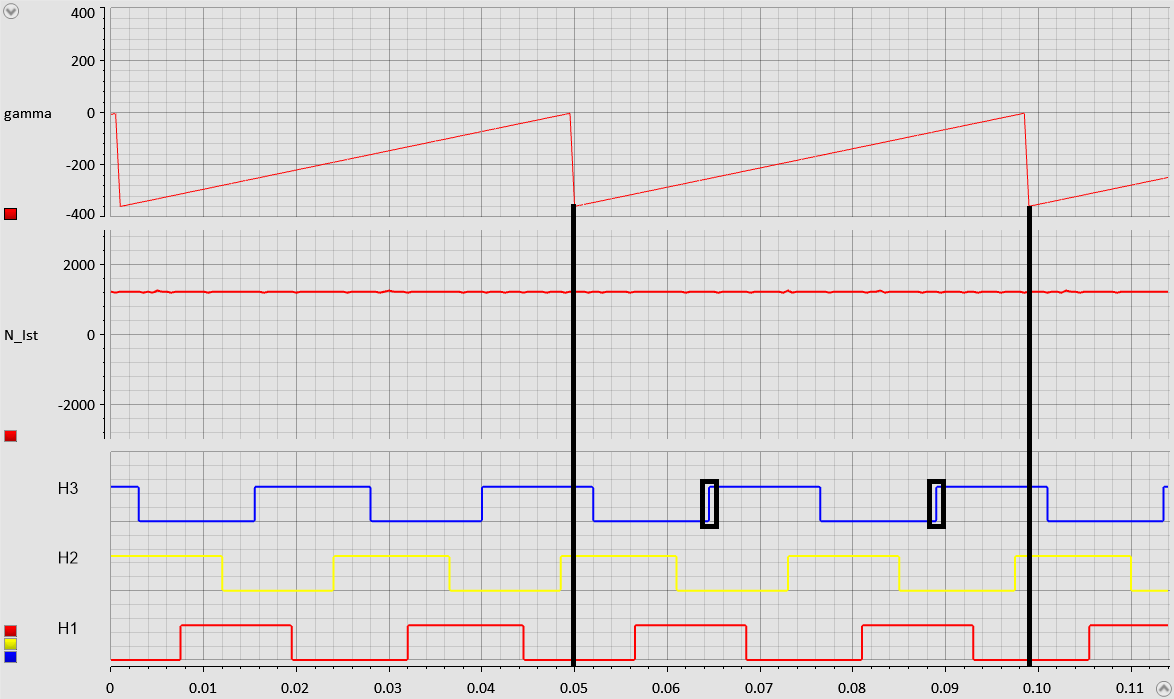
\includegraphics[width=0.99\textwidth]{./Bilder/BLDC_4a_markierung.png}
	\caption{Messung der Hallsensoren am Prüfstand}
	\label{fig:4a:flanken}
\end{figure}

\section{}\label{sec:4b}
\textit{Aufgabe ist es eine Ansteuerung für den Motor zu entwerfen, welche aus den gemessenen Hallsensorsignalen die Ansteuersignale für die Halbbrücken der Leistungselektronik liefert. Stellen Sie unter Verwendung Ihrer Überlegungen aus Aufgabe 2, eben jenen Zusammenhang in einer Tabelle dar.}\\
In Tabelle \ref{tab:4b:werte} sind die Ansteuersignale der Transistoren dargestellt. Wichtig hierbei zu wissen ist, dass sowohl im Zustand „000“, als auch im Zustand „111“, jegliche Transistoren gesperrt sind. Dadurch haben wir sichergestellt, dass dies jeweils sichere Zustände sind. Besonders zu beachten ist auch, dass keine zwei Transistoren eines Strangs gleichzeitig geschaltet werden, da sonst ein Kurzschluss stattfindet.\\
\begin{table}[h]
	\centering
	\begin{tabular}{p{1cm} p{1cm} p{1cm} | p{1cm} p{1cm} p{1cm} p{1cm} p{1cm} p{1cm}}
		&&&&&&&&\\[-1em]
		H1 & H2 & H3 & $ S_{UO} $ & $ S_{UU} $ & $ S_{VO} $ & $ S_{VU} $ & $ S_{WO} $ & $ S_{WU} $ \\
		\hline &&&&&&&&\\[-1em]
		  0 &  0 &  0 &   0 &   0 &   0 &   0 &   0 &   0 \\
		  0 &  0 &  1 &   0 &   0 &   1 &   0 &   0 &   1 \\
		  0 &  1 &  0 &   1 &   0 &   0 &   1 &   0 &   0 \\
		  0 &  1 &  1 &   1 &   0 &   0 &   0 &   0 &   1 \\
		  1 &  0 &  0 &   0 &   1 &   0 &   0 &   1 &   0 \\
		  1 &  0 &  1 &   0 &   1 &   1 &   0 &   0 &   0 \\
		  1 &  1 &  0 &   0 &   0 &   0 &   1 &   1 &   0 \\
		  1 &  1 &  1 &   0 &   0 &   0 &   0 &   0 &   0 \\
	\end{tabular}
	\caption{Wahrheitstabelle zur Ansteuerung der Transistoren}
	\label{tab:4b:werte}
\end{table}

\section{}\label{sec:4c}
Die Ansteuerung des BLDC für den Rechtslauf soll im Folgenden implementiert werden. Dafür haben wir die Schalttabelle erstellt, dem Programm die neuen Werte übergeben und dieses anschließend auf die Steuerung geladen.

\chapter{}
Für die fremderregte Gleichstrommaschine aus unserem Labor soll die Magnetisierungskennlinie $ c_{E}\psi(I_{E}) $ der Erregerspule bestimmt werden.
\section{}
In der Abbildung \ref{fig:5:skript} können wir sehen, dass der Erregerfluss $ \psi $ abhängig vom Erregerstrom $ I_{E} $ ist. Da man hier erkennen kann, dass die beiden Größen nicht proportional zueinander sind, können wir die Magnetisierungskennlie nur wie in der Abbildung \ref{fig:5:skript} dargestellt in einem Diagramm darstellen. Wir wissen auch, dass die Maschinenkonstante $ c_{E} $ eine Konstante ist und deswegen somit unser Magnetisierungskennline genauso wie das Schaubild aussehen soll. Die x-Achse stellt dabei den Erregerstrom $ I_{E} $ dar und die y-Achse $ c_{E}\psi $. Es ist $ I_{E} $ variabel einzustellen und $ c_{E}\psi $ anhand der Gleichung (\ref{eq:4:cepsi}) auszurechnen.

\begin{figure}[h]
	\centering
	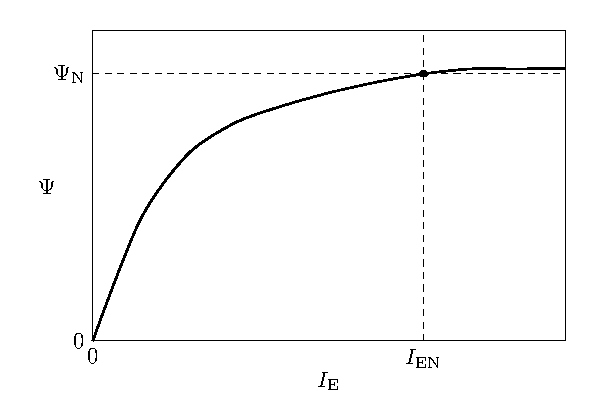
\includegraphics[width=0.65\textwidth]{./bilder/aufgabe5_skript.pdf}
	\caption{Prinzipieller Zusammenhang $ \psi(I_{E}) $ ohne Hysterese, Quelle: \textquotedblleft Elektische Antriebe: Vorlesung zum Sommersemester 2018\textquotedblright, \textit{Prof.–Dr.–Ing. Gernot Schullerus}}
	\label{fig:5:skript}
\end{figure}


\section{}
Wenn man den Erregerstrom $ I_{E} $ herabsetzt, wandert der Betriebspunkt des Motors in den Feldschwächebereich. Die Last kann im Feldschwächebereich jedoch nicht mehr so hoch gewählt werden, trotz dessen dass die Drehzahl des Motors ansteigt. Wird ein kritischer Punkt von $ I_{E} $ unterschritten, so wird die Drehzahl des Motors ins unendliche steigen. Dies führt unweigerlich zur mechanischen Selbstzerstörung des Motors. Aus diesem Grund wurde der Motor im generatorischen Betrieb - mithilfe der Synchronmaschine - betrieben. Somit erhält man eine konstante Drehzahl $ N $.


\section{}
In diesem Aufgabenteil soll die Magnetisierungskennlinie durch eine Exceltabelle mit unseren Messwerten dargestellt werden. Wie in der Aufgabe 4 b) wollen wir hier auch kein Ankerstrom haben. Deshalb haben wir unseren GM mit unserer Lastmaschine betrieben. Dabei haben wir die Drehzahl N konstant auf 1000 Umdrehungen pro Minunte und den Ankerstrom mit einem Intervervall von 0,05A von 0 auf 0,5 A gesetzt. Die Ankerspannung haben wir nach jedem Intervall mit einem Multimeter ausgelesen und diese alle in der Tabelle \ref{tab:5c:cepsi} dargestellt. Anschließend haben wir die Werte in einem Diagramm Abbildung \ref{fig:5c:kennlinie}) dargestellt.  
\begin{table}[h]
	\centering
	\begin{tabular}{p{1.5cm} p{1.5cm} p{1.5cm} p{1.5cm} | p{1.5cm}}
		&&&&\\[-1em]
		$ U_{A}/V $ & $ I_{E} $ & $ N/min^{-1} $ & $ N/s^{-1} $ &  $ c_{E}\Psi/Vs $\\
		\hline &&&&\\[-1em]
		50.5 & 0.47 & 1000 & 16.7 & 3.030\\
		50.1 & 0.45 & 1000 & 16.7 & 3.006\\
		48.8 & 0.40 & 1000 & 16.7 & 2.928\\
		47.4 & 0.35 & 1000 & 16.7 & 2.884\\
		45.5 & 0.30 & 1000 & 16.7 & 2.730\\
		42.9 & 0.25 & 1000 & 16.7 & 2.574\\
		39.1 & 0.20 & 1000 & 16.7 & 2.346\\
		33.0 & 0.15 & 1000 & 16.7 & 1.980\\
		24.2 & 0.10 & 1000 & 16.7 & 1.452\\
		13.2 & 0.05 & 1000 & 16.7 & 0.792\\
		2.0 & 0.00 & 1000 & 16.7 & 0.120		
	\end{tabular}
	\caption{Messwerte für die Magnetisierungskennlinie }
	\label{tab:5c:cepsi}
\end{table}


\begin{figure}[h]
	\centering
	% This file was created by matlab2tikz.
%
%The latest updates can be retrieved from
%  http://www.mathworks.com/matlabcentral/fileexchange/22022-matlab2tikz-matlab2tikz
%where you can also make suggestions and rate matlab2tikz.
%
\definecolor{mycolor1}{rgb}{0.00000,0.44700,0.74100}%
%
\begin{tikzpicture}

\begin{axis}[%
width=3.5in,
height=2.5in,
at={(0.758in,0.481in)},
scale only axis,
xmin=0,
xmax=0.5,
xtick={   0, 0.05,  0.1, 0.15,  0.2, 0.25,  0.3, 0.35,  0.4, 0.45,  0.5},
xlabel style={font=\color{white!15!black}},
xlabel={$ I_{E}/A $},
ymin=0,
ymax=3.5,
ytick={  0, 0.5,   1, 1.5,   2, 2.5,   3, 3.5},
ylabel style={font=\color{white!15!black}},
ylabel={$ c_{E}\Psi/Vs $},
axis background/.style={fill=white},
xmajorgrids,
ymajorgrids,
major grid style={dashed}
]
\addplot [color=mycolor1]
  table[row sep=crcr]{%
0	0.12\\
0.05	0.792\\
0.1	1.452\\
0.15	1.98\\
0.2	2.346\\
0.25	2.574\\
0.3	2.73\\
0.35	2.844\\
0.4	2.928\\
0.45	3.006\\
0.47	3.03\\
};

\end{axis}
\end{tikzpicture}%
	\caption{Kurve der Magnetisierungskennlinie}
	\label{fig:5c:kennlinie}
\end{figure}


\section{}
In den letzten Aufgabenteil soll der Nennpunkt in die Magnetisierungskennlinie eingezeichnet werden und es soll begründet werden, warum der Nennfluss in diesem Bereich festgelegt liegt. Die Arbeitspunkte $ I_{E1} = I_{EN} $ und $ I_{E2} = \frac{1}{2} I_{EN} $ sind auch zu vergleichen.
Der Nennpunkt liegt in unsere Magnetisierungskennlinie am Arbeitspunkt $ I_{E1} = I_{EN} $ (Abbildung \ref{fig:5d:kennlineNenn}). Diese haben wir so bestimmt, indem wir den Erregerstrom so weit erhöht haben, bis sich die Ankerspannung nicht mehr ändert. Dies ist bei $ I_{EN} = 0.47A $ der Fall.
\begin{figure}[h]
	\centering
	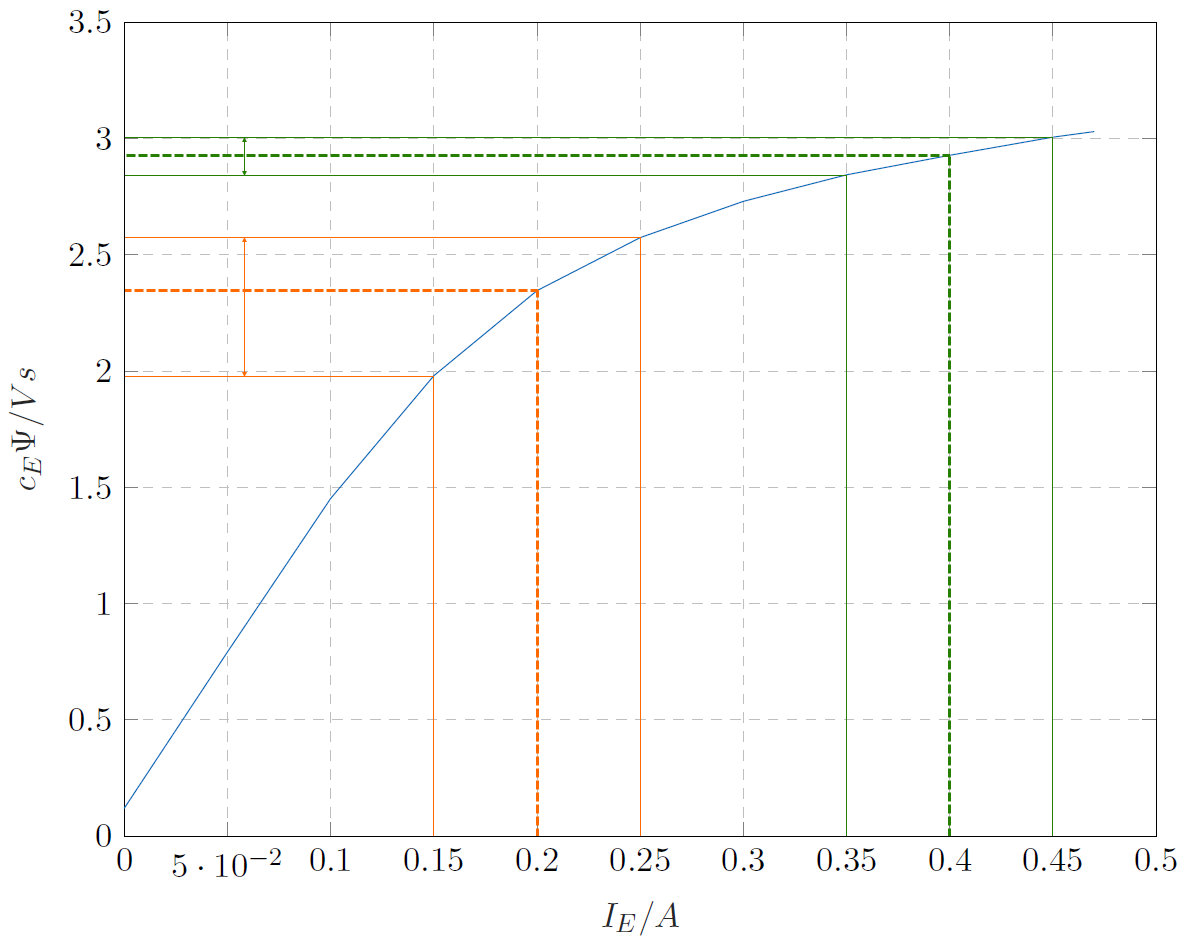
\includegraphics[width=0.7\textwidth]{./bilder/aufgabe4.png}
	\caption{Kurve der Magnetisierungskennlinie mit Nennpunkt}
	\label{fig:5d:kennlineNenn}
\end{figure}

Damit wir den erforderlichen Ankerstrom in den jeweiligen Arbeitspunkte bestimmen können, nehmen wir die Gleichung (\ref{eq:5d:mn}) und formen es nach $ I_{A} $ (\ref{eq:5d:ia}) um. Das Nennmoment $ M_{N} $ haben wir aus den Daten auf dem Leistungsschild berechnet. Näheres dazu wird in der Aufgabenstellung 6 erläutert.
\begin{equation}
	M_{N} = c_{M}\psi I_{A}
	\label{eq:5d:mn}
\end{equation} und stellen nach $ I_{A} $ um, somit ergibt sich die Formel:
\begin{equation}
	I_{A} = \frac{2\pi M_{N}}{c_{E}\psi}
	\label{eq:5d:ia}
\end{equation}
Die Werte in unsere Gleichung eingesetzt ergibt:
\begin{center}
	$ I_{A}(I_{E1}) = \frac{2\pi *1.75Nm}{2.5Vs} = 4.40A $ \\
	$ I_{A}(I_{E2}) = \frac{2\pi *1.75Nm}{3.03Vs} = 3.63A $
\end{center}

In der Abbildung \ref{fig:5d:kennlineNenn} kann man im Arbeitspunkt $ I_{E1} $ erkennen, dass bei Änderungen von $ I_{E} $ von +-50mA, $ \Delta\psi $ deutlich kleiner ist, als im Arbeitspunkt $ I_{E2} $. Somit ist der AP1 günstiger, da es zum einen geringeren Ankerstrom erzeugt und sich somit die Maschine langsamer erwärmt - man muss die GM weniger kühlen. Auch kann man einen kleineren Querschnittsfläche für die Drähte, wegen des kleineren Ankerstroms benutzen. Die geringe Änderung von $ I_{E1} $ heißt auch, dass sie einen geringeren Einfluss auf den Fluss hat und es zu einer stabileren Drehzahl der Gleichstrommaschine führt.
\chapter{}

\section{}
Das Nennmoment lässt sich anhand (\ref{eq:6:MN}) berechnen. Dabei lassen sich die benötigten Parameter vom Typenschild ablesen, wobei die Nenndrehzahl in $ s^{-1} $ umgerechnet werden muss.
\begin{equation}
	M_{N} = \frac{P_{N}}{2\pi N_{N}} = \frac{550W}{2\pi*3000min^{-1}} = \frac{550W}{2\pi*50s^{-1}} \approx 1.75Nm
	\label{eq:6:MN}
\end{equation}
Der Wirkungsgrad im Nennpunkt lässt sich wie in (\ref{eq:6:eta}) durch die zu- und abgeführte Leistung berechnen. Die abgeführte Leistung lässt sich direkt vom Typenschild ablesen, die zugeführte Leistung ergibt sich aus dem Produkt von Ankerspannung und -strom.
\begin{equation}
	\eta_{N} = \frac{P_{ab}}{P_{zu}} = \frac{P_{ab}}{U_{A}I_{A}} = \frac{550W}{180V*4.5A} \approx 67.9\%
	\label{eq:6:eta}
\end{equation}

\begin{figure}[h]
	\centering
	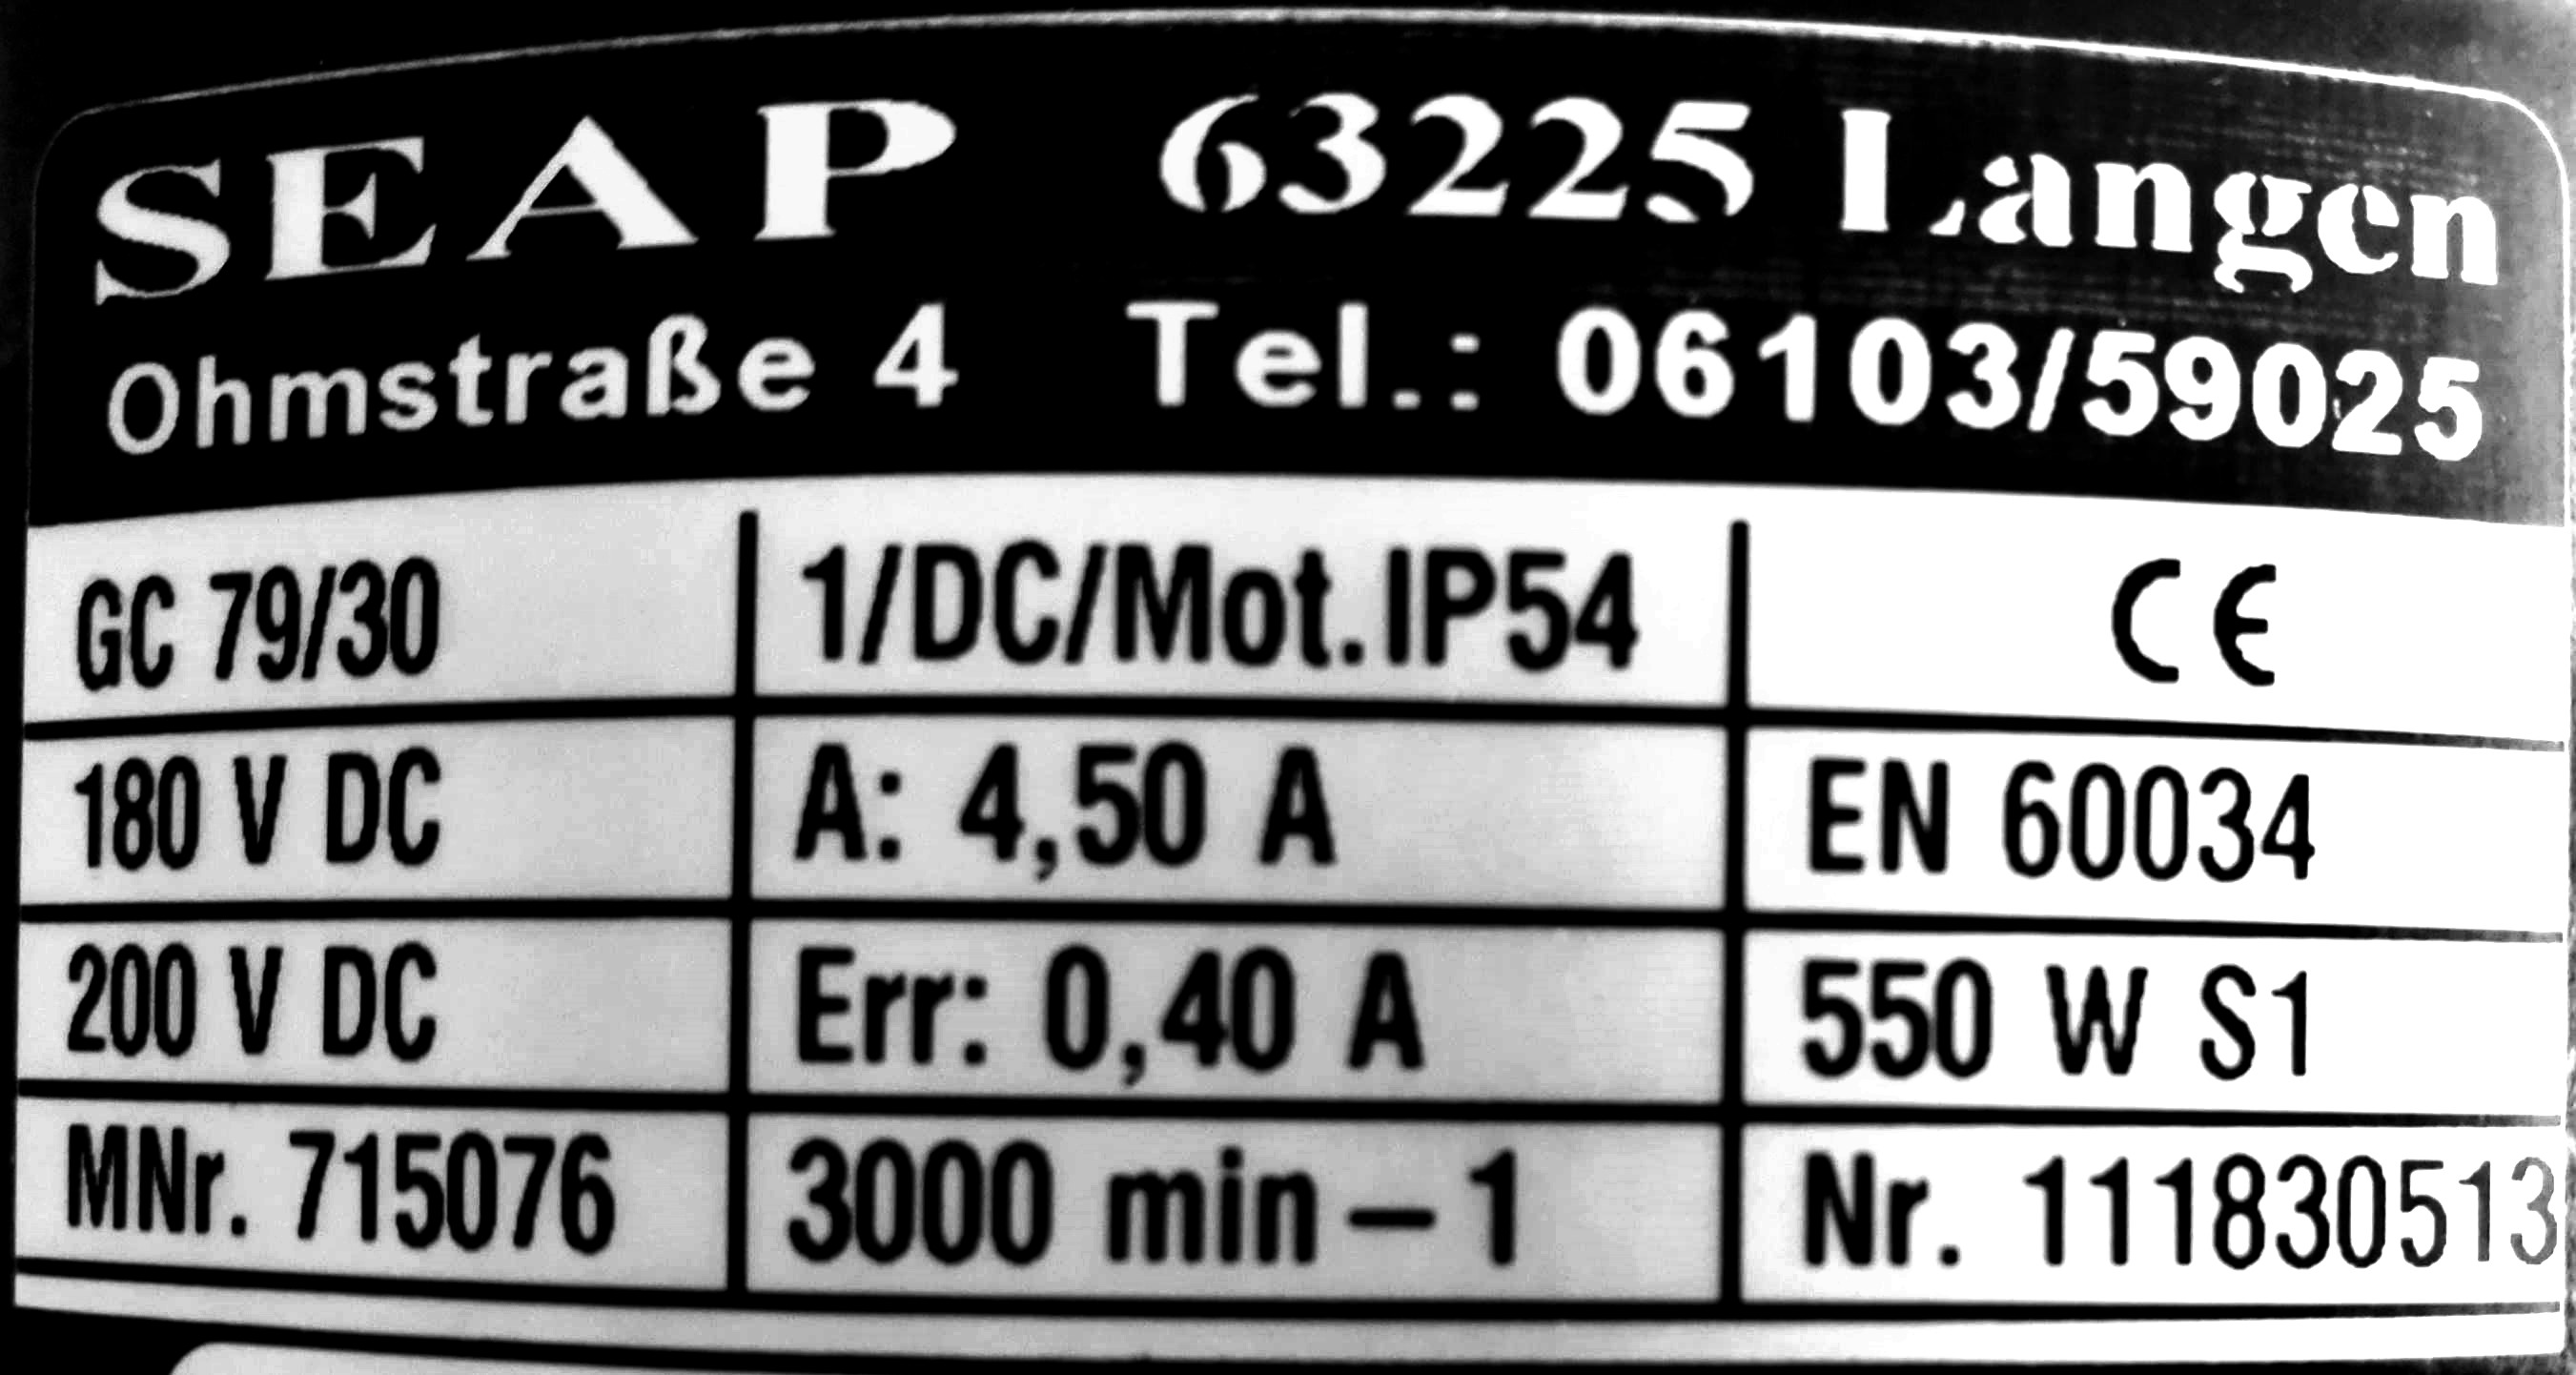
\includegraphics[width=0.5\textwidth]{./bilder/typenschild.jpg}
	\caption{Typenschild}
	\label{fig:typenschild der Gleichstrommaschine}
\end{figure}
\chapter{}
\section{}
In diesem Aufgabenteil soll das Drehzahl-Drehmomentkennlinienfeld der Asynchronmaschine aus dem Versuchsaufbau im Labor Antriebstechnik gemessen werden. Diese wird in der Abbildung 5 dargestellt.
\begin{figure}[h]
	\centering
	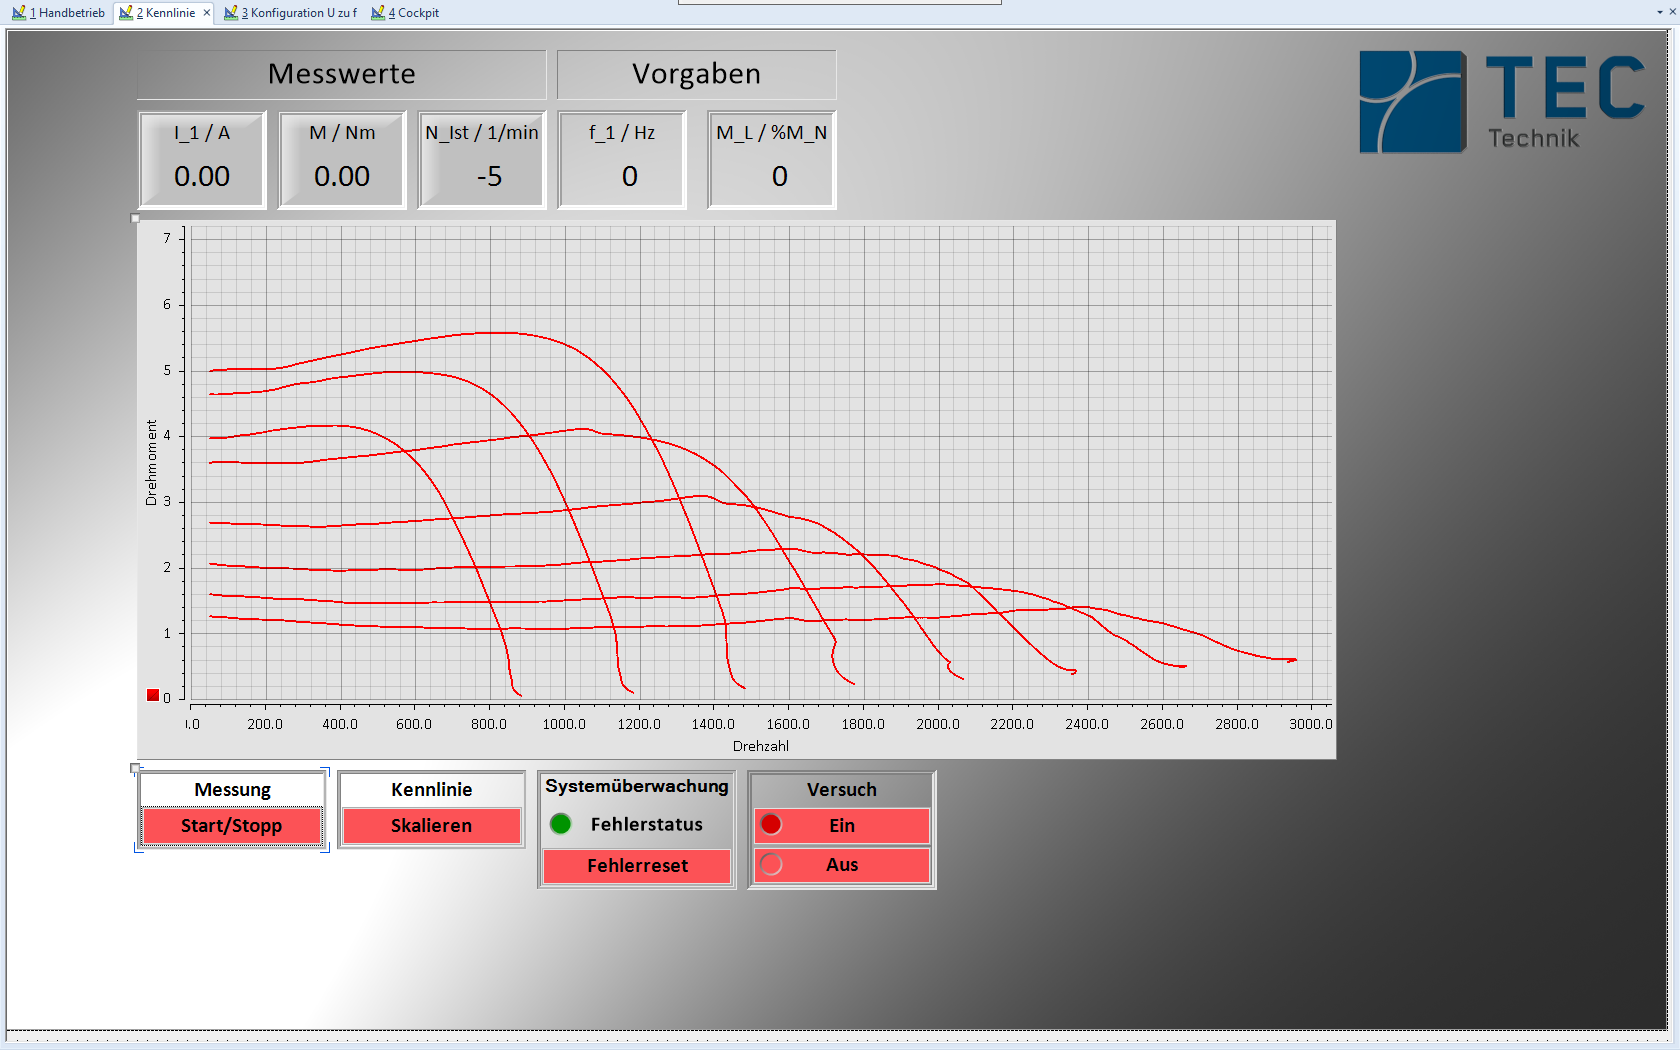
\includegraphics[width=\textwidth]{./Bilder/ele3.png}
	\caption{Drehzahl-Drehmomentkennlinienfeld}
	\label{fig:7a}
\end{figure}

\section{}
Hier wird nun das Kennlinienfeld mit dem Kennlinienfeld aus der Abbildung 6.19 (Skript Elektrische Antriebe) verglichen.\\
Bei geringe Drehzahl $ N $ der Abbildungen zueinander, kann man einen eindeutigen Unterschied erkennen. Dies ist so, weil wir den Idealfall angenommen haben, dass der Statorwiderstand $ R1 = 0\Omega $ sei. Im realen Betrieb ist dies aber nicht der Fall. Der Statorwiderstand hat bei niedrige Statorfrequenzen einen höheren Einfluss auf die Drehmomentkennlinie, da der reale Statorwiderstand für niedrige Statorfrequenzen einen größeren Anteil zur Gesamtimpedanz beiträgt.

\section{}
Im dritten Aufgabenteil soll nun eine Beziehung angegeben werden, wie man bei bekanntem Statorstrombetrag $ I_{1} $ und bekanntem Statorwiderstand $ R_{1} $ der Betrag der Ausgangsspannung $ U_{1} $ verändert werden muss, um dieses Verhalten zu verbessern.

\textbf{???\textit{\underline{???}}}

\section{}
Im letzten Aufgaben Teil haben wir eine erneute Messung mit unseren Anpassung durchgeführt, die wir im dritten Aufgabenteil getroffen haben.\\
In der Abbildung \ref{fig:7d} sieht man nun das Ideale Drehzahl-Drehmomentkennlinienfeld, wo das Drehmoment für kleine Statorfrequenzen kompensiert wurde.
\begin{figure}[h]
	\centering
	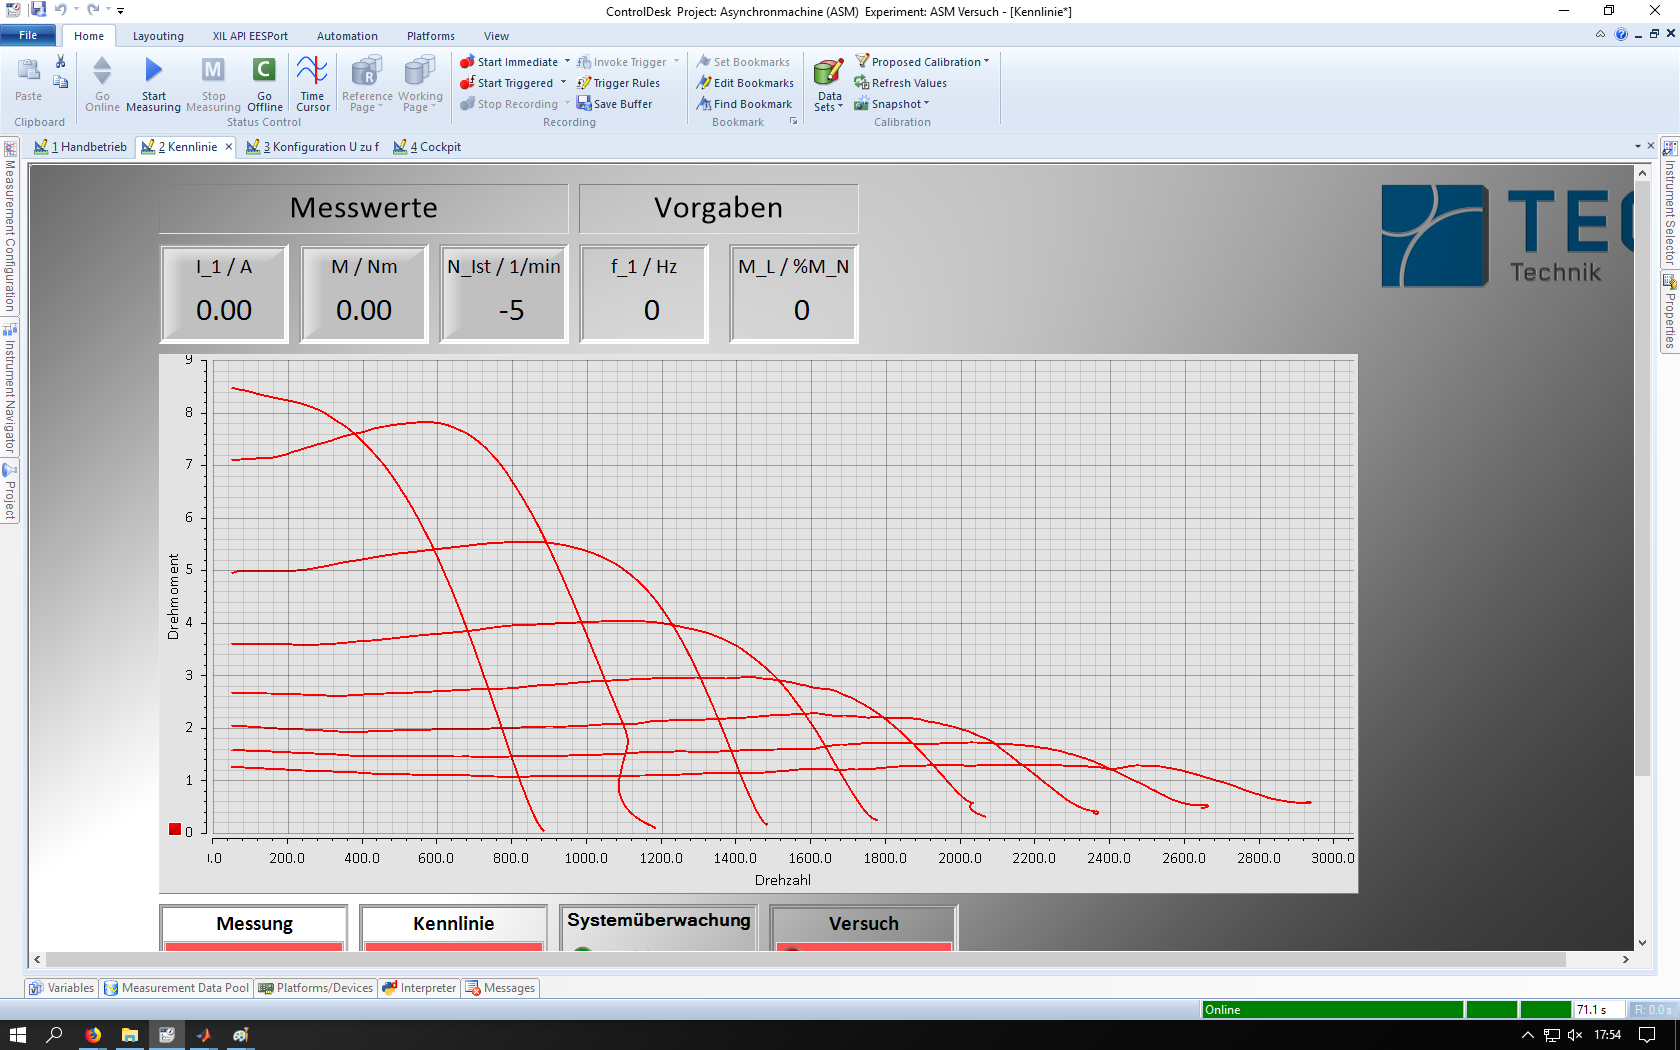
\includegraphics[width=\textwidth]{./Bilder/ele2.png}
	\caption{Drehzahl-Drehmomentkennlinienfeld kompensiert}
	\label{fig:7d}
\end{figure}
%
%und m�glicherweise noch andere Aufgaben
%

%
\end{document}

